\documentclass{monochrome}
\usepackage{lipsum}

\begin{document}

\pagestyle{fancy}
\pagestyle{empty}
\counterwithin{equation}{section}

\newlength\outermarginwidth
\setlength\outermarginwidth{1.5cm}
\newlength\covershift
\setlength\covershift{5cm}

\begin{tikzpicture}[remember picture,overlay]
    \fill[black!90]
    (current page.north west) rectangle (current page.south east);
    \coordinate (start) at ($(current page.east)!0.5!(current page.north east)+(1,-1)$);
    \coordinate (end) at (current page.north west);
    \foreach \i in {0,0.01,...,1}
    {
        \coordinate (point) at ($(start)!\i!(end)$);
        \draw[white]
        ($(point)+(310*\i:6)$)--
        ($(point)+(310*\i+120:6)$)--
        ($(point)+(310*\i+240:6)$)--
        ($(point)+(310*\i:6)$);
    }
    \coordinate (start) at (current page.south west);
    \coordinate (end)   at (current page.east);
    \foreach \i in {0,0.02,...,1}
    {
        \coordinate (point) at ($(start)!\i!(end)$);
        \draw[white]
        ($(point)+(310*\i:10)$)--
        ($(point)+(310*\i+120:10)$)--
        ($(point)+(310*\i+240:10)$)--
        ($(point)+(310*\i:10)$);
    }
    \shade[bottom color=black, top color=black!70, opacity=0.65] ([xshift=.5\outermarginwidth]current page.north west) rectangle (current page.south east);
    \shade[left color=black, right color=black!60, opacity=0.5] ([xshift=\outermarginwidth, yshift=2\outermarginwidth]current page.west) rectangle (current page.south east);
    \fill[white, opacity=0.8]([yshift=2\outermarginwidth]current page.west) rectangle ([xshift=\outermarginwidth, yshift=-.2\outermarginwidth]current page.west);
    \foreach \lx/\rx/\ry/\bc/\tc in {
            1/1.5/1.75/70/80,1.5/2/1.6/65/75,2/2.5/1.3/60/70,2.5/3/1/55/65,3/3.5/.7/50/60,3.5/4/1.2/60/70,4/4.5/1.9/75/85,4.5/5/1.1/55/65,5/5.5/1.2/60/70,6/6.5/1.6/65/75,6.5/7/1.3/60/70,7/7.5/1.87/70/80,7.5/8/1/55/65,8/8.5/.9/50/60,8.5/9/1.8/70/80,9/9.5/1.6/65/75,9.5/10/1.4/60/70,10/10.5/1/55/65,10.5/11/.7/50/60,11/11.5/1.3/55/65,11.5/12/1/70/80,12/12.5/1.3/65/75,12.5/13/1.6/60/70,13/13.5/1.75/55/65,13.5/14/1.6/65/75,14/14.5/1.3/60/70
    }{
        \shade[bottom color=black!\bc,top color=black!\tc,opacity=.5]
        ([xshift=\lx\outermarginwidth]current page.north west) rectangle ([xshift=\rx\outermarginwidth,yshift=-\ry\covershift]current page.north west);
    }
    %%%%%% LETRAS %%%%%
    \node[anchor=south,right] at ([xshift=-5.5\outermarginwidth, yshift=-.457\paperheight]current page.north) {\selectfont           \color{white}\cabin\bfseries\fontsize{95}{95}\selectfont ÁLGEBRA};
    \node[anchor=south,right] at ([xshift=-5.65\outermarginwidth, yshift=-.59\paperheight]current page.north) {\selectfont           \color{white}\cabin\bfseries\fontsize{95}{95}\selectfont LINEAL};
    \node[anchor=west, font=\cabin\fontsize{23}{23}\selectfont, text=white] at ([xshift=1.5\outermarginwidth, yshift=-1.25\covershift]current page.west) {Fundamentos y principios del álgebra lineal};
    \node[anchor=west, font=\cabin\LARGE, text=white] at ([xshift=-1.5\outermarginwidth, yshift=-2.3\covershift]current page.center) {Antonio M. Mendoza ~$\bullet$~ Luis A. Godínez};
    %%%%% LOGO %%%%%
    %\node[anchor=west] at ([xshift=3.25\outermarginwidth, yshift=-2.2\covershift]current page.center) {
\includegraphics[width=3.5cm]{Images/Portada/LOGO.pdf}};
\end{tikzpicture}

\newpage
\,

\newpage

\newgeometry{
	ignorefoot,
	ignorehead,
	left=3cm,
	right=3cm,
	top=3cm,
	bottom=3cm,
	marginparwidth=0cm,
	marginparsep=0mm
}

\begin{tikzpicture}[remember picture,overlay]%
      \coordinate (A) at ($(current page.north)!.4!(current page.north east)$);
      \coordinate (B) at (current page.east);
      \coordinate (C) at (current page.north east);

      \filldraw[black!50] (A) -- (B) -- (C) -- cycle;
      \filldraw ($(current page.north)!.4!(current page.north east)+(0.5,0)$) -- ($(current page.east)+(0,0.25)$) -- (C) -- cycle;
\end{tikzpicture}


\vspace{2cm}
\begin{center}
\scalebox{6.5}{\fontencoding{T1}\fontfamily{pag}\selectfont\textbf{ÁLGEBRA}}\\[10mm]
\scalebox{6.5}{\fontencoding{T1}\fontfamily{pag}\selectfont\textbf{LINEAL}}\\[2cm]

\begin{tabular}{c} \selectfont\cabin\scalebox{2}{Luis Alfonso} \\[2mm] \selectfont\cabin\scalebox{2}{Godínez Contreras} \end{tabular} \hspace{2.5cm} \begin{tabular}{c} \selectfont\cabin\scalebox{2}{Marco Antonio} \\[2mm] \selectfont\cabin\scalebox{2}{Molina Mendoza} \end{tabular}\\[26mm]

\begin{center}
    \begin{tikzpicture}
        \node at (current page.center) {
\includegraphics[width=0.3\textwidth]{Images/Portada/POLITECNICO.pdf}}; % Logo de institución
    \end{tikzpicture}
\end{center}
\fontencoding{T1}\fontfamily{pag}\selectfont Instituto Politécnico Nacional

\vfill
~%México, 2024
\end{center}

\newpage
\,

\newpage

\restoregeometry%

~\vfill\hfill\begin{minipage}[l]{0.72\textwidth}
     \itshape Quiero expresar mi agradecimiento al Lic. Luis Alfonso Godínez Contreras, quien aparte de haber sido mi profesor en algunos cursos, me permitió recopilar el presente trabajo.
\end{minipage}

\newpage
\,

\newpage

\begin{tikzpicture}[remember picture, overlay]%
\fill[black!50] (current page.north west) coordinate (NW) --++(0,-0.15\paperheight) [bend left=-9] to ([shift={(\paperwidth,-.8*0.1\paperheight-2.96cm)}]NW) |- (NW)  --cycle;
\fill[black] (current page.north west) coordinate (NW) --++(0,-0.1\paperheight) [bend left=-10] to ([shift={(\paperwidth,-.8*0.1\paperheight-3.5cm)}]NW) |- (NW)  --cycle;
\pgftext[right,x=11cm,y=-0.75cm]{\altone\fontsize{1.5cm}{1.8cm}\selectfont\color{white}
PREFACIO};%
\end{tikzpicture}
\vspace{3.75cm}

En el ámbito de las ciencias matemáticas, el álgebra lineal emerge como una disciplina fundamental cuya influencia se extiende a diversas áreas del conocimiento. Desde su concepción en los albores del desarrollo matemático hasta su aplicación en campos tan variados como la física teórica, la ingeniería, la economía y la inteligencia artificial, el álgebra lineal ha probado ser un pilar inquebrantable en la comprensión y modelado de fenómenos complejos.

Al abordar la redacción de este texto, he tenido en cuenta la necesidad de equilibrar la claridad expositiva con la profundidad conceptual. Cada capítulo se estructura de manera que los fundamentos se presenten de forma gradual y sistemática, permitiendo al lector asimilar los conceptos básicos antes de adentrarse en temas más complejos. He incorporado numerosos ejemplos, ilustraciones y problemas resueltos para enriquecer la comprensión y facilitar la asimilación de los contenidos.

Este libro también pretende fomentar una apreciación más profunda del álgebra lineal como una disciplina en constante evolución, cuyas aplicaciones van más allá del ámbito académico y se extienden a la resolución de problemas prácticos en la vida cotidiana y en la investigación científica de vanguardia. Se alienta a los lectores a explorar conexiones interdisciplinarias y a aplicar los conceptos aprendidos en contextos diversos, cultivando así una comprensión holística de la materia. El propósito de este libro es servir como recurso educativo y de referencia, cada página de este volumen ha sido meticulosamente diseñada para guiar al lector a través de un viaje intelectual que abarca desde los conceptos más elementales hasta las estructuras más abstractas y sofisticadas.

Esta obra, aunque extensa, está dirigida a estudiantes de Ingeniería, que buscan ampliar su comprensión de esta área de las matemáticas y obtener herramientas prácticas para resolver problemas complejos de la vida real. En este libro se presentan los principios fundamentales de la matemática a través de un enfoque detallado en los apéndices, que abordan temas tan diversos como la inducción matemática, los números complejos, el teorema fundamental del álgebra y la resolución de ecuaciones bajo radicales. Aunque pueden parecer temas adicionales, estos apéndices son esenciales para comprender completamente las teorías matemáticas más avanzadas.

Recalco que esta obra son notas del curso de Álgebra Lineal del periodo 2024/1 y 2024/2, por lo que recomiendo consultar la bibliografía proporcionada en este trabajo. La presente obra consta de todo el contenido que adjudicó el Lic. Luis Alfonso Godinez Contreras, quien imparte clases en la Escuela Superior de Física y Matemáticas (ESFM) en el Instituto Politécnico Nacional (IPN). Hice el mayor esfuerzo en estructurar el libro a base de proposiciones, ejercicios, notas, etc.; y agregué y modifiqué algunas definiciones, a fin de lograr una mayor comprensión sin llegar a tener alguna ambigüedad.

Cabe mencionar que este libro fue mecanografiado por Marco Antonio Molina Mendoza, estudiante de la Escuela Superior de Física y Matemáticas. Sigo trabajando para corregir errores y/o mejorar este trabajo, por lo que está en constante cambio. Recomiendo visitar \href{https://linktr.ee/biblioteca_esfm}{\emph{Biblioteca ESFM}}, un proyecto personal que compila apuntes actualizados. Allí podrán acceder a la última edición del documento.\marginElement{
\begin{center}
    \begin{tikzpicture}
        \node[fill=white] at (0,0) {\hypersetup{hidelinks}\qrcode[hyperlink, height=0.8\linewidth]{https://linktr.ee/biblioteca_esfm}};
    \end{tikzpicture}
\end{center}
}

\newpage
Algunos cambios han sido resultado de los comentarios de mis amigos y estudiantes de la Escuela Superior de Física y Matemáticas. Estas son algunas de las muchas mejoras que he incorporado.
\begin{itemize}
    \item Aspecto estético mejorado: He trabajado arduamente en mejorar el aspecto visual del libro. Incorpore nuevas fuentes y estilos para que sea más fácil de leer y asimilar los conceptos.
    \item Errores ortográficos y matemáticos corregidos: He realizado una revisión minuciosa para garantizar la precisión en todos los aspectos del contenido. Los errores ortográficos y matemáticos se han corregido para ofrecer una experiencia de aprendizaje fluida y confiable.
    \item Imágenes actualizadas: He renovado todas las imágenes y gráficos del libro para asegurarme de que sean claros, informativos y visualmente atractivos. Las nuevas ilustraciones ayudarán a comprender mejor los conceptos y aplicaciones del álgebra lineal en el mundo real.\infoBulle{Las imágenes que se presentan en este libro están hechas con \texttt{TikZ}, una herramienta para la producción de gráficos vectoriales. Dichas imágenes son de elaboración propia y son de dominio público.}
    \item Ejemplos adicionales: He añadido más ejemplos paso a paso y problemas resueltos para reforzar el entendimiento de los temas discutidos.
\end{itemize}

En la elaboración de este libro, he optado por una presentación que refleje la esencia misma de la disciplina: precisión, claridad y elegancia matemática. Con este propósito en mente, he desarrollado una plantilla en LaTeX que resalta la pureza del contenido, utilizando únicamente el contraste entre el blanco y el negro para enfocar la atención en los conceptos fundamentales que exploraremos a lo largo de estas páginas.

La elección de un diseño en blanco y negro no es solo estética, sino una decisión que busca facilitar la comprensión del material para los lectores. Al eliminar cualquier distracción visual que pueda surgir del uso de colores llamativos, me he enfocado en ofrecer una experiencia de lectura que permita una inmersión total en el mundo del álgebra lineal.

Las ecuaciones, teoremas y demostraciones, que constituyen el núcleo de este texto, se presentan de manera clara y legible, sin interferencias visuales. La tipografía se ha seleccionado con cuidado para garantizar una lectura fluida y agradable, mientras que las figuras y gráficos han sido diseñados con precisión para complementar y reforzar los conceptos expuestos en el texto.

Entiendo la importancia de la legibilidad tanto en la versión impresa como en la digital, por lo que he dedicado especial atención a la adaptabilidad de mi plantilla. Ya sea en un libro físico o en un documento electrónico, los lectores encontrarán una presentación coherente y accesible que facilitará su inmersión en los temas tratados.

Con una presentación clara y concisa de los temas, busco fomentar la apreciación de la belleza y utilidad de esta rama de las matemáticas. Se aspira a que los lectores adquieran las habilidades y conocimientos necesarios para resolver problemas complejos y se sientan motivados a explorar aplicaciones más avanzadas del álgebra lineal en su futuro académico y profesional.

Con gratitud y humildad, me complace presentar este volumen a la comunidad académica y a todos aquellos que tienen interés en explorar esta área de las matemáticas. Espero sinceramente que su lectura les resulte tan enriquecedora y reveladora como ha sido para mí su elaboración.

\begin{flushright}
    Marco Antonio Molina Mendoza\\ 
    México, \today\\ 
\end{flushright}

\renewcommand{\contentsname}{CONTENIDO}
\hypersetup{hidelinks}
\TOCPage%
\tableofcontents
\label{toc-contents}
\restoregeometry

\pagestyle{fancy}

\chapter[ESPACIOS VECTORIALES REALES]{ESPACIOS VECTORIALES \\ REALES}\label{chap:ev}

En las páginas siguientes, exploraremos los espacios vectoriales, estructuras fundamentales en matemáticas que sustentan numerosos campos científicos y tecnológicos. Un espacio vectorial real se define mediante diez axiomas básicos, algo que debe comprenderse como un conjunto de principios que no se \emph{demuestran}; más bien, son suposiciones que sirven como punto de partida para desarrollar teoremas.

\section{Definición y ejemplos}

\begin{definicion}{}{espvec}
    Sea $V$ un conjunto no vacío y sea $K$ un campo. Definimos la suma de elementos en $V$ y una multiplicación por un escalar respectivamente, como
    \begin{alignat*}{2}
        + &: & \quad V \times V & \longrightarrow V \\
        & & (\mathbb{u}, \mathbb{v}) & \longmapsto \mathbb{u} + \mathbb{v} \\
        & \\
        \cdot &: & \quad K \times V & \longrightarrow V \\
        & & (\alpha, \mathbb{u}) & \longmapsto \alpha \cdot \mathbb{u}
    \end{alignat*}
    Decimos que $V$ es un \emph{espacio vectorial sobre $K$}, si cumple con los siguientes axiomas: Para toda $\mathbb{x}$, $\mathbb{y}$, $\mathbb{z} \in V$ y $\alpha$, $\beta \in K$
    \begin{enumerate}[label=\roman*), topsep=6pt, itemsep=0pt]
        \item Cerradura: $\mathbb{x} + \mathbb{y} \in V$.
        \item Asociatividad: $\mathbb{x} + (\mathbb{y} + \mathbb {z}) = (\mathbb{x} + \mathbb{y}) + \mathbb{z}$.\newpage
        \item Conmutatividad: $\mathbb{x} + \mathbb{y} = \mathbb{y} + \mathbb{x}$.
        \item Neutro aditivo: Existe un elemento $\mathbb{0} \in V$ que llamaremos cero tal que $\mathbb{x} + \mathbb{0} = \mathbb{0} + \mathbb{x} = \mathbb{x}$.
        \item Inverso aditivo: Para cada $\mathbb{x} \in V$, existe un elemento $-\mathbb{x} \in V$ tal que $\mathbb{x} + (-\mathbb{x}) = \mathbb{0}$. A $-\mathbb{x}$ se le llama inverso de $\mathbb{x}$.
        \item Cerradura: $\alpha \cdot \mathbb{x} \in V$.
        \item Asociatividad: $\alpha \cdot (\beta \cdot \mathbb{x}) = (\alpha \cdot \beta) \cdot \mathbb{x}$.
        \item Distributividad (con un escalar): $\alpha \cdot (\mathbb{x} + \mathbb{y}) = \alpha \mathbb{x} + \alpha \mathbb{y}$.
        \item Distributividad (con dos escalares): $(\alpha + \beta) \cdot \mathbb{x} = \alpha \mathbb{x} + \beta \mathbb{x}$.
        \item Identidad multiplicativa: $1 \cdot \mathbb{x} = \mathbb{x}$.
    \end{enumerate}
\end{definicion}

Si $V$ es un espacio vectorial sobre un campo $K$ y $\mathbb{u} \in V$, entonces diremos que $\mathbb{u}$ es un \emph{vector}. A menos que se indique lo contrario, asumiremos que el campo $K$ es $\RR$, es decir, que trabajamos con espacios vectoriales reales.

\begin{theorem}{}{}
    \TituloBox{Unicidad del neutro y el inverso aditivo:} En un espacio vectorial $V$ sobre $K$, el inverso y el neutro aditivo son únicos.

    \tcblower
    \demostracion Veamos primero que el neutro aditivo es único. Del axioma iv), existe $\mathbb{0} \in V$ tal que para toda $\mathbb{x} \in V$
    \begin{equation}
        \mathbb{x} + \mathbb{0} = \mathbb{0} + \mathbb{x} = \mathbb{x} \label{ec1}
    \end{equation}
    Supongamos que existe $\tilde{\mathbb{0}} \in V$ tal que
    \begin{equation}
        \mathbb{x} + \tilde{\mathbb{0}} = \tilde{\mathbb{0}} + \mathbb{x} = \mathbb{x} \label{ec2}
    \end{equation}
    de \eqref{ec1}, como se cumple para toda $\mathbb{x} \in V$, en particular se cumple para $\mathbb{x} = \tilde{\mathbb{0}}$, es decir
    \begin{equation}
        \tilde{\mathbb{0}} + \mathbb{0} = \mathbb{0} + \tilde{\mathbb{0}} = \tilde{\mathbb{0}} \label{ec3}
    \end{equation}
    de igual forma, de la expresión \eqref{ec2} se cumple para toda $\mathbb{x} \in V$, en particular, para $\mathbb{x} = \mathbb{0}$. Así
    \begin{equation}
        \mathbb{0} + \tilde{\mathbb{0}} = \tilde{\mathbb{0}} + \mathbb{0} = \mathbb{0} \label{ec4}
    \end{equation}
    de \eqref{ec4} y \eqref{ec3},
    \begin{equation*}
        \tilde{\mathbb{0}} \stackrel{\eqref{ec3}}{=} \mathbb{0} + \tilde{\mathbb{0}} \stackrel{\eqref{ec4}}{=} \mathbb{0}
    \end{equation*}
    Por tanto, $\tilde{\mathbb{0}} = \mathbb{0}$. Ahora, demostremos que el inverso es único. Del axioma v), tenemos que para cada $\mathbb{x} \in V$ existe $-\mathbb{x}$ tal que
    \begin{equation}
        \mathbb{x} + (-\mathbb{x}) = \mathbb{0} \label{ec5}
    \end{equation}
    Supongamos que existe $\mathbb{y} \in V$ tal que
    \begin{equation}
        \mathbb{x} + \mathbb{y} = \mathbb{0} \label{ec6}
    \end{equation}
    Demostraremos que $\mathbb{y} = -\mathbb{x}$
    \begin{align*}
        \mathbb{y} & = \mathbb{y} + \mathbb{0} && \text{por axioma iv)} \\
        & = \mathbb{y} + \big( \mathbb{x} + (-\mathbb{x}) \big) && \text{por axioma v)} \\
        & = (\mathbb{y} + \mathbb{x}) + (-\mathbb{x}) && \text{por axioma ii)} \\
        & = (\mathbb{x} + \mathbb{y}) + (-\mathbb{x}) && \text{por axioma iii)} \\
        & = \mathbb{0} + (-\mathbb{x}) && \text{por la expresión \eqref{ec6}} \\
        & = -\mathbb{x} && \text{por axioma iv)}
    \end{align*}
    Por lo tanto, $\mathbb{y} = -\mathbb{x}$.
\end{theorem}

\newpage

\begin{theorem}{}{}
    Sea $V$ un espacio vectorial sobre $K$, entonces
    \begin{enumerate}[label=\roman*., topsep=6pt, itemsep=0pt]
        \item $\alpha \cdot \mathbb{0} = \mathbb{0}$, $\forall \alpha \in K$.
        \item $0 \cdot \mathbb{x} = \mathbb{0}$, $\forall \mathbb{x} \in V$.
        \item Si $\alpha \cdot \mathbb{x} = \mathbb{0}$, entonces $\alpha = 0$ o $\mathbb{x} = \mathbb{0}$.
        \item $(-1) \cdot \mathbb{x} = - \mathbb{x}$.
    \end{enumerate}

    \tcblower
    \demostracion
    \begin{enumerate}[label=\roman*., topsep=6pt, itemsep=0pt]
        \item Sea $\alpha \in K$, tenemos que
        \begin{align}
            \mathbb{0} & = \mathbb{0} + \mathbb{0} && \text{por axioma iv)} \label{ec7} \\
            & = \alpha \cdot \mathbb{0} + (-\alpha \cdot \mathbb{0}) && \text{por axioma v)} \label{ec8}
        \end{align}
        de \eqref{ec7},
        \begin{align}
            \alpha \cdot \mathbb{0} & = \alpha \cdot (\mathbb{0} + \mathbb{0}) && \text{por def. de producto escalar} \label{ec9} \\
            & = \alpha \cdot \mathbb{0} + \alpha \cdot \mathbb{0} && \text{por axioma viii)} \label{ec10}
        \end{align}
        sustituyendo \eqref{ec10} en la ecuación \eqref{ec8}, obtenemos
        \begin{align*}
            \mathbb{0} & = (\alpha \cdot \mathbb{0} + \alpha \cdot \mathbb{0}) + (-\alpha \cdot \mathbb{0}) \\
            & = \alpha \cdot \mathbb{0} + \big( \alpha \cdot \mathbb{0} + (-\alpha \cdot \mathbb{0}) \big) && \text{por axioma ii)} \\
            & = \alpha \cdot \mathbb{0} + \mathbb{0} && \text{por axioma v)} \\
            & = \alpha \cdot \mathbb{0} && \text{por axioma iv)}
        \end{align*}
        Por tanto, $\alpha \cdot \mathbb{0} = \mathbb{0}$.
        \item Sea $\mathbb{x} \in V$. Sabemos que en $K = \RR$, se cumple que $0 + 0 = 0$, ahora
        \begin{align}
            0 \cdot \mathbb{x} & = (0 + 0) \cdot \mathbb{x} && \text{por def. de producto escalar} \label{ec11} \\
            & = 0 \cdot \mathbb{x} + 0 \cdot \mathbb{x} && \text{por ix)} \label{ec12}
        \end{align}
        Por otra parte,
        \begin{align}
            \mathbb{0} & = 0 \cdot \mathbb{x} + (-0 \cdot \mathbb{x}) && \text{por axioma v)} \label{ec13}
        \end{align}
        Sustituyendo \eqref{ec12} en \eqref{ec13},
        \begin{align*}
            \mathbb{0} & = (0 \cdot \mathbb{0} + 0 \cdot \mathbb{0}) + (-0 \cdot \mathbb{x}) \\
            & = 0 \cdot 0 + \big( 0 \cdot \mathbb{x} + (-0 \cdot \mathbb{x}) \big) && \text{por axioma ii)} \\
            & = 0 \cdot \mathbb{x} + 0 && \text{por axioma v)} \\
            & = 0 \cdot \mathbb{x} && \text{por axioma iv)}
        \end{align*}
        Por tanto, $0 \cdot \mathbb{x} = \mathbb{0}$.
        \item Supongamos que $\alpha \neq 0$, entonces hay que demostrar que $\mathbb{x} = \mathbb{0}$. Como $\alpha \in K$ y $\alpha \neq 0$, entonces existe $\alpha^{-1} \in K$ tal que
        \begin{equation}
            \alpha^{-1} \cdot \alpha = 1 \label{ec14}
        \end{equation}
        De la hipótesis,
        \begin{align*}
            \mathbb{0} & = \alpha^{-1} \cdot \mathbb{0} && \text{por (i) de este teorema} \\
            & = \alpha^{-1} \cdot (\alpha \cdot \mathbb{x}) && \text{por hipótesis} \\
            & = (\alpha^{-1} \cdot \alpha) \cdot \mathbb{x} && \text{por axioma vii)} \\
            & = 1 \cdot \mathbb{x} && \text{por ecuación \eqref{ec14}} \\
            & = \mathbb{x} && \text{por axioma x)}
        \end{align*}
        Por tanto, $\mathbb{x} = \mathbb{0}$. Ahora, supongamos que $\mathbb{x} = \mathbb{0}$. Procedamos por reducción al absurdo, supongamos que $\alpha \neq 0$, entonces existe $\alpha^{-1} \in K$ tal que
        \begin{equation}
            \alpha^{-1} \cdot \alpha = 1 \label{ec15}
        \end{equation}
        Entonces
        \begin{align*}
            \mathbb{x} & = 1 \cdot \mathbb{x} && \text{por axioma x)} \\
            & = (\alpha^{-1} \cdot \alpha) \cdot \mathbb{x} && \text{por la ecuación \eqref{ec15}} \\
            & = \alpha^{-1} \cdot (\alpha \cdot \mathbb{x}) && \text{por axioma vii)} \\
            & = \alpha^{-1} \cdot \mathbb{0} && \text{por hipótesis} \\
            & = \mathbb{0}
        \end{align*}
        Por lo tanto, $\mathbb{x} = \mathbb{0}$, como se quería demostrar. Ahora, si $\alpha = 0$ y $\mathbb{x} = \mathbb{0}$, la propiedad (iii) queda demostrada por los incisos (i) y (ii) de este teorema.
        \item Como
        \begin{equation}
            0 = 1 + (-1) \in K \label{ec16}
        \end{equation}
        por (i) de este teorema,
        \begin{align*}
            \mathbb{0} & = 0 \cdot \mathbb{x} \\
            & = \big( 1 + (-1) \big) \cdot \mathbb{x} && \text{por la expresión \eqref{ec16}} \\
            & = 1 \cdot \mathbb{x} +  (-1) \cdot \mathbb{x} && \text{por axioma ix)}
        \end{align*}
        esto es
        \begin{equation}
            \mathbb{0} = 1 \cdot \mathbb{x} + (-1) \cdot \mathbb{x} \label{ec17}
        \end{equation}
        Ahora,
        \begin{align*}
            -\mathbb{x} & = - \mathbb{x} + \mathbb{0} \\
            & = -\mathbb{x} + \big( 1 \cdot \mathbb{x} + (-1) \cdot \mathbb{x} \big) && \text{por la expresión \eqref{ec17}} \\
            & = (-\mathbb{x} + 1 \cdot \mathbb{x}) + (-1) \cdot \mathbb{x} && \text{por axioma ii)} \\
            & = (-\mathbb{x} + \mathbb{x}) + (-1) \cdot \mathbb{x} && \text{por axioma x)} \\
            & = \mathbb{0} + (-1) \cdot \mathbb{x} && \text{por axioma v)} \\
            & = (-1) \cdot \mathbb{x} && \text{por axioma iv)}
        \end{align*}
        Por tanto, $-\mathbb{x} = (-1) \cdot \mathbb{x}$.
    \end{enumerate}
\end{theorem}

En el siguiente ejemplo, demostraremos que $\RR[2]$ es un espacio vectorial sobre $\RR$, verificando que cumple con todas las propiedades que definen un espacio vectorial.\sideFigure[\label{JAJAJJAJS}]{\vspace{6cm}
\begin{center}
    \begin{tikzpicture}%[scale=0.83]
        \coordinate (A) at (1,2.5);
        \coordinate (B) at (2.5,1);
        \coordinate (C) at (3.5,3.5);
        \coordinate (D) at ($1.4*(B)$);
        %
        \draw[thick,-Stealth] (-0.5,0) -- (4.5,0);
        \draw[thick,-Stealth] (0,-0.5) -- (0,4.5);
        \draw[dash pattern=on 3pt off 3pt] (A) -- (C) -- (B);
        \draw[dash pattern=on 3pt off 3pt] (0,3.5) node[left] {$b + d$} -- (3.5,3.5) -- (3.5,0) node[below] {$a + c$};
        \draw[dash pattern=on 3pt off 3pt] (0,2.5) node[left] {$d$} -- (1,2.5) -- (1,0) node[below] {$c$};
        \draw[dash pattern=on 3pt off 3pt] (0,1) node[left] {$b$} -- (2.5,1) -- (2.5,0) node[below] {$a$};
        \draw[-latex] (0,0) -- (A);
        \draw[-latex] (0,0) -- (B);
        \draw[-latex] (0,0) -- (C) node [right] {$\begin{pmatrix} a + c \\ b + d \end{pmatrix}$};
        \draw[-latex] (0,0) -- (D) node [right] {$\begin{pmatrix} \alpha a \\ \alpha b \end{pmatrix}$};
    \end{tikzpicture}
\end{center}
}

\begin{examplebox}{}{}
    Recordemos por el curso de Geometría Analítica que
    $$\RR[2] = \left\{ \begin{pmatrix}
        x \\
        y
    \end{pmatrix} \mid x \in \RR, y \in \RR \right\}$$
    en el cual se definen dos operaciones dados $\mathbb{x}$, $\mathbb{y} \in \RR[2]$ con $\mathbb{x} = \begin{pmatrix}
        a \\
        b
    \end{pmatrix}$ e $\mathbb{y} = \begin{pmatrix}
        c \\
        d
    \end{pmatrix}$
    \begin{alignat*}{2}
        + &: & \quad \RR[2] \times \RR[2] & \longrightarrow \RR[2] \\
        & & (\mathbb{x}, \mathbb{y}) & \longmapsto \begin{pmatrix}
            a + c \\
            b + d
        \end{pmatrix} \\
        & \\
        \cdot &: & \quad \RR \times \RR[2] & \longrightarrow \RR[2] \\
        & & (\alpha, \mathbb{x}) & \longmapsto \begin{pmatrix}
            \alpha a \\
            \alpha b
        \end{pmatrix}
    \end{alignat*}
    Notemos que las operaciones antes mencionadas admiten una interpretación geométrica (vea la figura \ref{JAJAJJAJS}). El conjunto $\RR[2]$ representa el conjunto de todos los pares ordenados de números reales. $\RR[2]$ es bidimensional, lo que significa que tiene dos dimensiones: la dimensión horizontal (eje $x$ por convención) y la dimensión vertical (eje $y$ por convención). En geometría analítica, se utiliza para representar figuras geométricas, ecuaciones de rectas, círculos y cualquier otra forma bidimensional. Probemos que $V = \RR[2]$, con las operaciones “$+$” y “$\cdot$” definidas previamente es un espacio vectorial sobre $\RR$. Verifiquemos los diez axiomas de un espacio vectorial (definición \ref{definicion:espvec}) como sigue:
    \begin{enumerate}[label=\roman*), topsep=6pt, itemsep=0pt]
        \item Sea $\mathbb{x}$, $\mathbb{y} \in \RR[2]$ con $\mathbb{x} = \begin{pmatrix}
            a \\
            b
        \end{pmatrix}$, $\displaystyle \mathbb{y} = \begin{pmatrix}
            c \\
            d
        \end{pmatrix}$, entonces
        \begin{align*}
            \mathbb{x} + \mathbb{y} & = \begin{pmatrix}
                a \\
                b
            \end{pmatrix} + \begin{pmatrix}
                c \\
                d
            \end{pmatrix} \\
            & = \begin{pmatrix}
                a + c \\
                b + d
            \end{pmatrix} && \text{por def. de suma} \\
            & = \begin{pmatrix}
                a + c \\
                b + d
            \end{pmatrix} \in \RR[2]
        \end{align*}
        Ya que $a$, $b$, $c$, $d \in \RR$, entonces $a+c$, $b+d \in \RR$. Por tanto, se cumple la propiedad de cerradura.
        \item Sea $\mathbb{x}$, $\mathbb{y}$, $\mathbb{z} \in \RR[2]$ con $\mathbb{x} = \begin{pmatrix}
            a \\
            b
        \end{pmatrix}$, $\mathbb{y} = \begin{pmatrix}
            c \\
            d
        \end{pmatrix}$, $\mathbb{z} = \begin{pmatrix}
            m \\
            l
        \end{pmatrix}$, entonces
        \begin{align*}
            \mathbb{x} + (\mathbb{y} + \mathbb{z}) & = \begin{pmatrix}
                a \\
                b
            \end{pmatrix} + \left[ \begin{pmatrix}
                c \\
                d
            \end{pmatrix} + \begin{pmatrix}
                m \\
                l
            \end{pmatrix} \right] \\
            & = \begin{pmatrix}
                a \\
                b
            \end{pmatrix} + \begin{pmatrix}
                c + m \\
                d + l
            \end{pmatrix} && \text{por def. de suma} \\
            & = \begin{pmatrix}
                a + (c + m) \\
                b + (d + l)
            \end{pmatrix} && \text{por def. de suma} \\
            & = \begin{pmatrix}
                (a + c) + m \\
                (b + d) + l
            \end{pmatrix} && \text{por asociatividad en $\RR$} \\
            & = \begin{pmatrix}
                a + c \\
                b + d
            \end{pmatrix} + \begin{pmatrix}
                m \\
                l
            \end{pmatrix} && \text{por def. de suma} \\
            & = \left[ \begin{pmatrix}
                a \\
                b
            \end{pmatrix} + \begin{pmatrix}
                c \\
                d
            \end{pmatrix} \right] + \begin{pmatrix}
                m \\
                l
            \end{pmatrix} && \text{por def. de suma} \\
            & = (\mathbb{x} + \mathbb{y}) + \mathbb{z}
        \end{align*}
        Por tanto, se cumple la asociatividad.
        \item Sea $\mathbb{x}$, $\mathbb{y} \in \RR[2]$ con $\mathbb{x} = \begin{pmatrix}
            a \\
            b
        \end{pmatrix}$, $\mathbb{y} = \begin{pmatrix}
            c \\
            d
        \end{pmatrix}$, entonces
        \begin{align*}
            \mathbb{x} + \mathbb{y} & = \begin{pmatrix}
                a \\
                b
            \end{pmatrix} + \begin{pmatrix}
                c \\
                d
            \end{pmatrix} \\
            & = \begin{pmatrix}
                a + c \\
                b + d
            \end{pmatrix} && \text{por def. de suma} \\
            & = \begin{pmatrix}
                c + a \\
                d + b
            \end{pmatrix} && \text{por conmutatividad en $\RR$} \\
            & = \begin{pmatrix}
                c \\
                d
            \end{pmatrix} + \begin{pmatrix}
                a \\
                b
            \end{pmatrix} && \text{por def. de suma} \\
            & = \mathbb{y} + \mathbb{x}
        \end{align*}
        Por tanto, se cumple la conmutatividad.
        \item Sea $\mathbb{0} \in \RR[2]$ con $\mathbb{0} = \begin{pmatrix}
            0 \\
            0
        \end{pmatrix}$, entonces
        \begin{align*}
            \mathbb{0} + \mathbb{x} & = \begin{pmatrix}
                0 \\
                0
            \end{pmatrix} + \begin{pmatrix}
                a \\
                b
            \end{pmatrix} \\
            & = \begin{pmatrix}
                0 + a \\
                0 + b
            \end{pmatrix} && \text{por def. de suma} \\
            & = \begin{pmatrix}
                a \\
                b
            \end{pmatrix} && \text{por neutro aditivo en $\RR$} \\
            & = \mathbb{x}
        \end{align*}
        Por tanto, se cumple la propiedad del neutro aditivo.
        \item Dado $\mathbb{x} = \begin{pmatrix}
            a \\
            b
        \end{pmatrix}$, existe $-\mathbb{x} = \begin{pmatrix}
            -a \\
            -b
        \end{pmatrix} \in \RR[2]$ tal que
        \begin{align*}
            \mathbb{x} + (-\mathbb{x}) & = \begin{pmatrix}
                a \\
                b
            \end{pmatrix} + \begin{pmatrix}
                -a \\
                -b
            \end{pmatrix} \\
            & = \begin{pmatrix}
                a + (-a) \\
                b + (-b)
            \end{pmatrix} && \text{por def. de suma} \\
            & = \begin{pmatrix}
                a - a \\
                b - b
            \end{pmatrix} && \text{por definición en $\RR$} \\
            & = \begin{pmatrix}
                0 \\
                0
            \end{pmatrix} && \text{por inv. aditivo en $\RR$} \\
            & = \mathbb{0}
        \end{align*}
        Por tanto, se cumple la propiedad del inverso aditivo.
        \item Sea $\alpha \in \RR$ y sea $\mathbb{x} \in \RR[2]$ con $\mathbb{x} = \begin{pmatrix}
            a \\
            b
        \end{pmatrix}$, entonces
        \begin{align*}
            \alpha \cdot \mathbb{x} & = \alpha \cdot \begin{pmatrix}
                a \\
                b
            \end{pmatrix} \\
            & = \begin{pmatrix}
                \alpha a \\
                \alpha b
            \end{pmatrix} \in \RR[2] && \text{por def. de producto}
        \end{align*}
        Ya que $\alpha a$, $\alpha b \in \RR$, se cumple la propiedad de cerradura.
        \item Sea $\alpha$, $\beta \in \RR$ y sea $\mathbb{x} \in \RR[2]$ con $\mathbb{x} = \begin{pmatrix}
            a \\
            b
        \end{pmatrix}$, entonces
        \begin{align*}
            \alpha \cdot (\beta \cdot \mathbb{x}) & = \alpha \cdot \left[ \beta \cdot \begin{pmatrix}
                a \\
                b
            \end{pmatrix} \right] \\
            & = \alpha \cdot \left[ \begin{pmatrix}
                \beta a \\
                \beta b
            \end{pmatrix} \right] && \text{por def. de producto} \\
            & = \begin{pmatrix}
                \alpha (\beta a) \\
                \alpha (\beta b)
            \end{pmatrix} && \text{por def. de producto} \\
            & = \begin{pmatrix}
                (\alpha \beta) a \\
                (\alpha \beta) b
            \end{pmatrix} && \text{por asociatividad en $\RR$} \\
            & = (\alpha\beta) \cdot \begin{pmatrix}
                a \\
                b
            \end{pmatrix} && \text{por def. de producto} \\
            & = (\alpha\beta) \cdot \mathbb{x}
        \end{align*}
        Por tanto, se cumple la asociatividad.
        \item Sea $\alpha \in \RR$ y sean $\mathbb{x}$, $\mathbb{y} \in \RR[2]$ con $\mathbb{x} = \begin{pmatrix}
            a \\
            b
        \end{pmatrix}$ e $\mathbb{y} = \begin{pmatrix}
            c \\
            d
        \end{pmatrix}$, entonces
        \begin{align*}
            \alpha \cdot (\mathbb{x} + \mathbb{y}) & = \alpha \cdot \left[ \begin{pmatrix}
                a \\
                b
            \end{pmatrix} + \begin{pmatrix}
                c \\
                d
            \end{pmatrix} \right] \\
            & = \alpha \cdot \begin{pmatrix}
                a + c \\
                b + d
            \end{pmatrix} && \text{por def. de suma} \\
            & = \begin{pmatrix}
                \alpha (a + c) \\
                \alpha (b + d)
            \end{pmatrix} && \text{por def. de producto} \\
            & = \begin{pmatrix}
                \alpha a + \alpha c \\
                \alpha b + \alpha d
            \end{pmatrix} && \text{por distributividad en $\RR$} \\
            & = \begin{pmatrix}
                \alpha a \\
                \alpha c
            \end{pmatrix} + \begin{pmatrix}
                \alpha b \\
                \alpha d
            \end{pmatrix} && \text{por def. de suma} \\
            & = \alpha \cdot \begin{pmatrix}
                a \\
                b
            \end{pmatrix} + \begin{pmatrix}
                c \\
                d
            \end{pmatrix} && \text{por def. de producto} \\
            & = \alpha \cdot \mathbb{x} + \alpha \cdot \mathbb{y}
        \end{align*}
        Por tanto, se cumple la distributividad con dos vectores y un escalar.
        \item Sean $\alpha$, $\beta \in \RR$ y sea $\mathbb{x} \in \RR[2]$ con $\mathbb{x} = \begin{pmatrix}
            a \\
            b
        \end{pmatrix}$, entonces
        \begin{align*}
            (\alpha + \beta) \cdot \mathbb{x} & = (\alpha + \beta) \cdot \begin{pmatrix}
                a \\
                b
            \end{pmatrix} \\
            & = \begin{pmatrix}
                (\alpha + \beta) a \\
                (\alpha + \beta) b
            \end{pmatrix} && \text{por def. de producto} \\
            & = \begin{pmatrix}
                \alpha a + \beta a \\
                \alpha b + \beta b
            \end{pmatrix} && \text{por distributividad en $\RR$} \\
            & = \begin{pmatrix}
                \alpha a \\
                \alpha b
            \end{pmatrix} + \begin{pmatrix}
                \beta a \\
                \beta b
            \end{pmatrix} && \text{por def. de suma} \\
            & = \alpha \cdot \begin{pmatrix}
                a \\
                b
            \end{pmatrix} + \beta \cdot \begin{pmatrix}
                a \\
                b
            \end{pmatrix} && \text{por def. de producto} \\
            & = \alpha \cdot \mathbb{x} + \beta \cdot \mathbb{x}
        \end{align*}
        Por tanto, se cumple la distributividad con dos escalares y un vector.
        \item Sea $\mathbb{x} \in \RR[2]$ con $\mathbb{x} = \begin{pmatrix}
            a \\
            b
        \end{pmatrix}$, entonces
        \begin{align*}
            1 \cdot \mathbb{x} & = 1 \cdot \begin{pmatrix}
                a \\
                b
            \end{pmatrix} \\
            & = \begin{pmatrix}
                1 \cdot a \\
                1 \cdot b
            \end{pmatrix} && \text{por def. de producto} \\
            & = \begin{pmatrix}
                a \\
                b
            \end{pmatrix} && \text{por identidad multiplicactiva en $\RR$} \\
            & = \mathbb{x}
        \end{align*}
        Por tanto, se cumple la propiedad de identidad multiplicativa.
    \end{enumerate}
    Por lo tanto, $\RR[2]$ es un espacio vectorial sobre $\RR$.
\end{examplebox}

La idea de usar pares ordenados y ternas de números reales para representar puntos en el espacio bidimensional y tridimensional era bien conocida en los siglos XVIII y XIX. Al inicio del siglo XX, matemáticos y físicos comenzaron a explorar el uso de espacios “de dimensiones superiores” en matemáticas y física. Hoy en día, incluso el estudiante común está familiarizado con la noción del tiempo como una cuarta dimensión, una idea utilizada por Albert Einstein al desarrollar la teoría general de la relatividad. Actualmente, los físicos que trabajan en el campo de la “teoría de cuerdas” suelen utilizar el espacio de 11 dimensiones en su búsqueda de una teoría unificada que explique cómo funcionan las fuerzas fundamentales de la naturaleza. Gran parte del trabajo restante en esta sección se ocupa de extender la noción del espacio a $n$ dimensiones.

Para explorar estas ideas más a fondo, comenzamos con algo de terminología y notación. El conjunto de todos los números reales puede ser visto geométricamente como una línea. Se le llama la recta real y se denota por $\RR$ o $\RR[1]$. El superíndice refuerza la idea intuitiva de que una línea es unidimensional. El conjunto de todos los pares ordenados de números reales (llamados 2-tuplas) y el conjunto de todas los ternas ordenadas de números reales (llamados 3-tuplas) se denotan como $\RR[2]$ y $\RR[3]$, respectivamente. El superíndice refuerza la idea de que los pares ordenados corresponden a puntos en el plano (bidimensional) y las ternas ordenadas a puntos en el espacio (tridimensional). Geométricamente, un número real $x$ puede ser representado por un punto sobre una línea.
\begin{figure}[h!]
    \centering
    \begin{tikzpicture}
        \draw[black] (0,0) -- (8,0);
        \filldraw[black] (4,0) circle (2pt); 
        \node at (4, -0.5) {$0$};
        \filldraw (6,0) circle (2pt); 
        \node at (6, -0.5) {$x$};
    \end{tikzpicture}
\caption{Representación de un número real $x$}
\end{figure}

Dados $x$, $y \in \RR$, la pareja ordenada $\begin{pmatrix} x \\ y \end{pmatrix}$ puede ser representado por un punto en el plano. Es decir, $\RR[2]$ representa el conjunto de todos los pares ordenados de números reales, lo que esencialmente constituye un plano bidimensional.
\begin{figure}[h!]
    \centering 
    \begin{tikzpicture}
        \draw[thick,-Stealth] (0,0) -- (6,0);
        \draw[thick,-Stealth] (1,-1) -- (1,4);
        
        \filldraw (1,0) circle (2pt) node[below left] {$\begin{pmatrix} 0 \\ 0 \end{pmatrix}$}; 
        \draw[dash pattern=on 3pt off 3pt, thick] (1,2) -- (4,2) -- (4,0);
        \filldraw (4,2) circle(2pt) node[right] {$\begin{pmatrix} x \\ y \end{pmatrix}$};
        \node[left] at (1, 2) {$y$};
        \node[below] at (4, 0) {$x$};
    \end{tikzpicture}
    \caption{Representación de una pareja ordenada $\begin{pmatrix} x \\ y \end{pmatrix}$}
\end{figure}

Dados $x$, $y$, $z \in \RR$, la terna ordenada $\begin{pmatrix} x \\ y \\ z \end{pmatrix}$ puede ser representada por un punto en el espacio. Es decir, $\RR[3]$ es el espacio tridimensional que experimentamos en la vida cotidiana, donde cada punto puede describirse con tres coordenadas reales. 
\begin{figure}[h!]
    \centering 
    \begin{tikzpicture}
        \draw[thick,-Stealth] (0,0) -- (3.5,0);
        \draw[thick,-Stealth] (0,0) -- (0,3.5);
        \draw[thick,-Stealth] (0, 0) -- (-2,-2);
        
        \draw[dash pattern=on 3pt off 3pt] (0,2) -- (2.5,2) -- (2.5,0);
        \draw[dash pattern=on 3pt off 3pt] (-1, 1) -- (1.5, 1) -- (1.5, -1) -- (-1,-1) (-1, 1);
        \draw[dash pattern=on 3pt off 3pt] (-1, 1) -- (-1, -1);
        \draw[thick] (0, 2) -- (-1, 1);
        \draw[thick] (2.5, 2) -- (1.5, 1);
        \draw[thick] (2.5, 0) -- (1.5, -1);
        \node[left] at (0, 2.2) {$z$};
        \node[below] at (2.7, 0) {$y$};
        \node[left] at (-1, -1) {$x$};
        \filldraw (1.5, 1) circle (2pt);
        \draw[ultra thin] (1.6, 1) -- (3.5, 1.2);
        \node[above,fill=white] at (3.5, 0.5) {$\begin{pmatrix} x \\ y \\ z \end{pmatrix}$};
    \end{tikzpicture}
    \caption{Representación de una terna ordenada $\begin{pmatrix} x \\ y \\ z \end{pmatrix}$}
\end{figure}

\newpage

\begin{definicion}{}{}
    Sea $n \in \NN$, definimos
    \begin{matrizn}
        \makecell{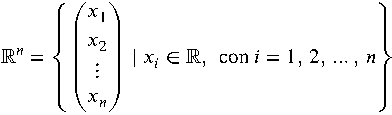
\includegraphics[page=1]{Externalizacion/C1/MatricesC1.pdf}}
    \end{matrizn}
    en donde existen dos operaciones: Dados $\mathbb{x}$, $\mathbb{y} \in \RR[n]$ con \(\mathbb{x} = \begin{pNiceMatrix}[cell-space-limits=3pt] \vphantom{^A}x_1 \\ x_2 \\ \vdots \\ x_n\vphantom{_{A_A}} \end{pNiceMatrix}\) e \(\mathbb{y} = \begin{pNiceMatrix}[cell-space-limits=3pt] \vphantom{^A}y_1 \\ y_2 \\ \vdots \\ y_n\vphantom{_{A_A}} \end{pNiceMatrix}\),
    \begin{matrizn}
        \makecell{\includegraphics[page=2]{Externalizacion/C1/MatricesC1.pdf}}
    \end{matrizn}
    A los números $x_1$, $x_2$, $\dots$, $x_n$ les llamaremos entradas o componentes de $\mathbb{x}$.
\end{definicion}

\begin{definicion}{}{}
    Sean $\mathbb{x}$, $\mathbb{y} \in \RR[n]$. Diremos que $\mathbb{x}$ e $\mathbb{y}$ son \emph{iguales} (también llamado \emph{equivalentes}), denotado por $\mathbb{x} =\mathbb{y}$, si y solo si $x_i = y_i$ para toda $i = 1, 2, \dots, n$. Es decir, si todas las entradas de $\mathbb{x}$ e $\mathbb{y}$ son iguales, entonces $\mathbb{x} = \mathbb{y}$.
\end{definicion}
\sideFigure[\label{HAJAHVSVAVVCAC}Representación geométrica de algunos ejemplos del conjunto $V$]{\vspace{4cm}
\begin{tikzpicture}
    \draw[thick,-Stealth] (-2.5,0) -- (2.5,0) node[below left] {$x$};
    \draw[thick,-Stealth] (0,-2.5) -- (0,2.5) node[below left] {$y$};
    \draw[draw={black!50}] (-2,-2) -- (2,2) node[above] {$y = x$};
    \draw[draw={black!75}] (-1,-2) -- (1,2) node[above] {$y = 2x$};
    \draw[draw={black!50}] (-2,-2/3) -- (2,2/3) node[above] {$y = \dfrac{1}{3}x$};
    \filldraw (0,0) circle (1.75pt) node[below right] {$\begin{pmatrix}
        0 \\
        0
    \end{pmatrix}$};
\end{tikzpicture}
}
\begin{examplebox}{}{}
    Sea
    $$V = \left\{ \begin{pmatrix}
        x \\
        y
    \end{pmatrix} \in \RR[2] \mid y = mx, \text{ con } m \in \RR \text{ fijo} \right\}$$
    con la suma y multiplicación por un escalar definidas en $\RR[2]$. Notemos que la expresión $y = mx$ representa una recta en el plano cartesiano con pendiente $m$ que pasa por el origen, donde $x$ y $y$ son las coordenadas de un punto y $m$ es una constante. Este conjunto admite una interpretación geométrica (vea la figura \ref{HAJAHVSVAVVCAC}). Observemos que
    $$V = \left\{ \begin{pmatrix}
        x \\
        mx
    \end{pmatrix} \in \RR[2] \mid m \in \RR \text{ fijo} \right\}.$$
    Verifiquemos entonces, los diez axiomas de un espacio vectorial. Así:
    \begin{enumerate}[label=\roman*), topsep=6pt, itemsep=0pt]
        \item Sea $\mathbb{x}$, $\mathbb{y} \in V$ con $\mathbb{x} = \begin{pmatrix}
            x \\
            mx
        \end{pmatrix}$, $\mathbb{y} = \begin{pmatrix}
            y \\
            my
        \end{pmatrix}$, entonces
        \begin{align*}
            \mathbb{x} + \mathbb{y} & = \begin{pmatrix}
                x \\
                mx
            \end{pmatrix} + \begin{pmatrix}
                y \\
                my
            \end{pmatrix} \\
            & = \begin{pmatrix}
                x + y \\
                mx + my
            \end{pmatrix} && \text{por def. de suma} \\
            & = \begin{pmatrix}
                x + y \\
                m(x + y)
            \end{pmatrix} && \text{por distributividad en $\RR$} \\
            & = \begin{pmatrix}
                \chi \\
                m\chi
            \end{pmatrix} \in V && \text{siendo $\chi = x + y$}
        \end{align*}
        Por tanto, se cumple la propiedad de cerradura.\newpage
        \item Sea $\mathbb{x}$, $\mathbb{y}$, $\mathbb{z} \in V$ con $\mathbb{x} = \begin{pmatrix}
            m \\
            mx
        \end{pmatrix}$, $\mathbb{y} = \begin{pmatrix}
            y \\
            my
        \end{pmatrix}$, $\mathbb{z} = \begin{pmatrix}
            z \\
            mz
        \end{pmatrix}$, entonces
        \begin{align*}
            \mathbb{x} + (\mathbb{y} + \mathbb{z}) & = \begin{pmatrix}
                x \\
                mx
            \end{pmatrix} + \left[ \begin{pmatrix}
                y \\
                my
            \end{pmatrix} + \begin{pmatrix}
                z \\
                mz
            \end{pmatrix} \right] \\
            & = \begin{pmatrix}
                x \\
                mx
            \end{pmatrix} + \begin{pmatrix}
                y + z \\
                my + mz
            \end{pmatrix} && \text{por def. de suma} \\
            & = \begin{pmatrix}
                x + (y + z) \\
                mx + (my + mz)
            \end{pmatrix} && \text{por def. de suma} \\
            & = \begin{pmatrix}
                (x + y) + z \\
                (mx + my) + mz
            \end{pmatrix} && \text{por asociatividad en $\RR$} \\
            & = \begin{pmatrix}
                x + y \\
                mx + my
            \end{pmatrix} + \begin{pmatrix}
                z \\
                mz
            \end{pmatrix} && \text{por def. de suma} \\
            & = \left[ \begin{pmatrix}
                x \\
                mx
            \end{pmatrix} + \begin{pmatrix}
                y \\
                my
            \end{pmatrix} \right] + \begin{pmatrix}
                z \\
                mz
            \end{pmatrix} && \text{por def. de suma} \\
            & = (\mathbb{x} + \mathbb{y}) + \mathbb{z}
        \end{align*}
        Por tanto, se cumple la asociatividad.
        \item Sea $\mathbb{x}$, $\mathbb{y} \in V$ con $\mathbb{x} = \begin{pmatrix}
            x \\
            mx
        \end{pmatrix}$, $\mathbb{y} = \begin{pmatrix}
            y \\
            my
        \end{pmatrix}$, entonces
        \begin{align*}
            \mathbb{x} + \mathbb{y} & = \begin{pmatrix}
                x \\
                mx
            \end{pmatrix} + \begin{pmatrix}
                y \\
                my
            \end{pmatrix} \\
            & = \begin{pmatrix}
                x + y \\
                mx + my
            \end{pmatrix} && \text{por def. de suma} \\
            & = \begin{pmatrix}
                y + x \\
                my + mx
            \end{pmatrix} && \text{por conmutatividad en $\RR$} \\
            & = \begin{pmatrix}
                y \\
                my
            \end{pmatrix} + \begin{pmatrix}
                x \\
                mx
            \end{pmatrix} && \text{por def. de suma} \\
            & = \mathbb{y} + \mathbb{x}
        \end{align*}
        Por tanto, se cumple la propiedad de conmutatividad.
        \item Existe $\mathbb{0} = \begin{pmatrix}
            0 \\
            m \cdot 0
        \end{pmatrix} \in V$ tal que
        $$\mathbb{x} + \mathbb{0} = \begin{pmatrix}
            x \\
            mx
        \end{pmatrix} + \begin{pmatrix}
            0 \\
            m \cdot 0
        \end{pmatrix} = \mathbb{x}.$$
        El elemento $\mathbb{0}$ pertenece al conjunto $V$ porque cumple con la condición que define a los elementos de $V$, es decir, que la segundo componente sea igual a $m$ multiplicado por el primero. Además, $\mathbb{0}$ actúa como el neutro aditivo porque,
        \begin{align*}
            \mathbb{x} + \mathbb{0} & = \begin{pmatrix}
                x \\
                mx
            \end{pmatrix} + \begin{pmatrix}
                0 \\
                m \cdot 0
            \end{pmatrix} \\
            & = \begin{pmatrix}
                x + 0 \\
                mx + m \cdot 0
            \end{pmatrix} && \text{por def. de suma} \\
            & = \begin{pmatrix}
                x \\
                mx + 0
            \end{pmatrix} && \text{por propiedad en $\RR$} \\
            & = \begin{pmatrix}
                x \\
                mx
            \end{pmatrix} && \text{por neutro aditivo en $\RR$} \\
            & = \mathbb{x}
        \end{align*}
        Por lo tanto, $\mathbb{0}$ existe en $V$ y cumple con la propiedad requerida de ser el elemento neutro para la suma en este espacio.
        \item Para cada $\mathbb{x} = \begin{pmatrix}
            x \\
            mx
        \end{pmatrix} \in V$, existe $-\mathbb{x} = \begin{pmatrix}
            -x \\
            m(-x)
        \end{pmatrix} \in V$ tal que
        $$\mathbb{x} + (-\mathbb{x}) = \begin{pmatrix}
            x \\
            mx
        \end{pmatrix} + \begin{pmatrix}
            -x \\
            m(-x)
        \end{pmatrix} = \mathbb{0}.$$
        Es claro que el elemento $-\mathbb{x}$ pertenece al conjunto $V$ porque cumple con la condición que define a los elementos de $V$, es decir, que el segundo componente sea igual a $m$ multiplicado por el primero. En este caso, para $-\mathbb{x}$, el segundo componente es $m(-x)$. Además, $-\mathbb{x}$ actúa como el opuesto aditivo de $\mathbb{x}$, ya que,
        \begin{align*}
            \mathbb{x} + (-\mathbb{x}) & = \begin{pmatrix}
                x \\
                mx
            \end{pmatrix} + \begin{pmatrix}
                -x \\
                m(-x)
            \end{pmatrix} \\
            & = \begin{pmatrix}
                x + (-x) \\
                mx + m(-x)
            \end{pmatrix} && \text{por def. de suma} \\
            & = \begin{pmatrix}
                x - x \\
                m\big(x + (-x)\big)
            \end{pmatrix} && \text{por distributividad en $\RR$} \\
            & = \begin{pmatrix}
                0 \\
                m \cdot 0
            \end{pmatrix} && \text{por inv. aditivo en $\RR$} \\
            & = \mathbb{0}
        \end{align*}
        Por tanto, se cumple la propiedad del inverso aditivo.
        \item Sea $\alpha \in \RR$ y sea $\mathbb{x} \in V$ con $\mathbb{x} = \begin{pmatrix}
            x \\
            mx
        \end{pmatrix}$, entonces
        \begin{align*}
            \alpha \cdot \mathbb{x} & = \alpha \cdot \begin{pmatrix}
                x \\
                mx
            \end{pmatrix} \\
            & = \begin{pmatrix}
                \alpha x \\
                \alpha mx
            \end{pmatrix} && \text{por def. de producto} \\
            & = \begin{pmatrix}
                (\alpha x) \\
                m(\alpha x)
            \end{pmatrix} && \text{por asociatividad en $\RR$} \\
            & = \begin{pmatrix}
                \xi \\
                m\xi
            \end{pmatrix} \in V && \text{siendo $\xi = \alpha x$}
        \end{align*}
        Por tanto, se cumple la propiedad de cerradura.
        \item Se deja como ejercicio al lector.
        \item Sea $\alpha \in \RR$ y sean $\mathbb{x}$, $\mathbb{y} \in V$ con $\mathbb{x} = \begin{pmatrix}
            x \\
            mx
        \end{pmatrix}$ e $\mathbb{y} = \begin{pmatrix}
            y \\
            my
        \end{pmatrix}$, entonces
        \begin{align*}
            \alpha \cdot (\mathbb{x} + \mathbb{y}) & = \alpha \cdot \left[ \begin{pmatrix}
                x \\
                mx
            \end{pmatrix} + \begin{pmatrix}
                y \\
                my
            \end{pmatrix} \right] \\
            & = \alpha \cdot \begin{pmatrix}
                x + y \\
                mx + my
            \end{pmatrix} && \text{por def. de suma} \\
            & = \begin{pmatrix}
                \alpha (x + y) \\
                \alpha (mx + my)
            \end{pmatrix} && \text{por def. de producto} \\
            & = \begin{pmatrix}
                \alpha x + \alpha y \\
                \alpha mx + \alpha my
            \end{pmatrix} && \text{por distributividad en $\RR$} \\
            & = \begin{pmatrix}
                \alpha x \\
                \alpha mx
            \end{pmatrix} + \begin{pmatrix}
                \alpha y \\
                \alpha my
            \end{pmatrix} && \text{por def. de suma} \\
            & = \alpha \cdot \begin{pmatrix}
                x \\
                mx
            \end{pmatrix} + \alpha \cdot \begin{pmatrix}
                y \\
                my
            \end{pmatrix} && \text{por def. de producto} \\
            & = \alpha \cdot \mathbb{x} + \alpha \cdot \mathbb{y}
        \end{align*}
        Por tanto, se cumple la distributividad con dos vectores y un escalar.
        \item Sea $\alpha$, $\beta \in \RR$ y sea $\mathbb{x} \in V$ con $\mathbb{x} = \begin{pmatrix}
            x \\
            mx
        \end{pmatrix}$, entonces
        \begin{align*}
            (\alpha + \beta) \cdot \mathbb{x} & = (\alpha + \beta) \cdot \begin{pmatrix}
                x \\
                mx
            \end{pmatrix} \\
            & = \begin{pmatrix}
                (\alpha + \beta) \cdot x \\
                (\alpha + \beta) \cdot mx
            \end{pmatrix} && \text{por def. de producto} \\
            & = \begin{pmatrix}
                \alpha x + \beta x \\
                \alpha mx + \beta mx
            \end{pmatrix} && \text{por distributividad en $\RR$} \\
            & = \begin{pmatrix}
                \alpha x \\
                \alpha mx
            \end{pmatrix} + \begin{pmatrix}
                \beta x \\
                \beta mx
            \end{pmatrix} && \text{por def. de suma} \\
            & = \alpha \cdot \mathbb{x} + \beta \cdot \mathbb{x} && \text{por def. de producto}
        \end{align*}
        Por tanto, se cumple la distributividad con dos escalares y un vector.
        \item Sea $\mathbb{x} \in V$ con $\mathbb{x} = \begin{pmatrix}
            x \\
            mx
        \end{pmatrix}$, entonces
        \begin{align*}
            1 \cdot \mathbb{x} & = 1 \cdot \begin{pmatrix}
                x \\
                mx
            \end{pmatrix} \\
            & = \begin{pmatrix}
                1 \cdot x \\
                1 \cdot mx
            \end{pmatrix} && \text{por def. de producto} \\
            & = \begin{pmatrix}
                x \\
                mx
            \end{pmatrix} && \text{por identidad multiplicactiva en $\RR$} \\
            & = \mathbb{x}
        \end{align*}
        Por tanto, se cumple la propiedad de identidad multiplicativa.
    \end{enumerate}
    Por tanto, $V$ es un espacio vectorial sobre $\RR$.
\end{examplebox}
\sideFigure[\label{UAJAJJSHSHHCGTQTTA}Representación geométrica de algunos ejemplos del conjunto $U$]{\vspace{4cm}
\begin{tikzpicture}
    \draw[thick,-Stealth] (-2.5,0) -- (2.5,0) node[below left] {$x$};
    \draw[thick,-Stealth] (0,-2.5) -- (0,2.5) node[below left] {$y$};
    \draw[draw={black!50}] (-2,-1) -- (1,2) node[above right] {$y = x + 1$};
    \draw[draw={black!75}] (-1.5,-2) node[below] {$y = 2x + 1$} -- (0.5,2);
    \draw[draw={black!50}] (-2,1/3) -- (2,5/3) node[below] {$y = \dfrac{1}{3}x + 1$};
    \filldraw (0,1) circle (2pt) node [below right] {$\begin{pmatrix} 0 \\ 1 \end{pmatrix}$};
\end{tikzpicture}
}
\begin{examplebox}{}{}
    Sea
    $$\displaystyle U = \left\{ \begin{pmatrix}
        x \\
        y
    \end{pmatrix} \in \RR[2] \mid y = mx+1, \text{ con }  m \in \RR \text{ fijo} \right\}$$
    con las operaciones de suma y multiplicación por un escalar definidas en $\RR[2]$. Demostremos que $U$ no es un espacio vectorial sobre $\RR$. Obervemos que
    $$U = \left\{ \begin{pmatrix}
        x \\
        mx + 1
    \end{pmatrix} \in \RR[2] \mid m \in \RR \text{ fijo} \right\}$$
    Así, se sigue que:
    \begin{enumerate}[label=\roman*), topsep=6pt, itemsep=0pt]
        \item Sea $\mathbb{x}$, $\mathbb{y} \in V$ con $\mathbb{x} = \begin{pmatrix}
            x \\
            mx + 1
        \end{pmatrix}$, $\mathbb{y} = \begin{pmatrix}
            y \\
            my + 1
        \end{pmatrix}$, entonces
        \begin{align*}
            \mathbb{x} + \mathbb{y} & = \begin{pmatrix}
                x \\
                mx + 1
            \end{pmatrix} + \begin{pmatrix}
                y \\
                my + 1
            \end{pmatrix} \\
            & = \begin{pmatrix}
                x + y \\
                mx + 1 + my + 1
            \end{pmatrix} && \text{por def. de suma} \\
            & = \begin{pmatrix}
                x + y \\
                m(x + y) + 2
            \end{pmatrix} && \text{por distributividad en $\RR$} \\
            & = \begin{pmatrix}
                \chi \\
                m\chi + 2
            \end{pmatrix} \notin U && \text{siendo $\chi = x + y$}
        \end{align*}
        Por tanto, no se cumple la propiedad de cerradura.
    \end{enumerate}
    Por tanto, $U$ no es un espacio vectorial sobre $\RR$. De igual forma al anterior ejemplo, $U$ admite una interpretación geométrica sencilla, vea la figura \ref{UAJAJJSHSHHCGTQTTA}.
\end{examplebox}

El siguiente ejemplo es el espacio vectorial de funciones reales en $(-\infty, \infty)$.

\newpage
\sideFigure[\label{fig:propfunc}]{
    \begin{flushleft}
        \begin{tikzpicture}
            \tikzmath{
                \c = 1.25;
                \a = \c - 1.5;
                \b = \c + 1.5;
                function f(\x) {
                    return -0.1*(\x-\c)^2 + 0.7;
			    };
                function g(\x) {
                    return 0.3*(\x-\c)^2 + 1.7;
			    };
                function h(\x) {
                    return f(\x) + g(\x);
			    };
		    };
            \draw[black,thick] plot[domain = \a:\b, samples = 120] (\x,{f(\x)});
            \draw[black!75,thick] plot[domain = \a:\b, samples = 120] (\x,{g(\x)});
            \draw[black!50,thick] plot[domain = \a:\b, samples = 120] (\x,{h(\x)});
            \draw (\c,0) -- (\c,-0.2) node[below] {$x$};
            %
            \draw[-Stealth,thick] (0,-0.5) -- (0,3.5) node[below right] {$y$};
            \draw[-Stealth,thick] (-1,0) -- (3.5,0) node[below left] {$x$};
            %
            \node[left] at (\a,{f(\a)}) {$\mathbb{f}$};
            \node[left] at (\a,{g(\a)}) {$\mathbb{g}$};
            \node[left] at (\a,{h(\a)}) {$\mathbb{f} + \mathbb{g}$};
            %
            \filldraw[black] (\c,{f(\c)}) circle (2pt);
            \filldraw[black!75] (\c,{g(\c)}) circle (2pt);
            \filldraw[black!50] (\c,{h(\c)}) circle (2pt);
            %
            \draw[black, decorate, decoration={brace,raise=5pt}, transform shape] (\c,0.05) -- node[midway, left, xshift=-7pt] {$f(x)$} (\c,{f(\c)});
            \draw[black, decorate, decoration={brace,mirror,raise=5pt}, transform shape] (\c,0.05) -- node[midway, right, xshift=7pt, yshift=3pt] {$g(x)$} (\c,{g(\c)});
            \draw[black, decorate, decoration={brace,mirror,raise=5pt}, transform shape] (2.1,0.05) -- node[midway, right, xshift=7pt] {$f(x) + g(x)$} (2.1,{h(\c)});
            \node at (0,5) {~};
        \end{tikzpicture}
        \TituloBox{\normalsize(a)}\\[3mm]
        \begin{tikzpicture}
            \tikzmath{
                \c = 1.25;
                \a = \c - 1.5;
                \b = \c + 1.5;
                function f(\x) {
                    return -0.1*(\x-\c)^2 + 0.7;
			    };
                function h(\x) {
                    return 2.5*f(\x);
			    };
		    };
            \draw[black,thick] plot[domain = \a:\b, samples = 120] (\x,{f(\x)});
            \draw[black!75,thick] plot[domain = \a:\b, samples = 120] (\x,{h(\x)});
            \draw (\c,0) -- (\c,-0.2) node[below] {$x$};
            %
            \draw[-Stealth,thick] (0,-0.5) -- (0,3.5) node[below right] {$y$};
            \draw[-Stealth,thick] (-1,0) -- (3.5,0) node[below left] {$x$};
            %
            \node[left] at (\a,{f(\a)}) {$\mathbb{f}$};
            \node[left] at (\a,{h(\a)}) {$\alpha \cdot \mathbb{f}$};
            %
            \filldraw[black] (\c,{f(\c)}) circle (2pt);
            \filldraw[black!50] (\c,{h(\c)}) circle (2pt);
            %
            \draw[black, decorate, decoration={brace,raise=5pt}, transform shape] (\c,0.05) -- node[midway, left, xshift=-7pt] {$f(x)$} (\c,{f(\c)});
            \draw[black, decorate, decoration={brace,mirror,raise=5pt}, transform shape] (\c,0.05) -- node[midway, right, xshift=7pt, yshift=3pt] {$\alpha f(x)$} (\c,{h(\c)});
        \end{tikzpicture}
        \,\\
        \TituloBox{\normalsize(b)}\\[3mm]
        \begin{tikzpicture}
            \tikzmath{
                \c = 1.25;
                \a = \c - 1.5;
                \b = \c + 1.5;
                function f(\x) {
                    return -0.1*(\x-\c)^2 + 0.7;
			    };
                function h(\x) {
                    return -1*f(\x);
			    };
		    };
            \draw[black,thick] plot[domain = \a:\b, samples = 120] (\x,{f(\x)});
            \draw[black!75,thick] plot[domain = \a:\b, samples = 120] (\x,{h(\x)});
            \draw (\c,0) -- (\c,-0.2);
            %
            \draw[black!50,thick] (\a,0) -- (3.4,0);
            \draw[-Stealth,thick] (0,-1.5) -- (0,2.5) node[below right] {$y$};
            \draw[-Stealth,thick] (3.45,0) -- (3.5,0) node[below left] {$x$};
            \draw[white] (-1,0) -- (-0.99,0);
            %
            \node[left] at (\a,{f(\a)}) {$\mathbb{f}$};
            \node[left] at (\a,{h(\a)}) {$-\mathbb{f}$};
            \node[left] at (\a,0) {$\mathbb{0}$};
            %
            \filldraw[black] (\c,{f(\c)}) circle (2pt);
            \filldraw[black!50] (\c,{h(\c)}) circle (2pt);
            %
            \draw[black, decorate, decoration={brace,raise=5pt}, transform shape] (\c,0.05) -- node[midway, left, xshift=-7pt] {$f(x)$} (\c,{f(\c)});
            \draw[black, decorate, decoration={brace,raise=5pt}, transform shape] (\c,{h(\c)}) -- node[midway, left, xshift=-7pt] {$-f(x)$} (\c,-0.05);
        \end{tikzpicture}
        \,\\
        \TituloBox{\normalsize(c)}
    \end{flushleft}
}

\begin{examplebox}{}{ejemplo5.1.8}
    Sea $V$ el conjunto de funciones con valores reales definidas en cada $x$ en el intervalo $(-\infty, \infty)$. Sean $\mathbb{f} = f(x)$ y $\mathbb{g} = g(x)$ dos funciones en $V$ y $\alpha$ un escalar, definimos
    \begin{equation}
        (\mathbb{f} + \mathbb{g})(x) = f(x) + g(x) \label{eq:sumafuncii}
    \end{equation}
    y para $\alpha$,
    \begin{equation}
        (\alpha \cdot \mathbb{f})(x) = \alpha f(x). \label{eq:prodfuncii}
    \end{equation}
    Una forma de interpretar estas operaciones es ver los valores $f(x)$ y $g(x)$ como las “componentes” de $\mathbb{f}$ y $\mathbb{g}$ en el punto $x$. En este caso, las ecuaciones \eqref{eq:sumafuncii} y \eqref{eq:prodfuncii} establecen que dos funciones se suman agregando sus componentes correspondientes, y que una función se multiplica por un escalar multiplicando cada componente por dicho escalar, exactamente como en $\RR[n]$. Esta idea se ilustra en las partes (a) y (b) de la figura \ref{fig:propfunc}. El conjunto $V$ con estas operaciones se denota por el símbolo $F(-\infty, \infty)$. Podemos demostrar que este es un espacio vectorial de la siguiente manera:
    \begin{enumerate}[label=\roman*), topsep=6pt, itemsep=0pt]
        \item El axioma de cerradura para la suma requiere que si sumamos dos funciones definidas en cada $x$ en el intervalo $(-\infty, \infty)$, entonces la suma de esas funciones también deben estar definidas en cada $x$ en el intervalo $(-\infty, \infty)$. Esto se sigue de la fórmula \eqref{eq:sumafuncii}.
        \item Sea $\mathbb{f}$, $\mathbb{g}$, $\mathbb{h} \in V$ con $\mathbb{f} = f(x)$, $\mathbb{g} = g(x)$, $\mathbb{h} = h(x)$,
        \begin{align*}
            [\mathbb{f} + (\mathbb{g} + \mathbb{h})](x) & = f(x) + (g(x) + h(x)) \\
            & = (f(x) + g(x)) + h(x) \\
            & = [(\mathbb{f} + \mathbb{g}) + \mathbb{h}](x)
        \end{align*}
        Por tanto, se cumple la asociatividad sobre la suma de funciones.
        \item Sea $\mathbb{f}$, $\mathbb{g} \in V$ con $\mathbb{f} = f(x)$, $\mathbb{g} = g(x)$,
        \begin{align*}
            (\mathbb{f} + \mathbb{g})(x) & = f(x) + g(x) \\
            & = g(x) + f(x) \\
            & = (\mathbb{g} + \mathbb{f})(x)
        \end{align*}
        Por tanto, se cumple la propiedad de conmutatividad.
        \item Existe una función $\mathbb{0}$ en $F(-\infty, \infty)$, la cual, al sumarse con cualquier otra función $\mathbb{f}$ en $F(-\infty, \infty)$, devuelve $\mathbb{f}$ como resultado. La función cuyo valor en cada punto $x$ del intervalo $(-\infty, \infty)$ es cero cumple con esta propiedad. Geométricamente, el gráfico de la función $\mathbb{0}$ es la línea que coincide con el eje $x$. De esta forma, si tenemos $\mathbb{f}$, $\mathbb{0} \in V$ con $\mathbb{f} = f(x)$, $\mathbb{0} = 0$,
        \begin{align*}
            (\mathbb{f} + \mathbb{0})(x) & = f(x) + 0 \\
            & = f(x) \\
            & = \mathbb{f}
        \end{align*}
        Por tanto, se cumple la propiedad de neutro aditivo.
        \item Para cada función $\mathbb{f}$ en $F(-\infty, \infty)$ existe una función $-\mathbb{f}$ en $F(-\infty, \infty)$, la cual, al sumarse con $\mathbb{f}$, produce la función $\mathbb{0}$. La función definida por $-\mathbb{f}(x) = -f(x)$ cumple con esta propiedad. Geométricamente, el gráfico de $-\mathbb{f}$ se obtiene reflejando el de $\mathbb{f}$ con respecto al eje $x$ (figura \ref{fig:propfunc}c). Así,
        \begin{align*}
            [\mathbb{f} + (-\mathbb{f})](x) & = f(x) + (-f(x)) \\
            & = f(x) - f(x) \\
            & = 0 \\
            & = \mathbb{0}
        \end{align*}
        Por tanto, se cumple la propiedad de inverso aditivo.
        \item Es análogo al inciso (i) y esto se sigue de la fórmula \eqref{eq:prodfuncii}.
        \item Sea $\mathbb{f}$, $\mathbb{g} \in V$ con $\mathbb{f} = f(x)$, $\mathbb{g} = g(x)$ y sea $\alpha \in \RR$,
        \begin{align*}
            [\alpha \cdot (\mathbb{f} + \mathbb{g})](x) & = \alpha (f(x) + g(x)) \\
            & = \alpha f(x) + \alpha g(x) \\
            & = (\alpha \cdot \mathbb{f})(x) + (\alpha \cdot \mathbb{g})(x) \\
            & = (\alpha \cdot \mathbb{f} + \alpha \cdot \mathbb{g})(x)
        \end{align*}
        Por tanto, se cumple la distributividad sobre la suma de vectores.
        \item Sea $\mathbb{f} \in V$ con $\mathbb{f} = f(x)$ y sea $\alpha$, $\beta \in \RR$,
        \begin{align*}
            [(\alpha + \beta) \cdot \mathbb{f}](x) & = (\alpha + \beta) f(x) \\
            & = \alpha f(x) + \beta f(x) \\
            & = (\alpha \cdot \mathbb{f})(x) + (\beta \cdot \mathbb{f})(x) \\
            & = (\alpha \cdot \mathbb{f} + \beta \cdot \mathbb{f})(x)
        \end{align*}
        Por tanto, se cumple la distributividad sobre la suma de escalares.
        \item Se deja como ejercicio al lector.
        \item Sea $\mathbb{f} \in V$ con $\mathbb{f} = f(x)$ y sea $1 \in \RR$,
        \begin{align*}
            (1 \cdot \mathbb{f})(x) & = 1 f(x) \\
            & = f(x) \\
            & = \mathbb{f}
        \end{align*}
        Por tanto, se cumple la propiedad de identidad multiplicativa.
    \end{enumerate}
    Dado que $F(-\infty, \infty)$ satisface todas las propiedades requeridas para ser un espacio vectorial, concluimos que $F(-\infty, \infty)$ es un espacio vectorial sobre $\RR$.
\end{examplebox}

Es crucial entender que no se pueden imponer arbitrariamente dos operaciones en un conjunto $V$ y esperar que se cumplan los axiomas de espacio vectorial. Por ejemplo, si $V$ es el conjunto de vectores de $\RR[n]$ con componentes positivas y se usan las operaciones estándar de $\RR[n]$, entonces $V$ no es cerrado bajo la multiplicación por escalares, ya que $(-1) \cdot \mathbb{u}$ es un vector con al menos un componente negativo, que no pertenecería a $V$.

El siguiente es un ejemplo menos evidente en el que solo uno de los diez axiomas de espacio vectorial deja de cumplirse.

\begin{examplebox}{}{}
    Sea $V = \RR[2]$ y definamos las operaciones de suma y producto escalar en $V$ de la siguiente manera: Si $\mathbb{u} = \begin{pmatrix}
        u_1 \\
        u_2
    \end{pmatrix}$, $\mathbb{v} = \begin{pmatrix}
        v_1 \\
        v_2
    \end{pmatrix}$ y si $\alpha$ es un número real cualquiera,
    $$\mathbb{u} + \mathbb{v} = \begin{pmatrix}
        u_1 + v_1 \\
        u_2 + v_2
    \end{pmatrix} \quad \text{ y } \quad \alpha \cdot \mathbb{u} = \begin{pmatrix}
        \alpha u_1 \\
        0
    \end{pmatrix}.$$
    Por ejemplo, si $\mathbb{u} = \begin{pmatrix}
        2 \\
        4
    \end{pmatrix}$, $\mathbb{v} = \begin{pmatrix*}[r]
        -3 \\
        5
    \end{pmatrix*}$ y $\alpha = 7$, entonces
    $$\mathbb{u} + \mathbb{v} = \begin{pmatrix}
        2 + (-3) \\
        4 + 5
    \end{pmatrix} = \begin{pmatrix*}[r]
        -1 \\
        9
    \end{pmatrix*} \quad \text{ y } \quad \alpha \cdot \mathbb{u} = 7 \cdot \mathbb{u} = \begin{pmatrix}
        7 \cdot 2 \\
        0
    \end{pmatrix} = \begin{pmatrix}
        14 \\ 
        0
    \end{pmatrix}.$$
    La operación de suma es la estándar en $\RR[2]$, pero el producto escalar no lo es. Los primeros nueve axiomas se cumplen, sin embargo, el axioma (x) no se cumple para ciertos vectores. Por ejemplo, si $\mathbb{u}$ es tal que $u_2 \neq 0$, entonces
    $$1 \cdot \mathbb{u} = 1 \cdot \begin{pmatrix}
        u_1 \\
        u_2
    \end{pmatrix} = \begin{pmatrix}
        1 \cdot u_1 \\
        0
    \end{pmatrix} = \begin{pmatrix}
        u_1 \\
        0
    \end{pmatrix} \neq \mathbb{u}.$$
    Por lo tanto, $V$ no es un espacio vectorial con las operaciones establecidas.
\end{examplebox}

\newpage

Nuestro siguiente ejemplo será un espacio vectorial inusual que hemos incluido para ilustrar la variedad de espacios vectoriales.

\begin{examplebox}{}{}
    Sea $V$ el conjunto de los números reales positivos, y sean $\mathbb{u} = u$ y $\mathbb{v} = v$ cualesquiera vectores (es decir, números reales positivos) en $V$. Sea $\alpha$ un escalar cualquiera. Definimos las operaciones en $V$ como
    $$\mathbb{u} + \mathbb{v} = uv \quad \text{ y } \quad \alpha \cdot \mathbb{u} = u^{\alpha}.$$
    Por ejemplo, $1 + 1 = (1)(1) = 1$ y $(2)(1) = 1^2 = 1$, lo cual resulta extraño, pero, no obstante, el conjunto $V$ con estas operaciones satisface los diez axiomas de los espacios vectoriales y, por lo tanto, es un espacio vectorial. Verificaremos algunos axiomas, y dejaremos los demás como ejercicio al lector.
    \begin{enumerate}[label=\roman*), topsep=6pt, itemsep=0pt]
        \item Dado que $\mathbb{u} = u$ y $\mathbb{v} = v$ son números reales positivos, el producto $uv$ es también un número real positivo, ya que el producto de dos números reales positivos siempre da como resultado otro número real positivo.
        \item Sea $\mathbb{u}$, $\mathbb{v} \in V$ con $\mathbb{u} = u$, $\mathbb{v} = v$,
        \begin{align*}
            \mathbb{u} + \mathbb{v} & = uv \\
            & = vu \\
            & = \mathbb{v} + \mathbb{u}
        \end{align*}
        Por tanto, se cumple la propiedad de conmutatividad.
        \item Se deja como ejercicio al lector.
        \item Sea $\mathbb{u}$, $\mathbb{0} \in V$ con $\mathbb{u} = u$, $\mathbb{0} = 1$,
        \begin{align*}
            \mathbb{u} + \mathbb{0} & = u^1 \\
            & = u \\
            & = \mathbb{u}
        \end{align*}
        Por tanto, se cumple la propiedad de neutro aditivo.
        \item Dado $\mathbb{u} = u$, existe $-\mathbb{u} = \dfrac{1}{u}$ que satisface
        \begin{align*}
            \mathbb{u} + (-\mathbb{u}) & = u \left( \frac{1}{u} \right) \\
            & = 1 \\
            & = \mathbb{0}
        \end{align*}
        Por tanto, se cumple la propiedad de inverso aditivo.
        \item Dado que $\mathbb{u} = u$ es un número real positivo, y $\alpha$ es un número real cualquiera, la operación $u^{\alpha}$ es también un número real positivo.
        \item Sea $\mathbb{u}$, $\mathbb{v} \in V$ con $\mathbb{u} = u$, $\mathbb{v} = v$ y sea $\alpha \in \RR$,
        \begin{align*}
            \alpha \cdot (\mathbb{u} + \mathbb{v}) & = (uv)^{\alpha} \\
            & = u^{\alpha} v^{\alpha} \\
            & = \alpha \cdot \mathbb{u} + \alpha \cdot \mathbb{v}
        \end{align*}
        Por tanto, se cumple la distributividad sobre la suma de vectores.
        \item Sea $\mathbb{u} \in V$ con $\mathbb{u} = u$ y sea $\alpha$, $\beta \in \RR$,
        \begin{align*}
            (\alpha + \beta) \cdot \mathbb{u} & = u^{\alpha + \beta} \\
            & = u^{\alpha} u^{\beta} \\
            & = \alpha \cdot \mathbb{u} + \beta \cdot \mathbb{u}
        \end{align*}
        Por tanto, se cumple la distributividad sobre la suma de escalares.
        \item Se deja como ejercicio al lector.
        \item Se deja como ejercicio al lector.
    \end{enumerate}
    En conclusión, aunque estas operaciones resulten inusuales, la verificación de los diez axiomas, confirma que esta estructura cumple con todos los requisitos para ser considerada un espacio vectorial sobre $\RR$.
\end{examplebox}

El siguiente ejemplo es el espacio vectorial de los polinomios con coeficientes reales, que cumple con los axiomas correspondientes.

\begin{examplebox}{}{POLIREALES}
    El conjunto de polinomios reales de grado menor o igual a $n$ se define como
    $$P_n = \left\{ a_nx^n + a_{n-1}x^{n-1} + \cdots + a_1x + a_0 \mid a_i \in \RR, \text{ para } i = 0, 1, 2, \dots, n \right\}$$
    y se expresan los elementos como
    $$p(x) = a_nx^n + a_{n-1}x^{n-1} + \cdots + a_1x + a_0$$
    En $P_n$, definimos dos operaciones: Dado $p(x) \in P_n$ y $\alpha \in \RR$,
    \begin{alignat*}{2}
        + & : & \quad P_n \times P_n & \longrightarrow P_n \\
        & & \big(p(x), q(x) \big) & \longmapsto p(x)+q(x) \\
        & \\
        \cdot & : & \quad \RR \times P_n & \longrightarrow P_n \\
        & & \big(\alpha, p(x) \big) & \longmapsto \alpha \cdot p(x)
    \end{alignat*}
    donde
    $$p(x) + q(x) = (a_n + b_n)x^n + (a_{n-1} + b_{n-1})x^{n-1} + \cdots + (a_1 + b_1)x + (a_0 + b_0)$$
    y
    $$\alpha \cdot p(x) = \alpha a_nx^n + \alpha a_{n-1}x^{n-1} + \cdots + \alpha a_1x + \alpha a_0.$$
    Entonces $P_n$ es un espacio vectorial sobre $\RR$. Es obvio que la suma de dos polinomios de grado menor o igual a $n$ es otro polinomio de grado menor o igual a $n$, por lo que se cumple el axioma (i). Las propiedades (ii) y (v) a (x) son claras. Si se define el polinomio
    $$\mathbb{0} = 0 x^n+0 x^{n-1} + \cdots + 0 x + 0,$$
    entonces $\mathbb{0} \in P_n$ y el axioma (iii) se cumple. Por último, sea
    $$-p(x) = -a_n x^n - a_{n-1} x^{n-1} - \cdots - a_1 x - a_0;$$
    se ve que el axioma (iv) se cumple, con lo que $P_n$ es un espacio vectorial real.
\end{examplebox}

Nuestro último ejemplo es el más sencillo, ya que corresponde al espacio vectorial cero. A diferencia de los ejemplos anteriores, más complejos, este caso se verifica de manera trivial, ya que solo contiene el vector nulo.

\begin{examplebox}{}{}
    Sea $W$ un conjunto que consta de un único elemento, $\mathbb{0}$, y definimos
    $$\mathbb{0} + \mathbb{0} = \mathbb{0} \quad \text{ y } \quad \alpha \cdot \mathbb{0} = \mathbb{0}$$
    para todo escalar $\alpha$. A esto lo llamamos el \emph{espacio vectorial cero}.
\end{examplebox}

\section{Subespacios vectoriales}

A menudo ocurre que algún espacio vectorial de interés está contenido dentro de un espacio vectorial más grande cuyas propiedades son conocidas. En esta sección mostraremos cómo reconocer cuándo ocurre esto, explicaremos cómo las propiedades del espacio vectorial más grande pueden usarse para obtener propiedades del espacio vectorial más pequeño, y proporcionaremos una variedad de ejemplos.

\newpage

\begin{definicion}{}{}
    Se dice que $W$ es un \emph{subespacio vectorial} de $V$ si $W$ es un subconjunto no vacío de $V$, y $W$ es un espacio vectorial, junto con las operaciones de suma entre vectores y multiplicación por un escalar definidas para $V$.
\end{definicion}

En general, para demostrar que un conjunto no vacío $W$ con dos operaciones es un espacio vectorial, se deben verificar los diez axiomas de espacio vectorial. Sin embargo, si $W$ es un subespacio de un espacio vectorial conocido $V$, entonces ciertos axiomas no necesitan ser verificados porque son “heredados” de $V$. Por ejemplo, no es necesario verificar que $\mathbb{u} + \mathbb{v} = \mathbb{v} + \mathbb{u}$ se cumple en $W$ porque se cumple para todos los vectores en $V$, incluidos los de $W$. Por otro lado, es necesario verificar que $W$ está cerrado bajo la suma y la multiplicación escalar, ya que es posible que sumar dos vectores en $W$ o multiplicar un vector en $W$ por un escalar produzca un vector en $V$ que no esté en $W$ (figura \ref{JAJJAJAJAJJQJQOOQPQZ}).
\begin{figure}[h!]
    \centering
    \begin{tikzpicture}
        \coordinate (A) at (0,2);
        \coordinate (B) at (5,0);
        \coordinate (C) at (7,1.5);
        \coordinate (D) at (2,3.5);
        %
        \draw (A) -- (B) node[above] {$V$} -- (C) -- (D) -- cycle;
        \filldraw[black!7!white] ($(C)!.78!(A)$) -- ($(D)!.78!(B)$) -- ($(A)!.78!(C)$) -- ($(B)!.78!(D)$) -- cycle;
        \draw ($(C)!.78!(A)$) -- ($(D)!.78!(B)$) node[above] {$W$} -- ($(A)!.78!(C)$) -- ($(B)!.78!(D)$) -- cycle;
        \filldraw (3.25,1.5) circle (1.5pt);
        \draw[-latex] (3.25,1.5) -- node[midway,below] {$\mathbb{v}$} (4,1.75);
        \draw[-latex] (3.25,1.5) -- node[midway,left] {$\mathbb{u}$} (2.8,2.4);
        \draw[-latex] (3.25,1.5) -- (3.55,2.65);
        \draw[dashed] (2.8,2.4) -- (3.55,2.65) -- (4,1.75);
        \draw[-latex] (2.8,2.4) -- node[midway,left] {$\alpha \mathbb{u}$} (2.4,3.2);
        \draw[thin] (3.5,2) -- (4.5,2.75) node[above] {$\mathbb{u} + \mathbb{v}$};
    \end{tikzpicture}
    \caption{Los vectores $\mathbb{u}$ y $\mathbb{v}$ están en $W$, pero los vectores $\mathbb{u} + \mathbb{v}$ y $\alpha \mathbb{u}$ no lo están}
    \label{JAJJAJAJAJJQJQOOQPQZ}
\end{figure}

\noindent Los axiomas que no son heredados por $W$ son:
\begin{itemize}
    \item \textbf{Axioma 1:} Cerradura de $W$ bajo la suma.
    \item \textbf{Axioma 4:} Existencia de un vector cero en $W$.
    \item \textbf{Axioma 5:} Existencia de un negativo en $W$ para cada vector en $W$.
    \item \textbf{Axioma 6:} Cerradura de $W$ bajo la multiplicación escalar.
\end{itemize}
Por lo tanto, estos deben ser verificados para probar que $W$ es un subespacio de $V$. Sin embargo, el siguiente teorema muestra que si los axiomas 1 y 6 se cumplen en $W$, entonces los axiomas 4 y 5 se cumplen en $W$ como consecuencia.

\begin{theorem}{}{JAJSUJGBUHBOSOIOOSK}
    Si $W$ es un conjunto de uno o más vectores en un espacio vectorial $V$, entonces $W$ es un subespacio de $V$ si y solo si se satisfacen las siguientes condiciones:
    \begin{enumerate}[label=\alph*), topsep=6pt, itemsep=0pt]
        \item Si $\mathbb{u}$ y $\mathbb{v}$ son vectores en $W$, entonces $\mathbb{u} + \mathbb{v}$ está en $W$.
        \item Si $\alpha$ es un escalar y $\mathbb{u}$ es un vector en $W$, entonces $\alpha \cdot \mathbb{u}$ está en $W$.
    \end{enumerate}

    \tcblower
    \demostracion Por definición, un subespacio es un espacio vectorial cuyos elementos pertenecen a $V$ y cuyas operaciones son las mismas que en $V$. Como $V$ es un espacio vectorial, se tiene que $W$ está cerrado bajo la suma y el producto escalar, que corresponden exactamente a las condiciones (a) y (b). Recíprocamente, supongamos que se satisfacen las condiciones (a) y (b). Dado que los axiomas (i), (ii), (iii), (vii), (viii), (ix) y (x) son heredados de $V$, solo necesitamos demostrar que los axiomas (iv) y (v) se cumplen en $W$. Para ello, sea $\mathbb{u}$ un vector cualquiera en $W$. De la condición (b) se sigue que $\alpha \cdot \mathbb{u}$ es un vector en $W$ para cualquier escalar $\alpha$. En particular, $0 \cdot \mathbb{u} = \mathbb{0}$ y $(-1) \cdot \mathbb{u} = -\mathbb{u}$ están en $W$, lo que muestra que los axiomas (iv) y (v) se cumplen en $W$. 
\end{theorem}

\begin{examplebox}{}{}
    Si $V$ es un espacio vectorial y $W = \{ \mathbb{0} \}$ es el subconjunto de $V$ que consiste únicamente en el vector cero, entonces $W$ está cerrado bajo la suma y la multiplicación por un escalar, ya que
    $$\mathbb{0} + \mathbb{0} = \mathbb{0} \quad \text{ y } \quad \alpha \cdot \mathbb{0} = \mathbb{0}$$
    para cualquier escalar $\alpha$. A $W$ lo llamamos el \emph{subespacio cero} de $V$.
\end{examplebox}

\newpage

\begin{examplebox}{}{}
    Si $W$ es una recta que pasa por el origen en $\RR[2]$ o $\RR[3]$, entonces la suma de dos vectores en la recta o la multiplicación de un vector en la recta por un escalar produce otro vector en la recta. Por lo tanto, $W$ está cerrado bajo la suma y el producto escalar (véase la figura \ref{fig:rectaEV} para una ilustración en $\RR[3]$).
    \begin{center}
        \begin{tikzpicture}
            \draw[thick] (-0.5,-0.25) -- (3.75,1.875) node[right] {$W$};
            \draw[-latex,draw={black!50},thick] (0,0) -- (1,0.5) node[above left] {$\mathbb{u}$};
            \draw[-latex,draw={black!50},thick] (1,0.5) -- (2,1) node[above left] {$\mathbb{v}$};
            \draw[-latex,draw={black!50},thick] (2,1) -- (3,1.5) node[above left] {$\mathbb{u} + \mathbb{v}$};
            \draw[-Stealth,thick] (0,0) -- (0,3) node[below right] {$y$};
            \draw[-Stealth,thick] (0,0) -- (4.2,0) node[below left] {$x$};
            \draw[-Stealth,thick] (0,0) -- (-0.65,-0.9) node[above left] {$z$};
        \end{tikzpicture}
        \hfill
        \begin{tikzpicture}
            \draw[thick] (-0.5,-0.25) -- (3.75,1.875) node[right] {$W$};
            \draw[-latex,draw={black!50},thick] (0,0) -- (1,0.5) node[above left] {$\mathbb{u}$};
            \draw[-latex,draw={black!50},thick] (1,0.5) -- (2.5,1.25) node[above left] {$\alpha \cdot \mathbb{u}$};
            \draw[-Stealth,thick] (0,0) -- (0,3) node[below right] {$y$};
            \draw[-Stealth,thick] (0,0) -- (4.2,0) node[below left] {$x$};
            \draw[-Stealth,thick] (0,0) -- (-0.65,-0.9) node[above left] {$z$};
        \end{tikzpicture}
        
        \TituloBox{(a)} $W$ es cerrado bajo la suma \hfill \TituloBox{(b)} $W$ es cerrado bajo el producto escalar\captionsetup*[figure]{hypcap=false}
        \captionof{figure}{Los vectores $\mathbb{u} + \mathbb{v}$ y $\alpha \cdot \mathbb{u}$ están en la misma recta que $\mathbb{u}$ y $\mathbb{v}$}\label{fig:rectaEV}
    \end{center}
\end{examplebox}

\begin{examplebox}{}{}
    Si $\mathbb{u}$ y $\mathbb{v}$ son vectores en un plano $W$ que pasa por el origen en $\RR[3]$, entonces es evidente geométricamente que $\mathbb{u} + \mathbb{v}$ y $\alpha \cdot \mathbb{u}$ también pertenecen al mismo plano $W$ para cualquier escalar $\alpha$ (figura \ref{fig:planoEV}). Por lo tanto, $W$ está cerrado bajo la suma y el producto escalar.
    \begin{center}
        \begin{tikzpicture}
            \filldraw[black!7!white] (4.25,3) -- (0.75,3) -- (-0.25,-1) -- (3.25,-1) -- cycle;
            \draw[dashed] (1,2) -- (3,2.5) -- (2,0.5);
            \draw[-latex,draw={black!50},thick] (0,0) -- (2,0.5) node[below] {$\mathbb{u}$};
            \draw[-latex,draw={black!50},thick] (0,0) -- (3,0.75) node[below] {~~$\alpha \cdot \mathbb{u}$};
            \draw[-latex,draw={black!50},thick] (0,0) -- (1,2) node[above left] {$\mathbb{v}$};
            \draw[-latex,draw={black!50},thick] (0,0) -- (3,2.5) node[above left] {$\mathbb{u} + \mathbb{v}$};
            \draw[-Stealth,thick] (0,0) -- (0,3.5) node[below right] {$y$};
            \draw[-Stealth,thick] (0,0) -- (4.2,0) node[below left] {$x$};
            \draw[-Stealth,thick] (0,0) -- (-0.65,-0.9) node[above left] {$z$};
            \node[above left] at (3.25,-1) {$W$};
        \end{tikzpicture}
        \captionsetup*[figure]{hypcap=false}
        \captionof{figure}{Los vectores $\mathbb{u} + \mathbb{v}$ y $\alpha \cdot \mathbb{u}$ están en el mismo plano que $\mathbb{u}$ y $\mathbb{v}$}\label{fig:planoEV}
    \end{center}
\end{examplebox}

La tabla \ref{tab:subespR23} a continuación presenta una lista de los subespacios de $\RR[2]$ y $\RR[3]$ que hemos encontrado hasta ahora.
\begin{table}[H]
    \centering
    \begin{NiceTabular}{ll}[cell-space-limits=2pt]
        \CodeBefore
        \rowcolor{black!20!white}{1}
        \Body
        \toprule
        Subespacios de $\RR[2]$ & Subespacios de $\RR[3]$ \\
        \midrule
        $\bullet$\quad $\{ \mathbb{0} \}$ & $\bullet$\quad $\{ \mathbb{0} \}$ \\
        $\bullet$\quad Rectas que pasan por el origen & $\bullet$\quad Rectas que pasan por el origen \\
        $\bullet$\quad $\RR[2]$ & $\bullet$\quad Planos que pasan por el origen \\
        & $\bullet$\quad $\RR[3]$ \\
        \bottomrule
    \end{NiceTabular}
    \caption{Subespacios vectoriales de $\RR[2]$ y $\RR[3]$}
    \label{tab:subespR23}
\end{table}

En los ejemplos anteriores, hemos visto subespacios vectoriales en los espacios $\RR[2]$ y $\RR[3]$. Estos subespacios son fundamentales para comprender las propiedades estructurales de los espacios vectoriales. A continuación, daremos un ejemplo que ilustra cómo el conjunto de funciones continuas, bajo ciertas operaciones, también forma un subespacio.

\begin{examplebox}{}{EJEMPLOINI}
    Existe un teorema en cálculo que establece que la suma de funciones continuas es continua y que una constante multiplicada por una función continua también es continua. En lenguaje vectorial, el conjunto de funciones continuas en $(-\infty, \infty)$ es un subespacio de $F(-\infty, \infty)$. Denotaremos este subespacio como $C(-\infty, \infty)$.
\end{examplebox}

\newpage

\begin{examplebox}{}{}
    Una función con una derivada continua se dice que es \emph{continuamente diferenciable}. Existe un teorema en cálculo que establece que la suma de dos funciones continuamente diferenciables es continuamente diferenciable y que una constante multiplicada por una función continuamente diferenciable también es continuamente diferenciable. Por lo tanto, las funciones que son continuamente diferenciables en $(-\infty, \infty)$ forman un subespacio de $F(-\infty, \infty)$. Denotaremos este subespacio por $C^1(-\infty, \infty)$, donde el superíndice enfatiza que las primeras derivadas son continuas. Para llevar esto un paso más allá, el conjunto de funciones con $m$ derivadas continuas en $(-\infty, \infty)$ es un subespacio de $F(-\infty, \infty)$, al igual que el conjunto de funciones con derivadas de todos los órdenes en $(-\infty, \infty)$. Denotaremos estos subespacios por $C^m(-\infty, \infty)$ y $C^\infty(-\infty, \infty)$, respectivamente.
\end{examplebox}

\begin{examplebox}{}{}
    Recordemos que un \emph{polinomio} es una función que puede expresarse en la forma
    $$p(x) = a_0 + a_1x + \cdots + a_nx^n$$
    donde $a_0, a_1, \dots, a_n$ son constantes. Es evidente que la suma de dos polinomios es un polinomio y que una constante multiplicada por un polinomio también es un polinomio. Por lo tanto, el conjunto $W$ de todos los polinomios es un subespacio de $F(-\infty, \infty)$. Este espacio se denota por $P_\infty$.
\end{examplebox}

\begin{examplebox}{}{EJEMPLOFIN}
    Recordemos que el grado de un polinomio es la mayor potencia de la variable que aparece con un coeficiente distinto de cero. No es cierto que el conjunto $W$ de polinomios de grado exacto $n$ sea un subespacio de $F(-\infty, \infty)$ porque ese conjunto no está cerrado bajo la suma. Por ejemplo, los polinomios
    $$1 + 2x + 3x^2 \quad \text{ y } \quad 5 + 7x - 3x^2$$
    tienen grado $2$, pero su suma tiene grado $1$. Sin embargo, para cada entero no negativo $n$, el conjunto de polinomios de grado menor o igual a $n$ forma un subespacio de $F(-\infty, \infty)$, ya que está cerrado bajo la suma y multiplicación por un escalar.
\end{examplebox}

En nuestros ejemplos anteriores consideramos funciones que estaban definidas en todos los puntos del intervalo $(-\infty, \infty)$. A veces querremos considerar funciones que están definidas únicamente en algún subintervalo de $(-\infty, \infty)$, como el intervalo cerrado $[a, b]$ o el intervalo abierto $(a, b)$. En tales casos, realizaremos un cambio de notación apropiado. Por ejemplo, $C[a, b]$ es el espacio de funciones continuas en $[a, b]$, y $C(a, b)$ es el espacio de funciones continuas en $(a, b)$.

En cálculo se demuestra que los polinomios son funciones continuas y tienen derivadas continuas de todos los órdenes en $(-\infty, \infty)$. Por lo tanto, se deduce que $P_\infty$ no solo es un subespacio de $F(-\infty, \infty)$, como se observó anteriormente, sino que también es un subespacio de $C^\infty(-\infty, \infty)$. Dejamos al lector la tarea de convencerse de que los espacios vectoriales discutidos en los ejemplos \ref{examplebox:EJEMPLOINI} a \ref{examplebox:EJEMPLOFIN} están “anidados” unos dentro de otros, como se ilustra en la figura \ref{JAJAIQPAPOAOSOOAKJS}.
\begin{figure}[h!]
    \centering
    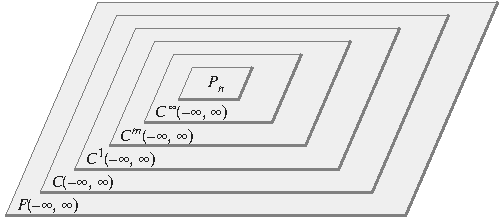
\includegraphics[width=\textwidth]{Images/Capitulo1/AnidadosBN.pdf}
    \caption{Jerarquía de espacios funcionales por diferenciabilidad}
    \label{JAJAIQPAPOAOSOOAKJS}
\end{figure}

\newpage

\begin{theorem}{}{intersubsV}
    Si $W_1, W_2, \dots, W_r$ son subespacios de un espacio vectorial $V$, entonces la intersección de estos subespacios también es un subespacio de $V$.

    \tcblower
    \demostracion Sea $W = W_1 \cap W_2 \cap \cdots \cap W_r$. Este conjunto no es vacío porque cada uno de estos subespacios contiene el vector cero de $V$, y por lo tanto, también lo hace su intersección. Así, queda por demostrar que $W$ está cerrado bajo la suma y la multiplicación por escalares. Para demostrar la cerradura bajo la suma, sean $\mathbb{u}$ y $\mathbb{v}$ vectores en $W$. Dado que $W$ es la intersección de $W_1, W_2, \dots, W_r$, se deduce que $\mathbb{u}$ y $\mathbb{v}$ también pertenecen a cada uno de estos subespacios. Además, como estos subespacios están cerrados bajo la suma y la multiplicación por escalares, también contienen los vectores $\mathbb{u} + \mathbb{v}$ y $\alpha \cdot \mathbb{u}$ para todo escalar $\alpha$, y por lo tanto, su intersección $W$ también los contiene. Esto prueba que $W$ está cerrado bajo la suma y la multiplicación por escalares.
\end{theorem}

\section{Conjuntos generadores}

\begin{definicion}{}{}
    Sea $V$ un espacio vectorial sobre $K$. Si $\mathbb{u}$ es un vector en un espacio vectorial $V$, entonces se dice que $\mathbb{u}$ es una \emph{combinación lineal} de los vectores $\mathbb{v}_1, \mathbb{v}_2, \dots, \mathbb{v}_n$ en $V$ si $\mathbb{u}$ puede expresarse en la forma
    $$\mathbb{u} = k_1 \mathbb{v}_1 + k_2 \mathbb{v}_2 + \cdots + k_n \mathbb{v}_n,$$
    donde $k_1, k_2, \dots, k_n$ son escalares. Estos escalares se denominan los \emph{coeficientes} de la combinación lineal.
\end{definicion}

Si $n = 1$, entonces la expresión de la anterior definición tiene la forma
$$\mathbb{w} = k_1\mathbb{v}_1,$$
en cuyo caso la combinación lineal es simplemente un múltiplo escalar de $\mathbb{v}_1$.

\begin{theorem}{}{CONMAPEQ}
    Sea $V$ un espacio vectorial sobre $K$. Si $S = \{\mathbb{v}_1, \mathbb{v}_2, \dots, \mathbb{v}_n\}$ es un conjunto no vacío de vectores en $V$, entonces:
    \begin{enumerate}[label=\alph*), topsep=6pt, itemsep=0pt]
        \item El conjunto $W$ de todas las combinaciones lineales posibles de los vectores en $S$ es un subespacio de $V$.
        \item El conjunto $W$ en el inciso anterior, es el subespacio más pequeño de $V$ que contiene a todos los vectores en $S$, en el sentido de que cualquier otro subespacio que contenga esos vectores también contiene a $W$.
    \end{enumerate}

    \tcblower
    \demostracion
    \begin{enumerate}[label=\alph*), topsep=6pt, itemsep=0pt]
        \item Sea $W$ el conjunto de todas las combinaciones lineales posibles de los vectores en $S$. Debemos demostrar que $W$ está cerrado bajo la suma y la multiplicación por escalares. Para demostrar la cerradura bajo la suma, sean
        $$\mathbb{x}_1 = a_1\mathbb{v}_1 + a_2\mathbb{v}_2 + \cdots + a_n\mathbb{v}_n \quad \text{ y } \quad \mathbb{x}_2 = b_1\mathbb{v}_1 + b_2\mathbb{v}_2 + \cdots + b_n\mathbb{v}_n$$
        dos vectores en $W$. Se deduce que su suma puede escribirse como
        $$\mathbb{x}_1 + \mathbb{x}_2 = (a_1 + b_1) \mathbb{v}_1 + (a_2 + b_2) \mathbb{v}_2 + \cdots + (a_n + b_n) \mathbb{v}_n,$$
        que es una combinación lineal de los vectores en $S$. Por lo tanto, $W$ está cerrado bajo la suma. Se deja como ejercicio al lector la demostración de que $W$ también está cerrado bajo la multiplicación por escalares y, por ende, es un subespacio de $V$.
        \item Sea $W'$ cualquier subespacio de $V$ que contiene a todos los vectores en $S$. Dado que $W'$ está cerrado bajo la suma y la multiplicación por escalares, contiene todas las combinaciones lineales de los vectores en $S$ y, por ende, contiene a $W$.
    \end{enumerate}
\end{theorem}

\newpage

\begin{definicion}{}{PRIM}
    Se dice que los vectores $\mathbb{v}_1, \mathbb{v}_2, \dots, \mathbb{v}_n$ de un espacio vectorial $V$ \emph{generan} a $V$ si todo vector en $V$ se puede escribir como una combinación lineal de los mismos. Es decir, para todo $\mathbb{v} \in V$ existen escalares $a_1, a_2, \dots, a_n$ tales que
    $$\mathbb{v} = a_1\mathbb{v}_1 + a_2\mathbb{v}_2 + \cdots + a_n\mathbb{v}_n.$$
\end{definicion}

\begin{examplebox}{}{vectores_unitarios_generaRn}
    Los vectores unitarios estándar en $\RR[n]$ son
    \begin{matrizn}
        \makecell{\includegraphics[page=3]{Externalizacion/C1/MatricesC1.pdf}}
    \end{matrizn}
    Estos vectores generan $\RR[n]$ ya que cualquier vector en $\RR[n]$ se puede expresar como
    $$\mathbb{v} = v_1 \mathbb{e}_1 + v_2 \mathbb{e}_2 + \dots + v_n \mathbb{e}_n$$
    lo cual es una combinación lineal de $\mathbb{e}_1, \mathbb{e}_2, \dots, \mathbb{e}_n$. Así, por ejemplo, los vectores
    \begin{matrizn}
        \makecell{\includegraphics[page=4]{Externalizacion/C1/MatricesC1.pdf}}
    \end{matrizn}
    generan $\RR[3]$ ya que cualquier vector se puede expresar como
    \begin{matrizn}
        \makecell{\includegraphics[page=5]{Externalizacion/C1/MatricesC1.pdf}}
    \end{matrizn}
\end{examplebox}

\begin{definicion}{}{SEGU}
    El \emph{espacio generado} por $\{\mathbb{v}_1, \mathbb{v}_2, \dots, \mathbb{v}_k\}$ es el conjunto de combinaciones lineales $\mathbb{v}_1, \mathbb{v}_2, \dots, \mathbb{v}_k$. Es decir,
    $$\Gen (\{\mathbb{v}_1, \mathbb{v}_2, \dots, \mathbb{v}_k\}) = \{\mathbb{v} \mid \mathbb{v} = a_1\mathbb{v}_1 + a_2\mathbb{v}_2 + \dots + a_k\mathbb{v}_k\}$$
    donde $a_1, a_2, \dots, a_k$ son escalares arbitrarios.
\end{definicion}

En las definiciones \ref{definicion:PRIM} y \ref{definicion:SEGU} se utilizaron dos términos diferentes: “genera” y “espacio generado”. Se hace hincapié en que un conjunto de vectores $\mathbb{v}_1, \mathbb{v}_2, \dots, \mathbb{v}_n$ \emph{genera} a $V$ (que es un verbo) si todo vector en $V$ se puede escribir como una combinación lineal de $\mathbb{v}_1, \mathbb{v}_2, \dots, \mathbb{v}_n$. Por otro lado, el \emph{espacio generado} (que es un sustantivo) por los $n$ vectores $\mathbb{v}_1, \mathbb{v}_2, \dots, \mathbb{v}_k$ es el conjunto de combinaciones lineales de estos vectores. Estos dos conceptos son diferentes, aún cuando los términos se parezcan. Por ejemplo, si consideramos $V = \RR[3]$,
\begin{itemize}
    \item Definición \ref{definicion:PRIM}: $\{\mathbb{e}_1, \mathbb{e}_2, \mathbb{e}_3\}$ es un conjunto generador de $V$ porque cualquier vector en $\RR[3]$ se puede escribir como combinación lineal de estos vectores.
    \item Definición \ref{definicion:SEGU}: Si tomamos $\{\mathbb{e}_1, \mathbb{e}_2\}$, el espacio generado es el subespacio $\Gen (\{\mathbb{e}_1, \mathbb{e}_2\})$, que es un plano en $\RR[3]$.
\end{itemize}
La diferencia está en que la definición \ref{definicion:PRIM} cubre el espacio completo, mientras que la \ref{definicion:SEGU} describe subespacios.

\begin{examplebox}{}{POLIGENERA}
    Los polinomios $1, x, x^2, \dots, x^n$ generan el espacio vectorial $P_n$ definido en el ejemplo \ref{examplebox:POLIREALES}, ya que cada polinomio $\mathbb{p}$ en $P_n$ puede escribirse como
    $$\mathbb{p} = a_0 + a_1x + \cdots + a_nx^n,$$
    que es una combinación lineal de $1, x, x^2, \dots, x^n$. Podemos denotar esto como
    $$P_n = \Gen\left(\left\{1, x, x^2, \dots, x^n\right\}\right).$$
\end{examplebox}

\newpage

\begin{examplebox}{}{}
    Sea $V = \RR[3]$ un espacio vectorial sobre $\RR$. Por el teorema \ref{theorem:CONMAPEQ}, se tiene que
    \begin{matriz}
        \makecell{\includegraphics[page=6]{Externalizacion/C1/MatricesC1.pdf}} \label{ec21}
    \end{matriz}
    es un subespacio de $\RR[3]$. Esto implica que $W$ está generado por las combinaciones lineales de los vectores dados. De la ecuación \eqref{ec21}, podemos expresar $W$ como
    \begin{matrizn}
        \makecell{\includegraphics[page=7]{Externalizacion/C1/MatricesC1.pdf}}
    \end{matrizn}
    De esta forma, las coordenadas de un vector genérico en $W$ se pueden describir en términos de los parámetros $\alpha$ y $\beta$ como
    $$\begin{aligned}
        x & = \alpha \\
        y & = \alpha + \beta \\
        z & = \beta
    \end{aligned} \quad \text{con } \alpha, \beta \in \RR$$
    Esto representa la forma paramétrica de un plano en $\RR[3]$. Ahora, eliminemos los parámetros $\alpha$ y $\beta$ para obtener la ecuación implícita del plano. De las expresiones para $y$ y $z$, tenemos
    $$y = x + z \Longrightarrow x - y + z = 0.$$
    Si tomamos los vectores $\mathbb{v_1}$ y $\mathbb{v_2}$ respectivamente que generan al subespacio $W$, geométricamente tenemos que
    \begin{center}
        \begin{tikzpicture}
            \begin{axis}[width=11.4cm,height=11.4cm,
            xlabel=$x$, ylabel=$y$, zlabel=$z$,
            xmin=-4.9, xmax=4.9,
            ymin=-4.9, ymax=4.9,
            zmin=-4.9, zmax=4.9,
            axis lines=center,
            axis line style={-Stealth},
            ticks=none,
            ]
                \fill[gray,opacity=0.1] (xyz cs:x=-4.9,y=-4.9,z=0) -- (xyz cs:x=4.9,y=-4.9,z=0) -- (xyz cs:x=4.9,y=4.9,z=0) --  (xyz cs:x=-4.9,y=4.9,z=0) -- cycle;
                \fill[gray!70,opacity=0.2] (xyz cs:x=-4.9,y=-4.9,z=-4.9) -- (xyz cs:x=4.9,y=4.9,z=-4.9) -- (xyz cs:x=4.9,y=4.9,z=4.9) --  (xyz cs:x=-4.9,y=-4.9,z=4.9) -- cycle;
                
                \draw[dash pattern=on 3pt off 3pt] (2,2,0) -- (2,4,2) -- (0,2,2);
                
                \draw[-latex,dash pattern=on 3pt off 3pt] (1,1,0) -- (2,2,0) node[below] {$\alpha\mathbb{v}_1$};
                \draw[-latex] (0,0,0) -- (1,1,0) node[below]{$\mathbb{v}_1$};

                \draw[-latex,dash pattern=on 3pt off 3pt] (0,1,1) -- (0,2,2) node[left] {$\beta\mathbb{v}_2$};
                \draw[-latex] (0,0,0) -- (0,1,1) node[left]{$\mathbb{v}_2$};

                \draw[-latex,thick] (0,0,0) -- (2,4,2) node[right]{$\alpha\mathbb{v}_1 + \beta\mathbb{v}_2$};
                
                \fill[gray,opacity=0.4] (xyz cs:x=-4.9,y=-4.9,z=0) -- (xyz cs:x=4.9,y=-4.9,z=0) -- (xyz cs:x=4.9,y=4.9,z=0) -- cycle;
            \end{axis}
        \end{tikzpicture}
        \captionsetup*[figure]{hypcap=false}%
        \captionof{figure}{Representación del plano $x - y + z = 0$}
    \end{center}
    Por lo tanto, el subespacio $W$ es el plano en $\RR[3]$ definido por la ecuación implícita
    $$x - y + z = 0.$$
    Esto demuestra que $W$ es efectivamente un subespacio vectorial y, además, está contenido en el plano descrito.
\end{examplebox}

\newpage

\section{Conjuntos linealmente independientes}

\begin{definicion}{}{}
    Sea $V$ un espacio vectorial sobre $K$. Un subconjunto $S$ del espacio vectorial $V$ se llama \emph{linealmente dependiente} si existen vectores distintos $\mathbb{v}_1$, $\mathbb{v}_2$, $\dots$, $\mathbb{v}_n$ en $S$ y $a_1$, $a_2$, $\dots$, $a_n$ en $K$ no todos $0$ tales que
    $$a_1 \mathbb{v}_1 + a_2 \mathbb{v}_2 + \cdots + a_n \mathbb{v}_n = \mathbb{0}.$$
    En este caso también decimos que los vectores de $S$ son linealmente dependientes. En caso contrario, decimos que los vectores son \emph{linealmente independientes} y por tanto, $S$ también es linealmente independiente.
\end{definicion}

\begin{theorem}{}{licombinacion_lineal}
    Los vectores no nulos $\mathbb{v}_1, \mathbb{v}_2, \dots, \mathbb{v}_k$ en un espacio vectorial $V$, son linealmente dependientes si, y solo si uno de los vectores $\mathbb{v}_j$, con $j \geq 2$, es una combinación lineal de los vectores que lo preceden $\mathbb{v}_1, \mathbb{v}_2, \dots, \mathbb{v}_{j-1}$.

    \tcblower
    \demostracion Si $\mathbb{v}_j$ es una combinación lineal de $\mathbb{v}_1, \mathbb{v}_2, \dots, \mathbb{v}_{j-1}$,
    $$\mathbb{v}_j = c_1 \mathbb{v}_1 + c_2 \mathbb{v}_2 + \cdots + c_{j-1} \mathbb{v}_{j-1},$$
    entonces
    $$c_1 \mathbb{v}_1 + c_2 \mathbb{v}_2 + \cdots + c_{j-1} \mathbb{v}_{j-1} + (-1) \mathbb{v}_j + 0 \mathbb{v}_{j+1} + \cdots + 0 \mathbb{v}_n = \mathbb{0}.$$
    Como por lo menos uno de los coeficientes es diferente de cero, $\mathbb{v}_1, \mathbb{v}_2, \dots, \mathbb{v}_n$ son linealmente dependientes. Supongamos ahora que $\mathbb{v}_1, \mathbb{v}_2, \dots, \mathbb{v}_n$ son linealmente dependientes. Entonces existen escalares $c_1, c_2, \dots, c_n$, no todos cero, tales que
    $$c_1 \mathbb{v}_1 + c_2 \mathbb{v}_2 + \cdots + c_n \mathbb{v}_n = \mathbb{0}.$$
    Sea $j$ el mayor subíndice para el cual $c_j \neq 0$. Si $j > 1$, entonces
    $$\mathbb{v}_j = - \left( \frac{c_1}{c_j} \right) \mathbb{v}_1 - \left( \frac{c_2}{c_j} \right) \mathbb{v}_2 - \cdots - \left( \frac{c_{j-1}}{c_j} \right) \mathbb{v}_{j-1}.$$
    Si $j = 1$, entonces $c_1 \mathbb{v}_1 = \mathbb{0}$, lo que implica que $\mathbb{v}_1 = \mathbb{0}$, contradiciendo la hipótesis de que ninguno de los vectores es el vector cero. Por lo tanto, uno de los vectores $\mathbb{v}_j$ es una combinación lineal de los vectores que lo preceden $\mathbb{v}_1, \mathbb{v}_2, \dots, \mathbb{v}_{j-1}$.
\end{theorem}

\begin{corollary}{}{}
    Dos vectores en un espacio vectorial son linealmente dependientes si y solo si uno de ellos es un múltiplo escalar del otro.
\end{corollary}

\begin{examplebox}{}{IAIAIKAJSJSKJHQUQUQUJWJS}
    Consideremos el espacio vectorial $\RR[3]$ y los vectores
    \begin{matrizn}
        \makecell{\includegraphics[page=8]{Externalizacion/C1/MatricesC1.pdf}}
    \end{matrizn}
    Notemos que
    $$\mathbb{v}_1 + \mathbb{v}_2 + 0\mathbb{v}_3 - \mathbb{v}_4 = \mathbb{0},$$
    es decir, $\mathbb{v}_1$, $\mathbb{v}_2$, $\mathbb{v}_3$ y $\mathbb{v}_4$ son linealmente dependientes. En este caso,
    $$\mathbb{v}_4 = \mathbb{v}_1 + \mathbb{v}_2.$$
\end{examplebox}

En otras palabras, si $S$ es un conjunto de dos o más vectores en $V$, se dice que es \emph{linealmente independiente} si ningún vector en $S$ puede expresarse como una combinación lineal de los demás. En caso contrario, donde al menos uno de los vectores puede escribirse como combinación lineal de los demás, el conjunto $S$ se considera \emph{linealmente dependiente}, según el precedente teorema y corolario.\infoBulle{El teorema \ref{theorem:licombinacion_lineal} no dice que en un conjunto de vectores linealmente dependientes todo vector $\mathbb{v}$ del conjunto es una combinación lineal de los vectores que le preceden. En el ejemplo \ref{examplebox:IAIAIKAJSJSKJHQUQUQUJWJS}, también se cumple que $\mathbb{v}_1 + 2\mathbb{v}_2 + \mathbb{v}_3 + 0\mathbb{v}_4 = \mathbb{0}$. Sin embargo, no podemos despejar a $\mathbb{v}_4$ para expresarlo como combinación lineal de $\mathbb{v}_1$, $\mathbb{v}_2$ y
$\mathbb{v}_3$, puesto que su coeficiente es cero.}

\newpage

La independencia lineal tiene interpretaciones geométricas útiles en $\RR[2]$ y $\RR[3]$. Dos vectores en $\RR[2]$ o $\RR[3]$ son linealmente independientes si y solo si no están sobre la misma recta cuando tienen sus puntos iniciales en el origen. De lo contrario, uno sería un múltiplo escalar del otro (figura \ref{fig:linealDR2R3}).
\begin{figure*}[h!]
    \centering
    \subfloat[Linealmente dependientes]{
        \begin{tikzpicture}
            \draw[thick] (-0.75,-0.5625) -- (3,2.25);
            \draw[-latex,draw={black!50},thick] (0,0) -- (1.5,1.125) node[above left] {$\mathbb{v}_1$};
            \draw[-latex,draw={black!50},thick] (1.5,1.125) -- (2.25,1.6875) node[above left] {$\mathbb{v}_2$};
            \draw[-Stealth,thick] (0,0) -- (0,3) node[below right] {$z$};
            \draw[-Stealth,thick] (0,0) -- (3.5,0) node[below left] {$y$};
            \draw[-Stealth,thick] (0,0) -- (-1,-1.384) node[above left] {$x$};
        \end{tikzpicture}
    } \hfill
    \subfloat[Linealmente dependientes]{
        \begin{tikzpicture}
            \draw[thick] (-1,-0.75) -- (3,2.25);
            \draw[-latex,draw={black!50},thick] (0,0) -- (1.5,1.125) node[above left] {$\mathbb{v}_1$};
            \draw[-latex,draw={black!50},thick] (0,0) -- (-0.75,-0.5625) node[above,yshift=4pt] {$\mathbb{v}_2$};
            \draw[-Stealth,thick] (0,0) -- (0,3) node[below right] {$z$};
            \draw[-Stealth,thick] (0,0) -- (3.5,0) node[below left] {$y$};
            \draw[-Stealth,thick] (0,0) -- (-1,-1.384) node[above left] {$x$};
        \end{tikzpicture}
    } \hfill
    \subfloat[Linealmente independientes]{
        \begin{tikzpicture}
            \draw[-latex,draw={black!50},thick] (0,0) -- (1.0242,1.5702) node[above left] {$\mathbb{v}_1$};
            \draw[-latex,draw={black!50},thick] (0,0) -- (1.0766,0.3265) node[above left] {$\mathbb{v}_2$};
            \draw[-Stealth,thick] (0,0) -- (0,3) node[below right] {$z$};
            \draw[-Stealth,thick] (0,0) -- (3.5,0) node[below left] {$y$};
            \draw[-Stealth,thick] (0,0) -- (-1,-1.384) node[above left] {$x$};
        \end{tikzpicture}
    }
    \caption{}
    \label{fig:linealDR2R3}
\end{figure*}

Tres vectores en $\RR[3]$ son linealmente independientes si y solo si no están sobre el mismo plano cuando tienen sus puntos iniciales en el origen. De lo contrario, al menos uno sería una combinación lineal de los otros dos (figura \ref{fig:linealDR3}).
\begin{figure*}[h!]
    \centering
    \subfloat[Linealmente dependientes]{
        \begin{tikzpicture}
            \filldraw[black!7!white] (3.75,2.5) -- (0.75,2.5) -- (-0.25,-1) -- (2.75,-1) -- cycle;
            \draw[-latex,draw={black!50},thick] (0,0) -- (1,-0.6) node[above right] {$\mathbb{v}_1$};
            \draw[-latex,draw={black!50},thick] (0,0) -- (1.5,0.75) node[above] {$\mathbb{v}_2$};
            \draw[-latex,draw={black!50},thick] (0,0) -- (2,2.25) node[left,xshift=-4pt] {$\mathbb{v}_3$};
            \draw[-Stealth,thick] (0,0) -- (0,3) node[below right] {$z$};
            \draw[-Stealth,thick] (0,0) -- (3.5,0) node[below left] {$y$};
            \draw[-Stealth,thick] (0,0) -- (-1,-1.384) node[above left] {$x$};
        \end{tikzpicture}
    } \hfill
    \subfloat[Linealmente dependientes]{
        \begin{tikzpicture}
            \filldraw[black!7!white] (3.75,2.5) -- (0.75,2.5) -- (-0.25,-1) -- (2.75,-1) -- cycle;
            \draw[-latex,draw={black!50},thick] (0,0) -- (1,-0.6) node[above right] {$\mathbb{v}_1$};
            \draw[-latex,draw={black!50},thick] (0,0) -- (1,1.125) node[left,xshift=-4pt] {$\mathbb{v}_2$};
            \draw[-latex,draw={black!50},thick] (0,0) -- (2,2.25) node[left,xshift=-4pt] {$\mathbb{v}_3$};
            \draw[-Stealth,thick] (0,0) -- (0,3) node[below right] {$z$};
            \draw[-Stealth,thick] (0,0) -- (3.5,0) node[below left] {$y$};
            \draw[-Stealth,thick] (0,0) -- (-1,-1.384) node[above left] {$x$};
        \end{tikzpicture}
    } \hfill
    \subfloat[Linealmente independientes]{
        \begin{tikzpicture}
            \filldraw[black!7!white] (3.75,2.5) -- (0.75,2.5) -- (-0.25,-1) -- (2.75,-1) -- cycle;
            \draw[-latex,draw={black!50},thick] (0,0) -- (1,-0.6) node[above right] {$\mathbb{v}_3$};
            \draw[-latex,draw={black!50},thick] (0,0) -- (1.5,0.75) node[above] {$\mathbb{v}_2$};
            \draw[-latex,draw={black!50},thick] (0,0) -- (1.5,2.8) node[left,xshift=-4pt] {$\mathbb{v}_1$};
            \draw[-Stealth,thick] (0,0) -- (0,3) node[below right] {$z$};
            \draw[-Stealth,thick] (0,0) -- (3.5,0) node[below left] {$y$};
            \draw[-Stealth,thick] (0,0) -- (-1,-1.384) node[above left] {$x$};
        \end{tikzpicture}
    }
    \caption{}
    \label{fig:linealDR3}
\end{figure*}

Observemos que un tercer eje de coordenadas en $\RR[2]$ es superfluo, ya que un vector unitario sobre tal eje debe ser expresable como una combinación lineal de los vectores unitarios sobre los ejes $x$ y $y$ positivos. En un sistema rectangular de coordenadas $xy$, cada vector en el plano puede expresarse de una única manera como una combinación lineal de los vectores unitarios estándar. Por ejemplo,
\begin{equation}
    \mathbb{v} = \begin{pmatrix}
        3 \\
        2
    \end{pmatrix} = 3 \begin{pmatrix}
        1 \\
        0
    \end{pmatrix} + 2 \begin{pmatrix}
        0 \\
        1
    \end{pmatrix} = 3\mathbb{e}_1 + 2\mathbb{e}_2 \label{LABHQIOPQPQJDJD}
\end{equation}
según la figura \ref{fig:comblinealA}. Supongamos, sin embargo, que introducimos un tercer eje de coordenadas que forma un ángulo de $45^{\circ}$ con el eje $x$. Llamémoslo el eje $w$. Como se ilustra en la figura \ref{fig:comblinealB}, el vector unitario a lo largo del eje $w$ es\sideFigure[\label{fig:comblinealA}]{
\begin{tikzpicture}
    \draw[-Stealth,thick] (0,-1) -- (0,3) node[below right] {$y$};
    \draw[-Stealth,thick] (-1,0) -- (4,0) node[below left] {$x$};
    \draw[dashed] (0,2) node[left] {$2$} -- (3,2) -- (3,0) node[below] {$3$};
    %
    \draw[-latex,draw={black!50},thick] (0,0) -- (0,1) node[left] {$\mathbb{e}_2$};
    \draw[-latex,draw={black!50},thick] (0,0) -- (1,0) node[below] {$\mathbb{e}_1$};
    \draw[-latex,draw={black!50},thick] (0,0) -- node[midway,above,rotate=33.66] {$3\mathbb{e}_1 + 2\mathbb{e}_2$} (3,2) node[right] {$\begin{pmatrix}
        3 \\
        2
    \end{pmatrix}$};
    %
    \foreach \i in {1,2,3} 
    \draw (\i,0) -- (\i,0.15);
    \foreach \j in {1,2}
    \draw (0,\j) -- (0.15,\j);
\end{tikzpicture}
}
\begin{matrizn}
    \makecell{\includegraphics[page=9]{Externalizacion/C1/MatricesC1.pdf}}
\end{matrizn}

\newpage
\sideFigure[\label{fig:comblinealB}]{
\begin{tikzpicture}
    \coordinate (A) at (0,0);
    \coordinate (B) at (4,0);
    \coordinate (C) at ({1/sqrt(2)},{1/sqrt(2)});
    %
    \draw[-Stealth,thick] (0,-1) -- (0,4) node[below right] {$y$};
    \draw[-Stealth,thick] (-1,0) -- (B) node[below left] {$x$};
    \draw[-Stealth,thick] (0,0) -- (3,3) node[above left] {$w$};
    %
    \draw[-latex,draw={black!50},thick] (A) -- (C);
    \draw ($(C)+(0.1,-0.1)$) -- (2,1.1) node[right] {\makecell{\includegraphics[scale=0.75,page=9]{Externalizacion/C1/MatricesC1.pdf}}};
    \pic[draw, -latex, "$45^{\circ}$", angle eccentricity=1.6] {angle = B--A--C};
    %
    \foreach \i in {1,2,3} {
        \draw (\i,0) -- (\i,0.15);
        \draw (0,\i) -- (0.15,\i);
        \draw[rotate=45] (\i,0) -| ($(\i,0) + (45:0.2)$);
    }
\end{tikzpicture}
}
Mientras que la fórmula \eqref{LABHQIOPQPQJDJD} muestra la única forma de expresar el vector $\mathbb{v}$ como una combinación lineal de $\mathbb{e}_1$ y $\mathbb{e}_2$, existen infinitas formas de expresar este vector como una combinación lineal de $\mathbb{e}_1$, $\mathbb{e}_2$ y $\mathbb{w}$. Tres de esas posibilidades son:
\begin{matrizn}
    \makecell{\includegraphics[page=10]{Externalizacion/C1/MatricesC1.pdf}}
\end{matrizn}
En resumen, al introducir un eje superfluo, creamos la complicación de tener múltiples formas de asignar coordenadas a los puntos en el plano. Lo que hace que el vector $\mathbb{w}$ sea superfluo es el hecho de que puede expresarse como una combinación lineal de los vectores $\mathbb{e}_1$ y $\mathbb{e}_2$, es decir,
\begin{matrizn}
    \makecell{\includegraphics[page=11]{Externalizacion/C1/MatricesC1.pdf}}
\end{matrizn}
Este resultado es una consecuencia del siguiente teorema.

\begin{theorem}{}{Rnldsinmm}
    Un conjunto de $m$ vectores en $\RR[n]$ es siempre linealmente dependiente si $m > n$.

    \tcblower
    \demostracion Se deja como ejercicio al lector.
\end{theorem}

El siguiente teorema trata sobre la independencia y dependencia lineal de conjuntos que contienen el vector cero.

\begin{theorem}{}{}
    \begin{enumerate}[label=\roman*), topsep=6pt, itemsep=0pt]
        \item Un conjunto finito que contiene el vector $\mathbb{0}$ es linealmente dependiente.
        \item Un conjunto con exactamente un vector, es linealmente independiente si y solo si ese vector es distinto de $\mathbb{0}$.
    \end{enumerate}

    \tcblower
    \demostracion
    \begin{enumerate}[label=\roman*), topsep=6pt, itemsep=0pt]
        \item Para cualesquiera vectores $\mathbb{v}_1, \mathbb{v}_2, \dots, \mathbb{v}_n$ en un espacio vectorial, el conjunto $S = \{\mathbb{v}_1, \mathbb{v}_2, \dots, \mathbb{v}_n, \mathbb{0}\}$ es linealmente dependiente, ya que la ecuación
        $$0\mathbb{v}_1 + 0\mathbb{v}_2 + \cdots + 0\mathbb{v}_n + 1(\mathbb{0}) = \mathbb{0}$$
        expresa a $\mathbb{0}$ como una combinación lineal de los vectores en $S$ con coeficientes que no son todos iguales a $0$.
        \item Se deja como ejercicio al lector.
    \end{enumerate}
\end{theorem}

\begin{examplebox}{}{funcionesejemli}
    Las funciones $\mathbb{f}_1 = x$ y $\mathbb{f}_2 = \sen(x)$ son vectores linealmente independientes en el espacio $F(-\infty, \infty)$, ya que ninguna de las funciones es múltiplo escalar de la otra. Por otro lado, las dos funciones $\mathbb{g}_1 = \sen(2x)$ y $\mathbb{g}_2 = \sen(x) \cos(x)$ son linealmente dependientes porque la identidad $\sen (2x) = 2 \sen(x) \cos(x)$ revela que $\mathbb{g}_1$ y $\mathbb{g}_2$ son múltiplos escalares entre sí.
\end{examplebox}

\newpage

\begin{examplebox}{}{vectores_unitarios_liRn}
    El conjunto más básico de vectores linealmente independientes en $\RR[n]$ es el conjunto de los vectores unitarios estándar
    \begin{matrizn}
        \makecell{\includegraphics[page=3]{Externalizacion/C1/MatricesC1.pdf}}
    \end{matrizn}
    Para ilustrar esto en $\RR[3]$, consideremos los vectores unitarios estándar
    \begin{matrizn}
        \makecell{\includegraphics[page=4]{Externalizacion/C1/MatricesC1.pdf}}
    \end{matrizn}
    Para probar la independencia lineal, debemos mostrar que los únicos coeficientes que satisfacen la ecuación vectorial
    $$a_1\mathbb{e}_1 + a_2\mathbb{e}_2 + a_3\mathbb{e}_3 = \mathbb{0}$$
    son $a_1 = 0$, $a_2 = 0$, $a_3 = 0$. Esto se hace evidente al escribir esta ecuación en su forma de componentes
    \begin{matrizn}
        \makecell{\includegraphics[page=12]{Externalizacion/C1/MatricesC1.pdf}}
    \end{matrizn}
    No debería haber problemas para adaptar este argumento y establecer la independencia lineal de los vectores unitarios estándar en $\RR[n]$.
\end{examplebox}

\begin{adjustwidth}{-7.6cm}{-2cm}
    \begin{tcolorbox}[
        theorem style=change break,
        enhanced,
        breakable,
        boxrule=0pt,
        frame hidden,
        left = 1.8cm,
        right = 1.8cm,
        top=4mm,
        bottom=2mm,
        colback=black!7!white,
        coltitle=black,
        attach title to upper={\ },
        sharp corners,
        borderline north={1.5pt}{0pt}{black},
        title = {Aplicación de combinaciones lineales a modelos de color:},
        fonttitle=\selectfont\Lato\bfseries\LARGE,
        fontupper=\normalsize
    ]
        \begin{multicols}{2}
            Los colores en los monitores de computadora se basan comúnmente en lo que se llama el modelo de color RGB. Los colores en este sistema se crean sumando porcentajes de los colores primarios rojo (R, red), verde (G, green) y azul (B, blue). Una forma de hacerlo es identificar los colores primarios con los vectores.
            \begin{align*}
                \mathbb{r} & = (1, 0, 0) && (\text{rojo puro}), \\
                \mathbb{g} & = (0, 1, 0) && (\text{verde puro}), \\
                \mathbb{b} & = (0, 0, 1) && (\text{azul puro}),
            \end{align*}
            en $\RR[3]$, y crear todos los demás colores formando combinaciones lineales de $\mathbb{r}$, $\mathbb{g}$ y $\mathbb{b}$ usando coeficientes entre 0 y 1, inclusive; estos coeficientes representan el porcentaje de cada color puro en la mezcla. El conjunto de todos estos vectores de color se llama el espacio RGB o el cubo RGB (figura \ref{fig:cuboRGB}). Así, cada vector de color $\mathbb{c}$ en este cubo se puede expresar como una combinación lineal de la forma
            \begin{align*}
                \mathbb{c} & = k_1\mathbb{r} + k_2\mathbb{g} + k_3\mathbb{b} \\
                & = k_1(1, 0, 0) + k_2(0, 1, 0) + k_3(0, 0, 1) \\
                & = (k_1, k_2, k_3)
            \end{align*}
            donde $0 \leq k_i \leq 1$. Como se indica en la figura, las esquinas del cubo representan los colores primarios puros junto con los colores blanco, magenta, cian y amarillo. Los vectores a lo largo de la diagonal, que van de negro a blanco, corresponden a los tonos de gris.
        \end{multicols}
        \begin{center}
            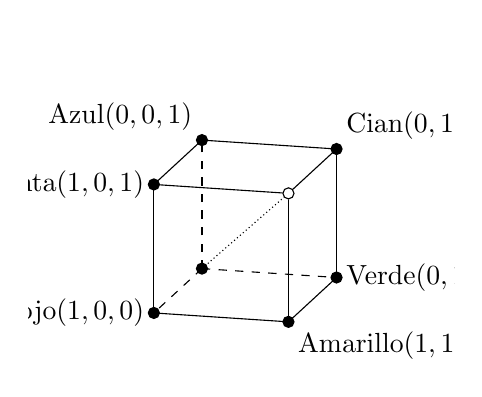
\begin{tikzpicture}
                \begin{axis}[view={105}{15},
                width=7cm,height=7cm,
                xtick=\empty,
                ytick=\empty,
                ztick=\empty,
                xmin=0, xmax=30,
                ymin=-10, ymax=30,
                zmin=-10, zmax=30,
                axis lines=center,
                axis line style={draw=none},
                ticks=none,
                ]
                    \def\radio{16}
                    \draw[dashed] (0,0,0) -- (\radio,0,0) node[left] {\makecell{Rojo \\ $(1, 0, 0)$}};
                    \draw[dashed] (0,0,0) -- (0,\radio,0) node[right] {\makecell{Verde \\ $(0, 1, 0)$}};
                    \draw[dashed] (0,0,0) -- (0,0,\radio) node[above left] {\makecell{Azul \\ $(0, 0, 1)$}};
                    \draw (\radio,0,0) -- (\radio,0,\radio) node[left] {\makecell{Magenta \\ $(1, 0, 1)$}};
                    \draw (\radio,0,0) -- (\radio,\radio,0) node[below right] {\makecell{Amarillo \\ $(1, 1, 0)$}};
                    \draw (\radio,\radio,0) -- (0,\radio,0);
                    \draw (0,\radio,0) -- (0,\radio,\radio) node[above right] {\makecell{Cian \\ $(0, 1, 1)$}};
                    \draw[densely dotted] (0,0,0) -- (\radio,\radio,\radio);
                    \draw (\radio,\radio,0) -- (\radio,\radio,\radio);
                    \draw (0,0,\radio) -- (\radio,0,\radio) -- (\radio,\radio,\radio) -- (0,\radio,\radio) -- cycle;
                    %
                    \filldraw (0,0,0) circle (2pt);
                    \filldraw (\radio,0,0) circle (2pt);
                    \filldraw (\radio,\radio,0) circle (2pt);
                    \filldraw (0,\radio,0) circle (2pt);
                    \filldraw (0,0,\radio) circle (2pt);
                    \filldraw (\radio,0,\radio) circle (2pt);
                    \filldraw (0,\radio,\radio) circle (2pt);
                    \filldraw[white] (\radio,\radio,\radio) circle (2pt);
                    \draw (\radio,\radio,\radio) circle (2pt);
                \end{axis}
            \end{tikzpicture}
            \captionsetup*[figure]{hypcap=false}%
            \captionof{figure}{Representación del espacio de color RGB como un cubo en $\RR[3]$}
            \label{fig:cuboRGB}
        \end{center}
    \end{tcolorbox}
\end{adjustwidth}

\newpage

\begin{examplebox}{}{POLILINEAL}
    Demostrar que los polinomios
    $$1, x, x^2, \dots, x^n$$
    forman un conjunto linealmente independiente en $P_n$.

    \tcblower
    \solucion Por conveniencia, denotemos los polinomios como
    $$\mathbb{p}_0 = 1, \mathbb{p}_1 = x, \mathbb{p}_2 = x^2, \dots, \mathbb{p}_n = x^n.$$
    Debemos demostrar que los únicos coeficientes que satisfacen la ecuación vectorial
    \begin{equation}
        a_0\mathbb{p}_0 + a_1\mathbb{p}_1 + a_2\mathbb{p}_2 + \cdots + a_n\mathbb{p}_n = \mathbb{0} \label{eq:vectorial}
    \end{equation}
    son
    $$a_0 = a_1 = a_2 = \cdots = a_n = 0.$$
    La ecuación \eqref{eq:vectorial} es equivalente a la afirmación de que
    \begin{equation}
        a_0 + a_1x + a_2x^2 + \cdots + a_nx^n = 0 \label{eq:polinomial}
    \end{equation}
    para todo $x \in (-\infty, \infty)$. Por lo tanto, debemos demostrar que esto es cierto si y solo si cada coeficiente en \eqref{eq:polinomial} es igual a cero. Para ver que esto es cierto, recordemos del álgebra que un polinomio no nulo de grado $n$ tiene como máximo $n$ raíces distintas. Así, si alguno de los coeficientes en \eqref{eq:polinomial} no es cero, el lado izquierdo sería un polinomio no nulo con un número infinito de raíces, lo cual es una contradicción. Por lo tanto, la ecuación \eqref{eq:vectorial} solo tiene la solución trivial.
\end{examplebox}

\section{Base y dimensión}

\begin{definicion}{}{}
    Decimos que un conjunto finito de vectores $\{ \mathbb{v}_1, \mathbb{v}_2, \dots, \mathbb{v}_n \}$ es una \emph{base} para un espacio vectorial $V$ si:
    \begin{enumerate}[label=\roman*), topsep=6pt, itemsep=0pt]
        \item $\{ \mathbb{v}_1, \mathbb{v}_2, \dots, \mathbb{v}_n \}$ es linealmente independiente,
        \item $\{ \mathbb{v}_1, \mathbb{v}_2, \dots, \mathbb{v}_n \}$ genera a $V$.
    \end{enumerate}
\end{definicion}

Si se considera una base como la descripción de un sistema de coordenadas para un espacio vectorial $V$ de dimensión finita, entonces la parte (i) de esta definición garantiza que no existe ninguna interrelación entre los vectores base, la parte (ii) garantiza que hay suficientes vectores base para proporcionar coordenadas a todos los vectores en $V$. A continuación, se presentan algunos ejemplos.

\begin{examplebox}{}{}
    Recordemos del ejemplo \ref{examplebox:vectores_unitarios_generaRn} que los vectores unitarios estándar en
    \begin{matrizn}
        \makecell{\includegraphics[page=3]{Externalizacion/C1/MatricesC1.pdf}}
    \end{matrizn}
    generan $\RR[n]$ y del ejemplo \ref{examplebox:vectores_unitarios_liRn}, que son linealmente independientes. Por lo tanto, forman una base para $\RR[n]$ que llamamos \emph{base natural}, \emph{base estándar} o \emph{base canónica} para $\RR[n]$. En particular,
    \begin{matrizn}
        \makecell{\includegraphics[page=4]{Externalizacion/C1/MatricesC1.pdf}}
    \end{matrizn}
    es la base estándar para $\RR[3]$.
\end{examplebox}

\newpage

\begin{examplebox}{}{}
    Demostrar que $\mathcalm{B} = \left\{1, x, x^2, \dots, x^n\right\}$ es una base para el espacio vectorial $P_n$ de polinomios de grado $n$ o menor, que llamamos la \emph{base estándar} de $P_n$.
    
    \tcblower
    \solucion Debemos demostrar que los polinomios en $\mathcalm{B}$ son linealmente independientes y generan $P_n$. Denotemos estos polinomios como
    $$\mathbb{p}_0 = 1, \mathbb{p}_1 = x, \mathbb{p}_2 = x^2, \dots, \mathbb{p}_n = x^n.$$
    Mostramos en el ejemplo \ref{examplebox:POLIGENERA} que estos vectores generan $P_n$ y en el ejemplo \ref{examplebox:POLILINEAL} que son linealmente independientes. Por lo tanto, forman una base para $P_n$.
\end{examplebox}

\begin{examplebox}{}{}
    Consideremos el espacio vectorial $\RR[3]$ y el conjunto
    \begin{matrizn}
        \makecell{\includegraphics[page=13]{Externalizacion/C1/MatricesC1.pdf}}
    \end{matrizn}
    Queremos demostrar que este conjunto es una base de $\RR[3]$. Para verificar que $\mathcalm{B}$ es linealmente independiente, formamos la ecuación
    \begin{matrizn}
        \makecell{\includegraphics[page=14]{Externalizacion/C1/MatricesC1.pdf}}
    \end{matrizn}
    y resolvemos para $c_1$, $c_2$, $c_3$. De lo anterior, obtenemos el siguiente sistema lineal
    \begin{align*}
        c_1 + c_3 & = 0 \\
        c_1 + c_2 & = 0 \\
        c_2 + c_3 & = 0
    \end{align*}
    que tiene como única solución $c_1 = c_2 = c_3 = c_4 = 0$, lo cual muestra que $\mathcalm{B}$ es linealmente independiente. Para mostrar que $\mathcalm{B}$ genera a $\RR[3]$, debemos probar que cualquier vector en $\RR[3]$ se puede expresar como combinación lineal de $\mathcalm{B}$, es decir, debemos encontrar constantes $c_1$, $c_2$, $c_3$ tales que
    \begin{matrizn}
        \makecell{\includegraphics[page=15]{Externalizacion/C1/MatricesC1.pdf}}
    \end{matrizn}
    De la expresión anterior, obtenemos el siguiente sistema lineal
    \begin{align*}
        c_1 + c_3 & = x \\
        c_1 + c_2 & = y \\
        c_2 + c_3 & = z
    \end{align*}
    que tiene como única solución
    $$c_1 = \frac{x + y - z}{2}, \quad c_2 = - \frac{x - y - z}{2}, \quad c_3 = \frac{x - y + z}{2}.$$
    Por lo tanto, $\mathcalm{B}$ genera a $\RR[3]$. Se concluye así que $\mathcalm{B}$ es una base para $\RR[3]$.
\end{examplebox}

\begin{examplebox}{}{}
    Determine una base para el subespacio de $P_2$, formado por los vectores de la forma $at^2 + bt + c$ donde $c = a - b$.

    \tcblower
    \solucion Todo vector en $V$ es de la forma
    $$at^2 + bt + a - b,$$
    que puede escribirse como
    $$a(t^2 + 1) + b(t - 1),$$
    \newpage
    lo cual muestra que los vectores $t^2 + 1$ y $t - 1$ generan a $V$. Además, estos vectores son linealmente independientes ya que ninguno es múltiplo del otro. También podría haberse obtenido (con mayor trabajo) esta conclusión sobre independencia lineal, escribiendo la ecuación
    $$a_1(t^2 + 1) + a_2(t - 1) = 0$$
    o
    $$t^2 a_1 + t a_2 + (a_1 - a_2) = 0.$$
    Como esta ecuación se cumple para todos los valores de $t$, debemos tener $a_1 = 0$ y $a_2 = 0$, que es la condición de independencia lineal.
\end{examplebox}

\begin{definicion}{}{}
    Sea $V$ un espacio vectorial sobre $K$. Se llama \emph{dimensión} del espacio vectorial $V$, a la cardinalidad de la base de $V$, y se denotará por $\Dim V$.
\end{definicion}

Un espacio vectorial es de \emph{dimensión finita} si existe un subconjunto finito de $V$ que es una base para $V$; en caso contrario, es decir, si no existe tal subconjunto finito, el espacio es de \emph{dimensión infinita}.

Casi todos los espacios vectoriales considerados en este libro son de dimensión finita. Sin embargo, es conveniente anotar que muchos espacios vectoriales de importancia en matemáticas y en física son de dimensión infinita; su estudio excede el alcance de este libro. El espacio vectorial $P$, de todos los polinomios, y el espacio vectorial $C(-\infty, \infty)$ de las funciones continuas $f: \RR \longrightarrow \RR$, no son de dimensión finita.

Ahora estableceremos algunos resultados relativos a espacios vectoriales de dimensión finita, que hacen referencia al número de vectores en una base, comparan el número de vectores de dos bases diferentes y establecen propiedades de las bases.

\begin{theorem}{}{}
    Sea $V$ un espacio vectorial y sea $\mathcalm{B} = \{ \mathbb{v}_1, \mathbb{v}_2, \dots, \mathbb{v}_n \}$ una base de $V$. Entonces todo elemento de $V$ se expresa de manera única a partir de los elementos de la base. Es decir, dado $\mathbb{u} \in V$, existen escalares $a_1$, $a_2$, $\dots$, $a_n$ únicos tales que
    \begin{equation}
        \mathbb{u} = a_1\mathbb{v}_1 + a_2\mathbb{v}_2 + \cdots + a_n\mathbb{v}_n \label{ec25}
    \end{equation}

    \tcblower
    \demostracion Supongamos que existen escalares $b_1$, $b_2$, $\dots$, $b_n$ tales que
    \begin{equation}
        \mathbb{u} = b_1\mathbb{v}_1 + b_2\mathbb{v}_2 + \cdots + b_n\mathbb{v}_n \label{ec26}
    \end{equation}
    Se demostrará que $a_i = b_i$, para $i = 1$, $2$, $\dots$, $n$. Sea
    \begin{align*}
        -\mathbb{u} & = (-1) \cdot \mathbb{u} \\
        & = (-1) \cdot (b_1\mathbb{v}_1 + b_2\mathbb{v}_2 + \cdots + b_n\mathbb{v}_n) \\
        & = (-1)b_1\mathbb{v}_1 + (-1)b_2\mathbb{v}_2 + \cdots + (-1)b_n\mathbb{v}_n \\
        & = (-b_1)\mathbb{v}_1 + (-b_2)\mathbb{v}_2 + \cdots + (-b_n)\mathbb{v}_n
    \end{align*}
    Ahora, de las expresiones \eqref{ec25} y \eqref{ec26} tenemos
    \begin{align*}
        \mathbb{0} & = \mathbb{u} + (-\mathbb{u}) \\
        & = a_1\mathbb{v}_1 + a_2\mathbb{v}_2 + \cdots + a_n\mathbb{v}_n + (-b_1)\mathbb{v}_1 + (-b_2)\mathbb{v}_2 + \cdots + (-b_n)\mathbb{v}_n \\
        & = \big(a_1+(-b_1)\big)\mathbb{v}_1 + \big(a_2+(-b_2)\big)\mathbb{v}_2 + \cdots + \big(a_n+(-b_n)\big)\mathbb{v}_n
    \end{align*}
    Como $\mathcalm{B}$ es linealmente independiente,
    $$\big(a_1+(-b_1)\big) = 0, \big(a_2+(-b_2)\big) = 0, \dots, \big(a_n+(-b_n)\big) = 0,$$
    de modo que $b_1 = a_1$, $b_2 = a_2$, $\dots$, $b_n = a_n$. Por lo tanto, solo hay una forma de expresar $\mathbb{u}$ como combinación lineal de los vectores en $\mathcalm{B}$.
\end{theorem}

\newpage

Supongamos que $\mathcalm{B} = \{\mathbb{v}_1, \mathbb{v}_2, \dots, \mathbb{v}_n\}$ genera un espacio vectorial $V$ y que $\mathbb{v}_j$ es una combinación lineal de los vectores que le preceden en $\mathcalm{B}$. Entonces el conjunto
$$\mathcalm{A} = \{\mathbb{v}_1, \mathbb{v}_2, \dots, \mathbb{v}_{j-1}, \mathbb{v}_{j+1}, \dots, \mathbb{v}_n\}$$
que consta de los vectores en $\mathcalm{B}$, con excepción de $\mathbb{v}_j$, también genera a $V$. Para demostrar este resultado, observemos que si $\mathbb{v}$ es cualquier vector en $V$, entonces, como $\mathcalm{B}$ genera a $V$, podemos encontrar escalares $a_1$, $a_2$, $\dots$, $a_n$ tales que
$$\mathbb{v} = a_1 \mathbb{v}_1 + a_2 \mathbb{v}_2 + \cdots + a_{j-1} \mathbb{v}_{j-1} + a_j \mathbb{v}_j + a_{j+1} \mathbb{v}_{j+1} + \cdots + a_n \mathbb{v}_n.$$
Ahora, si
$$\mathbb{v}_j = b_1 \mathbb{v}_1 + b_2 \mathbb{v}_2 + \cdots + b_{j-1} \mathbb{v}_{j-1},$$
entonces
\begin{align*}
    \mathbb{v} & = a_1 \mathbb{v}_1 + a_2 \mathbb{v}_2 + \cdots + a_{j-1} \mathbb{v}_{j-1} + a_j (b_1 \mathbb{v}_1 + b_2 \mathbb{v}_2 + \cdots + b_{j-1} \mathbb{v}_{j-1}) \\
    & \hspace{3cm} + a_{j+1} \mathbb{v}_{j+1} + \cdots + a_n \mathbb{v}_n \\
    & = c_1 \mathbb{v}_1 + c_2 \mathbb{v}_2 + \cdots + c_{j-1} \mathbb{v}_{j-1} + c_{j+1} \mathbb{v}_{j+1} + \cdots + c_n \mathbb{v}_n
\end{align*}
lo cual significa que $\Gen \mathcalm{A} = V$.

\begin{theorem}{}{algunsubbW}
    Sea $\mathcalm{B} = \{\mathbb{v}_1, \mathbb{v}_2, \dots, \mathbb{v}_n\}$ un conjunto de vectores no nulos en un espacio vectorial $V$ y sea $W = \Gen \mathcalm{B}$. Entonces, algún subconjunto de $\mathcalm{B}$ es una base para $W$.

    \tcblower
    \demostracion Procedamos por casos.
    \begin{enumerate}[label=\roman*), topsep=6pt, itemsep=0pt]
        \item Si $\mathcalm{B}$ es linealmente independiente, entonces $\mathcalm{B}$ es una base para $W$ porque $\mathcalm{B}$ es generador de $W$, de acuerdo con la hipótesis.
        \item Si $\mathcalm{B}$ es linealmente dependiente, entonces existen $c_1, c_2, \dots, c_n$, no todos iguales a cero, tales que
        $$c_1 \mathbb{v}_1 + c_2 \mathbb{v}_2 + \cdots + c_n \mathbb{v}_n = \mathbb{0}.$$
        Por lo tanto, algún $\mathbb{v}_j$ es una combinación lineal de los vectores anteriores en $\mathcalm{B}$ (teorema \ref{theorem:licombinacion_lineal}). Ahora, eliminamos $\mathbb{v}_j$ de $\mathcalm{B}$, para obtener un subconjunto $\mathcalm{B}_1$ de $\mathcalm{B}$. Entonces, por la observación anterior a este teorema, concluimos que $\mathcalm{B}_1 = \{\mathbb{v}_1, \mathbb{v}_2, \dots, \mathbb{v}_{j-1}, \mathbb{v}_{j+1}, \dots, \mathbb{v}_n\}$ genera a $W$. Si $\mathcalm{B}_1$ es linealmente independiente, entonces $\mathcalm{B}_1$ es una base. Si $\mathcalm{B}_1$ es linealmente dependiente, eliminamos un vector de $\mathcalm{B}_1$ que sea combinación lineal de los vectores que le preceden en $\mathcalm{B}_1$ y obtenemos un nuevo conjunto $\mathcalm{B}_2$ que también genera a $W$. Continuando de esta forma, y dado que $\mathcalm{B}$ es un conjunto finito, en algún momento encontraremos un subconjunto $\mathcalm{A}$ de $\mathcalm{B}$ que es linealmente independiente y genera a $W$. Tal conjunto $\mathcalm{A}$ es una base para $W$.
    \end{enumerate}
\end{theorem}

\begin{examplebox}{}{}
    La dimensión de $\RR[2]$ es $2$; la dimensión de $\RR[3]$ es $3$; y en general, la dimensión de $\RR[n]$ es $n$. Esto se expresa respectivamente como $\Dim \RR[2] = 2$, $\Dim \RR[3] = 3$, $\Dim \RR[n] = n$.
\end{examplebox}

\begin{examplebox}{}{}
    La dimensión de $P_2$ es $3$; la dimensión de $P_3$ es $4$; y en general, la dimensión de $P_n$ es $n + 1$. Esto se expresa respectivamente como $\Dim P_2 = 3$, $\Dim P_3 = 4$, $\Dim P_n = n + 1$.
\end{examplebox}

\begin{examplebox}{}{}
    Si $\mathcalm{B} = \{\mathbb{v}_1, \mathbb{v}_2, \dots, \mathbb{v}_r\}$, entonces cada vector en $\Gen \mathcalm{B}$ se puede expresar como una combinación lineal de los vectores en $\mathcalm{B}$. Así, si los vectores en $\mathcalm{B}$ son linealmente independientes, automáticamente forman una base para $\Gen \mathcalm{B}$, de lo cual podemos concluir que
    $$\Dim \Gen(\{\mathbb{v}_1, \mathbb{v}_2, \dots, \mathbb{v}_r\}) = r.$$
    En otras palabras, la dimensión del espacio generado por un conjunto linealmente independiente de vectores es igual al número de vectores en ese conjunto.
\end{examplebox}

\newpage

Observemos que si $\{ \mathbb{v}_1, \mathbb{v}_2, \dots, \mathbb{v}_n \}$ es una base para un espacio vectorial $V$, entonces $\{ c\mathbb{v}_1, c\mathbb{v}_2, \dots, c\mathbb{v}_n \}$ también es una base, si $c \neq 0$. Esta observación muestra que un espacio vectorial real diferente de $\mathbb{0}$ tiene siempre infinitas bases.

\begin{theorem}{}{vmenorli}
    Sea $V$ un espacio vectorial de dimensión finita. Si $\mathcalm{B} = \{\mathbb{v}_1, \mathbb{v}_2, \dots, \mathbb{v}_n\}$ es una base para $V$ y $\mathcalm{A} = \{\mathbb{w}_1, \mathbb{w}_2, \dots, \mathbb{w}_r\}$ es un conjunto linealmente independiente de vectores en $V$, entonces $r \leq n$.

    \tcblower
    \demostracion Sea $\mathcalm{A}_1 = \{\mathbb{w}_1, \mathbb{v}_1, \mathbb{v}_2, \dots, \mathbb{v}_n\}$. Como $\mathcalm{B}$ genera a $V$, $\mathcalm{A}_1$ también lo genera. Y, puesto que $\mathbb{w}_1$ es una combinación lineal de los vectores de $\mathcalm{B}$, $\mathcalm{A}_1$ es linealmente dependiente. Entonces, de acuerdo con el teorema \ref{theorem:licombinacion_lineal}, algún $\mathbb{v}_j$ es una combinación lineal de los vectores que le preceden en $\mathcalm{A}_1$. Eliminemos ese vector particular $\mathbb{v}_j$. Sea $\mathcalm{B}_1 = \{\mathbb{w}_1, \mathbb{v}_1, \dots, \mathbb{v}_{j-1}, \mathbb{v}_{j+1}, \dots, \mathbb{v}_n\}$. Observemos que $\mathcalm{B}_1$ genera a $V$. A continuación, sea $\mathcalm{A}_2 = \{\mathbb{w}_2, \mathbb{w}_1, \mathbb{v}_1, \dots, \mathbb{v}_{j-1}, \mathbb{v}_{j+1}, \dots, \mathbb{v}_n\}$. Entonces $\mathcalm{A}_2$ es linealmente dependiente, y algún vector en $\mathcalm{A}_2$ es una combinación lineal de los vectores precedentes en $\mathcalm{A}_2$. Como $\mathcalm{A}$ es linealmente independiente, dicho vector no puede ser $\mathbb{w}_1$, así que es $\mathbb{v}_i$, con $i \neq j$. Repetimos este proceso una y otra vez. Si se eliminan todos los vectores $\mathbb{v}$ antes de que se puedan incluir todos los vectores $\mathbb{w}$, entonces el conjunto resultante de vectores $\mathbb{w}$, un subconjunto de $\mathcalm{A}$, es linealmente dependiente, lo cual implica que también $\mathcalm{A}$ es linealmente dependiente. Esta contradicción permite concluir que el número $r$ de vectores $\mathbb{w}$ no puede ser mayor que el número $n$ de vectores $\mathbb{v}$. Esto es, $r \leq n$.
\end{theorem}

\begin{corollary}{}{}
    Si $\mathcalm{B} = \{\mathbb{v}_1, \mathbb{v}_2, \dots, \mathbb{v}_n\}$ y $\mathcalm{A} = \{\mathbb{w}_1, \mathbb{w}_2, \dots, \mathbb{w}_m\}$ son dos bases para un espacio vectorial, entonces $n = m$.

    \tcblower
    \demostracion Como $\mathcalm{A}$ es un conjunto linealmente independiente de vectores, el teorema \ref{theorem:vmenorli} implica que $m \leq n$. Igualmente, tenemos que $n \leq m$, puesto que $\mathcalm{B}$ es linealmente independiente. Entonces, $n = m$.
\end{corollary}

Se puede probar que todos los espacios de dimensión finita que tienen igual dimensión difieren solo en la naturaleza de sus elementos; sus propiedades algebraicas son idénticas.

A continuación, enunciaremos una consecuencia directa del teorema \ref{theorem:vmenorli}.

\begin{theorem}{}{}
    Sea $V$ un espacio vectorial de dimensión finita $n$, y sea $W$ un subespacio no nulo de $V$, entonces $\Dim W \leq \Dim V$.

    \tcblower
    \demostracion Sea $\{ \mathbb{v}_1, \mathbb{v}_2, \dots, \mathbb{v}_k \}$ una base de $W$. Al ser una base, los vectores $\mathbb{v}_1, \mathbb{v}_2, \dots, \mathbb{v}_k$ son linealmente independientes. Por el teorema \ref{theorem:vmenorli}, sabemos que $k \leq n$, de donde se sigue que
    $$\Dim W = k \leq n = \Dim V.$$
    Por lo tanto, $\Dim W \leq \Dim V$.
\end{theorem}

En la observación anterior al teorema \ref{theorem:vmenorli} mencionamos que un espacio vectorial tiene muchas bases; pero acabamos de demostrar que, para un espacio vectorial particular $V$, todas las bases tienen el mismo número de vectores. Este hecho conduce a la propia definición de dimensión.

Se puede probar que si un espacio vectorial $V$ tiene dimensión finita $n$, entonces cualquier conjunto de $n + 1$ vectores en $V$ es linealmente dependiente. En particular, cualquier conjunto con más de $n$ vectores en $\RR[n]$ es linealmente dependiente (teorema \ref{theorem:Rnldsinmm}. A continuación, demostraremos que si $\Dim V = n$, entonces ningún conjunto de $n - 1$ vectores en $V$ puede generar a $V$. Por ejemplo, sabemos que la dimensión de $P_2$ es $3$. Entonces el conjunto $\left\{ 1 - x^2, x \right\}$ no puede ser una base de $P_2$, pues tendríamos a lo más dos vectores linealmente independientes y $2 < 3 = \Dim P_2$.

\newpage

\begin{theorem}{}{}
    Si $V$ es un espacio vectorial de dimensión finita $n$, entonces ningún conjunto con $n - 1$ vectores de $V$ puede generar a $V$.

    \tcblower
    \demostracion Sea $V$ un espacio vectorial de dimensión finita $n$. Supongamos que $\mathcalm{B} = \{\mathbb{v}_1, \mathbb{v}_2, \dots, \mathbb{v}_{n-1}\}$ es subconjunto de $V$ y que además, $\mathcalm{B}$ genera $V$. Entonces, por el teorema \ref{theorem:algunsubbW} existe un subconjunto $\mathcalm{B}_1$ de $\mathcalm{B}$ tal que $\mathcalm{B}_1$ es una base de $V$. Dado que $\mathcalm{B}_1$ es una base de $V$, tenemos que
    \begin{equation}
        \Dim V = |\mathcalm{B}_1|. \label{IAOQPOQIQI}
    \end{equation}
    Como $\mathcalm{B}_1$ es subconjunto de $\mathcalm{B}$, se cumple que
    \begin{equation}
        |\mathcalm{B}_1| \leq |\mathcalm{B}| = n - 1. \label{AOPAPOBCCA}
    \end{equation}
    Las ecuaciones \eqref{IAOQPOQIQI} y \eqref{AOPAPOBCCA} juntas implican que
    $$\Dim V \leq n - 1 $$
    lo cual es una contradicción con la hipótesis de que $\Dim V = n$. Por lo tanto, $\mathcalm{B}$ no puede generar $V$.
\end{theorem}

De acuerdo con la definición, un conjunto de vectores en un espacio vectorial $V$ es una base para $V$ si genera a $V$ y es linealmente independiente. Sin embargo, si sabemos que la dimensión de $V$ es $n$, y el conjunto tiene $n$ vectores, solo necesitamos verificar una de las dos condiciones, de acuerdo con el siguiente teorema.

\begin{theorem}{}{siLIByGB}
    Sea $V$ un espacio vectorial de dimensión $n$ y sea $\mathcalm{B} = \{\mathbb{v}_1, \mathbb{v}_2, \dots, \mathbb{v}_n\}$ un conjunto de $n$ vectores en $V$.
    \begin{enumerate}[label=\roman*), topsep=6pt, itemsep=0pt]
        \item Si $\mathcalm{B}$ es linealmente independiente, entonces es una base para $V$.
        \item Si $\mathcalm{B}$ genera a $V$, entonces es una base para $V$.
    \end{enumerate}

    \tcblower
    \demostracion
    \begin{enumerate}[label=\roman*), topsep=6pt, itemsep=0pt]
        \item Dado que $\mathcalm{B}$ es linealmente independiente y $\dim V = n$, entonces existe una base $\mathcalm{A}$ para $V$, que contiene a $\mathcalm{B}$. Pero, dado que $\dim V = n$, $\mathcalm{A}$ no puede contener más elementos que $\mathcalm{B}$. Esto implica que $\mathcalm{B} = \mathcalm{A}$. Por lo tanto, $\mathcalm{B}$ es una base de $V$.
        \item Dado que $\mathcalm{B}$ genera $V$, podemos decir que algún subconjunto de $\mathcalm{B}$, digamos $\mathcalm{A}$, es una base de $V$. Como $\dim V = n$, el conjunto $\mathcalm{A}$ contiene exactamente $n$ elementos. Esto implica que $\mathcalm{B} = \mathcalm{A}$. Por lo tanto, $\mathcalm{B}$ es una base de $V$.
    \end{enumerate}
\end{theorem}

A continuación enunciaremos un teorema para construir una base que contenga un conjunto dado de vectores linealmente independientes.

\begin{theorem}{}{}
    Si $\mathcalm{A}$ es un conjunto de vectores linealmente independientes en un espacio vectorial de dimensión finita $V$, existe una base $\mathcalm{B}$ para $V$, que contiene a $\mathcalm{A}$.

    \tcblower
    \demostracion Sea $\mathcalm{A} = \{ \mathbb{v}_1, \mathbb{v}_2, \dots, \mathbb{v}_k \}$ un conjunto de vectores linealmente independientes en $V$, donde $k \leq n$. Como $V$ es de dimensión finita $n$, sabemos que existe una base $\mathcalm{B} = \{ \mathbb{v}_1, \mathbb{v}_2, \dots, \mathbb{v}_k, \mathbb{w}_1, \mathbb{w}_2, \dots, \mathbb{w}_{n-k} \}$ de $V$, donde los $\mathbb{w}_i$ son vectores adicionales que completan la base. Entonces, el conjunto $\mathcalm{B}$ genera a $V$. Ahora bien, queremos demostrar que $\mathcalm{A} \cup \{\mathbb{w}_1, \mathbb{w}_2, \dots, \mathbb{w}_{n-k}\}$ es un conjunto de vectores linealmente independientes. Es decir, debemos demostrar que
    $$c_1 \mathbb{v}_1 + c_2 \mathbb{v}_2 + \dots + c_k \mathbb{v}_k + d_1 \mathbb{w}_1 + d_2 \mathbb{w}_2 + \dots + d_{n-k} \mathbb{w}_{n-k} = 0.$$
    tiene como solución la trivial. Pero, $\mathcalm{A}$ es linealmente independiente, por lo que
    $$c_1 = c_2 = \dots = c_k = 0.$$
    \newpage
    Por lo tanto, la ecuación se reduce a
    $$d_1 \mathbb{w}_1 + d_2 \mathbb{w}_2 + \dots + d_{n-k} \mathbb{w}_{n-k} = 0.$$
    Como $\{ \mathbb{w}_1, \mathbb{w}_2, \dots, \mathbb{w}_{n-k} \}$ son parte de la base de $V$, también son linealmente independientes, lo que implica que
    $$d_1 = d_2 = \dots = d_{n-k} = 0.$$
	Esto demuestra que el conjunto $\{ \mathbb{v}_1, \mathbb{v}_2, \dots, \mathbb{v}_k, \mathbb{w}_1, \mathbb{w}_2, \dots, \mathbb{w}_{n-k} \}$ es linealmente independiente. Como el conjunto $\mathcalm{A} \cup \{ \mathbb{w}_1, \mathbb{w}_2, \dots, \mathbb{w}_{n-k} \}$ es linealmente independiente y tiene $n$ vectores, entonces este conjunto es una base de $V$.
\end{theorem}

El teorema anterior establece que un conjunto linealmente independiente de vectores en un espacio vectorial $V$ puede extenderse a una base para $V$.

\begin{examplebox}{}{}
    Sea $V = \RR[3]$ y sea el conjunto de vectores $\mathcalm{A} = \{ \mathbb{v}_1, \mathbb{v}_2 \}$, donde
    \begin{matrizn}
        \makecell{\includegraphics[page=16]{Externalizacion/C1/MatricesC1.pdf}}
    \end{matrizn}
    Queremos demostrar que existe una base $\mathcalm{B}$ para $V$ que contenga a $\mathcalm{A}$. Notemos que $\mathcalm{A}$ es linealmente independiente, ya que no existe un escalar $c$ tal que $c\mathbb{v}_1 = \mathbb{v}_2$. Aunque $\mathcalm{A}$ es linealmente independiente en $\RR[3]$, no contiene tres vectores. Como $\RR[3]$ tiene dimensión 3, necesitamos agregar un tercer vector a $\mathcalm{A}$ para completar la base de $V$. Podemos elegir un tercer vector, por ejemplo,
    \begin{matrizn}
        \makecell{\includegraphics[page=17]{Externalizacion/C1/MatricesC1.pdf}}
    \end{matrizn}
    que no es combinación lineal de los vectores en $\mathcalm{A}$. Ahora, debemos verificar que
    $$\mathcalm{B} = \{ \mathbb{v}_1, \mathbb{v}_2, \mathbb{v}_3 \}$$
    es linealmente independiente, pero este es linealmente independiente ya que ninguno de estos vectores puede escribirse como una combinación lineal de los otros. Además, $\mathcalm{B}$ genera $\RR[3]$, porque cualquier vector en $\RR[3]$ puede escribirse como una combinación lineal de estos tres vectores. Es decir,
    \begin{matrizn}
        \makecell{\includegraphics[page=18]{Externalizacion/C1/MatricesC1.pdf}}
    \end{matrizn}
    cuya solución es
    $$c_1 = y, \quad c_2 = x - y, \quad c_3 = -x + y + z.$$
    Por lo tanto, $\mathcalm{B}$ es una base para $\RR[3]$ y contiene al conjunto $\mathcalm{A}$.
\end{examplebox}

Recordemos que la dimensión de un espacio vectorial se define como la cantidad de vectores linealmente independientes necesarios para generar todo el espacio. En el caso del vector cero, su dimensión es $0$ porque no puede generar ningún otro vector aparte de sí mismo mediante combinaciones lineales. Para entenderlo mejor, consideremos que cualquier vector $\mathbb{v}$ en un espacio vectorial $V$ puede ser expresado como
$$\mathbb{v} = c_1 \mathbb{v}_1 + c_2 \mathbb{v}_2 + \cdots + c_n \mathbb{v}_n$$
donde $\mathbb{v}_1, \mathbb{v}_2, \dots, \mathbb{v}_n$ son vectores linealmente independientes en $V$, y $c_1, c_2, \dots, c_n$ son escalares. Ahora, si consideramos el vector cero, no importa cuánto intentemos expresarlo como una combinación lineal de otros vectores $\mathbb{v}_1, \mathbb{v}_2, \dots, \mathbb{v}_n$, siempre obtendremos $\mathbb{0}$ como resultado, ya que cualquier escalar multiplicado por $\mathbb{0}$ sigue siendo $\mathbb{0}$.

\newpage

\begin{theorem}{}{dimSumadeSEV}
    Sea $V$ un espacio vectorial de dimensión finita $n$. Si $S$ y $T$ son subespacios de $V$, entonces
    $$\Dim (S + T) = \Dim(S) + \Dim(T) - \Dim(S \cap T).$$

    \tcblower
    \demostracion Como $S$ y $T$ son subespacios de $V$, entonces $S + T$ y $S \cap T$ son subespacios de $V$ (por el ejercicio \ref{ejercicio_sumadesubs}, pág. \pageref{ejercicio_sumadesubs} y teorema \ref{theorem:intersubsV}). Además, como $V$ es de dimensión finita, entonces $S$, $T$, $S + T$ y $S \cap T$ son de dimensión finita. Sean
    $$\dim S = r, \quad \dim T = m, \quad \dim (S \cap T) = k.$$
    Sea
    $$\{\mathbb{u}_1, \mathbb{u}_2, \dots, \mathbb{u}_k\}$$
    una base de $S \cap T$. Claro que $\{\mathbb{u}_1, \mathbb{u}_2, \dots, \mathbb{u}_k\} \subset S$ es linealmente independiente y podemos completarlo con $\mathbb{v}_1, \mathbb{v}_2, \dots, \mathbb{v}_{r-k} \in S$ a una base de $S$, y por tanto
    $$\{\mathbb{u}_1, \mathbb{u}_2, \dots, \mathbb{u}_k, \mathbb{v}_1, \mathbb{v}_2, \dots, \mathbb{v}_{r-k}\}$$
    es una base de $S$. Análogamente, $\{\mathbb{u}_1, \mathbb{u}_2, \dots, \mathbb{u}_k\} \subset T$ es linealmente independiente y podemos completarlo con $\mathbb{w}_1, \mathbb{w}_2, \dots, \mathbb{w}_{m-k} \in T$ a una base de $T$, y por tanto
    $$\{\mathbb{u}_1, \mathbb{u}_2, \dots, \mathbb{u}_k, \mathbb{w}_1, \mathbb{w}_2, \dots, \mathbb{w}_{m-k}\}$$
    es una base de $T$. Probaremos enseguida que
    $$\mathcalm{B} = \{\mathbb{v}_1, \mathbb{v}_2, \dots, \mathbb{v}_{r-k}, \mathbb{u}_1, \mathbb{u}_2, \dots, \mathbb{u}_k, \mathbb{w}_1, \mathbb{w}_2, \dots, \mathbb{w}_{m-k}\}$$
    es una base de $S + T$. Primero, demostremos que, en efecto, $\mathcalm{B}$ genera a $S + T$. Sea $\mathbb{s} \in S + T$, entonces $\mathbb{s} = \mathbb{u} + \mathbb{v}$. Es decir, existen $s_1, \dots, s_k, b_1, \dots, b_{r-k}$ y $t_1, \dots, t_k, a_1, \dots, a_{m-k}$ escalares tales que
    $$\mathbb{u} = s_1 \mathbb{u}_1 + \cdots + s_k \mathbb{u}_k + b_1 \mathbb{v}_1 + \cdots + b_{r-k} \mathbb{v}_{r-k}$$
    y
    $$\mathbb{v} = t_1 \mathbb{u}_1 + \cdots + t_k \mathbb{u}_k + a_1 \mathbb{w}_1 + \cdots + a_{m-k} \mathbb{w}_{m-k}.$$
    Lo que nos lleva a que
    $$\mathbb{s} = b_1 \mathbb{v}_1 + \cdots + b_{r-k} \mathbb{v}_{r-k} + (s_1 + t_1)\mathbb{u}_1 + \cdots + (s_k + t_k)\mathbb{u}_k + a_1 \mathbb{w}_1 + \cdots + a_{m-k} \mathbb{w}_{m-k}.$$
    Por lo tanto, $\mathbb{s} \in \Gen (\{\mathbb{v}_1, \dots, \mathbb{v}_{r-k}, \mathbb{u}_1, \dots, \mathbb{u}_k, \mathbb{w}_1, \dots, \mathbb{w}_{m-k}\})$, lo que implica que $\mathcalm{B}$ genera a $S + T$. Ahora, demostremos que, en efecto, $\mathcalm{B}$ es linealmente independiente. Sean $x_1, \dots, x_{r-k}, y_1, \dots, y_k, z_1, \dots, z_{m-k}$ escalares tales que
    $$0 = x_1 \mathbb{v}_1 + \dots + x_{r-k} \mathbb{v}_{r-k} + y_1 \mathbb{u}_1 + \dots + y_k \mathbb{u}_k + z_1 \mathbb{w}_1 + \dots + z_{m-k} \mathbb{w}_{m-k}.$$
    Entonces
    $$x_1 \mathbb{v}_1 + \dots + x_{r-k} \mathbb{v}_{r-k} = -(y_1 \mathbb{u}_1 + \dots + y_k \mathbb{u}_k + z_1 \mathbb{w}_1 + \dots + z_{m-k} \mathbb{w}_{m-k}),$$
    por tanto
    $$x_1 \mathbb{v}_1 + \dots + x_{r-k} \mathbb{v}_{r-k} \in T.$$
    Como
    $$x_1 \mathbb{v}_1 + \dots + x_{r-k} \mathbb{v}_{r-k} \in S,$$
    entonces
    $$x_1 \mathbb{v}_1 + \dots + x_{r-k} \mathbb{v}_{r-k} \in S \cap T.$$
    Por tanto existen $c_1, \dots, c_k$ escalares tales que
    $$x_1 \mathbb{v}_1 + \dots + x_{r-k} \mathbb{v}_{r-k} = c_1 \mathbb{u}_1 + \dots + c_k \mathbb{u}_k.$$
    Consecuentemente
    $$y_1 \mathbb{u}_1 + \dots + y_k \mathbb{u}_k + z_1 \mathbb{w}_1 + \dots + z_{m-k} \mathbb{w}_{m-k} = 0,$$
    \newpage
    y como
    $$\{\mathbb{u}_1, \mathbb{u}_2, \dots, \mathbb{u}_k, \mathbb{w}_1, \mathbb{w}_2, \dots, \mathbb{w}_{m-k}\}$$
    es base de $T$, entonces
    $$0 = y_1 = \dots = y_k = z_1 = \dots = z_{m-k}.$$
    Por tanto
    $$\{\mathbb{v}_1, \mathbb{v}_2, \dots, \mathbb{v}_{r-k}, \mathbb{u}_1, \mathbb{u}_2, \dots, \mathbb{u}_k, \mathbb{w}_1, \mathbb{w}_2, \dots, \mathbb{w}_{m-k}\}$$
    es linealmente independiente. Por todo lo anterior,
    $$\{\mathbb{v}_1, \mathbb{v}_2, \dots, \mathbb{v}_{r-k}, \mathbb{u}_1, \mathbb{u}_2, \dots, \mathbb{u}_k, \mathbb{w}_1, \mathbb{w}_2, \dots, \mathbb{w}_{m-k}\}$$
    es base de $S + T$, entonces
    \begin{align*}
        \dim(S + T) & = (r - k) + k + (m - k) \\
        & = r + m - k \\
        & = \dim S + \dim T - \dim(S \cap T)
    \end{align*}
\end{theorem}

\begin{examplebox}{}{}
    En $P_3$, sean
    $$W_1 = \left\{ p(x) \in P_3 \text{ tal que } x^2 - 1 \mid p(x) \right\}$$
    y
    $$W_2 = \left\{ p(x) \in P_3 \text{ tal que } x^2 + x - 2 \mid p(x) \right\}.$$
    Obtenga una base y la dimensión de los siguientes subespacios:
    \begin{tasks}(4)
        \task $W_1$,
        \task $W_2$,
        \task $W_1 \cap W_2$,
        \task $W_1 + W_2$.
    \end{tasks}

    \tcblower
    \demostracion Antes de empezar, recordemos la definición de divisibilidad de polinomios: Sean $f(x)$, $g(x) \in P_n$. Decimos que $g(x)$ divide a $f(x)$, o que $g(x)$ es un factor de $f(x)$, si existe $q(x) \in P_n$ tal que $f(x) = g(x)q(x)$. Comúnmente, para decir que $g(x)$ divide a $f(x)$ se escribe $g(x) \mid f(x)$.
    \begin{enumerate}[label=\alph*), topsep=6pt, itemsep=0pt]
        \item Sea $p(x) \in P_3$, con $p(x) = a_0 + a_1x + a_2x^2 + a_3x^3$, entonces
        \begin{align*}
            p(x) \in W_1 & \Longleftrightarrow x^2 - 1 \mid p(x) \\
            & \Longleftrightarrow \exists q(x) \in P_3 \text{ tal que } p(x) = \left( x^2 - 1 \right) q(x) \\
            & \Longleftrightarrow p(x) = \left( x^2 - 1 \right) (ax + b) \\
            & \Longleftrightarrow p(x) = a\left( x^3 - x \right) + b\left( x^2 - 1 \right)
        \end{align*}
        Por lo tanto, $p(x) \in \Gen \left(\left\{ x^3 - x, x^2 - 1 \right\}\right)$, y como no existe un escalar $c$ tal que $x^2 - 1 = c \left( x^3 - x \right)$, entonces el conjunto $\left\{ x^3 - x, x^2 - 1 \right\}$ es linealmente independiente. Además, es claro que dicho conjunto genera a $W_1$, pues para cualquier escalar $a$ y $b$, $p(x) \in W_1$. Por lo tanto, demostramos que $\mathcalm{A} = \left\{ x^3 - x, x^2 - 1 \right\}$ es una base para $W_1$ y por consiguiente, tenemos que $\Dim W_1 = 2$.
        \item Sea $p(x) \in P_3$, con $p(x) = a_0 + a_1x + a_2x^2 + a_3x^3$, entonces
        \begin{align*}
            p(x) \in W_2 & \Longleftrightarrow x^2 + x - 2 \mid p(x) \\
            & \Longleftrightarrow \exists q(x) \in P_3 \text{ tal que } p(x) = \left( x^2 + x - 2 \right) q(x) \\
            & \Longleftrightarrow p(x) = \left( x^2 + x - 2 \right) (ax + b) \\
            & \Longleftrightarrow p(x) = a\left( x^3 + x^2 - 2x \right) + b\left( x^2 + x - 2 \right)
        \end{align*}
        Por lo tanto, $p(x) \in \Gen \left(\left\{ x^3 + x^2 - 2x, x^2 + x - 2 \right\}\right)$, y como no existe un escalar $c$ tal que $x^3 + x^2 - 2x = c \left( x^2 + x - 2 \right)$, entonces el conjunto $\left\{ x^3 + x^2 - 2x, x^2 + x - 2 \right\}$ es linealmente independiente. Además, es claro que dicho conjunto genera a $W_2$, pues para cualquier $a$ y $b$, $p(x) \in W_2$. Por lo tanto, demostramos que $\mathcalm{B} = \left\{ x^3 + x^2 - 2x, x^2 + x - 2 \right\}$ es una base para $W_2$ y por consiguiente, tenemos que $\Dim W_2 = 2$.
        \item Sea $p(x) \in P_3$, con $p(x) = a_0 + a_1x + a_2x^2 + a_3x^3$, entonces
        \begin{align*}
            p(x) \in W_1 \cap W_2 & \Longleftrightarrow x^2 - 1 \mid p(x) \text{ y } x^2 + x - 2 \mid p(x) \\
            & \Longleftrightarrow (x - 1)(x + 1) \mid p(x) \text{ y } (x - 1)(x + 2) \mid p(x) \\
            & \Longleftrightarrow (x - 1)(x + 1)(x + 2) \mid p(x) \\
            & \Longleftrightarrow c \left( x^3 + 2x^2 - x - 2 \right)
        \end{align*}
        Por lo tanto, $p(x) \in \Gen \left(\left\{ x^3 + 2x^2 - x - 2 \right\}\right)$, y es linealmente independiente, pues es un conjunto de un solo elemento. Además, es claro que dicho conjunto genera a $W_1 \cap W_2$, pues para cualquier escalar $c$, $p(x) \in W_1 \cap W_2$. Por lo tanto, demostramos que $\mathcalm{C} = \left\{ x^3 + 2x^2 - x - 2 \right\}$ es una base de $W_1 \cap W_2$ y por consiguiente, $\Dim (W_1 \cap W_2) = 1$.
        \item Por el ejercicio \ref{ejercicio_sumadesubs} en la página \pageref{ejercicio_sumadesubs}, tenemos que
        \begin{align*}
            W_1 + W_2 & = \Gen(\mathcalm{A} \cup \mathcalm{B}) \\
            & = \Gen \left(\left\{ x^3 - x, x^2 - 1, x^3 + x^2 - 2x, x^2 + x - 2 \right\}\right)
        \end{align*}
        Observemos que
        $$x^2 + x - 2 = \left( x^3 - x \right) + 2\left( x^2 - 1 \right) - \left( x^3 + x^2 - 2x \right).$$
        Por lo tanto, $x^2 + x - 2$ es linealmente dependiente de los otros polinomios y se elimina. Los polinomios restantes forman el conjunto
        $$\mathcalm{D} = \left\{ x^3 - x, x^2 - 1, x^3 + x^2 - 2x \right\}$$
        que es linealmente independiente, pues si formamos la ecuación
        $$a\left(x^3 - x\right) + b\left(x^2 - 1\right) + c\left(x^3 + x^2 - 2x\right) = 0,$$
        que es equivalente a
        $$(a + c)x^3 + (b + c)x^2 + (-a - 2c)x + (-b) = 0,$$
        obtenemos el siguiente sistema lineal
        \begin{align*}
            a + c & = 0 \\
            b + c & = 0 \\
            -a - 2c & = 0 \\
            -b & = 0
        \end{align*}
        que tiene como única solución
        $$a = b = c = 0.$$
        Por el teorema \ref{theorem:dimSumadeSEV} y por los incisos anteriores de este ejemplo,
        \begin{align*}
            \Dim(W_1 + W_2) & = \Dim(W_1) + \Dim(W_2) - \Dim(W_1 \cap W_2) \\
            & = 2 + 2 - 1 = 3
        \end{align*}
        Ahora, sabemos que $\mathcalm{D}$ es linealmente independiente y que además, coincide con la dimensión de $W_1 + W_2$. Así que por el teorema \ref{theorem:siLIByGB}, una base para $W_1 + W_2$ es simplemente $\mathcalm{D} = \left\{ x^3 - x, x^2 - 1, x^3 + x^2 - 2x \right\}$.
    \end{enumerate}
\end{examplebox}

\newpage

\section{Ejercicios del Capítulo 1}

\noindent
De los problemas 1 al 15 determine si el conjunto dado es un espacio vectorial. De no ser así proporcione una lista de los axiomas que no se cumplen.
\begin{enumerate}
    \item El conjunto de números naturales $\NN$ como vectores, el conjunto de números naturales $\NN$ como escalares y la operación de multiplicación para números naturales.
    \item El conjunto de números naturales $\NN$ como vectores, el conjunto de números naturales $\NN$ como escalares, la operación de suma para números naturales y la multiplicación entre números naturales para la operación de multiplicación de escalar y vector.
    \item El conjunto de números enteros $\ZZ$ como vectores, el conjunto de números naturales $\NN$ como escalares, la operación de suma para números enteros y la multiplicación entre números enteros para la operación de multiplicación de escalar y vector.
    \item $\left\{ \begin{pmatrix} x \\ y \end{pmatrix} \mid y \leq 0 \text{ donde } x, y \in \RR \right\}$ con la suma de vectores y multiplicación por un escalar usuales.
    \item Los vectores en el plano que está en el primer cuadrante.
    \item El conjunto de vectores en $\RR[2]$ de la forma $\begin{pmatrix} x \\ x \end{pmatrix}$.
    \item El conjunto de vectores los números racionales $\QQ$ con la operación de suma, el conjunto de escalares los números enteros $\ZZ$ y la operación de multiplicación de escalar y vector la multiplicación usual.
    \item El conjunto de polinomios de grado menor o igual a $n$ con término constante cero.
    \item El conjunto de polinomios de grado menor o igual a $n$ con término constante $a_{0}$ positivo.
    \item El conjunto de polinomios de grado menor o igual a $n$ con término constante $a_{0}$ negativo.
    \item El conjunto de funciones continuas de valores reales definidas en $[0, 1]$ con $f(0) = 0$ y $f(1) = 0$ bajo las operaciones del ejemplo \ref{examplebox:ejemplo5.1.8}.
    \item El conjunto de puntos en $\RR[3]$ que se encuentran sobre una recta que pasa por el origen.
    \item El conjunto de puntos en $\RR[3]$ que se encuentran sobre la recta $x = t+1$, $y = 2t$, $z = t-1$.
    \item El conjunto de funciones diferenciables definidas en $[0, 1]$ con las operaciones del ejemplo \ref{examplebox:ejemplo5.1.8}.
    \item El conjunto de números reales de la forma $a+b \sqrt{2}$, donde $a$ y $b$ son números racionales, bajo la suma de números reales usual y la multiplicación por un escalar definida solo para escalares racionales.
\end{enumerate}
De los problemas 16 al 34 determine si el subconjunto dado $W$ del espacio vectorial $V$ es un subespacio de $V$.
\begin{enumerate}[resume]
    \item $V=\RR[2]$; $W=\left\{ \begin{pmatrix} x \\ y \end{pmatrix} \mid x=3, y \in \RR \right\}$
    \item $V=\RR[2]$; $W=\left\{ \begin{pmatrix} x \\ y \end{pmatrix} \mid y \geq 0 \right\}$\newpage
    \item $V=\RR[2]$; $W=\left\{ \begin{pmatrix} x \\ y \end{pmatrix} \mid x=y \right\}$
    \item $V=\RR[2]$; $W=\left\{ \begin{pmatrix} x \\ y \end{pmatrix} \mid y=2 x \right\}$
    \item $V=\RR[3]$; $W = \operatorname{el~plano} x y$
    \item $V=\RR[2]$; $W=\left\{ \begin{pmatrix} x \\ y \end{pmatrix} \mid x^{2}+y^{2} \leq 1\right\}$
    \item $V=\RR[2]$; $W=\left\{ \begin{pmatrix} x \\ y \end{pmatrix} \mid x^{2}+y^{3}<1\right\}$
    \item $V=\RR$; $W=\QQ$
    \item $V=P_{n}$; $W=\left\{p \in P_{n}\mid p(0)=0\right.$ y $\left.p^{\prime}(0)=0\right\}$
    \item $V=P_{4}$; $W=\left\{p \in P_{4}\mid p(0)=0\right\}$
    \item $V=P_{n}$; $W=\left\{p \in P_{n}\mid p(0)=0\right\}$
    \item $V=P_{n}$; $W=\left\{p \in P_{n}\mid p(0)=1\right\}$
    \item $V=C[0,1]$; $W=\{f \in C[0,1]\mid f(0)=f(1)=0\}$
    \item $V=C[0,1]$; $W=\{f \in C[0,1]\mid f(0)=2\}$
    \item $V=C^{1}[0,1]$; $W=\left\{f \in C^{1}[0,1]\mid f^{\prime}(0)=0\right\}$
    \item $V=C[a, b]$; con $a$, $b \in \RR$ y $a<b$; $\displaystyle W=\left\{f \in C[a, b]\mid \int_{a}^{b} f(x) d x=0\right\}$
    \item $V=C[a, b]$; $\displaystyle W=\left\{f \in C[a, b]\mid \int_{a}^{b} f(x) d x=1\right\}$
    \item $V=C[a, b]$; $\displaystyle W=\left\{f \in C[a, b]\mid \int_{a}^{b} f^{2}(x) d x=0\right\}$
    \item Sea $W=\left\{ \begin{pmatrix} x \\ y \\ z \\ w \end{pmatrix} \mid a x+b y+c z+d w=0\right\}$, donde $a, b, c$ y $d$ son números reales, no todos cero. Demuestre que $W$ es un subespacio propio de $\RR[4]$. $W$ se llama un hiperplano en $\RR[4]$ que pasa por el origen.
\end{enumerate}
De los problemas 35 al 52 determine si el conjunto dado de vectores genera el espacio vectorial dado.
\begin{multienumerate}\setcounter{multienumi}{34}
    \mitemxx{En $ \RR[2]$: $\begin{pmatrix} 2 \\ 10 \end{pmatrix}, \begin{pmatrix} 10 \\ 8 \end{pmatrix}$}{En $ \RR[2]$: $\begin{pmatrix} 1 \\ 2 \end{pmatrix}, \begin{pmatrix} 3 \\ 4 \end{pmatrix}$}
    \mitemxx{En $ \RR[2]$: $\begin{pmatrix} 1 \\ 1 \end{pmatrix}, \begin{pmatrix} 2 \\ 1 \end{pmatrix}, \begin{pmatrix} 2 \\ 2 \end{pmatrix}$}{En $\RR[2]$: $\begin{pmatrix} 0 \\ 1 \end{pmatrix}, \begin{pmatrix} 3 \\ 4 \end{pmatrix}, \begin{pmatrix*}[r] -1 \\ -2 \end{pmatrix*}$}
    \mitemxx{En $ \RR[2]$: $\begin{pmatrix*}[r] -12 \\ 5 \end{pmatrix*}, \begin{pmatrix*}[r] -3 \\ 0 \end{pmatrix*}, \begin{pmatrix*}[r] 4 \\ -8 \end{pmatrix*}$}{En $ \RR[2]$: $\begin{pmatrix} 1 \\ 1 \end{pmatrix}, \begin{pmatrix} 2 \\ 2 \end{pmatrix}, \begin{pmatrix} 5 \\ 5 \end{pmatrix}$}
    \mitemx{En $\RR[2]$: $\begin{pmatrix*}[r] -6 \\ 5 \end{pmatrix*}, \begin{pmatrix} 7 \\ 9 \end{pmatrix}, \begin{pmatrix*}[r] 7 \\ -12 \end{pmatrix*}, \begin{pmatrix*}[r] -10 \\ 6 \end{pmatrix*}$}
    \mitemxx{En $\RR[3]$: $\makecell[l]{\includegraphics[page=19]{Externalizacion/C1/MatricesC1.pdf}}$}{En $\RR[3]$: $\makecell[l]{\includegraphics[page=20]{Externalizacion/C1/MatricesC1.pdf}}$}
    \newpage
    \mitemxx{En $\RR[3]$: $\makecell[l]{\includegraphics[page=21]{Externalizacion/C1/MatricesC1.pdf}}$}{En $\RR[3]$: $\makecell[l]{\includegraphics[page=22]{Externalizacion/C1/MatricesC1.pdf}}$}
    \mitemxx{En $\RR[3]$: $\makecell[l]{\includegraphics[page=23]{Externalizacion/C1/MatricesC1.pdf}}$}{En $ \RR[3]$: $\makecell[l]{\includegraphics[page=24]{Externalizacion/C1/MatricesC1.pdf}}$}
    \mitemxx{En $P_{2}$: $1-x, 3-x^{2}$}{En $P_{2}$: $1-x, 3-x^{2}, x$}
    \mitemx{En $P_{2}$: $x^{2}+1, x^{2}-1, x+6$}
    \mitemx{En $P_{2}$: $-12 x+5 x^{2},-9-27 x+8 x^{2},-3-5 x+x^{2}$}
    \mitemx{En $P_{2}$: $-10+3 x+11 x^{2}, 10+9 x-4 x^{2}, 5+x+4 x^{2}$}
\end{multienumerate}
De los problemas 53 al 60 describa el espacio generado por los vectores.
\begin{multienumerate}\setcounter{multienumi}{52}
    \mitemxx{$\begin{pmatrix*}[r] -6 \\ 3 \end{pmatrix*}, \begin{pmatrix*}[r] -11 \\ 5 \end{pmatrix*}$}{$\begin{pmatrix*}[r] -5 \\ -8 \end{pmatrix*}, \begin{pmatrix*}[r] -4 \\ -8 \end{pmatrix*}, \begin{pmatrix*}[r] 10 \\ -5 \end{pmatrix*}$}
    \mitemxx{$\begin{pmatrix*}[r] -12 \\ -16 \end{pmatrix*}, \begin{pmatrix} 6 \\ 8 \end{pmatrix}, \begin{pmatrix} 18 \\ 24 \end{pmatrix}$}{$\makecell[l]{\includegraphics[page=25]{Externalizacion/C1/MatricesC1.pdf}}$}
    \mitemxx{$\makecell[l]{\includegraphics[page=26]{Externalizacion/C1/MatricesC1.pdf}}$}{$\makecell[l]{\includegraphics[page=27]{Externalizacion/C1/MatricesC1.pdf}}$}
    \mitemxx{$\makecell[l]{\includegraphics[page=28]{Externalizacion/C1/MatricesC1.pdf}}$}{$\makecell[l]{\includegraphics[page=29]{Externalizacion/C1/MatricesC1.pdf}}$}
\end{multienumerate}
\begin{enumerate}[start=61]
    \item Demuestre que dos polinomios de grado menor o igual a dos, no pueden generar $P_{2}$.
    \item Si $p_{1}, p_{2}, \dots, p_{m}$ genera $P_{m}$, demuestre que $m \geq n+1$.
    \item Demuestre que si $\mathbb{u}$ y $\mathbb{v}$ están en $\Gen (\{\mathbb{v}_{1}, \mathbb{v}_{2}, \dots, \mathbb{v}_{k}\})$, entonces $\mathbb{u}+\mathbb{v}$ y $\alpha \mathbb{u}$ están en $\Gen (\{\mathbb{v}_{1}, \mathbb{v}_{2}, \dots, \mathbb{v}_{k}\})$.
    \item Demuestre que el conjunto infinito $\left\{1, x, x^{2}, x^{3}, \dots\right\}$ genera $P$, el espacio vectorial de polinomios.
    \item Si $S = \{\mathbb{v}_1, \mathbb{v}_2, \dots, \mathbb{v}_r\}$ y $S' = \{\mathbb{u}_1, \mathbb{u}_2, \dots, \mathbb{u}_k\}$ son conjuntos no vacíos de vectores en un espacio vectorial $V$, entonces
    $$\Gen (\{\mathbb{v}_1, \mathbb{v}_2, \dots, \mathbb{v}_r\}) = \Gen (\{\mathbb{u}_1, \mathbb{u}_2, \dots, \mathbb{u}_k\})$$
    si y solo si cada vector en $S$ es una combinación lineal de los vectores en $S'$, y cada vector en $S'$ es una combinación lineal de los vectores en $S$.
    \item Sean $\mathbb{v}_{1}$ y $\mathbb{v}_{2}$ en $\RR[3]$. Demuestre que si $\mathbb{v}_{2}=c \mathbb{v}_{1}$, entonces $\Gen (\{\mathbb{v}_{1}, \mathbb{v}_{2}\})$ es una recta que pasa por el origen.
    \item En el problema anterior suponga que $\mathbb{v}_{1}$ y $\mathbb{v}_{2}$ no son paralelos. Demuestre que $W= \Gen (\{\mathbb{v}_{1}, \mathbb{v}_{2}\})$ es un plano que pasa por el origen. ¿Cuál es la ecuación del plano?
    \item Sea $V$ un espacio vectorial y sean $S$ y $T$ subespacios de $V$. Demuestre que\label{ejercicio_sumadesubs}
    \begin{enumerate}[label=\roman*)]
        \item $S \cup T$ es subespacio de $V$ si y solo si $S \subseteq T$ o $T \subseteq S$.
        \item $S + T = \{ \mathbb{u} + \mathbb{v} \mid \mathbb{u} \in S \text{ y } \mathbb{v} \in T \}$ es subespacio de $V$.
        \item $S + T = \Gen(S \cup T)$.
        \newpage
        \item Sean $A$, $B$ subconjuntos de $V$. Si $A$ genera a $S$ y $B$ genera a $T$, entonces $S + T = \Gen(A \cup B)$.
    \end{enumerate}
\end{enumerate}
De los problemas 69 al 90 determine si el conjunto de vectores dado es linealmente dependiente o independiente.
\begin{multienumerate}\setcounter{multienumi}{68}
    \mitemxx{$\begin{pmatrix*}[r]9 \\ -8\end{pmatrix*},\begin{pmatrix*}[r]-11 \\ -3\end{pmatrix*}$}{$\begin{pmatrix*}1 \\ 2\end{pmatrix*},\begin{pmatrix*}-1 \\ -3\end{pmatrix*}$}
    \mitemxx{$\makecell[l]{\includegraphics[page=30]{Externalizacion/C1/MatricesC1.pdf}}$}{$\begin{pmatrix*}[r]-6 \\ 1\end{pmatrix*},\begin{pmatrix*}[r]12 \\ -2\end{pmatrix*}$}
    \mitemxx{$\makecell[l]{\includegraphics[page=31]{Externalizacion/C1/MatricesC1.pdf}}$}{$\begin{pmatrix*}[r]-2 \\ 3\end{pmatrix*},\begin{pmatrix*}4 \\ 7\end{pmatrix*}$}
    \mitemxx{$\makecell[l]{\includegraphics[page=32]{Externalizacion/C1/MatricesC1.pdf}}$}{$\begin{pmatrix*}[r]-10 \\ -6\end{pmatrix*},\begin{pmatrix*}[r]10 \\ -6\end{pmatrix*},\begin{pmatrix*}5 \\ 9\end{pmatrix*}$}
    \mitemxx{$\makecell[l]{\includegraphics[page=33]{Externalizacion/C1/MatricesC1.pdf}}$}{$\makecell[l]{\includegraphics[page=34]{Externalizacion/C1/MatricesC1.pdf}}$}
    \mitemxx{$\makecell[l]{\includegraphics[page=35]{Externalizacion/C1/MatricesC1.pdf}}$}{$\makecell[l]{\includegraphics[page=36]{Externalizacion/C1/MatricesC1.pdf}}$}
    \mitemxx{$\makecell[l]{\includegraphics[page=37]{Externalizacion/C1/MatricesC1.pdf}}$}{$\makecell[l]{\includegraphics[page=38]{Externalizacion/C1/MatricesC1.pdf}}$}
    \mitemxx{En $P_{2}$: $1-x, x$}{En $P_{2}$: $-x, x^{2}-2 x, 3 x+5 x^{2}$}
    \mitemx{En $P_2$: $-3-2 x-11 x^{2},-39-6 x-3 x^{2},-12-9 x^{2}, 20-4 x+5 x^{2}$}
    \mitemx{En $P_{4}$: $x-1,(x-1)(x-2),(x-1)(x-2)(x-3), x^{4}$}
    \mitemxx{En $P_{2}$: $x, x^{2}-x, x^{3}-x$}{En $C[0,1]$: $e^{x}, e^{-x}$}
    \mitemxx{En $C[0,1]$: $\sen x, \cos x$}{En $C[0,1]$: $x, \sqrt{x}, \sqrt[3]{x}$}
\end{multienumerate}
\begin{enumerate}[start=91]
    \item Determine una condición sobre los números $a, b, c$ y $d$ tal que los vectores $\begin{pmatrix*}a \\ b\end{pmatrix*}$ y $\begin{pmatrix*}c \\ d\end{pmatrix*}$ sean linealmente dependientes.
    \item Encuentre una condición sobre los números $a_{ij}$ tal que los vectores
    $$\makecell{\includegraphics[page=39]{Externalizacion/C1/MatricesC1.pdf}}$$
    sean linealmente independientes.
    \item ¿Para qué valor o valores de $\alpha$ serán linealmente dependientes los vectores $\begin{array}{l} \includegraphics[page=40]{Externalizacion/C1/MatricesC1.pdf} \end{array}\!\!$?
    \newpage
    \item ¿Para qué valor o valores de $\alpha$ serán linealmente dependientes los vectores $\begin{array}{l} \includegraphics[page=41]{Externalizacion/C1/MatricesC1.pdf} \end{array}\!\!$?
    \item ¿Para qué valor o valores de $\alpha$ serán linealmente dependientes los vectores $\begin{array}{l} \includegraphics[page=42]{Externalizacion/C1/MatricesC1.pdf} \end{array}\!\!$?
    \item ¿Para qué valor o valores de $\alpha$ y $\beta$ serán linealmente independientes los vectores $\!\!\begin{array}{l} \includegraphics[page=43]{Externalizacion/C1/MatricesC1.pdf} \end{array}\!\!$?
    \item Demuestre que si los vectores $\mathbb{v}_{1}, \mathbb{v}_{2}, \dots, \mathbb{v}_{n}$ son linealmente dependientes en $\RR[m]$, con $m<n$, y si $\mathbb{v}_{n+1}$ es cualquier otro vector en $\RR[m]$, entonces el conjunto $\mathbb{v}_{1}, \mathbb{v}_{2}, \dots, \mathbb{v}_{n}, \mathbb{v}_{n+1}$ es linealmente dependiente.
    \item Demuestre que si $\mathbb{v}_{1}, \mathbb{v}_{2}, \dots, \mathbb{v}_{n}$ ($n \geq 2$) son linealmente independientes, entonces también lo son $\mathbb{v}_{1}, \mathbb{v}_{2}, \dots, \mathbb{v}_{k}$, donde $k<n$.
    \item Demuestre que cualesquiera cuatro polinomios en $P_{2}$ son linealmente dependientes.
    \item Demuestre que dos polinomios no pueden generar a $P_{2}$.
    \item Demuestre que cualesquiera $n+2$ polinomios en $P_{n}$ son linealmente dependientes.
    \item Demuestre que cualquier subconjunto de un conjunto de vectores linealmente independientes es linealmente independiente.
    \item Sean $S_{1}$ y $S_{2}$ dos conjuntos finitos linealmente independientes en un espacio vectorial $V$. Demuestre que $S_{1} \cap S_{2}$ es un conjunto linealmente independiente.
    \item Sea $\{\mathbb{v}_{1}, \mathbb{v}_{2}, \dots, \mathbb{v}_{n}\}$ un conjunto linealmente independiente. Demuestre que los vectores $\mathbb{v}_{1}, \mathbb{v}_{1}+\mathbb{v}_{2}, \mathbb{v}_{1}+\mathbb{v}_{2}+\mathbb{v}_{3}, \dots, \mathbb{v}_{1}+\mathbb{v}_{2}+\cdots+\mathbb{v}_{n}$ son linealmente independientes.
    \item Sea $\{\mathbb{v}_{1}, \mathbb{v}_{2}, \dots, \mathbb{v}_{n}\}$ un conjunto de vectores que tiene la propiedad de que el conjunto $\{\mathbb{v}_{i}, \mathbb{v}_{j}\}$ es linealmente dependiente cuando $i \neq j$. Demuestre que cada vector del conjunto es un múltiplo de un solo vector de ese conjunto.
    \item Suponga que $\mathbb{u}, \mathbb{v}$ y $\mathbb{w}$, son linealmente independientes. Pruebe o desapruebe: $\mathbb{u}+\mathbb{v}, \mathbb{u}+\mathbb{w}$ y $\mathbb{u}+\mathbb{w}$ son linealmente independientes.
    \item Sea $\{\mathbb{v}_{1}, \mathbb{v}_{2}, \dots, \mathbb{v}_{n}\}$ un conjunto linealmente independiente y suponga que $\mathbb{v} \notin \Gen ( \{\mathbb{v}_{1}, \mathbb{v}_{2}, \dots, \mathbb{v}_{n}\} )$. Demuestre que $\{\mathbb{v}_{1}, \mathbb{v}_{2}, \dots, \mathbb{v}_{n}\}$ es un conjunto linealmente independiente.
    \item Encuentre un conjunto linealmente independiente de vectores en $P_{2}$ que contenga a los polinomios $1-x^{2}$ y $1+x^{2}$
    \item Encuentre un conjunto linealmente independiente de vectores en $P_{2}$ que contenga a los polinomios $x+x^{2}$ y $1+x$.
\end{enumerate}
De los problemas 110 al 117 determine si el conjunto dado es una base para el espacio vectorial a que se refiere.
\begin{enumerate}[resume]
    \item En $P_{2}$: $-2-11 x+7 x^{2},-5-x-5 x^{2}$
    \item En $P_{2}$: $1-x^{2}, x$
    \newpage
    \item En $P_{2}$: $-3 x, 1+x^{2}, x^{2}-5$
    \item En $P_{2}$: $1+3 x+7 x^{2}, 5+12 x+35 x^{2}, 8+5 x-12 x^{2}$
    \item En $P_{2}$: $x^{2}-1, x^{2}-2, x^{2}-3$
    \item En $P_{3}$: $1,1+x, 1+x^{2}, 1+x^{3}$
    \item En $P_{2}$: $10-x-10 x^{2},-23+14 x+53 x^{2},-1+4 x+11 x^{2}$
    \item En $P_{3}$: $3, x^{3}-4 x+6, x^{2}$
    \item Encuentre una base en $\RR[3]$ para el conjunto de vectores en el plano dado por $3 x-2 y+5 z=0$.
    \item Encuentre una base en $\RR[3]$ para el conjunto de vectores en el plano dado por $3 x-2 y+z=0$.
    \item Encuentre una base en $\RR[3]$ para el conjunto de vectores en la recta $x = 2$, $y = -2t$, $z = 3t$.
    \item Encuentre una base en $\RR[3]$ para el conjunto de vectores en la recta $x = 3t$, $y = -2t$, $z = t$.
    \item Demuestre que los únicos subespacios propios en $\RR[2]$ son rectas que pasan por el origen.
    \item En $\RR[n]$ un hiperplano que contiene a $\mathbb{0}$ es un subespacio de dimensión $n-1$. Si $W$ es un hiperplano en $\RR[n]$ que contiene a $\mathbb{0}$, demuestre que
    $$\includegraphics[page=44]{Externalizacion/C1/MatricesC1.pdf}$$
    donde $a_{1}, a_{2}, \dots, a_{n}$ son números reales fijos, no todos cero.
    \item Demuestre que dos vectores $\mathbb{v}_1$ y $\mathbb{v}_2$ en $\RR[2]$ con puntos terminales en el origen son colineales si y solo si $\Dim \Gen (\{\mathbb{v}_1, \mathbb{v}_2\}) = 1$.
    \item Demuestre que los tres vectores $\mathbb{v}_1$, $\mathbb{v}_2$ y $\mathbb{v}_3$ en $\RR[3]$ con puntos terminales en el origen son coplanares si y solo si $\Dim \Gen (\{\mathbb{v}_1, \mathbb{v}_2, \mathbb{v}_3\}) \leq 2$.
    \item Demuestre que cualesquiera $n$ vectores que generan un espacio $V$ de dimensión $n$ forman una base para $V$.
    \item Demuestre que todo subespacio de un espacio vectorial de dimensión finita tiene una base.
    \item Determine la dimensión del subespacio de $P_2$ formado por los vectores de la forma $at^2 + bt + c$, donde $c = b - 2a$.
    \item Determine la dimensión del subespacio de $P_3$ formado por los vectores de la forma $at^3 + bt^2 + ct + d$, donde $b = 3a - 5d$ y $c = d + 4a$.
    \item En el espacio $P_2$, sea
    $$W_1 = \{ p(x) \in P_2 \mid p(0) = 0 \} \quad \text{ y } \quad W_2 = \{ p(x) \in P_2 \mid p(1) = 0 \}.$$
    Obtenga una base y la dimensión para los siguientes subespacios: $W_1$, $W_2$, $W_1 \cap W_2$ y $W_1 + W_2$.
\end{enumerate}

\chapter{MATRICES}\label{chap:matrices}

Las matrices son herramientas fundamentales en el álgebra lineal, con aplicaciones que abarcan desde la solución de sistemas de ecuaciones lineales hasta la representación de transformaciones lineales y la modelación de fenómenos en disciplinas como la física, la ingeniería y la economía. Para simplificar, en gran parte de este libro restringiremos nuestra atención al análisis de las matrices cuyas entradas son números reales. Sin embargo, también se estudiarán las matrices con entradas complejas, mismas que tienen gran importancia en muchas aplicaciones.

Este capítulo está dedicado al estudio de las matrices reales, sus propiedades algebraicas y las operaciones que pueden realizarse sobre ellas. Iniciaremos estableciendo el concepto de matriz real como una estructura rectangular formada por elementos del conjunto de los números reales. Posteriormente, introduciremos las operaciones básicas que se pueden realizar entre matrices: la suma, el producto por un escalar y el producto matricial, analizando las condiciones necesarias para que estas operaciones estén bien definidas y sus propiedades fundamentales, como la asociatividad, distributividad y conmutatividad.

Las matrices reales son más que simples arreglos de números; representan sistemas lineales y sirven como base para conceptos avanzados, como determinantes, transformaciones lineales y espacios vectoriales. En este capítulo, también exploraremos tipos específicos de matrices reales, como las matrices cuadradas, diagonales, simétricas y triangulares, cada una con propiedades particulares que las hacen esenciales en aplicaciones matemáticas y computacionales.

El estudio de las matrices reales no solo proporciona herramientas algebraicas para manipular datos y resolver problemas matemáticos, sino que también abre la puerta a la comprensión de conceptos más abstractos, como valores y vectores propios, y su conexión con la diagonalización. Este enfoque nos permitirá sentar las bases para abordar temas más avanzados en capítulos posteriores, donde se extiende el análisis a matrices con entradas complejas y espacios vectoriales complejos.

\newpage

\section{El espacio vectorial de matrices}

\begin{definicion}{}{}
    Una \emph{matriz} de $m \times n$ es un arreglo rectangular de $mn$ números reales ordenados en $m$ filas (renglones) horizontales y $n$ columnas verticales:
    $$\makecell{\includegraphics[page=1]{Externalizacion/C2/MatricesC2.pdf}}$$
    Nos referimos al número $a_{ij}$, que está en la $i$-ésima fila (renglón) y la $j$-ésima columna donde $i \in \left\{ 1, 2, \dots, m \right\}$ y $j \in \left\{ 1, 2, \dots, n \right\}$, como el $ij$-ésimo \emph{elemento} de dicha matriz, o la \emph{entrada} $(i, j)$ de dicha matriz.
\end{definicion}

Vamos a denotar a las matrices con letras mayúsculas: $A$, $B$, $C$, $D$, $\dots$, y al arreglo de la matriz $A$, lo denotaremos por $[ a_{ij} ]$. Diremos que $A$ es $m$ por $n$ (que se escribe $m \times n$). Al conjunto de las matrices de tamaño $m \times n$ con entradas en $\RR$ lo denotaremos por $\matrizmn$, donde
$$\matrizmn = \left\{ [ a_{ij} ] \mid a_{ij} \in \RR, \text{ con } i \in \{ 1, 2, \dots, m \} \text{ ~y~ } j \in \{ 1, 2, \dots, n \} \right\}.$$
Si $m = n$, decimos que $A$ es una \emph{matriz cuadrada de orden $n$}, y que los números $a_{11}, a_{22}, \dots, a_{nn}$ forman la \emph{diagonal principal de $A$}.

\begin{examplebox}{}{}
    Sean
    \begin{matrizn}
        \makecell{\includegraphics[page=2]{Externalizacion/C2/MatricesC2.pdf}}
    \end{matrizn}
    Entonces $A$ es una matriz de tamaño $2 \times 3$ con $a_{12} = 0$, $a_{13} = 3$, $a_{22} = 1$, $a_{23} = 8$; $B$ es una matriz de tamaño $2 \times 2$ con $b_{11} = 1$, $b_{22} = -3$; $C$ es una matriz de tamaño $3 \times 1$ con $c_{11} = 1$, $c_{21} = -1$, $c_{31} = 2$.
\end{examplebox}

\begin{definicion}{}{operacionesMatriz}
    Dadas $A$, $B \in \matrizmn$ con $A = [ a_{ij} ]$, $B = [ b_{ij} ]$, y además, $\alpha \in \RR$, definimos la matriz suma de $A$ y $B$ (denotada por $A + B$) y la matriz producto por escalar de $\alpha$ y $A$ (denotada por $\alpha \cdot A$), respectivamente como
    \begin{alignat*}{2}
        + & : & \qquad \matrizmn \times \matrizmn & \longrightarrow \matrizmn \\
        & & (A, B) & \longmapsto A + B \\
        & \\
        \cdot & : & \qquad \RR \times \matrizmn & \longrightarrow \matrizmn \\
        & & (\alpha, A) & \longmapsto \alpha \cdot A
    \end{alignat*}
    Es decir, para toda $i \in \left\{ 1, 2, \dots, m \right\}$ y $j \in \left\{ 1, 2, \dots, n \right\}$ tenemos que
    $$[ a_{ij} ] + [ b_{ij} ] = [ a_{ij} + b_{ij} ], \quad \alpha \cdot [ a_{ij} ] = [ \alpha \cdot a_{ij} ].$$
\end{definicion}

\begin{examplebox}{}{}
    Sean
    $$A = \begin{bmatrix*}[r]
        1 & -2 & 4 \\
        2 & -1 & 3
    \end{bmatrix*} \quad \text{ y } \quad B = \begin{bmatrix*}[r]
        0 & 2 & -4 \\
        1 & 3 & -1
    \end{bmatrix*}.$$
    Entonces
    $$A + B = \begin{bmatrix}
        1 + 0 & -2 + 2 & 4 + (-4) \\
        2 + 1 & -1 + 3 & 3 + (-1)
    \end{bmatrix} = \begin{bmatrix}
        1 & 0 & 0 \\
        3 & 2 & 2
    \end{bmatrix}.$$
\end{examplebox}

\newpage

\begin{definicion}{}{}
    Decimos que dos matrices $A$ y $B$ son iguales si:
    \begin{enumerate}[label=\roman*), topsep=6pt, itemsep=0pt]
        \item Tienen el mismo tamaño.
        \item Tienen las mismas entradas.
    \end{enumerate}
\end{definicion}

\begin{theorem}{}{}
    El conjunto de las matrices de tamaño $m \times n$ con entradas en $\RR$
    $$\matrizmn = \left\{ [ a_{ij} ] \mid a_{ij} \in \RR, \text{ con } i \in \{ 1, 2, \dots, m \} \text{ ~y~ } j \in \{ 1, 2, \dots, n \} \right\}$$
    con las operaciones de la definición \ref{definicion:operacionesMatriz}, es un espacio vectorial sobre $\RR$.

    \tcblower
    \demostracion Probemos que el conjunto $\matrizmn$ cumple las diez propiedades de la definición \ref{definicion:espvec} como sigue:
    \begin{enumerate}[label=\roman*), topsep=6pt, itemsep=0pt]
        \item Es claro que se cumple la primer propiedad de suma, pues dados $[ a_{ij} ]$, $[ b_{ij} ] \in \matrizmn$
        \begin{align*}
            [ a_{ij} ] + [ b_{ij} ] & = [ a_{ij} +b_{ij} ] \in \matrizmn && \text{por def. de suma de matrices}
        \end{align*}
        \item Se deja como ejercicio al lector.
        \item Dados $[ a_{ij} ]$, $[ b_{ij} ] \in \matrizmn$
        \begin{align*}
            [ a_{ij} ] + [ b_{ij} ] & = [ a_{ij} +b_{ij} ] && \text{por def. de suma de matrices} \\
            & = [ b_{ij} + a_{ij} ] && \text{por conmutatividad en $\RR$} \\
            & = [ b_{ij} ] + [ a_{ij} ]
        \end{align*}
        Por tanto, se cumple la conmutatividad.
        \item Existe $[ 0_{ij} ] \in \matrizmn$, siendo
        \begin{matrizn}
            \makecell{\includegraphics[page=3]{Externalizacion/C2/MatricesC2.pdf}}
        \end{matrizn}
        tal que
        \begin{align*}
            [ a_{ij} ] + [ 0_{ij} ] & = [ a_{ij} + 0 ] && \text{por def. de suma de matrices} \\
            & = [ a_{ij} ] && \text{por neutro aditivo en $\RR$}
        \end{align*}
        Por tanto, se cumple la propiedad del neutro aditivo.
        \item Dada $[ a_{ij} ] \in \matrizmn$, existe $[ - a_{ij} ] \in \matrizmn$ tal que
        \begin{align*}
            [ a_{ij} ] + [ - a_{ij} ] & = [ a_{ij} -a_{ij} ] && \text{por def. de suma de matrices} \\
            & = [ 0_{ij} ] && \text{por inverso aditivo en $\RR$}
        \end{align*}
        A la matriz $[ -a_{ij} ]$ se le llama matriz inversa de $[ a_{ij} ]$ para la suma. Por tanto, se cumple la propiedad del inverso aditivo.
        \item Es claro que se cumple la primer propiedad de multiplicación escalar, pues dados $\alpha \in \RR$ y $[ a_{ij} ] \in \matrizmn$
        \begin{align*}
            \alpha \cdot [ a_{ij} ] & = [ \alpha \cdot a_{ij} ] \in \matrizmn && \text{por def. de multiplicación escalar}
        \end{align*}
        \item Dados $\alpha$, $\beta \in \RR$ y $[ a_{ij} ] \in \matrizmn$
        \begin{align*}
            \alpha \cdot \big( \beta \cdot [ a_{ij} ] \big) & = \alpha \cdot [ \beta \cdot a_{ij} ] && \text{por def. de multiplicación escalar} \\
            & = [ \alpha \cdot ( \beta \cdot a_{ij}) ] && \text{por def. de multiplicación escalar} \\
            & = [ (\alpha \cdot \beta) \cdot a_{ij} ] && \text{por conmitatividad en $\RR$} \\
            & = ( \alpha \cdot \beta ) \cdot [ a_{ij} ]
        \end{align*}
        Por tanto, se cumple la asociatividad.
        \item Se deja como ejercicio al lector.
        \item Se deja como ejercicio al lector.
        \item Se deja como ejercicio al lector.
    \end{enumerate}
    Por tanto, $\matrizmn$ es un espacio vectorial sobre $\RR$.
\end{theorem}

\section{Multiplicación de matrices y propiedades}

\begin{definicion}{}{JUNSJSNSN}
    Sean $\mathbb{u}$, $\mathbb{v} \in \RR[n]$ con
    \begin{matrizn}
        \makecell{\includegraphics[page=4]{Externalizacion/C2/MatricesC2.pdf}}
    \end{matrizn}
    Se define el \emph{producto punto} o \emph{producto escalar} de los vectores $\mathbb{u}$ y $\mathbb{v}$, denotado por $\mathbb{u} \bullet \mathbb{v}$, como sigue:
    $$\mathbb{u} \bullet \mathbb{v} = u_1v_1 + u_2v_2 + \cdots + u_nv_n = \sum_{i=1}^{n} u_iv_i.$$
\end{definicion}

\begin{theorem}{}{propiedadespunto1}
    El producto punto cumple lo siguiente:
    \begin{enumerate}[label=\roman*), topsep=6pt, itemsep=0pt]
        \item $\mathbb{u} \bullet \mathbb{0} = 0$, siendo $\mathbb{u}$, $\mathbb{0} \in \RR[n]$ y $0 \in \RR$.
        \item $\mathbb{u} \bullet \mathbb{v} = \mathbb{v} \bullet \mathbb{u}$, siendo $\mathbb{u}$, $\mathbb{v} \in \RR[n]$.
        \item $\mathbb{u} \bullet (\mathbb{v} + \mathbb{w}) = \mathbb{u} \bullet \mathbb{v} + \mathbb{u} \bullet \mathbb{w}$, siendo $\mathbb{u}$, $\mathbb{v}$, $\mathbb{w} \in \RR[n]$.
        \item $(\alpha \cdot \mathbb{u}) \bullet \mathbb{v} = \mathbb{u} \bullet (\alpha \cdot \mathbb{v}) = \alpha \cdot (\mathbb{u} \bullet \mathbb{v})$, siendo $\mathbb{u}$, $\mathbb{v} \in \RR[n]$ y $\alpha \in \RR$.
    \end{enumerate}

    \tcblower
    \demostracion
    \begin{enumerate}[label=\roman*), topsep=6pt, itemsep=0pt]
        \item Sea $\mathbb{u}$, $\mathbb{0} \in \RR[n]$,
        \begin{matrizn}
            \makecell{\includegraphics[page=5]{Externalizacion/C2/MatricesC2.pdf}}
        \end{matrizn}
        \item Sea $\mathbb{u}$, $\mathbb{v} \in \RR[n]$,
        \begin{matrizn}
            \makecell{\includegraphics[page=6]{Externalizacion/C2/MatricesC2.pdf}}
        \end{matrizn}
        \item Sea $\mathbb{u}$, $\mathbb{v}$, $\mathbb{w} \in \RR[n]$,
        \begin{matrizn}
            \makecell{\includegraphics[page=7]{Externalizacion/C2/MatricesC2.pdf}}
        \end{matrizn}
        \item Sea $\mathbb{u}$, $\mathbb{v} \in \RR[n]$, $\alpha \in \RR$,
        \begin{matrizn}
            \makecell{\includegraphics[page=8]{Externalizacion/C2/MatricesC2.pdf}}
        \end{matrizn}
    \end{enumerate}
\end{theorem}

\begin{examplebox}{}{}
    Consideremos dos vectores en $\RR[3]$
    $$\makecell{\includegraphics[page=9]{Externalizacion/C2/MatricesC2.pdf}}$$
    El producto punto de estos dos vectores se calcula como:
    $$\mathbb{u} \bullet \mathbb{v} = (2)(4) + (-3)(5) + (1)(-2) = 8 - 15 - 2 = -9$$
    Por lo tanto, el producto punto de $\mathbb{u}$ y $\mathbb{v}$ es $-9$.
\end{examplebox}

Las matrices son una forma elegante y eficiente de organizar y manipular conjuntos de números. Son especialmente útiles en el álgebra lineal, ya que nos permiten representar sistemas de ecuaciones lineales, realizar transformaciones lineales, modelar datos y mucho más.
    
El producto de matrices es una operación crucial que nos permite combinar dos matrices para obtener una nueva matriz. Pero a diferencia de la suma o resta de matrices, el producto no es simplemente una operación elemento por elemento. En cambio, implica un procedimiento más complejo que puede parecer un poco misterioso al principio. Supongamos que tenemos dos matrices, $A$ y $B$. Para multiplicar $A$ por $B$ (denotado como $AB$), tomamos cada fila de $A$ y la “emparejamos” con cada columna de $B$, realizando una serie de multiplicaciones y sumas. Es importante tener en cuenta que no siempre se pueden multiplicar matrices.

\newpage
    
Para que sea más claro de ver, observe la figura \ref{bhfrfbhfbhh}. Proporcionaremos ejemplos prácticos y una variedad de ejercicios para que los lectores puedan poner en práctica sus conocimientos sobre el producto de matrices.
\begin{figure}[h!]
    \centering
    \includegraphics[scale=0.87]{Images/Capitulo2/ProdMatrices.pdf}
    \caption{La representación del producto de matrices}\label{bhfrfbhfbhh}
\end{figure}

\begin{examplebox}{}{}
    Sean las matrices $A \in \mathcalm{M}_{2 \times 3}(\RR)$ y $B \in \mathcalm{M}_{3 \times 4}(\RR)$ dadas por
    \begin{matrizn}
        \makecell{\includegraphics[page=10]{Externalizacion/C2/MatricesC2.pdf}}
    \end{matrizn}
    Al multiplicar la matriz $A$ por la matriz $B$ como la figura \ref{bhfrfbhfbhh}, obtenemos:
    \begin{matrizn}
        \makecell{\includegraphics[page=11]{Externalizacion/C2/MatricesC2.pdf}}
    \end{matrizn}
\end{examplebox}

\begin{definicion}{}{matrixprod}
    Sean $A = [ a_{ij} ] \in \mathcalm{M}_{m \times p}(\RR)$ y $B = [ b_{jk} ] \in \mathcalm{M}_{p \times n}(\RR)$. Se define el producto de las matrices $A$ con $B$, como sigue
    \begin{matrizn}
        \makecell{\includegraphics[page=12]{Externalizacion/C2/MatricesC2.pdf}}
    \end{matrizn}
    donde
    \begin{equation}
        c_{ik} = \sum_{q=1}^{p} a_{iq}b_{qk} = a_{i1}b_{1k} + a_{i2}b_{2k} + \cdots + a_{ip}b_{pk} \label{eqcusjahha}
    \end{equation}
\end{definicion}

\newpage

Nótese que no siempre se puede multiplicar matrices. Dos matrices se pueden multiplicar únicamente si el número de columnas de la primera matriz es igual al número de renglones de la segunda. De otro modo, los vectores que forman el renglón $i$ en $A$ y la columna $j$ de $B$ no tendrán el mismo número de componentes y el producto punto en la ecuación \eqref{eqcusjahha} no estará definido. Dicho de otro modo, las matrices $A$ y $B$ serán \textit{incompatibles} bajo la multiplicación.
\sideTable[\label{tab:1}]{
    \centering
    \vspace{3cm}\begin{tabular}{ll}
        \toprule
        \textbf{Grupo} & \textbf{Elementos} \\
        \midrule
        $X$ & $a_1$, $a_2$, $a_3$, $a_4$ \\
        $Y$ & $b_1$, $b_2$, $b_3$, $b_4$, $b_5$, $b_6$ \\
        $Z$ & $c_1$, $c_2$, $c_3$, $c_4$, $c_5$ \\
        \bottomrule
    \end{tabular}
}
\begin{examplebox}{}{enfermedadescone}
    En este ejemplo se muestra la forma en la cual se puede usar la multiplicación de matrices para modelar la manera en que se extiende una enfermedad contagiosa. Las enfermedades contagiosas son aquellas que se propagan de una persona a otra a través del contacto directo. Los ejemplos incluyen la gripe, el resfriado común y la COVID-19. Considere tres grupos de personas $X$, $Y$ y $Z$ con $4$, $6$ y $5$ elementos respectivamente como se muestra en la tabla \ref{tab:1}. Suponga que cuatro individuos han contraído esta enfermedad. Este grupo entra en contacto con seis personas de un segundo grupo. Estos contactos, llamados \textit{contactos directos}, se pueden representar por una matriz de $4 \times 6$. Consideremos la siguiente matriz para los grupos $X$ y $Y$:
    $$\makecell{\includegraphics[page=13]{Externalizacion/C2/MatricesC2.pdf}}$$
    En este caso se hace $a_{ij} = 1$ si la $i$-ésima persona del primer grupo entra en contacto con la $j$-ésima persona del segundo grupo. Por ejemplo, el $1$ en la posición $(2, 4)$ significa que la segunda persona del primer grupo (infectada) entró en contacto con la cuarta persona del segundo grupo. Ahora suponga que un tercer grupo de cinco personas tiene varios contactos directos con individuos del segundo grupo. Esto también se puede representar mediante una matriz.
    \begin{matrizn}
        \makecell{\includegraphics[page=14]{Externalizacion/C2/MatricesC2.pdf}}
    \end{matrizn}
    Observe que $b_{64} = 0$, lo que quiere decir que la sexta persona del segundo grupo no tiene contacto con la cuarta persona del tercer grupo. Los contactos \textit{indirectos} o de \textit{segundo orden} entre individuos del primero y tercer grupos se representan mediante la matriz de $4 \times 5$, $C = AB$. Para ver esto, observe que una persona del grupo $3$ puede quedar contagiada por alguien del grupo $2$, quien a su vez fue contagiada por alguien del grupo $1$. Por ejemplo, como $a_{24} = 1$ y $b_{45} = 1$ se ve que, indirectamente, la quinta persona del grupo $3$ tuvo contacto (a través de la cuarta persona del grupo $2$) con la segunda persona del grupo $1$. El número total de contactos indirectos entre la segunda persona del grupo $1$ y la quinta persona del grupo $3$ está dado por
    \begin{align*}
        c_{25} & = a_{21}b_{15} + a_{22}b_{25} + a_{23}b_{35} + a_{24}b_{45} + a_{25}b_{55} + a_{26}b_{65} \\
        & = 1 \cdot 1 + 0 \cdot 0 + 0 \cdot 0 + 1 \cdot 1 + 0 \cdot 0 + 1 \cdot 0 = 2
    \end{align*}
    Así pues,
    \begin{matrizn}
        \makecell{\includegraphics[page=15]{Externalizacion/C2/MatricesC2.pdf}}
    \end{matrizn}
    Observe que únicamente la segunda persona del grupo $3$ no tiene contactos indirectos con la enfermedad. La quinta persona de este grupo tiene $2 + 1 + 1 = 4$ contactos de segundo orden.
\end{examplebox}

\newpage

\begin{examplebox}{}{}
    Un torneo de Tenis se puede organizar de la siguiente manera. Cada uno de los $n$ tenistas juega contra todas los demás y se registran los resultados en una matriz $R = [ r_{ij} ] \in \mathcalm{M}_{n \times n}(\RR)$ como sigue:
    $$r_{ij} = \begin{cases}
        1, & \text{ si el jugador $i$ le gana al $j$} \\
        0, & \text{ si el jugador $i$ pierde contra el $j$} \\
        0, & \text{ si $i = j$}
    \end{cases}$$
    Se asigna al tenista $i$ la calificación siguiente:
    \begin{equation}
        S_i = \sum_{j=1}^{n} r_{ij} + \frac{1}{2} \sum_{j=1}^{n} \left( R^{2} \right)_{ij} \label{ec28}
    \end{equation}
    Para un torneo de $n = 4$ tenistas, tenemos
    \begin{matrizn}
        \makecell{\includegraphics[page=16]{Externalizacion/C2/MatricesC2.pdf}}
    \end{matrizn}
    Para clasificar a los jugadores, primero calculemos $R^{2}$ como sigue:
    \begin{matrizn}
        \makecell{\includegraphics[page=17]{Externalizacion/C2/MatricesC2.pdf}}
    \end{matrizn}
    Así, utilizando la ecuación \eqref{ec28}, obtenemos:
    \begin{align*}
        S_1 & = 1 + \frac{1}{2} (2) & S_2 & = 2 + \frac{1}{2} (3) & S_3 & = 1 + \frac{1}{2} (1) & S_4 & = 2 + \frac{1}{2} (2) \\
        & = 2 & & = \frac{7}{2} & & = \frac{3}{2} & & = 3
    \end{align*}
    Por tanto, $S_1 = 2$, $S_2 = 3.5$, $S_3 = 1.5$ y $S_4 = 3$, y además
    $$S_3 < S_1 < S_4 < S_2.$$
    El puntaje es el número de juegos ganados por el jugador $i$ más la mitad del número de juegos ganados por los jugadores a quienes el jugador $i$ venció.
\end{examplebox}

\begin{examplebox}{}{}
    En inteligencia artificial, el producto de matrices es esencial para calcular la salida de una capa en una \emph{red neuronal artificial}. Supongamos que tenemos una \emph{capa neuronal} con 3 neuronas y 4 entradas, donde: $X$ es contiene todas las características del dato, $W$ es la \emph{matriz de pesos} que conecta las entradas con las neuronas, $B$ contiene todos los \emph{sesgos} de los datos, $Y$ es la \emph{salida de la capa neuronal}. Así,
    \begin{matrizn}
        \makecell{\includegraphics[page=18]{Externalizacion/C2/MatricesC2.pdf}}
    \end{matrizn}
    La salida de la capa se obtiene mediante el producto de matrices:
    $$Y = W X + B$$
    Expandiendo este cálculo, el cual se realiza en \emph{todas las capas de una red neuronal}:
    $$\makecell{\includegraphics[page=19]{Externalizacion/C2/MatricesC2.pdf}}$$
\end{examplebox}

\newpage

\begin{theorem}{}{}
    El producto de matrices es asociativo.
\end{theorem}

El producto de matrices, a diferencia de la multiplicación numérica, no es conmutativo en general. Esto significa que el orden de los factores altera significativamente el resultado. Para ilustrar este fenómeno, consideremos el siguiente contraejemplo con matrices cuadradas de orden 2:
$$A = \begin{bmatrix}
    1 & 1 \\
    0 & 1
\end{bmatrix} \quad \text{ y } \quad B = \begin{bmatrix}
    2 & 1 \\
    1 & 1
\end{bmatrix}$$
Calculamos primero $AB$,
\begin{align*}
    AB & = \begin{bmatrix}
        1 & 1 \\
        0 & 1
    \end{bmatrix} \begin{bmatrix}
        2 & 1 \\
        1 & 1
    \end{bmatrix} \\
    & = \begin{bmatrix}
        3 & 2 \\
        1 & 1
    \end{bmatrix}
\end{align*}
Ahora, invirtiendo el orden
\begin{align*}
    BA & = \begin{bmatrix}
        2 & 1 \\
        1 & 1
    \end{bmatrix} \begin{bmatrix}
        1 & 1 \\
        0 & 1
    \end{bmatrix} \\
    & = \begin{bmatrix}
        2 & 3 \\
        1 & 2
    \end{bmatrix}
\end{align*}
Así que, en general $AB \neq BA$.

De aquí en adelante se escribirá el producto de tres matrices simplemente como $ABC$. Se puede hacer esto porque $(AB)C = A(BC)$; entonces se obtiene la misma respuesta independientemente de cómo se lleve a cabo la multiplicación (siempre y cuando no se conmute ninguna de las matrices). La ley asociativa se puede extender a productos de más matrices. Por ejemplo, suponga que $AB$, $BC$ y $CD$ están definidas. Entonces
$$ABCD = A\big(B(CD)\big) = \big((AB)C\big)D = A(BC)D = (AB)(CD)$$
Existe una ley distributiva para la multiplicación de matrices.

\begin{theorem}{}{}
    Si todas las sumas y todos los productos siguientes están definidos, entonces
    $$A(B + C) = AB + AC \quad \text{ y } \quad (A + B)C = AC + BC$$

    \tcblower
    \demostracion Demostraremos la primer igualdad, la segunda se deja como ejercicio al lector. Sean $A \in \mathcalm{M}_{m \times p}(\RR)$ con $A = [ a_{ij} ]$, y $B$, $C \in \mathcalm{M}_{p \times n}(\RR)$ con $B = [ b_{kj} ]$ y $C = [ c_{kj} ]$. Por las dimensiones de las matrices, la suma $B + C$ y los productos $AB$, $AC$ están bien definidos. Primero calculamos $B + C$, operación que se realiza entrada por entrada
    \begin{matrizn}
        \makecell{\includegraphics[page=20]{Externalizacion/C2/MatricesC2.pdf}}
    \end{matrizn}
    Aplicando la definición de multiplicación matricial, cada entrada $(i, j)$ del producto es el producto punto de la fila $i$ de $A$ con la columna $j$ de $B + C$,
    \begin{matrizn}
        \makecell{\includegraphics[page=21]{Externalizacion/C2/MatricesC2.pdf}}
    \end{matrizn}
    En cada entrada, la distributividad en $\RR$ permite separar las sumas
    $$\sum_{q=1}^{p} a_{iq}(b_{qj} + c_{qj}) = \sum_{q=1}^{p} a_{iq}b_{qj} + \sum_{q=1}^{p} a_{iq}c_{qj}$$
    Esto permite expresar la suma de dos productos matriciales, es decir,
    $$\makecell{\includegraphics[page=22]{Externalizacion/C2/MatricesC2.pdf}}$$
    Por lo tanto, queda demostrada la igualdad $A(B + C) = AB + AC$.
\end{theorem}

Cuando trabajamos con una misma matriz cuadrada, es posible definir potencias enteras positivas mediante la multiplicación iterada. Es decir, si $A \in \mathcalm{M}_{n \times n}(\RR)$ y $n \in \NN$, definimos $A^n$ como
$$A^n = \underbrace{A A \cdots A}_{n-\text{veces}}$$

A continuación, presentaremos una variedad de matrices con diferentes propiedades y características. Cada tipo de matriz posee atributos específicos que permiten clasificarla y estudiarla en el álgebra lineal.

\begin{definicion}{}{matriz-idempotente}
    Sea $A \in \mathcalm{M}_{n \times n}(\RR)$, decimos que $A$ es una matriz idempotente si $A^2 = A$.
\end{definicion}

\newpage

\begin{examplebox}{}{idempotentem}
    Sea $A =\begin{bNiceMatrix}[cell-space-limits=3pt,r]
        -1 & 3 & 5\vphantom{^A} \\
        1 & -3 & -5 \\
        -1 & 3 & 5\vphantom{_A} \\
    \end{bNiceMatrix}$, entonces
    \begin{matrizn}
        \makecell{\includegraphics[page=23]{Externalizacion/C2/MatricesC2.pdf}}
    \end{matrizn}
    Por tanto, $A$ es idempotente.
\end{examplebox}

\begin{definicion}{}{}
    Sea $A \in \mathcalm{M}_{n \times n}(\RR)$, decimos que $A$ es una matriz nilpotente si existe un entero positivo $p$ tal que $A^p = \mathbb{0}$. El grado o índice de nilpotencia es el menor entero positivo $p$ tal que $A^p = \mathbb{0}$.
\end{definicion}

\begin{examplebox}{}{}
    Sea $A = \begin{bmatrix*}[r]
        1 & 1 \\
        -1 & -1 \\
    \end{bmatrix*}$, entonces
    $$A^2 = \begin{bmatrix*}[r]
        1 & 1 \\
        -1 & -1 \\
    \end{bmatrix*} \begin{bmatrix*}[r]
        1 & 1 \\
        -1 & -1 \\
    \end{bmatrix*} = \begin{bmatrix*}[r]
        0 & 0 \\
        0 & 0 \\
    \end{bmatrix*}.$$
    Por tanto, $A$ es nilpotente de índice de nilpotencia 2.
\end{examplebox}

Una matriz que desempeña un papel central en el álgebra lineal es la llamada matriz identidad. Esta matriz actúa como el elemento neutro de la multiplicación matricial, análoga al número uno en la multiplicación de escalares.

\begin{definicion}{}{}
    La \emph{matriz identidad} $I_n$ es una matriz de $n \times n$ cuyos elementos de la diagonal principal son iguales a $1$ y todos los demás son $0$. Esto es,
    $$I_n = [ \delta_{ij} ] = \begin{cases}
        1 & \text{ si } i = j \\
        0 & \text{ si } i \neq j
    \end{cases}$$
\end{definicion}

Si no es importante enfatizar el tamaño, escribiremos solamente $I$ para denotar a la matriz identidad. Para explicar el papel de las matrices identidad en la aritmética de matrices, consideremos el efecto de multiplicar una matriz general $A$ de tamaño $2 \times 3$ en cada lado por una matriz identidad. Multiplicar por la derecha con la matriz identidad $3 \times 3$ da
\begin{matrizn}
    \makecell{\includegraphics[page=24]{Externalizacion/C2/MatricesC2.pdf}}
\end{matrizn}
y multiplicar por la izquierda con la matriz identidad $2 \times 2$ da
$$I_2 A = \begin{bmatrix}
    1 & 0 \\
    0 & 1
\end{bmatrix} \begin{bmatrix}
    a_{11} & a_{12} & a_{13} \\
    a_{21} & a_{22} & a_{23}
\end{bmatrix} = \begin{bmatrix}
    a_{11} & a_{12} & a_{13} \\
    a_{21} & a_{22} & a_{23}
\end{bmatrix} = A.$$
El mismo resultado se cumple en general; es decir, si $A$ es cualquier matriz $m \times n$,% entonces
$$A I_n = A \quad \text{ y } \quad I_m A = A.$$
Dado que las matrices pueden elevarse a potencias y combinarse mediante operaciones algebraicas, es natural extender a ellas la noción de aplicarles un polinomio.

\begin{definicion}{}{}
    Sea $A \in \mathcalm{M}_{n \times n} (\RR)$ y sea $f(x) \in P_m$, con
    $$f(x) = a_mx^m + \cdots + a_1x + a_0.$$
    Definimos a $f(A)$ como:
    $$f(A) = a_mA^m + \cdots + a_1A + a_0I_n.$$
\end{definicion}

\newpage

\begin{examplebox}{}{}
    Si $f(x) = x^2 -5x +2$ y $A = \begin{bmatrix}
        2 & 0 \\
        4 & 5 \\
    \end{bmatrix}$, entonces:
    $$f(A) = \begin{bmatrix}
        2 & 0 \\
        4 & 5 \\
    \end{bmatrix} \begin{bmatrix}
        2 & 0 \\
        4 & 5 \\
    \end{bmatrix} -5 \begin{bmatrix}
        2 & 0 \\
        4 & 5 \\
    \end{bmatrix} +2 \begin{bmatrix}
        1 & 0 \\
        0 & 1 \\
    \end{bmatrix} = \begin{bmatrix*}[r]
        -4 & 0 \\
        8 & 2 \\
    \end{bmatrix*}.$$
\end{examplebox}

\begin{definicion}{}{}
    Si $A$ es una matriz cuadrada, entonces la \textit{traza de $A$}, denotada por $\operatorname{Tr}(A)$, se define como la suma de las entradas en la diagonal principal de $A$. La traza de $A$ no está definida si $A$ no es una matriz cuadrada.
\end{definicion}

\begin{examplebox}{}{}
    Si consideramos la matriz del ejemplo \ref{examplebox:idempotentem}, entonces la traza de $A$ es
    $$\operatorname{Tr}(A) = (-1) + (-3) + 5 = 1.$$
\end{examplebox}

\begin{definicion}{}{transpuestaijji}
    Sea $A \in \mathcalm{M}_{m \times n}(\RR)$. La \emph{matriz transpuesta} de una matriz, denotada por $A^T$, es la matriz que se obtiene al intercambiar las filas y las columnas de $A$. Es decir, si $A = [ a_{ij} ]$, entonces su transpuesta $A^T$ es una matriz $n \times m$ dada por $A^T = [ a_{ji} ]$.
\end{definicion}

\begin{examplebox}{}{}
    Consideremos
    $$A = \begin{bmatrix}
        1 & 2 & 3 \\
        4 & 5 & 6
    \end{bmatrix}.$$
    La \emph{matriz transpuesta} $A^T$ se obtiene intercambiando filas por columnas
    \begin{matrizn}
        \makecell{\includegraphics[page=25]{Externalizacion/C2/MatricesC2.pdf}}
    \end{matrizn}
\end{examplebox}

En el caso especial en que $A$ es una matriz cuadrada, la transpuesta de $A$ puede obtenerse intercambiando las entradas que están posicionadas simétricamente con respecto a la diagonal principal. En la definición \ref{definicion:transpuestaijji}, observemos que $A^T$ también puede obtenerse \textit{reflejando} $A$ respecto a su diagonal principal.
\begin{matrizn}
    \includegraphics{Images/Capitulo2/Transpuesta.pdf}
\end{matrizn}

\begin{definicion}{}{matriz-antisimetrica}
    Sea $A$ una matriz cuadrada.
    \begin{enumerate}[label=\roman*), topsep=6pt, itemsep=0pt]
        \item Si $A^T = A$, decimos que la matriz $A$ es \emph{simétrica}.
        \item Si $A^T = -A$, decimos que la matriz $A$ es \emph{antisimétrica}.
    \end{enumerate}
\end{definicion}

\begin{examplebox}{}{}
    Consideremos
    $$A = \begin{bmatrix}
        1 & 3 \\
        3 & 1
    \end{bmatrix}.$$
    Notemos que $A^T = A$, por lo que $A$ es simétrica. Sin embargo, si consideramos
    $$B = \begin{bmatrix*}[r]
        0 & 2 \\
        -2 & 0
    \end{bmatrix*}.$$
    Notemos que $B^T = - B$, por lo que $B$ es antisimétrica.
\end{examplebox}

A continuación, se presentan algunas propiedades de la transpuesta que facilitan su manipulación y que se utilizarán en diversos contextos posteriores.

\newpage

\begin{theorem}{}{propiedades_transpuesta}
    Sean $A$ y $B$ matrices, cuyos tamaños son tales que pueden realizarse las operaciones indicadas, y sea $\alpha$ un escalar. Entonces
    \begin{enumerate}[label=\roman*), topsep=6pt, itemsep=0pt]
        \item $\left(A^T\right)^T = A$.
        \item $(A + B)^T = A^T + B^T$.
        \item $(\alpha A)^T = \alpha A^T$.
        \item $(AB)^T = B^TA^T$.
    \end{enumerate}

    \tcblower
    \demostracion Se dejan como ejercicio al lector.
\end{theorem}

La segunda y cuarta propiedad del teorema \ref{theorem:propiedades_transpuesta} pueden generalizarse a sumas y productos de un número finito de matrices. Es decir,
$$(A_1 + A_2 + \cdots + A_k)^T = A_1^T + A_2^T + \cdots + A_k^T \quad \text{ y } \quad (A_1 A_2 \cdots A_k)^T = A_k^T \cdots A_2^T A_1^T$$
si se supone que los tamaños de las matrices son tales que todas las operaciones pueden realizarse.

\begin{theorem}{}{}
    \begin{enumerate}[label=\alph*), topsep=6pt, itemsep=0pt]
        \item Si $A$ es una matriz cuadrada, entonces $A + A^T$ es una matriz simétrica.
        \item Para cualquier matriz $A$, $AA^T$ y $A^TA$ son matrices simétricas.
    \end{enumerate}
\end{theorem}

\begin{definicion}{}{}
    Sea $A \in \mathcalm{M}_{n \times n}(\RR)$, decimos que $A$ es una matriz diagonal si todas sus entradas fuera de la diagonal principal son cero, es decir, $[ a_{ij} ] = 0$, para toda $i \neq j$. Si $[ a_{ij} ] = a_{ij}$, entonces escribiremos $$A = \operatorname{diag} \left\lbrace a_{11}, a_{22}, \dots, a_{nn} \right\rbrace$$
\end{definicion}

\begin{examplebox}{}{}
    Sea
    $$\makecell{\includegraphics[page=26]{Externalizacion/C2/MatricesC2.pdf}}$$
    entonces
    $$A = \operatorname{diag} \{ -1, -6, -9 \}.$$
\end{examplebox}

Las matrices diagonales, constituyen un caso particularmente simple de las matrices cuadradas. Gracias a su estructura, son fáciles de manipular algebraicamente y presentan un comportamiento estable bajo operaciones comunes. Las siguientes propiedades muestran que el conjunto de matrices diagonales es cerrado bajo suma, multiplicación escalar, multiplicación entre matrices y transposición:

\begin{theorem}{}{propiedades_diagonal}
    Sean $A$, $B$ matrices diagonales y sea $\alpha \in \RR$, entonces
    \begin{enumerate}[label=\roman*), topsep=6pt, itemsep=0pt]
        \item $A + B$ es diagonal.
        \item $AB$ es diagonal.
        \item $\alpha A$ es diagonal.
        \item $A^{T} = A$.
    \end{enumerate}

    \tcblower
    \demostracion Se dejan como ejercicio al lector.
\end{theorem}

\begin{definicion}{}{}
    Sea $A$ una matriz cuadrada.
    \begin{enumerate}[label=\roman*), topsep=6pt, itemsep=0pt]
        \item Decimos que $A$ es una matriz triangular superior si todas las entradas bajo la diagonal son cero, es decir, $[ a_{ij} ] = 0$, para toda $i > j$.
        \item decimos que $A$ es una matriz triangular inferior si todas las entradas sobre la diagonal son cero, es decir, $[ a_{ij} ] = 0$, para toda $i < j$.
    \end{enumerate}
\end{definicion}

\newpage

\begin{examplebox}{}{}
    Un ejemplo de una matriz triangular superior es:
    \begin{matrizn}
        \makecell{\includegraphics[page=27]{Externalizacion/C2/MatricesC2.pdf}}
    \end{matrizn}
    Un ejemplo de una matriz triangular inferior es:
    \begin{matrizn}
        \makecell{\includegraphics[page=28]{Externalizacion/C2/MatricesC2.pdf}}
    \end{matrizn}
\end{examplebox}

Las matrices triangulares, ya sean superiores o inferiores, poseen estructuras algebraicamente convenientes que se conservan bajo ciertas operaciones. En el caso de las matrices triangulares superiores, se cumple lo siguiente:

\begin{theorem}{}{}
    Sean $A$, $B$ matrices triangulares superiores y sea $\alpha \in \RR$, entonces
    \begin{enumerate}[label=\roman*), topsep=6pt, itemsep=0pt]
        \item $A + B$ es triangular superior.
        \item $AB$ es triangular superior.
        \item $\alpha A$ es triangular superior.
    \end{enumerate}

    \tcblower
    \demostracion Se dejan como ejercicio al lector.
\end{theorem}

De manera análoga, las matrices triangulares inferiores también son cerradas bajo suma, multiplicación y multiplicación escalar, como se muestra a continuación:

\begin{theorem}{}{}
    Sean $A$, $B$ matrices triangulares inferiores y sea $\alpha \in \RR$, entonces
    \begin{enumerate}[label=\roman*), topsep=6pt, itemsep=0pt]
        \item $A + B$ es triangular inferior.
        \item $AB$ es triangular inferior.
        \item $\alpha A$ es triangular inferior.
    \end{enumerate}

    \tcblower
    \demostracion Se dejan como ejercicio al lector.
\end{theorem}

\section{Sistemas de ecuaciones}

En el estudio de diversos fenómenos, desde problemas físicos y económicos hasta modelos computacionales y redes eléctricas, es común encontrar relaciones entre cantidades desconocidas que se expresan mediante ecuaciones. En muchos casos, estas relaciones tienen una estructura algebraicamente simple: las incógnitas aparecen sin exponentes ni productos entre ellas. A este tipo de expresiones se les conoce como ecuaciones lineales.

\begin{definicion}{}{}
    Sean $a_1, a_2, \dots, a_n, b$ escalares. Una ecuación lineal con $n$ incógnitas es una expresión de la forma
    $$a_1x_1 + a_2x_2 + \cdots + a_nx_n = b,$$
    donde $a_1, a_2, \dots, a_n, b$ se llaman \emph{coeficientes de la ecuación} y $x_1, x_2, \dots, x_n$ se llaman \emph{incógnitas}.
\end{definicion}

Una \emph{solución} de la ecuación lineal anterior es un conjunto de valores de las incógnitas, digamos $x_1 = k_1$, $x_2 = k_2$, $\dots$, $x_n = k_n$, con la propiedad de que es cierta la siguiente expresión (obtenida sustituyendo cada $x_i$ por $k_i$ en la ecuación):
$$a_1 k_1 + a_2 k_2 + \cdots + a_n k_n = b.$$
\newpage\noindent
Se dice entonces que este conjunto de valores \emph{satisface} la ecuación. El conjunto de todas las soluciones se llama \emph{conjunto solución}, \emph{solución general} o, simplemente, la \emph{solución} de la ecuación.

Las nociones anteriores suponen que las incógnitas están ordenadas. Cuando se eviten los subíndices, normalmente utilizaremos variables $x$, $y$, $z$ para denotar tres incógnitas, $x$, $y$, $z$, $t$ para denotar cuatro incógnitas y así sucesivamente.

\begin{examplebox}{}{}
    \begin{enumerate}[label=\alph*), topsep=6pt, itemsep=0pt]
        \item La ecuación $2x - 5y + 3xz = 4$ no es lineal, porque el producto de dos incógnitas es de segundo grado.
        \item La ecuación $x + 2y - 4z + t = 3$ es lineal en las cuatro incógnitas $x, y, z, t$. Una solución a esta ecuación es: $x = 3$, $y = 2$, $z = 1$, $t = 0$. Esto ya que
        $$3 + 2(2) - 4(1) + 0 = 3 \Longrightarrow 3 = 3$$
        es una expresión cierta. Sin embargo: $x = 1$, $y = 2$, $z = 4$, $t = 5$ no es una solución de la ecuación porque
        $$1 + 2(2) - 4(4) + 5 = 3 \Longrightarrow -6 = 3$$
        no es cierto.
    \end{enumerate}
\end{examplebox}

Antes de estudiar sistemas más generales, es útil analizar el caso más simple: una ecuación lineal con una sola incógnita.

\begin{theorem}{}{}
    Consideremos la ecuación lineal $ax = b$.
    \begin{enumerate}[label=\roman*), topsep=6pt, itemsep=0pt]
        \item Si $a \neq 0$, $x = a^{-1}b$ es la solución única de $ax = b$.
        \item Si $a = 0$, pero $b \neq 0$, $ax = b$ no tiene solución.
        \item Si $a = 0$ y $b = 0$, todo escalar $k$ es solución de $ax = b$.
    \end{enumerate}

    \tcblower
    \demostracion
    \begin{enumerate}[label=\roman*), topsep=6pt, itemsep=0pt]
        \item Supongamos $a \neq 0$. Entonces existe el escalar $a^{-1}b$. Sustituyendo $a^{-1}b$ en $ax = b$ se obtiene $a(a^{-1}b) = b$, o bien $b = b$; por consiguiente, $a^{-1}b$ es una solución. Por otra parte, supongamos que $x_0$ es solución de $ax = b$, de forma que $ax_0 = b$. Multiplicando ambos miembros por $a^{-1}$ se obtiene $x_0 = a^{-1}b$. De aquí $a^{-1}b$ es la única solución de $ax = b$.
        \newpage
        \item Sea ahora, $a = 0$. Entonces, para todo escalar $k$, tenemos $ak = 0k = 0$. Si $b \neq 0$, $ax \neq b$. De acuerdo con esto, $k$ no es solución de $ax = b$.
        \item Si $b = 0$, $ak = b$. Esto es, cualquier escalar $k$ es una solución de $ax = b$.
    \end{enumerate}
\end{theorem}

Una ecuación lineal se dice \textit{degenerada} si tiene la forma
$$0x_1 + 0x_2 + \cdots + 0x_n = b$$
esto es, si cada coeficiente es igual a cero. En este caso, el comportamiento de la ecuación depende únicamente del valor del término independiente $b$. Si $b \neq 0$, la ecuación se reduce a una contradicción del tipo $0 = b$, por lo que no tiene solución. En cambio, si $b = 0$, la igualdad se cumple para cualquier vector $\mathbb{x} \in \RR[n]$, y por tanto, todo vector es solución.

\begin{definicion}{}{}
    Consideremos la ecuación lineal no degenerada
    $$a_1x_1 + a_2x_2 + \cdots + a_nx_n = b.$$
    Por \emph{primera incógnita} en dicha ecuación, entendemos la primera con coeficiente no nulo. Su posición $p$ en la ecuación es entonces el menor entero de $j$ para el cual $a_j \neq 0$. Es decir, $x_p$ es la primer incógnita si $a_j = 0$ para $j < p$, pero $a_p \neq 0$.
\end{definicion}

\begin{examplebox}{}{}
    Consideremos la ecuación lineal $5y - 2z = 3$. Aquí $y$ es la primera incógnita. Si las incógnitas son $x$, $y$ y $z$, entonces $p = 2$ es su posición, pero si $y$ y $z$ son las únicas incógnitas, es $p = 1$.
\end{examplebox}

\begin{theorem}{}{}
    Consideremos una ecuación lineal no degenerada
    $$a_1x_1 + a_2x_2 + \cdots + a_nx_n = b$$
    con primer incógnita $x_p$.
    \begin{enumerate}[label=\roman*), topsep=6pt, itemsep=0pt]
        \item Cualquier conjunto de valores de las incógnitas $x_j$ con $j \neq p$ dará una única solución de la ecuación. Las incógnitas $x_j$ de llaman \emph{variables libres} porque se les puede asignar cualquier valor.
        \item Toda solución de la ecuación se obtiene en el inciso anterior. El conjunto de todas las soluciones se llama \emph{solución general} de la ecuación.
    \end{enumerate}
\end{theorem}

\begin{examplebox}{}{}
    Encuentre dos soluciones particulares y la solución general de la ecuación lineal:
    $$2x - 4y + z = 8.$$

    \tcblower
    \solucion Aquí $x$ es la primera incógnita. De acuerdo con ello, asignamos valores cualesquiera a las variables libres $y$ y $z$, entonces despejamos $x$ para obtener una solución. Por ejemplo, si tomamos $y = 1$ y $z = 0$, la sustitución en la ecuación proporciona
    $$2x - 4(1) + 0 = 8 \Longrightarrow x = 6.$$
    Por lo tanto, una solución es:
    $$x = 6, \quad y = 1, \quad z = 0.$$
    Ahora bien, si tomamos $y = 3$ y $z = 4$, la sustitución en la ecuación proporciona
    $$2x - 4(3) + 4 = 8 \Longrightarrow x = 8.$$
    Por lo tanto, otra solución es:
    $$x = 8, \quad y = 3, \quad z = 4.$$
    La solución general de la ecuación principal, se obtiene como sigue: En primer lugar, asignamos valores arbitrarios (llamados \textit{parámetros}) a las variables libres, digamos $y = a$ y $z = b$. A continuación sustituimos en la ecuación para obtener
    $$2x - 4a + b = 8,$$
    o equivalentemente
    $$x = 4 + 2a - \frac{1}{2}b.$$
    Entonces
    $$x = 4 + 2a - \frac{1}{2}b, \quad y = a, \quad z = b$$
    es la solución general.
\end{examplebox}

\begin{definicion}{}{JSJJNDJUDUDJNDN}
    Sea $A \in \mathcalm{M}_{n \times n}(\RR)$ y $\mathbb{x} \in \RR[n]$, se define el producto de la matriz $A$ con el vector $\mathbb{x}$ como:
    $$\makecell{\includegraphics[page=29]{Externalizacion/C2/MatricesC2.pdf}}$$
\end{definicion}

\newpage

\begin{definicion}{}{}
    Si $A\mathbb{x} = \mathbb{b}$, obtenemos
    \begin{equation}
        \begin{aligned}
            a_{11}x_1 + a_{12}x_2 + \cdots + a_{1n}x_n & = b_1 \\
            a_{21}x_1 + a_{22}x_2 + \cdots + a_{2n}x_n & = b_2 \\
            \vdots \hspace{1cm}  \\
            a_{m1}x_1 + a_{m2}x_2 + \cdots + a_{mn}x_n & = b_m
        \end{aligned} \label{ec29}
    \end{equation}
    A la expresión \eqref{ec29} se le llamará \emph{sistema de ecuaciones lineales} (SEL) de $m$ ecuaciones con $n$ incógnitas. Además, si $\mathbb{b} = \mathbb{0}$, obtenemos
    \begin{equation*}
        \begin{aligned}
            a_{11}x_1 + a_{12}x_2 + \cdots + a_{1n}x_n & = 0 \\
            a_{21}x_1 + a_{22}x_2 + \cdots + a_{2n}x_n & = 0 \\
            \vdots \hspace{1cm}  \\
            a_{m1}x_1 + a_{m2}x_2 + \cdots + a_{mn}x_n & = 0
        \end{aligned}
    \end{equation*}
    A esta expresión se le llamará \emph{sistema homogéneo}.
\end{definicion}

Observemos que en la definición \ref{definicion:JSJJNDJUDUDJNDN} se puso a $\mathbb{x}$ como una matriz de tamaño $n \times 1$, cuando al principio de dicha definición se dijo que pertenecía a $\RR[n]$. Aunque pueda parecer un error, no es así, pues $\mathbb{x}$ se puede representar de ambas maneras, sea como vector o como matriz de tamaño $n \times 1$. Así que si $\mathbb{x} \in \RR[n]$, entonces $\mathbb{x} \in \mathcalm{M}_{n \times 1}(\RR)$. Cuando consideremos a $\mathbb{x} \in \mathcalm{M}_{n \times 1}(\RR)$, escribiremos a $\mathbb{x}$ como
$$\makecell{\includegraphics[page=30]{Externalizacion/C2/MatricesC2.pdf}}$$
Esto nos será de gran ayuda para entender de mejor manera los sistemas de ecuaciones lineales y no confundirnos con la notación.

\marginElement{
\begin{flushleft}
    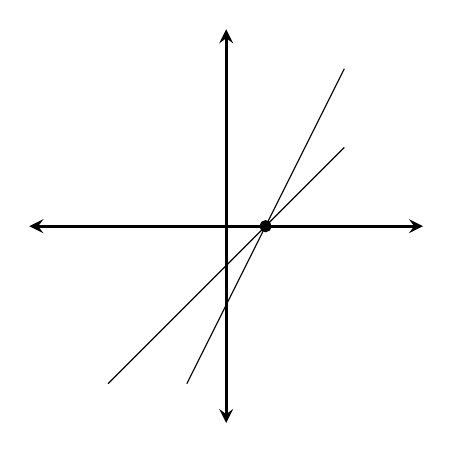
\begin{tikzpicture}
        \draw[black,stealth-stealth,very thick] (0,0) -- (5,0);
        \draw[black,stealth-stealth,very thick] (2.5,-2.5) -- (2.5,2.5);
        \draw (1,-2) -- (4,1);
        \draw (2,-2) -- (4,2);
        \filldraw (3,0) circle (2pt);
        %\node at (0,7) {~};
    \end{tikzpicture}
    {\normalsize\TituloBox{i)} Sistemas con única solución}
\end{flushleft}
~\vspace{-1cm}
\begin{flushleft}
    \begin{tikzpicture}
        \draw[black,stealth-stealth,very thick] (0,0) -- (5,0);
        \draw[black,stealth-stealth,very thick] (2.5,-2.5) -- (2.5,2.5);
        \draw[thick] (1,-2) -- (4,2);
        \draw (1,-2) -- (4,2);
    \end{tikzpicture}
    {\normalsize\TituloBox{ii)} Sistemas con infinitas soluciones}
\end{flushleft}
~\vspace{-1cm}
\begin{flushleft}
    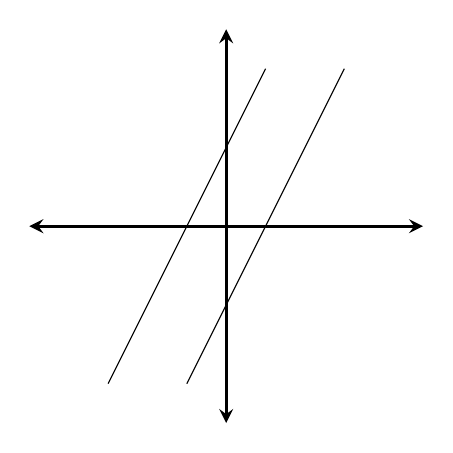
\begin{tikzpicture}
        \draw[black,stealth-stealth,very thick] (12,0) -- (17,0);
        \draw[black,stealth-stealth,very thick] (14.5,-2.5) -- (14.5,2.5);
        \draw (13,-2) -- (15,2);
        \draw (14,-2) -- (16,2);
    \end{tikzpicture}
    {\normalsize\TituloBox{iii)} Sistemas sin solución}
\end{flushleft}
~\vspace{-0.5cm}
\captionsetup*[figure]{font={normalsize},hypcap=false}%
\captionof{figure}{Representación de los posibles casos del conjunto solución de un SEL $2 \times 2$}\label{JWISIKSJSKISOOKKOOOOIUKKSK}
}

Consideremos inicialmente un sistema de dos ecuaciones lineales con dos incógnitas $x_1$ y $x_2$:
\begin{align*}
    a_{11}x_1 + a_{12}x_2 & = b_1 \\ 
    a_{21}x_1 + a_{22}x_2 & = b_2
\end{align*}
donde $a_{11}$, $a_{12}$, $a_{21}$, $a_{22}$, $b_1$, y $b_2$ son coeficientes reales. Geométricamente, cada ecuación representa una recta en el plano cartesiano, y la solución del sistema corresponde a sus puntos de intersección. Este sistema admite tres escenarios posibles: solución única (rectas que se cortan en un punto), infinitas soluciones (rectas coincidentes), o ninguna solución (rectas paralelas no coincidentes), como ilustra la figura \ref{JWISIKSJSKISOOKKOOOOIUKKSK}.

Al extender este concepto al espacio tridimensional, obtenemos un sistema de tres ecuaciones con tres incógnitas $x_1$, $x_2$, y $x_3$:
\begin{align*}
    a_{11}x_1 + a_{12}x_2 + a_{13}x_3 & = b_1 \\ 
    a_{21}x_1 + a_{22}x_2 + a_{23}x_3 & = b_2 \\ 
    a_{31}x_1 + a_{32}x_2 + a_{33}x_3 & = b_3
\end{align*}
donde los coeficientes $a_{ij}$ y términos independientes $b_k$ son números reales. En este caso, cada ecuación describe un plano en el espacio tridimensional, y la solución representa la intersección de estos planos. Análogamente al caso bidimensional, el sistema puede tener: solución única (tres planos que se intersectan en un punto), infinitas soluciones (planos coincidentes o que se cortan formando una recta), o ninguna solución (planos paralelos o sin intersección común). Aunque la visualización geométrica tridimensional es más compleja, la figura \ref{KSKJSJSJJJJSJSJJSDDDD} muestra una representación simplificada de estos posibles casos.
\newpage
\begin{figure*}[h!]
    \centering
    \subfloat[Tres planos se intersecan en un solo punto]{
    \includegraphics[height=0.4\textwidth]{Images/Capitulo2/Plano111.pdf}
    }\hfill
    \subfloat[Tres planos se intersecan en la misma recta]{
    \includegraphics[height=0.4\textwidth]{Images/Capitulo2/Plano222.pdf}
    }\hfill
    \subfloat[Dos planos se intersecan en una recta]{
    \includegraphics[height=0.4\textwidth]{Images/Capitulo2/Plano333.pdf}
    } \hfill
    \subfloat[Los planos paralelos no tienen puntos en común]{
    \includegraphics[height=0.4\textwidth]{Images/Capitulo2/Plano444.pdf}
    }
    \caption{Representación de los posibles casos del conjunto solución de un SEL $3 \times 3$}\label{KSKJSJSJJJJSJSJJSDDDD}
\end{figure*}

La figura \ref{KSKJSJSJJJJSJSJJSDDDD} ilustra cómo interactúan los planos en un sistema de tres ecuaciones lineales con tres incógnitas. Cada caso refleja una relación distinta entre las ecuaciones, lo que determina si el sistema tiene una solución única, infinitas soluciones o ninguna.

Por último, este análisis geométrico sirve como base para introducir nociones más abstractas, como el núcleo y la imagen de una matriz, que exploraremos en la siguiente sección. Estas ideas no solo son esenciales para resolver sistemas, sino también para comprender mejor las estructuras que los sustentan.

\section{Núcleo e imagen de una matriz}

\begin{definicion}{}{}
    Sea $A \in \matrizmn$, se define el \emph{espacio nulo} de $A$, denotado por $\mathcalm{N}(A)$, como:
    $$\mathcalm{N}(A) = \left\{ \mathbb{x} \in \RR[n] \mid A\mathbb{x} = \mathbb{0} \in \RR[m] \right\}$$
    Al espacio nulo de $A$ también de le llama \emph{kernel} de $A$, o bien, \emph{núcleo} de $A$.
\end{definicion}

\begin{theorem}{}{}
    Sea $A \in \matrizmn$, entonces $\mathcalm{N}(A)$ es un subespacio de $\RR[n]$.

    \tcblower
    \demostracion
    \begin{enumerate}[label=\roman*), topsep=6pt, itemsep=0pt]
        \item Sean $\mathbb{x}$, $\mathbb{y} \in \mathcalm{N}(A)$, entonces
        \begin{equation*}
            A\mathbb{x} = \mathbb{0} \quad \text{ y } \quad A\mathbb{y} = \mathbb{0} \label{ec30}
        \end{equation*}
        Ahora
        \begin{align*}
            A(\mathbb{x} + \mathbb{y}) & = A \mathbb{x} + A \mathbb{y} \\
            & = \mathbb{0} + \mathbb{0} \\
            & = \mathbb{0}
        \end{align*}
        Entonces $\mathbb{x} + \mathbb{y} \in \mathcalm{N}(A)$. Por tanto, se cumple la propiedad de cerradura para la suma.
        \item Se deja como ejercicio al lector.
    \end{enumerate}
    De (i) y (ii), se sigue que $\mathcalm{N}(A)$ es subespacio de $\RR[n]$.
\end{theorem}

\begin{definicion}{}{}
    Llamaremos \emph{nulidad} de $A$, denotada por $\nu(A)$, a la dimensión del espacio nulo, es decir,
    $$\nu(A) = \Dim\big(\mathcalm{N}(A)\big).$$
\end{definicion}

\newpage

\begin{examplebox}{}{}
    Determine $\mathcalm{N}(A)$ y $\nu(A)$ de la siguiente matriz
    $$A = \begin{bmatrix*}[r]
        1 & 2 & -1 \\
        2 & -1 & 3
    \end{bmatrix*}$$

    \tcblower
    \solucion Por definición,
    \begin{matrizn}
        \makecell{\includegraphics[page=31]{Externalizacion/C2/MatricesC2.pdf}}
    \end{matrizn}
    Entonces
    \begin{align*}
        x_1 + 2x_2 - x_3 & = 0\\
        2x_1 - x_2 + 3x_3 & = 0
    \end{align*}
    Multiplicando la segunda ecuación por $2$, obtenemos
    \begin{align*}
        x_1 + 2x_2 - x_3 & = 0\\
        4x_1 - 2x_2 + 6x_3 & = 0
    \end{align*}
    Sumando la primer ecuación con la segunda, obtenemos
    $$5x_1 + 5x_3 = 0$$
    Por tanto, $x_3 = -x_1$. Sustituyendo en la primer ecuación, obtenemos
    $$2x_1 + 2x_2 = 0$$
    Por tanto, $x_2 = -x_1$. Se sigue entonces
    \begin{matrizn}
        \makecell{\includegraphics[page=32]{Externalizacion/C2/MatricesC2.pdf}}
    \end{matrizn}
    Por tanto, $\mathcalm{N}(A) = \Gen \left( \left\{ \begin{pNiceMatrix}[cell-space-limits=3pt,r]
        \vphantom{^A}1 \\
        -1 \\
        -1\vphantom{_A}
    \end{pNiceMatrix} \right\} \right)$. Además, $\nu(A) = 1$.
\end{examplebox}

Si $A$ es la matriz cero de tamaño $m \times n$, entonces el sistema se convierte en
$$\mathbb{0}_{m \times n} \mathbb{x} = \mathbb{0}_{n \times 1}.$$
Dado que la matriz cero anula cualquier vector $\mathbb{x} \in \RR[n]$, el sistema siempre tiene todas las soluciones posibles en $\RR[n]$. Esto significa que el espacio nulo de $\mathbb{0}_{m \times n}$ es todo el espacio $\RR[n]$
$$\mathcalm{N}(\mathbb{0}) = \RR[n] \quad \text{ y } \quad \nu(\mathbb{0}) = n.$$
\newpage
%Dado que $\mathcalm{N}(\mathbb{0}) = \RR[n]$, su dimensión es $n$. Es decir,
%$$\nu(\mathbb{0}) = n.$$

\begin{examplebox}{}{}
    Determine $\mathcalm{N}(A)$ y $\nu(A)$ de la siguiente matriz
    $$A = \begin{bmatrix*}[r]
        1 & 2 \\
        1 & -1
    \end{bmatrix*}$$

    \tcblower
    \solucion Por definición,
    \begin{align*}
        \mathcalm{N}(A) & = \left\{ \mathbb{x} \in \RR[2] \mid A\mathbb{x} = \mathbb{0} \in \RR[2] \right\} \\
        & = \left\{ \begin{pmatrix}
            x_1 \\
            x_2
        \end{pmatrix} \in \RR[2] \mid \begin{bmatrix*}[r]
            1 & 2 \\
            1 & -1
        \end{bmatrix*} \begin{bmatrix}
            x_1 \\
            x_2
        \end{bmatrix} = \begin{bmatrix}
            0 \\
            0
        \end{bmatrix} \right\} \\
        & = \left\{ \begin{pmatrix}
            x_1 \\
            x_2
        \end{pmatrix} \in \RR[2] \mid \begin{bmatrix}
            x_1 + 2x_2 \\
            x_1 - x_2
        \end{bmatrix} = \begin{bmatrix}
            0 \\
            0
        \end{bmatrix} \right\}
    \end{align*}
    Entonces
    \begin{align*}
        x_1 + 2x_2 = 0\\
        x_1 - x_2 = 0
    \end{align*}
    Restando la primer ecuación de la segunda, obtenemos que
    $$3x_2 = 0 \Longrightarrow x_2 = 0$$
    y sustituyendo en la segunda ecuación se obtiene que
    $$x_1 = 0$$
    Se sigue entonces que
    $$x_1 = 0 \quad \text{ y } \quad x_2 = 0$$
    por lo que
    \begin{align*}
        \mathcalm{N}(A) & = \left( \left\{ \begin{pmatrix}
            0 \\
            0
        \end{pmatrix} \right\} \right) \\
        & = \Gen \left( \left\{ \begin{pmatrix}
            0 \\
            0
        \end{pmatrix} \right\} \right)
    \end{align*}
    Por tanto, $\mathcalm{N}(A) = \Gen \left( \left\{ \begin{pmatrix}
        0 \\
        0
    \end{pmatrix} \right\} \right)$. Además, $\nu(A) = 0$.
\end{examplebox}

\begin{definicion}{}{}
    Sea $A \in \matrizmn$, se define la \emph{imagen} de $A$, denotado por $\mathcalm{R}(A)$, como
    $$\mathcalm{R}(A) = \left\{ \mathbb{y} \in \RR[m] \mid A\mathbb{x} = \mathbb{y}, \text{ para algún } \mathbb{x} \in \RR[n] \right\}$$
\end{definicion}

\begin{theorem}{}{}
    Sea $A \in \matrizmn$, entonces $\mathcalm{R}(A)$ es un subespacio de $\RR[m]$

    \tcblower
    \demostracion
    \begin{enumerate}[label=\roman*), topsep=6pt, itemsep=0pt]
        \item Sean $\mathbb{y}_1$, $\mathbb{y}_2 \in \mathcalm{R}(A)$, entonces
        \begin{equation}
            A\mathbb{x}_1 = \mathbb{y}_1, \text{ para algún } \mathbb{x}_1 \in \RR[n] \label{UYHDFHDFVFDVFVHFD}
        \end{equation}
        y
        \begin{equation}
            A\mathbb{x}_2 = \mathbb{y}_2, \text{ para algún } \mathbb{x}_2 \in \RR[n] \label{HFHDVJHFHJUGHHFGJ}
        \end{equation}
        Así, de las expresiones \eqref{UYHDFHDFVFDVFVHFD} y \eqref{HFHDVJHFHJUGHHFGJ},
        \begin{align*}
            \mathbb{y}_1 + \mathbb{y}_2 & = A\mathbb{x}_1 + A\mathbb{x}_2 \\
            & = A(\mathbb{x}_1 + \mathbb{x}_2) \\
            & = A\mathbb{w}
        \end{align*}
        siendo $\mathbb{w} = \mathbb{x}_1 + \mathbb{x}_2$. Por tanto, $\mathbb{y}_1 + \mathbb{y}_2 \in \mathcalm{R}(A)$, es decir, se cumple la cerradura bajo la suma.
        \item Se deja como ejercicio al lector.
    \end{enumerate}
    De (i) y (ii), se sigue que $\mathcalm{R}(A)$ es un subespacio de $\RR[m]$.
\end{theorem}

\begin{definicion}{}{}
    Llamaremos \emph{rango} de $A$, denotado por $\rho(A)$, a la dimensión de la imagen, es decir,
    $$\rho(A) = \Dim\big(\mathcalm{R}(A)\big)$$
\end{definicion}

\begin{examplebox}{}{}
    Determine $\mathcalm{R}(A)$ y $\rho(A)$ de la siguiente matriz
    $$A = \begin{bmatrix*}[r]
        1 & 2 \\
        1 & -1
    \end{bmatrix*}$$

    \tcblower
    \solucion Por definición,
    \begin{align*}
        \mathcalm{R}(A) & = \left\{ \mathbb{y} \in \RR[2] \mid A\mathbb{x} = \mathbb{y}, \text{ para algún } \mathbb{x} \in \RR[2] \right\} \\
        & = \left\{ \begin{pmatrix}
            y_1 \\
            y_2
        \end{pmatrix} \in \RR[2] \mid \begin{bmatrix*}[r]
            1 & 2 \\
            1 & -1
        \end{bmatrix*} \begin{bmatrix}
            x_1 \\
            x_2
        \end{bmatrix} = \begin{bmatrix}
            y_1 \\
            y_2
        \end{bmatrix}, \text{ para algún } \mathbb{x} \in \RR[2] \right\} \\
        & = \left\{ \begin{pmatrix}
            y_1 \\
            y_2
        \end{pmatrix} \in \RR[2] \mid \begin{bmatrix}
            x_1 + 2x_2 \\
            x_1 - x_2
        \end{bmatrix} = \begin{bmatrix}
            y_1 \\
            y_2
        \end{bmatrix}, \text{ para algún } \mathbb{x} \in \RR[2] \right\} \\
        & = \left\{ \begin{pmatrix}
            y_1 \\
            y_2
        \end{pmatrix} = x_1 \begin{pmatrix}
            1 \\
            1
        \end{pmatrix} + x_2 \begin{pmatrix*}[r]
            2 \\
            -1
        \end{pmatrix*} \mid x_1, x_2 \in \RR \right\} \\
        & = \Gen \left(\left\{ \begin{pmatrix}
            1 \\
            1
        \end{pmatrix}, \begin{pmatrix*}[r]
            2 \\
            -1
        \end{pmatrix*} \right\}\right)
    \end{align*}
    Observemos que el conjunto de vectores anterior es linealmente independiente. Por tanto, $\mathcalm{R}(A) = \Gen \left(\left\{ \begin{pmatrix}
        1 \\
        1
    \end{pmatrix}, \begin{pmatrix*}[r]
        2 \\
        -1
    \end{pmatrix*} \right\}\right)$ y $\rho(A) = 2$.
\end{examplebox}

\begin{examplebox}{}{matrizrangoe}
    Determine $\mathcalm{R}(A)$ y $\rho(A)$ de la siguiente matriz
    $$A = \begin{bmatrix*}[r]
        1 & 2 & -1 \\
        2 & -1 & 3
    \end{bmatrix*}$$

    \tcblower
    \solucion Por definición,
    \begin{matrizn}
        \makecell{\includegraphics[page=33]{Externalizacion/C2/MatricesC2.pdf}}
    \end{matrizn}
    Observemos que el conjunto anterior de vectores no es linealmente independiente, pues el primer vector puede expresarse como combinación lineal de los otros dos. En particular, si denotamos los vectores respectivamente como $\mathbb{v}_1$, $\mathbb{v}_2$, $\mathbb{v}_3$, entonces existen escalares $\alpha = 1$ y $\beta = 1$ tales que $\mathbb{v}_1 = \alpha \mathbb{v}_2 + \beta \mathbb{v}_3$. Por tanto, esto implica que $\mathcalm{R}(A) = \Gen \left(\left\{ \begin{pmatrix*}[r]
        2 \\
        -1
    \end{pmatrix*}, \begin{pmatrix*}[r]
        -1 \\
        3
    \end{pmatrix*} \right\}\right)$ y $\rho(A) = 2$.
\end{examplebox}

\newpage

\begin{definicion}{}{}
    Si $A \in \matrizmn$, sean $\{ \mathbb{r}_1, \mathbb{r}_2, \dots, \mathbb{r}_m \}$ los renglones de $A$ y $\{ \mathbb{c}_1, \mathbb{c}_2, \dots, \mathbb{c}_n \}$ las columnas de $A$. Es decir,
    \begin{matrizn}
        \makecell{\includegraphics[page=34]{Externalizacion/C2/MatricesC2.pdf}}
    \end{matrizn}
    Definimos el espacio renglón de $A$, denotado por $R_A$, como
    $$R_A = \Gen (\{ \mathbb{r}_1, \mathbb{r}_2, \dots, \mathbb{r}_m \}) \subseteq \RR[n]$$
    y el espacio columna, denotado por $C_A$, como
    $$C_A = \Gen (\{ \mathbb{c}_1, \mathbb{c}_2, \dots, \mathbb{c}_n \}) \subseteq \RR[m]$$
\end{definicion}

\begin{theorem}{}{}
    La imagen de una matriz es igual al espacio columna.

    \tcblower
    \demostracion Para demostrar que $C_A = \mathcalm{R}(A)$, tenemos que demostrar que $\mathcalm{R}(A) \subseteq C_A$ e $C_A \subseteq \mathcalm{R}(A)$.
    \begin{enumerate}[label=\roman*), topsep=6pt, itemsep=0pt]
        \item Queremos probar que $\mathcalm{R}(A) \subseteq C_A$. Supongamos que $\mathbb{y} \in \mathcalm{R}(A)$. Entonces existe un vector $\mathbb{x}$ tal que $\mathbb{y} = A\mathbb{x}$, pero podemos expresa a $A\mathbb{x}$ como una combinación lineal de las columnas de $A$. Para ver esto, consideremos
        \begin{matrizn}
            \makecell{\includegraphics[page=35]{Externalizacion/C2/MatricesC2.pdf}}
        \end{matrizn}
        Entonces
        \begin{matrizn}
            \makecell{\includegraphics[page=36]{Externalizacion/C2/MatricesC2.pdf}}
        \end{matrizn}
        y por consiguiente,
        \begin{matrizn}
            \makecell{\includegraphics[page=37]{Externalizacion/C2/MatricesC2.pdf}}
        \end{matrizn}
        Por lo tanto, $\mathbb{y} \in C_A$, de manera que $\mathcalm{R}(A) \subseteq C_A$.
        \item Se deja como ejercicio al lector.
    \end{enumerate}
\end{theorem}

Si $A$ es la matriz cero de tamaño $m \times n$, entonces el sistema se convierte en
$$\mathbb{0}_{m \times n} \mathbb{x} = \mathbb{y}.$$
Es decir, la única salida posible es el vector cero en $\RR[m]$. Esto implica que
$$\mathcalm{R}(\mathbb{0}) = \{\mathbb{0}_m\}.$$
Esto significa que la imagen de la matriz cero es el subespacio trivial $\{\mathbb{0}_m\}$ en $\RR[m]$. Dado que $\mathcalm{R}(\mathbb{0}) = \{\mathbb{0}_m\}$, su dimensión es 0. Es decir,
$$\rho(\mathbb{0}) = 0.$$

\newpage

\begin{theorem}{}{}
    Si $A$ es una matriz de $m \times n$, entonces
    $$\dim R_A = \dim C_A = \dim\big(\mathcalm{R}(A)\big) = \rho(A)$$

    \tcblower
    \demostracion Denotaremos por $\alpha_{ij}$ la componente $ij$ de $A$. Debemos demostrar que $\dim R_A = \dim C_A$. Los renglones de $A$ se denotan por $\mathbb{r}_1, \mathbb{r}_2, \dots, \mathbb{r}_m$ y sea $k = \dim R_A$. Sea $S = \{\mathbb{s}_1, \mathbb{s}_2, \dots, \mathbb{s}_k\}$ una base para $R_A$. Entonces cada renglón de $A$ se puede expresar como una combinación lineal de los vectores en $S$, y se tiene, para algunas constantes $\alpha_{ij}$,
    \begin{equation}
        \begin{aligned}
            \mathbb{r}_1 & = \alpha_{11} \mathbb{s}_1 + \alpha_{12} \mathbb{s}_2 + \cdots + \alpha_{1k} \mathbb{s}_k \\
            \mathbb{r}_2 & = \alpha_{21} \mathbb{s}_1 + \alpha_{22} \mathbb{s}_2 + \cdots + \alpha_{2k} \mathbb{s}_k \\
            \vdots \\
            \mathbb{r}_m & = \alpha_{m1} \mathbb{s}_1 + \alpha_{m2} \mathbb{s}_2 + \cdots + \alpha_{mk} \mathbb{s}_k
        \end{aligned} \label{ec:rengA5}
    \end{equation}
    Ahora la componente $j$ de $\mathbb{r}_i$ es $a_{ij}$. Entonces si se igualan las componentes $j$ de ambos lados de \eqref{ec:rengA5}, se obtiene
    $$\makecell{\includegraphics[page=38]{Externalizacion/C2/MatricesC2.pdf}}$$
    Es decir,
    \begin{matriz}
        \makecell{\includegraphics[page=39]{Externalizacion/C2/MatricesC2.pdf}} \label{ec:rengA6}
    \end{matriz}
    Entonces como el lado izquierdo de \eqref{ec:rengA6} es la columna $j$ de $A$, se observa que cada columna de $A$ se puede escribir como una combinación lineal de $\mathbb{u}_1, \mathbb{u}_2, \dots, \mathbb{u}_k$, lo que significa que los vectores $\mathbb{u}_1, \mathbb{u}_2, \dots, \mathbb{u}_k$ generan a $C_A$ y
    \begin{equation}
        \dim C_A \leq k = \dim R_A. \label{ec:rengA7}
    \end{equation}
    Pero la ecuación \eqref{ec:rengA7} se cumple para cualquier matriz $A$, y en particular para $A^T$. Pero $C_{A^T} = R_A$ y $R_{A^T} = C_A$. Como de \eqref{ec:rengA7} $\dim C_{A^T} \leq \dim R_{A^T}$, se tiene
    \begin{equation}
        \dim R_A \leq \dim C_A. \label{ec:rengA8}
    \end{equation}
    Combinando \eqref{ec:rengA7} y \eqref{ec:rengA8} la demostración queda completa.
\end{theorem}

\begin{examplebox}{}{}
    Tomando la matriz del ejemplo \ref{examplebox:matrizrangoe}, tenemos que
    $$\makecell{\includegraphics[page=40]{Externalizacion/C2/MatricesC2.pdf}}$$
    De acuerdo con el teorema demostrado previamente, tenemos que
    $$\dim R_A = \dim C_A = \dim\big(\mathcalm{R}(A)\big) = \rho(A)$$
    En este caso particular, se verifica que $\dim R_A = \dim C_A = \dim\big(\mathcalm{R}(A)\big) = 2$.
\end{examplebox}

El siguiente teorema establece una relación fundamental entre el rango y la nulidad de una matriz.

\newpage

\begin{theorem}{}{}
    Si $A$ es una matriz con $n$ columnas, entonces
    \begin{equation}
        \rho(A) + \nu(A) = n. \label{ec:rplusn}
    \end{equation}
\end{theorem}

De lo visto anteriormente, hay seis espacios vectoriales importantes asociados con una matriz $A$ y $A^T$:
$$\begin{array}{ll}
    \text{espacio renglón de } A & \qquad\text{espacio renglón de } A^T \\
    \text{espacio columna de } A & \qquad\text{espacio columna de } A^T \\
    \text{espacio nulo de } A & \qquad\text{espacio nulo de } A^T
\end{array}$$
Sin embargo, transponer una matriz convierte los vectores renglón en vectores columna y viceversa,  
por lo tanto, salvo por una diferencia de notación, el espacio renglón de $A^T$ es el mismo que el espacio columna de $A$, y el espacio columna de $A^T$ es el mismo que el espacio renglón de $A$. Así, de los seis espacios mencionados anteriormente, solo los siguientes cuatro son distintos:
$$\begin{array}{ll}
    \text{espacio renglón de } A & \qquad\text{espacio columna de } A \\
    \text{espacio nulo de } A & \qquad\text{espacio nulo de } A^T
\end{array}$$
A estos se les llama los \textit{espacios fundamentales} de una matriz $A$. Ahora consideraremos cómo se relacionan estos cuatro subespacios.

Pongamos atención por un momento en la matriz $A^T$. Como el espacio renglón y el espacio columna de una matriz tienen la misma dimensión, y como al transponer una matriz se intercambian sus columnas por filas y sus filas por columnas, el siguiente resultado no debería ser sorprendente.
\begin{theorem}{}{rangoaat}
    Si $A$ es cualquier matriz, entonces
    $$\rho(A) = \rho\left(A^T\right).$$

    \tcblower
    \demostracion Es evidente, pues $\rho(A) = \dim(R_A) = \dim(C_{A^T}) = \rho\left(A^T\right)$.
\end{theorem}

Este resultado tiene algunas implicaciones importantes. Por ejemplo, si $A$ es una matriz $m \times n$, entonces al aplicar la fórmula \eqref{ec:rplusn} a la matriz $A^T$ y usando el hecho de que esta matriz tiene $m$ columnas, se obtiene
$$\rho\left(A^T\right) + \nu\left(A^T\right) = m$$
lo cual, en virtud del teorema \ref{theorem:rangoaat}, se puede reescribir como
$$\rho(A) + \nu\left(A^T\right) = m.$$
Esta forma alternativa de la fórmula \eqref{ec:rplusn} permite expresar las dimensiones de los cuatro espacios fundamentales en términos del tamaño y el rango de $A$. Específicamente, si $\rho(A) = r$, entonces
\begin{equation}
    \begin{aligned}
        \dim(R_A) & = r & \dim(C_A) & = r \\
        \dim\big(\mathcalm{N}(A)\big) & = n - r & \qquad\dim\left(\mathcalm{N}\left(A^T\right)\right) & = m - r
    \end{aligned} \label{ec:formulasdimensiones}
\end{equation}
Las cuatro fórmulas en \eqref{ec:formulasdimensiones} proporcionan una relación \textit{algebraica} entre el tamaño de una matriz y las dimensiones de sus espacios fundamentales.

\begin{examplebox}{}{}
    ¿Cuál es el rango máximo posible de una matriz $m \times n$ que no es cuadrada?

    \tcblower
    \solucion Dado que los vectores renglón de $A$ pertenecen a $\RR[n]$ y los vectores columna a $\RR[m]$, el espacio renglón de $A$ tiene como máximo dimensión $n$ y el espacio columna como máximo dimensión $m$. Como el rango de $A$ es la dimensión común de su espacio renglón y su espacio columna, se deduce que el rango es como máximo el menor entre $m$ y $n$. Esto se expresa como: $\rho(A) \leq \min(m, n)$.
\end{examplebox}

\newpage

\section{Operaciones elementales en los renglones de una matriz}

Las operaciones elementales por renglón son un conjunto de tres operaciones básicas que se pueden aplicar a los renglones de una matriz sin alterar el espacio renglón de la misma. Estas operaciones son fundamentales en el álgebra lineal para simplificar matrices y resolver sistemas de ecuaciones lineales. La idea principal es manipular la matriz de manera sistemática para alcanzar una forma más sencilla, como la forma escalonada o la forma escalonada reducida, lo que facilita el análisis de sus propiedades. Así, dada una matriz, las operaciones elementales son:
\begin{itemize}
    \item \textbf{Intercambiar dos renglones:} Si intercambiamos los renglones $i$ y $j$, escribiremos $\mathbb{r}_i \rightleftarrows \mathbb{r}_j$.
    \item \textbf{Multiplicar un renglón por una constante no cero:} Si multiplicamos el renglón $i$ por la constante no cero $\alpha$, escribiremos $\mathbb{r}_i \leftarrow \alpha\mathbb{r}_i$.
    \item \textbf{Sumarle a un renglón un múltiplo de otro renglón:} Si le sumamos al renglón $i$, $\alpha$-veces el renglón $j$, escribiremos $\mathbb{r}_i \leftarrow \mathbb{r}_i + \alpha\mathbb{r}_j$.
\end{itemize}
Para denotar una operación elemental, se utiliza una flecha orientada hacia la derecha que indica el paso de una matriz a otra. Encima de esta flecha se escribe la operación elemental correspondiente, especificando claramente qué tipo de operación se está realizando. Por ejemplo:
$$\begin{bmatrix}
    1 & 2 \\
    3 & 4
\end{bmatrix} \xrightarrow{\mathbb{r}_1 \rightleftarrows \mathbb{r}_2} \begin{bmatrix}
    3 & 4 \\
    1 & 2
\end{bmatrix}, \quad \begin{bmatrix}
    1 & 2 \\
    3 & 4
\end{bmatrix} \xrightarrow{\mathbb{r}_1 \leftarrow 3\mathbb{r}_1} \begin{bmatrix}
    3 & 6 \\
    3 & 4
\end{bmatrix}, \quad \begin{bmatrix}
    1 & 2 \\
    3 & 4
\end{bmatrix} \xrightarrow{\mathbb{r}_2 \leftarrow \mathbb{r}_2 + 2\mathbb{r}_1} \begin{bmatrix}
    1 & 2 \\
    5 & 8
\end{bmatrix}$$

\begin{definicion}{}{}
    Sean $A$, $B \in \matrizmn$. Decimos que $A$ es equivalente por renglones a $B$, si existe un número finito de operaciones elementales tales que al aplicárselas a la matriz $A$ se obtiene la matriz $B$.
\end{definicion}

\begin{definicion}{}{}
    Decimos que una matriz $A \in \matrizmn$ está en forma escalonada si:
    \begin{enumerate}[label=\roman*), topsep=6pt, itemsep=0pt]
        \item Los renglones cero están en la parte inferior de la matriz.
        \item Los renglones no cero satisfacen que su primera entrada no cero es 1, llamado uno principal.
        \item En dos renglones no cero consecutivos, el uno principal del renglón inferior aparece más a la derecha que el uno principal del renglón superior.
    \end{enumerate}
\end{definicion}

\begin{examplebox}{}{}
    Un ejemplo muy claro es
    \begin{matrizn}
        \makecell{\includegraphics[page=41]{Externalizacion/C2/MatricesC2.pdf}}
    \end{matrizn}
    Esta matriz está en forma escalonada, ya que:
    \begin{enumerate}[label=\roman*), topsep=6pt, itemsep=0pt]
        \item Esta matriz no tiene renglones completamente cero, por lo que la primer condición se cumple trivialmente.
        \item En el primer renglón, la primera entrada no cero es $1$ (columna 1). En el segundo renglón, la primera entrada no cero es $1$ (columna 2, después del cero inicial). En el tercer renglón, la primera entrada no cero es $1$ (columna 4). Todos los renglones no cero cumplen con la segunda condición.
        \item Del primer al segundo renglón, el uno principal del segundo renglón (columna 2) está a la derecha del uno principal del primer renglón (columna 1). Del segundo al tercer renglón, el uno principal del tercer renglón (columna 4) está a la derecha del uno principal del segundo renglón (columna 2). Esto satisface la tercer condición. 
    \end{enumerate}
\end{examplebox}

\newpage

\begin{definicion}{}{}
    Decimos que una matriz $A \in \matrizmn$ está en forma escalonada reducida si la matriz está en forma escalonada y cada columna que contenga un uno principal tiene ceros en todas sus demás entradas.
\end{definicion}

\begin{examplebox}{}{}
    Un ejemplo muy claro es
    \begin{matrizn}
        \makecell{\includegraphics[page=42]{Externalizacion/C2/MatricesC2.pdf}}
    \end{matrizn}
    Esta matriz está en forma escalonada reducida, ya que: está en forma escalonada y cada columna con un uno principal (columnas 1, 2 y 4) tiene ceros en todas las demás entradas. La columna 3 no tiene un uno principal, por lo que no hay restricción.
\end{examplebox}

\begin{theorem}{}{}
    Toda matriz tamaño $m \times n$ no cero es equivalente por renglones a una matriz en forma escalonada.
\end{theorem}

\begin{theorem}{}{}
    Toda matriz tamaño $m \times n$ no cero es equivalente por renglones a una única matriz en forma escalonada reducida.
\end{theorem}

Después de haber definido ya las tres operaciones elementales sobre renglones, estamos en condiciones de usarlas para resolver sistemas de ecuaciones lineales de manera sistemática.

A medida que aumenta el número de ecuaciones e incógnitas en un sistema lineal, también lo hace la complejidad del álgebra involucrado en encontrar soluciones. Los cálculos requeridos pueden hacerse más manejables simplificando la notación y estandarizando los procedimientos. Del sistema visto en \eqref{ec29}, podemos abreviar el sistema escribiendo únicamente el arreglo rectangular de números como
$$\makecell{\includegraphics[page=43]{Externalizacion/C2/MatricesC2.pdf}}$$
Esto se llama la \emph{matriz aumentada} del sistema. Por ejemplo, la matriz aumentada para el sistema de ecuaciones
\begin{matrizn}
    \makecell{\includegraphics[page=44]{Externalizacion/C2/MatricesC2.pdf}}
\end{matrizn}

\begin{adjustwidth}{-7.6cm}{-2cm}
    \begin{tcolorbox}[
        theorem style=change break,
        enhanced,
        breakable,
        boxrule=0pt,
        frame hidden,
        left = 1.8cm,
        right = 1.8cm,
        top=4mm,
        bottom=2mm,
        colback=black!7!white,
        coltitle=black,
        attach title to upper={\ },
        sharp corners,
        borderline north={1.5pt}{0pt}{black},
        title = {Método de eliminación Gaussiana:},
        fonttitle=\selectfont\Lato\bfseries\LARGE,
        fontupper=\normalsize
    ]
        \,\\[4mm]
        La eliminación Gaussiana es un método algebraico utilizado para resolver sistemas de ecuaciones lineales. Consiste en transformar una matriz aumentada del sistema en una forma escalonada mediante operaciones elementales por renglones. El procedimiento es el siguiente:\vspace{0.3cm}
        \begin{enumerate}
            \item Considerar la matriz aumentada del sistema, llamémosle $A$.
            \item Aplicar a la matriz $A$ operaciones elementales hasta obtener una matriz en forma escalonada, llamémosle $R$.
            \item Escribir el sistema de ecuaciones que tiene por matriz aumentada a la matriz $R$.
            \item Se despeja el valor de la última incógnita que esté asociada a un uno principal.
            \item Se usa la sustitución hacia atrás para determinar las demás incógnitas que estén asociadas a un uno principal.
            \item Escribir el conjunto solución, llamémosle $S$.
        \end{enumerate}
    \end{tcolorbox}
\end{adjustwidth}

\newpage

\begin{examplebox}{}{}
    Resuelva el siguiente sistema por el método de eliminación Gaussiana:
    \begin{align*}
        -x - y + 3z & = -1 \\
        5x - y - 3z & = -7 \\
        4x + 3y + z & = 2
    \end{align*}

    \tcblower
    \solucion Apliquemos el método de eliminación Gaussiana. Primero formamos la matriz aumentada del sistema, la cual es
    \begin{matrizn}
        \makecell{\includegraphics[page=45]{Externalizacion/C2/MatricesC2.pdf}}
    \end{matrizn}
    Ahora, aplicamos operaciones elementales hasta llevarla a su forma escalonada. Sumando 5 veces el primer renglón al segundo renglón, obtenemos
    \begin{matrizn}
        \makecell{\includegraphics[page=46]{Externalizacion/C2/MatricesC2.pdf}}
    \end{matrizn}
    Sumando 4 veces el primer renglón al tercer renglón, obtenemos
    \begin{matrizn}
        \makecell{\includegraphics[page=47]{Externalizacion/C2/MatricesC2.pdf}}
    \end{matrizn}
    Multiplicando por $-1$ el primer renglón, obtenemos
    \begin{matrizn}
        \makecell{\includegraphics[page=48]{Externalizacion/C2/MatricesC2.pdf}}
    \end{matrizn}
    Multiplicando por $-\dfrac{1}{6}$ el segundo renglón, obtenemos
    \begin{matrizn}
        \makecell{\includegraphics[page=49]{Externalizacion/C2/MatricesC2.pdf}}
    \end{matrizn}
    Sumando 1 vez el segundo renglón al tercer renglón, obtenemos
    \begin{matrizn}
        \makecell{\includegraphics[page=50]{Externalizacion/C2/MatricesC2.pdf}}
    \end{matrizn}
    Multiplicando por $\dfrac{1}{11}$ el tercer renglón, obtenemos
    \begin{matrizn}
        \makecell{\includegraphics[page=51]{Externalizacion/C2/MatricesC2.pdf}}
    \end{matrizn}
    Ahora bien, escribimos el sistema de ecuaciones que tiene por matriz aumentada a la matriz $R$:
    \begin{align*}
        x + y - 3z & = 1 \\
        y - 2z & = 2 \\
        z & = 0
    \end{align*}
    Del sistema, ya sabemos que $z = 0$, sustituyendo en la segunda ecuación obtenemos que $y = 2$. Luego, sustituyendo estos dos valores en la primer ecuación obtenemos que $x = -1$. Por lo tanto, el conjunto solución es
    \begin{matrizn}
        \makecell{\includegraphics[page=52]{Externalizacion/C2/MatricesC2.pdf}}
    \end{matrizn}
\end{examplebox}

\newpage

Es importante destacar que no existe un único camino para resolver un sistema de ecuaciones lineales. Aunque todos los caminos correctos conducen, en principio, a la misma solución (si existe una), las operaciones que se aplican pueden variar dependiendo de la estrategia o del orden en que se elijan. Esta flexibilidad también implica que es fundamental verificar cuidadosamente cada paso, ya que una mala elección o un error de cálculo puede llevar a una matriz incorrecta.

\begin{adjustwidth}{-7.6cm}{-2cm}
    \begin{tcolorbox}[
        theorem style=change break,
        enhanced,
        breakable,
        boxrule=0pt,
        frame hidden,
        left = 1.8cm,
        right = 1.8cm,
        top=4mm,
        bottom=2mm,
        colback=black!7!white,
        coltitle=black,
        attach title to upper={\ },
        sharp corners,
        borderline north={1.5pt}{0pt}{black},
        title = {Método de eliminación Gauss-Jordan:},
        fonttitle=\selectfont\Lato\bfseries\LARGE,
        fontupper=\normalsize
    ]
        \,\\[4mm]
        La eliminación Gauss-Jordan es también un método algebraico utilizado para resolver sistemas de ecuaciones lineales. Este método es una extensión natural de la eliminación gaussiana, y tiene como objetivo llevar la matriz no sólo a una forma más sencilla, sino a su forma más reducida mediante operaciones elementales por renglones. El procedimiento es el siguiente:\vspace{0.3cm}
        \begin{enumerate}
            \item Considerar la matriz aumentada del sistema, llamémosle $A$.
            \item Aplicar a la matriz $A$ operaciones elementales hasta obtener una matriz en forma escalonada reducida, llamémosle $R$.
            \item Escribir el sistema de ecuaciones que tiene por matriz aumentada a la matriz $R$.
            \item Despejar las incógnitas que estén asociadas a un uno principal.
            \item Escribir el conjunto solución, llamémosle $S$.
        \end{enumerate}
    \end{tcolorbox}
\end{adjustwidth}

\begin{examplebox}{}{}
    Resuelva el siguiente sistema por el método de eliminación Gauss-Jordan:
    \begin{align*}
        x + 3y - 2z & = 1 \\
        2x - 9y + 2z & = 2 \\
        9x + 4y + 2z & = 9
    \end{align*}

    \tcblower
    \solucion Apliquemos el método de eliminación Gauss-Jordan. Primero formamos la matriz aumentada del sistema, la cual es
    \begin{matrizn}
        \makecell{\includegraphics[page=53]{Externalizacion/C2/MatricesC2.pdf}}
    \end{matrizn}
    Ahora, aplicamos operaciones elementales hasta llevarla a su forma escalonada reducida. Sumando $-2$ veces el primer renglón al segundo renglón, obtenemos
    \begin{matrizn}
        \makecell{\includegraphics[page=54]{Externalizacion/C2/MatricesC2.pdf}}
    \end{matrizn}
    Sumando $-9$ veces el primer renglón al tercer renglón, obtenemos
    \begin{matrizn}
        \makecell{\includegraphics[page=55]{Externalizacion/C2/MatricesC2.pdf}}
    \end{matrizn}
    Multiplicando por $\dfrac{1}{3}$ el segundo renglón, obtenemos
    \begin{matrizn}
        \makecell{\includegraphics[page=56]{Externalizacion/C2/MatricesC2.pdf}}
    \end{matrizn}
    Sumando 1 vez el primer renglón al segundo renglón, obtenemos
    \begin{matrizn}
        \makecell{\includegraphics[page=57]{Externalizacion/C2/MatricesC2.pdf}}
    \end{matrizn}
    \newpage
    Sumando $-10$ veces el segundo renglón al tercer renglón, obtenemos
    \begin{matrizn}
        \makecell{\includegraphics[page=58]{Externalizacion/C2/MatricesC2.pdf}}
    \end{matrizn}
    Multiplicando por $\dfrac{1}{27}$ el tercer renglón, obtenemos
    \begin{matrizn}
        \makecell{\includegraphics[page=59]{Externalizacion/C2/MatricesC2.pdf}}
    \end{matrizn}
    Sumando 5 veces el tercer renglón al segundo renglón, obtenemos
    \begin{matrizn}
        \makecell{\includegraphics[page=60]{Externalizacion/C2/MatricesC2.pdf}}
    \end{matrizn}
    Sumando 2 veces el tercer renglón al primer renglón, obtenemos
    \begin{matrizn}
        \makecell{\includegraphics[page=61]{Externalizacion/C2/MatricesC2.pdf}}
    \end{matrizn}
    Intercambiando el segundo renglón y el tercer renglón, obtenemos
    \begin{matrizn}
        \makecell{\includegraphics[page=62]{Externalizacion/C2/MatricesC2.pdf}}
    \end{matrizn}
    Multiplicando por $\dfrac{1}{2}$ el tercer renglón, obtenemos
    \begin{matrizn}
        \makecell{\includegraphics[page=63]{Externalizacion/C2/MatricesC2.pdf}}
    \end{matrizn}
    Ahora bien, escribimos el sistema de ecuaciones que tiene por matriz aumentada a la matriz $R$:
    \begin{align*}
        x & = 1 \\
        y & = 0 \\
        z & = 0
    \end{align*}
    Pero las incógnitas ya están despejadas. Por lo tanto, el conjunto solución es
    \begin{matrizn}
        \makecell{\includegraphics[page=64]{Externalizacion/C2/MatricesC2.pdf}}
    \end{matrizn}
\end{examplebox}

\begin{examplebox}{}{}
    Encuentra la nulidad y el rango de la matriz
    $$\makecell{\includegraphics[page=65]{Externalizacion/C2/MatricesC2.pdf}}$$

    \tcblower
    \solucion Para poder encontrar la nulidad de la matriz $A$, primero debemos encontrar el espacio nulo de $A$. Sin embargo, por definición es equivalente a encontrar la solución de $A\mathbb{x} = \mathbb{0}$. También podemos aplicar el método de eliminación de Gauss-Jordan. Formamos la matriz aumentada,
    \begin{matrizn}
        \makecell{\includegraphics[page=66]{Externalizacion/C2/MatricesC2.pdf}}
    \end{matrizn}
    Aplicando operaciones elementales a dicha matriz, obtenemos que su forma escalonada reducida es (verificar):
    \begin{matriz}
        \makecell{\includegraphics[page=67]{Externalizacion/C2/MatricesC2.pdf}} \label{matrixescalonada}
    \end{matriz}
    Por tanto, el sistema correspondiente de ecuaciones es
    \begin{align*}
        x_1 - 4x_3 - 28x_4 - 37x_5 + 13x_6 & = 0 \\
        x_2 - 2x_3 - 12x_4 - 16x_5 + 5x_6 & = 0
    \end{align*}
    Despejando las incógnitas que estén asociadas a un uno principal, tenemos que
    \begin{align*}
       x_1 & = 4x_3 + 28x_4 + 37x_5 - 13x_6 \\
       x_2 & = 2x_3 + 12x_4 + 16x_5 - 5x_6
    \end{align*}
    Resolviendo estas ecuaciones para las variables principales se obtiene
    \begin{align*}
        x_1 & = 4r + 28s + 37t - 13u \\
        x_2 & = 2r + 12s + 16t - 5u \\
        x_3 & = r \\
        x_4 & = s \\
        x_5 & = t \\
        x_6 & = u
    \end{align*}
    Por lo tanto, el conjunto solución del sistema homogéneo es
    \begin{matrizn}
        \makecell{\includegraphics[page=68]{Externalizacion/C2/MatricesC2.pdf}}
    \end{matrizn}
    Es decir,
    $$\makecell{\includegraphics[page=69]{Externalizacion/C2/MatricesC2.pdf}}$$
    de donde se sigue que $\nu(A) = 4$. Para hallar el rango de $A$, debemos encontrar la dimensión del espacio solución del sistema lineal $A\mathbb{x} = \mathbb{y}$. Este sistema puede resolverse reduciendo la matriz aumentada a su forma escalonada reducida. La matriz resultante será idéntica a la de \eqref{matrixescalonada}, excepto que no tendrá una columna adicional de ceros al final, y dado que esta matriz tiene dos unos principales, su espacio columna es bidimensional y $\rho(A) = 2$.
\end{examplebox}

\newpage

\section{Matrices no singulares y matrices elementales}

En los números reales, todo número no nulo $a$ tiene un recíproco $a^{-1}$ con la propiedad
$$a \cdot a^{-1} = a^{-1} \cdot a = 1.$$
Al número $a^{-1}$ se le llama comúnmente como el \emph{inverso multiplicativo} de $a$. Nuestro siguiente objetivo es desarrollar un análogo de este resultado para la aritmética de matrices. Para este propósito, hacemos la siguiente definición.

\begin{definicion}{}{}
    Si $A$ es una matriz cuadrada y si se puede encontrar una matriz $B$ del mismo tamaño tal que $AB = BA = I$, entonces se dice que $A$ es \emph{invertible} o \emph{no singular} y que $B$ es una \textit{inversa} de $A$. Si no se puede encontrar tal matriz $B$, entonces se dice que $A$ es \emph{no invertible} o \textit{singular}.
\end{definicion}

La relación $AB = BA = I$ no cambia al intercambiar $A$ y $B$, así que si $A$ es invertible y $B$ es una inversa de $A$, entonces también es cierto que $B$ es invertible y $A$ es una inversa de $B$. Así, cuando
$$AB = BA = I$$
decimos que $A$ y $B$ son \emph{inversas una de la otra}.

\begin{examplebox}{}{}
    Sean
    $$A = \begin{bmatrix*}[r]
        2 & -5 \\
        -1 & 3
    \end{bmatrix*} \quad \text{ y } \quad B = \begin{bmatrix}
        3 & 5 \\
        1 & 2
    \end{bmatrix}.$$
    Entonces
    \begin{align*}
        AB & = \begin{bmatrix*}[r]
            2 & -5 \\
            -1 & 3
        \end{bmatrix*} \begin{bmatrix}
            3 & 5 \\
            1 & 2
        \end{bmatrix} = \begin{bmatrix}
            1 & 0 \\
            0 & 1
        \end{bmatrix} = I \\
        BA & = \begin{bmatrix}
            3 & 5 \\
            1 & 2
        \end{bmatrix} \begin{bmatrix*}[r]
            2 & -5 \\
            -1 & 3
        \end{bmatrix*} = \begin{bmatrix}
            1 & 0 \\
            0 & 1
        \end{bmatrix} = I
    \end{align*}
    Por lo tanto, $A$ y $B$ son no singulares y cada una es inversa de la otra.
\end{examplebox}

Es razonable preguntarse si una matriz invertible puede tener más de una inversa. El siguiente teorema muestra que la respuesta es no: una matriz invertible tiene exactamente una inversa.

\begin{theorem}{}{}
    Si $B$ y $C$ son ambas inversas de la matriz $A$, entonces $B = C$.

    \tcblower
    \demostracion Como $B$ es una inversa de $A$, tenemos que $BA = I$. Multiplicando ambos lados por la derecha con $C$ se obtiene
    $$(BA)C = IC = C.$$
    Pero también es cierto que
    $$(BA)C = B(AC) = BI = B,$$
    por lo tanto, $C = B$.
\end{theorem}

Como consecuencia de este resultado importante, ahora podemos hablar de “la” inversa de una matriz invertible. Si $A$ es invertible, entonces su inversa se denotará con el símbolo $A^{-1}$. Así,\infoBulle{El símbolo $A^{-1}$ no debe interpretarse como $1/A$. La división entre matrices no será una operación definida en este texto.}
$$AA^{-1} = I \quad \text{ y } \quad A^{-1}A = I.$$
La inversa de $A$ cumple un papel muy similar en la aritmética de matrices al que cumple el recíproco $a^{-1}$ en las relaciones numéricas $aa^{-1} = 1$ y $a^{-1}a = 1$.

\newpage

El siguiente teorema se refiere a las inversas de productos de matrices.

\begin{theorem}{}{}
    Si $A$ y $B$ son matrices invertibles del mismo tamaño, entonces $AB$ es invertible y
    $$(AB)^{-1} = B^{-1}A^{-1}.$$

    \tcblower
    \demostracion Podemos establecer que $AB$ es invertible y obtener la fórmula dada al mismo tiempo, mostrando que
    $$(AB)\left(B^{-1}A^{-1}\right) = \left(B^{-1}A^{-1}\right)(AB) = I.$$
    Pero
    $$(AB)\left(B^{-1}A^{-1}\right) = A\left(BB^{-1}\right)A^{-1} = AIA^{-1} = AA^{-1} = I$$
    y de manera similar,
    $$\left(B^{-1}A^{-1}\right)(AB) = I.$$
\end{theorem}

Aunque no lo demostraremos, este resultado puede extenderse a tres o más factores: El producto de cualquier cantidad de matrices invertibles es invertible, y la inversa del producto es el producto de las inversas en orden inverso.

\begin{examplebox}{}{}
    Consideremos las matrices
    $$A = \begin{bmatrix} 1 & 2 \\ 3 & 5 \end{bmatrix}, \quad B = \begin{bmatrix} 2 & 3 \\ 1 & 2 \end{bmatrix}.$$
    Tenemos que
    $$AB = \begin{bmatrix} 4 & 7 \\ 11 & 19 \end{bmatrix}, \quad (AB)^{-1} = \begin{bmatrix*}[r] -19 & 7 \\ 11 & -4 \end{bmatrix*}$$
    y también que
    $$A^{-1} = \begin{bmatrix*}[r] -5 & 2 \\ 3 & -1 \end{bmatrix*}, \quad B^{-1} = \begin{bmatrix*}[r] 2 & -3 \\ -1 & 2 \end{bmatrix*}, \quad B^{-1}A^{-1} = \begin{bmatrix*}[r] -19 & 7 \\ 11 & -4 \end{bmatrix*}.$$
    Así, $(AB)^{-1} = B^{-1}A^{-1}$ como lo garantiza el teorema anterior.
\end{examplebox}

Si $A$ es una matriz cuadrada invertible, entonces definimos las potencias enteras negativas de $A$ como
$$A^{-n} = \left(A^{-1}\right)^n = \underbrace{A^{-1}A^{-1} \cdots A^{-1}}_{n-\text{veces}}$$
Dado que estas definiciones son análogas a las de los números reales, se cumplen las leyes usuales de exponentes no negativos. Por ejemplo,
$$A^r A^s = A^{r+s} \quad \text{ y } \quad \left(A^r\right)^s = A^{rs}.$$
Además, tenemos las siguientes propiedades para exponentes negativos:
\begin{theorem}{}{propiedadesninv}
    Si $A$ es invertible y $n$ es un entero no negativo, entonces:
    \begin{enumerate}[label=\alph*), topsep=6pt, itemsep=0pt]
        \item $A^{-1}$ es invertible y $\left(A^{-1}\right)^{-1} = A$.
        \item $A^n$ es invertible y $\left(A^n\right)^{-1} = A^{-n} = \left(A^{-1}\right)^n$.
        \item $kA$ es invertible para todo escalar $k \neq 0$, y $(kA)^{-1} = k^{-1} A^{-1}$.
    \end{enumerate}
\end{theorem}

El siguiente teorema establece una relación entre la inversa de una matriz y la inversa de su transpuesta.

\begin{theorem}{}{}
    Si $A$ es una matriz invertible, entonces $A^T$ también es invertible y
    $$\left(A^T\right)^{-1} = \left(A^{-1}\right)^T.$$
\end{theorem}

\newpage

\begin{examplebox}{}{}
    Consideremos las matrices
    $$A = \begin{bmatrix*}[r] 1 & 2 \\ 1 & 3 \end{bmatrix*} \quad \text{ y } \quad A^{-1} = \begin{bmatrix*}[r] 3 & -2 \\ -1 & 1 \end{bmatrix*}.$$
    Entonces,
    $$A^{-3} = \left(A^{-1}\right)^3 = \begin{bmatrix*}[r] 3 & -2 \\ -1 & 1 \end{bmatrix*} \begin{bmatrix*}[r] 3 & -2 \\ -1 & 1 \end{bmatrix*} \begin{bmatrix*}[r] 3 & -2 \\ -1 & 1 \end{bmatrix*} = \begin{bmatrix*}[r] 41 & -30 \\ -15 & 11 \end{bmatrix*}.$$
    También,
    $$A^3 = \begin{bmatrix*}[r] 1 & 2 \\ 1 & 3 \end{bmatrix*} \begin{bmatrix*}[r] 1 & 2 \\ 1 & 3 \end{bmatrix*} \begin{bmatrix*}[r] 1 & 2 \\ 1 & 3 \end{bmatrix*} = \begin{bmatrix} 11 & 30 \\ 15 & 41 \end{bmatrix}.$$
    Por lo tanto, como se esperaba según el teorema \ref{theorem:propiedadesninv}b),
    $$\left(A^3\right)^{-1} = \begin{bmatrix*}[r] 41 & -30 \\ -15 & 11 \end{bmatrix*} = \left(A^{-1}\right)^3.$$
\end{examplebox}

\begin{examplebox}{}{}
    En la aritmética real, donde existe una ley conmutativa para la multiplicación, podemos escribir
    $$(a + b)^2 = a^2 + ab + ba + b^2 = a^2 + ab + ab + b^2 = a^2 + 2ab + b^2.$$
    Sin embargo, en la aritmética de matrices, donde no existe una ley conmutativa para la multiplicación, lo mejor que podemos hacer es escribir
    $$(A + B)^2 = A^2 + AB + BA + B^2.$$
    Solo en el caso especial en que $A$ y $B$ conmutan (es decir, $AB = BA$) podemos ir un paso más allá y escribir
    $$(A + B)^2 = A^2 + 2AB + B^2.$$
\end{examplebox}

\begin{examplebox}{}{}
    Una matriz cuadrada con un renglón o una columna de ceros es singular. Para ayudar a entender por qué, consideremos la matriz
    $$\makecell{\includegraphics[page=70]{Externalizacion/C2/MatricesC2.pdf}}$$
    Para probar que $A$ es singular, debemos mostrar que no existe una matriz $B$ de tamaño $4 \times 4$ tal que $AB = BA = I$. Con este propósito, sean
    $$\makecell{\includegraphics[page=71]{Externalizacion/C2/MatricesC2.pdf}}$$
    las columnas de $A$. Entonces, para cualquier matriz $B$ de tamaño $4 \times 4$, podemos expresar el producto $BA$ como
    $$BA = B \begin{bmatrix}
        \mathbb{c}_1 & \mathbb{c}_2 & \mathbb{c}_3 & \mathbb{0}
    \end{bmatrix} = \begin{bmatrix}
        B\mathbb{c}_1 & B\mathbb{c}_2 & B\mathbb{c}_3 & B\mathbb{0}
    \end{bmatrix}.$$
    La columna de ceros muestra que $BA \neq I$ y, por lo tanto, $A$ es singular.
\end{examplebox}

Nuestro próximo objetivo es mostrar cómo se puede utilizar la multiplicación de matrices para realizar una operación elemental por renglón.

\begin{definicion}{}{}
    Una matriz $E$ se denomina \emph{matriz elemental} si dicha matriz se obtiene de la matriz identidad, aplicando solo una operación elemental.
\end{definicion}

\newpage

\begin{examplebox}{}{}
    Las siguientes tres matrices elementales son obtenidas de $I_3$ aplicando las operaciones elementales en sus renglones vistas en la sección anterior.
    \begin{itemize}[topsep=6pt, itemsep=0pt]
        \item Intercambiando el primer renglón y el tercer renglón, se obtiene
        \begin{matrizn}
            \makecell{\includegraphics[page=72]{Externalizacion/C2/MatricesC2.pdf}}
        \end{matrizn}
        \item Multiplicando por $-3$ el segundo renglón, se obtiene
        \begin{matrizn}
            \makecell{\includegraphics[page=73]{Externalizacion/C2/MatricesC2.pdf}}
        \end{matrizn}
        \item Sumando 3 veces el tercer renglón al primer renglón, se obtiene
        \begin{matrizn}
            \makecell{\includegraphics[page=74]{Externalizacion/C2/MatricesC2.pdf}}
        \end{matrizn}
    \end{itemize}
\end{examplebox}

El siguiente teorema, cuya demostración se deja como ejercicio al lector, muestra que cuando una matriz $A$ se multiplica por la izquierda por una matriz elemental $E$, el efecto es realizar una operación elemental por renglones sobre $A$.

\begin{theorem}{}{prodelem}
    Si la matriz elemental $E$ resulta de realizar una cierta operación elemental sobre $I_m$, y si $A$ es una matriz $m \times n$, entonces el producto $EA$ es la matriz que resulta al realizar esa misma operación elemental sobre $A$.
\end{theorem}

\begin{corollary}{}{}
    Sean $A$ y $B$ matrices de trabajo $m \times n$, entonces $A$ es equivalente por renglones si y solo si existen $E_1, E_2, \dots E_r$ matrices elementales obtenidas de realizar una cierta operación elemental sobre $I_m$, tales que $E_r \cdots E_2E_1A = B$.
\end{corollary}

\begin{examplebox}{}{}
    Consideremos la matriz
    $$\makecell{\includegraphics[page=75]{Externalizacion/C2/MatricesC2.pdf}}$$
    y consideremos la matriz elemental
    $$\makecell{\includegraphics[page=76]{Externalizacion/C2/MatricesC2.pdf}}$$
    que es obtenida de sumar 3 veces el primer renglón de $I_3$ al tercer renglón. El producto $EA$ es
    $$\makecell{\includegraphics[page=77]{Externalizacion/C2/MatricesC2.pdf}}$$
    que es precisamente la matriz que resulta de sumar 3 veces el primer renglón de $A$ al tercer renglón.
\end{examplebox}

Sabemos que si $E$ es una matriz elemental que resulta de realizar una operación elemental sobre la matriz identidad $I$, entonces existe una segunda operación elemental que, al aplicarse a $E$, produce nuevamente la identidad $I$. La tabla \ref{tab:operacionesinversas} enumera estas operaciones. Las operaciones del lado derecho de la tabla se denominan \textit{operaciones inversas} de las correspondientes operaciones del lado izquierdo.

\newpage

Esto implica que toda matriz elemental es invertible, y su inversa también es una matriz elemental. Más aún, al aplicar una operación y su inversa de manera sucesiva, se recupera exactamente el estado original de la matriz.
\begin{table}[h!]
    \centering
    \begin{NiceTabular}{cc}[hvlines,cell-space-limits=5pt]
        \CodeBefore
        \rowcolor{black!20!white}{1}
        \Body
        \makecell{Operación elemental sobre \\ $I$ que produce $E$} & \makecell{Operación elemental sobre \\ $E$ que reproduce $I$} \\
        Intercambiar los renglones $i$ y $j$ & Intercambiar los renglones $i$ y $j$ \\
        \makecell{Multiplicar el $i$-ésimo renglón \\ por una constante $c \neq 0$} & \makecell{Multiplicar el $i$-ésimo renglón \\ por una constante $c^{-1}$} \\
        \makecell{Sumar $c$ veces el renglón \\ $i$ al renglón $j$} & \makecell{Sumar $-c$ veces el renglón \\ $i$ al renglón $j$}
    \end{NiceTabular}
    \caption{Operaciones elementales y sus inversas}
    \label{tab:operacionesinversas}
\end{table}

El siguiente teorema es un resultado clave sobre la invertibilidad de matrices elementales. Servirá como base para muchos resultados posteriores.

\begin{theorem}{}{matrizelementaltinv}
    Toda matriz elemental es invertible, y su inversa también es una matriz elemental.

    \tcblower
    \demostracion Si $E$ es una matriz elemental, entonces $E$ resulta de realizar una cierta operación elemental sobre $I$. Sea $E_0$ la matriz que resulta al aplicar la operación elemental inversa sobre $I$. Aplicando el teorema \ref{theorem:prodelem} y usando el hecho de que las operaciones elementales inversas cancelan el efecto entre sí, se concluye que
    $$E_0 E = I \quad \text{ y } \quad E E_0 = I.$$
    Por lo tanto, la matriz elemental $E_0$ es la inversa de $E$.
\end{theorem}

Uno de nuestros objetivos al avanzar en este texto es mostrar cómo ideas aparentemente diversas en álgebra lineal están relacionadas. El siguiente teorema, relaciona resultados que hemos obtenido anteriormente.

\begin{theorem}{}{importanteequivalencias}
    Si $A$ es una matriz $n \times n$, entonces los siguientes enunciados son equivalentes, es decir, todos son verdaderos o todos falsos.
    \begin{enumerate}[label=\alph*), topsep=6pt, itemsep=0pt]
        \item $A$ es no singular.
        \item $A\mathbb{x} = \mathbb{0}$ tiene como única solución la trivial.
        \item La forma escalonada reducida de $A$ es $I_n$.
        \item $A$ se puede expresar como producto de matrices elementales.
    \end{enumerate}

    \tcblower
    \demostracion Demostraremos la equivalencia estableciendo la cadena de implicaciones: $\text{a)} \Rightarrow \text{b)} \Rightarrow \text{c)} \Rightarrow \text{d)} \Rightarrow \text{a)}$.
    \begin{enumerate}[leftmargin=1.74cm, topsep=6pt, itemsep=0pt]
        \item[$\text{a)} \Rightarrow \text{b)}$] Supongamos que $A$ es no singular y sea $\mathbb{x}_0$ una solución del sistema homogéneo $A\mathbb{x} = \mathbb{0}$. Multiplicando ambos lados de esta ecuación por la matriz $A^{-1}$, obtenemos $A^{-1}(A\mathbb{x}_0) = A^{-1}\mathbb{0}$, o bien, $\left(A^{-1}A\right)\mathbb{x}_0 = \mathbb{0}$, y por consiguiente, $I\mathbb{x}_0 = \mathbb{0}$, lo que implica que $\mathbb{x}_0 = \mathbb{0}$. Por lo tanto, $A\mathbb{x} = \mathbb{0}$ tiene sólo la solución trivial.
        \item[$\text{b)} \Rightarrow \text{c)}$] Se deja como ejercicio al lector.
        \item[$\text{c)} \Rightarrow \text{d)}$] Supongamos que la forma escalonada reducida por filas de $A$ es $I_n$, de modo que $A$ puede reducirse a $I_n$ mediante una secuencia finita de operaciones fila elementales. Por el teorema \ref{theorem:prodelem}, cada una de estas operaciones puede lograrse multiplicando a la izquierda por una matriz elemental apropiada. Así, podemos encontrar matrices elementales $E_1, E_2, \ldots, E_k$ tales que
        \begin{equation}
            E_k \cdots E_2 E_1 A = I_n \label{hjhjjgfthccerwwp}
        \end{equation}
        \newpage
        Por el teorema \ref{theorem:matrizelementaltinv}, $E_1, E_2, \ldots, E_k$ son invertibles. Multiplicando ambos lados de la ecuación \eqref{hjhjjgfthccerwwp} sucesivamente por la izquierda con $E_k^{-1}, \ldots, E_2^{-1}, E_1^{-1}$ obtenemos
        $$A = E_1^{-1} E_2^{-1} \cdots E_k^{-1} I_n = E_1^{-1} E_2^{-1} \cdots E_k^{-1}.$$
        Por el teorema \ref{theorem:matrizelementaltinv}, esta ecuación expresa a $A$ como producto de matrices elementales.
        \item[$\text{d)} \Rightarrow \text{a)}$] Si $A$ es un producto de matrices elementales, entonces, por los teoremas \ref{theorem:propiedadesninv} y \ref{theorem:matrizelementaltinv}, la matriz $A$ es un producto de matrices invertibles, y por lo tanto, es invertible.
    \end{enumerate}
\end{theorem}

Una primera aplicación del teorema anterior, es desarrollar un procedimiento (o algoritmo) que se puede usar para determinar si una matriz dada es no singular, y si lo es, calcular su inversa. Para derivar este algoritmo, supongamos por el momento que $A$ es una matriz no singular de tamaño $n \times n$. En la ecuación \eqref{hjhjjgfthccerwwp}, las matrices elementales ejecutan una secuencia de operaciones elementales que reducen $A$ a $I_n$. Si multiplicamos ambos lados de esta ecuación por la derecha con $A^{-1}$ y simplificamos, obtenemos
$$A^{-1} = E_k \cdots E_2 E_1 I_n.$$
Pero esta ecuación nos dice que \textit{la misma secuencia de operaciones elementales que reduce $A$ a $I_n$ transformará $I_n$ en $A^{-1}$}.

\begin{adjustwidth}{-7.6cm}{-2cm}
    \begin{tcolorbox}[
        theorem style=change break,
        enhanced,
        breakable,
        boxrule=0pt,
        frame hidden,
        left = 1.8cm,
        right = 1.8cm,
        top=4mm,
        bottom=2mm,
        colback=black!7!white,
        coltitle=black,
        attach title to upper={\ },
        sharp corners,
        borderline north={1.5pt}{0pt}{black},
        title = {Método de Gauss-Jordan para hallar la inversa de una matriz:},
        fonttitle=\selectfont\Lato\bfseries\LARGE,
        fontupper=\normalsize
    ]
        \,\\[4mm]
        El método de Gauss-Jordan sirve para saber si una matriz cuadrada es no singular y permite calcular la inversa de dicha matriz. Este método se basa en aplicar operaciones elementales por renglones para transformar una matriz aumentada en una forma específica. En este caso, no se parte de un sistema de ecuaciones, sino de la propia matriz cuya inversa se desea encontrar. El procedimiento es el siguiente:\vspace{0.3cm}
        \begin{enumerate}
            \item Se escribe la matriz $A$ junto con la matriz identidad del mismo tamaño, formando la matriz aumentada $[A \mid I]$.
            \item Se realizan operaciones elementales con el objetivo de transformar la parte izquierda de la matriz aumentada en la identidad. Estas operaciones deben aplicarse también, en paralelo, a la parte derecha.
            \item Si al finalizar el proceso, la parte izquierda de la matriz aumentada se convierte exactamente en la matriz identidad, entonces la matriz original es no singular, y la parte derecha de la matriz aumentada será su inversa. En cambio, si al terminar las operaciones la parte izquierda no es la matriz identidad, entonces la matriz $A$ no tiene inversa; es decir, es una matriz singular.
        \end{enumerate}
    \end{tcolorbox}
\end{adjustwidth}

\begin{examplebox}{}{ematrizmdinversa}
    Verifique que la siguiente matriz es no singular y encuentre su inversa:
    \begin{matrizn}
        \makecell{\includegraphics[page=78]{Externalizacion/C2/MatricesC2.pdf}}
    \end{matrizn}

    \tcblower
    \solucion Apliquemos el método de Gauss-Jordan para comprobar que la matriz $A$ es no singular y encontrar su inversa. Primero formamos la matriz aumentada con la matriz identidad, la cual es
    \begin{matrizn}
        \makecell{\includegraphics[page=79]{Externalizacion/C2/MatricesC2.pdf}}
    \end{matrizn}
    Ahora, aplicamos operaciones elementales a ambos lados de la matriz aumentada. Sumando $-2$ veces el segundo renglón al primer renglón, obtenemos
    \newpage
    \begin{matrizn}
        \makecell{\includegraphics[page=80]{Externalizacion/C2/MatricesC2.pdf}}
    \end{matrizn}
    Sumando $-1$ veces el tercer renglón al segundo renglón, obtenemos
    \begin{matrizn}
        \makecell{\includegraphics[page=81]{Externalizacion/C2/MatricesC2.pdf}}
    \end{matrizn}
    Sumando $-1$ veces el segundo renglón al primer renglón, obtenemos
    \begin{matrizn}
        \makecell{\includegraphics[page=82]{Externalizacion/C2/MatricesC2.pdf}}
    \end{matrizn}
    Multiplicando por $-1$ el primer renglón, obtenemos
    \begin{matrizn}
        \makecell{\includegraphics[page=83]{Externalizacion/C2/MatricesC2.pdf}}
    \end{matrizn}
    Sumando $-2$ veces el primer renglón al tercer renglón, obtenemos
    \begin{matrizn}
        \makecell{\includegraphics[page=84]{Externalizacion/C2/MatricesC2.pdf}}
    \end{matrizn}
    Intercambiando el primer renglón y el segundo renglón, obtenemos
    \begin{matrizn}
        \makecell{\includegraphics[page=85]{Externalizacion/C2/MatricesC2.pdf}}
    \end{matrizn}
    Intercambiando el segundo renglón y el tercer renglón, obtenemos
    \begin{matrizn}
        \makecell{\includegraphics[page=86]{Externalizacion/C2/MatricesC2.pdf}}
    \end{matrizn}
    Como la parte izquierda de la matriz aumentada es exactamente la matriz identidad, entonces la matriz $A$ es no singular y además,
    \begin{matrizn}
        \makecell{\includegraphics[page=87]{Externalizacion/C2/MatricesC2.pdf}}
    \end{matrizn}
    Se deja al lector comprobar, que en efecto, esta matriz es la inversa de $A$.
\end{examplebox}

Hasta ahora hemos visto dos \textit{procedimientos} para resolver sistemas lineales: la eliminación Gaussiana y la eliminación de Gauss-Jordan. El siguiente teorema se basa en el concepto de la matriz inversa y proporciona una fórmula explícita para la solución de un sistema lineal de $n$ ecuaciones con $n$ incógnitas en el caso en que la matriz de coeficientes es no singular.

\begin{theorem}{}{unicasolainvsis}
    Si $A$ es una matriz $n \times n$ no singular, entonces para cada vector $\mathbb{b}$ de $n \times 1$, el sistema de ecuaciones $A\mathbb{x} = \mathbb{b}$ tiene exactamente una solución, a saber: $\mathbb{x} = A^{-1}\mathbb{b}$.

    \tcblower
    \demostracion Dado que $A\left(A^{-1}\mathbb{b}\right) = \mathbb{b}$, se deduce fácilmente que $\mathbb{x} = A^{-1}\mathbb{b}$ es una solución de $A\mathbb{x} = \mathbb{b}$. Para mostrar que esta es la única solución, supongamos que $\mathbb{x}_0$ es una solución arbitraria y demostraremos que debe ser igual a $A^{-1}\mathbb{b}$. Si $\mathbb{x}_0$ es cualquier solución de $A\mathbb{x} = \mathbb{b}$, entonces $A\mathbb{x}_0 = \mathbb{b}$. Multiplicando ambos lados de esta ecuación por $A^{-1}$, obtenemos $\mathbb{x}_0 = A^{-1}\mathbb{b}$.
\end{theorem}

\newpage

\begin{examplebox}{}{}
    Considere el sistema de ecuaciones lineales
    \begin{align*}
        x_1 + 2x_2 + 3x_3 & = 5 \\
        x_1 + x_2 + 2x_3 & = 3 \\
        x_2 + 2x_3 & = 17
    \end{align*}
    En forma de matricial, este sistema se puede escribir como $A\mathbb{x} = \mathbb{b}$, donde
    \begin{matrizn}
        \makecell{\includegraphics[page=88]{Externalizacion/C2/MatricesC2.pdf}}
    \end{matrizn}
    En el ejemplo \ref{examplebox:ematrizmdinversa}, demostramos que $A$ es invertible y
    \begin{matrizn}
        \makecell{\includegraphics[page=87]{Externalizacion/C2/MatricesC2.pdf}}
    \end{matrizn}
    Por el teorema anterior, la solución del sistema es
    \begin{matrizn}
        \makecell{\includegraphics[page=89]{Externalizacion/C2/MatricesC2.pdf}}
    \end{matrizn}
\end{examplebox}

Frecuentemente, se tiene interés en resolver una secuencia de sistemas
$$A\mathbb{x} = \mathbb{b}_1, \quad A\mathbb{x} = \mathbb{b}_2, \quad A\mathbb{x} = \mathbb{b}_3, \quad \dots, \quad A\mathbb{x} = \mathbb{b}_k$$
cada uno de los cuales tiene la misma matriz cuadrada de coeficientes $A$. Si $A$ es invertible, entonces las soluciones
$$\mathbb{x}_1 = A^{-1} \mathbb{b}_1, \quad \mathbb{x}_2 = A^{-1} \mathbb{b}_2, \quad \mathbb{x}_3 = A^{-1} \mathbb{b}_3, \quad \dots, \quad \mathbb{x}_k = A^{-1} \mathbb{b}_k$$
pueden obtenerse con una única inversión de matriz y $k$ multiplicaciones matriciales. Una manera eficiente de hacer esto es formar la matriz particionada
\begin{equation}
    [A \mid \mathbb{b}_1 \mid \mathbb{b}_2 \mid \cdots \mid \mathbb{b}_k] \label{hhhhhgfrrreddswedfrrwdfrfffdr}
\end{equation}
donde la matriz de coeficientes $A$ está “aumentada” con las $k$ matrices $\mathbb{b}_1, \mathbb{b}_2, \dots, \mathbb{b}_k$, y luego reducir \eqref{hhhhhgfrrreddswedfrrwdfrfffdr} a su forma escalonada reducida usando la eliminación de Gauss–Jordan. De esta forma, se pueden resolver los $k$ sistemas simultáneamente. Este método tiene la ventaja adicional de que también se aplica cuando $A$ no es invertible.

\begin{examplebox}{}{resuelve2massistemas}
    Resuelve los sistemas
    \begin{tasks}(2)
        \task \vspace{-0.7cm}\begin{align*}
            x_1 + 2x_2 + 3x_3 & = 4 \\
            2x_1 + 5x_2 + 3x_3 & = 5 \\
            x_1 + 8x_3 & = 9
        \end{align*}
        \task \vspace{-0.7cm}\begin{align*}
            x_1 + 2x_2 + 3x_3 & = 1 \\
            2x_1 + 5x_2 + 3x_3 & = 6 \\
            x_1 + 8x_3 & = -6
        \end{align*}
    \end{tasks}
    \solucion Los dos sistemas tienen la misma matriz de coeficientes. Si aumentamos esta matriz de coeficientes con las columnas de constantes del lado derecho de los sistemas y la llevamos a su forma escalonada reducida, obtenemos
    \begin{matrizn}
        \makecell{\includegraphics[page=90]{Externalizacion/C2/MatricesC2.pdf}}
    \end{matrizn}
    De las dos últimas columnas de la matriz escalonada reducida, se deduce que la solución del primer sistema es $x_1 = 1$, $x_2 = 0$, $x_3 = 1$ y la solución del segundo sistema es $x_1 = 2$, $x_2 = 1$, $x_3 = -1$.
\end{examplebox}

\newpage

\section{Ejercicios del Capítulo 2}

\noindent
En los problemas 1 a 8 calcule el producto punto de los dos vectores.
\begin{multienumerate}
    \mitemxxx{$\makecell[l]{\includegraphics[page=91]{Externalizacion/C2/MatricesC2.pdf}}$}{$\makecell[l]{\includegraphics[page=92]{Externalizacion/C2/MatricesC2.pdf}}$}{$\begin{pmatrix*}5 \\ 7\end{pmatrix*}$; $\begin{pmatrix*}[r]3 \\ -2\end{pmatrix*}$}
    \mitemxxx{$\begin{pmatrix*}[r] 7 \\ -4 \end{pmatrix*}$; $\begin{pmatrix*}[r] 1 \\ -4 \end{pmatrix*}$}{$\begin{pmatrix*} a \\ b \end{pmatrix*}$; $\begin{pmatrix*} c \\ d \end{pmatrix*}$}{$\makecell[l]{\includegraphics[page=93]{Externalizacion/C2/MatricesC2.pdf}}$}
    \mitemxxo{$\makecell[l]{\includegraphics[page=94]{Externalizacion/C2/MatricesC2.pdf}}$}{$\makecell[l]{\includegraphics[page=95]{Externalizacion/C2/MatricesC2.pdf}}$}{}
    \mitemx{Sea $\mathbb{u}$ un vector de dimensión $n$. Pruebe que $\mathbb{u} \bullet \mathbb{u} \geq 0$.}
    \mitemx{Encuentre las condiciones sobre un vector a tales que $\mathbb{u} \bullet \mathbb{u} = 0$.}
\end{multienumerate}
En los problemas 11 a 18 considere los vectores
$$\makecell{\includegraphics[page=96]{Externalizacion/C2/MatricesC2.pdf}}$$
Realice las operaciones indicadas con los vectores anteriores.
\begin{multienumerate}\setcounter{multienumi}{10}
    \mitemxxx{$(2 \mathbb{u}) \bullet (3 \mathbb{v})$}{$(\mathbb{u}+\mathbb{v}) \bullet \mathbb{w}$}{$\mathbb{u} \bullet (\mathbb{v}+\mathbb{w})$}
    \mitemxxx{$\mathbb{w} \bullet (\mathbb{u}-\mathbb{v})$}{$(2 \mathbb{v}) \bullet (3 \mathbb{w}-5 \mathbb{u})$}{$(\mathbb{u}-\mathbb{w}) \bullet (3 \mathbb{v}-4 \mathbb{u})$}
    \mitemxxo{$\displaystyle \frac{1}{\mathbb{u} \bullet (4 \mathbb{w})} \mathbb{v}-4 \mathbb{w}$}{$\displaystyle \frac{\mathbb{u} \bullet \mathbb{w}}{\mathbb{u} \bullet \mathbb{u}} \mathbb{u}$}{}
\end{multienumerate}
En los problemas 19 a 34 realice los cálculos indicados.
\begin{multienumerate}\setcounter{multienumi}{18}
    \mitemxx{$\begin{bmatrix*}[r]3 & -2 \\ 1 & 4\end{bmatrix*}\begin{bmatrix*}[r]-5 & 6 \\ 1 & 3\end{bmatrix*}$}{$\begin{bmatrix*}[r]2 & 3 \\ -1 & 2\end{bmatrix*}\begin{bmatrix*}4 & 1 \\ 0 & 6\end{bmatrix*}$}
    \mitemxx{$\begin{bmatrix*}[r]-5 & 6 \\ 1 & 3\end{bmatrix*}\begin{bmatrix*}[r]3 & -2 \\ 1 & 4\end{bmatrix*}$}{$\begin{bmatrix*}[r]1 & -1 \\ 1 & 1\end{bmatrix*}\begin{bmatrix*}[r]-1 & 0 \\ 2 & 3\end{bmatrix*}$}
    \mitemxx{$\makecell[l]{\includegraphics[page=97]{Externalizacion/C2/MatricesC2.pdf}}$}{$\makecell[l]{\includegraphics[page=98]{Externalizacion/C2/MatricesC2.pdf}}$}
    \mitemxx{$\begin{bmatrix*}[r]1 & 4 & -2 \\ 3 & 0 & 4\end{bmatrix*}\begin{bmatrix*}0 & 1 \\ 2 & 3\end{bmatrix*}$}{$\makecell[l]{\includegraphics[page=99]{Externalizacion/C2/MatricesC2.pdf}}$}
    \mitemxx{$\makecell[l]{\includegraphics[page=100]{Externalizacion/C2/MatricesC2.pdf}}$}{$\begin{bmatrix*}[r]3 & -4 & 6 \\ 1 & 2 & 5\end{bmatrix*}\begin{bmatrix*}[r]1 \\ -2\end{bmatrix*}$}
    \mitemxx{$\makecell[l]{\includegraphics[page=101]{Externalizacion/C2/MatricesC2.pdf}}$}{$\makecell[l]{\includegraphics[page=102]{Externalizacion/C2/MatricesC2.pdf}}$}
    \newpage
    \mitemxx{$\makecell[l]{\includegraphics[page=103]{Externalizacion/C2/MatricesC2.pdf}}$}{$\makecell[l]{\includegraphics[page=104]{Externalizacion/C2/MatricesC2.pdf}}$}
    \mitemxx{$\makecell[l]{\includegraphics[page=105]{Externalizacion/C2/MatricesC2.pdf}}$}{$\makecell[l]{\includegraphics[page=106]{Externalizacion/C2/MatricesC2.pdf}}$}
\end{multienumerate}
\begin{enumerate}[start=35]
    \item Considere dos matrices $A$ y $B$ tales que el producto $AB$ existe. Demuestre que el producto $AB$ puede ser calculado columna por columna
    $$AB = A\begin{bmatrix}
        \mathbb{b}_1 & \mathbb{b}_2 & \cdots & \mathbb{b}_n
    \end{bmatrix} = \begin{bmatrix}
        A\mathbb{b}_1 & A\mathbb{b}_2 & \cdots & A\mathbb{b}_n
    \end{bmatrix}$$
    y renglón por renglón
    \begin{matrizn}
        \makecell{\includegraphics[page=107]{Externalizacion/C2/MatricesC2.pdf}}
    \end{matrizn}
    \item Sea $A=\begin{bmatrix*}[r]2 & 6 \\ 8 & -6\end{bmatrix*}$, encuentre un vector no nulo $\mathbb{b} = \begin{pmatrix*}x \\ y\end{pmatrix*}$ tal que $A\mathbb{b} = 6\mathbb{b}$.
    \item Encuentre una matriz $A=\begin{bmatrix*}a & b \\ c & d\end{bmatrix*}$ tal que $A\begin{bmatrix*}2 & 3 \\ 1 & 2\end{bmatrix*}=\begin{bmatrix*}1 & 0 \\ 0 & 1\end{bmatrix*}$.
    \item Sea $A=\begin{bmatrix*}5 & 0 \\ 2 & \alpha\end{bmatrix*}$. Determine el valor de $\alpha$ para el cual $A$ es una raíz del polinomio $f(x)=x^{2}-25$.
    \item Encuentre $B$ tal que $A B=C$. Si $A=\begin{bmatrix*}[r]5 & 0 & 3 & 4 \\ -1 & 2 & 0 & 1\end{bmatrix*}$ y $C=\begin{bmatrix*}6 & 5 \\ 3 & 5\end{bmatrix*}$.
    \item Sea $A=\begin{bmatrix*}[r]2 & 2 \\ 8 & -2\end{bmatrix*}$ y $B=\begin{bmatrix*}2 & -2 \\ 4 & -2\end{bmatrix*}$, pruebe que $A^{2}+B^{2}=(A+B)^{2}$.
    \item Si $A=\begin{bmatrix*}1 & 1 \\ 0 & 1\end{bmatrix*}$ y $B=\begin{bmatrix*}a & b \\ c & d\end{bmatrix*}$, encuentre las condiciones para $a, b, c$ y $d$ tal que $A B=B A$.
    \item Una matriz $A$ de $n \times n$ tal que $A^{2}=I_{n}$ se llama involutiva. Pruebe que la siguiente matriz es involutiva:
    \begin{matrizn}
        \makecell{\includegraphics[page=108]{Externalizacion/C2/MatricesC2.pdf}}
    \end{matrizn}
    \item Demuestre que $\begin{bmatrix*}\alpha & 1 \\ 0 & \alpha\end{bmatrix*}^{n}=\begin{bmatrix*}\alpha^{n} & n \alpha^{n-1} \\ 0 & \alpha^{n}\end{bmatrix*}$ con $n \in \ZZ[+]$.
    \item Sean $a_{11}, a_{12}, a_{21}$ y $a_{22}$ números reales dados tales que
    $$a_{11} a_{22}-a_{12} a_{21} \neq 0$$
    Encuentre los números $b_{11}, b_{12}, b_{21}$ y $b_{22}$ tales que
    $$\begin{bmatrix*}a_{11} & a_{12} \\ a_{21} & a_{22}\end{bmatrix*}\begin{bmatrix*}b_{11} & b_{12} \\ b_{21} & b_{22}\end{bmatrix*}=\begin{bmatrix*}1 & 0 \\ 0 & 1\end{bmatrix*}$$
    \newpage
    \item Dada la siguiente matriz pruebe que $A^{2}=A$:
    \begin{matrizn}
        \makecell{\includegraphics[page=109]{Externalizacion/C2/MatricesC2.pdf}}
    \end{matrizn}
    \item Verifique la ley asociativa para la multiplicación de las matrices, siendo
    \begin{matrizn}
        \makecell{\includegraphics[page=110]{Externalizacion/C2/MatricesC2.pdf}}
    \end{matrizn}
    \item De la misma forma que en el ejemplo \ref{examplebox:enfermedadescone}, suponga que un grupo de personas ha contraído una enfermedad contagiosa. Estas personas tienen contacto con un segundo grupo que, a su vez, tiene contacto con un tercer grupo. Si $A$ representa los contactos entre el grupo contagioso y los miembros del grupo 2, y $B$ representa los contactos entre los grupos 2 y 3, donde
    \begin{matrizn}
        \makecell{\includegraphics[page=111]{Externalizacion/C2/MatricesC2.pdf}}
    \end{matrizn}
    \begin{enumerate}
        \item ¿Cuántas personas hay en cada grupo?
        \item Encuentre la matriz de contactos indirectos entre los grupos 1 y 3.
    \end{enumerate}
    \item Conteste la pregunta del problema anterior para
    \begin{matrizn}
        \makecell{\includegraphics[page=112]{Externalizacion/C2/MatricesC2.pdf}}
    \end{matrizn}
\end{enumerate}
Se dice que dos vectores $\mathbb{u}$ y $\mathbb{v}$ son ortogonales si $\mathbb{u} \bullet \mathbb{v} = 0$. En los problemas 49 a 54 determine cuáles pares de vectores son ortogonales.\infoBulle{El tema de ortogonalidad se verá más adelante, en la sección \ref{sec:orto}.}
\begin{multienumerate}\setcounter{multienumi}{48}
    \mitemxxx{$\begin{pmatrix*}[r]2 \\ -3\end{pmatrix*}$; $\begin{pmatrix*}3 \\ 2\end{pmatrix*}$}{$\makecell[l]{\includegraphics[page=113]{Externalizacion/C2/MatricesC2.pdf}}$}{$\makecell[l]{\includegraphics[page=114]{Externalizacion/C2/MatricesC2.pdf}}$}
    \mitemxxx{$\makecell[l]{\includegraphics[page=115]{Externalizacion/C2/MatricesC2.pdf}}$}{$\makecell[l]{\includegraphics[page=116]{Externalizacion/C2/MatricesC2.pdf}}$}{$\makecell[l]{\includegraphics[page=117]{Externalizacion/C2/MatricesC2.pdf}}$}
    \mitemx{Determine el número $\alpha$ tal que $\begin{pNiceMatrix}[cell-space-limits=3pt,r] \vphantom{^A}1 \\ -2 \\ 3 \\ 5\vphantom{_A} \end{pNiceMatrix}$ es ortogonal a $\begin{pNiceMatrix}[cell-space-limits=3pt,r] -4\vphantom{^A} \\ \alpha \\ 6 \\ -1\vphantom{_A} \end{pNiceMatrix}$.}
    \mitemx{Determine todos los números $\alpha$ y $\beta$ tales que los vectores $\begin{pNiceMatrix}[cell-space-limits=3pt,r] \vphantom{^A}1 \\ -\alpha \\ 2 \\ 3\vphantom{_A} \end{pNiceMatrix}$ y $\begin{pNiceMatrix}[cell-space-limits=3pt,r] \vphantom{^A}4 \\ 5 \\ -2\beta \\ 3\vphantom{_A} \end{pNiceMatrix}$ son ortogonales.}
\end{multienumerate}
\newpage\noindent
De los problemas 57 al 76 encuentre el rango y la nulidad de la matriz dada.
\begin{multienumerate}\setcounter{multienumi}{56}
    \mitemxx{$\begin{bmatrix*}[r]4 & 3 \\ 2 & -2\end{bmatrix*}$}{$\begin{bmatrix*}1 & 2 \\ 3 & 4\end{bmatrix*}$}
    \mitemxx{$\begin{bmatrix*}[r]1 & -1 & 2 \\ 3 & 1 & 0\end{bmatrix*}$}{$\makecell[l]{\includegraphics[page=118]{Externalizacion/C2/MatricesC2.pdf}}$}
    \mitemxx{$\begin{bmatrix*}[r]-1 & 3 & 2 \\ 2 & -6 & -4\end{bmatrix*}$}{$\makecell[l]{\includegraphics[page=119]{Externalizacion/C2/MatricesC2.pdf}}$}
    \mitemxx{$\begin{bmatrix*}[r]0 & 3 & -1 \\ 2 & 1 & -1\end{bmatrix*}$}{$\makecell[l]{\includegraphics[page=120]{Externalizacion/C2/MatricesC2.pdf}}$}
    \mitemxx{$\makecell[l]{\includegraphics[page=121]{Externalizacion/C2/MatricesC2.pdf}}$}{$\makecell[l]{\includegraphics[page=122]{Externalizacion/C2/MatricesC2.pdf}}$}
    \mitemxx{$\makecell[l]{\includegraphics[page=123]{Externalizacion/C2/MatricesC2.pdf}}$}{$\makecell[l]{\includegraphics[page=124]{Externalizacion/C2/MatricesC2.pdf}}$}
    \mitemxx{$\makecell[l]{\includegraphics[page=125]{Externalizacion/C2/MatricesC2.pdf}}$}{$\makecell[l]{\includegraphics[page=126]{Externalizacion/C2/MatricesC2.pdf}}$}
    \mitemxx{$\makecell[l]{\includegraphics[page=127]{Externalizacion/C2/MatricesC2.pdf}}$}{$\makecell[l]{\includegraphics[page=128]{Externalizacion/C2/MatricesC2.pdf}}$}
    \mitemxx{$\makecell[l]{\includegraphics[page=129]{Externalizacion/C2/MatricesC2.pdf}}$}{$\makecell[l]{\includegraphics[page=130]{Externalizacion/C2/MatricesC2.pdf}}$}
    \mitemxx{$\makecell[l]{\includegraphics[page=131]{Externalizacion/C2/MatricesC2.pdf}}$}{$\makecell[l]{\includegraphics[page=132]{Externalizacion/C2/MatricesC2.pdf}}$}
\end{multienumerate}
De los problemas 77 al 82 encuentre una base para la imagen y el espacio nulo de la matriz dada.
\begin{multienumerate}\setcounter{multienumi}{76}
    \mitemxx{La matriz del problema 59.}{La matriz del problema 61.}
    \mitemxx{La matriz del problema 62.}{La matriz del problema 66.}
    \mitemxx{La matriz del problema 69.}{La matriz del problema 72.}
\end{multienumerate}
\begin{enumerate}[start=83]
    \item Demuestre que el rango de una matriz diagonal es igual al número de componentes diferentes de cero en la diagonal.
    \item Sea $A$ una matriz triangular inferior de $n \times n$ con ceros en la diagonal. Demuestre que $\rho(A)<n$.
    \newpage
    \item Demuestre que si $A$ es una matriz de $m \times n$ y $m<n$, entonces
    \begin{enumerate}
        \item $\rho(A) \leq m$
        \item $\nu(A) \geq$ $n-m$.
    \end{enumerate}
    \item Demuestre que si una matriz $A$ no es cuadrada, entonces los vectores renglón o los vectores columna de $A$ son linealmente dependientes.
    \item Sean $A$ y $B$ matrices de $m \times n$ y $n \times p$, respectivamente. Demuestre que $\rho(A B) \leq \min\{\rho(A)$, $\rho(B)\big\}$.
    \item Sea $A$ una matriz de $m \times n$ y sean $B$ y $C$ matrices invertibles de $m \times m$ y $n \times n$, respectivamente. Pruebe que $\rho(A)=\rho(B A)=\rho(A C)$. Es decir, si se multiplica una matriz por una matriz invertible, el rango no cambia.
    \item Sean $A$ y $B$ matrices de $m \times n$. Demuestre que si $\rho(A)=\rho(B)$, entonces existen matrices invertibles $C$ y $D$ tales que $B=C A D$.
    \item Con el propósito de este ejercicio, definamos una “matriz tablero de ajedrez” como una matriz cuadrada $A = [a_{ij}]$ tal que
    $$a_{ij} = \begin{cases}
        1 & \text{ si } i + j \text{ es par} \\
        0 & \text{ si } i + j \text{ es impar}
    \end{cases}$$
    Determina el rango y la nulidad de las siguientes matrices:
    \begin{enumerate}
        \item La matriz tablero de ajedrez de $3 \times 3$.
        \item La matriz tablero de ajedrez de $4 \times 4$.
        \item La matriz tablero de ajedrez de $n \times n$.
    \end{enumerate}
    \item Suponga que cualesquiera $k$ renglones de $A$ son linealmente independientes mientras que cualesquiera $k+1$ renglones de $A$ son linealmente dependientes. Demuestre que $\rho(A)=k$.
    \item Si $B=C A D$, donde $C$ y $D$ son invertibles, demuestre que $\rho(A)=\rho(B)$.
    \item Sea $A$ una matriz de $m \times n$. Suponga que para todo $\mathbb{y} \in \RR[m]$ existe $\mathbb{x} \in \RR[n]$ tal que $A \mathbb{x}=\mathbb{y}$. Demuestre que $\rho(A)=m$.
    \item Si $A$ es una matriz de $n \times n$, demuestre que $\rho(A)<n$ si y sólo si existe un vector $\mathbb{x} \in \RR[n]$ tal que $\mathbb{x} \neq \mathbb{0}$ y $A \mathbb{x}=\mathbb{0}$.
    \item Pruebe que el rango de una matriz es igual al número de pivotes en su forma escalonada por renglones.
\end{enumerate}
Del ejercicio 96 al 109, aplique el método de eliminación de Gauss-Jordan para resolver los siguientes sistemas. Si existe más de una solución, dé tanto la solución general como una solución particular.\label{EJERCICIOSDECRAMER}
\begin{multienumerate}\setcounter{multienumi}{95}
    \mitemxx{\vspace{-0.77cm}\begin{align*}
        2x + 4y & = 6 \\
        3x + 6y & = 5
    \end{align*}}{\vspace{-0.77cm}\begin{align*}
        2x + 4y & = 6 \\
        3x + 6y & = 9
    \end{align*}}
    \mitemxx{\vspace{-0.77cm}\begin{align*}
        x + y & = -6 \\
        2x - 2y & = 4
    \end{align*}}{\vspace{-0.77cm}\begin{align*}
        2x + 3y + z & = 3 \\
        x + 2y + z & = 1 \\
        -x + 4y & = -2
    \end{align*}}
    \mitemxx{\vspace{-0.77cm}\begin{align*}
        2x + 3y + 4z & = 1 \\
        x - 3z & = 4 \\
        4x + y - z & = 6
    \end{align*}}{\vspace{-0.77cm}\begin{align*}
        y + 3z & = 1 \\
        -x + 2y - 7z & = 1 \\
        2x + 3y - z & = -2
    \end{align*}}
    \newpage
    \mitemxx{\vspace{-0.77cm}\begin{align*}
        7x - 12y + 2z & = 0 \\
        3x + 8y - 11z & = 0 \\
        \frac{1}{2}x + \frac{1}{4}y + 6z & = 0
    \end{align*}}{\vspace{-0.77cm}\begin{align*}
        2x + 6z & = 9 \\
        5x + 8y + 4z & = 3 \\
        -3x + 7y & = 5
    \end{align*}}
    \mitemxx{\vspace{-0.77cm}\begin{align*}
        x + 5y + 11z & = -5 \\
        2x + 3y + 8z & = 4 \\
        -x + 2y + 3z & = -9
    \end{align*}}{\vspace{-0.77cm}\begin{align*}
        x + 5y + 11z & = -5 \\
        2x + 3y + 8z & = 4 \\
        -x + 2y + 3z & = 3
    \end{align*}}
    \mitemxx{\vspace{-0.77cm}\begin{align*}
        x + 3y + 5z + 10w & = 2 \\
        -x - 2y - 4w & = 4 \\
        2x + 4y + 8z + 16w & = 0
    \end{align*}}{\vspace{-0.77cm}\begin{align*}
        2x - y - z & = 4 \\
        3x - 2y + 4z & = 11 \\
        6x + 8y - 4z & = 22
    \end{align*}}
    \mitemxx{\vspace{-0.77cm}\begin{align*}
        2x + 2y + 4z + 4w & = 3 \\
        8x + 4z + 3w & = 7 \\
        x + z + w & = 1 \\
        5x + 4y + 5z + 6w & = 6
    \end{align*}}{\vspace{-0.77cm}\begin{align*}
        9x + 12y + 17w & = 4 \\
        6x + 3y + 3z + 8w & = 4 \\
        3x + 6y + 6z + 13w & = 2 \\
        x + 6y + 6z + 13w & = 0
    \end{align*}}
\end{multienumerate}
En los problemas 110 a 131 determine si la matriz dada es invertible. De ser así, calcule la inversa.
\begin{multienumerate}\setcounter{multienumi}{109}
    \mitemxxx{$\begin{bmatrix*}[r]3 & -2 \\ 5 & -4\end{bmatrix*}$}{$\begin{bmatrix*}[r]4 & -7 \\ -8 & 14\end{bmatrix*}$}{$\begin{bmatrix*}1 & 0 \\ 0 & 1\end{bmatrix*}$}
    \mitemxxx{$\begin{bmatrix*}1 & 1 \\ 3 & 3\end{bmatrix*}$}{$\begin{bmatrix*}[r]8 & -2 \\ 16 & -4\end{bmatrix*}$}{$\begin{bmatrix*}[r]a & b \\ -a & -b\end{bmatrix*}$}
    \mitemxxx{$\makecell[l]{\includegraphics[page=133]{Externalizacion/C2/MatricesC2.pdf}}$}{$\makecell[l]{\includegraphics[page=134]{Externalizacion/C2/MatricesC2.pdf}}$}{$\makecell[l]{\includegraphics[page=135]{Externalizacion/C2/MatricesC2.pdf}}$}
    \mitemxxx{$\makecell[l]{\includegraphics[page=136]{Externalizacion/C2/MatricesC2.pdf}}$}{$\makecell[l]{\includegraphics[page=137]{Externalizacion/C2/MatricesC2.pdf}}$}{$\makecell[l]{\includegraphics[page=138]{Externalizacion/C2/MatricesC2.pdf}}$}
    \mitemxxx{$\makecell[l]{\includegraphics[page=139]{Externalizacion/C2/MatricesC2.pdf}}$}{$\makecell[l]{\includegraphics[page=140]{Externalizacion/C2/MatricesC2.pdf}}$}{$\makecell[l]{\includegraphics[page=141]{Externalizacion/C2/MatricesC2.pdf}}$}
    \mitemxx{$\makecell[l]{\includegraphics[page=142]{Externalizacion/C2/MatricesC2.pdf}}$}{$\makecell[l]{\includegraphics[page=143]{Externalizacion/C2/MatricesC2.pdf}}$}
    \mitemxxx{$\makecell[l]{\includegraphics[page=144]{Externalizacion/C2/MatricesC2.pdf}}$}{$\makecell[l]{\includegraphics[page=145]{Externalizacion/C2/MatricesC2.pdf}}$}{$\makecell[l]{\includegraphics[page=146]{Externalizacion/C2/MatricesC2.pdf}}$}
    \mitemxxo{$\makecell[l]{\includegraphics[page=147]{Externalizacion/C2/MatricesC2.pdf}}$}{$\makecell[l]{\includegraphics[page=148]{Externalizacion/C2/MatricesC2.pdf}}$}{}
\end{multienumerate}
\newpage
\begin{enumerate}[start=132]
    \item Sean $A$ y $B$ sean matrices cuadradas del mismo tamaño. Muestre que si $AB$ es invertible, entonces $A$ y $B$ también deben ser invertibles.\label{ejercicioABinvAyBinv}
    \item Si $A_1, A_2, \dots, A_m$ son matrices invertibles de $n \times n$, muestre que $A_1 A_2 \cdots A_m$ es invertible y calcule su inversa.
    \item Muestre que la matriz $\begin{bmatrix*}[r]3 & 4 \\ -2 & -3\end{bmatrix*}$ es su propia inversa.
\end{enumerate}
De los problemas 135 a 151 determine cuáles matrices son matrices elementales.
\begin{multienumerate}\setcounter{multienumi}{134}
    \mitemxxxx{$\begin{bmatrix*}2 & 0 \\ 0 & 1\end{bmatrix*}$}{$\begin{bmatrix*}1 & 0 \\ 0 & 1\end{bmatrix*}$}{$\begin{bmatrix*}1 & 0 \\ 1 & 1\end{bmatrix*}$}{$\begin{bmatrix*}1 & 3 \\ 0 & 1\end{bmatrix*}$}
    \mitemxxxx{$\begin{bmatrix*}0 & 1 \\ 1 & 1\end{bmatrix*}$}{$\begin{bmatrix*}1 & 0 \\ 0 & 2\end{bmatrix*}$}{$\begin{bmatrix*}0 & 3 \\ 2 & 0\end{bmatrix*}$}{$\begin{bmatrix*}[r]-4 & 0 \\ 4 & 3\end{bmatrix*}$}
    \mitemxxxx{$\makecell[l]{\includegraphics[page=149]{Externalizacion/C2/MatricesC2.pdf}}$}{$\makecell[l]{\includegraphics[page=150]{Externalizacion/C2/MatricesC2.pdf}}$}{$\makecell[l]{\includegraphics[page=151]{Externalizacion/C2/MatricesC2.pdf}}$}{$\makecell[l]{\includegraphics[page=152]{Externalizacion/C2/MatricesC2.pdf}}$}
    \mitemxxx{$\makecell[l]{\includegraphics[page=153]{Externalizacion/C2/MatricesC2.pdf}}$}{$\makecell[l]{\includegraphics[page=154]{Externalizacion/C2/MatricesC2.pdf}}$}{$\makecell[l]{\includegraphics[page=155]{Externalizacion/C2/MatricesC2.pdf}}$}
    \mitemxxo{$\makecell[l]{\includegraphics[page=156]{Externalizacion/C2/MatricesC2.pdf}}$}{$\makecell[l]{\includegraphics[page=157]{Externalizacion/C2/MatricesC2.pdf}}$}{}
\end{multienumerate}
Del problema 152 al 162, encuentre la matriz elemental $E$ tal que $E A=B$.
\begin{multienumerate}\setcounter{multienumi}{151}
    \mitemxx{$A=\begin{bmatrix*}[r]2 & 3 \\ -1 & 4\end{bmatrix*}$, $B=\begin{bmatrix*}[r]2 & 3 \\ 2 & -8\end{bmatrix*}$}{$A=\begin{bmatrix*}[r]2 & 3 \\ -1 & 4\end{bmatrix*}$, $B=\begin{bmatrix*}[r]2 & 3 \\ -5 & -2\end{bmatrix*}$}
    \mitemxx{$A=\begin{bmatrix*}1 & 2 \\ 3 & 4\end{bmatrix*}$, $B=\begin{bmatrix*}1 & 2 \\ 4 & 6\end{bmatrix*}$}{$A=\begin{bmatrix*}1 & -3 \\ 2 & -8\end{bmatrix*}$, $B=\begin{bmatrix*}2 & -8 \\ 1 & -3\end{bmatrix*}$}
    \mitemxx{$A=\begin{bmatrix*}[r]2 & 3 \\ -1 & 4\end{bmatrix*}$, $B=\begin{bmatrix*}[r]-1 & 4 \\ 2 & 3\end{bmatrix*}$}{$A=\begin{bmatrix*}1 & 2 \\ 5 & 6\end{bmatrix*}$, $B=\begin{bmatrix*}5 & 6 \\ 1 & 2\end{bmatrix*}$}
    \mitemx{$A=\begin{bmatrix*}[r]1 & 3 & 4 \\ -1 & 3 & 2\end{bmatrix*}$, $B=\begin{bmatrix*}[r]3 & -3 & 0 \\ -1 & 3 & 2\end{bmatrix*}$}
    \mitemxx{$A=\begin{bmatrix*}1 & 2 \\ 3 & 4 \end{bmatrix*}$, $B=\begin{bmatrix*}[r]1 & 2 \\ 0 & -2 \end{bmatrix*}$}{$A=\begin{bmatrix*}0 & 5 \\ 1 & 2 \end{bmatrix*}$, $B=\begin{bmatrix*}[r]-3 & -1 \\ 1 & 2 \end{bmatrix*}$}
    \mitemx{$A=\begin{bmatrix*}[r]-2 & 5 & 4 \\ 0 & 5 & 7\end{bmatrix*}$, $B=\begin{bmatrix*}[r]-2 & 5 & 4 \\ 6 & -10 & -5\end{bmatrix*}$}
    \mitemx{$A=\begin{bmatrix*}\alpha & \beta \\ \gamma & \delta\end{bmatrix*}$, $B=\begin{bmatrix*}\alpha-3 \gamma & \beta-3 \delta \\ \gamma & \delta\end{bmatrix*}$}
\end{multienumerate}
De los problemas 163 a 179 encuentre la inversa de la matriz elemental dada.
\begin{multienumerate}\setcounter{multienumi}{162}
    \mitemxxx{$\begin{bmatrix*}1 & 0 \\ 0 & 1\end{bmatrix*}$}{$\begin{bmatrix*}1 & 3 \\ 0 & 1\end{bmatrix*}$}{$\begin{bmatrix*}[r]1 & 0 \\ -3 & 1\end{bmatrix*}$}
    \mitemxxx{$\begin{bmatrix*}4 & 0 \\ 0 & 1\end{bmatrix*}$}{$\makecell[l]{\includegraphics[page=158]{Externalizacion/C2/MatricesC2.pdf}}$}{$\makecell[l]{\includegraphics[page=159]{Externalizacion/C2/MatricesC2.pdf}}$}
    \newpage
    \mitemxxx{$\makecell[l]{\includegraphics[page=160]{Externalizacion/C2/MatricesC2.pdf}}$}{$\makecell[l]{\includegraphics[page=161]{Externalizacion/C2/MatricesC2.pdf}}$}{$\makecell[l]{\includegraphics[page=162]{Externalizacion/C2/MatricesC2.pdf}}$}
    \mitemxxx{$\makecell[l]{\includegraphics[page=163]{Externalizacion/C2/MatricesC2.pdf}}$}{$\makecell[l]{\includegraphics[page=164]{Externalizacion/C2/MatricesC2.pdf}}$}{$\makecell[l]{\includegraphics[page=165]{Externalizacion/C2/MatricesC2.pdf}}$}
    \mitemxxx{$\makecell[l]{\includegraphics[page=166]{Externalizacion/C2/MatricesC2.pdf}}$}{$\makecell[l]{\includegraphics[page=167]{Externalizacion/C2/MatricesC2.pdf}}$}{$\makecell[l]{\includegraphics[page=168]{Externalizacion/C2/MatricesC2.pdf}}$}
    \mitemxxo{$\makecell[l]{\includegraphics[page=169]{Externalizacion/C2/MatricesC2.pdf}}$}{$\makecell[l]{\includegraphics[page=170]{Externalizacion/C2/MatricesC2.pdf}}$}{}
\end{multienumerate}
De los problemas 180 a 189 demuestre que cada matriz es invertible y escríbala como un producto de matrices elementales.
\begin{multienumerate}\setcounter{multienumi}{179}
    \mitemxxx{$\begin{bmatrix*}2 & 1 \\ 3 & 2\end{bmatrix*}$}{$\begin{bmatrix*}[r]-2 & 8 \\ 5 & 12\end{bmatrix*}$}{$\makecell[l]{\includegraphics[page=171]{Externalizacion/C2/MatricesC2.pdf}}$}
    \mitemxxx{$\makecell[l]{\includegraphics[page=172]{Externalizacion/C2/MatricesC2.pdf}}$}{$\makecell[l]{\includegraphics[page=173]{Externalizacion/C2/MatricesC2.pdf}}$}{$\makecell[l]{\includegraphics[page=174]{Externalizacion/C2/MatricesC2.pdf}}$}
    \mitemxxx{$\makecell[l]{\includegraphics[page=175]{Externalizacion/C2/MatricesC2.pdf}}$}{$\makecell[l]{\includegraphics[page=176]{Externalizacion/C2/MatricesC2.pdf}}$}{$\makecell[l]{\includegraphics[page=177]{Externalizacion/C2/MatricesC2.pdf}}$}
    \mitemx{$\makecell[l]{\includegraphics[page=178]{Externalizacion/C2/MatricesC2.pdf}}$}
\end{multienumerate}
\begin{enumerate}[start=190]
    \item Sea $A = \begin{bmatrix}
        a & b \\
        0 & c
    \end{bmatrix}$ donde $ac \neq 0$. Escriba $A$ como un producto de tres matrices elementales y concluya que $A$ es invertible.
    \item Sea $A$ una matriz triangular superior de $n \times n$. Pruebe que si toda componente en la diagonal de $A$ es diferente de cero, entonces $A$ es invertible.
    \item Demuestre que si $A$ es una matriz triangular superior de $n \times n$ con componentes diferentes de cero en la diagonal, entonces $A^{-1}$ es triangular superior.
    \item Sean
    \begin{matrizn}
        \makecell{\includegraphics[page=179]{Externalizacion/C2/MatricesC2.pdf}}
    \end{matrizn}
    Resuelva los sistemas lineales $A\mathbb{x} = \mathbb{b}_1$, $A\mathbb{x} = \mathbb{b}_2$, $A\mathbb{x} = \mathbb{b}_3$ usando el método del ejemplo \ref{examplebox:resuelve2massistemas}.
\end{enumerate}

\chapter{DETERMINANTES}

El estudio de los determinantes adquiere relevancia primordial al abordar la noción de invertibilidad de las matrices. Su presencia y magnitud se convierten en criterios decisivos para determinar si una matriz posee una inversa, un concepto esencial en la resolución de sistemas lineales y en el análisis de transformaciones lineales.\infoBulle{Se debe mencionar que durante un tiempo los determinantes jugaron un papel fundamental en el estudio del álgebra lineal; ahora, sin embargo, tienen una importancia mucho menor. Veremos, de hecho, que virtualmente nuestra única utilización de los determinantes será en el cálculo de los “eigenvalores”.}

Además, la conexión intrínseca entre los determinantes y la geometría añade otra dimensión de fascinación. No se limitan meramente a manipulaciones algebraicas; los determinantes encuentran aplicación directa en la determinación de áreas y volúmenes en espacios euclidianos, estableciendo un puente conceptual entre el álgebra y la geometría. La relación entre los determinantes y la geometría amplía nuestro entendimiento matemático y resalta la belleza de su interrelación. Explorar cómo se entrelazan con la estructura geométrica de los espacios vectoriales nos permite apreciar la profundidad y la elegancia de las matemáticas en su conjunto.

\section{Determinantes por expansión de cofactores}

\begin{definicion}{}{}
    Consideremos una matriz de tamaño $2 \times 2$
    $$A = \begin{bmatrix}
        a & b \\
        c & d
    \end{bmatrix}.$$
    Definimos el determinante de dicha matriz, escribiendo
    \begin{equation}
        \det(A) = ad - bc \quad \text{ o } \quad \begin{vmatrix}
            a & b \\
            c & d
        \end{vmatrix} = ad - bc. \label{defdeterminante}
    \end{equation}
\end{definicion}

A continuación, demostraremos un teorema que relaciona el determinante y la inversa de una matriz.\infoBulle{Es importante considerar que $\det(A)$ es un número, mientras que $A$ es una matriz.}

\newpage

\begin{theorem}{}{USJSJSSSJKSIIS}
    Sea $A$ una matriz de tamaño $2 \times 2$.
    \begin{enumerate}[label=\roman*), topsep=6pt, itemsep=0pt]
        \item $A$ es invertible si y solo si $\det(A) \neq 0$.
        \item Si $\det(A) \neq 0$, entonces
        \begin{equation}
            A^{-1} = \frac{1}{\det(A)} \begin{bmatrix*}[r]
                d & -b \\
                -c & a
            \end{bmatrix*}. \label{determinante-inversa}
        \end{equation}
    \end{enumerate}

    \tcblower
    \demostracion
    \begin{enumerate}[label=\roman*), topsep=6pt, itemsep=0pt]
        \item Supongamos que $A$ es invertible. Entonces existe $A^{-1}$ tal que $AA^{-1} = I$. Si $\det(A) = 0$, entonces $ad - bc = 0$. Consideremos el sistema homogéneo asociado $A\mathbb{x} = \mathbb{0}$,
        \begin{align*}
            ax_1 + bx_2 & = 0 \\
            cx_1 + dx_2 & = 0
        \end{align*}
        Como $ad - bc = 0$, las filas de $A$ son linealmente dependientes, y el sistema tiene soluciones no triviales. Sin embargo, si $A$ es invertible, el único vector $\mathbb{x}$ que satisface $A\mathbb{x} = \mathbb{0}$ es $\mathbb{x} = \mathbb{0}$. Esta contradicción implica que $\det(A) \neq 0$. Ahora bien, supongamos que $\det(A) \neq 0$ y sea
        \begin{equation}
            B = \frac{1}{\det(A)} \begin{bmatrix*}[r]
                d & -b \\
                -c & a
            \end{bmatrix*}. \label{JAJAJIAOQOSIHWTEEYYWYQYWCXZZZ}
        \end{equation}
        Entonces,
        \begin{align*}
            BA & = \frac{1}{\det(A)} \begin{bmatrix*}[r]
                d & -b \\
                -c & a
            \end{bmatrix*} \begin{bmatrix}
                a & b \\
                c & d
            \end{bmatrix} \\
            & = \frac{1}{ad - bc} \begin{bmatrix}
                da - bc & 0 \\
                0 & -cb + ad
            \end{bmatrix} \\
            & = \begin{bmatrix}
                1 & 0 \\
                0 & 1
            \end{bmatrix}
        \end{align*}
        De manera similar, $AB = I$. De esta manera, $AB = BA = I$, por lo que $A$ es invertible y $B = A^{-1}$.
        \item Del inciso anterior, si $\det(A) \neq 0$, entonces $A$ es invertible, y la matriz $B$ definida en \eqref{JAJAJIAOQOSIHWTEEYYWYQYWCXZZZ}, satisface $AB = BA = I$. Por tanto,
        $$A^{-1} = \frac{1}{\det(A)} \begin{bmatrix*}[r]
            d & -b \\
            -c & a
        \end{bmatrix*}.$$
    \end{enumerate}
\end{theorem}

Uno de nuestros principales objetivos en este capítulo es obtener un análogo de la fórmula \eqref{determinante-inversa} que sea aplicable a matrices cuadradas de todos los órdenes. Para este propósito, nos resultará conveniente usar entradas con subíndices al escribir matrices o determinantes. Así, si denotamos una matriz $2 \times 2$ como
$$A = \begin{bmatrix}
    a_{11} & a_{12} \\
    a_{21} & a_{22}
\end{bmatrix}$$
entonces las dos ecuaciones en \eqref{defdeterminante} toman la forma
\begin{equation}
    \det(A) = \begin{vmatrix}
        a_{11} & a_{12} \\
        a_{21} & a_{22}
    \end{vmatrix} = a_{11}a_{22} - a_{12}a_{21}. \label{eq:determinantesubi}
\end{equation}
En situaciones donde no sea conveniente asignar un nombre a la matriz, podemos expresar esta fórmula como
\begin{equation}
    \det\left(\begin{bmatrix}
        a_{11} & a_{12} \\
        a_{21} & a_{22}
    \end{bmatrix}\right) = a_{11}a_{22} - a_{12}a_{21}. \label{JAJAJIQIQIOPPQOPQPPPPPQO}
\end{equation}
\newpage\noindent
Existen varios métodos para definir determinantes de matrices cuadradas de orden superior. En este texto, el determinante de una matriz de $n \times n$ se definirá de manera inductiva. En otras palabras, se usará lo que se sabe sobre un determinante de $2 \times 2$ para definir un determinante de $3 \times 3$, que a su vez se usará para definir un determinante de $4 \times 4$, y así sucesivamente. Para iniciar el proceso, definamos el determinante de una matriz $1 \times 1$ como
$$\det\left([a_{11}]\right) = a_{11}$$
de donde se deduce que la fórmula \eqref{JAJAJIQIQIOPPQOPQPPPPPQO} puede expresarse como
$$\det\left(\begin{bmatrix}
    a_{11} & a_{12} \\
    a_{21} & a_{22}
\end{bmatrix}\right) = \det\left([a_{11}]\right) \det\left([a_{22}]\right) - \det\left([a_{12}]\right) \det\left([a_{21}]\right).$$

Ahora que hemos establecido un punto de partida, podemos definir determinantes de matrices $3 \times 3$ en términos de determinantes de matrices $2 \times 2$, luego determinantes de matrices $4 \times 4$ en términos de determinantes de matrices $3 \times 3$, y así sucesivamente. La siguiente terminología y notación ayudarán a hacer este proceso inductivo más eficiente.

\begin{definicion}{}{}
    Si $A$ es una matriz cuadrada, entonces el \emph{menor de la entrada $a_{ij}$} se denota por $M_{ij}$ y se define como el determinante de la submatriz que permanece después de que la $i$-ésima fila y la $j$-ésima columna se eliminen de $A$. El número $(-1)^{i+j} M_{ij}$ se denota por $C_{ij}$ y se llama \emph{cofactor de la entrada $a_{ij}$.}
\end{definicion}

\begin{examplebox}{}{}
    Consideremos la matriz
    \begin{matrizn}
        \makecell{\includegraphics[page=1]{Externalizacion/C3/MatricesC3.pdf}}
    \end{matrizn}
    El menor de la entrada $a_{11}$ es
    \begin{matrizn}
        \makecell{\includegraphics[page=2]{Externalizacion/C3/MatricesC3.pdf}}
    \end{matrizn}
    El cofactor de $a_{11}$ es
    $$C_{11} = (-1)^{1 + 1} M_{11} = M_{11} = 16.$$
    Del mismo modo, el menor de la entrada $a_{32}$ es
    \begin{matrizn}
        \makecell{\includegraphics[page=3]{Externalizacion/C3/MatricesC3.pdf}}
    \end{matrizn}
    El cofactor de $a_{32}$ es
    $$C_{32} = (-1)^{3 + 2} M_{32} = -M_{32} = -26.$$
\end{examplebox}
\infoBulle{Hemos seguido la convención estándar de utilizar letras mayúsculas para denotar menores y cofactores aunque sean números, no matrices.}

Notemos que un menor $M_{ij}$ y su cofactor correspondiente $C_{ij}$ son iguales o negativos el uno del otro y que la relación de signo $(-1)^{i+j}$ es $+1$ o $-1$ de acuerdo con el patrón en la “matriz de tablero de ajedrez”
\begin{matrizn}
    \makecell{\includegraphics[page=4]{Externalizacion/C3/MatricesC3.pdf}}
\end{matrizn}
Por ejemplo,
$$C_{11} = M_{11}, \quad C_{21} = -M_{21}, \quad C_{22} = M_{22}$$
\newpage\noindent
y así sucesivamente. Así, nunca es realmente necesario calcular $(-1)^{i+j}$ para obtener $C_{ij}$. Se puede simplemente calcular el menor $M_{ij}$ y luego ajustar el signo de acuerdo con el patrón del tablero de ajedrez.

\begin{examplebox}{}{}
    El patrón del tablero de ajedrez para una matriz $A$ de tamaño $2 \times 2$ es
    $$\begin{bmatrix}
        + & - \\
        - & +
    \end{bmatrix}$$
    De esta manera: $C_{11} = M_{11} = a_{22}$, $C_{12} = -M_{12} = -a_{21}$, $C_{21} = -M_{21} = -a_{12}$, $C_{22} = M_{22} = a_{11}$. Dejamos al lector usar la fórmula \eqref{eq:determinantesubi} para verificar que $\det(A)$ puede expresarse en términos de cofactores de las siguientes cuatro maneras:
    \begin{equation}
        \begin{aligned}
            \det(A) & = \begin{vmatrix} a_{11} & a_{12} \\ a_{21} & a_{22} \end{vmatrix} \\
            & = a_{11} C_{11} + a_{12} C_{12} \\
            & = a_{21} C_{21} + a_{22} C_{22} \\
            & = a_{11} C_{11} + a_{21} C_{21} \\
            & = a_{12} C_{12} + a_{22} C_{22}
        \end{aligned} \label{eq:determinanpcofactores}
    \end{equation}
    Cada una de las cuatro ecuaciones se llama una \emph{expansión por cofactores} de $\det(A)$. En cada expansión por cofactores, las entradas y los cofactores provienen todos de la misma fila o de la misma columna de $A$. Por ejemplo, en la primera ecuación las entradas y cofactores provienen todos de la primera fila de $A$, en la segunda provienen todos de la segunda fila de $A$, en la tercera provienen todos de la primera columna de $A$, y en la cuarta provienen todos de la segunda columna de $A$.
\end{examplebox}

La fórmula \eqref{eq:determinanpcofactores} es un caso especial del siguiente resultado general, que presentaremos sin demostración.

\begin{theorem}{}{determinanteindecolfila}
    Si $A$ es una matriz $n \times n$, entonces independientemente de qué fila o columna de $A$ se elija, el número obtenido al multiplicar las entradas de esa fila o columna por los cofactores correspondientes y sumar los productos resultantes es el mismo.
\end{theorem}

Este resultado nos permite establecer la siguiente definición.

\begin{definicion}{}{}
    Si $A$ es una matriz $n \times n$, entonces el número obtenido al multiplicar las entradas de cualquier fila o columna de $A$ por los cofactores correspondientes y sumar los productos resultantes se llama \emph{determinante de $A$}, y las sumas en sí mismas se denominan \emph{expansiones por cofactores de $A$}. Es decir, el determinante se puede obtener mediante expansión por cofactores a lo largo de la $j$-ésima columna
    \begin{equation}
        \det(A) = a_{1j} C_{1j} + a_{2j} C_{2j} + \cdots + a_{nj} C_{nj} \label{eq:determinantecofcolumna}
    \end{equation}
    o bien, mediante expansión por cofactores a lo largo de la $i$-ésima fila
    \begin{equation}
        \det(A) = a_{i1} C_{i1} + a_{i2} C_{i2} + \cdots + a_{in} C_{in}. \label{eq:determinantecoffila}
    \end{equation}
\end{definicion}

\begin{examplebox}{}{primerdetcof}
    Encuentra el determinante de la matriz
    \begin{matrizn}
        \makecell{\includegraphics[page=5]{Externalizacion/C3/MatricesC3.pdf}}
    \end{matrizn}
    por expansión de cofactores a lo largo de la primera fila.

    \tcblower
    \solucion
    \begin{align*}
        \det(A) & = 3 \begin{vmatrix*}[r]
            -4 & 3 \\
            4 & -2
        \end{vmatrix*} - 1 \begin{vmatrix*}[r]
            -2 & 3 \\
            5 & -2
        \end{vmatrix*} + 0 \begin{vmatrix*}[r]
            -2 & -4 \\
            5 & 4
        \end{vmatrix*} \\
        & = 3(-4) - (1)(-11) + 0 = -1
    \end{align*}
\end{examplebox}

\newpage

\begin{examplebox}{}{segundodetcof}
    Sea $A$ la matriz del ejemplo \ref{examplebox:primerdetcof}, evalúe $\det(A)$ mediante la expansión de cofactores a lo largo de la primera columna de $A$.

    \tcblower
    \solucion
    \begin{align*}
        \det(A) & = 3 \begin{vmatrix*}[r]
            -4 & 3 \\
            4 & -2
        \end{vmatrix*} - (-2) \begin{vmatrix*}[r]
            1 & 0 \\
            4 & -2
        \end{vmatrix*} + 5 \begin{vmatrix*}[r]
            1 & 0 \\
            -4 & 3
        \end{vmatrix*} \\
        & = 3(-4) - (-2)(-2) + 5(3) = -1
    \end{align*}
    Esto concuerda con el resultado obtenido en el ejemplo \ref{examplebox:primerdetcof}.
\end{examplebox}

Tenga en cuenta que en el ejemplo \ref{examplebox:segundodetcof} tuvimos que calcular tres cofactores, mientras que en el ejemplo \ref{examplebox:primerdetcof} solo se necesitaban dos porque el tercero se multiplicó por cero. Como regla general, la mejor estrategia para la expansión de cofactores es expandirse a lo largo de una fila o columna con más ceros.

\begin{examplebox}{}{}
    Si $A$ es una matriz de $4 \times 4$ dada por
    \begin{matrizn}
        \makecell{\includegraphics[page=6]{Externalizacion/C3/MatricesC3.pdf}}
    \end{matrizn}
    Entonces para encontrar $\det(A)$ será más fácil usar la expansión de cofactores a lo largo de la segunda columna, ya que tiene la mayor cantidad de ceros:
    \begin{matrizn}
        \makecell{\includegraphics[page=7]{Externalizacion/C3/MatricesC3.pdf}}
    \end{matrizn}
    Para el determinante $3 \times 3$, será más fácil utilizar la expansión del cofactor a lo largo de su segunda columna, ya que tiene la mayor cantidad de ceros:
    $$\det(A) = -2 \cdot \begin{vmatrix*}[r]
        1 & -1 \\
        2 & 1
    \end{vmatrix*} = -2(1 + 2) = -6.$$
\end{examplebox}

\begin{examplebox}{}{}
    El siguiente cálculo muestra que el determinante de una matriz triangular inferior de $4 \times 4$ es el producto de sus elementos en la diagonal principal. Cada parte del cálculo utiliza una expansión de cofactores a lo largo de la primera fila.
    \begin{matrizn}
        \makecell{\includegraphics[page=8]{Externalizacion/C3/MatricesC3.pdf}}
    \end{matrizn}
\end{examplebox}

El método visto en el ejemplo anterior se puede generalizar fácilmente para demostrar el siguiente teorema.

\begin{theorem}{}{determinantetriangular}
    Si $A$ es una matriz $n \times n$ triangular superior o triangular inferior, entonces
    $$\det(A) = a_{11} a_{22} \cdots a_{nn}.$$
    Es decir, el determinante de una matriz triangular superior o inferior es igual al producto de sus componentes en la diagonal.

    \newpage
    \demostracion La parte triangular inferior del teorema se deja como ejercicio al lector (se puede deducir del ejemplo anterior). Se demostrará la parte triangular superior por inducción matemática sobre $n$, empezando por $n = 2$. Si $A$ es una matriz triangular superior de $2 \times 2$, entonces
    $$A = \begin{bmatrix}
        a_{11} & a_{12} \\
        0 & a_{22}
    \end{bmatrix}$$
    y $\det(A) = a_{11} a_{22} - a_{12} \cdot 0 = a_{11}a_{22}$ de manera que el teorema se cumple para $n = 2$. Se supondrá que se cumple para $k = n-1$ y se demostrará para $k = n$. El determinante de una matriz triangular superior de $n \times n$ es
    \begin{matrizn}
        \makecell{\includegraphics[page=9]{Externalizacion/C3/MatricesC3.pdf}}
    \end{matrizn}
    Cada uno de estos determinantes es el determinante de una matriz triangular superior de $(n - 1) \times (n - 1)$ que, de acuerdo con la hipótesis de inducción, es igual al producto de las componentes en la diagonal. Todas las matrices, excepto la primera, tienen una columna de ceros, por lo que por lo menos una de sus componentes diagonales es cero. De este modo, todos los determinantes, excepto el primero, son cero. Por último,
    \begin{matrizn}
        \makecell{\includegraphics[page=10]{Externalizacion/C3/MatricesC3.pdf}}
    \end{matrizn}
    lo que prueba que el teorema se cumple para matrices de $n \times n$.
\end{theorem}

Los determinantes de matrices $2 \times 2$ y $3 \times 3$ pueden evaluarse muy eficientemente usando el siguiente patrón:\infoBulle{La técnica de flechas para una matriz de $3 \times 3$ se le conoce como \emph{regla de Sarrus}. Esta solo funciona con determinantes de matrices de $3 \times 3$. No funciona con matrices de tamaño $4 \times 4$ o superior.}
\begin{matrizn}
    \makecell{\includegraphics[page=11]{Externalizacion/C3/MatricesC3.pdf}}
\end{matrizn}
En el caso $2 \times 2$, el determinante puede calcularse formando el producto de las entradas en la flecha hacia abajo y restando el producto de las entradas en la flecha hacia arriba. En el caso $3 \times 3$, primero copiamos las dos primeras columnas como se muestra en la figura, después de lo cual podemos calcular el determinante sumando los productos de las entradas en las flechas hacia abajo y restando los productos de las flechas hacia arriba. Estos procedimientos nos dan como resultado
$$\begin{vmatrix}
    a_{11} & a_{12} \\
    a_{21} & a_{22}
\end{vmatrix} = a_{11}a_{22} - a_{12}a_{21}$$
y
\begin{matrizn}
    \makecell{\includegraphics[page=12]{Externalizacion/C3/MatricesC3.pdf}}
\end{matrizn}
\newpage\noindent
lo que concuerda con las expansiones por cofactores a lo largo de la primera fila.

\begin{examplebox}{}{}
    Aplicando la regla de Sarrus a la matriz del ejemplo \ref{examplebox:primerdetcof}, obtenemos que:
    $$\makecell{\includegraphics[page=13]{Externalizacion/C3/MatricesC3.pdf}}$$
    lo que concuerda con el resultado obtenido en el ejemplo \ref{examplebox:primerdetcof}.
\end{examplebox}

\section{Evaluación de determinantes por reducción de filas}

En esta sección mostraremos cómo evaluar un determinante reduciendo la matriz asociada a forma escalonada por filas. En general, este método requiere menos cálculos que la expansión por cofactores y, por lo tanto, es el método de elección para matrices grandes.

Comenzamos con un teorema fundamental que nos llevará a un procedimiento eficiente para evaluar el determinante de una matriz cuadrada de cualquier tamaño.

\begin{theorem}{}{determinantefilcol0}
    Si $A$ tiene una fila de ceros o una columna de ceros, entonces $\det(A) = 0$.

    \tcblower
    \demostracion Dado que el determinante de $A$ puede encontrarse mediante una expansión por cofactores a lo largo de cualquier fila o columna, podemos usar la fila o columna de ceros. Si denotamos por $C_1, C_2, \dots, C_n$ a los cofactores de $A$ a lo largo de esa fila o columna, entonces se sigue de la fórmula \eqref{eq:determinantecofcolumna} o \eqref{eq:determinantecoffila} que
    $$\det(A) = 0 \cdot C_1 + 0 \cdot C_2 + \cdots + 0 \cdot C_n = 0.$$
\end{theorem}

El siguiente teorema útil relaciona el determinante de una matriz con el determinante de su transpuesta.

\begin{theorem}{}{}
    Sea $A$ una matriz cuadrada. Entonces $\det(A) = \det\left(A^T\right)$.

    \tcblower
    \demostracion Dado que trasponer una matriz cambia sus columnas por filas y sus filas por columnas, la expansión por cofactores de $A$ a lo largo de cualquier fila es la misma que la expansión por cofactores de $A^T$ a lo largo de la columna correspondiente. Así, ambos tienen el mismo determinante.
\end{theorem}

El siguiente teorema muestra cómo una operación elemental en el renglón de una matriz cuadrada afecta el valor de su determinante, proporcionando así una herramienta fundamental para el cálculo eficiente del determinante.

\begin{theorem}{}{determinanteconopelementales}
    Sea $A$ una matriz $n \times n$.
    \begin{enumerate}[label=\alph*), topsep=6pt, itemsep=0pt]
        \item Si $B$ es la matriz que resulta cuando un solo renglón o una sola columna de $A$ se multiplica por un escalar $k$, entonces $\det(B) = k \det(A)$.
        \item Si $B$ es la matriz que resulta cuando dos renglones o dos columnas de $A$ se intercambian, entonces $\det(B) = -\det(A)$.
        \item Si $B$ es la matriz que resulta cuando se agrega un múltiplo de un renglón de $A$ a otro, o cuando se agrega un múltiplo de una columna a otra, entonces $\det(B) = \det(A)$.
    \end{enumerate}

    \newpage
    \demostracion Solo demostraremos el primer inciso. 
    Supongamos que $B$ se obtiene de $A$ multiplicando el $i$-ésimo renglón por $k$. De esta forma, podemos expandir mediante cofactores a lo largo de ese renglón, entonces se sigue de la fórmula \eqref{eq:determinantecoffila} que
    \begin{align*}
        \det(B) & = ka_{i1}C_{i1} + ka_{i2}C_{i2} + \cdots + ka_{in}C_{in} \\
        & = k\left(a_{i1}C_{i1} + a_{i2}C_{i2} + \cdots + a_{in}C_{in}\right) \\
        & = k \det(A)
    \end{align*}
    En el caso de las columnas se puede hacer una demostración similar.
\end{theorem}

Será útil considerar el caso especial del teorema \ref{theorem:determinanteconopelementales} en el que $A = I_n$ es la matriz identidad $n \times n$ y $E$ (en lugar de $B$) denota la matriz elemental que resulta cuando se realiza la operación elemental. En este caso especial, el teorema \ref{theorem:determinanteconopelementales} implica el siguiente resultado.

\begin{theorem}{}{determinantematrizelemental}
    Sea $E$ una matriz $n \times n$ elemental.
    \begin{enumerate}[label=\alph*), topsep=6pt, itemsep=0pt]
        \item Si $E$ resulta de multiplicar un renglón de $I_n$ por $k \neq 0$, $\det(E) = k$.
        \item Si $E$ resulta de intercambiar dos renglones de $I_n$, $\det(E) = -1$.
        \item Si $E$ resulta de sumar un múltiplo de un renglón de $I_n$ a otro, $\det(E) = 1$.
    \end{enumerate}
\end{theorem}

\begin{examplebox}{}{}
    Los siguientes determinantes de matrices elementales, que se evalúan por inspección, ilustran el teorema anterior.
    \begin{matrizn}
        \makecell{\includegraphics[page=14]{Externalizacion/C3/MatricesC3.pdf}}
    \end{matrizn}
\end{examplebox}

Si una matriz cuadrada $A$ tiene dos filas proporcionales, entonces se puede introducir una fila de ceros sumando un múltiplo adecuado de una de las filas a la otra. Similarmente para columnas. Pero sumar un múltiplo de una fila o columna a otra no cambia el determinante, por lo que, a partir del teorema \ref{theorem:determinantefilcol0}, debemos tener $\det(A) = 0$. Esto prueba el siguiente teorema.

\begin{theorem}{}{}
    Si $A$ es una matriz cuadrada con dos filas proporcionales o dos columnas proporcionales, entonces $\det(A) = 0$.
\end{theorem}

\begin{examplebox}{}{}
    Cada una de las siguientes matrices tiene dos filas o columnas proporcionales; por lo tanto, cada una tiene determinante cero.
    \begin{matrizn}
        \makecell{\includegraphics[page=15]{Externalizacion/C3/MatricesC3.pdf}}
    \end{matrizn}
\end{examplebox}

Presentaremos ahora un método para evaluar determinantes que requiere considerablemente menos cálculos que la expansión por cofactores. La idea del método consiste en reducir la matriz dada a una forma triangular superior mediante operaciones elementales por renglón, luego calcular el determinante de dicha matriz triangular superior (un cálculo sencillo) y, finalmente, relacionar ese determinante con el de la matriz original.

A continuación, mostramos un ejemplo.

\newpage

\begin{examplebox}{}{}
    Calcule el determinante de la siguiente matriz:
    \begin{matrizn}
        \makecell{\includegraphics[page=16]{Externalizacion/C3/MatricesC3.pdf}}
    \end{matrizn}

    \tcblower
    \solucion Reduciremos $A$ a su forma escalonada (que es triangular superior) y luego aplicaremos el teorema \ref{theorem:determinantetriangular}.
    \begin{matrizn}
        \makecell{\includegraphics[page=17]{Externalizacion/C3/MatricesC3.pdf}}
    \end{matrizn}
\end{examplebox}

\begin{examplebox}{}{}
    Calcule el determinante de la siguiente matriz:
    \begin{matrizn}
        \makecell{\includegraphics[page=18]{Externalizacion/C3/MatricesC3.pdf}}
    \end{matrizn}

    \solucion Este determinante podría calcularse como se indicó anteriormente utilizando operaciones elementales para reducir $A$ a su forma escalonada, pero podemos poner $A$ en forma triangular inferior en un solo paso sumando $-3$ veces la primer columna a la cuarta para obtener
    \begin{matrizn}
        \makecell{\includegraphics[page=19]{Externalizacion/C3/MatricesC3.pdf}}
    \end{matrizn}
\end{examplebox}

La expansión de cofactores y las operaciones elementales a veces se pueden usar en combinación para proporcionar un método llamado \emph{regla de Chio-Laplace}. Este método se basa en el principio de que se pueden usar las propiedades de los determinantes para crear ceros en un renglón o columna. La idea principal es reducir una matriz de orden $n \times n$ a una de orden $(n - 1) \times (n - 1)$ de forma sucesiva hasta llegar a una matriz de $2 \times 2$, cuyo determinante se puede calcular directamente.

Para aplicar el método, se selecciona un elemento de la matriz llamado “pivote” que idealmente sea $1$. Luego, se realizan operaciones entre renglones o columnas para convertir todos los demás elementos del renglón o columna del pivote en cero. Después de esto, el determinante se calcula a partir del pivote.

\newpage

\begin{examplebox}{}{}
    Calcule el determinante de la siguiente matriz:
    \begin{matrizn}
        \makecell{\includegraphics[page=20]{Externalizacion/C3/MatricesC3.pdf}}
    \end{matrizn}

    \tcblower
    \solucion Aplicando la regla de Chio-Laplace, obtenemos que
    \begin{matrizn}
        \makecell{\includegraphics[page=21]{Externalizacion/C3/MatricesC3.pdf}}
    \end{matrizn}
\end{examplebox}

\section{Propiedades de los determinantes}

En esta sección desarrollaremos algunas propiedades fundamentales de matrices, y utilizaremos estos resultados para derivar una fórmula para la inversa de una matriz no singular.

Supongamos que $A$ y $B$ son matrices $n \times n$ y $k$ es cualquier escalar. Comenzaremos considerando las posibles relaciones entre $\det(A)$, $\det(B)$ y
$$\det(kA), \quad \det(A + B), \quad \det(AB).$$
Dado que un factor común de cualquier fila de una matriz puede eliminarse a través del determinante, y dado que cada una de las $n$ filas en $kA$ tiene un factor común de $k$, se sigue que
$$\det(kA) = k^n \det(A).$$
Por ejemplo,
\begin{matrizn}
    \makecell{\includegraphics[page=22]{Externalizacion/C3/MatricesC3.pdf}}
\end{matrizn}
Desafortunadamente, no siempre existe una relación simple entre $\det(A)$, $\det(B)$, y $\det(A + B)$. En particular, $\det(A + B)$ usualmente no es igual a $\det(A) + \det(B)$. El siguiente ejemplo ilustra este hecho.

\begin{examplebox}{}{}
    Consideremos
    $$A = \begin{bmatrix} 1 & 2 \\ 2 & 5 \end{bmatrix}, \quad B = \begin{bmatrix} 3 & 1 \\ 1 & 3 \end{bmatrix}, \quad A + B = \begin{bmatrix} 4 & 3 \\ 3 & 8 \end{bmatrix}.$$
    Tenemos que $\det(A) = 1$, $\det(B) = 8$, y $\det(A + B) = 23$; así
    $$\det(A + B) \neq \det(A) + \det(B).$$
\end{examplebox}

\newpage

A pesar del ejemplo anterior, existe una relación útil concerniente a las sumas de determinantes que es aplicable cuando las matrices involucradas son iguales excepto por una fila (columna). Por ejemplo, consideremos las siguientes dos matrices que difieren solo en la segunda fila:
$$A = \begin{bmatrix} a_{11} & a_{12} \\ a_{21} & a_{22} \end{bmatrix} \quad \text{y} \quad B = \begin{bmatrix} a_{11} & a_{12} \\ b_{21} & b_{22} \end{bmatrix}.$$
Calculando los determinantes de $A$ y $B$, obtenemos
\begin{align*}
    \det(A) + \det(B) & = (a_{11}a_{22} - a_{12}a_{21}) + (a_{11}b_{22} - a_{12}b_{21}) \\
    & = a_{11}(a_{22} + b_{22}) - a_{12}(a_{21} + b_{21}) \\
    & = \det\left(\begin{bmatrix} a_{11} & a_{12} \\ a_{21} + b_{21} & a_{22} + b_{22} \end{bmatrix}\right)
\end{align*}
Así
$$\det\left(\begin{bmatrix} a_{11} & a_{12} \\ a_{21} & a_{22} \end{bmatrix}\right) + \det\left(\begin{bmatrix} a_{11} & a_{12} \\ b_{21} & b_{22} \end{bmatrix}\right) = \det\left(\begin{bmatrix} a_{11} & a_{12} \\ a_{21} + b_{21} & a_{22} + b_{22} \end{bmatrix}\right).$$
Esto es un caso especial del siguiente resultado general.

\begin{theorem}{}{}
    Sean $A$, $B$ y $C$ matrices $n \times n$ que difieren únicamente en un solo renglón, digamos el $i$-ésimo, y asumamos que el $i$-ésimo renglón de $C$ puede obtenerse sumando las entradas correspondientes en los $i$-ésimos renglones de $A$ y $B$. Entonces
    $$\det(C) = \det(A) + \det(B).$$
    El mismo resultado se cumple para columnas.
\end{theorem}

\begin{examplebox}{}{}
    Dejamos al lector la tarea de confirmar la siguiente igualdad
    \begin{matrizn}
        \makecell{\includegraphics[page=23]{Externalizacion/C3/MatricesC3.pdf}}
    \end{matrizn}
\end{examplebox}

Considerando la complejidad de las fórmulas para determinantes y multiplicación de matrices, parecería poco probable que existiera una relación simple entre ellos. Esto es lo que hace que la simplicidad de nuestro próximo resultado sea tan sorprendente. Mostraremos que si $A$ y $B$ son matrices cuadradas del mismo tamaño, entonces
\begin{equation}
    \det(AB) = \det(A) \det(B). \label{eq:determinanteprod}
\end{equation}
La demostración de este teorema es bastante compleja, por lo que tendremos que desarrollar algunos resultados preliminares primero. Comenzamos con el caso especial de \eqref{eq:determinanteprod} en el que $A$ es una matriz elemental. Dado que este caso especial es solo un preludio a \eqref{eq:determinanteprod}, lo llamamos un lema.

\begin{lemma}{}{}
    Si $B$ es una matriz $n \times n$ y $E$ es una matriz $n \times n$ elemental, entonces
    $$\det(EB) = \det(E) \det(B).$$

    \tcblower
    \demostracion Consideraremos tres casos, cada uno de acuerdo con la operación elemental que produce la matriz $E$.
    \begin{enumerate}[label=\roman*), topsep=6pt, itemsep=0pt]
        \item Si $E$ resulta de multiplicar un renglón de $I_n$ por $k$, entonces por el teorema \ref{theorem:prodelem}, $EB$ resulta de $B$ multiplicando el renglón correspondiente por $k$; así, por el teorema \ref{theorem:determinanteconopelementales}a) tenemos
        $$\det(EB) = k \det(B).$$
        \newpage
        Pero por el teorema \ref{theorem:determinantematrizelemental}a) tenemos $\det(E) = k$, así
        $$\det(EB) = \det(E) \det(B).$$
        \item Si $E$ se obtiene intercambiando los renglones $i$ y $j$ de $I_n$, entonces por el teorema \ref{theorem:prodelem}, $EB$ resulta de intercambiar los renglones $i$ y $j$ de $B$; así, por el teorema \ref{theorem:determinanteconopelementales}b) tenemos
        $$\det(EB) = -\det(B).$$
        Pero por el teorema \ref{theorem:determinantematrizelemental}b) tenemos $\det(E) = -1$, así
        $$\det(EB) = \det(E) \det(B).$$
        \item Se deja como ejercicio al lector.
    \end{enumerate}
\end{lemma}

Aplicando repetidas veces el lema anterior, se sigue que que si $B$ es una matriz $n \times n$ y $E_1, E_2, \dots, E_r$ son matrices $n \times n$ elementales, entonces
\begin{equation}
    \det(E_1 E_2 \cdots E_r B) = \det(E_1) \det(E_2) \cdots \det(E_r) \det(B) \label{determinantelemaprodfin}
\end{equation}
Nuestro siguiente teorema proporciona un criterio importante para determinar si una matriz es invertible.

\begin{theorem}{}{inversadeterminante0}
    Una matriz cuadrada $A$ es invertible si y solo si $\det(A) \neq 0$.

    \tcblower
    \demostracion Sea $A$ equivalente por renglones a $B$, donde $B$ está en forma escalonada reducida. Como paso preliminar, mostraremos que $\det(A)$ y $\det(B)$ son ambos cero o ambos no cero: Sean $E_1, E_2, \dots, E_r$ las matrices elementales que corresponden a las operaciones elementales que producen $B$ a partir de $A$. Así
    $$B = E_r \cdots E_2 E_1 A$$
    y por \eqref{determinantelemaprodfin},
    \begin{equation}
        \det(B) = \det(E_r) \cdots \det(E_2) \det(E_1) \det(A). \label{JAJAJJQHHQJBZZGQYQOQQQQPPZXMMN}
    \end{equation}
    Del teorema \ref{theorem:determinantematrizelemental}, se sabe que el determinante de una matriz elemental es no cero. Así, se deduce de la fórmula \eqref{JAJAJJQHHQJBZZGQYQOQQQQPPZXMMN} que $\det(A)$ y $\det(B)$ son ambos cero o ambos no cero, lo que establece el escenario para la parte principal de la demostración. Si asumimos primero que $A$ es invertible, entonces se deduce del teorema \ref{theorem:importanteequivalencias} que
    $$B = I \quad \text{y por lo tanto que} \quad \det(B) = 1 \neq 0.$$
    Esto, a su vez, implica que $\det(A) \neq 0$, que es lo que queríamos mostrar. Inversamente, asumamos que $\det(A) \neq 0$. Esto implica que $\det(B) \neq 0$, lo que nos dice que $B$ no puede tener un renglón de ceros. Así, se deduce del teorema \ref{theorem:importanteequivalencias} que $B = I$ y por lo tanto que $A$ es invertible por el teorema \ref{theorem:importanteequivalencias}.
\end{theorem}

\begin{examplebox}{}{}
    Dado que el primer y el tercer renglón de
    $$\makecell{\includegraphics[page=24]{Externalizacion/C3/MatricesC3.pdf}}$$
    son proporcionales, entonces $\det(A) = 0$. Por lo tanto, $A$ no es invertible.
\end{examplebox}

Ahora bien, estamos listos para el resultado principal con respecto a los productos de matrices.

\newpage

\begin{theorem}{}{productomatricesdeterminanteproducto}
    Si $A$ y $B$ son matrices cuadradas del mismo tamaño, entonces
    $$\det(AB) = \det(A) \det(B).$$

    \tcblower
    \demostracion Dividimos la prueba en dos casos que dependen de si $A$ es invertible o no. Si la matriz $A$ no es invertible, entonces por el ejercicio \ref{ejercicioABinvAyBinv} en la página \pageref{ejercicioABinvAyBinv}, tampoco lo es el producto $AB$. Así, por el teorema \ref{theorem:inversadeterminante0}, tenemos $\det(AB) = 0$ y $\det(A) = 0$, por lo que se deduce que $\det(AB) = \det(A) \det(B)$. Ahora asumamos que $A$ es invertible. Por el teorema \ref{theorem:importanteequivalencias}, la matriz $A$ se puede expresar como un producto de matrices elementales, digamos
    \begin{equation}
        A = E_1 E_2 \cdots E_r \label{IAJAIIQUEUEIEIEPPPQOQOQOQ}
    \end{equation}
    por lo que
    $$AB = E_1 E_2 \cdots E_r B.$$
    Aplicando \eqref{determinantelemaprodfin} a esta ecuación da como resultado
    $$\det(AB) = \det(E_1) \det(E_2) \cdots \det(E_r) \det(B)$$
    y aplicando \eqref{determinantelemaprodfin} nuevamente da
    $$\det(AB) = \det(E_1 E_2 \cdots E_r) \det(B)$$
    lo que, a partir de \eqref{IAJAIIQUEUEIEIEPPPQOQOQOQ}, se puede escribir como $\det(AB) = \det(A) \det(B)$.
\end{theorem}

\begin{examplebox}{}{}
    Consideremos las matrices
    $$A = \begin{bmatrix} 3 & 1 \\ 2 & 1 \end{bmatrix}, \quad B = \begin{bmatrix*}[r] -1 & 3 \\ 5 & 8 \end{bmatrix*}, \quad AB = \begin{bmatrix} 2 & 17 \\ 3 & 14 \end{bmatrix}.$$
    Dejamos al lector la tarea de verificar que
    $$\det(A) = 1, \quad \det(B) = -23, \quad \det(AB) = -23.$$
    Así, $\det(AB) = \det(A) \det(B)$, como se garantiza por el teorema \ref{theorem:productomatricesdeterminanteproducto}.
\end{examplebox}

El siguiente teorema da una relación útil entre el determinante de una matriz invertible y el determinante de su inversa.

\begin{theorem}{}{}
    Si $A$ es invertible, entonces
    $$\det\left(A^{-1}\right) = \frac{1}{\det(A)}.$$

    \tcblower
    \demostracion Dado que $A^{-1} A = I$, se deduce que
    $$\det\left(A^{-1} A\right) = \det(I).$$
    Por lo tanto, se sigue que
    $$\det\left(A^{-1}\right) \det(A) = 1.$$
    Dado que $\det(A) \neq 0$, podemos dividir entre $\det(A)$ y obtener así,
    $$\det\left(A^{-1}\right) = \frac{1}{\det(A)}.$$
\end{theorem}

En una expansión de cofactores, $\det(A)$ se calcula multiplicando las entradas de una fila o columna por sus cofactores correspondientes y sumando los productos. Resulta que si se multiplican las entradas de una fila por los cofactores de otra fila, la suma de los productos es cero (lo mismo ocurre con las columnas).

\newpage

\begin{examplebox}{}{ejemcofactores}
    Sea
    $$\makecell{\includegraphics[page=25]{Externalizacion/C3/MatricesC3.pdf}}$$
    Se deja al lector la tarea de verificar que los cofactores de $A$ son
    \begin{align*}
        C_{11} & = 12 & C_{12} & = 6 & C_{13} & = -16 \\
        C_{21} & = 4 & C_{22} & = 2 & C_{23} & = 16 \\
        C_{31} & = 12 & C_{32} & = -10 & C_{33} & = 16
    \end{align*}
    por lo que, por ejemplo, la expansión de cofactores de $\det(A)$ a lo largo de la primera fila es
    $$\det(A) = 3C_{11} + 2C_{12} + (-1)C_{13} = 36 + 12 + 16 = 64$$
    y a lo largo de la primera columna es
    $$\det(A) = 3C_{11} + 1C_{21} + 2C_{31} = 36 + 4 + 24 = 64.$$
    Supongamos, sin embargo, que multiplicamos las entradas en la primera fila por los cofactores correspondientes de la segunda fila y sumamos los productos resultantes. El resultado es
    $$3C_{21} + 2C_{22} + (-1)C_{23} = 12 + 4 - 16 = 0.$$
    O supongamos que multiplicamos las entradas en la primera columna por los cofactores correspondientes de la segunda columna y sumamos los productos resultantes. El resultado es nuevamente cero, ya que
    $$3C_{12} + 1C_{22} + 2C_{32} = 18 + 2 - 20 = 0.$$
\end{examplebox}

\begin{definicion}{}{}
    Si $A$ es una matriz $n \times n$ y $C_{ij}$ es el cofactor de $a_{ij}$, entonces la matriz
    $$\makecell{\includegraphics[page=26]{Externalizacion/C3/MatricesC3.pdf}}$$
    se llama la \emph{matriz de cofactores de $A$}. La transpuesta de esta matriz se llama el \emph{adjunto clásico de $A$} y se denota por $\adj(A)$.
\end{definicion}

\begin{examplebox}{}{}
    Consideremos la matriz del ejemplo \ref{examplebox:ejemcofactores}. Como se notó en el ejemplo \ref{examplebox:ejemcofactores}, los cofactores de $A$ son
    \begin{align*}
        C_{11} & = 12 & C_{12} & = 6 & C_{13} & = -16 \\
        C_{21} & = 4 & C_{22} & = 2 & C_{23} & = 16 \\
        C_{31} & = 12 & C_{32} & = -10 & C_{33} & = 16
    \end{align*}
    por lo que la matriz de cofactores es
    \begin{matrizn}
        \makecell{\includegraphics[page=27]{Externalizacion/C3/MatricesC3.pdf}}
    \end{matrizn}
    y el adjunto clásico de $A$ es
    \begin{matrizn}
        \makecell{\includegraphics[page=28]{Externalizacion/C3/MatricesC3.pdf}}
    \end{matrizn}
\end{examplebox}

\newpage

En el teorema \ref{theorem:USJSJSSSJKSIIS} dimos una fórmula para la inversa de una matriz invertible $2 \times 2$. Nuestro próximo teorema extiende ese resultado a matrices invertibles $n \times n$.

\begin{theorem}{}{Amatrizinvcondeterminante}
    Si $A$ es una matriz invertible, entonces
    \begin{equation}
        A^{-1} = \frac{1}{\det(A)} \adj(A). \label{inversadetadjunta}
    \end{equation}

    \tcblower
    \demostracion Mostraremos primero que
    $$A \adj(A) = \det(A) I.$$
    Consideremos el producto
    \begin{matrizn}
        \makecell{\includegraphics[page=29]{Externalizacion/C3/MatricesC3.pdf}}
    \end{matrizn}
    La entrada en la fila $i$-ésima y columna $j$-ésima del producto $A \adj(A)$ es
    \begin{equation}
        a_{i1} C_{j1} + a_{i2} C_{j2} + \cdots + a_{in} C_{jn} \label{SAQQOPPKBBJJKXZWQETJKG}
    \end{equation}
    Si $i = j$, entonces \eqref{SAQQOPPKBBJJKXZWQETJKG} es la expansión de cofactores de $\det(A)$ a lo largo de la fila $i$-ésima de $A$ (teorema \ref{theorem:determinanteindecolfila}), y si $i \neq j$, entonces las $a$'s y los cofactores provienen de filas diferentes de $A$, por lo que el valor de \eqref{SAQQOPPKBBJJKXZWQETJKG} es cero (como se ilustró en el ejemplo \ref{examplebox:ejemcofactores}). Por lo tanto,
    $$\makecell{\includegraphics[page=30]{Externalizacion/C3/MatricesC3.pdf}}$$
    Dado que $A$ es invertible, $\det(A) \neq 0$. Por lo tanto, la expresión anterior puede reescribirse como
    $$\frac{1}{\det(A)} [A \adj(A)] = I$$
    o bien,
    $$A \left[ \frac{1}{\det(A)} \adj(A) \right] = I.$$
    Multiplicando ambos lados por la izquierda por $A^{-1}$ da como resultado
    $$A^{-1} = \frac{1}{\det(A)} \adj(A).$$
\end{theorem}

\begin{examplebox}{}{}
    Usa la fórmula \eqref{inversadetadjunta} para encontrar la inversa de la matriz $A$ en el ejemplo \ref{examplebox:ejemcofactores}.

    \tcblower
    \demostracion Mostramos en el ejemplo \ref{examplebox:ejemcofactores} que $\det(A) = 64$. Así,
    \begin{matrizn}
        \makecell{\includegraphics[page=31]{Externalizacion/C3/MatricesC3.pdf}}
    \end{matrizn}
\end{examplebox}

\newpage

\section{Otros métodos para calcular determinantes}

En el cálculo de determinantes, existen diversos métodos. Una estrategia fundamental consiste en utilizar las propiedades de los determinantes para introducir ceros en una fila o columna. El objetivo es simplificar la matriz para luego calcular el determinante de manera más directa, por ejemplo, mediante una expansión por cofactores a lo largo de esa fila o columna que ahora contiene múltiples ceros. Un método que emplea esta lógica es la regla de Chio-Laplace, que reduce sucesivamente el orden de la matriz.

Si bien la expansión por cofactores es el método que permite definir el determinante para una matriz de cualquier orden de manera inductiva, para matrices grandes este procedimiento puede requerir una gran cantidad de cálculos. Por esta razón, se presentó un método alternativo más eficiente: la evaluación de determinantes mediante la reducción de la matriz a su forma triangular. Una vez en forma triangular, el determinante se calcula multiplicando las componentes de la diagonal.

A continuación, examinaremos en detalle otros métodos a los ya mencionados y se presentarán problemas diseñados para asimilar cada técnica.\infoBulle{No existe un único método universal para todos los casos; la elección dependerá de la estructura de la matriz. Para ciertos tipos especiales, se aplican técnicas que resultan en expresiones más simples. Un ejemplo es la regla de Sarrus, un procedimiento de patrones con flechas que es muy eficiente, pero que funciona exclusivamente para determinantes de matrices de $3 \times 3$.}

\subsection*{Método de separación de los factores lineales}

El método de separación de los factores lineales consiste en considerar el determinante como un polinomio de una o varias variables que intervienen en sus elementos. Al efectuar transformaciones adecuadas sobre sus filas o columnas, dicho polinomio puede factorizarse en el producto de varios factores lineales. Si estos factores resultan ser primos entre sí, entonces el determinante se puede expresar como el producto de esos factores lineales y de un coeficiente constante.

Para determinar dicho coeficiente, se comparan algunos términos del determinante original con los términos correspondientes del producto de los factores lineales previamente obtenidos. De esta manera, se calcula el cociente de la división del determinante por dicho producto y, finalmente, se obtiene una expresión explícita y simplificada para el determinante.

\begin{examplebox}{}{}
    Calcular el determinante
    $$\makecell{\includegraphics[page=32]{Externalizacion/C3/MatricesC3.pdf}}$$

    \tcblower
    \solucion Si a la primera columna de $D$ se le añaden todas las demás, se ve que el determinante tiene como factor común $x + y + z$ en la primer columna, es decir,
    \begin{matrizn}
        \makecell{\includegraphics[page=33]{Externalizacion/C3/MatricesC3.pdf}}
    \end{matrizn}
    Si a la primer columna de $D$ se le añade la segunda y se restan la tercer y cuarta columna, aparece el factor $y + z - x$, es decir,
    \begin{matrizn}
        \makecell{\includegraphics[page=34]{Externalizacion/C3/MatricesC3.pdf}}
    \end{matrizn}
    \newpage
    Si a la primer columna de $D$ se le añade la tercera y se sustraen la segunda y cuarta columnas, surge el factor $x - y + z$, es decir,
    \begin{matrizn}
        \makecell{\includegraphics[page=35]{Externalizacion/C3/MatricesC3.pdf}}
    \end{matrizn}
    Por último, si a la primer columna de $D$ se le añade la cuarta y se sustraen la segunda y tercera columnas, sale el factor $x + y - z$, es decir,
    \begin{matrizn}
        \makecell{\includegraphics[page=36]{Externalizacion/C3/MatricesC3.pdf}}
    \end{matrizn}
    Considerando que $x$, $y$, $z$ son incógnitas independientes, hacemos la conclusión de que todos esos cuatro factores son primos entre sí de dos en dos lo que significa que el determinante se divide por su producto $(x + y + z)(y + z - x)(x - y + z)(x + y - z)$. Este producto contiene el término $z^4$ con el coeficiente $-1$, mientras que el propio determinante tiene el mismo término $z^4$ con el coeficiente $+1$. Entonces,
    \begin{align*}
        D & = -(x + y + z)(y + z - x)(x - y + z)(x + y - z) \\
        & = x^4 + y^4 + z^4 - 2x^2y^2 - 2x^2z^2 - 2y^2z^2.
    \end{align*}
\end{examplebox}

\begin{examplebox}{}{}
    Aplicando el método de separación de los factores lineales, calcular el determinante de Vandermonde de orden $n$:
    \begin{matrizn}
        \makecell{\includegraphics[page=37]{Externalizacion/C3/MatricesC3.pdf}}
    \end{matrizn}

    \tcblower
    \solucion Considerando $D_n$ como polinomio en $x_n$ de grado $n - 1$, se anula cuando $x_n = x_i$ para $i = 1, 2, \dots, n - 1$ (pues dos filas serían iguales). Así, $(x_n - x_i)$ es factor para cada $i$. Todos esos factores son primos entre sí, ya que $x_1, x_2, \dots, x_n$ son independientes desde el punto de vista algebraico. Por consiguiente, $D_n$ se divide por su producto, es decir,
    \begin{equation}
        D_n = q(x_1, x_2, \dots, x_n) \prod_{k=1}^{n-1} (x_n - x_k). \label{iaiajjqjqjqjiopzis}
    \end{equation}
    donde $q(x_1, x_2, \dots, x_n)$ es un polinomio. Al desarrollar $D_n$ por la última fila, el coeficiente de $x_n^{n-1}$ es el cofactor $C_{nn}$. Este cofactor es el determinante de la matriz obtenida al eliminar la última fila y última columna, que es precisamente el determinante de Vandermonde de orden $n - 1$, pues
    \begin{matrizn}
        \makecell{\includegraphics[page=38]{Externalizacion/C3/MatricesC3.pdf}}
    \end{matrizn}
    Como el producto de la expresión \eqref{iaiajjqjqjqjiopzis} contiene $x_n^{n-1}$ con el coeficiente 1, el polinomio $q(x_1, x_2, \dots, x_n)$ no posee el término $x_n$ y comparando los coeficientes de $x_n^{n-1}$ en ambos miembros de la igualdad, obtenemos
    $$D_{n-1} = q(x_1, x_2, \dots, x_n).$$
    \newpage
    Sustituyendo $q(x_1, x_2, \dots, x_n)$ en la expresión \eqref{iaiajjqjqjqjiopzis},
    $$D_n = D_{n-1} \prod_{k=1}^{n-1} (x_n - x_k).$$
    Aplicando recursivamente esta relación,
    \begin{align*}
        D_{n-1} & = D_{n-2} \prod_{k=1}^{n-2} (x_{n-1} - x_k) \\
        D_{n-2} & = D_{n-3} \prod_{k=1}^{n-3} (x_{n-2} - x_k) \\
        & \vdots \\
        D_2 & = D_1 (x_2 - x_1) = 1 \cdot (x_2 - x_1)
    \end{align*}
    Sustituyendo hacia arriba y observando que $D_1 = |1| = 1$, obtenemos que
    $$D_n = \prod_{i=2}^n \prod_{j=1}^{i-1} (x_i - x_j) = \prod_{1 \leq j < i \leq n} (x_i - x_j).$$
\end{examplebox}

\subsection*{Método de relaciones recurrentes}

Este método consiste en que el determinante dado se expresa, transformándolo y descomponiéndolo por una fila o columna, mediante los determinantes de la misma forma pero de un orden más inferior. La igualdad obtenida se denomina \emph{relación recurrente}.

Después se calculan directamente, por la forma general del determinante, la cantidad de determinantes de órdenes inferiores tantos, cuantos había en el segundo miembro de la relación recurrente. Los determinantes de orden más elevado se calculan sucesivamente de la relación recurrente. Si hay que obtener una expresión para un determinante de cualquier orden $n$, entonces, calculando varios determinantes de órdenes inferiores a partir de la relación recurrente, se tiende a advertir la forma general de la expresión buscada y luego se demuestra la validez de ésta para cualquier $n$ mediante la relación recurrente y el método de inducción por $n$.

La expresión general puede obtenerse también de otra manera. Para ello en la relación recurrente que denota el determinante de orden $n$ se pone la expresión del determinante de orden $(n - 1)$ de la misma relación recurrente, sustituyendo $n$ por $n - 1$, luego se pone la expresión análoga del determinante de orden $(n - 2)$, etc., hasta que se aclara la forma de la expresión general buscada del determinante de orden $n$. Pueden también combinarse ambas vías, utilizando la segunda para encontrar la expresión buscada y demostrando luego mediante inducción sobre $n$ la validez de esa expresión. El método de relaciones recurrentes es el más eficaz entre los métodos analizados aquí y se aplica a determinantes más complejos.

Antes de pasar a los ejemplos de cálculo de los determinantes empleando el método de relaciones recurrentes, examinemos un caso particular de éste en el que la relación recurrente ofrece el algoritmo para resolver el problema, excluyendo el elemento de suposición que existe en el caso general. Supongamos que la relación recurrente tiene el siguiente aspecto
\begin{equation}
    D_n = p D_{n-1} + q D_{n-2}, \quad n > 2, \label{detrecuerrencia1}
\end{equation}
donde $p$, $q$ son constantes, o sea, magnitudes independientes de $n$.\infoBulle{Este método se aplica también a la relación recurrente $D_n = p_1D_{n-1} + \cdots + p_kD_{n-k}$, siendo $p_1, \dots, p_k$ constantes y $k$ cualquiera, pero a causa de que los razonamientos son muy voluminosos, nos limitaremos solo a $k = 2$.}

Para $q = 0$, $D_n$ puede calcularse como un termino de la progresión geométrica: $D_n = p^{n-1}D_1$; aquí $D_1$ es el determinante de primer orden de la forma dada.

\newpage

Sea $q \neq 0$ y $\alpha$, $\beta$ raíces de la ecuación cuadrática $x^2 - px - q=0$. Entonces $p = \alpha + \beta$, $q = -\alpha \beta$ y la igualdad \eqref{detrecuerrencia1} puede escribirse de la siguiente manera:
\begin{equation}
    D_n - \beta D_{n-1} = \alpha (D_{n-1} - \beta D_{n-2}) \label{detrecuerrencia2}
\end{equation}
o
\begin{equation}
    D_n - \alpha D_{n-1} = \beta (D_{n-1} - \alpha D_{n-2}) \label{detrecuerrencia3}
\end{equation}

Supongamos primero que $\alpha \neq \beta$. Partiendo de las igualdades \eqref{detrecuerrencia2} y \eqref{detrecuerrencia3} por la fórmula para el término $(n - 1)$ de la progresión geométrica, hallamos
$$D_n - \beta D_{n-1} = \alpha^{n-2} (D_2 - \beta D_1)$$
y
$$D_n - \alpha D_{n-1} = \beta^{n-2}(D_2 - \alpha D_1)$$
de donde
$$D_n = \frac{\alpha^{n-1}(D_2 - \beta D_1) - \beta^{n-1}(D_2 - \alpha D_1)}{\alpha - \beta}$$
o bien,
$$D_n = C_1 \alpha^n + C_2 \beta^n$$
donde
\begin{equation}
    \begin{aligned}
        C_1 & = \frac{D_2 - \beta D_1}{\alpha (\alpha - \beta)} \\
        C_2 & = -\frac{D_2 - \alpha D_1}{\beta (\alpha - \beta)}
    \end{aligned} \label{detrecuerrencia4}
\end{equation}
La última expresión para $D_n$ es fácil de recordar. Fue obtenida para $n > 2$, pero se verifica directamente para $n = 1$ y $n = 2$. Los valores de $C_1$ y $C_2$ pueden obtenerse no solo de las expresiones dadas en \eqref{detrecuerrencia4}, sino también a partir de las condiciones iniciales
$$D_1 = C_1 \alpha + C_2 \beta, \quad D_2 = C_1 \alpha^2 + C_2 \beta^2.$$

Supongamos ahora que $\alpha = \beta$. Las igualdades \eqref{detrecuerrencia2} y \eqref{detrecuerrencia3} se reducen a la misma:
$$D_n - \alpha D_{n-1} = \alpha (D_{n-1} - \alpha D_{n-2}),$$
de donde
\begin{equation}
    D_n - \alpha D_{n-1} = A \alpha^{n-2}, \label{detrecuerrencia5}
\end{equation}
donde
$$A = D_2 - \alpha D_1.$$
Sustituyendo aquí $n$ por $n-1$, obtenemos  
$$D_{n-1} - \alpha D_{n-2} = A \alpha^{n-3},$$
de donde
$$D_{n-1} = \alpha D_{n-2} + A \alpha^{n-3}.$$
Sustituyendo esta expresión en la igualdad \eqref{detrecuerrencia5}, encontramos
$$D_n = \alpha^2 D_{n-2} + 2A \alpha^{n-2}.$$
Repitiendo este procedimiento varias veces, obtenemos
$$D_n = \alpha^{n-1} D_1 + (n-1) A \alpha^{n-2},$$
o bien
$$D_n = \alpha^n \left[ (n-1) C_1 + C_2 \right]$$
donde $C_1 = \dfrac{A}{\alpha^2}$, $C_2 = \dfrac{D_1}{\alpha}$ (aquí $\alpha \neq 0$, ya que $q \neq 0$).

\newpage

\begin{examplebox}{}{determinanteanx}
    Aplicando el método de relaciones recurrentes, calcular el siguiente determinante:
    \begin{matrizn}
        \makecell{\includegraphics[page=39]{Externalizacion/C3/MatricesC3.pdf}}
    \end{matrizn}

    \tcblower
    \solucion Representando el elemento en la esquina inferior derecha en la forma $a_n = x + (a_n - x)$, podemos descomponer el determinante $D_n$ en la suma de dos determinantes:
    \begin{matrizn}
        \makecell{\includegraphics[page=40]{Externalizacion/C3/MatricesC3.pdf}}
    \end{matrizn}
    En el primer determinante restamos la última columna de las demás, y el segundo determinante lo desarrollamos por la última columna
    $$D_n = x(a_1 - x)(a_2 - x) \cdots (a_{n-1} - x) + (a_n - x) D_{n-1}.$$
    Esta es precisamente la relación recurrente. Introduciendo en ella la expresión análoga para $D_{n-1}$, hallaremos
    \begin{align*}
        D_n & = x(a_1 - x)(a_2 - x) \cdots (a_{n-1} - x) + x(a_1 - x)(a_2 - x) \cdots \\
        & \hspace{2.5cm} \cdots (a_{n-2} - x)(a_n - x) + D_{n-2}(a_{n-1} - x)(a_n - x)
    \end{align*}
    Repitiendo el mismo razonamiento $n - 1$ veces y observando que
    $$D_1 = a_1 = x + (a_1 - x),$$
    obtenemos que
    \begin{align*}
        D_n & = x(a_1 - x)(a_2 - x) \cdots (a_{n-1} - x) + x(a_1 - x) \cdots (a_{n-2} - x)(a_n - x) + \dots \\
        & \hspace{2.5cm} \cdots + x(a_2 - x) \cdots (a_n - x) + (a_1 - x)(a_2 - x) \cdots (a_n - x) \\
        & = x(a_1 - x)(a_2 - x) \cdots (a_n - x) \left( \frac{1}{x} + \frac{1}{a_1 - x} + \cdots + \frac{1}{a_n - x} \right)
    \end{align*}
\end{examplebox}

\begin{examplebox}{}{}
    Calcular el determinante de orden $n$:
    \begin{matrizn}
        \makecell{\includegraphics[page=41]{Externalizacion/C3/MatricesC3.pdf}}
    \end{matrizn}

    \tcblower
    \solucion Descomponiendo por la primera fila, hallemos la relación recurrente
    $$D_n = 5D_{n-1} - 6D_{n-2}.$$
    La ecuación
    $$x^2 - 5x + 6 = 0$$
    tiene raíces $\alpha = 2$, $\beta = 3$. Aplicando la fórmula \eqref{detrecuerrencia4},
    $$D_n = C_1 \alpha^n + C_2 \beta^n = 3^{n+1} - 2^{n+1}.$$
\end{examplebox}

\newpage

\subsection*{Método de representación de un determinante como la suma de determinantes}

Algunos determinantes se pueden calcular fácilmente descomponiéndolos en la suma de determinantes del mismo orden con respecto a las filas (o columnas).

\begin{examplebox}{}{}
    Calcular el determinante
    \begin{matrizn}
        \makecell{\includegraphics[page=42]{Externalizacion/C3/MatricesC3.pdf}}
    \end{matrizn}

    \tcblower
    \solucion Este determinante, con respecto a la primera fila, se descompone en dos determinantes, cada uno de los cuales, con respecto a la segunda fila, se vuelve a descomponer en dos determinantes, y así sucesivamente. Llegando hasta la última fila, obtenemos $2^n$ determinantes. Para entenderlo mejor, consideremos los casos particulares donde $n = 2$ y $n = 3$. Para el primer caso tenemos que
    \begin{align*}
        D_2 & = \begin{vmatrix}
            a_1 & a_1 \\
            a_2 + b_1 & a_2 + b_2
        \end{vmatrix} + \begin{vmatrix}
            b_1 & b_2 \\
            a_2 + b_1 & a_2 + b_2
        \end{vmatrix} \\
        & = \begin{vmatrix}
            a_1 & a_1 \\
            a_2 & a_2
        \end{vmatrix} + \begin{vmatrix}
            a_1 & a_1 \\
            b_1 & b_2
        \end{vmatrix} + \begin{vmatrix}
            b_1 & b_2 \\
            a_2 & a_2
        \end{vmatrix} + \begin{vmatrix}
            b_1 & b_2 \\
            b_1 & b_2
        \end{vmatrix}
    \end{align*}
    Es decir, obtenemos $2^2 = 4$ determinantes. Análogamente, para el segundo caso tenemos que
    \begin{matrizn}
        \makecell{\includegraphics[page=43]{Externalizacion/C3/MatricesC3.pdf}}
    \end{matrizn}
    Es decir, obtenemos $2^3 = 8$ determinantes. Si en cada descomposición los primeros términos son números $a_i$, y los segundos $b_j$, entonces las filas resultantes serán del tipo $a_i, a_i, \dots, a_i$ o bien del tipo $b_1, b_2, \dots, b_n$. Dos filas del primer tipo son proporcionales, al igual que dos filas del segundo tipo. Para $n > 2$, en cada determinante obtenido aparecerán al menos dos filas del mismo tipo, y por lo tanto será nulo. Así, $D_n = 0$ para $n > 2$. Además,
    $$D_1 = a_1 + b_1, \quad D_2 = \begin{vmatrix}
        a_1 & a_1 \\
        b_1 & b_2
    \end{vmatrix} + \begin{vmatrix}
        b_1 & b_2 \\
        a_2 & a_2
    \end{vmatrix} = (a_1 - a_2)(b_2 - b_1).$$
\end{examplebox}

\newpage

\subsection*{Método de variación de los elementos de un determinante}

Este método se aplica en aquellos casos en que, modificando todos los elementos de un determinante en la misma cantidad $x$, se logra una forma en la que sea fácil calcular la suma de los cofactores de todos los elementos. El método se basa en la siguiente propiedad: si a todos los elementos de un determinante $D$ se les suma un mismo número $x$, el determinante aumenta en el producto de $x$ por la suma de los cofactores de todos sus elementos. Empezaremos por un caso particular para $n = 3$ y luego lo generalizaremos. Consideremos
\begin{matrizn}
    \makecell{\includegraphics[page=44]{Externalizacion/C3/MatricesC3.pdf}}
\end{matrizn}
Descomponiendo $D'$ fila por fila, obtenemos que
\begin{matrizn}
    \makecell{\includegraphics[page=45]{Externalizacion/C3/MatricesC3.pdf}}
\end{matrizn}
Ahora calculamos cada uno de esos tres determinantes usando el desarrollo por la fila que contiene los $x$. Es decir,
\begin{matrizn}
    \makecell{\includegraphics[page=46]{Externalizacion/C3/MatricesC3.pdf}}
\end{matrizn}
Por lo tanto,
$$D' = D + x\left(\sum_{j=1}^3 C_{1j} + \sum_{j=1}^3 C_{2j} + \sum_{j=1}^3 C_{3j}\right)
= D + x\sum_{i=1}^3\sum_{j=1}^3 C_{ij}.$$
Ahora bien, sea
\begin{matrizn}
    \makecell{\includegraphics[page=47]{Externalizacion/C3/MatricesC3.pdf}}
\end{matrizn}
Descompongamos $D'$ en dos determinantes con respecto a la primera fila, cada uno de ellos en dos determinantes con respecto a la segunda fila, etc.

Los sumandos que contienen más de una fila de elementos, iguales a $x$, son iguales a $0$. Los sumandos con una fila de elementos iguales a $x$, los descomponemos por esa fila. Entonces obtenemos
$$D' = D + x\sum_{i, j=1} C_{ij}$$
lo que se requería. Así pues, el cálculo del determinante $D'$ se reduce a la deducción del determinante $D$ y de la suma de sus cofactores.

\newpage

\begin{examplebox}{}{}
    Calcular el determinante $D_n$ del ejemplo \ref{examplebox:determinanteanx}.

    \tcblower
    \solucion Después de restar el número $x$ de todos sus elementos, obtenemos
    \begin{matrizn}
        \makecell{\includegraphics[page=48]{Externalizacion/C3/MatricesC3.pdf}}
    \end{matrizn}
    Los cofactores de los elementos $D$, no yacentes en la diagonal principal, son nulos, y de cada elemento en la diagonal principal son iguales al producto de los demás elementos de la diagonal principal. Por eso
    \begin{align*}
        D_n & = (a_1 - x) \cdots (a_n - x) + x\sum_{i=1}^n (a_1 - x) \cdots (a_{i-1} - x)(a_{i+1} - x) \cdots (a_n - x) \\
        & = x(a_1 - x)(a_2 - x) \cdots (a_n - x) \left( \frac{1}{x} + \frac{1}{a_1 - x} + \cdots + \frac{1}{a_n - x} \right)
    \end{align*}
\end{examplebox}

\section{Algunas aplicaciones del determinante}

En esta sección, analizaremos cómo se pueden emplear los determinantes para resolver sistemas de ecuaciones lineales mediante la regla de Cramer, para estudiar la independencia lineal de funciones, y para calcular áreas y volúmenes en el espacio.

\subsection*{Regla de Cramer}

Nuestro siguiente teorema utiliza la fórmula para la inversa de una matriz invertible para producir una fórmula, llamada \emph{regla de Cramer}, para la solución de un sistema lineal $A\mathbb{x} = \mathbb{b}$ de $n$ ecuaciones con $n$ incógnitas en el caso en que la matriz de coeficientes $A$ sea invertible (o, equivalentemente, cuando $\det(A) \neq 0$).

\begin{theorem}{}{}
    Si $A\mathbb{x} = \mathbb{b}$ es un sistema de $n$ ecuaciones lineales en $n$ incógnitas tal que $\det(A) \neq 0$, entonces el sistema tiene una solución única. Esta solución es
    $$x_1 = \frac{\det(A_1)}{\det(A)}, \quad x_2 = \frac{\det(A_2)}{\det(A)}, \quad \dots, \quad x_n = \frac{\det(A_n)}{\det(A)}$$
    donde $A_j$ es la matriz obtenida reemplazando las entradas en la $j$-ésima columna de $A$ por las entradas en la matriz
    \begin{matrizn}
        \makecell{\includegraphics[page=49]{Externalizacion/C3/MatricesC3.pdf}}
    \end{matrizn}

    \tcblower
    \demostracion Si $\det(A) \neq 0$, entonces $A$ es invertible, y por el teorema \ref{theorem:unicasolainvsis}, $\mathbb{x} = A^{-1} \mathbb{b}$ es la solución única de $A\mathbb{x} = \mathbb{b}$. Por lo tanto, por el teorema \ref{theorem:Amatrizinvcondeterminante} tenemos que
    $$\makecell{\includegraphics[page=50]{Externalizacion/C3/MatricesC3.pdf}}$$
    \newpage
    Multiplicando las matrices da como resultado
    \begin{matrizn}
        \makecell{\includegraphics[page=51]{Externalizacion/C3/MatricesC3.pdf}}
    \end{matrizn}
    La entrada en la $j$-ésima fila de $\mathbb{x}$ es por lo tanto
    \begin{equation}
        x_j = \frac{b_1 C_{1j} + b_2 C_{2j} + \cdots + b_n C_{nj}}{\det(A)}. \label{JAJAJAJAJQUQYEIEOEPWDHDHXCZHSYWYQ}
    \end{equation}
    Ahora sea
    \begin{matrizn}
        \makecell{\includegraphics[page=52]{Externalizacion/C3/MatricesC3.pdf}}
    \end{matrizn}
    Dado que $A_j$ difiere de $A$ solo en la $j$-ésima columna, se deduce que los cofactores de las entradas $b_1, b_2, \dots, b_n$ en $A_j$ son los mismos que los cofactores de las entradas correspondientes en la $j$-ésima columna de $A$. La expansión de cofactores de $\det(A_j)$ a lo largo de la $j$-ésima columna es por lo tanto
    $$\det(A_j) = b_1 C_{1j} + b_2 C_{2j} + \cdots + b_n C_{nj}.$$
    Sustituyendo este resultado en \eqref{JAJAJAJAJQUQYEIEOEPWDHDHXCZHSYWYQ} da como resultado
    $$x_j = \frac{\det(A_j)}{\det(A)}.$$
\end{theorem}

\begin{examplebox}{}{}
    Usa la regla de Cramer para resolver
    \begin{align*}
        x_1 + 2x_3 & = 6 \\
        -3x_1 + 4x_2 + 6x_3 & = 30 \\
        -x_1 - 2x_2 + x_3 & = 8
    \end{align*}

    \tcblower
    \solucion Consideremos
    \begin{matrizn}
        \makecell{\includegraphics[page=53]{Externalizacion/C3/MatricesC3.pdf}}
    \end{matrizn}
    Por lo tanto,
    \begin{gather*}
        x_1 = \frac{\det(A_1)}{\det(A)} = \frac{-40}{44} = - \frac{10}{11}, \quad x_2 = \frac{\det(A_2)}{\det(A)} = \frac{72}{44} = \frac{18}{11}, \\[2mm]
        x_3 = \frac{\det(A_3)}{\det(A)} = \frac{152}{44} = \frac{38}{11}.
    \end{gather*}
\end{examplebox}

Para $n > 3$, generalmente es más eficiente resolver un sistema lineal $A\mathbb{x} = \mathbb{b}$ de $n$ ecuaciones con $n$ incógnitas por eliminación de Gauss-Jordan que por la regla de Cramer. Su uso principal es para obtener propiedades de soluciones de un sistema lineal sin resolver realmente el sistema, como determinar si existe una única solución, infinitas soluciones o si el sistema es inconsistente.

\newpage

\subsection*{Independencia lineal de funciones}

A veces, la dependencia lineal de funciones puede deducirse de identidades conocidas. Por ejemplo, las funciones
$$\mathbb{f}_1 = \sen^2 x, \quad \mathbb{f}_2 = \cos^2 x, \quad \mathbb{f}_3 = 5$$
forman un conjunto linealmente dependiente en $F(-\infty, \infty)$, ya que la ecuación
$$5\mathbb{f}_1 + 5\mathbb{f}_2 - \mathbb{f}_3 = 5 \sen^2 x + 5 \cos^2 x - 5 = 5(\sen^2 x + \cos^2 x) - 5 = \mathbb{0}$$
expresa $\mathbb{0}$ como una combinación lineal de $\mathbb{f}_1$, $\mathbb{f}_2$, $\mathbb{f}_3$ con coeficientes que no son todos cero.

Sin embargo, es relativamente raro que la independencia o dependencia lineal de funciones pueda determinarse por métodos algebraicos o trigonométricos. Para empeorar las cosas, no existe un método general para hacerlo. Dicho esto, existe un teorema que puede ser útil para ese propósito en ciertos casos. La siguiente definición es necesaria para ese teorema.

\begin{definicion}{}{}
    Si $\mathbb{f}_1 = f_1(x), \mathbb{f}_2 = f_2(x), \dots, \mathbb{f}_n = f_n(x)$ son funciones que son $n - 1$ veces diferenciables en el intervalo $(-\infty, \infty)$, entonces el determinante
    $$\makecell{\includegraphics[page=54]{Externalizacion/C3/MatricesC3.pdf}}$$
    se llama el \emph{Wronskiano} de $f_1, f_2, \dots, f_n$.
\end{definicion}

Supongamos por el momento que $\mathbb{f}_1 = f_1(x), \mathbb{f}_2 = f_2(x), \dots, \mathbb{f}_n = f_n(x)$ son vectores linealmente dependientes en $C^{n-1}(-\infty, \infty)$. Esto implica que la ecuación vectorial
$$k_1 \mathbb{f}_1 + k_2 \mathbb{f}_2 + \cdots + k_n \mathbb{f}_n = \mathbb{0}$$
se satisface por valores de los coeficientes $k_1, k_2, \dots, k_n$ que no son todos cero, y para estos coeficientes la ecuación
$$k_1 f_1(x) + k_2 f_2(x) + \cdots + k_n f_n(x) = 0$$
se satisface para todo $x \in (-\infty, \infty)$. Usando esta ecuación junto con aquellas que resultan al diferenciarla $n-1$ veces, obtenemos el sistema lineal
\begin{align*}
    k_1 f_1(x) + k_2 f_2(x) + \cdots + k_n f_n(x) & = 0 \\
    k_1 f_1'(x) + k_2 f_2'(x) + \cdots + k_n f_n'(x) & = 0 \\
    & \vdots \\
    k_1 f_1^{(n-1)}(x) + k_2 f_2^{(n-1)}(x) + \cdots + k_n f_n^{(n-1)}(x) & = 0
\end{align*}
Así, la dependencia lineal de $\mathbb{f}_1, \mathbb{f}_2, \dots, \mathbb{f}_n$ implica que el sistema lineal
\begin{matriz}
    \makecell{\includegraphics[page=55]{Externalizacion/C3/MatricesC3.pdf}} \label{AQIQIQIIWIPPWOWOXDJDJDJ}
\end{matriz}
tiene una solución no trivial para todo $x$ en el intervalo $(-\infty, \infty)$, y esto a su vez implica que el determinante de la matriz de coeficientes de \eqref{AQIQIQIIWIPPWOWOXDJDJDJ} es cero para todo $x$. Dado que este determinante es el Wronskiano de $f_1, f_2, \dots, f_n$, hemos establecido el siguiente resultado.

\newpage

\begin{theorem}{}{}
    Si las funciones $\mathbb{f}_1, \mathbb{f}_2, \dots, \mathbb{f}_n$ tienen $n-1$ derivadas continuas en el intervalo $(-\infty, \infty)$, y si el Wronskiano de estas funciones no es idénticamente cero en $(-\infty, \infty)$, entonces estas funciones forman un conjunto linealmente independiente de vectores en $C^{n-1}(-\infty, \infty)$.
\end{theorem}

En el ejemplo \ref{examplebox:funcionesejemli} mostramos que $x$ y $\sen x$ son funciones linealmente independientes observando que ninguna es un múltiplo escalar de la otra. El siguiente ejemplo ilustra cómo obtener el mismo resultado usando el Wronskiano (aunque es un procedimiento más complicado en este caso particular).

\begin{examplebox}{}{}
    Usa el Wronskiano para mostrar que $f_1 = x$ y $f_2 = \sen x$ son vectores linealmente independientes en $C^\infty (-\infty, \infty)$.

    \tcblower
    \solucion El Wronskiano es
    $$W(x) = \begin{vmatrix} x & \sen x \\ 1 & \cos x \end{vmatrix} = x \cos x - \sen x.$$
    Esta función no es idénticamente cero en $(-\infty, \infty)$ ya que, por ejemplo,
    $$W\left( \frac{\pi}{2} \right) = \frac{\pi}{2} \cos \left( \frac{\pi}{2} \right) - \sen \left( \frac{\pi}{2} \right) = -1.$$
    Por lo tanto, las funciones son linealmente independientes.
\end{examplebox}

\subsection*{Área de un triángulo en el plano}

Consideremos un triángulo cuyos vértices son $P = (x_1, x_2)$, $Q = (x_2, y_2)$ y $R = (x_3, y_3)$, es decir:
\begin{figure}[h!]
    \centering
    \begin{tikzpicture}
        \coordinate[label=below:$P$] (P) at (1,-1);
        \coordinate[label=above:$R$] (R) at (2,2);
        \coordinate[label=right:$Q$] (Q) at (6,2);
        \coordinate (H) at (3,0.25);
        \draw (P) -- (Q) -- (R) -- cycle;
        \draw[dash pattern=on 3pt off 3pt] (R) -- (H);
        \draw[thick,-Stealth] (-1,0) -- (7,0);
        \draw[thick,-Stealth] (0,-2) -- (0,4.5);
        \node[fill=white,rotate=37.5] at (2.6,1) {$h$};
    \end{tikzpicture}
    \caption{Triángulo formado por los puntos $P$, $Q$ y $R$}\label{IISISJSNSKSOOSJJKKSKS}
\end{figure}

La altura $h$ de dicho triángulo es la distancia del punto $R$ a la recta que pasa por los puntos $P$ y $Q$. La ecuación de esta recta viene dada por
$$\frac{y - y_1}{x - x_1} = \frac{y_2 - y_1}{x_2 - x_1},$$
la cual puede escribirse como
$$(y_1 - y_2) x + (x_2 - x_1) y + (x_1 y_2 - x_2 y_1) = 0,$$
es decir, como
$$A x + B y + C = 0,$$
donde $A = y_1 - y_2$, $B = x_2 - x_1$ y $C = x_1 y_2 - x_2 y_1$.

\newpage

Del primer curso de Geometría Analítica, sabemos que
$$h = \frac{\left| A x_3 + B y_3 + C \right|}{\sqrt{A^2 + B^2}}.$$
Puesto que el área de un triángulo viene dada por la fórmula
$$S = \frac{1}{2} b h,$$
donde $b$ es la distancia de $P$ a $Q$, es decir,
\begin{align*}
    b & = \sqrt{(x_2 - x_1)^2 + (y_2 - y_1)^2} \\
    & = \sqrt{(y_1 - y_2)^2 + (x_2 - x_1)^2} \\
    & = \sqrt{A^2 + B^2}
\end{align*}
entonces
\begin{align*}
    S & = \frac{1}{2} \left( \sqrt{A^2 + B^2} \right) \left( \frac{\left| A x_3 + B y_3 + C \right|}{\sqrt{A^2 + B^2}} \right) \\
    & = \frac{1}{2} \left| A x_3 + B y_3 + C \right| \\
    & = \frac{1}{2} \left| x_1 y_2 + x_2 y_3 + x_3 y_1 - x_3 y_2 - x_2 y_1 - x_1 y_3 \right|
\end{align*}
Por tanto,\infoBulle{Nótese que intercambiando cualesquiera dos renglones de la matriz, no se modifica el valor del área, pues el determinante solo cambia de signo.}
$$\makecell{\includegraphics[page=56]{Externalizacion/C3/MatricesC3.pdf}}$$
donde $\operatorname{abs}$ significa valor absoluto.

\begin{examplebox}{}{}
    Calcule el área del triángulo cuyos vértices son:
    $$P = (-5, 0), \quad Q = (7, 0), \quad R = (0, 6).$$

    \tcblower
    \solucion El dibujo del triángulo en el plano cartesiano es como sigue:
    \begin{center}
        \begin{tikzpicture}
            \coordinate (P) at (-2.5,0);
            \coordinate (R) at (0,3);
            \coordinate (Q) at (3.5,0);
            %
            \draw[thick,-Stealth] (-4,0) -- (4.5,0);
            \draw[thick,-Stealth] (0,-1.2) -- (0,4);
            %
            \node[below] at (P) {$P = (-5, 0)$};
            \node[below] at (Q) {$Q = (7, 0)$};
            \node[right,yshift=3pt] at (R) {$R = (0, 6)$};
            %
            \draw (P) -- (Q) -- (R) -- cycle;
        \end{tikzpicture}
        \captionsetup*[figure]{hypcap=false}
        \captionof{figure}{Triángulo formado por los puntos $P$, $Q$ y $R$}
    \end{center}
    El área del triángulo es:
    \begin{matrizn}
        \makecell{\includegraphics[page=57]{Externalizacion/C3/MatricesC3.pdf}}
    \end{matrizn}
\end{examplebox}

\newpage

\begin{examplebox}{}{}
    Calcule el área del polígono cuyos vértices son:
    $$A = (0, 0), \quad B = (2, 4), \quad C = (7, 2), \quad D = (5, -3), \quad E = (3, -5).$$

    \tcblower
    \solucion Notemos que podemos dividir el área total del polígono en tres triángulos, el primero formado por los puntos $A$, $B$, $C$; el segundo formado por los puntos $A$, $C$, $D$; y el tercero formado por los puntos $A$, $D$, $E$. Si $S$ es el área del polígono, entonces dicha área es la suma de las áreas de los triángulos ya mencionados. Dibujando el polígono en el plano cartesiano y triangulando apropiadamente, obtenemos que
    \begin{center}
        \begin{tikzpicture}
            \coordinate (A) at (0,0);
            \coordinate (B) at (1,2);
            \coordinate (C) at (3.5,1);
            \coordinate (D) at (2.5,-1.5);
            \coordinate (E) at (1.5,-2.5);
            %
            \draw[dash pattern=on 3pt off 3pt] (A) -- (C);
            \draw[dash pattern=on 3pt off 3pt] (A) -- (D);
            %
            \draw[thick,-Stealth] (-2,0) -- (5,0);
            \draw[thick,-Stealth] (0,-3.5) -- (0,4);
            %
            \node[above left] at (A) {$A = (0, 0)$};
            \node[above] at (B) {$B = (2, 4)$};
            \node[right] at (C) {$C = (7, 2)$};
            \node[right] at (D) {$D = (5, -3)$};
            \node[below] at (E) {$E = (3, -5)$};
            %
            \draw (A) -- (B) -- (C) -- (D) -- (E) -- cycle;
        \end{tikzpicture}
        \captionsetup*[figure]{hypcap=false}
        \captionof{figure}{Polígono formado por los puntos $A$, $B$, $C$, $D$ y $E$}
    \end{center}
    El área del polígono es:
    \begin{matrizn}
        \makecell{\includegraphics[page=58]{Externalizacion/C3/MatricesC3.pdf}}
    \end{matrizn}
\end{examplebox}

\subsection*{Área de un triángulo en el espacio}

Consideremos los vectores
\begin{matrizn}
    \makecell{\includegraphics[page=59]{Externalizacion/C3/MatricesC3.pdf}}
\end{matrizn}
como se muestran en la siguiente figura:
\begin{figure}[h!]
    \centering
    \begin{tikzpicture}
        \coordinate (O) at (0,0);
        \coordinate (X) at (-2,2);
        \coordinate (Y) at (3,2);
        \draw[-Latex] (O) -- (Y) node[right] {$\mathbb{y}$};
        \draw[-Latex] (O) -- (X) node[left] {$\mathbb{x}$};
        \draw (X) -- (Y);
        \pic[draw, -, "$\theta$", angle eccentricity=1.7,angle radius=0.4cm] {angle = Y--O--X};
        \node at (-1,1) [below left] {$\| \mathbb{x} \|$};
        \node at (1.5,1) [below right] {$\| \mathbb{y} \|$};
        \node at (0.5,2) [above] {$\| \mathbb{x} - \mathbb{y} \|$};
    \end{tikzpicture}
    \caption{Gráfica de los vectores $\mathbb{x}$ e $\mathbb{y}$ formando un triángulo}
\end{figure}

\newpage

De acuerdo con la ley de cosenos tenemos que
\begin{align*}
    \cos \theta & = \frac{\| \mathbb{x} \|^2 + \| \mathbb{y} \|^2 - \| \mathbb{y} - \mathbb{x} \|^2}{2 \| \mathbb{x} \| \| \mathbb{y} \|} \\
    & = \frac{2x_1y_1 + 2x_2y_2 + 2x_3y_3}{2 \| \mathbb{x} \| \| \mathbb{y} \|} \\
    & = \frac{x_1y_1+x_2y_2+x_3y_3}{\| \mathbb{x} \| \| \mathbb{y} \|}
\end{align*}
Ahora consideremos el paralelogramo formado por los vectores
\begin{matrizn}
    \makecell{\includegraphics[page=60]{Externalizacion/C3/MatricesC3.pdf}}
\end{matrizn}
como se muestran en la siguiente figura:
\begin{figure}[h!]
    \centering
    \begin{tikzpicture}
        \coordinate (O) at (0,0);
        \coordinate (Y) at (8,0);
        \coordinate (X) at (-1,-1.3);
        \coordinate (Z) at (0,4);
        \coordinate (A) at (2,2);
        \coordinate (B) at (5,1);

        \draw[thick,-Stealth] (O) -- (X) node[below left] {$x$};
        \draw[thick,-Stealth] (O) -- (Y) node[right] {$y$};
        \draw[thick,-Stealth] (O) -- (Z) node[above] {$z$};

        \draw[-Latex] (O) -- (A) node[above] {$\mathbb{u}$};
        \draw[-Latex] (O) -- (B) node[below] {$\mathbb{v}$};
        \draw (A) -- (7,3) -- (B);

        \node at (5/2,0.6) [below right] {$\| \mathbb{v} \|$};
        \node[above, xshift=-4pt] at (1,1) {$\| \mathbb{u} \|$};
        \pic[draw, -, "$\theta$", angle eccentricity=1.3,angle radius=0.7cm] {angle = B--O--A};
        \draw[thick, dash pattern=on 3pt off 3pt] (2.3,0.46) -- (2,2);
        \node[fill=white,rotate=13] at (2.15,1.23) {$h$};
    \end{tikzpicture}
    \caption{Paralelogramo generado por los vectores $\mathbb{u}$ y $\mathbb{v}$}
\end{figure}

El área $S$ de dicho paralelogramo viene dada por
$$S = \| \mathbb{v} \| h$$
donde
$$h = \| \mathbb{u} \| \sen \theta.$$
Puesto que
$$\sen ^2 \theta = 1 - \cos ^2 \theta,$$
entonces
\begin{align*}
    S^2 & = \| \mathbb{v} \|^2 h^2 \\
    & = \| \mathbb{v} \|^2 \| \mathbb{u} \|^2 \sen^2 \theta \\
    & = \| \mathbb{v} \|^2 \| \mathbb{u} \|^2 \left[1 - \cos ^2 \theta\right] \\
    & = \| \mathbb{v} \|^2 \| \mathbb{u} \|^2 \left[1-\left(\frac{u_1 v_1 + u_2 v_2 + u_3 v_3}{\| \mathbb{u} \| \| \mathbb{v} \|}\right)^2\right] \\
    & = \| \mathbb{v} \|^2 \| \mathbb{u} \|^2\left[\frac{\| \mathbb{u} \|^2 \| \mathbb{v} \|^2-\left(u_1 v_1 + u_2 v_2 + u_3 v_3\right)^2}{\| \mathbb{u} \|^2 \| \mathbb{v} \|^2}\right] \\
    & =\left(u_1^2 + u_2^2 + u_3^2\right)\left(v_1^2 + v_2^2 + v_3^2\right) - \left(u_1 v_1 + u_2 v_2 + u_3 v_3\right)^2 \\
    & = \left(u_2 v_3 - u_3 v_2\right)^2 + \left(u_1 v_3 - u_3 v_1\right)^2 + \left(u_1 v_2 - u_2 v_1\right)^2
\end{align*}
Por tanto
$$S^2 = \begin{vmatrix}
    u_2 & u_3 \\
    v_2 & v_3
\end{vmatrix}^2 + \begin{vmatrix}
    u_1 & u_3 \\
    v_1 & v_3
\end{vmatrix}^2 + \begin{vmatrix}
    u_1 & u_2 \\
    v_1 & v_2
\end{vmatrix}^2.$$

\begin{examplebox}{}{}
    Calcular el área $S$ del paralelogramo generado por los vectores
    \begin{matrizn}
        \makecell{\includegraphics[page=61]{Externalizacion/C3/MatricesC3.pdf}}
    \end{matrizn}

    \tcblower
    \solucion De acuerdo con la fórmula tenemos que
    \begin{align*}
        S^2 & = \begin{vmatrix}
        1 & 2 \\
        5 & 0
        \end{vmatrix}^2 + \begin{vmatrix}
        0 & 2 \\
        0 & 0
        \end{vmatrix}^2 + \begin{vmatrix}
        0 & 1 \\
        0 & 5
        \end{vmatrix}^2 \\
        & = (-10)^2 + (0)^2 + (0)^2 \\
        & = 100
    \end{align*}
    Por lo tanto,
    $$S = 10 \text{ unidades}^2.$$
\end{examplebox}

El área del triángulo cuyos vértices son
\begin{matrizn}
    \makecell{\includegraphics[page=62]{Externalizacion/C3/MatricesC3.pdf}}
\end{matrizn}
es la mitad del área del paralelogramo generado por los vectores $\mathbb{u}$ y $\mathbb{v}$. Consecuentemente, el área del triángulo cuyos vértices son los puntos
\begin{matrizn}
    \makecell{\includegraphics[page=63]{Externalizacion/C3/MatricesC3.pdf}}
\end{matrizn}
es la mitad del área del paralelogramo generado por los vectores
\begin{matrizn}
    \makecell{\includegraphics[page=64]{Externalizacion/C3/MatricesC3.pdf}}
\end{matrizn}

\begin{examplebox}{}{}
    Calcular el área del triángulo cuyos vértices son
    \begin{matrizn}
        \makecell{\includegraphics[page=65]{Externalizacion/C3/MatricesC3.pdf}}
    \end{matrizn}

    \tcblower
    \solucion El área área $S_t$ del triángulo es la mitad del área $S_p$ del paralelogramo generado por los vectores
    \begin{matrizn}
        \makecell{\includegraphics[page=66]{Externalizacion/C3/MatricesC3.pdf}}
    \end{matrizn}
    De acuerdo con la fórmula
    $$S_p^2 = \begin{vmatrix}
        1 & 0 \\
        0 & 1
    \end{vmatrix}^2 + \begin{vmatrix*}[r]
        -1 & 0 \\
        -1 & 1
    \end{vmatrix*}^2 + \begin{vmatrix*}[r]
        -1 & 1 \\
        -1 & 0
    \end{vmatrix*}^2 = (1)^2 + (-1)^2 + (1)^2 = 3.$$
    Por lo tanto,
    $$S_p = \sqrt{3},$$
    y en consecuencia,
    $$S_t = \frac{1}{2} S_p = \frac{\sqrt{3}}{2} \text{ unidades}^2.$$
\end{examplebox}

\newpage

\subsection*{Volumen de un paralelepípedo}

Ahora consideremos el paralelepípedo generado por los vectores
\begin{matrizn}
    \makecell{\includegraphics[page=63]{Externalizacion/C3/MatricesC3.pdf}}
\end{matrizn}
como se muestran en la siguiente figura:
\begin{figure}[h!]
    \centering
    \begin{tikzpicture}
        \coordinate (A) at (0,0);
        \draw[-Latex, thick] (0,0) -- (6,0) node[below] {$\mathbb{u}$};
        \draw[-Latex, thick] (0,0) -- (0,4) node[below left] {$\mathbb{u} \times \mathbb{v}$} coordinate (C);
        \draw[-Latex, thick] (0,0) -- (0,2) node[below left] {$\beta$};
        \draw[-Latex, thick] (0,0) -- (1,2) coordinate (B);
        \draw[-Latex, thick, dash pattern=on 3pt off 3pt] (0,0) -- (2,1);

        \draw[thick] (1,2) -- (7,2) -- (6,0);
        \draw[thick] (1,2) -- (3,3) -- (9,3) -- (7,2);
        \draw[thick] (6,0) -- (8,1) -- (9,3);
        \draw[thick, dash pattern=on 3pt off 3pt] (3,3) -- (2,1) -- (8,1);
        \draw[thick, dash pattern=on 3pt off 3pt] (0,2) -- (1,2) -- (1,0);
        \node at (1,1) [right] {$h$};
        \node at (2,1) [below] {$\mathbb{v}$};
        \node at (0.9,2) [below left] {$\mathbb{w}$};
        \node at (0,0) [below left] {$\mathbb{0}$};

        \pic [draw, -, "$\theta$", angle eccentricity=1.5] {angle = B--A--C};
    \end{tikzpicture}
    \caption{Paralelepípedo generado por los vectores $\mathbb{u}$, $\mathbb{v}$ y $\mathbb{w}$}
\end{figure}

El volumen de dicho paralelepípedo es
$$V = Sh,$$
donde $S$ es el área de la base y está generada por los vectores $\mathbb{u}$ y $\mathbb{v}$; y $h$ es la altura. De la subsección anterior, se deduce que
$$S = \sqrt{\left(u_2 v_3 - u_3 v_2\right)^2 + \left(u_1 v_3 - u_3 v_1\right)^2 + \left(u_1 v_2 - u_2 v_1\right)^2}.$$
Calculemos ahora $h$. De acuerdo con la figura precedente, se requiere un vector
\begin{matrizn}
    \makecell{\includegraphics[page=67]{Externalizacion/C3/MatricesC3.pdf}}
\end{matrizn}
perpendicular tanto a $\mathbb{u}$ como a $\mathbb{v}$, así que por la ley de los cosenos tenemos el siguiente sistema de dos ecuaciones lineales con tres incógnitas,
\begin{align*}
    u_1x + u_2y + u_3z & = 0 \\
    v_1x + v_2y + v_3z & = 0
\end{align*}

Sumando las ecuaciones que resultan de multiplicar la primera ecuación del sistema por $v_3$ y la segunda por $-u_3$, obtenemos
\begin{equation}
    \left(u_1 v_3-u_3 v_1\right) x+\left(u_2 v_3-u_3 v_2\right) y = 0. \label{IJSJSJJSJSJKS}
\end{equation}
Análogamente, sumando las ecuaciones que resultan de multiplicar la primera ecuación del sistema por $-v_2$ y la segunda por $u_2$, obtenemos
\begin{equation}
    \left(u_2 v_1-u_1 v_2\right) x+\left(u_2 v_3-u_3 v_2\right) z = 0. \label{USISOOSISJSKSSOSISKKSKSLO}
\end{equation}
Finalmente, si $u_2v_3 - u_3v_2 \neq 0$, de \eqref{IJSJSJJSJSJKS} y \eqref{USISOOSISJSKSSOSISKKSKSLO} obtenemos que
$$y = \frac{u_3 v_1-u_1 b_3}{u_2 v_3-u_3 v_2} x$$
y
$$z = \frac{u_1 v_2-u_2 v_1}{u_2 v_3-u_3 v_2} x.$$
\newpage
Entonces las soluciones del sistema vienen dadas por
\begin{align*}
    x & = k\left(u_2 v_3-u_3 v_2\right) \\
    y & = k\left(u_3 v_1-u_1 v_3\right) \\
    z & = k\left(u_1 v_2-u_2 v_1\right)
\end{align*}
es decir, las soluciones son de la forma
\begin{matrizn}
    \makecell{\includegraphics[page=68]{Externalizacion/C3/MatricesC3.pdf}}
\end{matrizn}
Cuando $k = 1$ la solución del sistema se define como el producto vectorial de $\mathbb{u}$ y $\mathbb{v}$, por tanto
\begin{matrizn}
    \makecell{\includegraphics[page=69]{Externalizacion/C3/MatricesC3.pdf}}
\end{matrizn}
Ahora queremos un vector $\alpha$ en la dirección de $\mathbb{u} \times \mathbb{v}$, esto es $\alpha = \lambda(\mathbb{u} \times \mathbb{v})$, tal que $h = \|\alpha\|$. De acuerdo con la figura precedente
$$h = \| \mathbb{w} \| \cos \theta$$
donde, por la ley de los cosenos, tenemos que
\begin{align*}
    \cos \theta & = \frac{\|\alpha\|^2 + \| \mathbb{w} \|^2-\|\alpha - \mathbb{w} \|^2}{2 \|\alpha\| \| \mathbb{w} \|} \\
    & = \frac{2 \lambda\left[\left(u_2 v_3-u_3 v_2\right) w_1+\left(u_3 v_1-u_1 v_3\right) w_2+\left(u_1 v_2-u_2 v_1\right) w_3\right]}{2\|\lambda(\mathbb{u} \times \mathbb{w})\| \| \mathbb{w} \|} \\
    & = \frac{ \pm\left[u_2 v_3 w_1-u_3 v_2 w_1+u_3 v_1 w_2-u_1 v_3 w_2+u_1 v_2 w_3-u_2 v_1 w_3\right]}{\|\mathbb{u} \times \mathbb{v}\|\| \mathbb{w} \|}
\end{align*}
En consecuencia, observando que $S=\|\mathbb{u} \times \mathbb{v}\|$, tenemos que
\begin{align*}
    V & = S h \\
    & = \|\mathbb{u} \times \mathbb{v}\|\| \mathbb{w} \| \cos \theta \\ 
    & = \|\mathbb{u} \times \mathbb{v}\|\| \mathbb{w} \| \frac{ \pm\left[u_2 v_3 w_1-u_3 v_2 w_1+u_3 v_1 w_2-u_1 v_3 w_2+u_1 v_2 w_3-u_2 v_1 w_3\right]}{\|\mathbb{u} \times \mathbb{v}\|\| \mathbb{w} \|} \\
    & = \pm\left[u_2 v_3 w_1-u_3 v_2 w_1+u_3 v_1 w_2-u_1 v_3 w_2+u_1 v_2 w_3-u_2 v_1 w_3\right] \\
    & = \operatorname{abs} \left[u_2 v_3 w_1-u_3 v_2 w_1+u_3 v_1 w_2-u_1 v_3 w_2+u_1 v_2 w_3-u_2 v_1 w_3\right] \\
    & = \operatorname{abs}\left[u_1 v_2 w_3+u_2 v_3 w_1+u_3 v_1 w_2-u_3 v_2 w_1-u_2 v_1 w_3-u_1 v_3 w_2\right]
\end{align*}
Por consiguiente, el volumen del paralelepípedo formado por los vectores $\mathbb{u}$, $\mathbb{v}$ y $\mathbb{w}$, está dado por
\begin{matrizn}
    \makecell{\includegraphics[page=70]{Externalizacion/C3/MatricesC3.pdf}}
\end{matrizn}

\begin{examplebox}{}{}
    Consideremos el paralelepípedo generado por los vectores
    \begin{matrizn}
        \makecell{\includegraphics[page=71]{Externalizacion/C3/MatricesC3.pdf}}
    \end{matrizn}
    De acuerdo con la formula, el volumen del paralelepípedo es:
    \begin{matrizn}
        \makecell{\includegraphics[page=72]{Externalizacion/C3/MatricesC3.pdf}}
    \end{matrizn}
\end{examplebox}

\chapter[TRANSFORMACIONES LINEALES]{TRANSFORMACIONES \\ LINEALES}

En los capítulos precedentes, hemos explorado los conceptos fundamentales de los espacios vectoriales, que nos han proporcionado el marco abstracto para operar con vectores. Posteriormente, estudiamos las matrices como arreglos numéricos que facilitan la resolución de sistemas de ecuaciones lineales y, a su vez, analizamos los determinantes como una herramienta para comprender propiedades clave de las matrices cuadradas, como la invertibilidad.

Ahora, estamos en una posición ideal para unificar estas ideas bajo un concepto más general y profundo: las transformaciones lineales. En este capítulo, dejaremos de ver las matrices como simples arreglos de números y comenzaremos a entenderlas como operadores que actúan sobre vectores para transformarlos en otros vectores. Esta “acción” no es arbitraria; sigue reglas muy precisas que preservan la estructura subyacente del espacio vectorial.

Una transformación lineal es, en esencia, una función entre dos espacios vectoriales que respeta las operaciones de suma de vectores y multiplicación por un escalar. Esta propiedad de preservar la estructura es lo que las convierte en un pilar del álgebra lineal y de sus innumerables aplicaciones. Descubriremos que toda matriz puede definir una transformación lineal y, de manera recíproca, toda transformación lineal entre espacios vectoriales de dimensión finita puede ser representada por una matriz.

Este capítulo servirá como un puente entre el álgebra matricial concreta que hemos estudiado y la geometría de los espacios vectoriales. Exploraremos conceptos cruciales como el núcleo y la imagen de una transformación, que generalizan las ideas de espacio nulo y espacio columna de una matriz. 

\newpage

\section{Definición y ejemplos}

\begin{definicion}{}{}
    Si $T: V \longrightarrow W$ es una función de un espacio vectorial $V$ a un espacio vectorial $W$, entonces $T$ se llama \emph{transformación lineal} de $V$ a $W$ si las siguientes dos propiedades se cumplen para cada $\mathbf{u}$, $\mathbf{v} \in V$ y para todos los escalares $k$:
    \begin{enumerate}[label=\roman*), topsep=6pt, itemsep=0pt]
        \item $T(\mathbf{u} + \mathbf{v}) = T\mathbf{u} + T\mathbf{v}$.
        \item $T(k\mathbf{u}) = kT\mathbf{u}$.
    \end{enumerate}
\end{definicion}

\infoBulle{Se escriben indistintamente $T\mathbb{v}$ y $T(\mathbb{v})$. Denotan lo mismo; las dos se leen “$T$ de $\mathbb{v}$”. Si $T$ tiene como dominio y codominio a $\RR[n]$, lo llamaremos \emph{operador en $\RR[n]$}.}

Existen muchas formas de transformar los espacios $\RR[2]$ y $\RR[3]$. Por ejemplo, rotaciones alrededor del origen, reflexiones sobre rectas y planos que pasan por el origen, y proyecciones sobre rectas y planos a través del origen. Los siguientes ejemplos mostrarán uno de los operadores más importantes: \emph{operadores de reflexión}.

\sideFigure[\label{HDFDDFHUYFGHFUYGFFGUY}]{\vspace{3cm}
    \begin{tikzpicture}
        \draw[thick,-Stealth] (-1,0) -- (4,0) node[above left] {$x$};
        \draw[thick,-Stealth] (0,-3) -- (0,3);
        \draw[dashed] (0,2) node[left] {$y$} -- (3,2) -- (3,-2) -- (0,-2) node[left] {$-y$};
        \draw[thick,-Latex] (0,0) -- (3,2) node[above] {$\begin{pmatrix}
            x \\
            y
        \end{pmatrix}$};
        \draw[thick,-Latex] (0,0) -- (3,-2) node[below] {$\begin{pmatrix*}[r]
            x \\
            -y
        \end{pmatrix*}$};
        \node at (0,0) [below left] {$\mathbb{0}$};
    \end{tikzpicture}
}

\begin{examplebox}{}{}
    Consideremos la siguiente función
    \begin{align*}
        T: \RR[2] & \longrightarrow \RR[2] \\
        \begin{pmatrix}
            x \\
            y
        \end{pmatrix} & \longmapsto T \begin{pmatrix}
            x \\
            y
        \end{pmatrix} = \begin{pmatrix*}[r]
            x \\
            -y
        \end{pmatrix*}
    \end{align*}
    Geométricamente $T$ toma un vector en $\RR[2]$ y lo refleja respecto al eje $x$ como se muestra en la figura \ref{HDFDDFHUYFGHFUYGFFGUY}, así se comprueba que $T$ es función. Ahora verifiquemos que $T$ es un operador en $\RR[2]$:
    \begin{enumerate}[label=\roman*), topsep=6pt, itemsep=0pt]
        \item Sea $\mathbb{u}$, $\mathbb{v} \in \RR[2]$ con $\mathbb{u} = \begin{pmatrix}
            x_1 \\
            y_1
        \end{pmatrix}$, $\mathbb{v} = \begin{pmatrix}
            x_2 \\
            y_2
        \end{pmatrix}$. Entonces
        \begin{align*}
            T(\mathbb{u} + \mathbb{v}) & = T\left( \begin{pmatrix}
                x_1 \\
                y_1
            \end{pmatrix} + \begin{pmatrix}
                x_2 \\
                y_2
            \end{pmatrix} \right) \\
            & = T \begin{pmatrix}
                x_1 + x_2 \\
                y_1 + y_2
            \end{pmatrix} \\
            & = \begin{pmatrix}
                x_1 + x_2 \\
                -(y_1 + y_2)
            \end{pmatrix} \\
            & = \begin{pmatrix}
                x_1 + x_2 \\
                -y_1 + (-y_2)
            \end{pmatrix} \\
            & = \begin{pmatrix*}[r]
                x_1 \\
                -y_1
            \end{pmatrix*} + \begin{pmatrix*}[r]
                x_2 \\
                -y_2
            \end{pmatrix*} \\
            & = T\mathbb{u} + T\mathbb{v}
        \end{align*}
        Por tanto $T(\mathbb{u} + \mathbb{v}) = T\mathbb{u} + T\mathbb{v}$.
        \item Sea $\mathbb{u} \in \RR[2]$ con $\mathbb{u} = \begin{pmatrix}
            x_1 \\
            y_1
        \end{pmatrix}$ y $\alpha \in \RR$. Entonces
        \begin{align*}
            T(\alpha \mathbb{u}) & = T \left( \alpha \begin{pmatrix}
                x_1 \\
                y_1
            \end{pmatrix} \right) \\
            & = T \begin{pmatrix}
                \alpha x_1 \\
                \alpha y_1
            \end{pmatrix} \\
            & = \begin{pmatrix*}[r]
                \alpha x_1 \\
                - \alpha y_1
            \end{pmatrix*} \\
            & = \alpha \begin{pmatrix*}[r]
                x_1 \\
                -y_1
            \end{pmatrix*} \\
            & = \alpha T \mathbb{u}
        \end{align*}
        Por tanto, $T(\alpha \mathbb{u}) = \alpha T\mathbb{u}$.
    \end{enumerate}
    Por tanto, $T$ es un operador en $\RR[2]$.
\end{examplebox}

\newpage
\sideFigure[\label{ISISJAJAJAVAVHQQUIQQJP}]{\vspace{3cm}
    \begin{tikzpicture}
        \draw[thick,-Stealth] (-2.5,0) -- (2.5,0);
        \draw[thick,-Stealth] (0,-1) -- (0,4) node[below left] {$y$};
        \draw[dashed] (-2,0) node[below] {$-x$} -- (-2,2) -- (2,2) -- (2,0) node[below] {$x$};
        \draw[thick,-Latex] (0,0) -- (-2,2) node[above,xshift=6pt] {$\begin{pmatrix*}[r]
            -x \\
            y
        \end{pmatrix*}$};
        \draw[thick,-Latex] (0,0) -- (2,2) node[above,xshift=-4pt] {$\begin{pmatrix}
            x \\
            y
        \end{pmatrix}$};
        \node at (0,0) [below left] {$\mathbb{0}$};
    \end{tikzpicture}
}

\begin{examplebox}{}{}
    Consideremos la siguiente función
    \begin{align*}
        T: \RR[2] & \longrightarrow \RR[2] \\
        \begin{pmatrix}
            x \\
            y
        \end{pmatrix} & \longmapsto T \begin{pmatrix}
            x \\
            y
        \end{pmatrix} = \begin{pmatrix*}[r]
            -x \\
            y
        \end{pmatrix*}
    \end{align*}
    Geométricamente $T$ toma un vector en $\RR[2]$ y lo refleja respecto al eje $y$ como se muestra en la figura \ref{ISISJAJAJAVAVHQQUIQQJP}, así se comprueba que $T$ es función. Ahora verifiquemos que $T$ es un operador en $\RR[2]$:
    \begin{enumerate}[label=\roman*), topsep=6pt, itemsep=0pt]
        \item Sea $\mathbb{u}$, $\mathbb{v} \in \RR[2]$ con $\mathbb{u} = \begin{pmatrix}
            x_1 \\
            y_1
        \end{pmatrix}$, $\mathbb{v} = \begin{pmatrix}
            x_2 \\
            y_2
        \end{pmatrix}$. Entonces
        \begin{align*}
            T(\mathbb{u} + \mathbb{v}) & = T\left( \begin{pmatrix}
                x_1 \\
                y_1
            \end{pmatrix} + \begin{pmatrix}
                x_2 \\
                y_2
            \end{pmatrix} \right) \\
            & = T \begin{pmatrix}
                x_1 + x_2 \\
                y_1 + y_2
            \end{pmatrix} \\
            & = \begin{pmatrix}
                -(x_1 + x_2) \\
                y_1 + y_2
            \end{pmatrix} \\
            & = \begin{pmatrix}
                -x_1 + (-x_2) \\
                y_1 + y_2
            \end{pmatrix} \\
            & = \begin{pmatrix*}[r]
                -x_1 \\
                y_1
            \end{pmatrix*} + \begin{pmatrix*}[r]
                -x_2 \\
                y_2
            \end{pmatrix*} \\
            & = T\mathbb{u} + T\mathbb{v}
        \end{align*}
        Por tanto $T(\mathbb{u} + \mathbb{v}) = T\mathbb{u} + T\mathbb{v}$.
        \item Sea $\mathbb{u} \in \RR[2]$ con $\mathbb{u} = \begin{pmatrix}
            x_1 \\
            y_1
        \end{pmatrix}$ y $\alpha \in \RR$. Entonces
        \begin{align*}
            T(\alpha \mathbb{u}) & = T \left( \alpha \begin{pmatrix}
                x_1 \\
                y_1
            \end{pmatrix} \right) \\
            & = T \begin{pmatrix}
                \alpha x_1 \\
                \alpha y_1
            \end{pmatrix} \\
            & = \begin{pmatrix*}[r]
                - \alpha x_1 \\
                \alpha y_1
            \end{pmatrix*} \\
            & = \alpha \begin{pmatrix*}[r]
                -x_1 \\
                y_1
            \end{pmatrix*} \\
            & = \alpha T \mathbb{u}
        \end{align*}
        Por tanto, $T(\alpha \mathbb{u}) = \alpha T\mathbb{u}$.
    \end{enumerate}
    Por tanto, $T$ es un operador en $\RR[2]$.
\end{examplebox}

\begin{examplebox}{}{}
    Consideremos la siguiente función
    \begin{align*}
        T: \RR[2] & \longrightarrow \RR[2] \\
        \begin{pmatrix}
            x \\
            y
        \end{pmatrix} & \longmapsto T \begin{pmatrix}
            x \\
            y
        \end{pmatrix} = \begin{pmatrix}
            y \\
            x
        \end{pmatrix}
    \end{align*}
    Este operador intercambia las coordenadas de cada vector del plano, de modo que la primera pasa a ser la segunda y viceversa. A nivel geométrico, puede interpretarse como una simetría respecto a la recta $y = x$ como se muestra en la figura \ref{ASWEGGYTGUIOIGVCZSG}. Dicho de otra manera, $T$ actúa como un espejo cuya “línea de simetría” es precisamente $y = x$, de modo que todo vector que se encuentre sobre esta recta permanece inalterado, mientras que los vectores situados fuera de ella cambian de posición de forma que su distancia a la recta se conserva. Se deja al lector demostrar que $T$ es un operador en $\RR[2]$.
\end{examplebox}

\sideFigure[\label{ASWEGGYTGUIOIGVCZSG}]{
    \begin{tikzpicture}
        \draw[thick,-Stealth] (-0.5,0) -- (4.5,0) node[above left] {$x$};
        \draw[thick,-Stealth] (0,-0.5) -- (0,3.75) node[below left] {$y$};
        \draw[thick,-Latex] (0,0) -- (3,1.25) node[right] {$\begin{pmatrix}
            x \\
            y
        \end{pmatrix}$};
        \draw[thick,-Latex] (0,0) -- (1.25,3) node[right,yshift=4pt] {$\begin{pmatrix}
            y \\
            x
        \end{pmatrix}$};
        \draw[thick] (-0.5,-0.5) -- (3,3) node[right] {$y = x$};
        \draw[dashed] (3,1.25) -- (1.25,3);
    \end{tikzpicture}
}

\chapter[ESPACIOS VECTORIALES CON PRODUCTO INTERNO]{ESPACIOS VECTORIALES \\ CON PRODUCTO \\ INTERNO}

En los capítulos anteriores hemos desarrollado una base sólida para comprender la estructura de los espacios vectoriales y sus aplicaciones. Comenzamos con el estudio de los espacios vectoriales reales, donde se establecieron los principios fundamentales que rigen la combinación lineal, la independencia y las bases. Posteriormente, el análisis de las matrices nos permitió disponer de una herramienta algebraica para representar y manipular transformaciones, así como para organizar información de manera sistemática. La teoría de los determinantes añadió un componente crucial al dotarnos de un criterio para la invertibilidad de matrices y el cálculo de volúmenes orientados, ampliando la visión geométrica del álgebra lineal. Finalmente, las transformaciones lineales integraron todos estos conceptos, mostrando cómo las estructuras abstractas se reflejan en aplicaciones concretas, revelando la estrecha relación entre álgebra y geometría.

En este capítulo avanzamos un paso más hacia la comprensión profunda de los espacios vectoriales introduciendo la noción de producto interno. Esta operación enriquece la estructura algebraica con una dimensión geométrica adicional, permitiendo medir longitudes, calcular ángulos y definir ortogonalidad entre vectores. Gracias a ello, conceptos como la proyección ortogonal, la descomposición en subespacios y la noción de ortonormalidad cobran sentido matemático y aplicación práctica. Así, los espacios vectoriales con producto interno constituyen el puente natural entre el álgebra lineal y la geometría euclidiana.

\newpage

Algunos ejemplos comunes de espacios vectoriales con producto interno incluyen espacios espacios de funciones, donde los vectores son funciones y el producto interno puede ser definido utilizando la integral de su producto puntual, y espacios de matrices, donde los vectores son matrices y el producto interno puede ser definido de diversas maneras, como el producto de Frobenius.

\section{Producto punto, norma y proyecciones}\label{sec:orto}

En este texto denotaremos la longitud de un vector $\mathbb{u}$ por el símbolo $\|\mathbb{u}\|$, que se lee como la \emph{norma} de $\mathbb{u}$, la \emph{longitud} de $\mathbb{u}$ o la \emph{magnitud} de $\mathbb{u}$ (el término “norma” siendo un sinónimo matemático común para longitud). Como se sugiere en la Figura 3.2.1a, se deduce del Teorema de Pitágoras que la norma de un vector $\mathbb{u}$ en $\RR[2]$ es
\begin{equation}
    \|\mathbb{u}\| = \sqrt{u_1^2 + u_2^2}. \label{normaexp2}
\end{equation}
De manera similar, para un vector $\mathbb{u}$ en $\RR[3]$, se deduce de la Figura 3.2.1b y dos aplicaciones del Teorema de Pitágoras que
$$\|\mathbb{u}\|^2 = (OR)^2 + (RP)^2 = (OQ)^2 + (QR)^2 + (RP)^2 = u_1^2 + u_2^2 + u_3^2$$
y de ahí que
\begin{equation}
    \|\mathbb{u}\| = \sqrt{u_1^2 + u_2^2 + u_3^2}. \label{normaexp3}
\end{equation}
Motivados por el patrón de las fórmulas \eqref{normaexp2} y \eqref{normaexp3}, hacemos la siguiente definición.

\begin{definicion}{}{}
    Si $\mathbb{u}$ es un vector en $\RR[n]$, entonces la \emph{norma} de $\mathbb{u}$ (también llamada la \emph{longitud} de $\mathbb{u}$ o la \emph{magnitud} de $\mathbb{u}$) se denota por $\|\mathbb{u}\|$ y se define por la fórmula
    $$\|\mathbb{u}\| = \sqrt{u_1^2 + u_2^2 + \cdots + u_n^2}.$$
\end{definicion}

Recordando la definición \ref{definicion:JUNSJSNSN} del producto punto, si $\mathbb{u}$ es un vector en $\RR[n]$, entonces la norma puede expresarse en términos del producto punto como
$$\|\mathbb{u}\| = \sqrt{\mathbb{u} \bullet \mathbb{u}}.$$
En el siguiente teorema, se presentan algunas propiedades de la norma de un vector.

\begin{theorem}{}{propiedades_norma}
    Si $\mathbb{u}$ es un vector en $\RR[n]$, y si $k$ es un escalar, entonces
    \begin{enumerate}[label=\alph*), topsep=6pt, itemsep=0pt]
        \item $\| \mathbb{u} \| \geq 0$.
        \item $\| \mathbb{u} \| = 0$ si y solo si $\mathbb{u} = \mathbb{0}$.
        \item $\| k \mathbb{u} \| = |k| \| \mathbb{u} \|$.
    \end{enumerate}

    \tcblower
    \demostracion Dado que las propiedades (a) y (b) son demostraciones directas, nos enfocaremos en demostrar la propiedad (c). Sea $\mathbb{u} \in \RR[n]$ y $k \in \RR$, entonces
    \begin{align*}
        \| k \mathbb{u} \|^2 & = (k \mathbb{u}) \bullet (k \mathbb{u}) \\
        & = k \big( \mathbb{u} \bullet (k \mathbb{u}) \big) \\
        & = k \cdot k (\mathbb{u} \bullet \mathbb{u}) \\
        & = k^2 \| \mathbb{u} \|^2
    \end{align*}
    De esta forma, $\| k \mathbb{u} \|^2 = k^2 \| \mathbb{u} \|^2$. Por el curso de Cálculo I, sabemos que $\sqrt{k^2} = |k|$. Así pues, se hereda que
    $$\big| \| k \mathbb{u} \| \big| = |k| \, \big| \| \mathbb{u} \| \big|.$$
    Finalmente, de la propiedad (a) de este teorema se sigue que
    $$\| k \mathbb{u} \| = |k| \| \mathbb{u} \|.$$
\end{theorem}

\newpage

Un vector de norma $1$ se llama \emph{vector unitario}. Estos vectores son útiles para especificar una dirección cuando la longitud no es relevante para el problema en cuestión. Se puede obtener un vector unitario en una dirección deseada eligiendo cualquier vector no nulo $\mathbb{u}$ en esa dirección y multiplicándolo por el recíproco de su longitud. Es decir, si $\mathbb{u}$ es cualquier vector no nulo en $\RR[n]$, entonces\infoBulle{A veces verás la fórmula \eqref{vectorunit} expresada como
$$\hat{\mathbb{u}} = \frac{\mathbb{u}}{\| \mathbb{u} \|}.$$
Esta es solo una forma más compacta de escribir dicha fórmula y no pretende dar a entender que el vector $\mathbb{u}$ esté siendo dividido por $\| \mathbb{u} \|$.}
\begin{equation}
    \hat{\mathbb{u}} = \frac{1}{\|\mathbb{u}\|} \mathbb{u} \label{vectorunit}
\end{equation}
define un vector unitario que está en la misma dirección que $\mathbb{u}$. Podemos confirmar que \eqref{vectorunit} es un vector unitario aplicando la parte (c) del teorema \ref{theorem:propiedades_norma} con $k = \dfrac{1}{\|\mathbb{u}\|}$ para obtener
$$\|\hat{\mathbb{u}}\| = \|k\mathbb{u}\| = |k| \|\mathbb{u}\| = k \|\mathbb{u}\| = \frac{1}{\|\mathbb{u}\|} \|\mathbb{u}\| = 1.$$
El proceso de multiplicar un vector $\mathbb{u} \neq \mathbb{0}$ por el recíproco de su norma para obtener un vector unitario $\hat{\mathbb{u}}$ se denomina \emph{normalización}.

\begin{examplebox}{}{}
    Normalice el siguiente vector:
    \begin{matrizn}
        \makecell{\includegraphics[page=1]{Externalizacion/C5/MatricesC5.pdf}}
    \end{matrizn}

    \tcblower
    \solucion La norma del vector $\mathbb{u}$ es
    $$\| \mathbb{u} \| = \sqrt{(-1)^2 + (2)^2 + (-4)^2 + (3)^2} = \sqrt{30}.$$
    Por lo tanto, al normalizar el vector $\mathbb{u}$, obtenemos que
    \begin{matrizn}
        \makecell{\includegraphics[page=2]{Externalizacion/C5/MatricesC5.pdf}}
    \end{matrizn}
    Se deja al lector confirmar que $\| \hat{\mathbb{u}} \| = 1$.
\end{examplebox}

El siguiente teorema proporciona propiedades adicionales del producto punto. Las demostraciones se dejan al lector y pueden obtenerse expresando los vectores en términos de componentes o utilizando las propiedades algebraicas establecidas en el teorema \ref{theorem:propiedadespunto1}.

\begin{theorem}{}{propiedadespunto2}
    Si $\mathbb{u}$, $\mathbb{v}$, $\mathbb{w}$ son vectores en $\RR[n]$, entonces
    \begin{enumerate}[label=\roman*), topsep=6pt, itemsep=0pt]
        \item $(\mathbb{u} + \mathbb{v}) \bullet \mathbb{w} = \mathbb{u} \bullet \mathbb{w} + \mathbb{v} \bullet \mathbb{w}$.
        \item $\mathbb{u} \bullet (\mathbb{v} - \mathbb{w}) = \mathbb{u} \bullet \mathbb{v} - \mathbb{u} \bullet \mathbb{w}$.
        \item $(\mathbb{u} - \mathbb{v}) \bullet \mathbb{w} = \mathbb{u} \bullet \mathbb{w} - \mathbb{v} \bullet \mathbb{w}$.
    \end{enumerate}
\end{theorem}

\begin{examplebox}{}{}
    Simplifique la siguiente expresión:
    $$(\mathbb{u} - 2\mathbb{v}) \bullet (3\mathbb{u} + 4\mathbb{v}).$$

    \tcblower
    \solucion Usando las propiedades de los teoremas \ref{theorem:propiedadespunto1} y \ref{theorem:propiedadespunto2},
    \begin{align*}
        (\mathbb{u} - 2\mathbb{v}) \bullet (3\mathbb{u} + 4\mathbb{v}) & = \mathbb{u} \bullet (3\mathbb{u} + 4\mathbb{v}) - 2\mathbb{v} \bullet (3\mathbb{u} + 4\mathbb{v}) \\
        & = 3(\mathbb{u} \bullet \mathbb{u}) + 4(\mathbb{u} \bullet \mathbb{v}) - 6(\mathbb{v} \bullet \mathbb{u}) - 8(\mathbb{v} \bullet \mathbb{v}) \\
        & = 3\| \mathbb{u} \|^2 - 2(\mathbb{u} \bullet \mathbb{v}) - 8\| \mathbb{v} \|^2
    \end{align*}
\end{examplebox}

\newpage

\begin{adjustwidth}{-7.6cm}{-2cm}
    \begin{tcolorbox}[
        theorem style=change break,
        enhanced,
        breakable,
        boxrule=0pt,
        frame hidden,
        left = 1.8cm,
        right = 1.8cm,
        top=4mm,
        bottom=2mm,
        colback=black!7!white,
        coltitle=black,
        attach title to upper={\ },
        sharp corners,
        borderline north={1.5pt}{0pt}{black},
        title = {Aplicación del producto punto a números ISBN},
        fonttitle=\selectfont\Lato\bfseries\LARGE,
        fontupper=\normalsize
    ]
        \begin{multicols}{2}
            Aunque el sistema ha cambiado recientemente, la mayoría de los libros antiguos han sido asignados un número único de 10 dígitos llamado Número Internacional Estándar de Libro o por sus siglas en inglés, ISBN (\emph{International Standard Book Number}). Los primeros nueve dígitos de este número se dividen en tres grupos: el primer grupo representa el país o grupo de países en los que se originó el libro, el segundo identifica al editor, y el tercero está asignado al título del libro mismo. El décimo y último dígito, llamado dígito de control, se computa a partir de los primeros nueve dígitos y se usa para asegurar que una transmisión electrónica del ISBN, digamos a través de Internet, ocurra sin error. Para explicar cómo se hace esto, consideremos los primeros nueve dígitos del ISBN como un vector $\mathbb{b}$ en $\RR[9]$, y dejemos que $\mathbb{a}$ sea el vector
            \begin{matrizn}
                \makecell{\includegraphics[page=3]{Externalizacion/C5/MatricesC5.pdf}}
            \end{matrizn}
            Entonces, el dígito de control $c$ se computa usando el siguiente procedimiento:\vspace{0.3cm}
            \begin{enumerate}[label=\roman*)]
                \item Formar el producto punto $\mathbb{a} \bullet \mathbb{b}$.
                \item Dividir $\mathbb{a} \bullet \mathbb{b}$ entre 11, produciendo un resto $c$ que es un entero entre 0 y 10, inclusive. El dígito de control se toma como $c$, con la salvedad de que $c = 10$ se escribe como X para evitar dígitos dobles.\vspace{0.3cm}
            \end{enumerate}
            Por ejemplo, el ISBN del libro \emph{Álgebra Lineal}, quinta edición, de Stanley I. Grossman es
            $$970-10-0890-1$$
            que tiene un dígito de control de $1$. Esto es consistente con los primeros nueve dígitos del ISBN, ya que
            \begin{matrizn}
                \makecell{\includegraphics[page=4]{Externalizacion/C5/MatricesC5.pdf}}
            \end{matrizn}
            Dividiendo $155$ entre $11$ produce un cociente de $14$ y un resto de $1$, por lo que el dígito de control es $c = 1$. Si se realiza un pedido electrónico de un libro con un cierto ISBN, el almacén puede usar el procedimiento anterior para verificar que el dígito de control es consistente con los primeros nueve dígitos, reduciendo así la posibilidad de un costoso error de envío.
        \end{multicols}
    \end{tcolorbox}
\end{adjustwidth}

Nuestro próximo objetivo es redefinir el producto punto sobre vectores en $\RR[2]$ y $\RR[3]$ y luego extender esa definición a $\RR[n]$. Para hacerlo, primero necesitamos definir exactamente qué queremos decir con el “ángulo” entre dos vectores en $\RR[2]$ o $\RR[3]$. Para este propósito, dejemos que $\mathbb{u}$ y $\mathbb{v}$ sean vectores no nulos en $\RR[2]$ o $\RR[3]$ que han sido posicionados de modo que sus puntos iniciales coincidan. Definimos el ángulo entre $\mathbb{u}$ y $\mathbb{v}$ como el ángulo $\theta$ determinado por $\mathbb{u}$ y $\mathbb{v}$ que satisface $0 \leq \theta \leq \pi$.
\begin{figure*}[h]
    \centering
    \subfloat[]{
    \begin{tikzpicture}
        \coordinate (O) at (0,0);
        \coordinate (V) at (2.25,0);
        \coordinate (U) at (45:2.25);
        %
        \draw[thick,-Latex] (O) -- (V) node[below left] {$\mathbb{v}$};
        \draw[thick,-Latex] (O) -- (U) node[below left,xshift=-8pt] {$\mathbb{u}$};
        %
        \pic[draw, -latex, "$\theta$", angle eccentricity=1.5] {angle = V--O--U};
    \end{tikzpicture}
    } \hfill
    \subfloat[]{
    \begin{tikzpicture}
        \coordinate (O) at (0,0);
        \coordinate (V) at (2.25,0);
        \coordinate (U) at (130:2.25);
        %
        \draw[thick,-Latex] (O) -- (V) node[below left] {$\mathbb{v}$};
        \draw[thick,-Latex] (O) -- (U) node[below left] {$\mathbb{u}$};
        %
        \pic[draw, -latex, "$\theta$", angle eccentricity=1.5] {angle = V--O--U};
    \end{tikzpicture}
    } \hfill
    \subfloat[]{
    \begin{tikzpicture}
        \coordinate (O) at (0,0);
        \coordinate (V) at (2.25,0);
        \coordinate (U) at (180:2.25);
        %
        \draw[thick,-Latex] (O) -- (V) node[below left] {$\mathbb{v}$};
        \draw[thick,-Latex] (O) -- (U) node[below right] {$\mathbb{u}$};
        %
        \pic[draw, -latex, "$\theta$", angle eccentricity=1.5] {angle = V--O--U};
    \end{tikzpicture}
    } \hfill
    \subfloat[]{
    \begin{tikzpicture}
        \coordinate (O) at (0,0);
        \coordinate (V) at (2.25,0);
        \coordinate (U) at (220:2.25);
        %
        \draw[thick,-Latex] (O) -- (V) node[below left] {$\mathbb{v}$};
        \draw[thick,-Latex] (O) -- (U) node[below right] {$\mathbb{u}$};
        %
        \pic[draw, -latex, "$\theta$", angle eccentricity=1.5] {angle = U--O--V};
    \end{tikzpicture}
    }
    \caption{El ángulo $\theta$ entre $\mathbb{u}$ y $\mathbb{v}$ satisface $0 \leq \theta \leq \pi$}
\end{figure*}

De acuerdo con la ley de cosenos, tenemos que
\begin{equation}
    \| \mathbb{u} - \mathbb{v} \|^2 = \| \mathbb{u} \|^2 + \| \mathbb{v} \|^2 - 2 \| \mathbb{u} \| \| \mathbb{v} \| \cos \theta. \label{primeroya}
\end{equation}
Ahora bien,
\begin{align*}
    \| \mathbb{u} - \mathbb{v} \|^2 & = (\mathbb{u} - \mathbb{v}) \bullet (\mathbb{u} - \mathbb{v}) \\
    & = \mathbb{u} \bullet (\mathbb{u} - \mathbb{v}) + (-\mathbb{v}) \bullet (\mathbb{u} - \mathbb{v}) \\
    & = \| \mathbb{u} \|^2 - 2(\mathbb{u} \bullet \mathbb{v}) + \| \mathbb{v} \|^2
\end{align*}

\newpage\noindent
Por lo tanto,
\begin{equation}
    \| \mathbb{u} - \mathbb{v} \|^2 = \| \mathbb{u} \|^2 - 2(\mathbb{u} \bullet \mathbb{v}) + \| \mathbb{v} \|^2. \label{segundoya}
\end{equation}
Igualando ambas expresiones \eqref{primeroya} y \eqref{segundoya},
$$\| \mathbb{u} \|^2 + \| \mathbb{v} \|^2 - 2 \| \mathbb{u} \| \| \mathbb{v} \| \cos \theta = \| \mathbb{u} \|^2 - 2(\mathbb{u} \bullet \mathbb{v}) + \| \mathbb{v} \|^2.$$
Entonces,
\begin{equation}
    \mathbb{u} \bullet \mathbb{v} = \| \mathbb{u} \| \| \mathbb{v} \| \cos \theta. \label{productopuntocos23}
\end{equation}
El signo del producto punto revela información sobre el ángulo $\theta$ que podemos obtener reescribiendo la fórmula \eqref{productopuntocos23} como
\begin{equation}
    \cos \theta = \frac{\mathbb{u} \bullet \mathbb{v}}{\|\mathbb{u}\| \|\mathbb{v}\|}. \label{angulovect23}
\end{equation}
Dado que $0 \leq \theta \leq \pi$, se deduce de la fórmula \eqref{angulovect23} y las propiedades de la función coseno estudiadas en trigonometría que
$$\theta \text{ es agudo si } \mathbb{u} \bullet \mathbb{v} > 0, \quad \theta \text{ es obtuso si } \mathbb{u} \bullet \mathbb{v} < 0, \quad \theta = \frac{\pi}{2} \text{ si } \mathbb{u} \bullet \mathbb{v} = 0.$$

\begin{examplebox}{}{}
    Encuentre el producto punto de los vectores que se muestran en la figura \ref{productopconcos}.

    \tcblower
    \solucion La norma de los vectores son
    $$\| \mathbb{u} \| = \sqrt{0^2 + 2^2} = 2, \qquad \| \mathbb{v} \| = \sqrt{2^2 + 2^2} = \sqrt{8} = 2\sqrt{2}$$
    y el coseno del ángulo $\theta$ entre ellos es
    $$\cos(45^{\circ}) = \frac{1}{\sqrt{2}}.$$
    Por lo tanto, se sigue de la fórmula \eqref{productopuntocos23} que
    $$\mathbb{u} \bullet \mathbb{v} = \| \mathbb{u} \| \| \mathbb{v} \| \cos \theta = (2) \left( 2\sqrt{2} \right) \left( \frac{1}{\sqrt{2}} \right) = 4.$$
\end{examplebox}
\sideFigure[\label{productopconcos}]{\vspace{-5cm}
\begin{tikzpicture}
    \coordinate (O) at (0,0);
    \coordinate (V) at (2,2);
    \coordinate (U) at (2,0);
    %
    \draw[thick,-Stealth] (-1,0) -- (4,0) node[above left] {$x$};
    \draw[thick,-Stealth] (0,-1) -- (0,4) node[below left] {$y$};
    %
    \draw[thick,-Latex] (O) -- (V) node[right] {$\mathbb{v} = \begin{pmatrix}
        2 \\
        2
    \end{pmatrix}$};
    \draw[thick,-Latex] (O) -- (U) node[below] {$\mathbb{u} = \begin{pmatrix}
        0 \\
        2
    \end{pmatrix}$};
    %
    \pic[draw, -, "$45^{\circ}$", angle eccentricity=1.6] {angle = U--O--V};
\end{tikzpicture}
}
Nuestro próximo objetivo es extender a $\RR[n]$ la noción de “ángulo” entre vectores no nulos $\mathbb{u}$ y $\mathbb{v}$. Haremos esto comenzando con la fórmula
\begin{equation}
    \theta = \arccos\left(\frac{\mathbb{u} \bullet \mathbb{v}}{\|\mathbb{u}\| \|\mathbb{v}\|}\right) \label{cosenoinvanguv}
\end{equation}
que previamente derivamos para vectores no nulos en $\RR[2]$ y $\RR[3]$. Dado que los productos puntos y las normas han sido definidos para vectores en $\RR[n]$, parecería que esta fórmula tiene todos los ingredientes para servir como definición del ángulo $\theta$ entre dos vectores $\mathbb{u}$ y $\mathbb{v}$ en $\RR[n]$. Sin embargo, hay un problema: el arcocoseno en la fórmula \eqref{cosenoinvanguv} no está definido a menos que su argumento satisfaga
\begin{equation}
    -1 \leq \frac{\mathbb{u} \bullet \mathbb{v}}{\|\mathbb{u}\| \|\mathbb{v}\|} \leq 1. \label{argumentodom}
\end{equation}
Afortunadamente, la expresión \eqref{argumentodom} es cierta para cualesquiera vectores no nulos en $\RR[n]$ como resultado de un resultado fundamental conocido como la \emph{desigualdad de Cauchy-Schwarz}.

\begin{theorem}{}{}
    \TituloBox{Desigualdad de Cauchy-Schwarz:} Si $\mathbb{u}$ y $\mathbb{v}$ son vectores en $\RR[n]$, entonces
    \begin{equation}
        |\mathbb{u} \bullet \mathbb{v}| \leq \|\mathbb{u}\| \|\mathbb{v}\| \label{CauchySchwarzRn}
    \end{equation}
    o en términos de componentes
    $$|u_1 v_1 + u_2 v_2 + \cdots + u_n v_n| \leq \left(u_1^2 + u_2^2 + \cdots + u_n^2\right)^{1/2} \left(v_1^2 + v_2^2 + \cdots + v_n^2\right)^{1/2}.$$
\end{theorem}

Omitiremos la demostración de este teorema porque más adelante en este capítulo probaremos una versión más general de la cual este será un caso especial. Nuestro objetivo por ahora será usar este teorema para probar que \eqref{argumentodom} se cumple para todos los vectores no nulos en $\RR[n]$. Una vez que esto se haya logrado, habremos establecido todos los resultados necesarios para usar la fórmula \eqref{cosenoinvanguv} como nuestra definición del ángulo entre vectores no nulos $\mathbb{u}$ y $\mathbb{v}$ en $\RR[n]$.

Para probar que la expresión \eqref{argumentodom} se cumple para todos los vectores no nulos en $\RR[n]$, dividimos ambos lados de la fórmula \eqref{CauchySchwarzRn} entre el producto $\|\mathbb{u}\| \|\mathbb{v}\|$ para obtener
$$\frac{|\mathbb{u} \bullet \mathbb{v}|}{\|\mathbb{u}\| \|\mathbb{v}\|} \leq 1 \quad \text{o equivalentemente} \quad \left|\frac{\mathbb{u} \bullet \mathbb{v}}{\|\mathbb{u}\| \|\mathbb{v}\|}\right| \leq 1$$
de lo cual \eqref{argumentodom} se deduce.

Las normas y el producto punto en $\RR[n]$ poseen relaciones fundamentales que conectan la geometría y el álgebra. El siguiente teorema resume identidades clave como la desigualdad del triángulo y la identidad del paralelogramo.

\begin{theorem}{}{}
    Si $\mathbb{u}$ y $\mathbb{v}$ son vectores en $\RR[n]$, entonces
    \begin{enumerate}[label=\roman*), topsep=6pt, itemsep=0pt]
        \item $\| \mathbb{u} + \mathbb{v} \| \leq \| \mathbb{u} \| + \| \mathbb{v} \|$. \hfill \eqtext{C}{(Desigualdad del triángulo)}
        \item $\| \mathbb{u} + \mathbb{v} \|^2 + \| \mathbb{u} - \mathbb{v} \|^2 = 2 \left( \| \mathbb{u} \|^2 + \| \mathbb{v} \|^2 \right)$. \hfill \eqtext{C}{(Identidad del paralelogramo)}
        \item $\| \mathbb{u} + \mathbb{v} \| \| \mathbb{u} - \mathbb{v} \| \leq \| \mathbb{u} \|^2 + \| \mathbb{v} \|^2$.
        \item $\mathbb{u} \bullet \mathbb{v} = \dfrac{1}{4} \left(\| \mathbb{u} + \mathbb{v} \|^2 - \| \mathbb{u} - \mathbb{v} \|^2\right)$. \hfill \eqtext{C}{(Identidad de polarización)}
    \end{enumerate}

    \tcblower
    \demostracion
    \begin{enumerate}[label=\roman*), topsep=6pt, itemsep=0pt]
        \item Sean $\mathbb{u}$ y $\mathbb{v}$ vectores en $\RR[n]$,
        \begin{align*}
            \| \mathbb{u} + \mathbb{v} \| & = (\mathbb{u} + \mathbb{v}) \bullet (\mathbb{u} + \mathbb{v}) \\
            & = (\mathbb{u} \bullet \mathbb{u}) + 2(\mathbb{u} \bullet \mathbb{v}) + (\mathbb{v} \bullet \mathbb{v}) \\
            & = \| \mathbb{u} \|^2 + 2(\mathbb{u} \bullet \mathbb{v}) + \| \mathbb{v} \|^2 \\
            & \leq \| \mathbb{u} \|^2 + 2|\mathbb{u} \bullet \mathbb{v}| + \| \mathbb{v} \|^2 \\
            & \leq \| \mathbb{u} \|^2 + 2 \| \mathbb{u} \| \| \mathbb{v} \| + \| \mathbb{v} \|^2 \\
            & = (\| \mathbb{u} \| + \| \mathbb{v} \|)^2
        \end{align*}
        \item Sean $\mathbb{u}$ y $\mathbb{v}$ vectores en $\RR[n]$,
        \begin{align*}
            \| \mathbb{u} + \mathbb{v} \|^2 + \| \mathbb{u} - \mathbb{v} \|^2 & = (\mathbb{u} + \mathbb{v}) \bullet (\mathbb{u} + \mathbb{v}) + (\mathbb{u} - \mathbb{v}) \bullet (\mathbb{u} - \mathbb{v}) \\
            & = 2(\mathbb{u} \bullet \mathbb{u}) + 2(\mathbb{v} \bullet \mathbb{v}) \\
            & = 2 \left( \| \mathbb{u} \|^2 + \| \mathbb{v} \|^2 \right)
        \end{align*}
        \item Sean $\mathbb{u}$ y $\mathbb{v}$ vectores en $\RR[n]$. Si definimos $a_1 = \| \mathbb{u} + \mathbb{v} \|^2$ y $a_2 = \| \mathbb{u} - \mathbb{v} \|^2$, observemos que podemos usar la \emph{desigualdad entre la media geométrica y la media aritmética} demostrada en el ejemplo \ref{examplebox:mediageometricaaritmetica}, pues $a_1$, $a_2 \geq 0$. De esta forma, obtenemos que
        $$\sqrt{\| \mathbb{u} + \mathbb{v} \|^2 \| \mathbb{u} - \mathbb{v} \|^2} \leq \frac{\| \mathbb{u} + \mathbb{v} \|^2 + \| \mathbb{u} + \mathbb{v} \|^2}{2},$$
        es decir,
        $$\| \mathbb{u} + \mathbb{v} \| \| \mathbb{u} - \mathbb{v} \| \leq \frac{\| \mathbb{u} + \mathbb{v} \|^2 + \| \mathbb{u} + \mathbb{v} \|^2}{2}.$$
        Pero por el inciso anterior, se obtiene finalmente que
        $$\| \mathbb{u} + \mathbb{v} \| \| \mathbb{u} - \mathbb{v} \| \leq \| \mathbb{u} \|^2 + \| \mathbb{v} \|^2.$$
        \item Se deja como ejercicio al lector.
    \end{enumerate}
\end{theorem}

\newpage

\begin{definicion}{}{vectores_ortonormales}
    Dados $\mathbb{u}_1$, $\mathbb{u}_2$, $\dots$, $\mathbb{u}_k \in \RR[n]$.
    \begin{enumerate}[label=\roman*), topsep=6pt, itemsep=0pt]
        \item Diremos que dos vectores $\mathbb{u}_i$ y $\mathbb{u}_j$ con $i \neq j$ son \emph{ortogonales} si $\mathbb{u}_i \bullet \mathbb{u}_j = 0$. En general, un conjunto $\left\{ \mathbb{u}_1, \mathbb{u}_2, \dots, \mathbb{u}_k \right\}$ se llama \emph{conjunto ortogonal} si todos sus vectores son ortogonales entre sí.
        \item Si además se cumple que cada $\mathbb{u}_i$ es un vector unitario, entonces los vectores se denominan \emph{ortonormales}, y el conjunto $\left\{ \mathbb{u}_1, \mathbb{u}_2, \dots, \mathbb{u}_k \right\}$ se llama \emph{conjunto ortonormal}.
    \end{enumerate}
\end{definicion}

\begin{examplebox}{}{}
    \begin{enumerate}[label=\roman*), topsep=6pt, itemsep=0pt]
        \item Considere los siguientes vectores
        \begin{matrizn}
            \makecell{\includegraphics[page=5]{Externalizacion/C5/MatricesC5.pdf}}
        \end{matrizn}
        Muestre que $\mathbb{u}$ y $\mathbb{v}$ son vectores ortogonales en $\RR[4]$.
        \item Sea $S = \{\mathbb{e}_1, \mathbb{e}_2, \mathbb{e_3}\}$ el conjunto de vectores estándar en $\RR[3]$. Muestre que el conjunto $S$ es un conjunto ortogonal.
    \end{enumerate}

    \tcblower
    \solucion
    \begin{enumerate}[label=\roman*), topsep=6pt, itemsep=0pt]
        \item Los vectores son ortogonales, ya que
        $$\mathbb{u} \bullet \mathbb{v} = (-2)(1) + (3)(2) + (1)(0) + (4)(-1) = 0.$$
        \item Es suficiente mostrar que
        $$\mathbb{e}_1 \bullet \mathbb{e}_2 = \mathbb{e}_1 \bullet \mathbb{e}_3 = \mathbb{e}_2 \bullet \mathbb{e}_3 = 0,$$
        porque se sigue del segundo inciso del teorema \ref{theorem:propiedadespunto1} que
        $$\mathbb{e}_2 \bullet \mathbb{e}_1 = \mathbb{e}_3 \bullet \mathbb{e}_1 = \mathbb{e}_3 \bullet \mathbb{e}_2 = 0.$$
        Por lo tanto
        \begin{align*}
            \mathbb{e}_1 \bullet \mathbb{e}_2 & = (1)(0) + (0)(1) + (0)(0) = 0 \\
            \mathbb{e}_1 \bullet \mathbb{e}_3 & = (1)(0) + (0)(0) + (0)(1) = 0 \\
            \mathbb{e}_2 \bullet \mathbb{e}_3 & = (0)(0) + (1)(0) + (0)(1) = 0
        \end{align*}
        lo que prueba que $S$ es un conjunto ortogonal.
    \end{enumerate}
\end{examplebox}

En muchas aplicaciones es necesario “descomponer” un vector $\mathbb{u}$ en la suma de dos términos, un término siendo un múltiplo escalar de un vector no nulo específico $\mathbb{v}$ y el otro término siendo ortogonal a $\mathbb{v}$. Por ejemplo, si $\mathbb{u}$ y $\mathbb{v}$ son vectores en $\RR[2]$ que están posicionados de modo que sus puntos iniciales coinciden en un punto $Q$, entonces podemos crear tal descomposición como sigue (figura \ref{posibles3casosproyort}):
\begin{itemize}
    \item Primero, consideremos la recta que pasa por el origen en la dirección del vector $\mathbb{v}$. Trazamos una perpendicular desde el extremo de $\mathbb{u}$ hasta dicha recta.
    \item A continuación, definimos el vector $\mathbb{w}_1$ como aquel que parte del punto inicial $Q$ y llega hasta el pie de la perpendicular construida en el paso anterior.
    \item Finalmente, definimos el vector $\mathbb{w}_2 = \mathbb{u} - \mathbb{w}_1$.
\end{itemize}
Dado que
$$\mathbb{w}_1 + \mathbb{w}_2 = \mathbb{w}_1 + (\mathbb{u} - \mathbb{w}_1) = \mathbb{u}$$
hemos descompuesto $\mathbb{u}$ en la suma de dos vectores ortogonales, el primer término siendo un múltiplo escalar de $\mathbb{v}$ y el segundo siendo ortogonal a $\mathbb{v}$.\sideFigure[Tres posibles casos\label{posibles3casosproyort}]{
\makecell[l]{
    \begin{tikzpicture}
        \coordinate (Q) at (0,0);
        \coordinate (W1) at (1.6,0);
        \coordinate (W2) at (0,1.6);
        \coordinate (U) at (1.6,1.6);
        \coordinate (A) at (3.2,0);
        %
        \draw[dashed] (W2) -- (U) -- (W1);
        \draw[thick,-Latex] (Q) -- (W1) node[below left] {$\mathbb{w}_1$};
        \draw[thick,-Latex] (Q) -- (W2) node[below left] {$\mathbb{w}_2$};
        \draw[thick,-Latex] (Q) node[below] {$Q$} -- (U) node[right] {$\mathbb{u}$};
        \draw[thick,-Latex] (Q) -- (A) node[below left] {$\mathbb{v}$};
    \end{tikzpicture} \\
    {\normalsize\TituloBox{(a)}} \\[5mm]
    \begin{tikzpicture}
        \coordinate (Q) at (0,0);
        \coordinate (W1) at (-3.2,0);
        \coordinate (W2) at (0,1.6);
        \coordinate (U) at (-3.2,1.6);
        \coordinate (A) at (1.6,0);
        %
        \draw[dashed] (W2) -- (U) -- (W1);
        \draw[thick,-Latex] (Q) -- (W1) node[below right] {$\mathbb{w}_1$};
        \draw[thick,-Latex] (Q) -- (W2) node[below right] {$\mathbb{w}_2$};
        \draw[thick,-Latex] (Q) node[below] {$Q$} -- (U) node[left] {$\mathbb{u}$};
        \draw[thick,-Latex] (Q) -- (A) node[below left] {$\mathbb{v}$};
    \end{tikzpicture} \\
    {\normalsize\TituloBox{(b)}} \\[5mm]
    \begin{tikzpicture}
        \coordinate (Q) at (0,0);
        \coordinate (W1) at (3.2,0);
        \coordinate (W2) at (0,1.6);
        \coordinate (U) at (3.2,1.6);
        \coordinate (A) at (1.6,0);
        %
        \draw[dashed] (W2) -- (U) -- (W1);
        \draw[thick,-Latex] (Q) -- (W1) node[below left] {$\mathbb{w}_1$};
        \draw[thick,-Latex] (Q) -- (W2) node[below left] {$\mathbb{w}_2$};
        \draw[thick,-Latex] (Q) node[below] {$Q$} -- (U) node[right] {$\mathbb{u}$};
        \draw[thick,-Latex] (Q) -- (A) node[below left] {$\mathbb{v}$};
    \end{tikzpicture} \\
    {\normalsize\TituloBox{(c)}}}
}
\newpage

El siguiente teorema muestra que los resultados anteriores, que ilustramos solo usando vectores en $\RR[2]$, también se aplican en $\RR[n]$.

\begin{theorem}{}{}
    \TituloBox{Teorema de proyección:} Si $\mathbb{u}$ y $\mathbb{v}$ son vectores en $\RR[n]$, y si $\mathbb{v} \neq \mathbb{0}$, entonces $\mathbb{u}$ puede expresarse de manera única en la forma $\mathbb{u} = \mathbb{w}_1 + \mathbb{w}_2$, donde $\mathbb{w}_1$ es un múltiplo escalar de $\mathbb{v}$ y $\mathbb{w}_2$ es ortogonal a $\mathbb{v}$.

    \tcblower
    \demostracion Dado que el vector $\mathbb{w}_1$ debe ser un múltiplo escalar de $\mathbb{v}$, debe tener la forma
    \begin{equation}
        \mathbb{w}_1 = k\mathbb{v} \label{teoproyeccion1}
    \end{equation}
    Nuestro objetivo es encontrar un valor para $k$ y un vector $\mathbb{w}_2$ que sea ortogonal a $\mathbb{v}$ de modo que
    \begin{equation}
        \mathbb{u} = \mathbb{w}_1 + \mathbb{w}_2 \label{teoproyeccion2}
    \end{equation}
    Podemos determinar $k$ usando \eqref{teoproyeccion1} para reescribir \eqref{teoproyeccion2} como
    $$\mathbb{u} = \mathbb{w}_1 + \mathbb{w}_2 = k\mathbb{v} + \mathbb{w}_2$$
    y luego aplicando propiedades del producto punto para obtener
    \begin{equation}
        \mathbb{u} \bullet \mathbb{v} = (k\mathbb{v} + \mathbb{w}_2) \bullet \mathbb{v} = k\|\mathbb{v}\|^2 + (\mathbb{w}_2 \bullet \mathbb{v}) \label{teoproyeccion3}
    \end{equation}
    Dado que $\mathbb{w}_2$ debe ser ortogonal a $\mathbb{v}$, el último término en \eqref{teoproyeccion3} debe ser 0, y por lo tanto $k$ debe satisfacer la ecuación
    $$\mathbb{u} \bullet \mathbb{v} = k\|\mathbb{v}\|^2$$
    de la cual obtenemos
    $$k = \frac{\mathbb{u} \bullet \mathbb{v}}{\|\mathbb{v}\|^2}$$
    como el único valor posible para $k$. La demostración se completa reescribiendo \eqref{teoproyeccion2} como
    $$\mathbb{w}_2 = \mathbb{u} - \mathbb{w}_1 = \mathbb{u} - k\mathbb{v} = \mathbb{u} - \frac{\mathbb{u} \bullet \mathbb{v}}{\|\mathbb{v}\|^2}\mathbb{v}$$
    y luego verificando que $\mathbb{w}_2$ es ortogonal a $\mathbb{v}$, ya que
    \begin{align*}
        \mathbb{w}_2 \bullet \mathbb{v} & = \left(\mathbb{u} - \frac{\mathbb{u} \bullet \mathbb{v}}{\|\mathbb{v}\|^2} \mathbb{v}\right) \bullet \mathbb{v} \\
        & = \mathbb{u} \bullet \mathbb{v} -\frac{\mathbb{u} \bullet \mathbb{v}}{\|\mathbb{v}\|^2} (\mathbb{v} \bullet \mathbb{v}) \\
        & = \mathbb{u} \bullet \mathbb{v} -\frac{\mathbb{u} \bullet \mathbb{v}}{\|\mathbb{v}\|^2} \|\mathbb{v}\|^2 \\
        & = \mathbb{u} \bullet \mathbb{v} -\mathbb{u} \bullet \mathbb{v} \\
        & = 0
    \end{align*}
\end{theorem}

Los vectores $\mathbb{w}_1$ y $\mathbb{w}_2$ en el teorema anterior tienen nombres asociados: el vector $\mathbb{w}_1$ se llama la \emph{proyección ortogonal de $\mathbb{u}$ sobre $\mathbb{v}$} o a veces el \emph{componente vectorial de $\mathbb{u}$ a lo largo de $\mathbb{v}$}, y el vector $\mathbb{w}_2$ se llama el \emph{componente vectorial de $\mathbb{u}$ ortogonal a $\mathbb{v}$}. El vector $\mathbb{w}_1$ se denota comúnmente por el símbolo $\proy_{\mathbb{v}}\mathbb{u}$, en cuyo caso se sigue de \eqref{teoproyeccion2} que $\mathbb{w}_2 = \mathbb{u} - \proy_{\mathbb{v}}\mathbb{u}$. En resumen, la \emph{proyección ortogonal de $\mathbb{u}$ sobre $\mathbb{v}$} está dada por
\begin{equation}
    \proy_{\mathbb{v}}\mathbb{u} = \frac{\mathbb{u} \bullet \mathbb{v}}{\|\mathbb{v}\|^2}\mathbb{v} = (\mathbb{u} \bullet \hat{\mathbb{v}})\hat{\mathbb{v}} \label{eq:defproyeccionvu}
\end{equation}
y el \emph{componente vectorial de $\mathbb{u}$ ortogonal a $\mathbb{v}$} está dado por
\begin{equation}
    \mathbb{u} - \proy_{\mathbb{v}}\mathbb{u} = \mathbb{u} - \frac{\mathbb{u} \bullet \mathbb{v}}{\|\mathbb{v}\|^2}\mathbb{v} = \mathbb{u} - (\mathbb{u} \bullet \hat{\mathbb{v}})\hat{\mathbb{v}},
\end{equation}
que además, es ortogonal al vector $\mathbb{v}$.

\newpage
\sideFigure[\label{proyeccionejemplocossin}]{\vspace{2cm}
\begin{tikzpicture}
    \coordinate (O) at (0,0);
    \coordinate (V) at ({30/sqrt(149)},{21/sqrt(149)});
    \coordinate (E1) at (3,0);
    \coordinate (E2) at (0,3);
    %
    \draw[thick,-Stealth] (-1,0) -- (4,0) node[above left] {$x$};
    \draw[thick,-Stealth] (0,-1) -- (0,4) node[below left] {$y$};
    %
    \draw (-1,-0.7) -- (4,2.8) node[above] {$L$};
    \draw[dashed] (0,{21/sqrt(149)}) -- (V) -- ({30/sqrt(149)},0);
    \draw[thick,-Latex] (O) -- node[midway,above] {$1$} (V) node[right,yshift=-4pt] {$\mathbb{v} = \begin{pmatrix}
        \cos \theta \\
        \sen \theta
    \end{pmatrix}$};
    \draw[thick,-Latex] (O) -- (E1) node[below] {$\mathbb{e}_1 = \begin{pmatrix}
        1 \\
        0
    \end{pmatrix}$};
    \draw[thick,-Latex] (O) -- (E2) node[right] {$\mathbb{e}_2 = \begin{pmatrix}
        0 \\
        1
    \end{pmatrix}$};
    \pic[draw, -latex, "$\theta$", angle eccentricity=1.6] {angle = E1--O--V};
\end{tikzpicture}
}

\begin{examplebox}{}{}
    Encuentra las proyecciones ortogonales de los vectores $\mathbb{e}_1$ y $\mathbb{e}_2$ sobre la recta $L$ que forma un ángulo $\theta$ con el eje $x$ positivo en $\RR[2]$.

    \tcblower
    \solucion Como se ilustra en la figura \ref{proyeccionejemplocossin}, $\mathbb{v}$ es un vector unitario a lo largo de la recta $L$, por lo que nuestro primer problema es encontrar la proyección ortogonal de $\mathbb{e}_1$ sobre $\mathbb{v}$. Dado que
    $$\hat{\mathbb{v}} = \frac{1}{\sqrt{\cos^2 \theta + \sen^2 \theta}} \begin{pmatrix}
        \cos \theta \\
        \sen \theta
    \end{pmatrix} = \begin{pmatrix}
        \cos \theta \\
        \sen \theta
    \end{pmatrix} \quad \text{ y } \quad \mathbb{e}_1 \bullet \hat{\mathbb{v}} = \cos \theta$$
    se deduce de la fórmula \eqref{eq:defproyeccionvu} que esta proyección es
    $$\proy_{\mathbb{v}}\mathbb{e}_1 = (\mathbb{e_1} \bullet \hat{\mathbb{v}})\hat{\mathbb{v}} = \cos \theta \begin{pmatrix}
        \cos \theta \\
        \sen \theta
    \end{pmatrix} = \begin{pmatrix}
        \cos^2 \theta \\
        \sen \theta \cos \theta
    \end{pmatrix}.$$
    De manera similar, dado que $\mathbb{e}_2 \bullet \hat{\mathbb{v}} = \sen \theta$, se deduce de la fórmula \eqref{eq:defproyeccionvu} que
    $$\proy_{\mathbb{v}}\mathbb{e}_2 = (\mathbb{e_2} \bullet \hat{\mathbb{v}})\hat{\mathbb{v}} = \sen \theta \begin{pmatrix}
        \cos \theta \\
        \sen \theta
    \end{pmatrix} = \begin{pmatrix}
        \sen \theta \cos \theta \\
        \sen^2 \theta
    \end{pmatrix}.$$
\end{examplebox}

A veces estaremos más interesados en la norma de la proyección ortogonal de $\mathbb{u}$ sobre $\mathbb{v}$ que en la proyección ortogonal de $\mathbb{u}$ sobre $\mathbb{v}$ en sí. Una fórmula para esta norma se puede derivar como sigue:
\begin{equation}
    \|\proy_{\mathbb{v}}\mathbb{u}\| = \left\| \frac{\mathbb{u} \bullet \mathbb{v}}{\|\mathbb{v}\|^2} \mathbb{v} \right\| = \frac{|\mathbb{u} \bullet \mathbb{v}|}{\|\mathbb{v}\|^2} \|\mathbb{v}\| = \frac{|\mathbb{u} \bullet \mathbb{v}|}{\|\mathbb{v}\|}. \label{eq:normaproyeccionvu}
\end{equation}
Si $\theta$ denota el ángulo entre $\mathbb{u}$ y $\mathbb{v}$, entonces $\mathbb{u} \bullet \mathbb{v} = \|\mathbb{u}\| \|\mathbb{v}\| \cos \theta$, por lo que también se puede escribir como
$$\|\proy_{\mathbb{v}}\mathbb{u}\| = \|\mathbb{u}\| |\cos \theta|.$$
Ahora bien, mostraremos cómo las proyecciones ortogonales pueden usarse para resolver los siguientes tres problemas de distancia:
\begin{itemize}
    \item \textbf{Problema 1:} Encontrar la distancia entre un punto y una recta en $\RR[2]$.
    \item \textbf{Problema 2:} Encontrar la distancia entre un punto y un plano en $\RR[3]$.
    \item \textbf{Problema 3:} Encontrar la distancia entre dos planos paralelos en $\RR[3]$.
\end{itemize}
Un método para resolver los dos primeros problemas se proporciona en el siguiente teorema. Dado que las demostraciones de los dos incisos son similares, probaremos el inciso (b) y dejaremos el inciso (a) como ejercicio al lector.\sideFigure[La distancia del punto $P_0$ al plano\label{distanciaP0plano}]{\vspace{3.75cm}
\begin{tikzpicture}
    \coordinate (Q) at (1.75,1.2);
    \coordinate (P0) at ($(Q) + (2,2.5)$);
    %
    \filldraw[black!7!white] (0,0) -- (4,0) -- (5,2.25) -- (1,2.25) -- cycle;
    \draw[thin] (0,0) -- (4,0) -- (5,2.25) -- (1,2.25) -- cycle;
    \draw[thick,-Latex] (Q) -- node[midway,left] {$D$} ($(Q)+(0,2.5)$) node[left] {$\proy_{\mathbb{n}}(P_0 - Q)$};
    \draw[thick,-Latex] (Q) -- ($(Q)+(0,3.5)$) node[left] {$\mathbb{n} = \begin{pmatrix}
        a\vphantom{^A} \\
        b \\
        c\vphantom{_A}
    \end{pmatrix}$};
    \draw[thick,-Latex] (Q) node[below] {$Q = \begin{pmatrix}
        x_1\vphantom{^A} \\
        y_1 \\
        z_1\vphantom{_{A_A}}
    \end{pmatrix}$} -- (P0) node[right] {$P_0 = \begin{pmatrix}
        x_0\vphantom{^A} \\
        y_0 \\
        z_0\vphantom{_{A_A}}
    \end{pmatrix}$};
    \draw[dashed] ($(Q)+(0,2.5)$) -- (P0) -- ($(Q) + (2,0)$) node[midway,right] {$D$} -- (Q);
    \filldraw (Q) circle (2pt);
\end{tikzpicture}
}
\begin{theorem}{}{distanciaplanopunto}
    \begin{enumerate}[label=\alph*), topsep=6pt, itemsep=0pt]
        \item En $\RR[2]$, la distancia $D$ entre el punto $P_0$ y la recta $ax + by + c = 0$ es
        $$D = \frac{|ax_0 + by_0 + c|}{\sqrt{a^2 + b^2}}.$$
        \item En $\RR[3]$, la distancia $D$ entre el punto $P_0$ y el plano $ax + by + cz + d = 0$ es
        $$D = \frac{|ax_0 + by_0 + cz_0 + d|}{\sqrt{a^2 + b^2 + c^2}}.$$
    \end{enumerate}

    \tcblower
    \demostracion La idea subyacente de la prueba se ilustra en la figura \ref{distanciaP0plano}. Como se muestra en esa figura, sea $Q$ cualquier punto en el plano, y sea $\mathbb{n}$ un vector normal al plano que está posicionado con su punto inicial en $Q$. Ahora es evidente que la distancia $D$ entre $P_0$ y el plano es simplemente la norma de la proyección ortogonal del vector $P_0 - Q$ sobre $\mathbb{n}$, que por la fórmula \eqref{eq:normaproyeccionvu} es
    $$D = \|\proy_{\mathbb{n}}(P_0 - Q)\| = \frac{|(P_0 - Q) \bullet \mathbb{n}|}{\|\mathbb{n}\|}.$$
    \newpage
    Pero
    $$\makecell{\includegraphics[page=6]{Externalizacion/C5/MatricesC5.pdf}}$$
    y ademas, $\|\mathbb{n}\| = \sqrt{a^2 + b^2 + c^2}$. Por lo tanto,
    \begin{equation}
        D = \frac{|a(x_0 - x_1) + b(y_0 - y_1) + c(z_0 - z_1)|}{\sqrt{a^2 + b^2 + c^2}}. \label{QQSHSXAHWYWYWZQQPOLLL}
    \end{equation}
    Dado que el punto $Q$ yace en el plano dado, sus coordenadas satisfacen la ecuación de ese plano; así
    $$ax_1 + by_1 + cz_1 + d = 0$$
    o bien,
    $$d = -ax_1 - by_1 - cz_1.$$
    Sustituyendo esta expresión en \eqref{QQSHSXAHWYWYWZQQPOLLL} se obtiene
    $$D = \frac{|ax_0 + by_0 + cz_0 + d|}{\sqrt{a^2 + b^2 + c^2}}.$$
\end{theorem}

\begin{examplebox}{}{}
    Encuentra la distancia $D$ entre el punto
    \begin{matrizn}
        \makecell{\includegraphics[page=7]{Externalizacion/C5/MatricesC5.pdf}}
    \end{matrizn}
    y el plano $2x - 3y + 6z = -1$.

    \tcblower
    \solucion Dado que las fórmulas de distancia en el teorema \ref{theorem:distanciaplanopunto} requieren que las ecuaciones de la recta y el plano estén escritas con cero en el lado derecho, primero necesitamos reescribir la ecuación del plano como $2x - 3y + 6z + 1 = 0$, de lo cual obtenemos
    $$D = \frac{|2(1) + (-3)(-4) + 6(-3) + 1|}{\sqrt{2^2 + (-3)^2 + 6^2}} = \frac{|2 + 12 - 18 + 1|}{\sqrt{4 + 9 + 36}} = \frac{|-3|}{7} = \frac{3}{7}.$$
\end{examplebox}

El tercer problema de distancia planteado anteriormente es encontrar la distancia entre dos planos paralelos en $\RR[3]$. Como se sugiere en la figura \ref{distanciadosplanospa}, la distancia entre un plano $V$ y un plano $W$ puede obtenerse al encontrar cualquier punto $P_0$ en uno de los planos y calcular la distancia entre ese punto y el otro plano.\sideFigure[\label{distanciadosplanospa}]{\vspace{-6cm}
\begin{tikzpicture}
    \filldraw[black!7!white] (0,0) -- (4,0) -- (5,2) -- (1,2) -- cycle;
    \draw (0,0) node[above right,xshift=4pt] {$W$} -- (4,0) -- (5,2) -- (1,2) -- cycle;
    \filldraw[black!7!white] (0,3) -- (4,3) -- (5,5) -- (1,5) -- cycle;
    \draw (0,3) node[above right,xshift=4pt] {$V$} -- (4,3) -- (5,5) -- (1,5) -- cycle;
    %
    \filldraw (3,1) circle (2pt);
    \filldraw (3,4) circle (2pt) node[above] {$P_0$};
    %
    \draw[dashed] (3,1) -- (3,4);
\end{tikzpicture}
}

\begin{examplebox}{}{}
    Los planos $x + 2y - 2z = 3$ y $2x + 4y - 4z = 7$ son paralelos ya que sus vectores normales,
    \begin{matrizn}
        \makecell{\includegraphics[page=8]{Externalizacion/C5/MatricesC5.pdf}}
    \end{matrizn}
    son vectores ortogonales. Encuentra la distancia entre estos planos.

    \tcblower
    \solucion Para encontrar la distancia $D$ entre los planos, podemos seleccionar un punto arbitrario en uno de los planos y calcular su distancia al otro plano. Al establecer $y_0 = z_0 = 0$ en la ecuación $x + 2y - 2z = 3$, obtenemos que $x_0 = 3$ y, por tanto, el punto $P_0$ en este plano. Análogo al ejemplo anterior, la distancia entre $P_0$ y el plano $2x + 4y - 4z = 7$ es
    $$D = \frac{|2(3) + 4(0) + (-4)(0) - 7|}{\sqrt{2^2 + 4^2 + (-4)^2}} = \frac{|6 + 0 + 0 - 7|}{\sqrt{4 + 16 + 16}} = \frac{|-1|}{6} = \frac{1}{6}.$$
\end{examplebox}

\newpage

\section{Proceso de ortonormalización de Gram-Schmidt}

En muchos problemas que involucran espacios vectoriales, quien resuelve el problema tiene la libertad de elegir cualquier base para el espacio vectorial que considere apropiada. En $\RR[n]$, la solución de un problema a menudo puede simplificarse eligiendo una base en la que los vectores sean ortonormales entre sí. En esta sección, mostraremos cómo obtener dichas bases.

En $\RR[2]$, dos vectores ortogonales no nulos son linealmente independientes porque ninguno es múltiplo escalar del otro; y en $\RR[3]$, tres vectores mutuamente ortogonales no nulos son linealmente independientes porque ninguno se encuentra en el plano de los otros dos (y, por lo tanto, no se pueden expresar como una combinación lineal de los otros dos). El siguiente teorema generaliza estas observaciones.

\begin{theorem}{}{ortoindependiente}
    Sean $\mathbb{u}_1$, $\mathbb{u}_2$, $\dots$, $\mathbb{u}_k \in \RR[n]$. Si $\left\{ \mathbb{u}_1, \mathbb{u}_2, \dots, \mathbb{u}_k \right\}$ es un conjunto ortogonal de vectores diferentes del vector cero, entonces dicho conjunto es linealmente independiente.

    \tcblower
    \demostracion Ya que $\left\{ \mathbb{u}_1, \mathbb{u}_2, \dots, \mathbb{u}_k \right\}$ es un conjunto ortogonal, entonces $\mathbb{u}_i \bullet \mathbb{u}_j = 0$, $\forall i \neq j$ con $i, j = 1, 2, \dots, k$. Sea
    $$\mathbb{0} = \alpha_1\mathbb{u}_1 + \alpha_2\mathbb{u}_2 + \cdots + \alpha_k\mathbb{u}_k$$
    con $\alpha_i \in \RR$, debemos probar que $\alpha_i = 0$ para $i = 1, 2, \dots, k$. Así,
    \begin{align*}
        0 = \mathbb{u}_i \bullet \mathbb{0} & = \mathbb{u}_i \bullet \left( \alpha_1\mathbb{u}_1 + \alpha_2\mathbb{u}_2 + \cdots + \alpha_k\mathbb{u}_k \right) \\
        & = \mathbb{u}_i \bullet ( \alpha_1\mathbb{u}_1) + \mathbb{u}_i \bullet (\alpha_2\mathbb{u}_2) + \cdots + \mathbb{u}_i \bullet (\alpha_i\mathbb{u}_i) + \cdots + \mathbb{u}_i \bullet (\alpha_k\mathbb{u}_k) \\
        & = \alpha_1 ( \mathbb{u}_i \bullet \mathbb{u}_1) + \alpha_2 (\mathbb{u}_i \bullet \mathbb{u}_2) + \cdots + \alpha_i (\mathbb{u}_i \bullet \mathbb{u}_i) + \cdots + \alpha_k (\mathbb{u}_i \bullet \mathbb{u}_k) \\
        & = \alpha_1 \cdot 0 + \alpha_2 \cdot 0 + \cdots + \alpha_i \| \mathbb{u}_i \|^2 + \cdots + \alpha_k \cdot 0
    \end{align*}
    Como $\mathbb{u}_i \neq \mathbb{0}$ por hipótesis, $\| \mathbb{u}_i \|^2 > 0$ y se tiene $\alpha_i = 0$ para $i = 1, 2, \dots, k$. Por tanto, $\mathbb{u}_1$, $\mathbb{u}_2$, $\dots$, $\mathbb{u}_k$ son linealmente independientes.
\end{theorem}



\chapter{DIAGONALIZACIÓN Y FORMAS CUADRÁTICAS}\label{chapter:bilineal}


\chapter[ESPACIOS VECTORIALES COMPLEJOS]{ESPACIOS VECTORIALES \\ COMPLEJOS}\label{chap:espacios_complejos}


\chapter[APLICACIONES DEL ÁLGEBRA LINEAL]{APLICACIONES DEL \\ ÁLGEBRA LINEAL}

Este capítulo presenta ocho aplicaciones del álgebra lineal, cada una desarrollada en una sección independiente. Esto permite al lector abordar las secciones en el orden que prefiera, o incluso ignorar aquellas que no considere relevantes, según sus intereses o necesidades. El objetivo principal es mostrar cómo el álgebra lineal puede aplicarse en distintos contextos, destacando su versatilidad y utilidad.

Dado el enfoque práctico del capítulo, algunas demostraciones han sido omitidas para no desviar la atención del lector. Sin embargo, los resultados necesarios de otros campos se enuncian de manera clara y precisa, acompañados de explicaciones que, cuando es posible, ayudan a comprender su importancia en el contexto presentado. De este modo, el capítulo encuentra un equilibrio entre la formalidad y la claridad, ofreciendo una experiencia valiosa tanto para estudiantes que desean aprender los conceptos básicos del álgebra lineal como para profesionales interesados en sus aplicaciones prácticas.

\section{Construcción de curvas y superficies a través de puntos específicos}

En esta sección describimos una técnica que utiliza determinantes para construir rectas, círculos y secciones cónicas generales que pasan por puntos específicos en el plano. Este procedimiento también se emplea para trazar planos y esferas en el espacio tridimensional que pasan por puntos fijos.

\newpage

\begin{theorem}{}{}
    Un sistema lineal homogéneo con tantas ecuaciones como incógnitas tiene una solución no trivial si y solo si el determinante de la matriz de coeficientes es cero.
\end{theorem}

Mostraremos ahora cómo este resultado puede utilizarse para determinar ecuaciones de varias curvas y superficies que pasan por puntos específicos.

\subsection*{Una línea a través de dos puntos}

Supongamos que $(x_1, y_1)$ y $(x_2, y_2)$ son dos puntos distintos en el plano. Existe una única recta\sideFigure[\label{fig:rectadospuntos}]{
\includegraphics[page=1]{Images/Capitulo8/figurasC8.pdf}
}
\begin{equation}
    c_1x + c_2y + c_3 = 0 \label{recta1}
\end{equation}
que pasa por estos dos puntos (figura \ref{fig:rectadospuntos}). Nótese que $c_1$, $c_2$ y $c_3$ no son todos iguales a cero y que estos coeficientes son únicos hasta una constante multiplicativa. Debido a que $(x_1, y_1)$ y $(x_2, y_2)$ están en la recta, al sustituirlos en \eqref{recta1} obtenemos las dos ecuaciones
\begin{align}
    c_1x_1 + c_2y_1 + c_3 & = 0 \label{recta2} \\
    c_1x_2 + c_2y_2 + c_3 & = 0 \label{recta3}
\end{align}
Las tres ecuaciones, \eqref{recta1}, \eqref{recta2} y \eqref{recta3}, pueden agruparse y reescribirse como
\begin{align*}
    x c_1 + y c_2 + c_3 & = 0 \\
    x_1 c_1 + y_1 c_2 + c_3 & = 0 \\
    x_2 c_1 + y_2 c_2 + c_3 & = 0
\end{align*}
Esto constituye un sistema lineal homogéneo de tres ecuaciones para $c_1$, $c_2$ y $c_3$. Debido a que $c_1$, $c_2$ y $c_3$ no son todos cero, este sistema tiene una solución no trivial, por lo que el determinante de la matriz de coeficientes del sistema debe ser cero. Es decir,
\begin{matriz}
    \makecell{\includegraphics[page=1]{Externalizacion/C8/MatricesC8.pdf}} \label{recta4}
\end{matriz}
En consecuencia, cada punto $(x, y)$ en la recta satisface la ecuación \eqref{recta4}; y, de manera inversa, se puede demostrar que cada punto $(x, y)$ que satisface \eqref{recta4} pertenece a la recta.

\begin{examplebox}{}{}
    Encuentra la ecuación de la recta que pasa por los dos puntos $(2, 1)$ y $(3, 7)$.

    \tcblower
    \solucion Sustituyendo las coordenadas de los dos puntos en la ecuación \eqref{recta4}, obtenemos
    \begin{matrizn}
        \makecell{\includegraphics[page=2]{Externalizacion/C8/MatricesC8.pdf}}
    \end{matrizn}
    La expansión de este determinante a lo largo de la primera fila da como resultado
    $$-6x + y + 11 = 0.$$
\end{examplebox}

\subsection*{Un círculo a través de tres puntos}

Supongamos que hay tres puntos distintos en el plano, $(x_1, y_1)$, $(x_2, y_2)$ y $(x_3, y_3)$, que no están todos en una misma línea recta. De la geometría analítica sabemos que existe un círculo único, de la forma,
\begin{equation}
    c_1\left(x^2 + y^2\right) + c_2x + c_3y + c_4 = 0 \label{circulo5}
\end{equation}
que pasa a través de dichos puntos (figura \ref{fig:circulotrespuntos}). Sustituyendo las coordenadas de los
\newpage
\sideFigure[\label{fig:circulotrespuntos}]{
\includegraphics[page=2]{Images/Capitulo8/figurasC8.pdf}
}
\noindent tres puntos en esta ecuación, obtenemos
\begin{align}
    c_1\left(x_1^2 + y_1^2\right) + c_2x_1 + c_3y_1 + c_4 & = 0 \label{circulo6} \\
    c_1\left(x_2^2 + y_2^2\right) + c_2x_2 + c_3y_2 + c_4 & = 0 \label{circulo7} \\
    c_1\left(x_3^2 + y_3^2\right) + c_2x_3 + c_3y_3 + c_4 & = 0 \label{circulo8}
\end{align}
Como antes, las ecuaciones \eqref{circulo5} a \eqref{circulo8} forman un sistema lineal homogéneo con una solución no trivial para $c_1$, $c_2$, $c_3$ y $c_4$. Por lo tanto, el determinante de la matriz de coeficientes debe ser cero
\begin{matriz}
    \makecell{\includegraphics[page=3]{Externalizacion/C8/MatricesC8.pdf}} \label{circulo9}
\end{matriz}
Esta es la forma de obtener la ecuación del círculo.

\begin{examplebox}{}{}
    Encuentra la ecuación del círculo que pasa por los tres puntos $(1, 7)$, $(6, 2)$ y $(4, 6)$.

    \tcblower
    \solucion Sustituyendo las coordenadas de los tres puntos en la ecuación \eqref{circulo9},
    \begin{matrizn}
        \makecell{\includegraphics[page=4]{Externalizacion/C8/MatricesC8.pdf}}
    \end{matrizn}
    Al simplificar, esto se reduce a
    $$10\left(x^2 + y^2\right) - 20x - 40y - 200 = 0$$
    En su forma estándar, esta ecuación se escribe como
    $$(x - 1)^2 + (y - 2)^2 = 5^2$$
    Por lo tanto, el círculo tiene centro en $(1, 2)$ y radio $5$.
\end{examplebox}

\subsection*{Sección cónica general a través de cinco puntos}

En su monumental obra \emph{Principia Mathematica}, Isaac Newton planteó y resolvió el siguiente problema (Libro I, Proposición 22, Problema 14): “Describir una cónica que pase por cinco puntos dados”. Newton resolvió este problema geométricamente, como se muestra en la figura \ref{fig:conica5puntosN}, en la que hizo pasar una elipse por los puntos A, B, D, P, C; sin embargo, los métodos de esta sección también pueden aplicarse.
\begin{figure}[h!]
    \centering
    \includegraphics[page=3]{Images/Capitulo8/figurasC8.pdf}
    \caption{}\label{fig:conica5puntosN}
\end{figure}

La ecuación general de una sección cónica en el plano (una parábola, hipérbola, elipse o formas degeneradas de estas curvas) está dada por
$$c_1x^2 + c_2xy + c_3y^2 + c_4x + c_5y + c_6 = 0.$$
\newpage\noindent
Esta ecuación contiene seis coeficientes, pero podemos reducir su número a cinco si dividimos entre alguno de ellos que no sea cero. Por lo tanto, solo se necesitan cinco puntos distintos en el plano para determinar la ecuación de la sección cónica. Como antes, la ecuación puede escribirse en forma de determinante:
\begin{matriz}
    \makecell{\includegraphics[page=5]{Externalizacion/C8/MatricesC8.pdf}} \label{conica10}
\end{matriz}

\begin{examplebox}{}{}
    Un astrónomo que desea determinar la órbita de un asteroide alrededor del Sol establece un sistema de coordenadas cartesianas en el plano de la órbita con el Sol en el origen. Se utilizan unidades astronómicas de medida a lo largo de los ejes (1 unidad astronómica = distancia media de la Tierra al Sol = 93 millones de millas). Según la primera ley de Kepler, la órbita debe ser una elipse, por lo que el astrónomo realiza cinco observaciones del asteroide en cinco momentos diferentes y encuentra cinco puntos a lo largo de la órbita
    \begin{gather*}
        (8.025, 8.310), \qquad (10.170, 6.355), \qquad (11.202, 3.212), \\
        (10.736, 0.375), \qquad (9.092, -2.267).
    \end{gather*}
    Determinar la ecuación de la órbita.

    \tcblower
    \solucion Sustituyendo las coordenadas de los cinco puntos dados en la ecuación \eqref{conica10} y redondeando a tres cifras decimales obtenemos
    \begin{matrizn}
        \makecell{\includegraphics[page=6]{Externalizacion/C8/MatricesC8.pdf}}
    \end{matrizn}
    La expansión del determinante por la primera fila produce
    $$386.802x^2 - 102.895xy + 446.029y^2 - 2476.443x - 1427.998y - 17109.375 = 0$$
    La figura \ref{fig:orbita} es un diagrama preciso de la órbita, junto con los cinco puntos.
    \begin{center}
        \includegraphics[width=0.75\textwidth]{Images/Capitulo8/Orbita.pdf}
        \captionof{figure}{} \label{fig:orbita}
    \end{center}
\end{examplebox}

\newpage

\subsection*{Un plano a través de tres puntos}

En el ejercicio 8 se deja al lector demostrar lo siguiente: el plano en el espacio tridimensional con ecuación
$$c_1x + c_2y + c_3z + c_4 = 0$$
que pasa por tres puntos no colineales $(x_1, y_1, z_1)$, $(x_2, y_2, z_2)$ y $(x_3, y_3, z_3)$ está dado por la ecuación determinante
\begin{matriz}
    \makecell{\includegraphics[page=7]{Externalizacion/C8/MatricesC8.pdf}} \label{plane11}
\end{matriz}

\begin{examplebox}{}{}
    La ecuación del plano que pasa por los tres puntos no colineales $(1, 1, 0)$, $(2, 0, -1)$ y $(2, 9, 2)$ es
    \begin{matrizn}
        \makecell{\includegraphics[page=8]{Externalizacion/C8/MatricesC8.pdf}}
    \end{matrizn}
    lo que se reduce a
    $$2x - y + 3z - 1 = 0.$$
\end{examplebox}

\subsection*{Una esfera a través de cuatro puntos}

En el ejercicio 9 se deja al lector demostrar lo siguiente: la esfera en el espacio tridimensional con ecuación
$$c_1\left(x^2 + y^2 + z^2\right) + c_2x + c_3y + c_4z + c_5 = 0$$
que pasa por cuatro puntos no coplanarios $(x_1, y_1, z_1)$, $(x_2, y_2, z_2)$, $(x_3, y_3, z_3)$ y $(x_4, y_4, z_4)$ está dada por el siguiente determinante
\begin{matriz}
    \makecell{\includegraphics[page=9]{Externalizacion/C8/MatricesC8.pdf}} \label{esfera12}
\end{matriz}

\begin{examplebox}{}{}
    La ecuación de la esfera que pasa por los cuatro puntos no coplanarios $(0, 3, 2)$, $(1, -1, 1)$, $(2, 1, 0)$ y $(5, 1, 3)$ es la que satisface
    \begin{matrizn}
        \makecell{\includegraphics[page=10]{Externalizacion/C8/MatricesC8.pdf}}
    \end{matrizn}
    lo que se reduce a
    $$x^2 + y^2 + z^2 - 4x - 2y - 6z + 5 = 0,$$
    que en su forma estándar es
    $$(x - 2)^2 + (y - 1)^2 + (z - 3)^2 = 9.$$
\end{examplebox}

\newpage

\section{Interpolación mediante splines cúbicos}

\subsection*{Ajuste de curvas}

Ajustar una curva a través de puntos específicos en el plano es un problema común que se encuentra en el análisis de datos experimentales, en la determinación de las relaciones entre las variables y en el trabajo de diseño. Una aplicación omnipresente está en el diseño y la descripción de las fuentes de ordenador e impresora, como las fuentes PostScript\texttrademark ~y TrueType\texttrademark.
\begin{figure}[h!]
    \centering
    \includegraphics[width=0.3\textwidth]{Images/Capitulo8/R.pdf}
    \caption{‘R’ en PostScript\texttrademark ~y TrueType\texttrademark}
\end{figure}

En la figura \ref{fig:inter1} se muestran siete puntos en el plano $xy$, y en la figura \ref{fig:inter3} se ha dibujado una curva suave que pasa a través de ellos. Se dice que una curva que pasa a través de un conjunto de puntos en el plano \emph{interpola} esos puntos, y la curva se llama \emph{curva de interpolación} para esos puntos. La curva de interpolación de la figura \ref{fig:inter3} se dibujó con la ayuda de un \emph{drafting spline} (figura \ref{fig:inter2}). Esta ayuda de dibujo consiste en una tira delgada y flexible de madera u otro material que se dobla para pasar a través de los puntos que se van a interpolar. Los pesos deslizantes adjuntos mantienen el \emph{spline} en posición mientras el diseñador dibuja la curva de interpolación. El \emph{drafting spline} servirá como modelo físico para una teoría matemática de interpolación que discutiremos en esta sección.
\begin{figure*}[h!]
    \centering
    \subfloat[\label{fig:inter1}]{
    \begin{tikzpicture}[scale=1.4]
        \draw[-Stealth,thick] (-0.15,0) -- (3,0) node[above left, yshift=2pt] {$x$};
        \draw[-Stealth,thick] (0,-0.15) -- (0,2) node[below right, xshift=2pt] {$y$};
        \filldraw (0.5,{0.5*(0.5 - 2)^3 + (0.5 - 2)^2 + 0.5}) circle (1.5pt);
        \filldraw (0.9,{0.5*(0.9 - 2)^3 + (0.9 - 2)^2 + 0.5}) circle (1.5pt);
        \filldraw (1.3,{0.5*(1.3 - 2)^3 + (1.3 - 2)^2 + 0.5}) circle (1.5pt);
        \filldraw (1.7,{0.5*(1.7 - 2)^3 + (1.7 - 2)^2 + 0.5}) circle (1.5pt);
        \filldraw (2.1,{0.5*(2.1 - 2)^3 + (2.1 - 2)^2 + 0.5}) circle (1.5pt);
        \filldraw (2.5,{0.5*(2.5 - 2)^3 + (2.5 - 2)^2 + 0.5}) circle (1.5pt);
        \filldraw (2.8,{0.5*(2.8 - 2)^3 + (2.8 - 2)^2 + 0.5}) circle (1.5pt);
    \end{tikzpicture}
    } \hfill
    \subfloat[\label{fig:inter2}]{
    \includegraphics[height=3cm]{Images/Capitulo8/drafting_spline.pdf}
    } \hfill
    \subfloat[\label{fig:inter3}]{
    \begin{tikzpicture}[scale=1.4]
        \draw[-Stealth,thick] (-0.15,0) -- (3,0) node[above left, yshift=2pt] {$x$};
        \draw[-Stealth,thick] (0,-0.15) -- (0,2) node[below right, xshift=2pt] {$y$};
        \draw[gray, domain=0.25:2.9, samples=100] plot(\x,{0.5*(\x - 2)^3 + (\x - 2)^2 + 0.5});
        \filldraw (0.5,{0.5*(0.5 - 2)^3 + (0.5 - 2)^2 + 0.5}) circle (1.5pt);
        \filldraw (0.9,{0.5*(0.9 - 2)^3 + (0.9 - 2)^2 + 0.5}) circle (1.5pt);
        \filldraw (1.3,{0.5*(1.3 - 2)^3 + (1.3 - 2)^2 + 0.5}) circle (1.5pt);
        \filldraw (1.7,{0.5*(1.7 - 2)^3 + (1.7 - 2)^2 + 0.5}) circle (1.5pt);
        \filldraw (2.1,{0.5*(2.1 - 2)^3 + (2.1 - 2)^2 + 0.5}) circle (1.5pt);
        \filldraw (2.5,{0.5*(2.5 - 2)^3 + (2.5 - 2)^2 + 0.5}) circle (1.5pt);
        \filldraw (2.8,{0.5*(2.8 - 2)^3 + (2.8 - 2)^2 + 0.5}) circle (1.5pt);
    \end{tikzpicture}
    }
    \caption{Ejemplos de curvas de interpolación}
    \label{fig:enter-label}
\end{figure*}

\subsection*{Planteamiento del problema}

Supongamos que se nos dan $n$ puntos en el plano $xy$,
$$(x_1, y_1), (x_2, y_2), \dots, (x_n, y_n)$$
que deseamos interpolar con una curva “bien comportada” (figura \ref{fig:bienc}). Para mayor comodidad, tomamos los puntos equiespaciados en la dirección $x$, aunque nuestros resultados se pueden extender fácilmente al caso de puntos desigualmente espaciados. Si tomamos la distancia común entre las coordenadas $x$ de los puntos como $h$, entonces tenemos
$$x_2-x_1=x_3-x_2=\cdots=x_n-x_{n-1}=h$$
Sea $y = S(x)$, $x_1 \leq x \leq x_n$, la curva de interpolación que buscamos. Supondremos que esta curva describe el desplazamiento de una regla flexible que interpola los $n$ puntos cuando los pesos que sujetan la regla se sitúan precisamente en los $n$ puntos. Se sabe, por la teoría de vigas lineales, que para pequeños desplazamientos, la cuarta derivada del desplazamiento de una viga es cero a lo largo de cualquier intervalo del eje $x$ que no contenga fuerzas externas actuando sobre la viga. Si tratamos nuestra regla flexible como una viga delgada y comprendemos que las únicas fuerzas externas actuando sobre ella provienen de los pesos en los $n$ puntos especificados, entonces se sigue que
$$S^{(4)}(x) \equiv 0$$
para valores de $x$ que se encuentran en los $n-1$ intervalos abiertos
$$(x_1, x_2), (x_2, x_3), \dots , (x_{n-1}, x_n)$$
entre los $n$ puntos.
\begin{figure}[h!]
    \centering
    \includegraphics[page=4]{Images/Capitulo8/figurasC8.pdf}
    \caption{}
    \label{fig:bienc}
\end{figure}

También necesitamos el resultado de la teoría de vigas lineales que establece que, para una viga sujeta únicamente a fuerzas externas, el desplazamiento debe tener dos derivadas continuas. En el caso de la curva interpolante $y = S(x)$ construida con la regla flexible, esto significa que $S(x)$, $S′(x)$ y $S′′(x)$ deben ser continuas para $x_1 \leq x \leq x_n$.

La condición de que $S′′(x)$ sea continua es lo que hace que una regla flexible produzca una curva agradable, ya que resulta en una curvatura continua. El ojo puede percibir cambios bruscos en la curvatura, es decir, discontinuidades en $S′′(x)$, pero los cambios bruscos en derivadas de orden superior no son discernibles. Por lo tanto, la condición de que $S′′(x)$ sea continua es el requisito mínimo para que la curva interpolante sea perceptible como una curva suave única, en lugar de una serie de curvas separadas unidas.

Para determinar la forma matemática de la función $S(x)$, observamos que, dado que $S^{(4)}(x) \equiv 0$ en los intervalos entre los $n$ puntos especificados, se sigue que al resolver esta ecuación repetidamente, $S(x)$ debe ser un polinomio cúbico en $x$ en cada uno de esos intervalos. Sin embargo, en general, $S(x)$ será un polinomio cúbico diferente en cada intervalo, por lo que $S(x)$ debe tener la forma
\begin{equation}
    S(x) = \begin{cases}
        \begin{aligned}
            & S_1(x), & x_1 & \leq x \leq x_2 \\
            & S_2(x), & x_2 & \leq x \leq x_3 \\
            & \phantom{SS} \vdots & & \;\quad \vdots \\
            & S_{n-1}(x), & x_{n-1} & \leq x \leq x_n
        \end{aligned}
    \end{cases} \label{eq:S_interpola}
\end{equation}
donde $S_1(x)$, $S_2(x)$, $\dots$, $S_{n-1}(x)$ son polinomios cúbicos. Para mayor comodidad, los escribiremos de la forma
\begin{equation}
    \begin{aligned}
        S_1(x) & = a_1(x - x_1)^3 + b_1(x - x_1)^2 + c_1(x - x_1) + d_1, & x_1 & \leq x \leq x_2 \\
        S_2(x) & = a_2(x - x_2)^3 + b_2(x - x_2)^2 + c_2(x - x_2) + d_2, & x_2 & \leq x \leq x_3 \\
        & \vdots & & \\
        S_{n-1}(x) & = a_{n-1}(x - x_{n-1})^3 + b_{n-1}(x - x_{n-1})^2 & & \\
        & \hspace{3.25cm} + c_{n-1}(x - x_{n-1}) + d_{n-1}, & x_{n-1} & \leq x \leq x_n
    \end{aligned} \label{eq:S_interpola1}
\end{equation}

\newpage

Los coeficientes $a_i$, $b_i$, $c_i$ y $d_i$ constituyen un total de $4n - 4$ coeficientes, los cuales debemos determinar para definir completamente la función $S(x)$. Para lograrlo, seleccionamos estos coeficientes de manera que $S(x)$ interpole los $n$ puntos dados en el plano y, además, garantice que $S(x)$, junto con sus derivadas primera y segunda, sean continuas en todo el dominio. Estas condiciones aseguran una transición suave entre los segmentos polinómicos, lo que da lugar a la curva de interpolación conocida como \emph{spline cúbico}.

\subsection*{Derivación de la fórmula de un spline cúbico}

De las ecuaciones \eqref{eq:S_interpola} y \eqref{eq:S_interpola1}, tenemos que
\begin{align*}
    S(x) & = S_1(x) = a_1(x - x_1)^3 + b_1(x - x_1)^2 + c_1(x - x_1) + d_1, & x_1 & \leq x \leq x_2 \\
    S(x) & = S_2(x) = a_2(x - x_2)^3 + b_2(x - x_2)^2 + c_2(x - x_2) + d_2, & x_2 & \leq x \leq x_3 \\
    & \vdots & & \\
    S(x) & = S_{n-1}(x) = a_{n-1}(x - x_{n-1})^3 + b_{n-1}(x - x_{n-1})^2 & & \\
    & \hspace{4.5cm} + c_{n-1}(x - x_{n-1}) + d_{n-1}, & x_{n-1} & \leq x \leq x_n
\end{align*}
Primero, derivando la expresión \eqref{eq:S_interpola}, es decir, derivando cada polinomio anterior, se sigue que
\begin{equation}
    \begin{aligned}
        S'_1(x) & = 3a_1(x - x_1)^2 + 2b_1(x - x_1) + c_1, & x_1 & \leq x \leq x_2 \\
        S'_2(x) & = 3a_2(x - x_2)^2 + 2b_2(x - x_2) + c_2, & x_2 & \leq x \leq x_3 \\
        & \vdots & & \\
        S'_{n-1}(x) & = 3a_{n-1}(x - x_{n-1})^2 + 2b_{n-1}(x - x_{n-1}) + c_{n-1}, & x_{n-1} & \leq x \leq x_n
    \end{aligned}
\end{equation}
y derivando nuevamente, obtenemos que
\begin{align*}
    S''_1(x) & = 6a_1(x - x_1) + 2b_1, & x_1 & \leq x \leq x_2 \\
    S''_2(x) & = 6a_2(x - x_2) + 2b_2, & x_2 & \leq x \leq x_3 \\
    & \vdots & & \\
    S''_{n-1}(x) & = 6a_{n-1}(x - x_{n-1}) + 2b_{n-1}, & x_{n-1} & \leq x \leq x_n
\end{align*}
Ahora utilizaremos estas ecuaciones y las cuatro propiedades de los splines cúbicos que se indican a continuación para expresar los coeficientes desconocidos $a_i$, $b_i$, $c_i$, $d_i$ con $i = 1, 2, \dots, n - 1$, en términos de los valores conocidos $y_1$, $y_2$, $\dots$, $y_n$, lo que nos permitirá construir explícitamente la curva de interpolación deseada.

\begin{tcolorbox}[
        arc=0mm, 
        bottomtitle=0.5mm,
        boxrule=0mm,
        colbacktitle=black!10!white, 
        coltitle=black,
        left=2.5mm,
        leftrule=1mm,
        right=3.5mm,
        title={$S(x)$ interpola los puntos $(x_i, y_i)$ con $i = 1, 2, \dots, n$.},
        toptitle=0.75mm,
        colframe=black!30!white,
    ]
    Debido a que $S(x)$ interpola los puntos $(x_i, y_i)$, con $i = 1, 2, \dots, n$, tenemos
    \begin{equation}
        S(x_1) = y_1, S(x_2) = y_2, \dots, S(x_n) = y_n \label{YQUJAJAJAJAJJA}
    \end{equation}
    De las primera $n - 1$ de estas ecuaciones y \eqref{eq:S_interpola}, obtenemos
    \begin{equation}
        \begin{aligned}
            d_1 & = y_1 \\
            d_2 & = y_2 \\
            \vdots & \\
            d_{n-1} & = y_{n-1}
        \end{aligned} \label{UAJAJJAUAUHVCFATQHH}
    \end{equation}
    De la última ecuación en \eqref{YQUJAJAJAJAJJA}, la última ecuación en \eqref{eq:S_interpola}, y el hecho de que $x_n - x_{n-1} = h$, obtenemos
    \begin{equation}
        a_{n-1}h^3 + b_{n-1}h^2 + c_{n-1}h + d_{n-1} = y_n \label{UAJAJAHHCCFGYYQUYQHUU}
    \end{equation}
\end{tcolorbox}

\newpage

\begin{tcolorbox}[
        arc=0mm, 
        bottomtitle=0.5mm,
        boxrule=0mm,
        colbacktitle=black!10!white, 
        coltitle=black,
        left=2.5mm,
        leftrule=1mm,
        right=3.5mm,
        title={$S(x)$ es continua en $[x_1, x_n]$.},
        toptitle=0.75mm,
        colframe=black!30!white,
    ]
    Debido a que $S(x)$ es continuo para $x_1 \leq x \leq x_n$, se deduce que en cada punto $x_i$ en el conjunto $x_2$, $x_3$, $\dots$, $x_{n-1}$ debemos tener
    \begin{equation}
        S_{i-1}(x_i) = S_i(x_i), \quad i = 2, 3, \dots, n-1 \label{JAJAJAJJAJAVHHGGGQ}
    \end{equation}
    De lo contrario, las gráficas de $S_{i-1}(x)$ y $S_i(x)$ no se unirían para formar una curva continua en $x_i$. Cuando aplicamos la propiedad de interpolación $S_i(x_i) = y_i$, se sigue de \eqref{JAJAJAJJAJAVHHGGGQ} que $S_{i-1}(x_i) = y_i$ donde $i = 2, 3, \dots, n-1$, o de \eqref{eq:S_interpola} que
    \begin{equation}
        \begin{aligned}
            a_1h^3 + b_1h^2 + c_1h + d_1 & = y_2 \\
            a_2h^3 + b_2h^2 + c_2h + d_2 & = y_3 \\
            & \vdots \\
            a_{n-2}h^3 + b_{n-2}h^2 + c_{n-2}h + d_{n-2} & = y_{n-1}
        \end{aligned} \label{UAUAJAHCCGTTQRTQHCCTAT}
    \end{equation}
\end{tcolorbox}

\begin{tcolorbox}[
        arc=0mm, 
        bottomtitle=0.5mm,
        boxrule=0mm,
        colbacktitle=black!10!white, 
        coltitle=black,
        left=2.5mm,
        leftrule=1mm,
        right=3.5mm,
        title={$S'(x)$ es continua en $[x_1, x_n]$.},
        toptitle=0.75mm,
        colframe=black!30!white,
    ]
    Debido a que $S'(x)$ es continuo para $x_1 \leq x \leq x_n$, se deduce que
    $$S'_{i-1}(x_i) = S'_i(x_i), \quad i = 2, 3, \dots, n-1$$
    es decir
    \begin{equation}
        \begin{aligned}
            3a_1h^2 + 2b_1h + c_1 & = c_2 \\
            3a_2h^2 + 2b_2h + c_2 & = c_3 \\
            & \vdots \\
            3a_{n-2}h^2 + 2b_{n-2}h + c_{n-2} & = c_{n-1}
        \end{aligned} \label{HAJAHAHCCFGYYYAGQTTQYQHHA}
    \end{equation}
\end{tcolorbox}

\begin{tcolorbox}[
        arc=0mm, 
        bottomtitle=0.5mm,
        boxrule=0mm,
        colbacktitle=black!10!white, 
        coltitle=black,
        left=2.5mm,
        leftrule=1mm,
        right=3.5mm,
        title={$S''(x)$ es continua en $[x_1, x_n]$.},
        toptitle=0.75mm,
        colframe=black!30!white,
    ]
    Debido a que $S''(x)$ es continuo para $x_1 \leq x \leq x_n$, se deduce que
    $$S''_{i-1}(x_i) = S''_i(x_i), \quad i = 2, 3, \dots, n-1$$
    es decir
    \begin{equation}
        \begin{aligned}
            6a_1h + 2b_1 & = 2b_2 \\
            6a_2h + 2b_2 & = 2b_3 \\
            & \vdots \\
            6a_{n-2}h + 2b_{n-2} & = 2b_{n-1}
        \end{aligned} \label{YAYACCXFTQTRQRTQZFGTA}
    \end{equation}
\end{tcolorbox}

Las ecuaciones \eqref{UAJAJJAUAUHVCFATQHH}, \eqref{UAJAJAHHCCFGYYQUYQHUU}, \eqref{UAUAJAHCCGTTQRTQHCCTAT}, \eqref{HAJAHAHCCFGYYYAGQTTQYQHHA} y \eqref{YAYACCXFTQTRQRTQZFGTA} constituyen un sistema de $4n - 6$ ecuaciones lineales con $4n - 4$ coeficientes desconocidos $a_i$, $b_i$, $c_i$, $d_i$ con $i = 1, 2, \dots, n-1$. Por lo tanto, necesitamos dos ecuaciones más para determinar estos coeficientes de manera única. Sin embargo, antes de obtener estas ecuaciones adicionales, podemos simplificar nuestro sistema existente expresando las incógnitas $a_i$, $b_i$, $c_i$ y $d_i$ en términos de nuevas cantidades desconocidas:
$$M_1 = S''(x_1), M_2 = S''(x_2), \dots, M_n = S''(x_n)$$
y las cantidades conocidas $y_1$, $y_2$, $\dots$, $y_n$. Es decir,
\begin{align*}
    M_1 & = 2b_1 \\
    M_2 & = 2b_2 \\
    & \vdots \\
    M_{n-1} & = 2b_{n-1}
\end{align*}\newpage\noindent
así que
$$b_1 = \frac{1}{2}M_1, b_2 = \frac{1}{2}M_2, \dots, b_{n-1} = \frac{1}{2}M_{n-1}$$
Además, sabemos de \eqref{UAJAJJAUAUHVCFATQHH} que
$$d_1 = y_1, d_2 = y_2, \dots, d_{n-1} = y_{n-1}$$
Dejamos como ejercicio al lector derivar las expresiones de los $a_i$ y $c_i$ en términos de los $M_i$ y $y_i$. El resultado final es el siguiente:
\begin{theorem}{}{splines_cubicos}
    Consideremos $n$ puntos $(x_1, y_1)$, $(x_2, y_2)$, $\dots$, $(x_n, y_n)$ donde $x_{i+1} - x_i = h$ con $i = 1, 2, \dots, n - 1$. El spline cúbico
    $$S(x) = \begin{cases}
        \begin{aligned}
            & a_1(x - x_1)^3 + b_1(x - x_1)^2 + c_1(x - x_1) + d_1, & x_1 & \leq x \leq x_2 \\
            & a_2(x - x_2)^3 + b_2(x - x_2)^2 + c_2(x - x_2) + d_2, & x_2 & \leq x \leq x_3 \\
            & \hspace{3cm} \vdots & & \\
            & a_{n-1}(x - x_{n-1})^3 + b_{n-1}(x - x_{n-1})^2 & & \\
            & \hspace{2.75cm} + c_{n-1}(x - x_{n-1}) + d_{n-1}, & x_{n-1} & \leq x \leq x_n
        \end{aligned}
    \end{cases}$$
    que interpola estos puntos tiene como coeficientes a
    \begin{equation}
        \begin{aligned}
            a_i & = \frac{M_{i+1} - M_i}{6h} \\
            b_i & = \frac{M_i}{2} \\
            c_i & = \frac{y_{i+1} - y_i}{h} - \frac{(M_{i+1} + 2M_i)h}{6} \\
            d_i & = y_i
        \end{aligned} \label{JAJAJAIIQIQUQJAHHAVGH}
    \end{equation}
    para $i = 1, 2, \dots, n - 1$, donde $M_i = S''(x_i)$ con $i = 1, 2, \dots, n$.
\end{theorem}

A partir de este resultado, vemos que las cantidades $M_1$, $M_2$, $\dots$, $M_n$ determinan de manera única el spline cúbico. Para encontrar estas cantidades, sustituimos las expresiones de $a_i$, $b_i$ y $c_i$ dadas en \eqref{JAJAJAIIQIQUQJAHHAVGH} en \eqref{HAJAHAHCCFGYYYAGQTTQYQHHA}. Después de algunas simplificaciones algebraicas, obtenemos
\begin{equation}
    \begin{aligned}
        M_1 + 4M_2 + M_3 & = \frac{6(y_1 - 2y_2 + y_3)}{h^2} \\
        M_2 + 4M_3 + M_4 & = \frac{6(y_2 - 2y_3 + y_4)}{h^2} \\
        & \vdots \\
        M_{n-2} + 4M_{n-1} + M_n & = \frac{6(y_{n-2} - 2y_{n-1} + y_n)}{h^2}
    \end{aligned} \label{JAJAHAGYATTQTTFFFQTTTTQ}
\end{equation}
o, en forma matricial,
\begin{matrizn}
    \makecell{\includegraphics[page=11]{Externalizacion/C8/MatricesC8.pdf}}
\end{matrizn}
Observemos que este es un sistema lineal de $n - 2$ ecuaciones con $n$ incógnitas dadas por $M_1$, $M_2$, $\dots$, $M_n$. Aún necesitamos dos ecuaciones adicionales para determinar estos valores de manera única, ya que hay infinitos splines cúbicos que interpolan los puntos dados. Para obtener un spline cúbico único, se requieren condiciones adicionales. A continuación, presentamos tres formas de especificarlas, resumidas en la siguiente tabla:\newpage
\begin{table*}[h!]
    \centering
    \begin{NiceTabular}{ccc}[hvlines,cell-space-top-limit=3pt,cell-space-bottom-limit=1pt]
        \CodeBefore
        \columncolor{black!20!white}{1}
        \Body
        \makecell{Spline \\ natural} & $\begin{aligned} M_1 & = 0 \\ M_n & = 0 \end{aligned}$ & \makecell{\includegraphics[page=12]{Externalizacion/C8/MatricesC8.pdf}} \\
        \makecell{Spline de \\ salida \\ parabólica} & $\begin{aligned} M_1 & = M_2 \\ M_n & = M_{n-1} \end{aligned}$ & \makecell{\includegraphics[page=13]{Externalizacion/C8/MatricesC8.pdf}} \\
        \makecell{Spline de \\ salida \\ cúbica} & $\begin{aligned} M_1 & = 2M_2 - M_3 \\ M_n & = 2M_{n-1} - M_{n-2} \end{aligned}$ & \makecell{\includegraphics[page=14]{Externalizacion/C8/MatricesC8.pdf}}
    \end{NiceTabular}
    \caption{Condiciones adicionales para la unicidad del spline cúbico}
\end{table*}\vspace{0.4cm}

\noindent Es decir, en el spline natural, la segunda derivada del spline es cero en los extremos; en el spline de salida parabólica, el spline se reduce a una curva parabólica en los primeros y últimos intervalos; y en el spline de salida cúbica, el spline es una única curva cúbica en los dos primeros y los dos últimos intervalos.

\subsection*{El spline natural}

Las dos condiciones matemáticas más simples que podemos imponer son
$$M_1 = M_n = 0$$
Estas condiciones, junto con \eqref{JAJAHAGYATTQTTFFFQTTTTQ}, resultan en un sistema lineal de $n \times n$ para $M_1$, $M_2$, $\dots$, $M_n$, que se puede escribir en forma matricial como
\begin{matrizn}
    \makecell{\includegraphics[page=15]{Externalizacion/C8/MatricesC8.pdf}}
\end{matrizn}
Para cálculos numéricos, es más conveniente eliminar $M_1$ y $M_n$ de este sistema y escribir
\begin{matrizn}
    \makecell{\includegraphics[page=16]{Externalizacion/C8/MatricesC8.pdf}}
\end{matrizn}
junto con
\begin{align}
    M_1 & = 0 \label{UAJAJAJUAHGGGQGQGA} \\
    M_2 & = 0 \label{JAJJAJAJAJABSJSIPP}
\end{align}\newpage\noindent
Así, el sistema lineal de $(n - 2) \times (n - 2)$ puede resolverse para los $n - 2$ coeficientes $M_2$, $M_3$, $\dots$, $M_{n-1}$, y $M_1$ y $M_n$ están determinados mediante \eqref{UAJAJAJUAHGGGQGQGA} y \eqref{JAJJAJAJAJABSJSIPP}.

Físicamente, el spline natural resulta cuando los extremos de una regla flexible se extienden libremente más allá de los puntos interpolados sin restricción. Las porciones finales del spline fuera de los puntos interpolados caerán en trayectorias de líneas rectas, lo que hace que $S''(x)$ se anule en los extremos $x_1$ y $x_n$, y resultando en las condiciones matemáticas $M_1 = M_n = 0$.

El spline natural tiende a aplanar la curva interpolante en los extremos, lo cual puede ser indeseable. Por supuesto, si se requiere que $S''(x)$ se anule en los extremos, entonces se debe usar el spline natural.

\subsection*{El spline de salida parabólica}

Las dos restricciones adicionales impuestas para este tipo de spline son
\begin{align}
    M_1 & = M_2 \label{UAUAJAJJAJAVAHAGQVAHAH} \\
    M_n & = M_{n-1} \label{JAJAJAUAUJAYAYQYQHGAJ}
\end{align}
Si utilizamos las dos ecuaciones anteriores para eliminar $M_1$ y $M_n$ de \eqref{JAJAHAGYATTQTTFFFQTTTTQ}, obtenemos el sistema lineal de $(n - 2) \times (n - 2)$
\begin{matrizn}
    \makecell{\includegraphics[page=17]{Externalizacion/C8/MatricesC8.pdf}}
\end{matrizn}
para $M_2$, $M_3$, $\dots$, $M_{n-1}$. Una vez que se han determinado estos $n - 2$ valores, $M_1$ y $M_n$ se determinan a partir de \eqref{UAUAJAJJAJAVAHAGQVAHAH} y \eqref{JAJAJAUAUJAYAYQYQHGAJ}. De \eqref{JAJAJAIIQIQUQJAHHAVGH}, si $M_1 = M_2$, entonces $a_1 = 0$, y si $M_n = M_{n-1}$, entonces $a_{n-1} = 0$. Así, en \eqref{eq:S_interpola}, no hay términos cúbicos en los intervalos $[x_1, x_2]$ y $[x_{n-1}, x_n]$, por lo que el spline de salida parabólica se reduce a una curva parabólica en estos extremos.

\subsection*{El spline de salida cúbica}

Para este tipo de spline, imponemos las siguientes dos condiciones adicionales
\begin{align}
    M_1 & = 2M_2 - M_3 \label{JAJAJJAJAJQJQHCVAHAJ} \\
    M_n & = 2M_{n-1} - M_2 \label{JAJAJAJJAJAAJJAJABAJ}
\end{align}
Usando estas dos ecuaciones para eliminar $M_1$ y $M_n$ de \eqref{JAJAHAGYATTQTTFFFQTTTTQ}, resulta en el siguiente sistema lineal de $(n - 2) \times (n - 2)$ para $M_2$, $M_3$, $\dots$, $M_{n-1}$:
\begin{matrizn}
    \makecell{\includegraphics[page=18]{Externalizacion/C8/MatricesC8.pdf}}
\end{matrizn}
Después de resolver este sistema lineal para $M_2$, $M_3$, $\dots$, $M_{n-1}$, podemos usar \eqref{JAJAJJAJAJQJQHCVAHAJ} y \eqref{JAJAJAJJAJAAJJAJABAJ} para determinar $M_1$ y $M_n$.

Si reescribimos \eqref{JAJAJJAJAJQJQHCVAHAJ} como
$$M_2 - M_1 = M_3 - M_2$$\newpage\noindent
se sigue de \eqref{JAJAJAIIQIQUQJAHHAVGH} que $a_1 = a_2$. Dado que $S'''(x) = 6a_1$ en $[x_1, x_2]$ y $S'''(x) = 6a_2$ en $[x_2, x_3]$, vemos que $S'''(x)$ es constante sobre todo el intervalo $[x_1, x_3]$. En consecuencia, $S(x)$ consiste en una única curva cúbica sobre el intervalo $[x_1, x_3]$ en lugar de dos curvas cúbicas diferentes unidas en $x_2$. Un análisis similar muestra que $S(x)$ consiste en una única curva cúbica sobre los últimos dos intervalos.

Mientras que el spline natural tiende a aplanar la curva interpolante en los extremos, el spline de salida cúbica tiene el efecto contrario, generando mayor curvatura en los extremos. Si ninguno de estos comportamientos es deseado, el spline de salida parabólica ofrece un equilibrio intermedio.

\begin{examplebox}{}{splinee1}
    Es bien sabido que la densidad del agua alcanza un máximo a una temperatura ligeramente superior a la de congelación. La tabla \ref{tab:aguaa}, tomada del \emph{Handbook of Chemistry and Physics} (CRC Press, 2009), proporciona la densidad del agua en gramos por centímetro cúbico para cinco temperaturas igualmente espaciadas desde $-10$º$\mathrm{C}$ hasta $30$º$\mathrm{C}$. Interpolaremos estas cinco mediciones de temperatura y densidad utilizando un \emph{spline} parábólico con final ajustado (\emph{runout spline}) e intentaremos encontrar la densidad máxima del agua en este rango al determinar el valor máximo de este \emph{spline} cúbico. En los ejercicios, se le solicita realizar cálculos similares utilizando un \emph{spline} natural y un \emph{spline} cúbico con final ajustado para interpolar los puntos de datos.
    \begin{center}
        \begin{NiceTabular}{ccc}[hvlines,cell-space-limits=3pt]
            \cellcolor{black!20!white}{Temperatura (º$\mathrm{C}$)} & \cellcolor{black!20!white}{Densidad ($\mathrm{g}/\mathrm{cm}^3$)} \\
            \makecell[r]{$-10$ \\ $0$ \\ $10$ \\ $20$ \\ $30$} & \makecell[r]{$0.99815$ \\ $0.99987$ \\ $0.99973$ \\ $0.99823$ \\ $0.99567$}
        \end{NiceTabular}
        \captionof{table}{} \label{tab:aguaa}
    \end{center}
    Vamos a interpolar estas cinco mediciones de temperatura-densidad con un spline de salida parabólica y trataremos de encontrar la densidad máxima del agua en este rango hallando el valor máximo en este spline cúbico. Sean
    \begin{align*}
        x_1 & = -10 & y_1 & = 0.99815 \\
        x_2 & = 0 & y_2 & = 0.99987 \\
        x_3 & = 10 & y_3 & = 0.99973 \\
        x_4 & = 20 & y_4 & = 0.99823 \\
        x_5 & = 30 & y_5 & = 0.99567
    \end{align*}
    entonces
    \begin{align*}
        \frac{6(y_1 - 2y_2 + y_3)}{h^2} & = \frac{6\big(0.99815 - 2(0.99987) + 0.99973\big)}{10^2} = -0.0001116 \\
        \frac{6(y_2 - 2y_3 + y_4)}{h^2} & = \frac{6\big(0.99987 - 2(0.99973) + 0.99823\big)}{10^2} = -0.0000816 \\
        \frac{6(y_3 - 2y_4 + y_5)}{h^2} & = \frac{6\big(0.99973 - 2(0.99823) + 0.99567\big)}{10^2} = -0.0000636
    \end{align*}
    y el sistema lineal para el spline de salida parabólica se convierte en
    \begin{matrizn}
        \makecell{\includegraphics[page=19]{Externalizacion/C8/MatricesC8.pdf}}
    \end{matrizn}
    Al resolver este sistema, da como resultado
    $$M_2 = -0.00001973, \qquad M_3 = -0.00001293, \qquad M_4 = -0.00001013$$
    De \eqref{UAUAJAJJAJAVAHAGQVAHAH} y \eqref{JAJAJAUAUJAYAYQYQHGAJ}, tenemos que
    \begin{align*}
        M_1 & = M_2 = -0.00001973 \\
        M_5 & = M_4 = -0.00001013
    \end{align*}\newpage
    Al resolver para los $a_i$, $b_i$, $c_i$ y $d_i$ en \eqref{JAJAHAGYATTQTTFFFQTTTTQ}, obtenemos la siguiente expresión para el spline de terminación parabólica interpolante:
    $$\hspace{-3.5cm}S(x) = \begin{cases}
        \begin{aligned}
            -0.00000987(x + 10)^2 + 0.002707(x + 10) + 0.99815, & & -10 & \leq x \leq 0 \\
            0.00000113(x - 0)^3 - 0.00000987(x - 0)^2 + 0.000733(x - 0) + 0.99987, & & 0 & \leq x \leq 10 \\
            0.00000047(x - 10)^3 - 0.00000647(x - 10)^2 - 0.000900(x - 10) + 0.99973, & & 10 & \leq x \leq 20 \\
            - 0.00000507(x - 20)^2 - 0.002053(x - 20) + 0.99823, & & 10 & \leq x \leq 20
        \end{aligned}
    \end{cases}$$
    Este spline se muestra en la siguiente figura:
    \begin{center}
        \includegraphics[page=5]{Images/Capitulo8/figurasC8.pdf}
    \end{center}
    En dicha figura, vemos que el máximo se alcanza en el intervalo $[0, 10]$. Para encontrar este máximo, igualamos $S'(x)$ a cero en el intervalo $[0, 10]$:
    $$S'(x) = 0.000000339x^2 - 0.0001974x + 0.0000733 = 0$$
    Con tres cifras significativas, la raíz de esta ecuación cuadrática en el intervalo $[0, 10]$ es $x = 3.99$, y para este valor de $x$, $S(3.99) = 1.00001$. Así, según nuestra estimación interpolada, la densidad máxima del agua es $1.00001$ $\mathrm{g}/\mathrm{cm}^3$ alcanzada a $3.99$º$\mathrm{C}$. Esto concuerda bien con la densidad máxima experimental de $1.00000$ $\mathrm{g}/\mathrm{cm}^3$ alcanzada a $3.98$º$\mathrm{C}$.
\end{examplebox}

En conclusión, además de producir excelentes curvas de interpolación, los splines cúbicos y sus generalizaciones son útiles para la integración y diferenciación numérica, para la solución numérica de ecuaciones diferenciales e integrales, y en la teoría de la optimización.

\section{Cadenas de Markov}\label{sec:cadMarkov}

Supongamos que un sistema físico o matemático atraviesa un proceso de cambio de tal manera que en cualquier momento puede ocupar uno de un número finito de estados. Por ejemplo, el clima en una ciudad determinada podría estar en uno de tres posibles estados: soleado, nublado o lluvioso. O imaginemos que un individuo podría estar en uno de cuatro posibles estados emocionales: feliz, triste, enojado o aprensivo. Supongamos que tal sistema cambia con el tiempo de un estado a otro y que en momentos programados se observa el estado del sistema. Si el estado del sistema no puede predecirse con certeza, pero las probabilidades de los posibles estados dependen únicamente del estado previo, el proceso se denomina \emph{cadena de Markov} o \emph{proceso de Markov}.

\newpage

\begin{definicion}{}{}
    Si una cadena de Markov tiene $k$ posibles estados, etiquetados como $1, 2, \ldots, k$, entonces la probabilidad de que el sistema esté en el estado $i$ en una observación, después de haber estado en el estado $j$ en la observación anterior, se denota por $p_{ij}$ y se llama probabilidad de transición del estado $j$ al estado $i$. La matriz $P = \lBrack p_{ij} \rBrack$ se llama \emph{matriz de transición de la cadena de Markov}.
\end{definicion}

Por ejemplo, en una cadena de Markov de tres estados, la matriz de transición tiene la forma
\begin{nscenter}
    \makecell{\includegraphics[page=20]{Externalizacion/C8/MatricesC8.pdf}}
\end{nscenter}
En esta matriz, $p_{32}$ es la probabilidad de que el sistema cambie del estado $2$ al estado $3$, $p_{11}$ es la probabilidad de que el sistema permanezca en el estado $1$ si estaba previamente en el estado $1$, y así sucesivamente.

\begin{examplebox}{}{markov1}
    Una agencia de alquiler de coches tiene tres ubicaciones de alquiler, denominadas $1$, $2$ y $3$. Un cliente puede alquilar un coche en cualquiera de las tres ubicaciones y devolverlo a cualquiera de las tres ubicaciones. El gerente encuentra que los clientes devuelven los coches a las diversas ubicaciones según las siguientes probabilidades:
    \begin{nscenter}
        \makecell{\includegraphics[page=21]{Externalizacion/C8/MatricesC8.pdf}}
    \end{nscenter}
    Esta matriz es la matriz de transición del sistema considerado como una cadena de Markov. De esta matriz, se puede ver que la probabilidad de que un coche alquilado en la ubicación $3$ sea devuelto a la ubicación $2$ es de $0.3$, la probabilidad de que un coche alquilado en la ubicación $1$ sea devuelto a la ubicación $1$ es de $0.5$, y así sucesivamente.
\end{examplebox}

\begin{examplebox}{}{markov2}
    Al revisar los registros de donaciones, la oficina de exalumnos de una universidad descubre que el $80\%$ de sus exalumnos que contribuyen al fondo anual un año también contribuirán al siguiente año, y el $30\%$ de aquellos que no contribuyen un año contribuirán al siguiente. Esto se puede ver como una cadena de Markov con dos estados: el estado $1$ corresponde a un exalumno que dona en un año determinado, y el estado $2$ corresponde a un exalumno que no dona en ese año. La matriz de transición es
    $$P = \begin{bmatrix}
        0.80 & 0.30 \\
        0.20 & 0.70
    \end{bmatrix}$$
\end{examplebox}

En los ejemplos anteriores, las matrices de transición de las cadenas de Markov tienen la propiedad de que la suma de las entradas en cualquier columna es igual a $1$. Esto no es accidental. Si $P = \lBrack p_{ij} \rBrack$ es la matriz de transición de cualquier cadena de Markov con $k$ estados, entonces para cada $j$ debemos tener
\begin{equation}
    p_{1j} + p_{2j} + \cdots + p_{kj} = 1 \label{IAUAUAIQIOQPQOQJQCCCAHAIAIAIA}
\end{equation}
porque si el sistema está en el estado $j$ en una observación, es seguro que estará en uno de los $k$ estados posibles en la siguiente observación.

Una matriz con la propiedad \eqref{IAUAUAIQIOQPQOQJQCCCAHAIAIAIA} se llama \emph{matriz estocástica}, \emph{matriz de probabilidad} o \emph{matriz de Markov}. De la discusión anterior, se sigue que la matriz de transición para una cadena de Markov debe ser una matriz estocástica.

\newpage

En una cadena de Markov, el estado del sistema en cualquier momento de observación generalmente no puede determinarse con certeza. Lo mejor que se puede hacer normalmente es especificar probabilidades para cada uno de los estados posibles. Por ejemplo, en una cadena de Markov con tres estados, podríamos describir el estado posible del sistema en algún momento de observación mediante un vector columna
\begin{matrizn}
    \makecell{\includegraphics[page=22]{Externalizacion/C8/MatricesC8.pdf}}
\end{matrizn}
en el cual, $x_1$ es la probabilidad de que el sistema esté en el estado $1$, $x_2$ es la probabilidad de que esté en el estado $2$, $x_3$ es la probabilidad de que esté en el estado $3$, y $x_4$ es la probabilidad de que esté en el estado $4$. En general, tenemos la siguiente definición.

\begin{definicion}{}{}
    El \emph{vector de estado} para una observación de una cadena de Markov con $k$ estados es un vector columna $\mathbb{x}$, cuya $i$-ésima componente $x_i$ es la probabilidad de que el sistema esté en el estado $i$ en ese momento.
\end{definicion}

Observe que las entradas en cualquier vector de estado para una cadena de Markov son no negativas y suman $1$ (¿por qué?). Un vector columna que tiene esta propiedad se llama \emph{vector de probabilidad}.

Supongamos ahora que conocemos el vector de estado $\mathbb{x}^{(0)}$ para una cadena de Markov en alguna observación inicial. El siguiente teorema nos permitirá determinar los vectores de estado
$$\mathbb{x}^{(1)}, \mathbb{x}^{(2)}, \dots, \mathbb{x}^{(n)}, \dots$$
en los tiempos de observación subsiguientes.

\begin{theorem}{}{matrix_transition-state}
    Si $P$ es la matriz de transición de una cadena de Markov y $\mathbb{x}^{(n)}$ es el vector de estado en la $n$-ésima observación, entonces $\mathbb{x}^{(n+1)} = P \mathbb{x}^{(n)}$.
\end{theorem}

La demostración del teorema anterior recurre a conceptos avanzados de la teoría de probabilidad, los cuales exceden el alcance de esta presentación, por lo que no se incluirá aquí. Sin embargo, como consecuencia directa de este teorema, se deduce que
\begin{align*}
    \mathbb{x}^{(1)} & = P\mathbb{x}^{(0)} \\
    \mathbb{x}^{(2)} & = P\mathbb{x}^{(1)} = P^2\mathbb{x}^{(0)} \\
    \mathbb{x}^{(3)} & = P\mathbb{x}^{(2)} = P^3\mathbb{x}^{(0)} \\
    \mathbb{x}^{(4)} & = P\mathbb{x}^{(3)} = P^4\mathbb{x}^{(0)} \\
    & \vdots \\
    \mathbb{x}^{(n)} & = P\mathbb{x}^{(n-1)} = P^n\mathbb{x}^{(0)}
\end{align*}
De esta manera, el vector de estado inicial $\mathbb{x}^{(0)}$ y la matriz de transición $P$ determinan $\mathbb{x}^{(n)}$ para $n = 1, 2, \dots$.

\begin{examplebox}{}{markov3}
    La matriz de transición en el ejemplo \ref{examplebox:markov2} era
    $$P = \begin{bmatrix}
        0.8 & 0.3 \\
        0.2 & 0.7
    \end{bmatrix}$$
    Ahora construimos el probable registro futuro de donaciones de un nuevo graduado que no hizo una donación en el año inicial después de la graduación. Para tal graduado, el sistema está inicialmente en el estado $2$ con certeza, por lo que el vector de estado inicial es
    $$\mathbb{x}^{(0)} = \begin{bmatrix} 0 \\ 1 \end{bmatrix}$$\newpage
    A partir del teorema \ref{theorem:matrix_transition-state}, tenemos entonces
    \begin{align*}
        \mathbb{x}^{(1)} & = P\mathbb{x}^{(0)} = \begin{bmatrix} 0.8 & 0.3 \\ 0.2 & 0.7 \end{bmatrix} \begin{bmatrix} 0 \\ 1 \end{bmatrix} = \begin{bmatrix} 0.3 \\ 0.7 \end{bmatrix} \\
        \mathbb{x}^{(2)} & = P\mathbb{x}^{(1)} = \begin{bmatrix} 0.8 & 0.3 \\ 0.2 & 0.7 \end{bmatrix} \begin{bmatrix} 0.3 \\ 0.7 \end{bmatrix} = \begin{bmatrix} 0.45 \\ 0.55 \end{bmatrix} \\
        \mathbb{x}^{(3)} & = P\mathbb{x}^{(2)} = \begin{bmatrix} 0.8 & 0.3 \\ 0.2 & 0.7 \end{bmatrix} \begin{bmatrix} 0.45 \\ 0.55 \end{bmatrix} = \begin{bmatrix} 0.525 \\ 0.475 \end{bmatrix}
    \end{align*}
    Así, después de tres años, se espera que el exalumno haga una donación con una probabilidad de $0.525$. Más allá de tres años, encontramos los siguientes vectores de estado (con tres decimales):
    \begin{align*}
        \mathbb{x}^{(4)} & = \begin{bmatrix} 0.563 \\ 0.438 \end{bmatrix}, & \mathbb{x}^{(5)} & = \begin{bmatrix} 0.581 \\ 0.419 \end{bmatrix}, & \mathbb{x}^{(6)} & = \begin{bmatrix} 0.591 \\ 0.409 \end{bmatrix}, & \mathbb{x}^{(7)} & = \begin{bmatrix} 0.595 \\ 0.405 \end{bmatrix}, \\
        \mathbb{x}^{(8)} & = \begin{bmatrix} 0.598 \\ 0.402 \end{bmatrix}, & \mathbb{x}^{(9)} & = \begin{bmatrix} 0.599 \\ 0.401 \end{bmatrix}, & \mathbb{x}^{(10)} & = \begin{bmatrix} 0.599 \\ 0.401 \end{bmatrix}, & \mathbb{x}^{(11)} & = \begin{bmatrix} 0.600 \\ 0.400 \end{bmatrix}
    \end{align*}
    Para todos los $n$ mayores de $11$, tenemos
    $$\mathbb{x}^{(n)} = \begin{bmatrix} 0.600 \\ 0.400 \end{bmatrix}$$
    con tres decimales. En otras palabras, los vectores de estado convergen a un vector fijo a medida que aumenta el número de observaciones.
\end{examplebox}

\begin{examplebox}{}{markov4}
    La matriz de transición en el ejemplo \ref{examplebox:markov1} era
    \begin{matrizn}
        \makecell{\includegraphics[page=23]{Externalizacion/C8/MatricesC8.pdf}}
    \end{matrizn}
    Si un auto se alquila inicialmente desde la ubicación $2$, entonces el vector de estado inicial es
    \begin{matrizn}
        \makecell{\includegraphics[page=24]{Externalizacion/C8/MatricesC8.pdf}}
    \end{matrizn}
    Usando este vector y el teorema \ref{theorem:matrix_transition-state}, se obtienen los siguientes vectores de estado que se enumeran en la siguiente tabla:
    \begin{adjustwidth}{-7.5cm}{-2cm}
        \vspace{0.3cm}\centering
        \begin{NiceTabular}{ccccccccccccc}[vlines,cell-space-limits=4pt]
            \CodeBefore
            \rowcolor{black!20!white}{1,2}
            \columncolor{black!20!white}{1}
            \Body
            \hline
            \Block{2-1}{\diagbox{\raisebox{4pt}{\hspace*{0.1cm} $\mathbb{x}^{(n)}$}}{\raisebox{-0.4cm}{$n$\hspace{0.3cm}}}} & \Block{2-1}{$0$} & \Block{2-1}{$1$} & \Block{2-1}{$2$} & \Block{2-1}{$3$} & \Block{2-1}{$4$} & \Block{2-1}{$5$} & \Block{2-1}{$6$} & \Block{2-1}{$7$} & \Block{2-1}{$8$} & \Block{2-1}{$9$} & \Block{2-1}{$10$} & \Block{2-1}{$11$}\\
            \hspace{1.5cm} & \\
            \hline
            $x_1^{(n)}$ & $0$ & $0.300$ & $0.400$ & $0.477$ & $0.511$ & $0.533$ & $0.544$ & $0.550$ & $0.553$ & $0.555$ & $0.556$ & $0.557$ \\
            $x_2^{(n)}$ & $1$ & $0.200$ & $0.370$ & $0.252$ & $0.261$ & $0.240$ & $0.238$ & $0.233$ & $0.232$ & $0.231$ & $0.230$ & $0.230$ \\
            $x_3^{(n)}$ & $0$ & $0.500$ & $0.230$ & $0.271$ & $0.228$ & $0.227$ & $0.219$ & $0.217$ & $0.215$ & $0.214$ & $0.214$ & $0.213$ \\
            \hline
        \end{NiceTabular} \vspace{0.3cm}
    \end{adjustwidth}
    Para todos los valores de $n$ mayores a $11$, todos los vectores de estado son iguales a $\mathbb{x}^{(11)}$ con tres decimales. Esto indica que el sistema ha alcanzado un estado estable, en el cual las probabilidades de transición ya no generan cambios significativos en la distribución del estado. Se deben observar dos aspectos clave en este ejemplo. Primero, no era necesario conocer la duración exacta del tiempo que un cliente mantiene el coche. En otras palabras, en un proceso de Markov, el intervalo de tiempo entre observaciones no necesita ser regular, lo que lo hace útil en situaciones donde las transiciones ocurren en momentos aleatorios o no uniformes. Segundo, los vectores de estado se aproximan hacia un vector fijo a medida que $n$ aumenta. Esto sugiere que el sistema alcanza un equilibrio estacionario, lo que es una propiedad fundamental de las cadenas de Markov.
\end{examplebox}

\newpage
\sideFigure[\label{fig:police}]{\vspace{1.5cm}\includegraphics[width=\linewidth]{Images/Capitulo8/Police.pdf}}
\begin{examplebox}{}{markov5}
    Una oficial de tráfico está asignada a controlar el tráfico en las ocho intersecciones indicadas en la figura \ref{fig:police}. Se le instruye permanecer en cada intersección durante una hora y luego, ya sea permanecer en la misma intersección o moverse a una intersección vecina. Para evitar establecer un patrón, se le indica elegir su nueva intersección de manera aleatoria, con cada elección posible igualmente probable. Por ejemplo, si se encuentra en la intersección $5$, su próxima intersección puede ser $2$, $4$, $5$, o $8$, cada una con una probabilidad de $1/4$. Cada día, comienza en el lugar donde se detuvo el día anterior. La matriz de transición para esta cadena de Markov es:
    \begin{matrizn}
        \makecell{\includegraphics[page=25]{Externalizacion/C8/MatricesC8.pdf}}
    \end{matrizn}
    Si la oficial de tráfico comienza en la intersección $5$, sus ubicaciones probables, hora por hora, están dadas por los vectores de estado que se muestran en la tabla precedente. Para todos los valores de $n$ mayores que $22$, todos los vectores de estado son iguales a $\mathbb{x}^{(22)}$ con tres decimales. Así, al igual que en los dos primeros ejemplos, los vectores de estado se acercan a un vector fijo a medida que $n$ aumenta.
    \begin{adjustwidth}{-7.5cm}{-2cm}
        \vspace{0.3cm}\centering
        \begin{NiceTabular}{cccccccccccccc}[vlines,cell-space-limits=4pt]
            \CodeBefore
            \rowcolor{black!20!white}{1}
            \columncolor{black!20!white}{1}
            \rowcolor{black!20!white}{2}
            \Body
            \hline
            \Block{2-1}{\diagbox{\raisebox{4pt}{\hspace*{0.1cm} $\mathbb{x}^{(n)}$}}{\raisebox{-0.4cm}{$n$\hspace{0.3cm}}}} & \Block{2-1}{$0$} & \Block{2-1}{$1$} & \Block{2-1}{$2$} & \Block{2-1}{$3$} & \Block{2-1}{$4$} & \Block{2-1}{$5$} & \Block{2-1}{$\cdots$} & \Block{2-1}{$10$} & \Block{2-1}{$\cdots$} & \Block{2-1}{$15$} & \Block{2-1}{$\cdots$} & \Block{2-1}{$21$} & \Block{2-1}{$22$} \\
            \hspace{1.5cm} & \\
            \hline
            $x_1^{(n)}$ & $0$ & $0.000$ & $0.133$ & $0.116$ & $0.130$ & $0.123$ & $\cdots$ & $0.113$ & $\cdots$ & $0.109$ & $\cdots$ & $0.108$ & $0.107$ \\
            $x_2^{(n)}$ & $0$ & $0.250$ & $0.146$ & $0.163$ & $0.140$ & $0.138$ & $\cdots$ & $0.115$ & $\cdots$ & $0.109$ & $\cdots$ & $0.108$ & $0.107$ \\
            $x_3^{(n)}$ & $0$ & $0.000$ & $0.050$ & $0.039$ & $0.067$ & $0.073$ & $\cdots$ & $0.100$ & $\cdots$ & $0.106$ & $\cdots$ & $0.107$ & $0.107$ \\
            $x_4^{(n)}$ & $0$ & $0.250$ & $0.113$ & $0.187$ & $0.162$ & $0.178$ & $\cdots$ & $0.178$ & $\cdots$ & $0.179$ & $\cdots$ & $0.179$ & $0.179$ \\
            $x_5^{(n)}$ & $1$ & $0.250$ & $0.279$ & $0.190$ & $0.190$ & $0.168$ & $\cdots$ & $0.149$ & $\cdots$ & $0.144$ & $\cdots$ & $0.143$ & $0.143$ \\
            $x_6^{(n)}$ & $0$ & $0.000$ & $0.000$ & $0.050$ & $0.056$ & $0.074$ & $\cdots$ & $0.099$ & $\cdots$ & $0.105$ & $\cdots$ & $0.107$ & $0.107$ \\
            $x_7^{(n)}$ & $0$ & $0.000$ & $0.133$ & $0.104$ & $0.131$ & $0.125$ & $\cdots$ & $0.138$ & $\cdots$ & $0.142$ & $\cdots$ & $0.143$ & $0.143$ \\
            $x_8^{(n)}$ & $0$ & $0.250$ & $0.146$ & $0.152$ & $0.124$ & $0.121$ & $\cdots$ & $0.108$ & $\cdots$ & $0.107$ & $\cdots$ & $0.107$ & $0.107$ \\
            \hline
        \end{NiceTabular} \vspace{0.3cm}
    \end{adjustwidth}
\end{examplebox}

En nuestros ejemplos vimos que los vectores de estado se aproximaban a un vector fijo a medida que aumentaba el número de observaciones. Ahora nos preguntamos si los vectores de estado siempre se aproximan a un vector fijo en una cadena de Markov. Un ejemplo sencillo muestra que este no es siempre el caso.

\newpage

\begin{examplebox}{}{}
    Sean
    $$P = \begin{bmatrix}
        0 & 1 \\
        1 & 0
    \end{bmatrix} \quad \text{ y } \quad \mathbb{x}^{(0)} = \begin{bmatrix}
        1 \\
        0
    \end{bmatrix}$$
    Entonces, dado que $P^2 = I_2$ y $P^3 = P$, tenemos que
    $$\mathbb{x}^{(0)} = \mathbb{x}^{(2)} = \mathbb{x}^{(4)} = \cdots = \begin{bmatrix} 1 \\ 0 \end{bmatrix}$$
    y
    $$\mathbb{x}^{(1)} = \mathbb{x}^{(3)} = \mathbb{x}^{(5)} = \cdots = \begin{bmatrix} 0 \\ 1 \end{bmatrix}$$
    Este sistema oscila indefinidamente entre los dos vectores $\begin{bmatrix} 0 \\ 1 \end{bmatrix}$ y $\begin{bmatrix} 1 \\ 0 \end{bmatrix}$, por lo que no se aproxima a ningún vector fijo.
\end{examplebox}

No obstante, si imponemos una condición simple a la matriz de transición, podemos demostrar que se alcanza un vector de estado fijo. Esta condición se define a continuación.

\begin{definicion}{}{}
    Una matriz de transición se considera \emph{regular} si, al elevarla a alguna potencia entera, todas sus entradas son positivas.
\end{definicion}

Por lo tanto, para una matriz de transición regular $P$, existe un entero positivo $m$ tal que todas las entradas de $P^m$ son positivas. Este es el caso de las matrices de transición en los ejemplos \ref{examplebox:markov1} y \ref{examplebox:markov2} con $m = 1$. En el ejemplo \ref{examplebox:markov5}, resulta que $P^4$ tiene todas las entradas positivas. Por lo tanto, en los tres ejemplos, las matrices de transición son regulares. Esto significa que dichas matrices satisfacen una propiedad clave: cualquier estado puede alcanzarse desde cualquier otro estado después de un número finito de pasos, lo cual garantiza una conectividad total en el espacio de estados.

Una cadena de Markov con una matriz de transición regular se llama \emph{cadena de Markov regular}. Este tipo de cadenas exhibe un comportamiento especial: independientemente del estado inicial $\mathbb{x}^{(0)}$, la distribución de probabilidad del estado converge hacia un único vector de estado fijo $\mathbb{q}$ a medida que el número de pasos $n$ tiende a infinito. Este vector $\mathbb{q}$ es invariante bajo la acción de la matriz $P$, es decir, satisface $P \mathbb{q} = \mathbb{q}$.

La existencia de este vector fijo $\mathbb{q}$ es de suma importancia porque describe el comportamiento a largo plazo del sistema modelado por la cadena de Markov. Por ejemplo, en aplicaciones como redes de comunicación, procesos biológicos, o modelos económicos, este resultado permite predecir el estado estable del sistema, independientemente de su configuración inicial. Además, la unicidad y positividad de los elementos de $\mathbb{q}$ garantizan que el sistema tiene una distribución de probabilidad única en el límite, asegurando estabilidad en el análisis.

El resultado mencionado se basa en el siguiente teorema fundamental:

\begin{theorem}{}{tomarkov2}
    Si $P$ es una matriz de transición regular, entonces a medida que $n \to \infty$,
    \begin{matrizn}
        \makecell{\includegraphics[page=26]{Externalizacion/C8/MatricesC8.pdf}}
    \end{matrizn}
    donde los $q_i$ son números positivos tales que $q_1 + q_2 + \cdots + q_k = 1$.
\end{theorem}

Este teorema formaliza la idea de que, para cadenas de Markov regulares, la matriz de transición elevada a potencias suficientemente grandes se estabiliza en una forma en la que cada fila es idéntica y corresponde al vector de estado fijo $\mathbb{q}$.
\infoBulle{No demostraremos este teorema aquí. Para una demostración detallada, consulte un texto más especializado, como J. Kemeny y J. Snell, \emph{Finite Markov Chains} (New York: Springer-Verlag, 1976).}

\newpage

Consideremos
\begin{matrizn}
    \makecell{\includegraphics[page=27]{Externalizacion/C8/MatricesC8.pdf}}
\end{matrizn}
Es decir, $Q$ es una matriz de transición cuyas columnas son todas iguales al vector de probabilidad $\mathbb{q}$. $Q$ tiene la propiedad de que si $\mathbb{x}$ es cualquier vector de probabilidad, entonces
\begin{nscenter}
    \makecell{\includegraphics[page=28]{Externalizacion/C8/MatricesC8.pdf}}
\end{nscenter}
Es decir, $Q$ transforma cualquier vector de probabilidad $\mathbb{x}$ en el vector de probabilidad fijo $\mathbb{q}$. Este resultado nos lleva al siguiente teorema.

\begin{theorem}{}{tomarkov3}
    Si $P$ es una matriz de transición regular y $\mathbb{x}$ es cualquier vector de probabilidad, entonces, conforme $n \to \infty$, 
    \begin{nscenter}
        \makecell{\includegraphics[page=29]{Externalizacion/C8/MatricesC8.pdf}}
    \end{nscenter}
    donde $\mathbb{q}$ es un vector de probabilidad fijo, independiente de $n$, y cuyos componentes son todos positivos.
\end{theorem}

Este resultado se cumple ya que el teorema \ref{theorem:tomarkov2} implica que $P^n \to Q$ a medida que $n \to \infty$. Esto, a su vez, implica que $P^n\mathbb{x} \to Q\mathbb{x} = \mathbb{q}$ a medida que $n \to \infty$. Así, para una cadena de Markov regular, el sistema se aproxima a un vector de estado fijo $\mathbb{q}$. Este vector $\mathbb{q}$ se llama el \emph{vector de estado estacionario} de la cadena de Markov regular. Para sistemas con muchos estados, la forma más eficiente de calcular el vector de estado estacionario $\mathbb{q}$ es evaluar $P^n \mathbb{x}$ para un $n$ grande. Nuestros ejemplos muestran este procedimiento, garantizando la convergencia debido a la regularidad del proceso. Alternativamente, $\mathbb{q}$ puede calcularse mediante el siguiente teorema.

\begin{theorem}{}{tomarkov4}
    El vector de estado estacionario $\mathbb{q}$ de una matriz de transición regular $P$ es el único vector de probabilidad que satisface la ecuación $P \mathbb{q} = \mathbb{q}$.
\end{theorem}

Para entender esto, consideremos la identidad $PP^n = P^{n+1}$. Por el teorema \ref{theorem:tomarkov2}, tanto $P^n$ como $P^{n+1}$ convergen a $Q$ cuando $n \to \infty$, lo que implica $PQ = Q$ y, por lo tanto, $P\mathbb{q} = \mathbb{q}$. Para demostrar la unicidad de $\mathbb{q}$, supongamos que existe otro vector de probabilidad $\mathbb{r}$ con $P\mathbb{r} = \mathbb{r}$. Entonces, $P^n\mathbb{r} = \mathbb{r}$ para todo $n$. Tomando el límite cuando $n \to \infty$ y aplicando el teorema \ref{theorem:tomarkov3}, se concluye que $\mathbb{q} = \mathbb{r}$.

\newpage

La ecuación del teorema \ref{theorem:tomarkov4} también se puede expresar como un sistema lineal homogéneo
$$(I_k - P)\mathbb{q} = \mathbb{0}$$
donde tiene una solución única, el vector $\mathbb{q}$, con entradas no negativas que satisfacen la condición $q_1 + q_2 + \cdots + q_k = 1$. Podemos aplicar esta técnica para calcular los vectores de estado estacionario en nuestros ejemplos.

\begin{examplebox}{}{}
    En el ejemplo \ref{examplebox:markov2}, la matriz de transición era
    $$P = \begin{bmatrix} 
        0.8 & 0.3 \\ 
        0.2 & 0.7 
    \end{bmatrix}$$
    Entonces, el sistema lineal $(I_2 - P)\mathbb{q} = \mathbb{0}$ es
    $$\begin{bmatrix*}[r]
        0.2 & -0.3 \\
        -0.2 & 0.3
    \end{bmatrix*}\begin{bmatrix}
        q_1 \\
        q_2
    \end{bmatrix} = \begin{bmatrix}
        0 \\
        0
    \end{bmatrix}$$
    Esto lleva a la única ecuación independiente
    $$0.2q_1 - 0.3q_2 = 0$$
    o bien,
    $$q_1 = 1.5q_2$$
    Es decir, la solución general al sistema está dada por
    $$\mathbb{q} = \begin{bmatrix}
        1.5q_2 \\
        q_2
    \end{bmatrix} = q_2 \begin{bmatrix}
        1.5 \\
        1
    \end{bmatrix}$$
    Para que el vector $\mathbb{q}$ sea un vector de probabilidad, la suma de las entradas de $\mathbb{q}$ debe ser igual a $1$. Así,
    $$q_2 = \frac{1}{1.5 + 1} = 0.4$$
    Por consiguiente,
    $$\mathbb{q} = \begin{bmatrix}
        0.6 \\
        0.4
    \end{bmatrix}$$
    es el vector de estado estacionario de esta cadena de Markov regular. Esto significa que a largo plazo, el $60\%$ de los exalumnos harán una donación en un año determinado, y el $40\%$ no lo harán. Además, estos porcentajes se mantendrán constantes en el tiempo, independientemente del estado inicial de la población. Observe que esto concuerda con el resultado obtenido numéricamente en el ejemplo \ref{examplebox:markov3}.
\end{examplebox}

\begin{examplebox}{}{}
    En el ejemplo \ref{examplebox:markov1}, la matriz de transición era
    \begin{matrizn}
        \makecell{\includegraphics[page=30]{Externalizacion/C8/MatricesC8.pdf}}
    \end{matrizn}
    Así que el sistema lineal $(I_3 - P)\mathbb{q} = \mathbb{0}$ está dado por
    \begin{matrizn}
        \makecell{\includegraphics[page=31]{Externalizacion/C8/MatricesC8.pdf}}
    \end{matrizn}
    Utilizando el método de reducción de Gauss-Jordan, obtenemos que
    \begin{nscenter}
        \makecell{\includegraphics[page=32]{Externalizacion/C8/MatricesC8.pdf}}
    \end{nscenter}
    \newpage
    Por lo que el sistema lineal original es equivalente al sistema
    \begin{align*}
        q_1 & = \frac{34}{13} q_3 \\
        q_2 & = \frac{14}{13} q_3
    \end{align*}
    Es decir, la solución general al sistema está dada por
    \begin{matrizn}
        \makecell{\includegraphics[page=33]{Externalizacion/C8/MatricesC8.pdf}}
    \end{matrizn}
    Para que el vector $\mathbb{q}$ sea un vector de probabilidad, la suma de las entradas de $\mathbb{q}$ debe ser igual a $1$. Así,
    $$q_3 = \frac{1}{\dfrac{34}{13} + \dfrac{14}{13} + 1} = \frac{13}{61}$$
    Por consiguiente, el vector de estado estacionario del sistema es
    \begin{matrizn}
        \makecell{\includegraphics[page=34]{Externalizacion/C8/MatricesC8.pdf}}
    \end{matrizn}
    Esto concuerda con el resultado obtenido numéricamente en la tabla del ejemplo \ref{examplebox:markov4}. Los valores de $\mathbb{q}$ dan las probabilidades a largo plazo de que cualquier coche sea devuelto a la ubicación $1$, $2$ o $3$, respectivamente. Si la agencia de alquiler de coches tiene una flota de $1 \, 000$ coches, debería diseñar sus instalaciones de manera que haya al menos $558$ espacios en la ubicación $1$, al menos $230$ espacios en la ubicación $2$, y al menos $214$ espacios en la ubicación $3$.
\end{examplebox}

\begin{examplebox}{}{}
    Tomemos la matriz de transición del ejemplo \ref{examplebox:markov5}. No daremos los detalles de los cálculos, pero simplemente afirmaremos que la única solución del vector de probabilidad para el sistema lineal $(I_8 - P)\mathbb{q} = \mathbb{0}$ es
    \begin{matrizn}
        \makecell{\includegraphics[page=35]{Externalizacion/C8/MatricesC8.pdf}}
    \end{matrizn}
    Esto concuerda con el resultado obtenido numéricamente en la tabla del ejemplo \ref{examplebox:markov5}. Los valores de este vector indican la proporción de tiempo que la oficial de tráfico pasa en cada intersección a largo plazo, mostrando que su presencia no se distribuye de manera uniforme. En otras palabras, algunas intersecciones recibirán más atención que otras de manera natural bajo esta estrategia. Por lo tanto, si se busca que pase la misma cantidad de tiempo en todas las intersecciones, la estrategia de moverse aleatoriamente con probabilidades iguales no es adecuada. En su lugar, sería necesario diseñar una estrategia alternativa que ajuste las probabilidades de movimiento entre intersecciones para alcanzar una distribución uniforme, optimizando así el tiempo dedicado en cada una.
\end{examplebox}

\newpage

\section{Teoría de grafos}

Existen innumerables ejemplos de conjuntos finitos donde sus elementos están relacionados de alguna manera. Por ejemplo, el conjunto podría estar compuesto por personas, animales, países, empresas, equipos deportivos o ciudades. La relación entre dos elementos, $A$ y $B$, podría ser que la persona $A$ domina a la persona $B$, el animal $A$ se alimenta del animal $B$, el país $A$ apoya militarmente al país $B$, la empresa $A$ vende su producto a la empresa $B$, el equipo deportivo $A$ siempre vence al equipo deportivo $B$, o la ciudad $A$ tiene un vuelo directo a la ciudad $B$.

Ahora mostraremos cómo la teoría de \emph{grafos dirigidos} puede utilizarse para modelar matemáticamente relaciones como estas.

\subsection*{Grafos dirigidos}
\sideFigure[\label{fig:examgrafos1}]{
\includegraphics[page=6]{Images/Capitulo8/figurasC8.pdf}
}

Un grafo dirigido es un conjunto finito de elementos $\{P_1, P_2, \dots, P_n\}$ junto con una colección finita de pares ordenados $(P_i, P_j)$ de elementos distintos de este conjunto, sin repetir ningún par ordenado. Los elementos del conjunto se llaman vértices, y los pares ordenados se llaman aristas dirigidas del grafo dirigido. Usamos la notación $P_i \rightarrow P_j$ (que se lee “$P_i$ está conectado a $P_j$”) para indicar que la arista dirigida $(P_i, P_j)$ pertenece al grafo dirigido. Geométricamente, podemos visualizar un grafo dirigido (figura \ref{fig:examgrafos1}) representando los vértices como puntos en el plano y representando la arista dirigida $P_i \rightarrow P_j$ dibujando una línea o arco desde el vértice $P_i$ hasta el vértice $P_j$, con una flecha que apunta de $P_i$ a $P_j$. Si tanto $P_i \rightarrow P_j$ como $P_j \rightarrow P_i$ son ciertos (denotado $P_i \leftrightarrow P_j$), dibujamos una sola línea entre $P_i$ y $P_j$ con dos flechas apuntando en direcciones opuestas (como con $P_2$ y $P_3$ en la figura).

Como se muestra en la figura \ref{fig:examgrafos1}, un grafo dirigido puede tener componentes separadas de vértices que están conectados solo entre sí; y algunos vértices, como $P_5$, pueden no estar conectados con ningún otro vértice. Además, dado que $P_i \rightarrow P_i$ no está permitido en un grafo dirigido, un vértice no puede estar conectado consigo mismo por un solo arco que no pase por ningún otro vértice.

La figura \ref{fig:examgrafos2} muestra diagramas que representan tres ejemplos más de grafos dirigidos.
\begin{figure*}[h!]
    \centering
    \subfloat[\label{fig:examgrafos2a}]{
    \includegraphics[page=7]{Images/Capitulo8/figurasC8.pdf}
    } \hfill
    \subfloat[\label{fig:examgrafos2b}]{
    \includegraphics[page=8]{Images/Capitulo8/figurasC8.pdf}
    } \hfill
    \subfloat[\label{fig:examgrafos2c}]{
    \includegraphics[page=9]{Images/Capitulo8/figurasC8.pdf}
    }
    \caption{~}
    \label{fig:examgrafos2}
\end{figure*}

\noindent Con un grafo dirigido de $n$ vértices, podemos asociar una matriz de tamaño $n \times n$ denotada como $M = \lBrack m_{ij} \rBrack$, llamada \emph{matriz de vértices} del grafo dirigido. Sus elementos se definen por
$$m_{ij} = \begin{cases}
    1, & \text{ si } P_i \rightarrow P_j \\
    0, & \text{ en cualquier otro caso}
\end{cases}$$\newpage\noindent
para $i$, $j = 1, 2, \dots, n$. Para los tres grafos dirigidos en la figura \ref{fig:examgrafos2}, las matrices de vértices correspondientes son:
\begin{align*}
    \text{Figura \ref{fig:examgrafos2a}}: & & M & = \makecell{\includegraphics[page=36]{Externalizacion/C8/MatricesC8.pdf}} \\
    \text{Figura \ref{fig:examgrafos2b}}: & & M & = \makecell{\includegraphics[page=37]{Externalizacion/C8/MatricesC8.pdf}} \\
    \text{Figura \ref{fig:examgrafos2c}}: & & M & = \makecell{\includegraphics[page=38]{Externalizacion/C8/MatricesC8.pdf}}
\end{align*}
Por definición, las matrices de vértices tienen las siguientes dos propiedades:\sideFigure[\label{fig:matvergraf}]{
\includegraphics[page=10]{Images/Capitulo8/figurasC8.pdf}
}
\begin{enumerate}[label=\roman*)]
    \item Todos los elementos son $0$ o $1$.
    \item Todos los elementos en la diagonal son $0$.
\end{enumerate}
Inversamente, cualquier matriz con estas dos propiedades determina un grafo dirigido único que tiene dicha matriz como su matriz de vértices. Por ejemplo,
\begin{nscenter}
    \makecell{\includegraphics[page=39]{Externalizacion/C8/MatricesC8.pdf}}
\end{nscenter}
determina el grafo dirigido en la figura \ref{fig:matvergraf}.\sideFigure[\label{fig:grapfam}]{\centering
    \includegraphics[page=11]{Images/Capitulo8/figurasC8.pdf}
}

\begin{examplebox}{}{graf1}
    Una familia está compuesta por una madre ($M$), un padre ($P$), una hija ($H$) y dos hijos, el mayor ($A$) y el menor ($B$). La madre influye en la hija y en el hijo mayor, mientras que el padre influye en ambos hijos. La hija influye en el padre, el hijo mayor en el menor y el hijo menor en la madre. Podemos modelar estas influencias con un grafo dirigido, donde los vértices representan a los miembros de la familia y una flecha $A \rightarrow B$ indica que $A$ influye en $B$. La figura \ref{fig:grapfam} muestra este grafo, y su matriz de vértices es la siguiente
    \begin{matrizn}
        \makecell{\includegraphics[page=40]{Externalizacion/C8/MatricesC8.pdf}}
    \end{matrizn}
\end{examplebox}

\begin{examplebox}{}{}
    En ajedrez, el caballo se mueve en un patrón en forma de “L” sobre el tablero. Para el tablero en la figura \ref{fig:ajedreztab}, puede moverse horizontalmente dos casillas y luego verticalmente una casilla, o puede moverse verticalmente dos casillas y luego horizontalmente una casilla. Así, desde la casilla central en la figura, el caballo puede moverse a cualquiera de las ocho casillas sombreadas marcadas. Supongamos que el caballo está restringido a las nueve casillas numeradas en la figura \ref{fig:ajedreztab2}. Si con $i \to j$ se quiere decir que el caballo puede moverse de la casilla $i$ a la casilla $j$, el grafo dirigido en la figura \ref{fig:ajedreztab3} ilustra todos los movimientos posibles que el caballo puede realizar entre estas nueve casillas. En la figura \ref{fig:ajedreztab4} hemos “desenredado” la figura \ref{fig:ajedreztab3} para hacer más claro el patrón de movimientos posibles. La matriz de vértices de este grafo dirigido es
    \begin{matrizn}
        \makecell{\includegraphics[page=41]{Externalizacion/C8/MatricesC8.pdf}}
    \end{matrizn}
\end{examplebox}

\sideFigure[\label{fig:ajedreztab}]{\includegraphics[width=\linewidth]{Images/Capitulo8/Chess.pdf}}
\sideFigure[\label{fig:ajedreztab2}]{\centering
    \includegraphics[page=12]{Images/Capitulo8/figurasC8.pdf}
}
\sideFigure[\label{fig:ajedreztab3}]{\centering
    \includegraphics[page=13]{Images/Capitulo8/figurasC8.pdf}
}
\sideFigure[\label{fig:ajedreztab4}]{\centering
    \includegraphics[page=14]{Images/Capitulo8/figurasC8.pdf}\vspace{-0.6cm}
}
\sideFigure{
    \begin{tikzpicture}
        \filldraw[white] (0,0) rectangle (1,1.2);
    \end{tikzpicture}
}

En el ejemplo \ref{examplebox:graf1}, el padre no puede influir directamente a la madre; es decir, la conexión $P \to M$ no existe. Sin embargo, puede influir en el hijo menor, quien a su vez puede influir en la madre. Esta relación indirecta se representa como $P \to B \to M$ y se denomina una conexión de $2$ pasos de $P$ a $M$, que muestra una influencia mediada por un vértice intermedio, en este caso, el hijo menor. De manera similar, la conexión $M \to H$ representa un camino de $1$ paso, indicando una influencia directa de la madre hacia la hija. Por otro lado, un camino más largo como $P \to A \to B \to M$ describe una conexión de $3$ pasos, donde el padre influye en la hermana mayor, quien a su vez influye en el hijo menor, y este último finalmente influye en la madre.

Consideremos ahora una técnica para determinar el número de todas las posibles conexiones de $r$ pasos ($r = 1, 2, \dots$) desde un vértice $P_i$ hasta otro vértice $P_j$ en un grafo dirigido arbitrario, incluyendo el caso en que $P_i$ y $P_j$ sean el mismo vértice. Para una conexión de $1$ paso desde $P_i$ hasta $P_j$, basta observar el elemento $m_{ij}$ de la matriz de vértices $M$. Si $m_{ij} = 1$, existe una conexión directa; en caso contrario, no existe tal conexión. Así, $m_{ij}$ determina el número de conexiones de $1$ paso entre $P_i$ y $P_j$.

Para calcular el número de conexiones de $2$ pasos, consideramos el cuadrado de la matriz de vértices, $M^2$. Si designamos $m_{ij}^{(2)}$ como el elemento $ij$-ésimo de $M^2$, se tiene que
\begin{equation}
    m_{ij}^{(2)} = m_{i1}m_{ij} + m_{i2}m_{2j} + \cdots + m_{in}m_{nj} \label{eq:grafos1}
\end{equation}
En esta expresión, cada término $m_{ik}m_{kj}$ representa una posible conexión de $2$ pasos que pasa por el vértice intermedio $P_k$. Por ejemplo, si $m_{i1} = m_{1j} = 1$, entonces existe una conexión de $2$ pasos $P_i \to P_1 \to P_j$. Si, por el contrario, $m_{i1} = 0$ o $m_{1j} = 0$, dicha conexión no es posible. De manera general, $P_i \to P_k \to P_j$ es una conexión válida de $2$ pasos si, y solo si, $m_{ik}m_{kj} = 1$. Por lo tanto, la suma de estos términos en el lado derecho de la ecuación representa el número total de conexiones de $2$ pasos desde $P_i$ hasta $P_j$.

Este razonamiento puede extenderse para conexiones de $r$ pasos. Para obtener el número total de conexiones de $r$ pasos, simplemente calculamos la potencia $M^r$ de la matriz de vértices. En este caso, el elemento $ij$-ésimo de $M^r$, denotado como $m_{ij}^{(r)}$, representa el número total de caminos de $r$ pasos entre los vértices $P_i$ y $P_j$.

En general, este enfoque nos lleva al siguiente resultado.

\begin{theorem}{}{rconexiones}
    Sea $M$ la matriz de vértices de un grafo dirigido y $m^{(r)}_{ij}$ el elemento $ij$-ésimo de $M^r$. Entonces, $m^{(r)}_{ij}$ es igual al número de conexiones de $r$ pasos desde $P_i$ hasta $P_j$.
\end{theorem}

\newpage
\sideFigure[\label{fig:examgrafoss3}]{\centering
    \includegraphics[page=15]{Images/Capitulo8/figurasC8.pdf}
}
\sideFigure[\label{fig:examgrafoss3333333}]{\centering
    \includegraphics[page=16]{Images/Capitulo8/figurasC8.pdf}
}

\begin{examplebox}{}{}
    La figura \ref{fig:examgrafoss3} es el mapa de rutas de una pequeña aerolínea que opera en las cuatro ciudades $P_1$, $P_2$, $P_3$, y $P_4$. Como un grafo dirigido, su matriz de vértices es
    \begin{matrizn}
        \makecell{\includegraphics[page=42]{Externalizacion/C8/MatricesC8.pdf}}
    \end{matrizn}
    y además, tenemos que
    $$\makecell{\includegraphics[page=43]{Externalizacion/C8/MatricesC8.pdf}} \quad \text{ y } \quad \makecell{\includegraphics[page=44]{Externalizacion/C8/MatricesC8.pdf}}$$
    Si estamos interesados en el número de conexiones de la ciudad $P_4$ a la ciudad $P_3$, podemos usar el teorema \ref{theorem:rconexiones}. Puesto que $m_{43} = 1$, hay una conexión de un paso; dado que $m_{43}^{(2)} = 1$, hay una conexión de dos pasos; y como $m_{43}^{(3)} = 3$, entonces hay tres conexiones de tres pasos. Para verificar lo dicho anteriormente, en la figura \ref{fig:examgrafoss3} encontramos que
    \begin{align*}
        \text{Conexiones de un paso de } P_4 \text{ a } P_3:& & P_4 &\to P_3 \\
        \text{Conexiones de dos pasos de } P_4 \text{ a } P_3:& & P_4 &\to P_2 \to P_3 \\
        \text{Conexiones de tres pasos de } P_4 \text{ a } P_3:& & P_4 &\to P_3 \to P_4 \to P_3 \\
        & & P_4 &\to P_2 \to P_1 \to P_3 \\
        & & P_4 &\to P_3 \to P_1 \to P_3
    \end{align*}
\end{examplebox}

\subsection*{Cliques}

En lenguaje cotidiano, una “clique” es un grupo de personas muy unido (usualmente de tres personas o más) que tiende a comunicarse entre sí y no tiene espacio para los extraños. En la teoría de grafos, este concepto se define de manera más precisa.

\begin{definicion}{}{}
    Un subconjunto de un grafo dirigido se llama “clique” si cumple con las siguientes tres condiciones:
    \begin{enumerate}[label=\roman*), topsep=6pt, itemsep=0pt]
        \item El subconjunto contiene al menos tres vértices.
        \item Para cada par de vértices $P_i$ y $P_j$ en el subconjunto, se cumplen tanto $P_i \rightarrow P_j$ como $P_j \rightarrow P_i$.
        \item El subconjunto es lo más grande posible; es decir, no es posible agregar otro vértice al subconjunto y seguir cumpliendo la condición (ii).
    \end{enumerate}
\end{definicion}

Esta definición implica que una clique es un subconjunto máximo de vértices que están en perfecta “comunicación” entre sí, formando una estructura altamente conectada. Por ejemplo, si los vértices representan ciudades y $P_i \rightarrow P_j$ indica que hay un vuelo directo entre la ciudad $P_i$ y la ciudad $P_j$, entonces dentro de una clique, cada par de ciudades tiene un vuelo directo en ambas direcciones, garantizando una conectividad total entre ellas. Esto significa que cualquier ciudad dentro de una clique puede acceder de manera inmediata a cualquier otra sin necesidad de escalas.

\begin{examplebox}{}{}
    El grafo dirigido ilustrado en la figura \ref{fig:examgrafoss3333333} tiene dos cliques:
    $$\{P_1, P_2, P_3, P_4\} \quad \text{ y } \quad \{P_3, P_4, P_6\}$$
    Este ejemplo muestra que un grafo dirigido puede contener varios cliques y que un vértice puede pertenecer a más de un clique simultáneamente.
\end{examplebox}

\newpage

Para grafos dirigidos simples, las cliques se pueden encontrar por inspección. Sin embargo, en grafos dirigidos grandes, es conveniente contar con un procedimiento sistemático para detectarlas. Para ello, definimos la matriz $S = \lBrack s_{ij} \rBrack$ relacionada con el grafo dirigido de la siguiente manera:
$$s_{ij} = \begin{cases}
    1, & \text{ si } P_i \leftrightarrow P_j \\
    0, & \text{ en cualquier otro caso}
\end{cases}$$
La matriz $S$ determina un grafo dirigido igual al original, pero eliminando las aristas dirigidas con una sola flecha. Por ejemplo, si el grafo original es el de la figura \ref{fig:cicaa}, el grafo que tiene a $S$ como matriz de vértices se muestra en la figura \ref{fig:cicbb}.
\begin{figure}[h!]
    \centering
    \subfloat[\label{fig:cicaa}]{
    \includegraphics[page=17]{Images/Capitulo8/figurasC8.pdf}
    } \hfill
    \subfloat[\label{fig:cicbb}]{
    \includegraphics[page=18]{Images/Capitulo8/figurasC8.pdf}
    }
    \caption{}
\end{figure}

\noindent La matriz $S$ puede obtenerse de la matriz de vértices $M$ del grafo dirigido original estableciendo $s_{ij} = 1$ si $m_{ij} = m_{ji} = 1$ y estableciendo $s_{ij} = 0$ en caso contrario.

El siguiente teorema, que utiliza la matriz $S$, es útil para identificar cliques.

\begin{theorem}{}{identcliques}
    Sea $s_{ij}^{(3)}$ el elemento $ij$-ésimo de la matriz $S^3$. Entonces, un vértice $P_i$ pertenece a alguna clique si y solo si $s_{ij}^{(3)} \neq 0$.

    \tcblower
    \demostracion Si $s^{(3)}_{ii} \neq 0$, entonces existe al menos una conexión de tres pasos desde $P_i$ hacia sí mismo en el grafo dirigido modificado determinado por $S$, por ejemplo, $P_i \rightarrow P_j \rightarrow P_k \rightarrow P_i$. Como todas las relaciones en este grafo son bidireccionales, también se tiene $P_i \leftrightarrow P_j \leftrightarrow P_k \leftrightarrow P_i$. Esto implica que $\{P_i, P_j, P_k\}$ forma una clique o un subconjunto de una, por lo que $P_i$ pertenece a alguna clique. La afirmación recíproca, “si $P_i$ pertenece a una clique, entonces $s^{(3)}_{ii} \neq 0$”, se demuestra de forma similar.
\end{theorem}

\begin{examplebox}{}{}
    Supongamos que un grafo dirigido tiene como su matriz de vértices
    \begin{matrizn}
        \makecell{\includegraphics[page=45]{Externalizacion/C8/MatricesC8.pdf}}
    \end{matrizn}
    Entonces
    $$\makecell{\includegraphics[page=46]{Externalizacion/C8/MatricesC8.pdf}} \quad \text{ y } \quad \makecell{\includegraphics[page=47]{Externalizacion/C8/MatricesC8.pdf}}$$
    Dado que todas las entradas diagonales de $S^3$ son cero, se deduce del teorema \ref{theorem:identcliques} que el grafo dirigido no tiene cliques.
\end{examplebox}

\newpage
\sideFigure[\label{fig:otrgrap}]{\begin{flushleft}
\includegraphics[page=19]{Images/Capitulo8/figurasC8.pdf}
\TituloBox{\normalsize(a)}\\[4mm]
\includegraphics[page=20]{Images/Capitulo8/figurasC8.pdf}
\TituloBox{\normalsize(b)}\\[4mm]
\includegraphics[page=21]{Images/Capitulo8/figurasC8.pdf}
\TituloBox{\normalsize(c)}
\end{flushleft}
}

\begin{examplebox}{}{}
    Supongamos que un grafo dirigido tiene como su matriz de vértices
    \begin{matrizn}
        \makecell{\includegraphics[page=48]{Externalizacion/C8/MatricesC8.pdf}}
    \end{matrizn}
    Entonces
    $$\makecell{\includegraphics[page=49]{Externalizacion/C8/MatricesC8.pdf}} \quad \text{ y } \quad \makecell{\includegraphics[page=50]{Externalizacion/C8/MatricesC8.pdf}}$$
    Las entradas no nulas de la diagonal de $S^3$ son $s_{11}^{(3)}$, $s_{22}^{(3)}$ y $s_{44}^{(3)}$. En consecuencia, en el grafo dirigido dado, $P_1$, $P_2$ y $P_4$ pertenecen a cliques. Dado que una clique debe contener al menos tres vértices, el grafo dirigido tiene solo una clique, $\{P_1, P_2, P_4\}$.
\end{examplebox}

\subsection*{Grafos dirigidos de dominancia}

En muchos grupos de individuos o animales, existe un “orden jerárquico” o una relación de dominancia que se establece claramente entre cualquier par de miembros del grupo. Esto significa que, dado un par de individuos $A$ y $B$, necesariamente se cumple que uno domina al otro: o bien $A$ domina a $B$, o bien $B$ domina a $A$, pero no es posible que ambos se dominen mutuamente de manera simultánea. Esta relación jerárquica puede representarse gráficamente mediante un grafo dirigido, donde una flecha $P_i \to P_j$ indica que $P_i$ domina a $P_j$. En este contexto, la estructura jerárquica implica que para cualquier par de vértices distintos en el grafo, se cumple que o bien $P_i \to P_j$, o bien $P_j \to P_i$, pero nunca ambas direcciones de forma simultánea. Esta propiedad refleja un orden total en las relaciones de dominancia dentro del grupo, lo que permite organizar jerárquicamente a los miembros en función de sus interacciones. Tal estructura puede ser de utilidad en diversas áreas, como la etología, la sociología o incluso en el análisis de sistemas de toma de decisiones en grupos. Esta idea se formaliza de manera precisa en la siguiente definición, que nos permite capturar y entender de forma rigurosa este concepto en distintos contextos.

\begin{definicion}{}{}
    Un \emph{grafo dirigido de dominancia} es un grafo dirigido tal que, para cualquier par de vértices distintos $P_i$ y $P_j$, o bien $P_i \to P_j$ o $P_j \to P_i$, pero no ambos.
\end{definicion}

Un ejemplo clásico de un grafo dirigido que satisface esta definición es una liga de $n$ equipos deportivos que se enfrentan entre sí exactamente una vez, como en una ronda de un torneo de todos contra todos en la que no se permiten empates. Si interpretamos $P_i \to P_j$ como que el equipo $P_i$ venció al equipo $P_j$ en su único encuentro, resulta evidente que se cumple la definición de un grafo dirigido de dominancia. Por esta razón, a este tipo de grafos dirigidos también se les denomina \emph{torneos}, por su similitud con competiciones deportivas.

La figura \ref{fig:otrgrap} muestra ejemplos de grafos dirigidos de dominancia con tres, cuatro y cinco vértices, respectivamente. En estos grafos, los vértices encerrados en un círculo poseen una propiedad notable: desde cada uno de ellos es posible llegar a cualquier otro vértice del grafo mediante una conexión de uno o dos pasos. En el contexto de un torneo deportivo, estos vértices representan a los equipos más “dominantes” o “poderosos”. Esto significa que dichos equipos vencen directamente a cualquier otro equipo o, al menos, vencen a un equipo que, a su vez, derrotó al equipo en cuestión.

\newpage

\begin{theorem}{}{}
    En cualquier grafo dirigido de dominancia, existe al menos un vértice desde el cual hay una conexión de un paso o de dos pasos hacia cualquier otro vértice.

    \tcblower
    \demostracion Consideremos un vértice (puede haber varios) con el mayor número total de conexiones de un paso y de dos pasos hacia otros vértices en el grafo. Al renumerar los vértices, podemos asumir que $P_1$ es tal vértice. Supongamos que existe algún vértice $P_i$ tal que no hay ninguna conexión de un paso o de dos pasos desde $P_1$ hacia $P_i$. Entonces, en particular, $P_1 \to P_i$ no es cierto, por lo que, según la definición de un grafo dirigido de dominancia, debe ser que $P_i \to P_1$. Luego, sea $P_k$ cualquier vértice tal que $P_1 \to P_k$ es cierto. Entonces, no podemos tener $P_k \to P_i$, ya que $P_1 \to P_k \to P_i$ sería una conexión de dos pasos desde $P_1$ hacia $P_i$. Por lo tanto, debe ser que $P_i \to P_k$. Es decir, $P_i$ tiene conexiones de un paso con todos los vértices a los que $P_1$ tiene conexiones de un paso. El vértice $P_i$ debe entonces también tener conexiones de dos pasos con todos los vértices a los que $P_1$ tiene conexiones de dos pasos. Pero como, además, tenemos que $P_i \to P_1$, esto significa que $P_i$ tiene más conexiones de un paso y de dos pasos hacia otros vértices que $P_1$. Sin embargo, esto contradice la forma en que se eligió $P_1$. Por lo tanto, no puede haber un vértice $P_i$ al cual $P_1$ no tenga ninguna conexión de un paso o de dos pasos.
\end{theorem}

Esta demostración muestra que un vértice con el mayor número total de conexiones de uno y dos pasos hacia otros vértices cumple con la propiedad del teorema. Para identificar dichos vértices, se utiliza la matriz de vértices $M$ y su cuadrado $M^2$. La suma de los elementos en la $i$-ésima fila de $M$ indica el total de conexiones directas desde $P_i$, mientras que la suma en la $i$-ésima fila de $M^2$ representa las conexiones de dos pasos. Por lo tanto, la suma de los elementos en la $i$-ésima fila de $A = M + M^2$ da el total de conexiones directas y de dos pasos desde $P_i$, y la fila con la mayor suma identifica un vértice que satisface el teorema.
\sideFigure[\label{fig:examexamtheograp}]{\centering
\includegraphics[page=22]{Images/Capitulo8/figurasC8.pdf}
}
\begin{examplebox}{}{}
    Supongamos que cinco equipos de béisbol juegan entre sí exactamente una vez, y los resultados son los indicados en el grafo dirigido de dominancia de la figura \ref{fig:examexamtheograp}. La matriz de vértices del grafo es
    \begin{matrizn}
        \makecell{\includegraphics[page=51]{Externalizacion/C8/MatricesC8.pdf}}
    \end{matrizn}
    así que
    $$\makecell{\includegraphics[page=52]{Externalizacion/C8/MatricesC8.pdf}}$$
    Las sumas de las filas de $A$ son respectivamente
    \begin{align*}
        & \text{Suma de la $1^{\circ}$ fila:} & 0 + 1 + 1 + 2 + 0 & = 4 \\
        & \text{Suma de la $2^{\circ}$ fila:} & 2 + 0 + 3 + 3 + 1 & = 9 \\
        & \text{Suma de la $3^{\circ}$ fila:} & 0 + 1 + 0 + 1 + 0 & = 2 \\
        & \text{Suma de la $4^{\circ}$ fila:} & 1 + 1 + 1 + 0 + 1 & = 4 \\
        & \text{Suma de la $5^{\circ}$ fila:} & 1 + 1 + 2 + 3 + 0 & = 7
    \end{align*}
    Debido a que la segunda fila tiene la mayor suma, el vértice $P_2$ debe tener una conexión de $1$ o $2$ pasos con cualquier otro vértice. Esto se puede verificar fácilmente en la figura \ref{fig:examexamtheograp}.
\end{examplebox}

\newpage

Hemos sugerido de manera informal que un vértice con el mayor número de conexiones de $1$ y $2$ pasos a otros vértices es un vértice “poderoso”. Podemos formalizar este concepto con la siguiente definición.

\begin{definicion}{}{}
    El \emph{poder} de un vértice en un grafo dirigido de dominancia es el número total de conexiones de $1$ y $2$ pasos desde él hacia otros vértices. Alternativamente, el poder de un vértice $P_i$ es la suma de las entradas de la fila $i$ de la matriz $A = M + M^2$, donde $M$ es la matriz de vértices del grafo dirigido.
\end{definicion}

\begin{examplebox}{}{}
    Clasifiquemos los cinco equipos de béisbol en el ejemplo anterior según sus poderes. De los cálculos de las sumas de filas en ese ejemplo, tenemos:
    \begin{align*}
        \text{Poder del equipo $P_1$} & = 4 \\
        \text{Poder del equipo $P_2$} & = 9 \\
        \text{Poder del equipo $P_3$} & = 2 \\
        \text{Poder del equipo $P_4$} & = 4 \\
        \text{Poder del equipo $P_5$} & = 7
    \end{align*}
    Por lo tanto, la clasificación de los equipos según sus poderes sería:
    \begin{align*}
        \text{$1^{\circ}$ lugar} & = P_2 \\
        \text{$2^{\circ}$ lugar} & = P_5 \\
        \text{$3^{\circ}$ lugar} & = P_1 \text{ y } P_4 \\
        \text{$5^{\circ}$ lugar} & = P_3
    \end{align*}
\end{examplebox}

\section{Juegos de estrategia}

\sideFigure[\label{fig:juego}]{\centering\includegraphics[width=0.75\linewidth]{Images/Capitulo8/Juego.pdf}}
Para introducir los conceptos básicos en la teoría de juegos, consideraremos el siguiente juego de tipo carnaval al que dos personas acuerdan jugar. Llamaremos a los participantes jugador $R$ y jugador $C$. Cada jugador tiene una rueda estacionaria con un puntero móvil, como se muestra en la figura \ref{fig:juego}. Por razones que se aclararán más adelante, llamaremos a la rueda del jugador $R$ la rueda de filas y a la rueda del jugador $C$ la rueda de columnas. La rueda de filas está dividida en tres sectores numerados $1$, $2$ y $3$, mientras que la rueda de columnas está dividida en cuatro sectores numerados $1$, $2$, $3$ y $4$. Las fracciones del área ocupada por los diferentes sectores están indicadas en la figura. Para jugar, cada jugador gira el puntero de su rueda y lo deja reposar al azar. El número del sector en el que cada puntero se detiene se llama el movimiento de ese jugador. Así, el jugador $R$ tiene tres posibles movimientos y el jugador $C$ tiene cuatro. Dependiendo del movimiento que realice cada jugador, el jugador $C$ hará un pago en dinero al jugador $R$ según la siguiente tabla.
\begin{center}
    \begin{NiceTabular}{cccccc}[corners,hvlines,cell-space-limits=4pt]
        \CodeBefore
        \rowcolor{black!20!white}{1,2}
        \columncolor{black!20!white}{1,2}
        \Body
        & & \Block{1-4}{Movimiento del jugador $C$} \\
        & & \phantom{-}1 & \phantom{-}2 & \phantom{-}3 & \phantom{-}4 \\
        \Block{3-1}{\makecell{Movimiento del \\ jugador $R$}} & 1 & $\phantom{-}\$3$ & $\phantom{-}\$5$ & $-\$2$ & $-\$1$ \\
        & 2 & $-\$2$ & $\phantom{-}\$4$ & $-\$3$ & $-\$4$ \\
        & 3 & $\phantom{-}\$6$ & $-\$5$ & $\phantom{-}\$0$ & $\phantom{-}\$3$
    \end{NiceTabular}
    \captionof{table}{Pago al jugador $R$}\label{tabladepagosr}
\end{center}

Por ejemplo, si el puntero de la rueda de filas se detiene en el sector $1$ (el jugador $R$ realiza el movimiento $1$) y el puntero de la rueda de columnas se detiene en el sector $2$ (el jugador $C$ realiza el movimiento $2$), entonces el jugador $C$ debe pagar al jugador $R$ la suma de $\$5$. Algunas de las entradas en esta tabla son negativas, lo que indica que el jugador $C$ realiza un pago negativo al jugador $R$. Esto significa que el jugador $R$ realiza un pago positivo al jugador $C$. Por ejemplo, si la rueda de filas muestra $2$ y la rueda de columnas muestra $4$, entonces el jugador $R$ paga al jugador $C$ la suma de $\$4$, porque la entrada correspondiente en la tabla es $-\$4$. De esta manera, las entradas positivas de la tabla representan las ganancias del jugador $R$ y las pérdidas del jugador $C$, mientras que las entradas negativas representan las ganancias del jugador $C$ y las pérdidas del jugador $R$.

En este juego, los jugadores no tienen control sobre sus movimientos; cada movimiento está determinado por el azar. Sin embargo, si cada jugador puede decidir si desea o no jugar, entonces cada uno querrá saber cuánto puede esperar ganar o perder a largo plazo si decide jugar.

\subsection*{Juegos de matriz de suma cero para dos personas}

El juego descrito anteriormente es un ejemplo de un \emph{juego de matriz de suma cero para dos personas}. El término \emph{suma cero} significa que en cada jugada del juego, la ganancia positiva de un jugador es igual a la pérdida negativa (ganancia negativa) del otro jugador. Es decir, la suma de las dos ganancias es cero. El término \emph{juego de matriz} se utiliza para describir un juego de dos personas en el que cada jugador tiene un número finito de movimientos, de modo que todos los posibles resultados de cada jugada, y las correspondientes ganancias de los jugadores, pueden representarse en forma tabular o matricial, como en la tabla \ref{tabladepagosr}.

En un juego general de este tipo, sea $R$ el jugador que tiene $m$ posibles movimientos y $C$ el jugador que tiene $n$ posibles movimientos. En una jugada del juego, cada jugador realiza uno de sus posibles movimientos, y luego se realiza un \emph{pago} del jugador $C$ al jugador $R$, dependiendo de los movimientos. Para $i = 1, 2, \dots, m$ y $j = 1, 2, \dots, n$, definimos
\begin{align*}
    a_{ij} & = \text{pago que el jugador } C \text{ realiza al jugador } R \text{ si el jugador } R \\
    & \quad\text{ hace el movimiento } i \text{ y el jugador } C \text{ hace el movimiento } j.
\end{align*}
Este pago no necesariamente tiene que ser dinero; puede ser cualquier tipo de mercancía a la cual se le pueda asignar un valor numérico. Como antes, si una entrada $a_{ij}$ es negativa, esto significa que el jugador $C$ recibe un pago de $|a_{ij}|$ del jugador $R$. Organizamos estos $mn$ pagos posibles en forma de una matriz $m \times n$
\begin{matrizn}
    \makecell{\includegraphics[page=53]{Externalizacion/C8/MatricesC8.pdf}}
\end{matrizn}
a la que llamaremos \emph{matriz de pagos} del juego.

Cada jugador realiza sus movimientos sobre una base probabilística. Por ejemplo, en el juego discutido en la introducción, la proporción del área de un sector respecto al área de la rueda sería la probabilidad de que el jugador realice el movimiento correspondiente a ese sector. Así, en la figura \ref{fig:juego}, vemos que el jugador $R$ realizaría el movimiento 2 con probabilidad $1/3$, y el jugador $C$ realizaría el movimiento 2 con probabilidad $1/4$. En el caso general, hacemos las siguientes definiciones:
\begin{align*}
    p_i & = \text{probabilidad de que el jugador } R \text{ realice el movimiento } i \quad (i = 1, 2, \dots, m), \\
    q_j & = \text{probabilidad de que el jugador } C \text{ realice el movimiento } j \quad (j = 1, 2, \dots, n).
\end{align*}
Se deduce de estas definiciones que
$$p_1 + p_2 + \cdots + p_m = 1$$
y
$$q_1 + q_2 + \cdots + q_n = 1.$$\newpage\noindent
Con las probabilidades $p_i$ y $q_j$ formamos dos vectores:
\begin{matrizn}
    \makecell{\includegraphics[page=54]{Externalizacion/C8/MatricesC8.pdf}}
\end{matrizn}
Llamamos al vector fila $\mathbb{p}$ la \emph{estrategia del jugador $R$} y al vector columna $\mathbb{q}$ la \emph{estrategia del jugador $C$}. Por ejemplo, en el caso del juego de carnaval descrito anteriormente, a partir de la figura \ref{fig:juego} tenemos
\begin{matrizn}
    \makecell{\includegraphics[page=55]{Externalizacion/C8/MatricesC8.pdf}}
\end{matrizn}
De la teoría de probabilidad, si la probabilidad de que el jugador $R$ haga el movimiento $i$ es $p_i$, y de manera independiente la probabilidad de que el jugador $C$ haga el movimiento $j$ es $q_j$, entonces $p_iq_j$ es la probabilidad de que, en una jugada, $R$ haga el movimiento $i$ y $C$ el movimiento $j$. El pago a $R$ por este par de movimientos es $a_{ij}$. Multiplicando cada pago posible por su probabilidad y sumando todos los casos, obtenemos la expresión:
\begin{equation}
    a_{11}p_1q_1 + a_{12}p_1q_2 + \cdots + a_{1n}p_1q_n + a_{21}p_2q_1 + a_{22}p_2q_2 + \cdots + a_{mn}p_mq_n . \label{juegos1}
\end{equation}
La ecuación \eqref{juegos1} representa un promedio ponderado de los pagos al jugador $R$, donde cada pago se pondera según su probabilidad de ocurrencia. En probabilidad, este promedio se denomina \emph{pago esperado} al jugador $R$. Si el juego se repite muchas veces, el pago promedio por jugada a largo plazo para $R$ está dado por esta expresión. Denotamos el pago esperado como $E(\mathbb{p}, \mathbb{q})$ para resaltar su dependencia de las estrategias de ambos jugadores. Usando la matriz de pagos $A$ y las estrategias $\mathbb{p}$ y $\mathbb{q}$, podemos expresar el pago esperado en forma matricial como
\begin{equation}
    \makecell{\includegraphics[page=56]{Externalizacion/C8/MatricesC8.pdf}} \label{juegos2}
\end{equation}
Dado que $E(\mathbb{p}, \mathbb{q})$ es el pago esperado al jugador $R$, se deduce que $-E(\mathbb{p}, \mathbb{q})$ es el pago esperado al jugador $C$.

\begin{examplebox}{}{}
    Para el juego de carnaval descrito anteriormente, tenemos
    $$\makecell{\includegraphics[page=57]{Externalizacion/C8/MatricesC8.pdf}}$$
    Por lo tanto, a largo plazo, el jugador $R$ puede esperar recibir un promedio de aproximadamente 18 centavos del jugador $C$ en cada jugada del juego.
\end{examplebox}

\newpage

Hasta ahora hemos discutido la situación en la que cada jugador tiene una estrategia predeterminada. Ahora consideraremos una situación más difícil en la que ambos jugadores pueden cambiar sus estrategias de manera independiente. Por ejemplo, en el juego descrito en la introducción, permitiríamos que ambos jugadores alteren las áreas de los sectores de sus ruedas y, de este modo, controlen las probabilidades de sus respectivos movimientos. Esto cambia cualitativamente la naturaleza del problema y nos sitúa firmemente en el campo de la teoría de juegos propiamente dicha. Se entiende que ninguno de los jugadores sabe qué estrategia elegirá el otro. También se asume que cada jugador hará la mejor elección posible de estrategia y que el otro jugador lo sabe. Así, el jugador $R$ intenta elegir una estrategia $\mathbb{p}$ tal que $E(\mathbb{p}, \mathbb{q})$ sea lo más grande posible para la mejor estrategia $\mathbb{q}$ que el jugador $C$ pueda elegir; de manera similar, el jugador $C$ intenta elegir una estrategia $\mathbb{q}$ tal que $E(\mathbb{p}, \mathbb{q})$ sea lo más pequeño posible para la mejor estrategia $\mathbb{p}$ que el jugador $R$ pueda elegir. Para ver que estas elecciones son realmente posibles, necesitaremos el siguiente teorema, llamado el \emph{teorema fundamental de juegos de suma cero de dos jugadores}.

\begin{theorem}{}{}
    Existen estrategias $\mathbb{p}^*$ y $\mathbb{q}^*$ tales que
    \begin{equation}
        E(\mathbb{p}^*, \mathbb{q}) \geq E(\mathbb{p}^*, \mathbb{q}^*) \geq E(\mathbb{p}, \mathbb{q}^*) \label{juegos3}
    \end{equation}
    para todas las estrategias $\mathbb{p}$ y $\mathbb{q}$.
\end{theorem}

Las estrategias $\mathbb{p}^*$ y $\mathbb{q}^*$ en este teorema son las mejores estrategias posibles para los jugadores $R$ y $C$, respectivamente. Para ver por qué esto es así, sea $v = E(\mathbb{p}^*, \mathbb{q}^*)$. La desigualdad del lado izquierdo de la ecuación \eqref{juegos3} se escribe entonces como
$$E(\mathbb{p}^*, \mathbb{q}) \geq v \quad \text{para todas las estrategias } \mathbb{q}.$$
Esto significa que si el jugador $R$ elige la estrategia $\mathbb{p}^*$, entonces, sin importar qué estrategia elija el jugador $C$, el pago esperado para el jugador $R$ nunca será menor que $v$. Además, no es posible que el jugador $R$ logre un pago esperado mayor que $v$. Para ver por qué, supongamos que existe alguna estrategia $\mathbb{p}^{**}$ que el jugador $R$ puede elegir tal que
$$E(\mathbb{p}^{**}, \mathbb{q}) > v \quad \text{para todas las estrategias } \mathbb{q}.$$
Entonces, en particular,
$$E(\mathbb{p}^{**}, \mathbb{q}^*) > v.$$
Pero esto contradice la desigualdad del lado derecho de la ecuación \eqref{juegos3}, que requiere que $v \geq E(\mathbb{p}^{**}, \mathbb{q}^*)$. En consecuencia, lo mejor que puede hacer el jugador $R$ es evitar que su pago esperado caiga por debajo del valor $v$. De manera similar, lo mejor que puede hacer el jugador $C$ es asegurar que el pago esperado del jugador $R$ no exceda $v$, y esto se puede lograr utilizando la estrategia $\mathbb{q}^*$.

\begin{definicion}{}{}
    Si $\mathbb{p}^*$ y $\mathbb{q}^*$ son estrategias tales que
    \begin{equation}
        E(\mathbb{p}^*, \mathbb{q}) \geq E(\mathbb{p}^*, \mathbb{q}^*) \geq E(\mathbb{p}, \mathbb{q}^*) \label{juegos4}
    \end{equation}
    para todas las estrategias $\mathbb{p}$ y $\mathbb{q}$, entonces:
    \begin{enumerate}[label=\roman*), topsep=6pt, itemsep=0pt]
        \item $\mathbb{p}^*$ se llama una \emph{estrategia óptima para el jugador $R$}.
        \item $\mathbb{q}^*$ se llama una \emph{estrategia óptima para el jugador $C$}.
        \item $v = E(\mathbb{p}^*, \mathbb{q}^*)$ se llama el \emph{valor del juego}.
    \end{enumerate}
\end{definicion}

La redacción de esta definición sugiere que las estrategias óptimas no son necesariamente únicas. Sin embargo, se puede probar que cualquier par de conjuntos de estrategias óptimas siempre resulta en el mismo valor $v$ del juego. Es decir, si $\mathbb{p}^*$, $\mathbb{q}^*$ y $\mathbb{p}^{**}, \mathbb{q}^{**}$ son estrategias óptimas, entonces
\begin{equation}
    E(\mathbb{p}^*, \mathbb{q}^*) = E(\mathbb{p}^{**}, \mathbb{q}^{**}) \label{juegos5}
\end{equation}\newpage\noindent
El valor de un juego es, por lo tanto, el pago esperado al jugador $R$ cuando ambos jugadores eligen cualquier estrategia óptima.

Para encontrar estrategias óptimas, debemos encontrar los vectores $\mathbb{p}^*$ y $\mathbb{q}^*$ que satisfacen la ecuación \eqref{juegos4}. Esto se realiza generalmente utilizando técnicas de programación lineal. A continuación, discutimos casos especiales en los cuales las estrategias óptimas pueden encontrarse mediante técnicas más elementales.

\begin{definicion}{}{}
    Un elemento $a_{rs}$ en una matriz de pagos $A$ se llama \emph{punto silla} si:
    \begin{enumerate}[label=\roman*), topsep=6pt, itemsep=0pt]
        \item $a_{rs}$ es el elemento más pequeño en su fila, y
        \item $a_{rs}$ es el elemento más grande en su columna.
    \end{enumerate}
    Un juego cuya matriz de pagos tiene un punto silla se llama \emph{estrictamente determinado}.
\end{definicion}

Por ejemplo, el elemento sombreado en cada una de las siguientes matrices de pagos es un punto silla:
\begin{matrizn}
    \makecell{\includegraphics[page=58]{Externalizacion/C8/MatricesC8.pdf}}
\end{matrizn}
Si una matriz tiene un punto silla $a_{rs}$, resulta que las siguientes estrategias son estrategias óptimas para los dos jugadores:
\begin{nscenter}
    \makecell{\includegraphics[page=59]{Externalizacion/C8/MatricesC8.pdf}}
\end{nscenter}
Es decir, una estrategia óptima para el jugador $R$ es siempre realizar el movimiento $r$, y una estrategia óptima para el jugador $C$ es siempre realizar el movimiento $s$. Estas estrategias en las que solo un movimiento es posible se denominan \emph{estrategias puras}. Las estrategias para las cuales más de un movimiento es posible se denominan \emph{estrategias mixtas}. Para demostrar que las estrategias puras anteriores son óptimas, puede verificarse que se cumplen las siguientes tres ecuaciones:
\begin{align}
    E(\mathbb{p}^*, \mathbb{q}^*) & = \mathbb{p}^* A \mathbb{q}^* = a_{rs} \label{juegos6} \\
    E(\mathbb{p}^*, \mathbb{q}) & = \mathbb{p}^* A \mathbb{q} \geq a_{rs} \qquad \text{para cualquier estrategia } \mathbb{q} \\
    E(\mathbb{p}, \mathbb{q}^*) & = \mathbb{p} A \mathbb{q}^* \leq a_{rs} \qquad \text{para cualquier estrategia } \mathbb{p}
\end{align}
En conjunto, estas tres ecuaciones implican que
$$E(\mathbb{p}^*, \mathbb{q}) \geq E(\mathbb{p}^*, \mathbb{q}^*) \geq E(\mathbb{p}, \mathbb{q}^*)$$
para todas las estrategias $\mathbb{p}$ y $\mathbb{q}$. Dado que esto es exactamente la ecuación \eqref{juegos4}, se deduce que $\mathbb{p}^*$ y $\mathbb{q}^*$ son estrategias óptimas.

De la ecuación \eqref{juegos6}, el valor de un juego estrictamente determinado es simplemente el valor numérico del punto silla $a_{rs}$. Esto significa que el punto silla no solo representa una solución óptima, sino que también proporciona una medida cuantitativa del equilibrio del juego. Aunque es posible que una matriz de pagos tenga varios puntos silla, la unicidad del valor de un juego asegura que todos estos puntos comparten el mismo valor numérico. En otras palabras, independientemente de cuál sea el punto silla identificado en la matriz, el resultado del juego será consistente y no variará, lo que refuerza la idea de equilibrio inherente a los juegos estrictamente determinados.

\newpage

\begin{examplebox}{}{}
    Dos cadenas de televisión competidoras, $R$ y $C$, están programando programas de una hora en el mismo período de tiempo. La cadena $R$ puede programar uno de tres programas posibles, y la cadena $C$ puede programar uno de cuatro programas posibles. Ninguna de las cadenas sabe qué programa programará la otra. Ambas cadenas consultan a la misma agencia de encuestas externa para obtener una estimación de cómo todas las combinaciones posibles de programas dividirán la audiencia televisiva. La agencia les proporciona la tabla \ref{tabladepagosaudr}, cuya $ij$-ésima entrada representa el porcentaje de la audiencia que verá la cadena $R$ si el programa $i$ de $R$ se enfrenta al programa $j$ de $C$. ¿Qué programa debería programar cada cadena para maximizar su audiencia?
    \begin{center}
        \begin{NiceTabular}{cccccc}[corners,hvlines,cell-space-limits=4pt]
            \CodeBefore
            \rowcolor{black!20!white}{1,2}
            \columncolor{black!20!white}{1,2}
            \Body
            & & \Block{1-4}{Programa de la red $C$} \\
            & & 1 & 2 & 3 & 4 \\
            \Block{3-1}{\makecell{Programa de \\ la red $R$}} & 1 & 60 & 20 & 30 & 55 \\
            & 2 & 50 & 75 & 45 & 60 \\
            & 3 & 70 & 45 & 35 & 30
        \end{NiceTabular}
        \captionof{table}{Porcentaje de audiencia de la cadena de televisión $R$}\label{tabladepagosaudr}
    \end{center}

    \tcblower \solucion Restamos 50 de cada entrada en la tabla \ref{tabladepagosaudr} para construir la siguiente matriz:
    $$\makecell{\includegraphics[page=60]{Externalizacion/C8/MatricesC8.pdf}}$$
    Esta es la matriz de pagos del juego de suma cero para dos personas en el que se considera que cada cadena comienza con el $50\%$ de la audiencia, y la entrada $ij$-ésima de la matriz representa el porcentaje de la audiencia que la cadena $C$ pierde frente a la cadena $R$ si los programas $i$ y $j$ se enfrentan entre sí. Es fácil ver que la entrada
    $$a_{23} = -5$$
    es un punto silla de la matriz de pagos. Por lo tanto, la estrategia óptima para la cadena $R$ es programar el programa 2, y la estrategia óptima para la cadena $C$ es programar el programa 3. Esto resultará en que la cadena $R$ reciba el $45\%$ de la audiencia y la cadena $C$ reciba el $55\%$ de la audiencia.
\end{examplebox}

\subsection*{Juegos de matriz {\boldmath$2 \times 2$}}

Otro caso en el que las estrategias óptimas pueden encontrarse mediante métodos elementales ocurre cuando cada jugador tiene solo dos posibles movimientos. En este caso, la matriz de pagos es una matriz de $2 \times 2$ dada por
$$A = \begin{bmatrix}
    a_{11} & a_{12} \\
    a_{21} & a_{22}
\end{bmatrix}$$
Si el juego es estrictamente determinado, al menos una de las cuatro entradas de $A$ es un punto silla, y las técnicas discutidas anteriormente pueden entonces aplicarse para determinar las estrategias óptimas para los dos jugadores. Si el juego no es estrictamente determinado, primero computamos el pago esperado para estrategias arbitrarias $\mathbb{p}$ y $\mathbb{q}$:
\begin{equation}
    E(\mathbb{p}, \mathbb{q}) = \mathbb{p} A \mathbb{q} = a_{11}p_1q_1 + a_{12}p_1q_2 + a_{21}p_2q_1 + a_{22}p_2q_2 \label{juegos9}
\end{equation}
Dado que
\begin{equation}
    p_1 + p_2 = 1 \quad \text{ y } \quad q_1 + q_2 = 1 \label{juegos10}
\end{equation}
podemos sustituir $p_2 = 1 - p_1$ y $q_2 = 1 - q_1$ en la ecuación \eqref{juegos9} para obtener:
\begin{equation}
    E(\mathbb{p}, \mathbb{q}) = a_{11}p_1q_1 + a_{12}p_1(1 - q_1) + a_{21}(1 - p_1)q_1 + a_{22}(1 - p_1)(1 - q_1) \label{juegos11}
\end{equation}\newpage\noindent
Si reorganizamos los términos en la ecuación \eqref{juegos11}, podemos escribir:
\begin{equation}
    E(\mathbb{p}, \mathbb{q}) = [(a_{11} + a_{22} - a_{12} - a_{21})p_1 - (a_{22} - a_{21})]q_1 + (a_{12} - a_{22})p_1 + a_{22} \label{juegos12}
\end{equation}
Al examinar el coeficiente del término $q_1$ en \eqref{juegos12}, vemos que si definimos
\begin{equation}
    p_1 = p_1^* = \frac{a_{22} - a_{21}}{a_{11} + a_{22} - a_{12} - a_{21}} \label{juegos13}
\end{equation}
entonces ese coeficiente es cero, y la ecuación \eqref{juegos12} se reduce a:
\begin{equation}
    E(\mathbb{p}, \mathbb{q}) = \frac{a_{11}a_{22} - a_{12}a_{21}}{a_{11} + a_{22} - a_{12} - a_{21}} \label{juegos14}
\end{equation}
La ecuación \eqref{juegos14} es independiente de $q$; es decir, si el jugador $R$ elige la estrategia determinada por \eqref{juegos13}, el jugador $C$ no puede cambiar el pago esperado variando su estrategia.

De manera similar, puede verificarse que si el jugador $C$ elige la estrategia determinada por 
\begin{equation}
    q_1 = q_1^* = \frac{a_{22} - a_{12}}{a_{11} + a_{22} - a_{12} - a_{21}} \label{juegos15}
\end{equation}
entonces, sustituyendo en \eqref{juegos12}, obtenemos:
\begin{equation}
    E(\mathbb{p}, \mathbb{q}) = \frac{a_{11}a_{22} - a_{12}a_{21}}{a_{11} + a_{22} - a_{12} - a_{21}} \label{juegos16}
\end{equation}
Las ecuaciones \eqref{juegos14} y \eqref{juegos16} muestran que
\begin{equation}
    E(\mathbb{p}^*, \mathbb{q}) = E(\mathbb{p}^*, \mathbb{q}^*) = E(\mathbb{p}, \mathbb{q}^*) \label{juegos17}
\end{equation}
para todas las estrategias $\mathbb{p}$ y $\mathbb{q}$. Por lo tanto, las estrategias determinadas por \eqref{juegos13}, \eqref{juegos15} y \eqref{juegos10} son estrategias óptimas para los jugadores $R$ y $C$, respectivamente, y así tenemos el siguiente resultado.

\begin{theorem}{}{}
    Para un juego $2 \times 2$ que no está estrictamente determinado, las estrategias óptimas para los jugadores $R$ y $C$ son 
    \begin{matrizn}
        \makecell{\includegraphics[page=61]{Externalizacion/C8/MatricesC8.pdf}}
    \end{matrizn}
    y
    \begin{matrizn}
        \makecell{\includegraphics[page=62]{Externalizacion/C8/MatricesC8.pdf}}
    \end{matrizn}
    El valor del juego es
    $$v = \frac{a_{11}a_{22} - a_{12}a_{21}}{a_{11} + a_{22} - a_{12} - a_{21}}$$
\end{theorem}

Para ser completos, debemos demostrar que las entradas en los vectores $\mathbb{p}^*$ y $\mathbb{q}^*$ son números estrictamente entre $0$ y $1$.

La ecuación \eqref{juegos17} es interesante porque implica que cualquiera de los jugadores, al optar por su estrategia óptima, puede garantizar que el pago esperado sea exactamente igual al valor del juego, independientemente de la estrategia elegida por el otro jugador. Esto resalta una propiedad clave de los juegos con dos posibles movimientos por jugador: el control que cada jugador puede ejercer sobre el resultado esperado del juego. Sin embargo, este resultado no se generaliza a juegos más complejos, en los cuales alguno de los jugadores tiene más de dos movimientos posibles. En tales casos, las estrategias óptimas suelen ser más complicadas de calcular y no ofrecen el mismo nivel de control sobre el valor del juego, lo que añade un mayor grado de incertidumbre y estrategia al análisis.

\newpage

\begin{examplebox}{}{}
    El gobierno federal desea inocular a sus ciudadanos contra un cierto virus de la gripe. El virus tiene dos cepas, y las proporciones en las que las dos cepas ocurren en la población del virus no se conocen. Se han desarrollado dos vacunas y a cada ciudadano se le administra solo una de ellas. La vacuna 1 es $85\%$ efectiva contra la cepa 1 y $70\%$ efectiva contra la cepa 2. La vacuna 2 es $60\%$ efectiva contra la cepa 1 y $90\%$ efectiva contra la cepa 2. ¿Qué política de inoculación debería adoptar el gobierno?

    \tcblower
    \solucion Podemos considerar esto como un juego de dos personas en el que el jugador $R$ (el gobierno) desea maximizar el pago (la fracción de ciudadanos resistentes al virus) tanto como sea posible, y el jugador $C$ (el virus) desea minimizar el pago tanto como sea posible. La matriz de pagos es
    \begin{matrizn}
        \makecell{\includegraphics[page=63]{Externalizacion/C8/MatricesC8.pdf}}
    \end{matrizn}
    Esta matriz no tiene puntos silla, por lo que el teorema anterior es aplicable. Por consiguiente,
    $$p_1^* = \frac{a_{22} - a_{21}}{a_{11} + a_{22} - a_{12} - a_{21}} = \frac{0.90 - 0.60}{0.85 + 0.90 - 0.70 - 0.60} = \frac{0.30}{0.45} = \frac{2}{3}$$
    entonces
    $$p_2^* = 1 - p_1^* = 1 - \frac{2}{3} = \frac{1}{3}$$
    y
    $$q_1^* = \frac{a_{22} - a_{12}}{a_{11} + a_{22} - a_{12} - a_{21}} = \frac{0.90 - 0.70}{0.85 + 0.90 - 0.70 - 0.60} = \frac{0.20}{0.45} = \frac{4}{9}$$
    entonces
    $$ q_2^* = 1 - q_1^* = 1 - \frac{4}{9} = \frac{5}{9}$$
    Finalmente,
    $$v = \frac{a_{11}a_{22} - a_{12}a_{21}}{a_{11} + a_{22} - a_{12} - a_{21}} = \frac{(0.85)(0.90) - (0.70)(0.60)}{0.85 + 0.90 - 0.70 - 0.60} = \frac{0.345}{0.45} = 0.7666\dots$$
    Por lo tanto, la estrategia óptima para el gobierno es inocular a $2/3$ de los ciudadanos con la vacuna 1 y a $1/3$ de los ciudadanos con la vacuna 2. Esto garantizará que aproximadamente el $76.7\%$ de los ciudadanos sean resistentes a un ataque del virus, independientemente de la distribución de las dos cepas. En contraste, una distribución del virus de $4/9$ de la cepa 1 y $5/9$ de la cepa 2 resultará en el mismo $76.7\%$ de ciudadanos resistentes, independientemente de la estrategia de inoculación adoptada por el gobierno.
\end{examplebox}

\section{Algunos modelos económicos de Leontief}

En esta sección analizamos dos modelos lineales para sistemas económicos. Algunos resultados sobre matrices no negativas se aplican para determinar estructuras de precios de equilibrio y productos necesarios para satisfacer la demanda. La teoría de matrices ha sido muy exitosa en describir las interrelaciones entre precios, productos y demandas en los sistemas económicos. En esta sección discutimos algunos modelos simples basados en las ideas del laureado Nobel Wassily Leontief. Examinamos dos modelos diferentes pero relacionados: el modelo cerrado o modelo de entrada-salida, y el modelo abierto o modelo de producción. En cada uno, se nos dan ciertos parámetros económicos que describen las interrelaciones entre las “industrias” en la economía bajo consideración. Usando la teoría de matrices, evaluamos ciertos parámetros, como precios o niveles de producción, con el fin de satisfacer un objetivo económico deseado. Comenzamos con el modelo cerrado.

\subsection*{Modelo cerrado (o de entrada-salida) de Leontief}

\begin{examplebox}{}{ejemLeontief1}
    Tres propietarios de viviendas (un carpintero, un electricista y un plomero) acuerdan realizar reparaciones en sus tres casas. Ellos acuerdan trabajar un total de 10 días cada uno según el siguiente horario:
    \begin{nscenter}
        \begin{NiceTabular}{lccc}[corners,hvlines,cell-space-limits=5pt]
            \CodeBefore
            \rowcolor{black!20!white}{1,2}
            \columncolor{black!20!white}{1}
            \Body
            & \Block{1-3}{Trabajo realizado por} \\
            & Carpintero & Electricista & Plomero \\
            Días de trabajo en casa del carpintero & 2 & 1 & 6 \\
            Días de trabajo en casa del electricista & 4 & 5 & 1 \\
            Días de trabajo en casa del plomero & 4 & 4 & 3
        \end{NiceTabular}
    \end{nscenter}
    Por propósitos fiscales, deben reportar y pagarse entre sí un salario diario razonable, incluso por el trabajo que cada uno realiza en su propia casa. Sus salarios diarios normales son de aproximadamente \$100, pero acuerdan ajustar sus respectivos salarios diarios de modo que cada propietario quede en igualdad de condiciones; es decir, que la cantidad total pagada por cada uno sea igual a la cantidad total que recibe. Podemos establecer que
    \begin{align*}
        p_1 & = \text{salario diario del carpintero}, \\
        p_2 & = \text{salario diario del electricista}, \\
        p_3 & = \text{salario diario del plomero}.
    \end{align*}
    Para satisfacer la condición de “equilibrio” de que cada propietario quede en igualdad, requerimos que
    $$\text{gastos totales} = \text{ingresos totales}$$
    para cada uno de los propietarios durante el periodo de 10 días. Por ejemplo, el carpintero paga un total de $2p_1 + p_2 + 6p_3$ por las reparaciones en su propia casa y recibe un ingreso total de $10p_1$ por las reparaciones que realiza en las tres casas. Igualando estas dos expresiones, obtenemos la primera de las siguientes tres ecuaciones:
    \begin{align*}
        2p_1 + p_2 + 6p_3 & = 10p_1 \\
        4p_1 + 5p_2 + p_3 & = 10p_2 \\
        4p_1 + 4p_2 + 3p_3 & = 10p_3
    \end{align*}
    Las dos ecuaciones restantes son las ecuaciones de equilibrio para el electricista y el fontanero. Dividiendo estas ecuaciones entre 10 y reescribiéndolas en forma matricial, obtenemos
    \begin{matriz}
        \makecell{\includegraphics[page=64]{Externalizacion/C8/MatricesC8.pdf}} \label{leontief1}
    \end{matriz}
    La ecuación \eqref{leontief1} puede reescribirse como un sistema homogéneo restando el lado derecho del lado izquierdo para obtener
    $$\makecell{\includegraphics[page=65]{Externalizacion/C8/MatricesC8.pdf}}$$
    \newpage
    La solución de este sistema homogéneo es
    \begin{matrizn}
        \makecell{\includegraphics[page=66]{Externalizacion/C8/MatricesC8.pdf}}
    \end{matrizn}
    donde $s$ es una constante arbitraria. Esta constante es un factor de escala, que los propietarios pueden elegir para su conveniencia. Por ejemplo, pueden establecer $s = 3$ de modo que los salarios diarios correspondientes $\$93$, $\$96$ y \$108 sean aproximadamente $\$100$.
\end{examplebox}

Este ejemplo ilustra las características destacadas del modelo input-output de Leontief en una economía cerrada. En la ecuación básica \eqref{leontief1}, la suma de cada columna de la matriz de coeficientes es 1, lo que corresponde al hecho de que la “producción” de trabajo de cada propietario está completamente distribuida entre estos propietarios en las proporciones dadas por las entradas en la columna. Nuestro problema es determinar “precios” adecuados para estos productos de modo que el sistema esté en equilibrio, es decir, que los gastos totales de cada propietario sean iguales a sus ingresos totales.

En el modelo general, tenemos un sistema económico que consta de un número finito de “industrias”, a las cuales numeramos como industrias $1, 2, \dots, k$. Durante un período de tiempo fijo, cada industria produce una “salida” de algún bien o servicio que es completamente utilizado de manera predeterminada por las $k$ industrias. Un problema importante es encontrar precios adecuados para estos $k$ productos de modo que, para cada industria, los gastos totales sean iguales a los ingresos totales. Tal estructura de precios representa una posición de equilibrio para la economía. Para el período de tiempo fijo en cuestión, definimos:
\begin{align*}
    p_i & = \text{precio fijado por la industria $i$ por su producción total}, \\
    e_{ij} & = \text{fracción de la producción total de la industria $j$ adquirida por la industria $i$},
\end{align*}
para $i, j = 1, 2, \dots, k$. Por definición, tenemos:
\begin{enumerate}[label=\roman*)]
    \item $p_i \geq 0$, para $i = 1, 2, \dots, k$,
    \item $e_{ij} \geq 0$, para $i, j = 1, 2, \dots, k$,
    \item $e_{1j} + e_{2j} + \cdots + e_{kj} = 1$, para $j = 1, 2, \dots, k$.
\end{enumerate}
Con estas cantidades, formamos el \emph{vector de precios}
\begin{matrizn}
    \makecell{\includegraphics[page=67]{Externalizacion/C8/MatricesC8.pdf}}
\end{matrizn}
y la \emph{matriz de intercambio} o \emph{matriz entrada-salida}
\begin{matrizn}
    \makecell{\includegraphics[page=68]{Externalizacion/C8/MatricesC8.pdf}}
\end{matrizn}
La condición (iii) expresa el hecho de que la suma de cada columna de la matriz de intercambio es 1.

Como en el ejemplo, para que los gastos de cada industria sean iguales a sus ingresos, se debe satisfacer la siguiente ecuación matricial [ver \eqref{leontief1}]:
\begin{equation}
    E \mathbb{p} = \mathbb{p} \label{leontief2}
\end{equation}
o
\begin{equation}
    (I_k - E) \mathbb{p} = \mathbb{0} \label{leontief3}
\end{equation}\newpage\noindent
La ecuación \eqref{leontief3} es un sistema lineal homogéneo para el vector de precios $\mathbb{p}$. Tendrá una solución no trivial si y solo si el determinante de la matriz de coeficientes $I_k - E$ es cero. Por lo tanto, la ecuación \eqref{leontief3} siempre tiene soluciones no triviales para el vector de precios $\mathbb{p}$.

En realidad, para que nuestro modelo económico tenga sentido, necesitamos algo más que el hecho de que la ecuación \eqref{leontief3} tenga soluciones no triviales para $\mathbb{p}$. También necesitamos que los precios $p_i$ de las $k$ salidas sean números no negativos. Expresamos esta condición como $\mathbb{p} \geq 0$. En general, si $A$ es un vector o matriz, la notación $A \geq 0$ significa que cada entrada de $A$ es no negativa, y la notación $A > 0$ significa que cada entrada de $A$ es positiva. De manera similar, $A \geq B$ significa que $A - B \geq 0$, y $A > B$ significa que $A - B > 0$.

Demostrar que la ecuación \eqref{leontief3} tiene una solución no trivial para la cual $\mathbb{p} \geq 0$ es un poco más difícil que mostrar simplemente que existe alguna solución no trivial. Pero es cierto, y afirmamos este hecho sin prueba en el siguiente teorema.

\begin{theorem}{}{}
    Si $E$ es una matriz de intercambio, entonces $E\mathbb{p} = \mathbb{p}$ siempre tiene una solución no trivial $\mathbb{p}$ cuyas entradas son no negativas.
\end{theorem}

Consideremos algunos ejemplos simples de este teorema.

\begin{examplebox}{}{ejemLeontief2}
    Sea
    $$\makecell{\includegraphics[page=69]{Externalizacion/C8/MatricesC8.pdf}}$$
    Entonces, la ecuación $(I_2 - E)\mathbb{p} = \mathbb{0}$ es
    $$\makecell{\includegraphics[page=70]{Externalizacion/C8/MatricesC8.pdf}}$$
    lo que tiene como solución general
    $$\mathbb{p} = s \begin{bmatrix}
        0 \\
        1
    \end{bmatrix}$$
    donde $s$ es una constante arbitraria. Por lo tanto, tenemos soluciones no triviales $\mathbb{p} \geq 0$ para cualquier $s > 0$.
\end{examplebox}

\begin{examplebox}{}{ejemLeontief3}
    Sea
    $$E = \begin{bmatrix}
        1 & 0 \\
        0 & 1
    \end{bmatrix}$$
    Entonces, la ecuación $(I_2 - E)\mathbb{p} = \mathbb{0}$ tiene la solución general
    $$\mathbb{p} = s \begin{bmatrix}
        1 \\
        0
    \end{bmatrix} + t\begin{bmatrix}
        0 \\
        1
    \end{bmatrix}$$
    donde $s$ y $t$ son constantes arbitrarias e independientes. Las soluciones no triviales $\mathbb{p} \geq 0$ resultan de cualquier $s \geq 0$ y $t \geq 0$, pero no ambos cero.
\end{examplebox}

El ejemplo \ref{examplebox:ejemLeontief2} indica que, en algunas situaciones, uno de los precios debe ser cero para satisfacer la condición de equilibrio. El ejemplo \ref{examplebox:ejemLeontief3} indica que puede haber varias estructuras de precios linealmente independientes disponibles. Ninguna de estas situaciones describe una estructura económica verdaderamente interdependiente. El siguiente teorema proporciona condiciones suficientes para excluir ambos casos.

\newpage

\begin{theorem}{}{teoLeontief2}
    Sea $E$ una matriz de intercambio tal que, para algún entero positivo $m$, todas las entradas de $E^m$ son positivas. Entonces, existe exactamente una solución linealmente independiente de $(I - E)\mathbb{p} = \mathbb{0}$, y puede elegirse de manera que todas sus entradas sean positivas.
\end{theorem}

No daremos una demostración de este teorema. Si has leído la sección \ref{sec:cadMarkov} sobre cadenas de Markov, observa que este teorema es esencialmente el mismo que el teorema \ref{theorem:tomarkov4}. Lo que estamos llamando matrices de intercambio en esta sección fueron llamadas matrices estocásticas o de Markov en la sección \ref{sec:cadMarkov}.

\begin{examplebox}{}{}
    La matriz de intercambio en el ejemplo \ref{examplebox:ejemLeontief1} era
    \begin{matrizn}
        \makecell{\includegraphics[page=71]{Externalizacion/C8/MatricesC8.pdf}}
    \end{matrizn}
    Debido a que $E > 0$, entonces la condición $E^m > 0$ del teorema \ref{theorem:teoLeontief2} se satisface para $m = 1$. En consecuencia, se garantiza que existe exactamente una solución linealmente independiente de $(I_3 - E)\mathbb{p} = \mathbb{0}$, y puede elegirse de forma que $\mathbb{p} > 0$. En ese ejemplo, encontramos que
    \begin{matrizn}
        \makecell{\includegraphics[page=72]{Externalizacion/C8/MatricesC8.pdf}}
    \end{matrizn}
    es tal solución.
\end{examplebox}

\subsection*{Modelo abierto (o de producción) de Leontief}

A diferencia del modelo cerrado, donde los productos de las $k$ industrias se distribuyen solo entre ellas, el modelo abierto busca satisfacer una demanda externa. Parte de estos productos puede destinarse a mantener las industrias en funcionamiento, pero debe existir un excedente para atender la demanda externa.

En el modelo cerrado, los productos de las industrias son fijos, y el objetivo es determinar sus precios para que se cumpla la condición de equilibrio: que los gastos sean iguales a los ingresos. En el modelo abierto, los precios son fijos, y el objetivo es calcular los niveles de producción necesarios para satisfacer la demanda externa. Estos niveles se medirán en términos de sus valores económicos utilizando los precios fijos. Durante un período determinado, definimos:
\begin{align*}
    x_i & = \text{valor monetario de la producción total de la } i\text{-ésima industria}, \\
    d_i & = \text{valor monetario de la producción de la } i \text{-ésima industria necesario para } \\
    & \quad \text{ satisfacer la demanda externa}, \\
    c_{ij} & = \text{valor monetario de la producción de la } i \text{-ésima industria requerido por la } \\
    & \quad~ j \text{-ésima industria para producir una unidad monetaria de su producción}.
\end{align*}
Con estas cantidades, definimos el \emph{vector de producción} como
\begin{matrizn}
    \makecell{\includegraphics[page=73]{Externalizacion/C8/MatricesC8.pdf}}
\end{matrizn}
el \emph{vector de demanda} como
\begin{matrizn}
    \makecell{\includegraphics[page=74]{Externalizacion/C8/MatricesC8.pdf}}
\end{matrizn}
\newpage\noindent
y la \emph{matriz de consumo}
\begin{matrizn}
    \makecell{\includegraphics[page=75]{Externalizacion/C8/MatricesC8.pdf}}
\end{matrizn}
Por su naturaleza, tenemos que
$$\mathbb{x} \geq 0, \qquad \mathbb{d} \geq 0, \qquad C \geq 0.$$
A partir de la definición de $c_{ij}$ y $x_j$, se puede observar que la cantidad 
$$c_{i1}x_1 + c_{i2}x_2 + \cdots + c_{ik}x_k$$
es el valor del producto de la industria $i$ necesario para que todas las $k$ industrias produzcan el total de productos especificado por el vector de producción $\mathbb{x}$. Dado que esta cantidad es simplemente la entrada $i$-ésima del vector columna $C\mathbb{x}$, podemos decir además que la entrada $i$-ésima del vector columna
$$\mathbb{x} - C\mathbb{x}$$
es el valor del producto excedente de la industria $i$ disponible para satisfacer la demanda externa. El valor de la demanda externa del producto de la industria $i$ es la entrada $i$-ésima del vector de demanda $\mathbb{d}$. En consecuencia, llegamos a la siguiente ecuación
$$\mathbb{x} - C\mathbb{x} = \mathbb{d}$$
o
\begin{equation}
    (I - C)\mathbb{x} = \mathbb{d} \label{leontief4}
\end{equation}
para que la demanda se cumpla exactamente, sin excedentes ni carencias. Así, dados $C$ y $\mathbb{d}$, nuestro objetivo es encontrar un vector de producción $\mathbb{x} \geq 0$ que satisfaga la ecuación \eqref{leontief4}.

\begin{examplebox}{}{POQOQIJVCGYQYAGGDY}
    Una ciudad cuenta con tres industrias principales: una operación minera de carbón, una planta generadora de electricidad y un ferrocarril local. Para extraer $\$1$ de carbón, la operación minera debe comprar $\$0.25$ de electricidad para operar su equipo y $\$0.25$ de transporte para sus necesidades de envío. Para producir $\$1$ de electricidad, la planta generadora requiere $\$0.65$ de carbón como combustible, $\$0.05$ de su propia electricidad para operar su equipo auxiliar y $\$0.05$ de transporte. Para proporcionar $\$1$ de transporte, el ferrocarril requiere $\$0.55$ de carbón como combustible y $\$0.10$ de electricidad para su equipo auxiliar. En una semana determinada, la operación minera de carbón recibe pedidos por $\$50 \, 000$ de carbón desde fuera de la ciudad, y la planta generadora recibe pedidos por $\$25 \, 000$ de electricidad desde fuera de la ciudad. No hay demanda externa para el ferrocarril local. ¿Cuánto debe producir cada una de las tres industrias en esa semana para satisfacer exactamente su propia demanda y la demanda externa?

    \tcblower
    \solucion Para el período de una semana, definamos:
    \begin{align*}
        x_1 & = \text{valor de la producción total de la operación minera de carbón}, \\
        x_2 & = \text{valor de la producción total de la planta generadora de electricidad}, \\
        x_3 & = \text{valor de la producción total del ferrocarril local}.
    \end{align*}
    Con la información proporcionada, la \emph{matriz de consumo} del sistema es
    \begin{matrizn}
        \makecell{\includegraphics[page=76]{Externalizacion/C8/MatricesC8.pdf}}
    \end{matrizn}
    \newpage
    El sistema lineal $(I - C)\mathbb{x} = \mathbb{d}$ es entonces
    \begin{matrizn}
        \makecell{\includegraphics[page=77]{Externalizacion/C8/MatricesC8.pdf}}
    \end{matrizn}
    La matriz de coeficientes a la izquierda es invertible, y la solución está dada por
    \begin{matrizn}
        \makecell{\includegraphics[page=78]{Externalizacion/C8/MatricesC8.pdf}}
    \end{matrizn}
    Por lo tanto, la producción total de la operación minera de carbón debe ser $\$102 \, 087$, la producción total de la planta generadora de electricidad debe ser $\$56 \, 163$, y la producción total del ferrocarril debe ser $\$28 \, 330$.
\end{examplebox}

Volvamos a considerar la ecuación \eqref{leontief4}:
$$(I - C)\mathbb{x} = \mathbb{d}.$$
Si la matriz cuadrada $I - C$ es invertible, podemos escribir
\begin{equation}
    \mathbb{x} = (I - C)^{-1}\mathbb{d}. \label{leontief5}
\end{equation}
Además, si la matriz $(I - C)^{-1}$ tiene únicamente entradas no negativas, entonces estamos garantizados de que para cualquier $\mathbb{d} \geq 0$, la ecuación \eqref{leontief5} tiene una solución única y no negativa para $\mathbb{x}$. Esta es una situación particularmente deseable, ya que significa que cualquier demanda externa puede ser satisfecha. La terminología utilizada para describir este caso se da en la siguiente definición:

\begin{definicion}{}{}
    Se dice que una matriz de consumo $C$ es \emph{productiva} si y solo si $(I - C)^{-1}$ existe, y además,
    $$(I - C)^{-1} \geq 0.$$
\end{definicion}

Ahora consideraremos algunos criterios simples que garantizan que una matriz de consumo es productiva. El primero se da en el siguiente teorema:

\begin{theorem}{}{teoLeontief3}
    Una matriz de consumo $C$ es productiva si y solo si existe algún vector de producción $\mathbb{x} \geq 0$ tal que $\mathbb{x} > C\mathbb{x}$.
\end{theorem}

La condición $\mathbb{x} > C\mathbb{x}$ significa que existe un plan de producción posible tal que cada industria produce más de lo que consume. El teorema \ref{theorem:teoLeontief3} tiene dos corolarios interesantes. Supongamos que la suma de cada fila de $C$ es menor que $1$. Si
$$\makecell{\includegraphics[page=79]{Externalizacion/C8/MatricesC8.pdf}}$$
entonces $C\mathbb{x}$ es un vector columna cuyas entradas son estas sumas de fila. Por lo tanto, $\mathbb{x} > C\mathbb{x}$, y se satisface la condición del teorema \ref{theorem:teoLeontief3}. Así, llegamos al siguiente corolario:

\begin{corollary}{}{}
    Una matriz de consumo es productiva si la suma de cada una de sus filas es menor que $1$.
\end{corollary}

\begin{corollary}{}{coroLeon5}
    Una matriz de consumo es productiva si cada una de las sumas de sus columnas es menor que $1$.
\end{corollary}

Recordando la definición de las entradas de la matriz de consumo $C$, observamos que la suma de la $j$-ésima columna de $C$ es el valor total de los productos de todas las $k$ industrias necesarios para producir una unidad de valor del producto de la $j$-ésima industria. Por lo tanto, se dice que la $j$-ésima industria es \emph{rentable} si la suma de su columna es menor que $1$. En otras palabras, el corolario \ref{corollary:coroLeon5} establece que una matriz de consumo es productiva si todas las $k$ industrias en el sistema económico son rentables.

\begin{examplebox}{}{}
    Usando el corolario \ref{corollary:coroLeon5}, la matriz de consumo en el ejemplo \ref{examplebox:POQOQIJVCGYQYAGGDY} era
    \begin{matrizn}
        \makecell{\includegraphics[page=80]{Externalizacion/C8/MatricesC8.pdf}}
    \end{matrizn}
    Todas las sumas de las columnas en esta matriz son menores que $1$, por lo que las tres industrias son rentables. En consecuencia, según el corolario \ref{corollary:coroLeon5}, la matriz de consumo $C$ es productiva. Esto también se puede ver en los cálculos del ejemplo \ref{examplebox:POQOQIJVCGYQYAGGDY}, ya que $(I - C)^{-1}$ es no negativa.
\end{examplebox}

\section{Criptografía}

El estudio de codificar y decodificar mensajes secretos se denomina \emph{criptografía}. Aunque los códigos secretos se remontan a los primeros días de la comunicación escrita, ha habido un reciente aumento de interés en el tema debido a la necesidad de mantener la privacidad de la información transmitida a través de líneas públicas de comunicación. En el lenguaje de la criptografía, los códigos se llaman \emph{cifras}, los mensajes sin codificar se llaman \emph{texto plano} y los mensajes codificados se llaman \emph{texto cifrado}. El proceso de convertir texto plano en texto cifrado se llama \emph{cifrado}, y el proceso inverso de convertir texto cifrado en texto plano se llama \emph{descifrado}.

Las cifras más simples, llamadas \emph{cifras de sustitución}, son aquellas que reemplazan cada letra del alfabeto por una letra diferente. Por ejemplo, en la cifra de sustitución
\begingroup
\setlength{\arraycolsep}{1.95pt}
$$\begin{NiceArray}{lcccccccccccccccccccccccccc}
    \textbf{Plano} & A & B & C & D & E & F & G & H & I & J & K & L & M & N & O & P & Q & R & S & T & U & V & W & X & Y & Z \\
    \textbf{Cifra} & D & E & F & G & H & I & J & K & L & M & N & O & P & Q & R & S & T & U & V & W & X & Y & Z & A & B & C
\end{NiceArray}$$
\endgroup
la letra del texto plano $A$ es reemplazada por $D$, la letra del texto plano $B$ por $E$, y así sucesivamente. Con esta cifra, el mensaje en texto plano
$$LAS ~~ ESTRELLAS ~~ BRILLAN ~~ EN ~~ SILENCIO$$
se convierte en
$$ODV ~~ HVWUHOODV ~~ EULOODQ ~~ HQ ~~ VLOHQFLR$$

\subsection*{Cifras de Hill}

Una desventaja de las cifras de sustitución es que preservan las frecuencias de las letras individuales, lo que hace relativamente fácil romper el código mediante métodos estadísticos. Una forma de superar este problema es dividir el texto plano en grupos de letras y cifrar el texto plano grupo por grupo, en lugar de una letra a la vez. Un sistema de criptografía en el cual el texto plano se divide en conjuntos de $n$ letras, cada una de las cuales es reemplazada por un conjunto de $n$ letras cifradas, se llama \emph{sistema poligráfico}. En esta sección, estudiaremos una clase de sistemas poligráficos basados en transformaciones matriciales. Las cifras que discutiremos se llaman \emph{cifras de Hill} en honor a Lester S. Hill, quien las introdujo en dos artículos: “Cryptography in an Algebraic Alphabet”, \emph{American Mathematical Monthly, 36} (junio-julio de 1929), pp. 306–312; y “Concerning Certain Linear Transformation Apparatus of Cryptography”, \emph{American Mathematical Monthly, 38} (marzo de 1931), pp. 135–154.

\newpage

En la discusión que sigue, asumimos que a cada letra del texto plano y del texto cifrado, excepto a $Z$, se le asigna el valor numérico que especifica su posición en el alfabeto estándar (tabla \ref{table:alphabet}). Por razones que se harán claras más adelante, a $Z$ se le asigna un valor de cero.
\begingroup
\setlength{\arraycolsep}{1.9pt}
\begin{table}[h!]
    $\begin{NiceArray}{cccccccccccccccccccccccccc}[hlines, cell-space-limits=4pt]
        A & B & C & D & E & F & G & H & I & J & K & L & M & N & O & P & Q & R & S & T & U & V & W & X & Y & Z \\
        1 & 2 & 3 & 4 & 5 & 6 & 7 & 8 & 9 & 10 & 11 & 12 & 13 & 14 & 15 & 16 & 17 & 18 & 19 & 20 & 21 & 22 & 23 & 24 & 25 & 0
    \end{NiceArray}$
    \caption{Asignación de valores numéricos al alfabeto}
    \label{table:alphabet}
\end{table}
\endgroup

En los cifrados de Hill más simples, pares sucesivos de texto plano se transforman en texto cifrado mediante el siguiente procedimiento:
\begin{enumerate}[label=Paso~\arabic*., leftmargin=1.4cm]
    \item Elegir una matriz $2 \times 2$ con entradas enteras
    $$A = \begin{bmatrix}
        a_{11} & a_{12} \\
        a_{21} & a_{22}
    \end{bmatrix}$$
    para realizar el cifrado. Se impondrán ciertas condiciones adicionales sobre $A$ más adelante.
    \item Agrupar las letras sucesivas del texto plano en pares, añadiendo una letra “ficticia” arbitraria para completar el último par si el texto tiene un número impar de letras, y reemplazar cada letra del texto plano por su valor numérico.
    \item Convertir sucesivamente cada par de texto plano $p_1 p_2$ en un vector columna
    $$\mathbb{p} = \begin{bmatrix}
        p_1 \\
        p_2
    \end{bmatrix}$$
    y formar el producto $A\mathbb{p}$. Llamaremos $\mathbb{p}$ \emph{vector de texto plano} y $A\mathbb{p}$ el \emph{vector de texto cifrado} correspondiente.
    \item Convertir cada vector de texto cifrado en su equivalente alfabético.
\end{enumerate}

\begin{examplebox}{}{ejeHill1}
    Utilizar la matriz
    $$\begin{bmatrix}
        1 & 2 \\
        0 & 3
    \end{bmatrix}$$
    para obtener el cifrado de Hill para el mensaje de texto plano: $I ~~ AM ~~ HIDING$.

    \tcblower
    \solucion Si agrupamos el texto plano en pares y añadimos la letra ficticia $G$ para completar el último par, obtenemos:
    $$\begin{array}{ccccc}
        IA & MH & ID & IN & GG
    \end{array}$$
    o, de manera equivalente, según la tabla \ref{table:alphabet},
    $$\begin{array}{cccccccccccccc}
        9 & 1 & & 13 & 8 & & 9 & 4 & & 9 & 14 & & 7 & 7
    \end{array}$$
    Para cifrar el par $IA$, formamos el producto matricial
    $$\begin{bmatrix}
        1 & 2 \\
        0 & 3
    \end{bmatrix} \begin{bmatrix}
        9 \\
        1
    \end{bmatrix} = \begin{bmatrix}
        11 \\
        3
    \end{bmatrix},$$
    que, según la tabla \ref{table:alphabet}, produce el texto cifrado $KC$. Análogamente, para cifrar el par $MH$ formamos el producto
    $$\begin{bmatrix}
        1 & 2 \\
        0 & 3
    \end{bmatrix} \begin{bmatrix}
        13 \\
        8
    \end{bmatrix} = \begin{bmatrix}
        29 \\
        24
    \end{bmatrix}.$$
    Sin embargo, aquí hay un problema, porque el número $29$ no tiene un equivalente en el alfabeto (tabla \ref{table:alphabet}). Para resolver este problema, hacemos el siguiente acuerdo:
    \begin{nscenter}
        \itshape Siempre que ocurra un número mayor a $25$, será reemplazado por \\ el residuo que resulta al dividir dicho número entre $26$.
    \end{nscenter}\newpage
    Dado que el residuo después de dividir entre $26$ siempre será uno de los enteros $0, 1, 2, \dots, 25$, este procedimiento siempre producirá un entero con un equivalente en el alfabeto. Así, en la ecuación anterior reemplazamos $29$ por $3$, que es el residuo al dividir $29$ entre $26$. Según la tabla \ref{table:alphabet}, el texto cifrado para el par $MH$ es $CX$. Los cálculos para los vectores cifrados restantes son:
    \begin{align*}
        \begin{bmatrix}
            1 & 2 \\
            0 & 3
        \end{bmatrix} \begin{bmatrix}
            9 \\
            4
        \end{bmatrix} & = \begin{bmatrix}
            17 \\
            12
        \end{bmatrix} \\
        \begin{bmatrix}
            1 & 2 \\
            0 & 3
        \end{bmatrix} \begin{bmatrix}
            9 \\
            14
        \end{bmatrix} & = \begin{bmatrix}
            37 \\
            42
        \end{bmatrix} \quad \text{o bien } \begin{bmatrix}
            11 \\
            16
        \end{bmatrix} \\
        \begin{bmatrix}
            1 & 2 \\
            0 & 3
        \end{bmatrix} \begin{bmatrix}
            7 \\
            7
        \end{bmatrix} & = \begin{bmatrix}
            21 \\
            21
        \end{bmatrix}
    \end{align*}
    Estos corresponden a los pares de texto cifrado $QL$, $KP$ y $UU$, respectivamente. En resumen, el mensaje completo cifrado es
    $$\begin{array}{ccccc}
        KC & CX & QL & KP & UU
    \end{array}$$
    que usualmente sería transmitido como una cadena única sin espacios:
    $$KCCXQLKPUU$$
\end{examplebox}

Debido a que el texto claro se agrupó en pares y se cifró mediante una matriz $2 \times 2$, el cifrado de Hill en el ejemplo \ref{examplebox:ejeHill1} se denomina \emph{cifrado de Hill 2}. Obviamente, también es posible agrupar el texto plano en tríos y cifrarlo mediante una matriz $3 \times 3$ con entradas enteras; esto se conoce como \emph{cifrado de Hill 3}. En general, para un \emph{cifrado de Hill $n$}, el texto plano se agrupa en conjuntos de $n$ letras y se cifra mediante una matriz $n \times n$ con entradas enteras.

\subsection*{Aritmética modular}

En el ejemplo \ref{examplebox:ejeHill1}, los enteros mayores que $25$ se reemplazaron por sus residuos tras dividir entre $26$. Esta técnica de trabajar con residuos está en el núcleo de un área de las matemáticas llamada \emph{aritmética modular}. Debido a su importancia en criptografía, nos desviaremos brevemente para abordar algunas de las ideas principales en esta área.

En la aritmética modular se nos da un entero positivo $m$, llamado el \emph{módulo}, y cualquier par de enteros cuya diferencia sea un múltiplo entero del módulo se considera “igual” o “equivalente” con respecto al módulo. Más precisamente, hacemos la siguiente definición:

\begin{definicion}{}{}
    Si $m$ es un entero positivo y $a$ y $b$ son cualesquiera enteros, entonces decimos que $a$ es \emph{equivalente} a $b$ módulo $m$, escrito como
    $$a \equiv b \pmod{m}$$
    si $a - b$ es un múltiplo entero de $m$.
\end{definicion}

\begin{examplebox}{}{}
    Algunos ejemplos de equivalencias módulo $m$ son los siguientes:
    \begin{align*}
        7 & \equiv 2 \pmod{5} \\
        19 & \equiv 3 \pmod{2} \\ 
        - 1 & \equiv 8 \pmod{9} \\
        12 & \equiv 0 \pmod{4} \\
        -2 & \equiv 5 \pmod{7} \\
        6 & \equiv 3 \pmod{3}
    \end{align*}
\end{examplebox}

\newpage

Para cualquier módulo $m$, se puede demostrar que todo entero $a$ es equivalente, módulo $m$, a exactamente uno de los enteros
$$0, 1, 2, \dots, m - 1.$$
Llamamos a este entero el \emph{residuo} de $a$ módulo $m$, y escribimos
$$Z_m = \{0, 1, 2, \dots, m - 1\}$$
para denotar el conjunto de residuos módulo $m$.

Si $a$ es un entero no negativo, su residuo módulo $m$ es simplemente el residuo que resulta al dividir $a$ entre $m$. Para un entero arbitrario $a$, el residuo puede encontrarse utilizando el siguiente teorema.

\begin{theorem}{}{}
    Para cualquier entero $a$ y módulo $m$, sea
    $$R = \text{el residuo de } \frac{|a|}{m}.$$
    Entonces, el residuo $r$ de $a$ módulo $m$ está dado por
    $$r = \begin{cases}
        R & \text{ si } a \geq 0, \\
        m - R & \text{ si } a < 0 \text{ y } R \neq 0, \\
        0 & \text{ si } a < 0 \text{ y } R = 0.
    \end{cases}$$
\end{theorem}

\begin{examplebox}{}{}
    Encuentre el residuo módulo $26$ de
    \begin{enumerate}[label=\alph*), topsep=6pt, itemsep=0pt]
        \item $87$,
        \item $-38$,
        \item $-26$.
    \end{enumerate}
    
    \tcblower
    \solucion
    \begin{enumerate}[label=\alph*), topsep=6pt, itemsep=0pt]
        \item Dividiendo $|87| = 87$ entre $26$, se obtiene un residuo de $R = 9$, por lo que $r = 9$. Por lo tanto,
        $$87 \equiv 9 \pmod{26}.$$
        \item Dividiendo $|-38| = 38$ entre $26$, se obtiene un residuo de $R = 12$, por lo que $r = 26 - 12 = 14$. Por lo tanto,
        $$-38 \equiv 14 \pmod{26}.$$
        \item Dividiendo $|-26| = 26$ entre $26$, se obtiene un residuo de $R = 0$. Por lo tanto,
        $$-26 \equiv 0 \pmod{26}.$$
    \end{enumerate}
\end{examplebox}

En aritmética ordinaria, todo número distinto de cero $a$ tiene un recíproco o inverso multiplicativo, denotado por $a^{-1}$, tal que
$$aa^{-1} = a^{-1}a = 1.$$
En aritmética modular, tenemos el siguiente concepto correspondiente:

\begin{definicion}{}{}
    Si $a$ es un número en $Z_m$, entonces un número $a^{-1}$ en $Z_m$ se llama \emph{recíproco} o \emph{inverso multiplicativo} de $a$ módulo $m$ si
    $$aa^{-1} \equiv a^{-1}a \equiv 1 \pmod{m}.$$
\end{definicion}

Se puede demostrar que si $a$ y $m$ no tienen factores primos comunes, entonces $a$ tiene un único recíproco módulo $m$; de manera contraria, si $a$ y $m$ tienen un factor primo común, entonces $a$ no tiene recíproco módulo $m$.

\newpage

\begin{examplebox}{}{}
    El número $3$ tiene un recíproco módulo $26$ porque $3$ y $26$ no tienen factores primos comunes. Este recíproco puede obtenerse encontrando el número $x$ en $Z_{26}$ que satisface la ecuación modular
    $$3x \equiv 1 \pmod{26}.$$
    Aunque existen métodos generales para resolver tales ecuaciones modulares, sería desviarnos demasiado estudiarlos aquí. Sin embargo, debido a que $26$ es un número relativamente pequeño, esta ecuación puede resolverse probando las posibles soluciones, de $0$ a $25$, una por una. Con este enfoque encontramos que $x = 9$ es la solución, porque
    $$3 \cdot 9 = 27 \equiv 1 \pmod{26}.$$
    Por lo tanto,
    $$3^{-1} \equiv 9 \pmod{26}.$$
\end{examplebox}

\begin{examplebox}{}{}
    El número $4$ no tiene recíproco módulo $26$, porque $4$ y $26$ tienen el factor primo $2$ en común.
\end{examplebox}

Para referencia futura, en la tabla \ref{tab:recoproco26} se presentan los siguientes recíprocos módulo $26$:
\begin{table}[h!]
    $\begin{NiceArray}{ccccccccccccc}[hvlines, cell-space-limits=4pt]
        a & 1 & 3 & 5 & 7 & 9 & 11 & 15 & 17 & 19 & 21 & 23 & 25 \\
        a^{-1} & 1 & 9 & 21 & 15 & 3 & 19 & 7 & 23 & 11 & 5 & 17 & 25
    \end{NiceArray}$
    \caption{Recíprocos módulo 26}
    \label{tab:recoproco26}
\end{table}

\subsection*{Descifrado}

Todo cifrado útil debe incluir un procedimiento para descifrar. En el caso de un cifrado de Hill, el descifrado utiliza el inverso $(\text{mód } 26)$ de la matriz de cifrado. Para ser precisos, si $m$ es un número positivo, entonces una matriz cuadrada $A$ con entradas en $Z_m$ se dice \emph{invertible módulo $m$} si existe una matriz $B$ con entradas en $Z_m$ tal que
$$AB = BA = I \pmod{m}.$$
Supongamos ahora que
$$A = \begin{bmatrix}
    a_{11} & a_{12} \\
    a_{21} & a_{22}
\end{bmatrix}$$
es invertible módulo $26$ y esta matriz se usa en un cifrado de Hill 2. Si
$$\mathbb{p} = \begin{bmatrix}
    p_1 \\
    p_2
\end{bmatrix}$$
es un vector de texto plano, entonces
$$\mathbb{c} = A \mathbb{p} \pmod{26}$$
es el vector de texto cifrado correspondiente y
$$\mathbb{p} = A^{-1} \mathbb{c} \pmod{26}.$$
Por lo tanto, cada vector de texto plano puede recuperarse del vector de texto cifrado correspondiente multiplicándolo por la izquierda con $A^{-1} \pmod{26}$.

En criptografía es importante saber qué matrices son invertibles módulo $26$ y cómo obtener sus inversos. Ahora investigamos estas preguntas.

En aritmética ordinaria, una matriz cuadrada $A$ es invertible si y solo si $\det(A) \neq 0$, o, equivalentemente, si y solo si $\det(A)$ tiene un recíproco. El siguiente teorema es el análogo de este resultado en aritmética modular.

\begin{theorem}{}{}
    Una matriz cuadrada $A$ con entradas en $Z_m$ es invertible módulo $m$ si y solo si el residuo de $\det(A)$ módulo $m$ tiene un recíproco módulo $m$.
\end{theorem}

Dado que el residuo de $\det(A)$ módulo $m$ tendrá un recíproco módulo $m$ si y solo si este residuo y $m$ no tienen factores primos en común, tenemos el siguiente corolario.

\begin{corollary}{}{}
    Una matriz cuadrada $A$ con entradas en $Z_m$ es invertible módulo $m$ si y solo si $m$ y el residuo de $\det(A)$ módulo $m$ no tienen factores primos en común.
\end{corollary}

Dado que los únicos factores primos de $m = 26$ son $2$ y $13$, tenemos el siguiente corolario, que es útil en criptografía.

\begin{corollary}{}{}
    Una matriz cuadrada $A$ con entradas en $Z_{26}$ es invertible módulo $26$ si y solo si el residuo de $\det(A)$ módulo $26$ no es divisible por $2$ ni por $13$.
\end{corollary}

Dejamos como ejercicio al lector verificar que si
$$A = \begin{bmatrix}
    a & b \\
    c & d
\end{bmatrix}$$
tiene entradas en $Z_{26}$ y el residuo de $\det(A) = ad - bc$ módulo $26$ no es divisible por $2$ ni por $13$, entonces el inverso de $A$ (mód $26$) está dado por
\begin{equation}
    A^{-1} = (ad - bc)^{-1} \begin{bmatrix*}[r]
        d & -b \\
        -c & a
    \end{bmatrix*} \pmod{26}, \label{Hill1}
\end{equation}
donde $(ad - bc)^{-1}$ es el recíproco del residuo de $ad - bc$ (mód $26$).

\begin{examplebox}{}{}
    Hallar el inverso de
    $$A = \begin{bmatrix}
        5 & 6 \\
        2 & 3
    \end{bmatrix}$$
    módulo $26$.

    \tcblower
    \solucion El determinante de $A$ es
    $$\det(A) = ad - bc = 5 \cdot 3 - 6 \cdot 2 = 3,$$
    por lo tanto, de la tabla \ref{table:alphabet}, sabemos que
    $$(ad - bc)^{-1} = 3^{-1} = 9 \pmod{26}.$$
    De la ecuación \eqref{Hill1}, obtenemos
    $$A^{-1} = 9 \begin{bmatrix*}[r]
        3 & -6 \\
        -2 & 5
    \end{bmatrix*} = \begin{bmatrix*}[r]
        27 & -54 \\
        -18 & 45
    \end{bmatrix*} = \begin{bmatrix}
        1 & 24 \\
        8 & 19
    \end{bmatrix} \pmod{26}.$$
    Para verificar, calculamos
    $$AA^{-1} = \begin{bmatrix}
        5 & 6 \\
        2 & 3
    \end{bmatrix} \begin{bmatrix}
        1 & 24 \\
        8 & 19
    \end{bmatrix} = \begin{bmatrix}
        53 & 234 \\
        26 & 105
    \end{bmatrix} = \begin{bmatrix}
        1 & 0 \\
        0 & 1
    \end{bmatrix} \pmod{26}.$$
    De manera similar, se puede comprobar que $A^{-1}A = I$.
\end{examplebox}

\begin{examplebox}{}{}
    Decodificar el siguiente cifrado de Hill, que fue cifrado con la matriz del ejemplo anterior:
    $$GTNKGKDUSK$$

    \tcblower
    \solucion De la tabla \ref{table:alphabet}, el equivalente numérico de este texto cifrado es
    $$\begin{array}{cccccccccccccc}
        7 & 20 & & 14 & 11 & & 7 & 11 & & 4 & 21 & & 19 & 11
    \end{array}$$
    Para obtener los pares del texto plano, multiplicamos cada vector del texto cifrado por el inverso de $A$ (obtenido en el ejemplo anterior):
    \begin{align*}
        \begin{bmatrix} 1 & 24 \\ 8 & 19 \end{bmatrix} \begin{bmatrix} 7 \\ 20 \end{bmatrix} & = \begin{bmatrix} 487 \\ 436 \end{bmatrix} = \begin{bmatrix} 19 \\ 20 \end{bmatrix} \pmod{26} \\
        \begin{bmatrix} 1 & 24 \\ 8 & 19 \end{bmatrix} \begin{bmatrix} 14 \\ 11 \end{bmatrix} & = \begin{bmatrix} 278 \\ 321 \end{bmatrix} = \begin{bmatrix} 18 \\ 9 \end{bmatrix} \pmod{26} \\
        \begin{bmatrix} 1 & 24 \\ 8 & 19 \end{bmatrix} \begin{bmatrix} 7 \\ 11 \end{bmatrix} & = \begin{bmatrix} 271 \\ 265 \end{bmatrix} = \begin{bmatrix} 11 \\ 5 \end{bmatrix} \pmod{26} \\
        \begin{bmatrix} 1 & 24 \\ 8 & 19 \end{bmatrix} \begin{bmatrix} 4 \\ 21 \end{bmatrix} & = \begin{bmatrix} 508 \\ 431 \end{bmatrix} = \begin{bmatrix} 14 \\ 15 \end{bmatrix} \pmod{26} \\
        \begin{bmatrix} 1 & 24 \\ 8 & 19 \end{bmatrix} \begin{bmatrix} 19 \\ 11 \end{bmatrix} & = \begin{bmatrix} 283 \\ 361 \end{bmatrix} = \begin{bmatrix} 23 \\ 23 \end{bmatrix} \pmod{26}
    \end{align*}
    De la tabla \ref{table:alphabet}, los equivalentes alfabéticos de estos vectores son
    $$ST ~~ RI ~~ KE ~~ NO ~~ WW$$
    Esto da como resultado el mensaje:
    $$STRIKE ~~ NOW$$
\end{examplebox}

\section*{Rompiendo un cifrado de Hill}

El propósito de cifrar mensajes e información es prevenir que los “oponentes” conozcan sus contenidos. Los criptógrafos se preocupan por la \emph{seguridad} de los cifrados, es decir, qué tan fácil es romperlos (descifrarlos por sus oponentes). La seguridad de un cifrado depende no solo de la complejidad matemática del algoritmo utilizado, sino también de la cantidad de datos que puedan obtener los atacantes y de su capacidad para analizarlos. Concluiremos esta sección discutiendo una técnica para romper cifrados de Hill.

Supongamos que puedes obtener algunos pares correspondientes de vectores de texto plano y cifrado de un mensaje interceptado. Por ejemplo, al examinar algún texto cifrado interceptado, podrías ser capaz de deducir que el mensaje comienza con la frase $DEAR ~~ SIR$, basándote en patrones comunes o suposiciones previas sobre el contenido del mensaje. Este tipo de información parcial puede ser crucial, ya que, con una pequeña cantidad de datos conocidos, es posible determinar la matriz de descifrado de un código de Hill y, en consecuencia, obtener acceso al resto del mensaje cifrado. Esto convierte a los cifrados de Hill en sistemas cuya seguridad está directamente relacionada con la dificultad de determinar dicha matriz.

Es un resultado básico en álgebra lineal que una transformación lineal está completamente determinada por sus valores en una base. Este principio sugiere que si tenemos un cifrado de Hill $n$, y
$$\mathbb{p}_1, \mathbb{p}_2, \dots, \mathbb{p}_n$$
son vectores linealmente independientes de texto plano cuyos vectores cifrados correspondientes son
$$A \mathbb{p}_1, A \mathbb{p}_2, \dots, A \mathbb{p}_n,$$
entonces hay suficiente información disponible para determinar la matriz $A$ y, por ende, su inversa $A^{-1}$ (mód $m$).

El siguiente teorema, cuya demostración se discute en los ejercicios, proporciona una manera de hacer esto, ilustrando un método directo para encontrar la matriz de descifrado a partir de un conjunto de datos conocidos.

\newpage

\begin{theorem}{}{}
    Sea $\mathbb{p}_1, \mathbb{p}_2, \dots, \mathbb{p}_n$ un conjunto de vectores de texto plano linealmente independientes, y sea $\mathbb{c}_1, \mathbb{c}_2, \dots, \mathbb{c}_n$ el conjunto de vectores cifrados correspondientes en un cifrado de Hill $n$. Si
    \begin{matrizn}
        \makecell{\includegraphics[page=81]{Externalizacion/C8/MatricesC8.pdf}}
    \end{matrizn}
    es la matriz $n \times n$ con los vectores fila $\mathbb{p}_1^T, \mathbb{p}_2^T, \dots, \mathbb{p}_n^T$, y si
    \begin{matrizn}
        \makecell{\includegraphics[page=82]{Externalizacion/C8/MatricesC8.pdf}}
    \end{matrizn}
    es la matriz $n \times n$ con los vectores fila $\mathbb{c}_1^T, \mathbb{c}_2^T, \dots, \mathbb{c}_n^T$, entonces la secuencia de operaciones elementales que transforma $C$ en la identidad $I$ transforma $P$ en la traspuesta de la matriz inversa $\left(A^{-1}\right)^T = A^{-T}$.
\end{theorem}

Este teorema nos dice que para encontrar la traspuesta de la matriz de descifrado $A^{-1}$, debemos encontrar una secuencia de operaciones de fila que transforme $C$ en $I$ y luego realizar esta misma secuencia de operaciones en $P$. El siguiente ejemplo ilustra un algoritmo simple para hacer esto.

\begin{examplebox}{}{}
    El siguiente cifrado de Hill 2 es interceptado:
    $$IOSBTGXESPXHOPDE$$
    Descifre el mensaje, dado que comienza con la palabra $DEAR$.

    \tcblower
    \solucion A partir de la tabla \ref{table:alphabet}, podemos asignar un valor numérico a cada letra del texto plano conocido, según su posición en el alfabeto estándar. Así, el texto plano $DEAR$ se convierte en los siguientes valores numéricos correspondientes
    $$\begin{array}{ccccc}
        D & E & & A & R \\
        4 & 5 & & 1 & 18
    \end{array}$$
    y el equivalente numérico del texto cifrado correspondiente es
    $$\begin{array}{ccccc}
        I & O & & S & B \\
        9 & 15 & & 19 & 2
    \end{array}$$
    Por lo tanto, los vectores de texto plano y cifrado correspondientes son
    \begin{align*}
        \mathbb{p}_1 & = \begin{bmatrix}
            4 \\
            5
       \end{bmatrix} \leftrightarrow \mathbb{c}_1 = \begin{bmatrix}
           9 \\
           15
        \end{bmatrix} \\
        \mathbb{p}_2 & = \begin{bmatrix}
            1 \\
            18
        \end{bmatrix} \leftrightarrow \mathbb{c}_2 = \begin{bmatrix}
            19 \\
            2
        \end{bmatrix}
    \end{align*}
    Queremos reducir
    \begin{matrizn}
        \makecell{\includegraphics[page=83]{Externalizacion/C8/MatricesC8.pdf}}
    \end{matrizn}
    a la identidad $I$ mediante operaciones elementales por renglones y simultáneamente aplicar estas operaciones a
    \begin{matrizn}
        \makecell{\includegraphics[page=84]{Externalizacion/C8/MatricesC8.pdf}}
    \end{matrizn}
    \newpage
    para obtener $A^{-T}$, se reduce $[C \mid P]$ hasta formar $\left[I \mid A^{-T}\right]$.
    \begin{align*}
        & \begin{bNiceArray}{cc|cc}
            9 & 15 & 4 & 5 \\
            19 & 2 & 1 & 18
        \end{bNiceArray} & & \text{Formamos la matriz } [C \mid P] \\
        & \begin{bNiceArray}{cc|cc}
            1 & 45 & 12 & 15 \\
            19 & 2 & 1 & 18
        \end{bNiceArray} & & \text{Multiplicamos la primera fila por } 9^{-1} = 3 \\
        & \begin{bNiceArray}{cc|cc}
            1 & 19 & 12 & 15 \\
            19 & 2 & 1 & 18
        \end{bNiceArray} & & \text{Reemplazamos 45 por su residuo módulo 26} \\
        & \begin{bNiceArray}{cr|rr}
            1 & 19 & 12 & 15 \\
            0 & -359 & -227 & -267
        \end{bNiceArray} & & \text{Sumamos $-19$ veces la primera fila a la segunda} \\
        & \begin{bNiceArray}{cr|rr}
            1 & 19 & 12 & 15 \\
            0 & 5 & 7 & 19
        \end{bNiceArray} & & \text{\makecell[l]{Reemplazamos las entradas en la segunda fila \\ por sus residuos módulo $26$}} \\
        & \begin{bNiceArray}{cr|rr}
            1 & 19 & 12 & 15 \\
            0 & 1 & 147 & 399
        \end{bNiceArray} & & \text{Multiplicamos la segunda fila por $5^{-1} = 21$} \\
        & \begin{bNiceArray}{cr|rr}
            1 & 19 & 12 & 15 \\
            0 & 1 & 17 & 9
        \end{bNiceArray} & & \text{\makecell[l]{Reemplazamos las entradas en la segunda fila \\ por sus residuos módulo $26$}} \\
        & \begin{bNiceArray}{cc|rr}
            1 & 0 & -311 & -156 \\
            0 & 1 & 17 & 9
        \end{bNiceArray} & & \text{Sumamos $-19$ veces la segunda fila a la primera} \\
        & \begin{bNiceArray}{cc|rc}
            1 & 0 & 1 & 0 \\
            0 & 1 & 17 & 9
        \end{bNiceArray} & & \text{\makecell[l]{Reemplazamos las entradas en la primera fila \\ por sus residuos módulo $26$}}
    \end{align*}
    Por lo tanto,
    $$A^{-T} = \begin{bmatrix}
        1 & 0 \\
        17 & 9
    \end{bmatrix}$$
    Entonces, la matriz de descifrado es 
    $$A^{-1} = \begin{bmatrix}
        1 & 17 \\
        0 & 9
    \end{bmatrix}$$
    Para descifrar el mensaje, primero agrupamos el texto cifrado en pares y encontramos el equivalente numérico de cada letra
    \begingroup
    \setlength{\arraycolsep}{2.75pt}
    $$\begin{array}{ccccccccccccccccccccccc}
    I & O & & S & B & & T & G & & X & E & & S & P & & X & H & & O & P & & D & E \\
    9 & 15 & & 19 & 2 & & 20 & 7 & & 24 & 5 & & 19 & 16 & & 24 & 8 & & 15 & 16 & & 4 & 5
    \end{array}$$
    \endgroup
    A continuación, multiplicamos sucesivamente los vectores de texto cifrado por la izquierda con $A^{-1}$ y encontramos los equivalentes alfabéticos de los pares de texto plano resultantes:
    $$\begin{aligned}
        \begin{bmatrix}
            1 & 17 \\
            0 & 9
        \end{bmatrix} \begin{bmatrix}
            9 \\
            15
        \end{bmatrix} & = \begin{bmatrix}
            4 \\
            5
        \end{bmatrix} & & \begin{NiceArray}{c}
            D \\
            E
        \end{NiceArray} \\
        \begin{bmatrix}
            1 & 17 \\
            0 & 9
        \end{bmatrix} \begin{bmatrix}
            19 \\
            2
        \end{bmatrix} & = \begin{bmatrix}
            1 \\
            18
        \end{bmatrix} & & \begin{NiceArray}{c}
            A \\
            R
        \end{NiceArray} \\
        \begin{bmatrix}
            1 & 17 \\
            0 & 9
        \end{bmatrix} \begin{bmatrix}
            20 \\
            7
        \end{bmatrix} & = \begin{bmatrix}
            9 \\
            11
        \end{bmatrix} & & \begin{NiceArray}{c}
            I \\
            K
        \end{NiceArray} \\
        \begin{bmatrix}
            1 & 17 \\
            0 & 9
        \end{bmatrix} \begin{bmatrix}
            24 \\
            5
        \end{bmatrix} & = \begin{bmatrix}
            5 \\
            19
        \end{bmatrix} & & \begin{NiceArray}{c}
            E \\
            S
        \end{NiceArray} \\
        \begin{bmatrix}
            1 & 17 \\
            0 & 9
        \end{bmatrix} \begin{bmatrix}
            19 \\
            16
        \end{bmatrix} & = \begin{bmatrix}
            5 \\
            14
        \end{bmatrix} & & \begin{NiceArray}{c}
            E \\
            N
        \end{NiceArray} \\
        \begin{bmatrix}
            1 & 17 \\
            0 & 9
        \end{bmatrix} \begin{bmatrix}
            24 \\
            8
        \end{bmatrix} & = \begin{bmatrix}
            4 \\
            20
        \end{bmatrix} & & \begin{NiceArray}{c}
            D \\
            T
        \end{NiceArray} \\
        \begin{bmatrix}
            1 & 17 \\
            0 & 9
        \end{bmatrix} \begin{bmatrix}
            15 \\
            16
        \end{bmatrix} & = \begin{bmatrix}
            1 \\
            14
        \end{bmatrix} & & \begin{NiceArray}{c}
            A \\
            N
        \end{NiceArray} \\
        \begin{bmatrix}
            1 & 17 \\
            0 & 9
        \end{bmatrix} \begin{bmatrix}
            4 \\
            5
        \end{bmatrix} & = \begin{bmatrix}
            11 \\
            19
        \end{bmatrix} & & \begin{NiceArray}{c}
            K \\
            S
        \end{NiceArray}
    \end{aligned} \quad \pmod{26}$$
\end{examplebox}

\newpage

\section{Genética}

\subsection*{Herencia de rasgos}

En esta sección examinamos la herencia de rasgos en animales o plantas. El rasgo hereditario considerado se asume gobernado por un conjunto de dos genes, designados como $A$ y $a$. Bajo \emph{herencia autosómica}, cada individuo en la población, de cualquier género, posee dos de estos genes, pudiendo formarse las combinaciones $AA$, $Aa$ y $aa$. Este par de genes constituye el \emph{genotipo} del individuo y determina cómo el rasgo controlado por los genes se manifiesta en él.

Por ejemplo, en las flores \emph{boca de dragón}, un conjunto de dos genes determina el color de las flores. El genotipo $AA$ produce flores rojas, $Aa$ flores rosadas y $aa$ flores blancas. En los humanos, el color de los ojos está controlado por la herencia autosómica. Los genotipos $AA$ y $Aa$ producen ojos marrones, mientras que $aa$ produce ojos azules. En este caso, decimos que el gen $A$ \emph{domina} al gen $a$, o que el gen $a$ es \emph{recesivo} al gen $A$, ya que el genotipo $Aa$ tiene la misma manifestación externa que el genotipo $AA$.

Además de la herencia autosómica, también discutimos la \emph{herencia ligada al cromosoma X}. En este tipo de herencia, el macho de la especie posee solo uno de los dos posibles genes ($A$ o $a$), mientras que la hembra posee un par de los dos genes ($AA$, $Aa$ o $aa$). En humanos, algunos rasgos controlados por la herencia ligada al cromosoma X incluyen el daltonismo, la calvicie hereditaria, la hemofilia y la distrofia muscular, entre otros.

A continuación, explicamos cómo se transmiten los genes de los padres a su descendencia para ambos tipos de herencia. Construimos modelos matriciales que proporcionan los genotipos probables de la descendencia en términos de los genotipos de los padres. Estos modelos se utilizan para seguir la distribución genotípica de una población a través de generaciones sucesivas.

\subsection*{Herencia autosómica}

En la herencia autosómica, un individuo hereda un gen de cada par de genes de sus padres para formar su propio par. Según lo que sabemos, es cuestión de azar cuál de los dos genes transmite un padre a la descendencia. Por ejemplo, si uno de los padres tiene el genotipo $Aa$, es igualmente probable que la descendencia herede el gen $A$ o el gen $a$ de ese padre. Si uno de los padres tiene genotipo $aa$ y el otro tiene genotipo $Aa$, la descendencia siempre heredará un gen $a$ del padre $aa$ y recibirá, con igual probabilidad, un gen $A$ o un gen $a$ del padre $Aa$. Por consiguiente, cada descendiente tiene igual probabilidad de tener genotipo $aa$ o $Aa$. En la tabla \ref{table:genotypes} listamos las probabilidades de los genotipos de la descendencia para todas las combinaciones posibles de los genotipos de los padres.
\begin{table}[h!]
    \centering
    \hspace{-1cm}\begin{NiceTabular}{cccccccc}[corners,hvlines,cell-space-limits=5pt]
        \CodeBefore
        \rowcolor{black!20!white}{1,2}
        \columncolor{black!20!white}{1,2}
        \Body
        & & \Block{1-6}{Genotipos de los padres} \\
        & & $AA-AA$ & $AA-Aa$ & $AA-aa$ & $Aa-Aa$ & $Aa-aa$ & $aa-aa$ \\
        \Block{3-1}{\rotate\makecell{Genotipo de la \\ descendencia}} & $AA$ & $1$ & $\dfrac{1}{2}$ & $0$ & $\dfrac{1}{4}$ & $0$ & $0$ \\
        & $Aa$ & $0$ & $\dfrac{1}{2}$ & $1$ & $\dfrac{1}{2}$ & $\dfrac{1}{2}$ & $0$ \\
        & $aa$ & $0$ & $0$ & $0$ & $\dfrac{1}{4}$ & $\dfrac{1}{2}$ & $1$
    \end{NiceTabular}
    \caption{Distribución de genotipos de la descendencia en función de los genotipos parentales}
    \label{table:genotypes}
\end{table}

\newpage

\begin{examplebox}{}{}
    Supongamos que un agricultor tiene una población de plantas con los genotipos $AA$, $Aa$ y $aa$, y desea implementar un programa de reproducción donde cada planta sea fertilizada con una de genotipo $AA$, reemplazándose por uno de sus descendientes. Queremos expresar la distribución de genotipos en la población tras $n$ generaciones. Para $n = 0, 1, 2, \dots$, definamos
    \begin{align*}
        a_n & = \text{fracción de plantas con genotipo } AA \text{ en la } n \text{-ésima generación} \\
        b_n & = \text{fracción de plantas con genotipo } Aa \text{ en la } n \text{-ésima generación} \\
        c_n & = \text{fracción de plantas con genotipo } aa \text{ en la } n \text{-ésima generación}
    \end{align*}
    De esta manera, $a_0$, $b_0$, $c_0$ especifican la distribución inicial de los genotipos. También tenemos que
    $$a_n + b_n + c_n = 1 \qquad \text{para } n = 0, 1, 2, \dots$$
    A partir de la tabla \ref{table:genotypes}, podemos determinar la distribución de genotipos de cada generación a partir de la distribución de genotipos de la generación previa mediante las siguientes ecuaciones:
    \begin{equation}
        \begin{aligned}
            a_n & = a_{n-1} + \frac{1}{2} b_{n-1} \\
            b_n & = c_{n-1} + \frac{1}{2} b_{n-1} \qquad n = 1, 2, \dots \\
            c_n & = 0
        \end{aligned} \label{genetica1}
    \end{equation}
    Por ejemplo, la primera de estas tres ecuaciones establece que todos los descendientes de una planta con genotipo $AA$ tendrán genotipo $AA$ bajo este programa de reproducción y que la mitad de los descendientes de una planta con genotipo $Aa$ tendrán genotipo $AA$. Las ecuaciones \eqref{genetica1} pueden escribirse en notación matricial como
    \begin{equation}
        \mathbb{x}^{(n)} = M \mathbb{x}^{(n-1)}, \qquad n = 1, 2, \dots \label{genetica2}
    \end{equation}
    donde
    $$\makecell{\includegraphics[page=85]{Externalizacion/C8/MatricesC8.pdf}}$$
    Obsérvese que las tres columnas de la matriz $M$ son las mismas que las tres primeras columnas de la tabla \ref{table:genotypes}. De la ecuación \eqref{genetica2} se deduce que
    \begin{equation}
        \mathbb{x}^{(n)} = M \mathbb{x}^{(n-1)} = M^2 \mathbb{x}^{(n-2)} = \cdots = M^n \mathbb{x}^{(0)} \label{genetica3}
    \end{equation}
    En consecuencia, si podemos encontrar una expresión explícita para $M^n$, podemos usar \eqref{genetica3} para obtener una expresión explícita para $\mathbb{x}^{(n)}$. Para encontrar una expresión explícita para $M^n$, primero diagonalizamos $M$. Es decir, encontramos una matriz invertible $P$ y una matriz diagonal $D$ tales que
    \begin{equation}
        M = P D P^{-1} \label{genetica4}
    \end{equation}
    Con dicha diagonalización, tenemos
    $$M^n = P D^n P^{-1}, \qquad n = 1, 2, \dots$$
    donde
    $$\makecell{\includegraphics[page=86]{Externalizacion/C8/MatricesC8.pdf}}$$
    La diagonalización de $M$ se realiza encontrando sus valores propios y los vectores propios correspondientes. Estos son los siguientes
    \begin{align*}
        \lambda_1 & = 1 & \lambda_2 & = \frac{\vphantom{^A}1}{2} & \lambda_3 & = 0 \\
        \mathbb{v}_1 & = \begin{bNiceMatrix}[cell-space-limits=3pt] 1\vphantom{^A} \\ 0 \\ 0\vphantom{_A} \end{bNiceMatrix} & \mathbb{v}_2 & = \begin{bNiceMatrix}[cell-space-limits=3pt,r] -1\vphantom{^A} \\ -2 \\ 1\vphantom{_A} \end{bNiceMatrix} & \mathbb{v}_3 & = \begin{bNiceMatrix}[cell-space-limits=3pt] 1\vphantom{^A} \\ 1 \\ 1\vphantom{_A} \end{bNiceMatrix}
    \end{align*}
    Así, en la ecuación \eqref{genetica4} tenemos
    $$\makecell{\includegraphics[page=87]{Externalizacion/C8/MatricesC8.pdf}}$$
    y
    $$\makecell{\includegraphics[page=88]{Externalizacion/C8/MatricesC8.pdf}}$$
    Por lo tanto,
    \begin{matrizn}
        \makecell{\includegraphics[page=89]{Externalizacion/C8/MatricesC8.pdf}}
    \end{matrizn}
    o bien,
    $$\makecell{\includegraphics[page=90]{Externalizacion/C8/MatricesC8.pdf}}$$
    Usando el hecho de que $a_0 + b_0 + c_0 = 1$, tenemos que
    \begin{equation}
        \begin{aligned}
            a_n & = 1 - \left(\frac{1}{2}\right)^n b_0 - \left(\frac{1}{2}\right)^{n-1} c_0 \\
            b_n & = \left(\frac{1}{2}\right)^n b_0 + \left(\frac{1}{2}\right)^{n-1} c_0 \qquad\qquad n = 1, 2, \dots \\
            c_n & = 0
        \end{aligned} \label{genetica5}
    \end{equation}
    Estas son fórmulas explícitas para las fracciones de los tres genotipos en la generación $n$ en términos de las fracciones iniciales de los genotipos. Como $(1/2)^n$ tiende a cero cuando $n \to \infty$, se sigue de estas ecuaciones que
    $$a_n \to 1, \quad b_n \to 0, \quad c_n = 0.$$
    Es decir, en el límite, todas las plantas en la población serán de genotipo $AA$.
\end{examplebox}

\newpage

\begin{examplebox}{}{}
    Podemos modificar el ejemplo anterior para que cada planta sea fertilizada con otra de su mismo genotipo. Con la misma notación, se tiene
    \begin{matrizn}
        \makecell{\includegraphics[page=91]{Externalizacion/C8/MatricesC8.pdf}}
    \end{matrizn}
    Las columnas de $M$ coinciden con las de la tabla \ref{table:genotypes} para los genotipos $AA - AA$, $Aa - Aa$ y $aa - aa$. Sus valores propios son
    $$\lambda_1 = 1, \quad \lambda_2 = 1, \quad \lambda_3 = \frac{1}{2}.$$
    El valor propio $\lambda_1$ tiene multiplicidad dos y un espacio propio bidimensional. Con dos vectores propios linealmente independientes $\mathbb{v}_1$, $\mathbb{v}_2$ en ese espacio, y un vector propio $\mathbb{v}_3$ para $\lambda_3$, se tiene:
    \begin{matrizn}
        \makecell{\includegraphics[page=92]{Externalizacion/C8/MatricesC8.pdf}}
    \end{matrizn}
    Los cálculos para $\mathbb{x}^{(n)}$ son entonces:
    \begin{matrizn}
        \makecell{\includegraphics[page=93]{Externalizacion/C8/MatricesC8.pdf}}
    \end{matrizn}
    Así, obtenemos las siguientes expresiones
    \begin{equation}
        \begin{aligned}
            a_n & = a_0 + \left[\frac{1}{2} - \left(\frac{1}{2}\right)^{n+1}\right] b_0 \\
            b_n & = \left(\frac{1}{2}\right)^n b_0 \hspace{3cm} n = 1, 2, \dots\\
            c_n & = c_0 + \left[\frac{1}{2} - \left(\frac{1}{2}\right)^{n+1}\right] b_0
        \end{aligned} \label{genetica6}
    \end{equation}
    Cuando $n \to \infty$, entonces $\left( \dfrac{1}{2} \right)^n \to 0$ y $\left( \dfrac{1}{2} \right)^{n+1} \to 0$, y por consiguiente
    $$a_n \to a_0 + \frac{1}{2} b_0, \quad b_n \to 0, \quad c_n \to c_0 + \frac{1}{2} b_0.$$
    Por lo tanto, fertilizar cada planta con una de su propio genotipo produce una población que en el límite contiene solo los genotipos $AA$ y $aa$.
\end{examplebox}

\newpage

\subsection*{Enfermedades recesivas autosómicas}

Existen muchas enfermedades genéticas regidas por la herencia autosómica, en la que un gen normal $A$ domina a un gen anormal $a$. El genotipo $AA$ corresponde a un individuo normal; el genotipo $Aa$ es portador de la enfermedad pero no está afectado por ella; y el genotipo $aa$ está afectado por la enfermedad. En los humanos, tales enfermedades genéticas a menudo están asociadas con ciertos grupos raciales. Por ejemplo, la fibrosis quística (predominante entre caucásicos), la anemia de células falciformes (predominante entre personas de origen africano), la anemia de Cooley (predominante entre personas de origen mediterráneo) y la enfermedad de Tay-Sachs (predominante entre judíos de Europa oriental).

Supongamos que un criador de animales tiene una población de animales que porta una enfermedad recesiva autosómica. Además, supongamos que aquellos animales afectados por la enfermedad ($aa$) no sobreviven hasta la madurez. Una posible manera de controlar dicha enfermedad es que el criador siempre cruce a una hembra, independientemente de su genotipo, con un macho normal. De esta forma, todos los descendientes tendrán o bien un padre y una madre normales ($AA - AA$) o un padre normal y una madre portadora ($AA - Aa$). No puede haber cruces $AA - aa$ ya que los animales con genotipo $aa$ no sobreviven hasta la madurez. Bajo este programa de cría, ningún descendiente estará afectado por la enfermedad en las generaciones futuras, aunque seguirán existiendo portadores. Ahora determinaremos la fracción de portadores en futuras generaciones. Definimos
$$\mathbb{x}^{(n)} = \begin{bmatrix}
    a_n \\
    b_n
\end{bmatrix}, \quad n = 1, 2, \dots$$
donde:
\begin{align*}
    a_n & = \text{fracción de la población con genotipo } AA \text{ en la } n\text{-ésima generación} \\
    b_n & = \text{fracción de la población con genotipo } Aa \text{en la } n\text{-ésima generación}
\end{align*}
Debido a que cada descendiente tiene al menos un padre normal, podemos considerar el programa de apareamiento controlado como uno de apareamiento continuo con genotipo $AA$, como en el primer. Por lo tanto, la transición de las distribuciones genotípicas de una generación a la siguiente está gobernada por la ecuación
$$\mathbb{x}^{(n)} = M \mathbb{x}^{(n-1)}, \quad n = 1, 2, \dots$$
donde
\begin{matrizn}
    \makecell{\includegraphics[page=94]{Externalizacion/C8/MatricesC8.pdf}}
\end{matrizn}
Dado que conocemos la distribución inicial $\mathbb{x}^{(0)}$, la distribución de genotipos en la $n$-ésima generación está dada por
$$\mathbb{x}^{(n)} = M^n \mathbb{x}^{(0)}, \quad n = 1, 2, \dots$$
La diagonalización de $M$ se lleva a cabo fácilmente y conduce a
\begin{matrizn}
    \makecell{\includegraphics[page=95]{Externalizacion/C8/MatricesC8.pdf}}
\end{matrizn}
\newpage\noindent
Dado que $a_0 + b_0 = 1$, tenemos
\begin{equation}
    \begin{aligned}
        a_n & = 1 - \left(\frac{1}{2}\right)^n b_0 \\
        b_n & = \left(\frac{1}{2}\right)^n b_0
    \end{aligned} \qquad n = 1, 2, \dots \label{genetica7}
\end{equation}
Por lo tanto, cuando $n \to \infty$, tenemos:
$$a_n \to 1, \quad b_n \to 0,$$
lo que significa que en el límite no habrá portadores en la población.

De \eqref{genetica7}, vemos que
\begin{equation}
    b_n = \frac{1}{2}b_{n-1}, \quad n = 1, 2, \dots \label{genetica8}
\end{equation}
Es decir, la fracción de portadores en cada generación es la mitad de la fracción de portadores en la generación anterior. También sería interesante investigar la propagación de portadores bajo apareamiento aleatorio, cuando dos animales se aparean sin tener en cuenta sus genotipos. Desafortunadamente, dicho apareamiento aleatorio lleva a ecuaciones no lineales, y las técnicas de esta sección no son aplicables. Sin embargo, con otras técnicas se puede demostrar que, bajo apareamiento aleatorio, la ecuación \eqref{genetica8} se reemplaza por
\begin{equation}
    b_n = \frac{b_{n-1}}{1 + \dfrac{1}{2}b_{n-1}}, \quad n = 1, 2, \dots \label{genetica9}
\end{equation}
Como ejemplo numérico, supongamos que el criador comienza con una población en la que el $10\%$ de los animales son portadores. Bajo el programa de apareamiento controlado gobernado por la ecuación \eqref{genetica8}, el porcentaje de portadores puede reducirse al $5\%$ en una generación. Sin embargo, bajo apareamiento aleatorio, la ecuación \eqref{genetica9} predice que el $9.5\%$ de la población serán portadores después de una generación ($b_n = 0.095$ si $b_{n-1} = 0.10$). Además, bajo apareamiento controlado ningún descendiente estará afectado por la enfermedad, pero con apareamiento aleatorio se puede demostrar que aproximadamente 1 de cada 400 descendientes nacerá con la enfermedad cuando el $10\%$ de la población sean portadores.

\subsection*{Herencia ligada al cromosoma \textit{X}}

Como se mencionó en la introducción, en la herencia ligada al cromosoma $X$, el macho posee un solo gen ($A$ o $a$), mientras que la hembra posee dos genes ($AA$, $Aa$ o $aa$). El término \textit{ligado al cromosoma $X$} se utiliza porque estos genes se encuentran en el cromosoma $X$, que está presente en una sola copia en los machos y en dos copias en las hembras.

La herencia de estos genes sigue un patrón definido: un macho hereda exclusivamente el cromosoma $X$ de su madre, lo que significa que recibe uno de los dos genes de ella con igual probabilidad. Por otro lado, una hembra hereda el cromosoma $X$ de su padre (portador de un solo gen) y uno de los dos cromosomas $X$ de su madre, seleccionados con igual probabilidad. Este mecanismo asegura una distribución específica de los genotipos entre los descendientes.

Por lo tanto, los patrones de herencia ligados al cromosoma $X$ tienen implicaciones tanto en la probabilidad como en la genética poblacional. Por ejemplo, ciertas enfermedades genéticas como el daltonismo o la hemofilia son más frecuentes en los machos debido a la falta de un segundo cromosoma $X$ que pueda compensar un gen recesivo defectuoso. Los lectores familiarizados con conceptos básicos de probabilidad pueden verificar que este tipo de herencia conduce a las probabilidades de genotipo indicadas en la tabla \ref{table:genotypes2}, las cuales reflejan las combinaciones posibles de los genes transmitidos por los padres.\newpage
\begin{table}[h!]
    \centering
    \hspace{-0.4cm}\includegraphics[page=96]{Externalizacion/C8/MatricesC8.pdf}
    \caption{Probabilidades de genotipos de la descendencia basadas en la herencia ligada al cromosoma $X$}
    \label{table:genotypes2}
\end{table}

Discutiremos un programa de consanguinidad en relación con la herencia ligada al cromosoma $X$. Este programa consiste en iniciar con un macho y una hembra como progenitores iniciales; seleccionar al azar dos de sus descendientes, uno de cada género, y cruzarlos para obtener la siguiente generación; repetir el proceso seleccionando dos descendientes de esta nueva generación, nuevamente uno de cada género, y cruzarlos entre sí; y continuar de esta manera en generaciones sucesivas.

Dichos cruces consanguíneos son una práctica común en el manejo genético de animales, especialmente cuando se busca preservar características específicas de una población. (En los humanos, históricamente, este tipo de matrimonios consanguíneos, como entre hermanos o primos cercanos, fueron utilizados por los gobernantes del antiguo Egipto para mantener pura la línea real y reforzar la legitimidad dinástica. Sin embargo, estos también traían consecuencias genéticas significativas debido a la reducción de la diversidad genética).

El par original macho-hembra puede ser uno de los seis tipos, correspondientes a las seis columnas de la tabla \ref{table:genotypes2}
$$(A, AA), \quad (A, Aa), \quad (A, aa), \quad (a, AA), \quad (a, Aa), \quad (a, aa)$$
Los pares de hermanos cruzados en cada generación sucesiva tienen ciertas probabilidades de ser uno de estos seis tipos. Para calcular estas probabilidades, para $n = 0, 1, 2, \dots$, definamos
\begin{align*}
    a_n & = \text{probabilidad de que el par cruzado en la generación } n \text{ sea del tipo } (A, AA) \\
    b_n & = \text{probabilidad de que el par cruzado en la generación } n \text{ sea del tipo } (A, Aa) \\
    c_n & = \text{probabilidad de que el par cruzado en la generación } n \text{ sea del tipo } (A, aa) \\
    d_n & = \text{probabilidad de que el par cruzado en la generación } n \text{ sea del tipo } (a, AA) \\
    e_n & = \text{probabilidad de que el par cruzado en la generación } n \text{ sea del tipo } (a, Aa) \\
    f_n & = \text{probabilidad de que el par cruzado en la generación } n \text{ sea del tipo } (a, aa)
\end{align*}
Con estas probabilidades, formamos un vector columna
\begin{matrizn}
    \makecell{\includegraphics[page=97]{Externalizacion/C8/MatricesC8.pdf}}
\end{matrizn}
De la tabla \ref{table:genotypes2} se sigue que
\begin{equation}
    \mathbb{x}^{(n)} = M \mathbb{x}^{(n-1)}, \quad n = 1, 2, \dots \label{genetica10}
\end{equation}\newpage\noindent
donde
$$\makecell{\includegraphics[page=98]{Externalizacion/C8/MatricesC8.pdf}}$$
Por ejemplo, supongamos que en la generación $n - 1$, el par de hermanos cruzados es del tipo $(A, Aa)$. Entonces, su descendiente macho será de genotipo $A$ o $a$ con igual probabilidad, y su descendiente hembra será de genotipo $AA$ o $Aa$ también con igual probabilidad. Dado que uno de los descendientes machos y uno de las descendientes hembras son elegidos al azar para el cruce, el siguiente par de hermanos será de uno de los tipos $(A, AA)$, $(A, Aa)$, $(a, AA)$ o $(a, Aa)$ con igual probabilidad. Por lo tanto, la segunda columna de $M$ contiene un $1/4$ en cada una de las cuatro filas correspondientes a estos cuatro pares de hermanos.

Como en nuestros ejemplos anteriores, se deduce de la ecuación \eqref{genetica10} que
\begin{equation}
    \mathbb{x}^{(n)} = M^n \mathbb{x}^{(0)}, \quad n = 1, 2, \dots \label{genetica11}
\end{equation}
Después de cálculos extensos, los valores y vectores propios de $M$ resultan ser
\begin{align*}
    \lambda_1 & = 1 & \lambda_2 & = 1 & \lambda_3 & = \frac{1}{2} \\
    \mathbb{v}_1 & = \begin{bNiceMatrix}[cell-space-limits=3pt] \vphantom{^A}1 \\ 0 \\ 0 \\ 0 \\ 0 \\ 0\vphantom{_A} \end{bNiceMatrix} & \mathbb{v}_2 & = \begin{bNiceMatrix}[cell-space-limits=3pt] \vphantom{^A}0 \\ 0 \\ 0 \\ 0 \\ 0 \\ 1\vphantom{_A} \end{bNiceMatrix} & \mathbb{v}_3 & = \begin{bNiceMatrix}[cell-space-limits=3pt,r] -1\vphantom{^A} \\ 2 \\ -1 \\ 1 \\ -2 \\ 1\vphantom{_A} \end{bNiceMatrix} \\
    & \\
    \lambda_4 & = - \frac{1}{2} & \lambda_5 & = \frac{1 + \sqrt{5}}{4} & \lambda_6 & = \frac{1 - \sqrt{5}}{4} \\
    \mathbb{v}_4 & = \begin{bNiceMatrix}[cell-space-limits=3pt,r] \vphantom{^A}1 \\ -6 \\ -3 \\ 3 \\ 6 \\ -1\vphantom{_A} \end{bNiceMatrix} & \mathbb{v}_5 & = \begin{bNiceMatrix}[cell-space-limits=3pt] \dfrac{-3 - \sqrt{5}\vphantom{^A}}{4} \\ 1 \\ \dfrac{-1 + \sqrt{5}}{4} \\ \dfrac{-1 + \sqrt{5}}{4} \\ 1 \\ \dfrac{-3 - \sqrt{5}}{4\vphantom{_A}} \end{bNiceMatrix} & \mathbb{v}_6 & = \begin{bNiceMatrix}[cell-space-limits=3pt] \dfrac{-3 + \sqrt{5}\vphantom{^A}}{4} \\ 1 \\ \dfrac{-1 - \sqrt{5}}{4} \\ \dfrac{-1 - \sqrt{5}}{4} \\ 1 \\ \dfrac{-3 + \sqrt{5}}{4\vphantom{_A}} \end{bNiceMatrix}
\end{align*}\newpage\noindent
La diagonalización de $M$ conduce a:
\begin{equation}
    \mathbb{x}^{(n)} = PD^nP^{-1}\mathbb{x}^{(0)}, \quad n = 1, 2, \dots \label{genetica12}
\end{equation}
donde
\begin{matrizn}
    \makecell{\includegraphics[page=99]{Externalizacion/C8/MatricesC8.pdf}}
\end{matrizn}
No escribiremos el producto matricial en la ecuación \eqref{genetica12}, ya que es bastante complicado. Sin embargo, si se da un vector específico $\mathbb{x}^{(0)}$, el cálculo para $\mathbb{x}^{(n)}$ no es demasiado engorroso.

Dado que los valores absolutos de las últimas cuatro entradas diagonales de $D$ son menores que $1$, observamos que, a medida que $n$ tiende a infinito,
\begin{matrizn}
    \makecell{\includegraphics[page=100]{Externalizacion/C8/MatricesC8.pdf}}
\end{matrizn}
\newpage\noindent
Por lo tanto, de la ecuación \eqref{genetica12},
$$\makecell{\includegraphics[page=101]{Externalizacion/C8/MatricesC8.pdf}}$$
Realizando la multiplicación matricial en el lado derecho, obtenemos
$$\makecell{\includegraphics[page=102]{Externalizacion/C8/MatricesC8.pdf}}$$
Es decir, en el límite, todos los pares de hermanos serán del tipo $(A, AA)$ o del tipo $(a, aa)$. Por ejemplo, si los padres iniciales son del tipo $(A, Aa)$ (es decir, $b_0 = 1$ y $a_0 = c_0 = d_0 = e_0 = f_0 = 0$), entonces, a medida que $n$ tiende a infinito,
$$\makecell{\includegraphics[page=103]{Externalizacion/C8/MatricesC8.pdf}}$$

Por lo tanto, en el límite, existe una probabilidad de $2/3$ de que los pares de hermanos sean del tipo $(A, AA)$, y una probabilidad de $1/3$ de que sean del tipo $(a, aa)$.

\newpage

\section{Ejercicios del Capítulo 8}

\subsection*{Ejercicios de la sección 8.1}

\begin{enumerate}
    \item Encuentra las ecuaciones de las rectas que pasan por los siguientes puntos:
    \begin{enumerate}[label=\alph*)]
        \item $(1, -1)$, $(2, 2)$
        \item $(0, 1)$, $(1, -1)$
    \end{enumerate}
    \item Encuentra las ecuaciones de los círculos que pasan por los siguientes puntos:
    \begin{enumerate}[label=\alph*)]
        \item $(2, 6)$, $(2, 0)$, $(5, 3)$
        \item $(2, -2)$, $(3, 5)$, $(-4, 6)$
    \end{enumerate}
    \item Encuentra la ecuación de la sección cónica que pasa por los puntos $(0, 0)$, $(0, -1)$, $(2, 0)$, $(2, -5)$ y $(4, -1)$.
    \item Encuentra las ecuaciones de los planos en el espacio tridimensional que pasan por los siguientes puntos:
    \begin{enumerate}[label=\alph*)]
        \item $(1, 1, -3)$, $(1, -1, 1)$, $(0, -1, 2)$\label{ejea}
        \item $(2, 3, 1)$, $(2, -1, -1)$, $(1, 2, 1)$\label{ejeb}
    \end{enumerate}
    \item \begin{enumerate}[label=\alph*)]
        \item Modifique la ecuación \eqref{plane11} para que determine el plano que pasa por el origen y sea paralelo al plano que pasa por tres puntos no colineales especificados.
        \item Encuentre los dos planos descritos en el inciso anterior correspondientes a los tripletes de puntos en los ejercicios 4\ref{ejea} y 4\ref{ejeb}.
    \end{enumerate}
    \item Encuentra las ecuaciones de las esferas en el espacio tridimensional que pasan por los siguientes puntos:
    \begin{enumerate}[label=\alph*)]
        \item $(1, 2, 3)$, $(-1, 2, 1)$, $(1, 0, 1)$, $(1, 2, -1)$
        \item $(0, 1, -2)$, $(1, 3, 1)$, $(2, -1, 0)$, $(3, 1, -1)$
    \end{enumerate}
    \item Demuestre que la ecuación \eqref{conica10} es la ecuación de la sección cónica que pasa por cinco puntos distintos dados en el plano.
    \item Demuestre que la ecuación \eqref{plane11} es la ecuación del plano en el espacio tridimensional que pasa por tres puntos no colineales dados.
    \item Demuestre que la ecuación \eqref{esfera12} es la ecuación de la esfera en el espacio tridimensional que pasa por cuatro puntos no coplanares dados.
    \item Encuentre el determinante que da la ecuación para la parábola de la forma
    $$c_1y + c_2x^2 + c_3x + c_4 = 0$$
    que pase por tres puntos no colineales dados en el plano.
    \item ¿En qué se convierte la ecuación \eqref{circulo9} si los tres puntos (que deben ser distintos) son colineales?
    \item ¿En qué se convierte la ecuación \eqref{plane11} si los tres puntos (que deben ser distintos) son colineales?
    \item ¿En qué se convierte la ecuación \eqref{esfera12} si los cuatro puntos son coplanares?
\end{enumerate}
Los siguientes ejercicios están diseñados para resolverse utilizando una herramienta tecnológica. Típicamente, esto será \textsc{MATLAB}, \textsc{Mathematica} o \textsc{Maxima}, pero también puede ser algún otro tipo de software de álgebra lineal.
\begin{enumerate}[resume]
    \item La ecuación general de una superficie cuadrática está dada por
    $$a_1x^2 + a_2y^2 + a_3z^2 + a_4xy + a_5xz + a_6yz + a_7x + a_8y + a_9z + a_{10} = 0$$
    Dado un conjunto de nueve puntos en esta superficie, es posible determinar su ecuación.
    \newpage
    \begin{enumerate}[label=\alph*)]
        \item Demuestra que si los nueve puntos $(x_i, y_i, z_i)$ para $i = 1, 2, 3, \dots, 9$ están en esta superficie, y si determinan de manera única la ecuación de esta superficie, entonces su ecuación se puede obtener del siguiente determinante:
        $$\makecell{\includegraphics[page=104]{Externalizacion/C8/MatricesC8.pdf}}$$
        \item Usa el resultado del inciso anterior para determinar la ecuación de la superficie cuadrática que pasa por los puntos $(1, 2, 3)$, $(2, 1, 7)$, $(0, 4, 6)$, $(3, -1, 4)$, $(3, 0, 11)$, $(-1, 5, 8)$, $(9, -8, 3)$, $(4, 5, 3)$ y $(-2, 6, 10)$.
    \end{enumerate}
    \item \begin{enumerate}[label=\alph*)]
        \item Un hiperplano en el espacio $n$-dimensional $\RR[n]$ está dado como
        $$H = \left\{ \begin{pmatrix} x_1 \\ x_2 \\ \vdots \\ x_n \end{pmatrix} \in \RR[n] \mid a_1x_1 + a_2x_2 + a_3x_3 + \cdots + a_nx_n + a_{n+1} = 0 \right\}$$
        donde $a_i$, con $i = 1, 2, 3, \dots, n + 1$, son constantes, no todas cero. Demuestre que la ecuación del hiperplano puede escribirse en forma de determinante como
        $$\makecell{\includegraphics[page=105]{Externalizacion/C8/MatricesC8.pdf}}$$
        \item Determine la ecuación del hiperplano en $\RR[9]$ que pasa a través de los siguientes nueve puntos:
        \begin{align*}
            & (1, 2, 3, 4, 5, 6, 7, 8, 9) && (2, 3, 4, 5, 6, 7, 8, 9, 1) \\
            & (3, 4, 5, 6, 7, 8, 9, 1, 2) && (4, 5, 6, 7, 8, 9, 1, 2, 3) \\
            & (5, 6, 7, 8, 9, 1, 2, 3, 4) && (6, 7, 8, 9, 1, 2, 3, 4, 5) \\
            & (7, 8, 9, 1, 2, 3, 4, 5, 6) && (8, 9, 1, 2, 3, 4, 5, 6, 7) \\
            & (9, 1, 2, 3, 4, 5, 6, 7, 8) &&
        \end{align*}
    \end{enumerate}
\end{enumerate}

\subsection*{Ejercicios de la sección 8.2}

\begin{enumerate}
    \item Derive las expresiones para $a_i$, $c_i$ en las ecuaciones \eqref{JAJAJAIIQIQUQJAHHAVGH} del teorema \ref{theorem:splines_cubicos}.
    \item Los seis puntos:
    \begin{align*}
        & (0.0, 0.00000), && (0.2, 0.19867), && (0.4, 0.38942), \\
        & (0.6, 0.56464), && (0.8, 0.71736), && (1.0, 0.84147)
    \end{align*}
    están en el gráfico de $y = \sen(x)$, donde $x$ está en radianes.
    \newpage
    \begin{enumerate}
        \item Encuentra la porción del spline parabólico que interpola estos seis puntos para $0.4 \leq x \leq 0.6$. Mantén una precisión de cinco decimales en tus cálculos.
        \item Calcula $S(0.5)$ para el spline que encontraste en la parte (a). ¿Cuál es el error porcentual de $S(0.5)$ con respecto al valor “exacto” de $\sen(0.5) = 0.47943$?
    \end{enumerate}
    \item Los siguientes cinco puntos
    $$(0, 1), \quad (1, 7), \quad (2, 27), \quad (3, 79), \quad (4, 181)$$
    están en una única curva cúbica.
    \begin{enumerate}
        \item ¿Cuál de los tres tipos de splines cúbicos (natural, de salida parabólica o de salida cúbica) coincidiría exactamente con la curva cúbica que pasa por estos cinco puntos?
        \item Determina el spline cúbico que interpolará los cinco puntos en la parte (a), y verifica que es una curva cúbica única que interpola estos cinco puntos.
    \end{enumerate}
    \item Repite los cálculos en el ejemplo \ref{examplebox:splinee1} usando un spline natural para interpolar los cinco puntos de datos.
    \item Repite los cálculos en el ejemplo \ref{examplebox:splinee1} usando un spline de salida cúbica para interpolar los cinco puntos de datos.
    \item Considera los cinco puntos
    $$(0, 0), \quad (0.5, 1), \quad (1, 0), \quad (1.5, -1), \quad (2.0, 0)$$
    en el gráfico de $y = \sin(\pi x)$.
    \begin{enumerate}
        \item Usa un spline natural para interpolar los puntos $(0, 0)$, $(0.5, 1), (1, 0)$.
        \item Usa un spline natural para interpolar los puntos $(0.5, 1)$, $(1, 0)$, $(1.5, -1)$.
        \item Explica el resultado inusual en la parte (b).
    \end{enumerate}
    \item \textbf{El spline periódico:} Si se sabe o se desea que los $n$ puntos
    $$(x_1, y_1), (x_2, y_2), \dots, (x_n, y_n)$$
    a interpolar se encuentren en un solo ciclo de una curva periódica con período $x_n - x_1$, entonces una spline cúbico interpolante $S(x)$ debe satisfacer:
    \begin{align*}
        S(x_1) & = S(x_n) \\
        S'(x_1) & = S'(x_n) \\
        S''(x_1) & = S''(x_n)
    \end{align*}
    \begin{enumerate}
        \item Demuestra que estas tres condiciones de periodicidad requieren que:
        \begin{align*}
            y_1 & = y_n \\
            M_1 & = M_n \\
            4M_1 + M_2 + M_{n-1} & = \frac{6(y_{n-1} - 2y_1 + y_2)}{h^2}
        \end{align*}
        \item Usando las tres ecuaciones en la parte (a) y las ecuaciones \eqref{JAJAHAGYATTQTTFFFQTTTTQ}, construye un sistema lineal de $(n - 1) \times (n - 1)$ para $M_1, M_2, \ldots, M_{n-1}$ en forma matricial.
    \end{enumerate}
    \item \textbf{El spline clampeado:} Supongamos que, además de los $n$ puntos a interpolar, se nos dan valores específicos $y'_1$ y $y'_n$ para las pendientes $S'(x_1)$ y $S'(x_n)$ del spline cúbico interpolante en los extremos $x_1$ y $x_n$.
    \newpage
    \begin{enumerate}
        \item Demuestra que:
        \begin{align*}
            2M_1 + M_2 & = \frac{6(y_2 - y_1 - h y'_1)}{h^2} \\
            2M_n + M_{n-1} & = \frac{6(y_{n-1} - y_n + h y'_n)}{h^2}
        \end{align*}
        \item Usando las ecuaciones en la parte (a) y las ecuaciones \eqref{JAJAHAGYATTQTTFFFQTTTTQ}, construye un sistema lineal de $n \times n$ para $M_1, M_2, \dots, M_n$ en forma matricial.
    \end{enumerate}
\end{enumerate}
Los siguientes ejercicios están diseñados para resolverse utilizando una herramienta tecnológica. Típicamente, esto será \textsc{MATLAB}, \textsc{Mathematica} o \textsc{Maxima}, pero también puede ser algún otro tipo de software de álgebra lineal.
\begin{enumerate}[resume]
    \item En la solución del problema del spline cúbico natural, es necesario resolver un sistema de ecuaciones con la matriz de coeficientes
    $$\makecell{\includegraphics[page=106]{Externalizacion/C8/MatricesC8.pdf}}$$
    Si podemos presentar una fórmula para esta matriz, entonces la solución para el problema del spline cúbico natural puede ser obtenida fácilmente. En este ejercicio y el siguiente, usaremos una computadora para descubrir esta fórmula. Para eso, primero determinamos una expresión para el determinante de $A_n$, denotado por $D_n$. Dado que
    $$A_1 = [4] \quad \text{ y } \quad A_2 = \begin{bmatrix} 4 & 1 \\ 1 & 4 \end{bmatrix}$$
    vemos que
    $$D_1 = \det(A_1) = 4, \quad D_2 = \det(A_2) = 15.$$
    \begin{enumerate}
        \item Usa la expansión de cofactores para demostrar que
        $$D_n = 4D_{n-1} - D_{n-2}, n = 3, 4, 5, \dots.$$
        \item Al escribir
        $$D_n = 4D_{n-1} - D_{n-2}$$
        y la identidad, $D_{n-1} = D_{n-1}$, en forma matricial,
        $$\begin{bmatrix} D_n \\ D_{n-1} \end{bmatrix} = \begin{bmatrix*}[r] 4 & -1 \\ 1 & 0 \end{bmatrix*} \begin{bmatrix} D_{n-1} \\ D_{n-2} \end{bmatrix}$$
        Demuestra que
        $$\begin{bmatrix} D_n \\ D_{n-1} \end{bmatrix} = \begin{bmatrix*}[r] 4 & -1 \\ 1 & 0 \end{bmatrix*}^{n-2} \begin{bmatrix} D_2 \\ D_1 \end{bmatrix} = \begin{bmatrix*}[r] 4 & -1 \\ 1 & 0 \end{bmatrix*}^{n-2} \begin{bmatrix} 15 \\ 4 \end{bmatrix}$$
        \item Usa diagonalización y una computadora para demostrar que la expresión para calcular
        $$\begin{bmatrix*}[r] 4 & -1 \\ 1 & 0 \end{bmatrix*}^{n-2}$$
        es
        $$\makecell{\includegraphics[page=107]{Externalizacion/C8/MatricesC8.pdf}}$$
        \newpage
        y luego
        $$D_n = \frac{\left(2 + \sqrt{3}\right)^{n+1} - \left(2 - \sqrt{3}\right)^{n+1}}{2\sqrt{3}}, \quad \text{para } n = 1, 2, 3, \dots$$
        \item Usando una computadora, verifica este resultado para $1 \leq n \leq 10$.
    \end{enumerate}
    \item En este ejercicio, determinamos una fórmula para calcular $A_n^{-1}$ a partir de $D_k$ para $k= 0, 1, 2, 3, n$, asumiendo que $D_0$ se define como 1.
    \begin{enumerate}
        \item Usa una computadora para calcular $A^{-1}_k$ para $k = 1, 2, 3, 4, 5$.
        \item De tus resultados en el apartado (a), demuestra la conjetura de que
        $$A_n^{-1} = \lBrack \alpha_{ij} \rBrack,$$
        donde
        $$\alpha_{ij} = (-1)^{i+j} \left( \frac{D_{n-j} D_{i-1}}{D_n} \right),$$
        para $i \leq j$.
        \item Usa el resultado en la parte (b) para calcular $A_7^{-1}$ y compáralo con el resultado obtenido con la computadora.
    \end{enumerate}
\end{enumerate}

\subsection*{Ejercicios de la sección 8.3}

\begin{enumerate}
    \item Considera la matriz de transición
    $$P = \begin{bmatrix}
        0.4 & 0.5 \\
        0.6 & 0.5
    \end{bmatrix}$$
    \begin{enumerate}
        \item Calcula $\mathbb{x}^{(n)}$ para $n = 1, 2, 3, 4, 5$ si $\mathbb{x}^{(0)} = \begin{bmatrix} 1 \\ 0 \end{bmatrix}$.
        \item Explica por qué $P$ es regular y encuentra su vector de estado estacionario.
    \end{enumerate}
    \item Considera la matriz de transición
    $$\makecell{\includegraphics[page=108]{Externalizacion/C8/MatricesC8.pdf}}$$
    \begin{enumerate}
        \item Calcula $\mathbb{x}^{(1)}$, $\mathbb{x}^{(2)}$ y $\mathbb{x}^{(3)}$ con tres decimales si
        $$\makecell{\includegraphics[page=109]{Externalizacion/C8/MatricesC8.pdf}}$$
    \end{enumerate}
    \item Encuentra los vectores de estado estacionario de las siguientes matrices de transición regulares:
    \begin{tasks}[label=\textit{\alph*})](3)
        \task $\makecell[l]{\includegraphics[page=110]{Externalizacion/C8/MatricesC8.pdf}}$
        \task $\begin{bmatrix}
            0.81 & 0.19 \\
            0.26 & 0.74
        \end{bmatrix}$
        \task $\makecell[l]{\includegraphics[page=111]{Externalizacion/C8/MatricesC8.pdf}}$
    \end{tasks}
    \item Sea $P$ la matriz de transición
    $$\makecell{\includegraphics[page=112]{Externalizacion/C8/MatricesC8.pdf}}$$
    \newpage
    \begin{enumerate}
        \item Demuestra que $P$ no es regular.
        \item Demuestra que, a medida que $n$ aumenta, $P^n \mathbb{x}^{(0)}$ se aproxima a $\begin{bmatrix} 0 \\ 1 \end{bmatrix}$ para cualquier vector de estado inicial $\mathbb{x}^{(0)}$.
        \item ¿Qué conclusión del teorema \ref{theorem:tomarkov3} no es válida para el estado estacionario de esta matriz de transición?
    \end{enumerate}
    \item Verifica que si $P$ es una matriz de transición regular $k \times k$ cuyos sumas de filas son todas iguales a 1, entonces las entradas de su vector de estado estacionario son todas iguales a $1/k$.
    \item Demuestra que la matriz de transición
    $$\makecell{\includegraphics[page=113]{Externalizacion/C8/MatricesC8.pdf}}$$
    es regular, y usa el ejercicio \ref{examplebox:markov5} para encontrar su vector de estado estacionario.
    \item Juan está feliz o triste. Si está feliz un día, entonces estará feliz al día siguiente cuatro veces de cada cinco. Si está triste un día, entonces estará triste al día siguiente una vez de cada tres. A largo plazo, ¿cuál es la probabilidad de que Juan esté feliz en un día cualquiera?
    \item Un país está dividido en tres regiones demográficas. Se sabe que cada año el $5\%$ de los residentes de la región 1 se trasladan a la región 2 y el $5\%$ se trasladan a la región 3. De los residentes de la región 2, el $15\%$ se trasladan a la región 1 y el $10\%$ se trasladan a la región 3. De los residentes de la región 3, el $10\%$ se trasladan a la región 1 y el $5\%$ se trasladan a la región 2. ¿Qué porcentaje de la población reside en cada una de las tres regiones después de un largo período de tiempo?
\end{enumerate}
Los siguientes ejercicios están diseñados para resolverse utilizando una herramienta tecnológica. Típicamente, esto será \textsc{MATLAB}, \textsc{Mathematica} o \textsc{Maxima}, pero también puede ser algún otro tipo de software de álgebra lineal.
\begin{enumerate}[resume]
    \item Considera la secuencia de matrices de transición $\{ P_2, P_3, P_4, \dots \}$.
    $$\makecell{\includegraphics[page=114]{Externalizacion/C8/MatricesC8.pdf}}$$
    \newpage
    y así sucesivamente.
    \begin{enumerate}
        \item Usa una computadora para mostrar que cada una de estas cuatro matrices es regular calculando sus cuadrados.
        \item Verifica el teorema \ref{theorem:tomarkov2} calculando la centésima potencia de $P_k$ para $k = 2, 3, 4, 5$. Luego, haz una conjetura sobre el valor límite de $P_k^n$ a medida que $n \to \infty$ para todos $k = 2, 3, 4, \dots$.
        \item Verifica que la columna común $\mathbb{q}_k$ de la matriz límite que encontraste en la parte (b) satisface la ecuación $P \mathbb{q}_k = \mathbb{q}_k$ como se requiere en el teorema \ref{theorem:tomarkov4}.
    \end{enumerate}
    \item Un ratón está colocado en una caja con nueve habitaciones, como se muestra en la siguiente figura.
    \begin{center}
        \includegraphics[width=0.5\textwidth]{Images/Capitulo8/Rton.pdf}
    \end{center}
    Supón que es igualmente probable que el ratón pase por cualquier puerta de la habitación o se quede en la habitación.
    \begin{enumerate}
        \item Construye la matriz de transición $9 \times 9$ para este problema y muestra que es regular.
        \item Determina el vector de estado estacionario para la matriz.
        \item Usa un argumento de simetría para demostrar que este problema se puede resolver utilizando solo una matriz de $3 \times 3$.
    \end{enumerate}
\end{enumerate}

\appendix

\chapter[PRINCIPIOS DE INDUCCIÓN Y DE BUEN ORDEN]{PRINCIPIOS DE \\ INDUCCIÓN Y DE BUEN ORDEN}\label{sec:induction}

\marginElement{\justify
\includegraphics[width=\linewidth]{Images/ApendiceA/PASCAL.jpeg}
\TituloBox{Blaise Pascal:} Nacido el 19 de junio de 1623 en Clermont-Ferrand, Francia; fue un genio precoz y de clara inteligencia, pues su entusiasmo juvenil por la ciencia se materializó en importantes y precursoras aportaciones a la física y a las matemáticas. Siendo aún niño, con solo 12 años, demostró que la suma de los ángulos de un triángulo es siempre igual a 180°. Pese a su frágil salud y corta vida, murió a los 39 años, pero su huella quedó grabada en la historia de la física y de la informática.
}
Uno de los métodos más usados para realizar demostraciones es el Método de Inducción Matemática. Este fue creado por Blaise Pascal en el siglo XVII, aunque el primer matemático que ofreció una demostración formal mediante el uso explicito de la inducción matemática fue el italiano Franciscus Maurolicus (1494-1575). Maurolicus utilizo la inducción para demostrar que para todo entero positivo $n$
$$1 + 3 + 5 + \cdots + (2n-1) = n^2.$$
Dicho método ha servido para demostrar teoremas en distintas áreas de la matemática; como: geometría, teoría de grafos, teoría de números, análisis combinatorio. Una manera informal (pero eficaz) de ver y explicar el Principio de Inducción Matemática es mediante fichas de dominó (véase la figura \ref{fig:INDUCCION}). Imaginemos que tenemos fichas de dominó puestas en una hilera infinita. Si empujamos la primer ficha, esta empujará la segunda ficha; la segunda ficha empujará la tercer ficha; la tercer ficha empujara la cuarta ficha; y así sucesivamente hasta que caigan todas las fichas. En este caso, cada ficha representa un número natural.

Como preliminar, debemos saber que cualquier proposición se puede clasificar como general o particular. Algunos ejemplos de proposiciones generales son:
\begin{enumerate}
    \item Todos los ciudadanos de México tienen derecho a la educación.
    \item Todos los números que terminan en cero son divisibles entre 5.
\end{enumerate}

\newpage
\sideFigure[\label{fig:INDUCCION}Representación del Principio de Inducción]{
\includegraphics[width=\linewidth]{Images/ApendiceA/uuu.pdf}
}

\noindent Algunos ejemplos de proposiciones particulares son:
\begin{enumerate}
    \item Guinevere tiene derecho a la educación 
    \item 300 es divisible entre 5.
\end{enumerate}
El proceso de obtener una proposición particular de una general se llama \textbf{deducción}. Por ejemplo, si tenemos
\begin{enumerate}
    \item Todos los ciudadanos de México tienen derecho a la educación.
    \item Guinevere es mexicana.
    \item Guinevere tiene derecho a la educación.
\end{enumerate}
entonces de la proposición general (1), junto con la proposición particular (2), se obtiene la proposición particular (3).

El proceso de obtener proposiciones generales de proposiciones particulares se llama \textbf{inducción}. El razonamiento inductivo puede conducir a conclusiones falsas así como a verdaderas. Por ejemplo, si tenemos
\begin{enumerate}
    \item 300 es divisible entre 5.
    \item Todos los números que terminan en cero son divisibles entre 5.
\end{enumerate}
entonces la proposición general (2), obtenida de la proposición particular (1), es verdadera. Pero, si consideramos
\begin{enumerate}
    \item 300 es divisible entre 5.
    \item Todos los números con tres cifras son divisibles entre 5.
\end{enumerate}
entonces la proposición general (2), deducida de la proposición particular (1), es falsa.

En resumen, \emph{La inducción} (o sea, la sugerencia de una idea o una hipótesis) sin duda desempeña en las Matemáticas un papel importante, pero puramente heurístico: permite adivinar cuál debe ser, según todas las apariencias, la solución. Pero las proposiciones matemáticas se demuestran siempre deductivamente. Ningún resultado matemático puede considerarse justo, válido, si no ha sido deducido de las proposiciones de partida.

\noindent\textbf{\fontencoding{T1}\fontfamily{phv}\selectfont\color{black}Problema:\hspace{5pt plus 1pt minus 1pt}} Calcular la suma de los primeros $n$ números impares.

\solucion Los problemas de este tipo se pueden resolver usando una fórmula probada, pero nos interesa resolver el problema sin recurrir a tal fórmula y aplicando el método de la inducción matemática. Para hacerlo, es necesario establecer primero una hipótesis, es decir, tratar de adivinar la solución basándonos en patrones observados. Esto se puede lograr al analizar las sumas parciales de los primeros números impares. Observemos los cálculos de las primeras sumas parciales:
\begin{align*}
    1 & = 1 \\
    1 + 3 & = 4 \\
    1 + 3 + 5 & = 9 \\
    1 + 3 + 5 + 7 & = 16 \\
    1 + 3 + 5 + 7 + 9 & = 25 \\
    1 + 3 + 5 + 7 + 9 + 11 & = 36 \\
    1 + 3 + 5 + 7 + 9 + 11 + 13 & = 49 \\
    1 + 3 + 5 + 7 + 9 + 11 + 13 + 15 & = 64 \\
    1 + 3 + 5 + 7 + 9 + 11 + 13 + 15 + 17 & = 81
\end{align*}\newpage
\marginElement{%
Para $n = 1$:
\begin{center}
    \begin{tikzpicture}
        \filldraw (0,0) circle (0.2cm);
    \end{tikzpicture}
\end{center}
Para $n = 2$:
\begin{center}
    \begin{tikzpicture}
        \def\n{2}
        \def\s{0.81cm}
        \foreach \x in {1,...,\n} {
            \foreach \y in {1,...,\n} {
                \filldraw ({\s*(0.5+(\x-1))},{\s*(\n+0.5-\y)}) circle (0.2cm);
            }
        };
    \end{tikzpicture}
\end{center}
Para $n = 3$:
\begin{center}
    \begin{tikzpicture}
        \def\n{3}
        \def\s{0.81cm}
        \foreach \x in {1,...,\n} {
            \foreach \y in {1,...,\n} {
                \filldraw ({\s*(0.5+(\x-1))},{\s*(\n+0.5-\y)}) circle (0.2cm);
            }
        };
    \end{tikzpicture}
\end{center}
Para $n = 4$:
\begin{center}
    \begin{tikzpicture}
        \def\n{4}
        \def\s{0.81cm}
        \foreach \x in {1,...,\n} {
            \foreach \y in {1,...,\n} {
                \filldraw ({\s*(0.5+(\x-1))},{\s*(\n+0.5-\y)}) circle (0.2cm);
            }
        };
    \end{tikzpicture}
\end{center}
Para $n = 5$:
\begin{center}
    \begin{tikzpicture}
        \def\n{5}
        \def\s{0.81cm}
        \foreach \x in {1,...,\n} {
            \foreach \y in {1,...,\n} {
                \filldraw ({\s*(0.5+(\x-1))},{\s*(\n+0.5-\y)}) circle (0.2cm);
            }
        };
    \end{tikzpicture}
\end{center}
\captionsetup*[figure]{font={normalsize},hypcap=false}%
\captionof{figure}{Representación del modelo
$$1 + 3 + 5 + \cdots + (2n - 1) = n^2$$
cuando $n = 1$, $2$, $3$, $4$, $5$}\label{fig:JEJDJJJJJJDJJ}
}
Cada suma puede representarse en la forma
$$\alpha + \beta + \gamma + \cdots + u = S,$$
donde $u$ representa el último sumando y $S$ la suma. Tanto $u$ como $S$ dependen del número de sumandos, al cual denominaremos con $n$. Estas dependencias se pueden estudiar para identificar patrones o relaciones matemáticas entre las variables involucradas. Dadas estas convenciones, podemos construir dos tablas. La primera tabla nos permitirá explorar la relación entre $n$, el número de sumandos, y $u$, el último término de la suma. La segunda tabla nos ayudará a identificar una posible relación entre $n$ y $S$, la suma total. Estas tablas nos servirán para formular hipótesis iniciales sobre las dependencias funcionales.
\begin{center}
    \begin{minipage}{.4\textwidth}
        \centering
        \begin{tabular}{cc}
            \toprule
            $n$ & $u$ \\
            \midrule
            $1$ & $1$ \\
            $2$ & $3$ \\
            $3$ & $5$ \\
            $4$ & $7$ \\
            $5$ & $9$ \\
            $6$ & $11$ \\
            $7$ & $13$ \\
            $8$ & $15$ \\
            $9$ & $17$ \\
            $10$ & $19$ \\
            \bottomrule
        \end{tabular}
    \end{minipage}
    \begin{minipage}{.4\textwidth}
        \centering
        \begin{tabular}{cc}
            \toprule
            $n$ & $S$ \\
            \midrule
            $1$ & $1$ \\
            $2$ & $4$ \\
            $3$ & $9$ \\
            $4$ & $16$ \\
            $5$ & $25$ \\
            $6$ & $36$ \\
            $7$ & $49$ \\
            $8$ & $64$ \\
            $9$ & $81$ \\
            $10$ & $100$ \\
            \bottomrule
        \end{tabular}
    \end{minipage}
\end{center}
Por lo que se propone el siguiente modelo:
$$1 + 3 + 5 + 7 + 9 + 11 + \cdots + (2n - 1) = n^2.$$
Probemosla por medio de inducción sobre $n$. Llamemos a la suma, $S_n$. Es decir,
$$S_n=1+3+5+7+9+11+\cdots +(2n-1).$$
\begin{enumerate}[label=\roman*.]
    \item Para $n = 1$ es evidente que se cumple, ya que la suma consiste en un solo término, el $1$. El valor de la expresión $n^2$ también es $1$.
    \item Supóngase que la hipótesis se cumple para $n = k$, es decir, $S_k = k^2$.
    \item A partir de (ii), probemos que se cumple para $n = k + 1$, es decir,
    $$S_{k+1} = (k+1)^2.$$
    En efecto, se tiene
    $$S_{k+1} = S_k+(2k+1)$$
    pero $S_k = k^2$, se sigue que
    $$S_{k+1} = k^2+(2k+1)=(k+1)^2.$$
\end{enumerate}
En conclusión, se cumple que $S_n = n^2$. Incluso, para este caso, podemos ver la \emph{demostración visual} de\infoBulle{Una demostración visual implica que la solución de un problema sea accesible de manera clara a través de un diagrama o dibujo, con un mínimo de desarrollo matemático necesario.}
$$1 + 3 + 5 + 7 + 9 + 11 + \cdots + (2n - 1) = n^2$$
como se muestra en la figura \ref{fig:JEJDJJJJJJDJJ}. Aunque no se debe olvidar que esto es una manera visual de ver el comportamiento de una proposición particular. No siempre se puede recurrir a una demostración visual, ya que nos puede llevar a conclusiones falsas. Esto se debe a que las demostraciones visuales suelen depender de la interpretación que hagamos de las imágenes, diagramas o esquemas, lo cual puede resultar engañoso en ciertos contextos. Por ello, la matemática se apoya siempre en la demostración formal y deductiva para garantizar la validez de cualquier proposición. En el caso del ejemplo anterior, aunque la representación visual sea una herramienta poderosa para comprender la regularidad de la suma de los números impares consecutivos, es fundamental corroborar dicho resultado utilizando el Método de Inducción Matemática.

\newpage

\section{Inducción errónea en las matemáticas}

\begin{examplebox}{}{}
    Consideremos el polinomio $f(x)=x^2+x+41$. Si este polinomio se remplaza $x$ por el número $0$, se obtiene el número primo $41$. Si se remplaza $x$ por el número $1$, nuevamente se obtiene un número primo, $43$. Si se sigue este procedimiento para $1$, $2$, $3$, $4$, $5$, $6$; obtenemos que
    \begin{align*}
        f(0) &=41 \\
        f(1) &=43 \\
        f(2) &=47 \\
        f(3) &=53 \\
        f(4) &=61 \\
        f(5) &=71 \\
        f(6) &=83
    \end{align*}
    Basándonos en estos resultados, podría parecer que para todo entero no negativo $x$, el polinomio produce números primos. Sin embargo, esto no es cierto, ya que aunque $x^2 + x + 41$ genera números primos para $f(1)$, $f(2)$, $f(3)$, $\dots$, $f(38)$, $f(39)$, al evaluar $f(40)$ se obtiene $1681$, que es un número compuesto.
\end{examplebox}

\begin{examplebox}{}{}
    El binomio $x^n - 1$, $n \in \NN$, fue estudiado por numerosos matemáticos y factorizado con coeficientes enteros. Al analizar estas factorizaciones para diversos valores de $n$, los matemáticos observaron que los valores absolutos de los coeficientes de los factores nunca superaron el número $1$. Es decir,
    \begin{align*}
        x-1 &=x-1 \\
        x^2-1 &=(x-1)(x+1) \\
        x^3-1 &=(x-1)\left( x^2+x+1 \right) \\
        x^4-1 &=(x-1)(x+1)\left(x^2+1\right) \\
        &\vdots 
    \end{align*}
    Se construyeron tablas de coeficientes, y en cada caso los coeficientes cumplían la propiedad mencionada. Sin embargo, no se logró probar la validez de la proposición para todos los valores de $n$ hasta que V. Ivanov resolvió el problema en 1941. Si $n < 105$, el binomio $x^n - 1$ cumple la propiedad, pero uno de los factores de $x^{105} - 1$ es el polinomio.
    \begin{align*}
        x^{48} & +x^{47}+x^{46}-x^{43}-x^{42}-2x^{41}-x^{40}-x^{39}+x^{36}+x^{35}+x^{34}+x^{33} \\
        &+x^{32}+x^{31}-x^{28}-x^{26}-x^{24}-x^{22}-x^{20}+x^{17}+x^{16}+x^{15}+x^{14} \\
        &+x^{13}+x^{12}-x^9-x^8-2x^7-x^6-x^5+x^2+x+1
    \end{align*}
    que ya no tiene esta propiedad.
\end{examplebox}

\begin{examplebox}{}{}
    Gottfried W. Leibniz, destacado matemático alemán del siglo XVII, demostró que, para cualquier entero positivo $n$, el número $n^3 - n$ es divisible por $3$, $n^5 - n$ es divisible por $5$ y $n^7 - n$ es divisible por $7$. Concluyó que para todo $k$ impar y cualquier $n$ natural, $n^k - n$ sería divisible por $k$. Sin embargo, pronto descubrió que $2^9 - 2 = 510$ no es divisible por $9$.
\end{examplebox}

\begin{examplebox}{}{}
    Un error del mismo carácter cometió D. Aleksandrovich Grave, conocido matemático soviético, al suponer que para todo primo $p$ el número $2^{p-1} - 1$ no es divisible por $p^2$. El cálculo directo confirmaba esta hipótesis para todos los números $p$ menores que mil. Sin embargo, pronto se comprobó que $2^{1092} - 1$ es divisible por $1093^2$ (1093 es un número primo); o sea, la hipótesis de Grave resultó errónea.
\end{examplebox}

\newpage

\begin{examplebox}{}{}
    Consideremos los números del tipo
    $$2^{2^n} + 1.$$
    Para $n = 0, 1, 2, 3, 4$, los números $3$, $5$, $17$, $257$, $65 \, 537$ son primos. Pierre de Fermat, matemático francés del siglo XVII, afirmó que todos estos números eran primos. Sin embargo, L. Euler descubrió en el siglo XVIII que
    $$2^{2^5} + 1 = 4 \, 294 \, 967 \, 297 = (641)(6 \, 700 \, 417)$$
    es un número compuesto.
\end{examplebox}

\section{El principio de la inducción matemática}

\begin{tcolorbox}[
    % Estilo del teorema
    theorem style=change apart,
    enhanced,
    lower separated=false,
    breakable,
    % Bordes
    boxrule=0pt,
    frame hidden,
    % Colores
    colback=black!7!white,
    coltitle=black,
    % Título
    boxed title style={colframe=white, colback=white, boxrule=0pt},
    % Texto
    fontupper=\normalsize,
    before upper={\abovedisplayskip=8pt\belowdisplayskip=8pt},
    % Márgenes
    left=1mm,
    right=1mm,
    top=1mm,
    bottom=1mm,
    % Esquinas
    sharp corners,
    % Superposición
    overlay={
        \node[left, font=\bfseries\color{black}\fontencoding{T1}\fontfamily{phv}\selectfont,minimum width=2cm, anchor=east, xshift=-0.5\marginparsep, yshift=-0.348cm] at (frame.north west) {Principio de Inducción:};
    }
]
    Sea $P$ una propiedad cualquiera. Tenemos que $P(1), P(2), P(3), P(4), \dots$ es un conjunto de propiedades para cada número natural tal que:
    \begin{enumerate}[label=\roman*., topsep=6pt, itemsep=0pt]
        \item $P(1)$ es cierta.
        \item Si $P(n)$ es cierta, entonces $P(n+1)$ es cierta.
    \end{enumerate}
    Entonces $P(n)$ es cierta para toda $n \in \NN$.
\end{tcolorbox}

\begin{examplebox}{}{}
    Demostrar que
    $$1+2+\cdots +n=\frac{n(n+1)}{2}, \forall n \in \NN.$$
    \demostracion Claramente $n=1$, satisface la fórmula, ya que
    \begin{align*}
        1 &=\frac{1(1+1)}{2} \\
        1 &=1
    \end{align*}
    lo cual es verdadero. Supongamos que la fórmula se cumple para $n=k$, es decir, supongamos que
    $$1+2+\cdots +k=\frac{k(k+1)}{2}.$$
    Demostraremos a partir de lo dicho anteriormente que la fórmula se cumple para $n=k+1$. Es decir, probaremos que
    $$1+2+\cdots +k=\frac{(k+1)(k+2)}{2}.$$
    En efecto, por hipótesis de inducción
    $$1+2+\cdots +k=\frac{k(k+1)}{2}.$$
    Entonces
    \begin{align*}
        1+2+\cdots +k+k+1 &=\frac{k(k+1)}{2}+k+1 \\
        &=\frac{k(k+1)+2(k+1)}{2} \\
        &=\frac{(k+1)(k+2)}{2}
    \end{align*}
    es decir
    $$1+2+\cdots +k+1=\frac{(k+1)(k+2)}{2}.$$
    Por tanto,
    $$1+2+\cdots +n=\frac{n(n+1)}{2}, \forall n \in \NN.$$
\end{examplebox}

\newpage

\begin{examplebox}{}{}
    Demostrar que
    $$1^3+2^3+\cdots +n^3=(1+2 +\cdots +n)^2, \forall n \in \NN.$$
    \demostracion Claramente $n=1$ satisface la fórmula, ya que al sustituir $n$ por $1$ se tiene
    \begin{align*}
        1^3 &=(1)^2 \\
        1 &=1
    \end{align*}
    lo cual es verdadero. Notemos por el ejercicio anterior que
    $$1+2+\cdots +n=\frac{n(n+1)}{2}$$
    entonces tenemos que
    $$1^3+2^3+\cdots +n^3=\left( \frac{n(n+1)}{2} \right)^2.$$
    Así pues, supongamos que la fórmula cumple para $n=k$, es decir
    $$1^3+2^3+\cdots +k^3=\left( \frac{k(k+1)}{2} \right)^2.$$
    Demostraremos a partir de lo dicho anteriormente que la fórmula se cumple para $n=k+1$. Es decir, probaremos que
    $$1^3+2^3+\cdots +k^3=\left( \frac{k(k+1)}{2} \right)^2.$$
    En efecto: por hipótesis de inducción
    \begin{align*}
        1^3 +2^3+ \cdots +k^3+(k+1)^3 &=\left( \frac{k(k+1)}{2} \right)^2 +(k+1)^3\\
        &=\frac{k^2(k+1)^2}{4}+(k+1)^3 \\
        &=\frac{k^2(k+1)^2+4(k+1)^3}{4} \\
        &=\frac{(k+1)^2\big(k^2+4(k+1)\big)}{4} \\
        &=\frac{(k+1)^2 (k^2+4k+4)}{4} \\
        &=\frac{(k+1)^2(k+2)^2}{4} \\
        &=\left(\frac{(k+1)(k+2)}{2}\right)^2
    \end{align*}
    Por tanto,
    $$1^3+2^3+\cdots +n^3=(1+2+\cdots +n)^2, \forall n \in \NN.$$
\end{examplebox}

El método de la inducción matemática no es el único procedimiento para demostrar que una propiedad $P$ se cumple para cada número natural. Existen otros métodos que también permiten establecer la validez de propiedades matemáticas, aunque la inducción es particularmente útil por su estructura sistemática y lógica. No obstante, el hecho de no poder demostrar que $P$ se cumple para todos los números naturales no implica que $P$ sea falsa, sino únicamente que, hasta el momento, no se ha encontrado una demostración válida. Demostrar que una propiedad $P$ es falsa requiere una estrategia diferente, y basta con encontrar un \emph{contraejemplo}, es decir, un caso específico donde $P$ no se cumpla. Este procedimiento es directo y concluyente, pues un solo contraejemplo es suficiente para refutar la validez universal de una propiedad. \infoBulle{Varios ejemplos de dar un contraejemplo, fueron mostrados en la sección anterior, donde se observo cómo un contraejemplo puede invalidar una afirmación aparentemente general.}

\newpage

\begin{examplebox}{}{}
    Demostrar que
    $$1^2+2^2+\cdots +n^2=\frac{n(n+1)(2n+1)}{6}, \forall n \in \NN.$$
    \demostracion Claramente $n=1$ satisface la fórmula, ya que
    \begin{align*}
        1^2 &=\frac{1(1+1)(2\cdot 1+1)}{6} \\
        1 &=1
    \end{align*}
    Supongamos que la fórmula se cumple para $n=k$, es decir, supongamos que
    $$1^2+2^2+\cdots +k^2=\frac{k(k+1)(2k+1)}{6}$$
    Demostraremos a partir de lo dicho anteriormente que la fórmula se cumple para $n=k+1$. Es decir, probaremos que
    $$1^2+2^2+\cdots +(k+1)^2=\frac{(k+1)(k+2)(2k+3)}{6}.$$
    En efecto: por hipótesis de inducción
    $$1^2+2^2+\cdots +k^2=\frac{k(k+1)(2k+1)}{6}.$$
    Entonces
    \begin{align*}
        1^2 +2^2+\cdots +k^2+(k+1)^2 &=\frac{k(k+1)(2k+1)}{6}+(k+1)^2 \\
        &=\frac{k(k+1)(2k+1)+6(k+1)^2}{6} \\
        &=\frac{(k+1)\big(k(2k+1)+6(k+1)\big)}{6} \\
        &=\frac{(k+1)(2k^2+7k+6)}{6} \\
        &=\frac{(k+1)(k+2)(2k+3)}{6}
    \end{align*}
    Por tanto,
    $$1^2+2^2+\cdots +n^2=\frac{n(n+1)(2n+1)}{6}, \forall n \in \NN.$$
\end{examplebox}

En resumen, para demostrar que una propiedad $P$ se cumple para cada número natural, se emplea un procedimiento llamado \emph{demostración por inducción matemática}. Es decir, si $\NN$ es el conjunto de los números naturales y $A \subset \NN$ tal que:
\begin{enumerate}[label=\roman*.]
    \item $1 \in A$.
    \item $k \in A \Longrightarrow k+1 \in A$. Entonces $A = \NN$.
\end{enumerate}

Sin embargo, en ciertas demostraciones por inducción, resulta útil emplear el siguiente principio:

\begin{tcolorbox}[
    % Estilo del teorema
    theorem style=change apart,
    enhanced,
    lower separated=false,
    breakable,
    % Bordes
    boxrule=0pt,
    frame hidden,
    % Colores
    colback=black!7!white,
    coltitle=black,
    % Título
    boxed title style={colframe=white, colback=white, boxrule=0pt},
    % Texto
    fontupper=\normalsize,
    before upper={\abovedisplayskip=8pt\belowdisplayskip=8pt},
    % Márgenes
    left=1mm,
    right=1mm,
    top=1mm,
    bottom=1mm,
    % Esquinas
    sharp corners,
    % Superposición
    overlay={
        \node[left, font=\bfseries\color{black}\fontencoding{T1}\fontfamily{phv}\selectfont,minimum width=2cm, anchor=east, xshift=-0.5\marginparsep, yshift=-0.348cm] at (frame.north west) {Inducción Modificado:};
    }
]
    Si $A$ es un subconjunto de los números naturales tal que
    \begin{enumerate}[label=\roman*., topsep=6pt, itemsep=0pt]
        \item $1 \in A$.
    \item Si $1, 2, \dots , n \in A$, implica que $n+1 \in A$.
    \end{enumerate}
    Entonces $A = \NN$.
\end{tcolorbox}

Sea $P(n)$ una propiedad cualquiera. Si se quiere demostrar que $P(n)$ es cierta para toda $n \in \NN$, es decir, $A:=\left\lbrace n \in \NN \mid P(n) \text{ es cierta} \right\rbrace = \NN$
es suficiente mostrar que $A$ satisface las dos hipótesis del Principio de Inducción Modificado.

\newpage

Podría suceder que $P(n)$ no sea verdadera para todos los números naturales, pero existe cierto número natural $i$ tal que $P(k)$ es verdadera para toda $i \leq k$. Se puede utilizar también el Principio de Inducción Modificado considerando al conjunto
$$A:=\left\lbrace n \in \NN \mid P(n+i) \text{ es cierta} \right\rbrace $$
en cuyo caso se reduce a demostrar que:
\begin{enumerate}[label=\roman*.]
    \item $P(i)$ es verdadera.
    \item Si $P(k)$ es cierta para $k=i, i+1, \dots, i+n$, entonces $P\big( i+(n+1) \big)$ es cierta.
\end{enumerate}

\begin{prop}{}{}
    El Principio de Inducción y el Principio de Inducción Modificado son equivalentes.

    \tcblower
    \demostracion Se deja como ejercicio al lector.
\end{prop}

\section{El principio de buen orden}

\begin{tcolorbox}[
    % Estilo del teorema
    theorem style=change apart,
    enhanced,
    lower separated=false,
    breakable,
    % Bordes
    boxrule=0pt,
    frame hidden,
    % Colores
    colback=black!7!white,
    coltitle=black,
    % Título
    boxed title style={colframe=white, colback=white, boxrule=0pt},
    % Texto
    fontupper=\normalsize,
    before upper={\abovedisplayskip=8pt\belowdisplayskip=8pt},
    % Márgenes
    left=1mm,
    right=1mm,
    top=1mm,
    bottom=1mm,
    % Esquinas
    sharp corners,
    % Superposición
    overlay={
        \node[left, font=\bfseries\color{black}\fontencoding{T1}\fontfamily{phv}\selectfont,minimum width=2cm, anchor=east, xshift=-0.5\marginparsep, yshift=-0.348cm] at (frame.north west) {Principio de Buen Orden:};
    }
]
    Si $A$ es un subconjunto no vacío de los números naturales, entonces existe $a \in A$ tal que $a \leq x$, $\forall x \in A$, es decir, $A$ tiene elemento mínimo, que es $a$. Al elemento mínimo de $A$, también llamado primer elemento de $A$, se le denota por $\min A$, es decir, $a = \min A$.
\end{tcolorbox}

\begin{examplebox}{}{}
    Consideremos el conjunto $A = \{5, 10, 15, 20, 25, 30\}$, un subconjunto no vacío de los números naturales. Por el Principio de Buen Orden, este conjunto tiene un elemento mínimo, que en este caso es $5$, ya que es el menor de todos sus elementos. Por lo tanto,
    $$a = \min A = 5.$$
\end{examplebox}

\begin{examplebox}{}{}
    Todo número natural puede ser representado como una suma de unos.

    \tcblower
    \demostracion Queremos demostrar que para cualquier número natural $n$,
    $$n = \underbrace{1 + 1 + \cdots + 1}_{n \text{ veces}}$$
    Consideremos el conjunto $A$ de todos los números naturales que no pueden ser escritos como una suma de unos. Es decir:
    $$A = \{ n \in \NN \mid n \text{ no puede ser escrito como una suma de unos} \}$$
    Según el Principio de Buen Orden, si $A$ no es vacío, entonces debe tener un elemento mínimo. Sea $m$ el elemento mínimo de $A$. Por definición, $m$ no puede ser escrito como una suma de unos. Ahora, consideremos $m - 1$. Si $m - 1 = 0$, entonces $m = 1$. Sin embargo, $1$ puede ser escrito como una suma de un único $1$, es decir, $1 = 1$. Esto es una contradicción porque asumimos que $m$ no puede ser escrito como una suma de unos. Si $m - 1$ es un número natural positivo, entonces $m - 1$ debe ser escribible como una suma de unos, ya que $m$ es el mínimo elemento de $A$ y $m - 1 < m$. Supongamos entonces que $m - 1$ puede ser escrito como
    $$m - 1 = 1 + 1 + \cdots + 1 \quad \text{ con } m - 1 \text{ unos}$$
    Al agregar un $1$ más a esta suma, obtenemos
    $$m = (1 + 1 + \cdots + 1) + 1 \quad \text{ con } m \text{ unos}$$
    Esto demuestra que $m$ puede ser escrito como una suma de unos, lo cual es una contradicción porque $m$ se suponía que no podía ser escrito como una suma de unos. Dado que suponer que $A$ no es vacío nos lleva a una contradicción, debemos concluir que $A$ es vacío. Esto significa que no existe ningún número natural que no pueda ser escrito como una suma de unos. Por lo tanto, hemos demostrado que cualquier número natural $n$ puede ser representado como una suma de unos.
\end{examplebox}

\newpage

\begin{examplebox}{}{}
    Todo número natural mayor que uno puede ser descompuesto en un producto de números primos.

    \tcblower
    \demostracion Supongamos que existe un conjunto $B$ de números naturales mayores que $1$ que no pueden ser descompuestos de esta forma. Si $B \neq \emptyset$, sea $n$ el elemento mínimo de $B$. Si $n$ es primo, ya es un producto de un solo número primo, contradiciendo que $n \in B$. Por lo tanto, $n$ debe ser compuesto, es decir, $n = a \cdot b$ con $1 < a, b < n$. Como $a, b < n$ y $n$ es el mínimo de $B$, $a$ y $b$ no están en $B$ y pueden ser descompuestos en productos de números primos. Así,
    $$n = a \cdot b = (p_1 \cdot p_2 \cdots p_k) \cdot (q_1 \cdot q_2 \cdots q_m)$$
    donde $a = p_1 \cdot p_2 \cdots p_k$ y $b = q_1 \cdot q_2 \cdots q_m$ son productos de números primos. Esto contradice la suposición de que $n$ no puede ser descompuesto en un producto de números primos, por lo que $B = \emptyset$. Es decir, no existe ningún número natural mayor que $1$ que no pueda ser descompuesto en un producto de números primos. Por lo tanto, hemos demostrado que todo número natural $n > 1$ puede ser descompuesto en un producto de números primos, utilizando el Principio del Buen Orden.
\end{examplebox}

\begin{theorem}{}{}
    El Principio de Buen Orden es equivalente al Principio de Inducción

    \tcblower
    \demostracion
    \begin{enumerate}[topsep=4pt, itemsep=0pt]
        \item[$\Rightarrow$)] El Principio de Buen Orden implica el Principio de Inducción: Supongamos que existe $M \subset \NN$ tal que
        \begin{enumerate}[label=\roman*)]
            \item $1 \in M$,
            \item $k \in M \Longrightarrow k + 1 \in M$.
        \end{enumerate}
        Supongamos que $M \neq \NN$. Sea $M^C = \NN - M$ el complemento de $M$. Como $M \neq \NN$, entonces $M^C \neq \emptyset$, por lo tanto existe $a \in M^C$ tal que $a \leq x$, $\forall x \in M^C$. Como $1 \in M$, entonces $1 \notin M^C$, así que $a \neq 1$, por tanto existe $k \in \NN$ tal que $k + 1 = a$, entonces $k \notin M^C$ y por tanto $k \in M$, de donde se sigue, aplicando (ii), que $k + 1 = a \in M$, lo cual es una contradicción, pues $a \in M^C$ y $M \cap M^C = \emptyset$. Por tanto, si $M \subset \NN$ y se cumplen (i) y (ii), se debe cumplir que $M = \NN$.
        \item[$\Leftarrow$)] El Principio de Inducción implica el Principio de Buen Orden: Consideremos $A \subset \NN$ con $A \neq \emptyset$. Supongamos que $A$ no tiene elemento mínimo, es decir, supongamos que $\forall k \in A$, existe $x \in A$ tal que $x < k$. Consideremos a $B = \{ y \in \NN \mid y < x$, $\forall x \in A \}$. Ya que $x \nless x$, $\forall x \in A$, entonces tenemos que $B \cap A = \emptyset$. Demostremos ahora, aplicando el Principio de Inducción Matemática, que $B = \NN$. Por como se define, es claro que $B \subset \NN$.
        \begin{enumerate}[label=\roman*)]
            \item Afirmamos que $1 \in B$. Esto ya que $1 \leq n$, $\forall n \in \NN$, entonces $1 \leq x$, $\forall x \in A$. Además $1 \notin A$, ya que si $1 \in A$, entonces $1 = \min A$, lo que contradice la suposición de que $A$ no tiene elemento mínimo. Por tanto, $1 < x$, $\forall x \in A$, y en consecuencia $1 \in B$.
            \item Supongamos que $n \in B$, es decir, supongamos que $n < x$, $\forall x \in A$.
            \item Probaremos a partir de (ii) que $n + 1 \in B$. Si $n \in B$ entonces $n < x$, $\forall x \in A$, por tanto $n + 1 \leq x$, $\forall x \in A$, y por tanto $n + 1 \in B$.
        \end{enumerate}
        Por (i), (ii), (iii), $B = \NN$, y como $A \subset \NN = B$ y $B \cap A = \emptyset$, entonces $A = \emptyset$, lo cual contradice que $A \neq \emptyset$. En consecuencia, si $A \subset \NN$ y $A \neq \emptyset$, entonces $A$ debe tener elemento mínimo.
    \end{enumerate}
\end{theorem}

Al utilizar el Principio de Buen Orden, se pueden abordar problemas complejos al enfocarse en el elemento más pequeño de un conjunto, lo cual a menudo conduce a contradicciones que invalidan suposiciones erróneas. Este enfoque simplifica el análisis lógico al reducir un problema abstracto a un caso específico y manejable, facilitando la identificación de inconsistencias en las suposiciones iniciales.

\newpage

\section{Más ejemplos de inducción}
\vspace{-0.15cm}
\begin{examplebox}{}{}
    Demostremos que para toda $n \in \NN$,
    $$\int_{0}^{\infty} e^{-x}x^{n} dx=n!$$
    Pero antes, recordemos la siguiente propiedad:
    $$\lim_{x \to \infty} e^{px}=0, \text{ si } p<0.$$
    Así pues, si $n = 0$, entonces
    \begin{align*}
        \int_{0}^{\infty} e^{-x} dx & = \left. -e^{-x} \right|_{0}^{\infty} \\
        & = - \lim_{x \rightarrow \infty} e^{-x} + e^{-0} \\
        & = 0!
    \end{align*}
    Si $n = 1$, se procede por integración por partes. Tomando
    $$u = x \quad \text{ y } \quad dv = e^{-x} dx$$
    obtenemos
    $$du = dx \quad \text{ y } \quad v = -e^{-x}.$$
    Entonces
    \begin{align*}
        \int_0^{\infty} e^{-x}x & = \left. -xe^{-x} \right|_{0}^{\infty} + \int_0^{\infty} e^{-x} dx \\
        & = - \lim_{x \to \infty} xe^{-x} + (0)e^{-0} + 1 \\
        & = 1!
    \end{align*}
    Supongamos que se cumple para $n=k$, es decir,
    $$\int_{0}^{\infty} e^{-x}x^{k} dx = k!.$$
    Demostraremos a partir lo dicho anteriormente, que la propiedad se cumple para $n=k+1$, es decir,
    $$\int_{0}^{\infty} e^{-x}x^{k+1} dx = (k + 1)!.$$
    Procederemos por integración por partes. Así pues, tomando a
    $$u = x^{k+1} \quad \text{ y } \quad dv = e^{-x} dx$$
    obtenemos
    $$du = (k+1)x^k dx \quad \text{ y } \quad v = -e^{-x}.$$
    Entonces
    \begin{align*}
        \int_{0}^{\infty} e^{-x}x^{k+1} dx &= \left. -x^{k+1}e^{-x} \right|_{0}^{\infty} + (k+1) \int_{0}^{\infty} e^{-x} x^k dx \\
        & = - \lim_{x \rightarrow \infty} x^{k+1}e^{-x}+(0)^{k+1}e^{-0}+(k+1)k! \\
        & = - \lim_{x \rightarrow \infty} \frac{(k+1)!}{e^x} +(k+1)k! \\
        & = (k + 1)!
    \end{align*}
    Por tanto,
    $$\int_{0}^{\infty} e^{-x}x^{n} dx = n!, \forall n \in \NN.$$
\end{examplebox}

\newpage

\begin{examplebox}{}{mediageometricaaritmetica}
    Si $a_1, a_2, \dots, a_n$ son números reales positivos, demuestre que
    \begin{equation}
        \sqrt[n]{a_1\cdot a_2 \cdots a_n} \leq \frac{a_1+a_2+\cdots +a_n}{n}. \label{A1}
    \end{equation}

    \tcblower
    \demostracion 
    \begin{enumerate}[label=\roman*., topsep=6pt, itemsep=0pt]
        \item Para $n = 2$, la desigualdad \eqref{A1} da
        \begin{equation}
            \sqrt{a_1a_2} \leq \frac{a_1+a_2}{2}. \label{A2}
        \end{equation}
        Es fácil obtener esta desigualdad a partir de esta otra
        $$\left( \sqrt{a_1} - \sqrt{a_2} \right)^2 \geq 0,$$
        válida para cualesquiera $a_1$, $a_2$ números reales positivos. La desigualdad \eqref{A2} tiene una interpretación geométrica: en una recta $AB$, tomemos los segmentos $a_1$ y $a_2$, y construyamos una circunferencia con diámetro $a_1 + a_2$. Aquí, $\dfrac{a_1 + a_2}{2}$ es el radio de la circunferencia, y $\sqrt{a_1a_2}$ es la mitad de la cuerda perpendicular al diámetro en el punto donde se unen $a_1$ y $a_2$ (véase la figura \ref{fig:JNVKJYYS}). Esto demuestra \eqref{A2}.
        \item Supongamos que la desigualdad \eqref{A1} se cumple para $n = k$. Demostremos que, entonces, también se cumple para $n = 2k$. En efecto,
        \begin{align*}
            \sqrt[2k]{a_1\cdot a_2 \cdots a_{2k}} & = \sqrt{\sqrt[k]{a_1 \cdot a_2 \cdots a_k}\sqrt[k]{a_{k+1} \cdots a_{2k}}} \\
            & \leq \frac{\sqrt[k]{a_1 \cdot a_2 \cdots a_k} + \sqrt[k]{a_{k+1} \cdots a_{2k}}}{2} \\
            & \leq \displaystyle\frac{\displaystyle\frac{a_1+a_2+\cdots +a_k}{k} +\displaystyle\frac{a_{k+1}+\cdots+a_{2k}}{k}}{2} \\
            & = \frac{a_1+a_2+\cdots+a_k+\cdots+a_{2k}}{2k}
        \end{align*}
        Como ya demostramos la desigualdad \eqref{A1} para $n = 2$, se cumple también para $n = 4$, $8$, $16$, $\dots$, es decir, para $n = 2^s$ con $s \in \NN$.
        \item Para demostrar que la desigualdad \eqref{A1} se cumple para cualquier número natural $n$, probemos que si se cumple para $n = k$, también se cumple para $n = k-1$. Sean pues, $a_1$, $a_2$, $\dots$, $a_{k-1} \in \RR[+]$. Sea $\lambda \in \RR[+]$, entonces
        $$\sqrt[k]{a_1 \cdot a_2 \cdots a_{k-1}\lambda} \leq \frac{a_1+a_2+\cdots+a_{k-1}+\lambda}{k}.$$
        Determinemos $\lambda$ de modo que
        $$\frac{a_1+a_2+\cdots+a_{k-1}+\lambda}{k} = \frac{a_1+a_2+\cdots+a_{k-1}}{k-1},$$
        o sea, pongamos
        $$\lambda = \frac{a_1+a_2+\cdots+a_{k-1}}{k-1}.$$
        Tenemos
        $$\sqrt[k]{\frac{a_1 \cdot a_2 \cdots a_{k-1} (a_1+a_2+\cdots+a_{k-1})}{k-1}} \leq \frac{a_1+a_2+\cdots+a_{k-1}}{k-1},$$
        es decir,
        $$\sqrt[k-1]{a_1 \cdot a_2 \cdots a_{k-1}} \leq \frac{a_1+a_2+\cdots+a_{k-1}}{k-1}.$$
        Sea ahora $m \in \NN$. Si $m = 2^s$, la desigualdad se cumple por (ii). Si $m \neq 2^s$, elegimos $s$ tal que $m < 2^s$; entonces, por (ii) y (iii), la desigualdad también se cumple para $n = m$.
    \end{enumerate}
    Por tanto, se cumple que
    $$\sqrt[n]{a_1\cdot a_2 \cdots a_n} \leq \frac{a_1+a_2+\cdots +a_n}{n}, \forall a_1, a_2, \dots, a_n \in \RR[+], \forall n \in \NN.$$
\end{examplebox}

\infoBulle{La expresión \eqref{A1} se le conoce como \emph{desigualdad entre la media geométrica y la media aritmética}. Obsérvese que si
$$a_1 = a_2 = \cdots = a_n$$
entonces $$\sqrt[n]{a_1\cdot a_2 \cdots a_n} = \frac{a_1+a_2+\cdots +a_n}{n}.$$En caso contrario, $$\sqrt[n]{a_1\cdot a_2 \cdots a_n} < \frac{a_1+a_2+\cdots +a_n}{n}.$$}
\sideFigure[\label{fig:JNVKJYYS}]{
\begin{center}
    \begin{tikzpicture}[baseline=(current bounding box.north)]
        \begin{scope}
            \clip (-2.1,-0.01) rectangle (2.1,2.1);
            \draw[thick] (0,0) circle (2);
            \draw[thick] (-2,0) -- (2,0);
            \draw (1,0) -- (1,1.7) -- (0,0);
            \draw[stealth-stealth] (1.4,0) -- (1.4,1.73);
            \node[fill=white,rotate=90] at (1.4,0.6) {$\sqrt{a_1a_2}$};
        \end{scope}
        \draw[stealth-stealth] (-2,-0.5) -- (1,-0.5);
        \node at (-0.5,-0.5) [below] {$a_1$};
        \draw[stealth-stealth] (1,-0.5) -- (2,-0.5);
        \node at (1.5,-0.5) [below] {$a_2$};
        \draw[stealth-stealth] (-0.3,0.1) -- (0.7,1.83);
        \node[fill=white,rotate=60] at (0.1,1) {$\dfrac{a_1+a_2}{2}$};
    \end{tikzpicture}
\end{center}
}

\newpage

\begin{examplebox}{}{}
    Hallar una expresión para la suma
    $$1 \cdot 1! + 2 \cdot 2! + 3 \cdot 3! + \cdots + n \cdot n!.$$

    \tcblower
    \demostracion Llamemos a la suma anterior, $S_n$. Es decir
    $$S_n=1 \cdot 1! + 2 \cdot 2! + 3 \cdot 3! + \cdots + n \cdot n!.$$
    Para entender mejor esta suma, calculemos las primeras sumas parciales:
    \begin{align*}
        1 \cdot 1! & = 1 \\
        1 \cdot 1! + 2 \cdot 2! & = 5 \\
        1 \cdot 1! + 2 \cdot 2! + 3 \cdot 3! & = 23 \\
        1 \cdot 1! + 2 \cdot 2! + 3 \cdot 3! + 4 \cdot 4! & = 119 \\
        1 \cdot 1! + 2 \cdot 2! + 3 \cdot 3! + 4 \cdot 4! + 5 \cdot 5! & = 719 \\
        1 \cdot 1! + 2 \cdot 2! + 3 \cdot 3! + 4 \cdot 4! + 5 \cdot 5! + 6 \cdot 6! & = 5039 \\
        1 \cdot 1! + 2 \cdot 2! + 3 \cdot 3! + 4 \cdot 4! + 5 \cdot 5! + 6 \cdot 6! + 7 \cdot 7! & = 40 \, 319
    \end{align*}
    Examinando los resultados anteriores, podemos notar un patrón que se resume en
    \begin{align*}
        S_1 & = 2! - 1 \\
        S_2 & = 3! - 1 \\
        S_3 & = 4! - 1 \\
        S_4 & = 5! - 1 \\
        S_5 & = 6! - 1 \\
        S_6 & = 7! - 1 \\
        S_7 & = 8! - 1
    \end{align*}
    Esto conduce a la hipótesis
    $$S_n = (n + 1)! - 1.$$
    Verifiquemos dicha hipótesis.
    \begin{enumerate}[label=\roman*., topsep=6pt, itemsep=0pt]
        \item La hipótesis se cumple para $n=1$, pues
        $$S_1=1 \cdot 1!=2!-1.$$
        \item Supongamos que la hipótesis se cumple para $n=k$, es decir,
        $$S_k=(k+1)!-1.$$
        \item A partir de (ii), probemos que se cumple para $n=k+1$, es decir,
        $$S_{k+1}=(k+2)!-1.$$
        En efecto,
        \begin{align*}
            S_{k+1} &= S_k + (k+1) \cdot (k+1)! \\
            &=[(k+1)!-1]+(k+1) \cdot (k+1)! \\
            &=(k+1)![1+(k+1)]-1 \\
            &=(k+1)!(k+2)-1 \\
            &=(k+2)!-1
        \end{align*}
    \end{enumerate}
    Por tanto, se cumple que
    $$1 \cdot 1! + 2 \cdot 2! + 3 \cdot 3! + \cdots + n \cdot n! = (n+1)!-1, \forall n \in \NN .$$
\end{examplebox}

\newpage

\begin{examplebox}{}{}
    Sea
    $$\makecell{\includegraphics[page=1]{Externalizacion/A1/MatricesA1.pdf}}$$
    Encuentre $A^n$ para toda $n \in \NN$.

    \tcblower
    \solucion Deseamos calcular $A^n$. Para esto, primero calculemos varias potencias de esta matriz como sigue:
    \begin{matrizn}
        \makecell{\includegraphics[page=2]{Externalizacion/A1/MatricesA1.pdf}}
    \end{matrizn}
    Observemos que existe un patrón, así que proponemos
    \begin{matrizn}
        \makecell{\includegraphics[page=3]{Externalizacion/A1/MatricesA1.pdf}}
    \end{matrizn}
    Probemosla por medio de inducción sobre $n$.
    \begin{enumerate}[label=\roman*., topsep=6pt, itemsep=0pt]
        \item Para $n = 1$ es evidente que se cumple.
        \item Supongamos que la hipótesis se cumple para $n = k$, es decir,
        \begin{matrizn}
            \makecell{\includegraphics[page=4]{Externalizacion/A1/MatricesA1.pdf}}
        \end{matrizn}
        \item A partir de (ii), probemos que se cumple para $n = k + 1$, es decir,
        \begin{matrizn}
            \makecell{\includegraphics[page=5]{Externalizacion/A1/MatricesA1.pdf}}
        \end{matrizn}
        En efecto, sabiendo que $A^{k + 1} = A^kA$, se tiene
        \begin{matrizn}
            \makecell{\includegraphics[page=6]{Externalizacion/A1/MatricesA1.pdf}}
        \end{matrizn}
    \end{enumerate}
    Por lo tanto, se cumple que
    \begin{matrizn}
        \makecell{\includegraphics[page=7]{Externalizacion/A1/MatricesA1.pdf}}
    \end{matrizn}
\end{examplebox}

\newpage

Esta fórmula no solo proporciona una expresión general para $A^n$, sino que también destaca cómo el comportamiento de las potencias de matrices puede describirse de manera sistemática y predecible mediante patrones algebraicos. El siguiente ejemplo, ilustra cómo se aplica este enfoque en un caso general.

\begin{examplebox}{}{}
    Sea $a \in \RR$ y sea
    $$A = \begin{bmatrix}
        a & 1 \\
        0 & a
    \end{bmatrix}.$$
    Encuentre $A^n$ para toda $n \in \NN$.

    \tcblower
    \solucion Deseamos calcular $A^n$. Para ello, comenzaremos calculando varias potencias iniciales de la matriz $A$ y observaremos si se sigue un patrón:
    \begin{matrizn}
        \makecell{\includegraphics[page=8]{Externalizacion/A1/MatricesA1.pdf}}
    \end{matrizn}
    A partir de estos cálculos iniciales, observamos que las potencias de $A$ parecen seguir un patrón general. Conjeturamos que
    \begin{matrizn}
        \makecell{\includegraphics[page=9]{Externalizacion/A1/MatricesA1.pdf}}
    \end{matrizn}
    Probemosla por medio de inducción sobre $n$.
    \begin{enumerate}[label=\roman*., topsep=6pt, itemsep=0pt]
        \item Para $n = 1$ es evidente que se cumple.
        \item Supongamos que la hipótesis se cumple para $n = k$, es decir,
        \begin{matrizn}
            \makecell{\includegraphics[page=10]{Externalizacion/A1/MatricesA1.pdf}}
        \end{matrizn}
        \item A partir de (ii), probemos que se cumple para $n = k + 1$, es decir,
        \begin{matrizn}
            \makecell{\includegraphics[page=11]{Externalizacion/A1/MatricesA1.pdf}}
        \end{matrizn}
        En efecto, sabiendo que $A^{k + 1} = A^kA$, se tiene
        \begin{matrizn}
            \makecell{\includegraphics[page=12]{Externalizacion/A1/MatricesA1.pdf}}
        \end{matrizn}
    \end{enumerate}
    Por lo tanto, se cumple que
    \begin{matrizn}
        \makecell{\includegraphics[page=13]{Externalizacion/A1/MatricesA1.pdf}}
    \end{matrizn}
\end{examplebox}

\newpage

\begin{examplebox}{}{}
    Demuestra la siguiente igualdad usando inducción:
    \begin{matrizn}
        \makecell{\includegraphics[page=14]{Externalizacion/A1/MatricesA1.pdf}}
    \end{matrizn}

    \tcblower
    \demostracion Para $n = 1$ la igualdad es evidente. Para $n = 2$, la matriz es
    \begin{matrizn}
        \makecell{\includegraphics[page=15]{Externalizacion/A1/MatricesA1.pdf}}
    \end{matrizn}
    y el determinante de $A_2$ es
    $$D_2 = \left(1 + x^2\right)\left(1 + x^2\right) - x^2 = 1 + 2x^2 + x^4 - x^2 = 1 + x^2 + x^4$$
    que coincide con la fórmula $1 + x^2 + x^4$. Supongamos que para algún $k \geq 2$, el determinante de $A_k$ es
    $$D_k = 1 + x^2 + x^4 + \cdots + x^{2k}.$$
    Debemos demostrar, a partir de lo anterior, que
    $$D_{k+1} = 1 + x^2 + x^4 + \cdots + x^{2(k+1)}.$$
    La matriz $A_{k+1}$ es
    \begin{matrizn}
        \makecell{\includegraphics[page=16]{Externalizacion/A1/MatricesA1.pdf}}
    \end{matrizn}
    El determinante de $A_{k+1}$ se puede calcular expandiendo por la primera fila
    $$D_{k+1} = \left(1 + x^2\right)D_k - x^2 D_{k-1}.$$
    Por la hipótesis de inducción, sabemos que
    $$D_k = 1 + x^2 + x^4 + \cdots + x^{2k} \quad \text{ y } \quad D_{k-1} = 1 + x^2 + x^4 + \cdots + x^{2(k-1)}.$$
    Entonces
    \begin{align*}
        D_{k+1} & = \left(1 + x^2\right)\left(1 + x^2 + x^4 + \cdots + x^{2k}\right) - x^2\left(1 + x^2 + x^4 + \cdots + x^{2(k-1)}\right) \\
        & = 1 + x^2 + x^4 + \cdots + x^{2k} + x^2 + x^4 + \cdots + x^{2(k+1)} - x^2 - x^4 - \cdots - x^{2k} \\
        & = 1 + x^2 + x^4 + \cdots + x^{2(k+1)}
    \end{align*}
    Por lo tanto, para toda $n \in \NN$, se cumple que
    \begin{matrizn}
        \makecell{\includegraphics[page=14]{Externalizacion/A1/MatricesA1.pdf}}
    \end{matrizn}
\end{examplebox}

\newpage

\begin{examplebox}{}{}
    La sucesión numérica $1$, $2$, $3$, $5$, $8$, $13$, $21$, $\dots$, se denomina sucesión de Fibonacci. Demostrar que el $n$-ésimo término de la sucesión mencionada es igual al determinante de orden $n$:
    \begin{matrizn}
        \makecell{\includegraphics[page=17]{Externalizacion/A1/MatricesA1.pdf}}
    \end{matrizn}

    \tcblower
    \demostracion Para $n = 1$, la matriz es simplemente
    $$A_1 = \begin{bmatrix} 1 \end{bmatrix}$$
    El determinante de $A_1$ es $1$, que es el primer término de la serie de Fibonacci.
    Para $n = 2$, la matriz es:
    $$A_2 = \begin{bmatrix*}[r]
        1 & 1 \\
        -1 & 1
    \end{bmatrix*}.$$
    El determinante de $A_2$ es
    $$\det(A_2) = (1)(1) - (-1)(1) = 1 + 1 = 2$$
    que es el segundo término de la sucesión de Fibonacci. Sea $F_k$ el $k$-ésimo término de la sucesión de Fibonacci. Supongamos que para algún $k \geq 2$, el determinante de $A_k$ es el $k$-ésimo término de la sucesión de Fibonacci, es decir
    $$\det(A_k) = F_k.$$
    Debemos demostrar, a partir de lo anterior, que
    $$\det(A_{k+1}) = F_{k+1}.$$
    La matriz $A_{k+1}$ es
    \begin{matrizn}
        \makecell{\includegraphics[page=18]{Externalizacion/A1/MatricesA1.pdf}}
    \end{matrizn}
    El determinante de $A_{k+1}$ se puede calcular expandiendo por la primera fila, es decir,
    $$\det(A_{k+1}) = 1 \cdot \det(A_k) - 1 \cdot \det(A_{k-1}).$$
    Por la hipótesis de inducción, sabemos que
    $$\det(A_k) = F_k \quad \text{ y } \quad \det(A_{k-1}) = F_{k-1}.$$
    Entonces
    $$\det(A_{k+1}) = F_k - (-F_{k-1}) = F_k + F_{k-1}.$$
    Por la definición de la sucesión de Fibonacci, sabemos que
    $$F_{k+1} = F_k + F_{k-1}.$$
    Por lo tanto
    $$\det(A_{k+1}) = F_{k+1}.$$
    Por lo tanto, el $n$-ésimo término de la sucesión mencionada es igual al determinante de orden $n$:
    \begin{matrizn}
        \makecell{\includegraphics[page=17]{Externalizacion/A1/MatricesA1.pdf}}
    \end{matrizn}
\end{examplebox}

\newpage

\begin{examplebox}{}{}
    Simplificar el polinomio
    $$1 - \frac{x}{1!} + \frac{x(x - 1)}{2!} - \cdots + (-1)^n \frac{x(x - 1) \cdots (x - n + 1)}{n!}.$$

    \tcblower
    \solucion Para $n = 1$, se tiene
    $$1 - \frac{x}{1!} = - \frac{x - 1}{1}.$$
    Para $n = 2$, se tiene
    $$1 - \frac{x}{1!} + \frac{x(x - 1)}{2!} = - \frac{x - 1}{1} + \frac{x(x - 1)}{2} = \frac{(x - 1)(x - 2)}{2!}.$$
    Para $n = 3$, se tiene
    \begin{align*}
        1 - \frac{x}{1!} + \frac{x(x - 1)}{2!} - \frac{x(x - 1)(x - 2)}{3!} & = \frac{(x - 1)(x - 2)}{2} - \frac{x(x - 1)(x - 2)}{6} \\
        & = - \frac{(x - 1)(x - 2)(x - 3)}{3!}
    \end{align*}
    Esto sugiere la hipótesis de que
    \begin{align*}
        & 1 - \frac{x}{1!} + \frac{x(x - 1)}{2!} - \cdots + (-1)^n \frac{x(x - 1) \cdots (x - n + 1)}{n!} \\
        & \hspace{4cm} = (-1)^n \frac{(x - 1)(x - 2) \cdots (x - n)}{n!}.
    \end{align*}
    Probemosla por medio de inducción sobre $n$.
    \begin{enumerate}[label=\roman*., topsep=6pt, itemsep=0pt]
        \item Para $n = 1$ es evidente que se cumple.
        \item Supongamos que la hipótesis se cumple para $n = k$, es decir,
        \begin{align*}
            & 1 - \frac{x}{1!} + \frac{x(x - 1)}{2!} - \cdots + (-1)^k \frac{x(x - 1) \cdots (x - k + 1)}{k!} \\
            & \hspace{4cm} = (-1)^k \frac{(x - 1)(x - 2) \cdots (x - k)}{k!}.
        \end{align*}
        \item A partir de (ii), probemos que se cumple para $n = k + 1$, es decir,
        \begin{align*}
            & 1 - \frac{x}{1!} + \frac{x(x - 1)}{2!} - \cdots + (-1)^{k + 1} \frac{x(x - 1) \cdots (x - k)}{(k + 1)!} \\
            & \hspace{4cm} = (-1)^{k + 1} \frac{(x - 1)(x - 2) \cdots (x - k - 1)}{(k + 1)!}.
        \end{align*}
        En efecto,
        \begin{align*}
            & 1 - \frac{x}{1!} + \frac{x(x - 1)}{2!} - \cdots + (-1)^k \frac{x(x - 1) \cdots (x - k + 1)}{k!} \\
            & \phantom{1 - \frac{x}{1!} + \frac{x(x - 1)}{2!} - \cdots} + (-1)^{k + 1} \frac{x(x - 1) \cdots (x - k)}{(k + 1)!} \\
            & \qquad = (-1)^k \frac{(x - 1)(x - 2) \cdots (x - k)}{k!} + (-1)^{k + 1} \frac{x(x - 1) \cdots (x - k)}{(k + 1)!} \\
            & \qquad = (-1)^{k + 1} \frac{(x - 1)(x - 2) \cdots (x - k)}{k!} \left[ \frac{x}{k + 1} - 1 \right] \\
            & \qquad = (-1)^{k + 1} \frac{(x - 1)(x - 2) \cdots (x - k)(x - k - 1)}{(k + 1)!}
        \end{align*}
    \end{enumerate}
    Por lo tanto, para toda $n \in \NN$,
    \begin{align*}
        & 1 - \frac{x}{1!} + \frac{x(x - 1)}{2!} - \cdots + (-1)^n \frac{x(x - 1) \cdots (x - n + 1)}{n!} \\
        & \hspace{4cm} = (-1)^n \frac{(x - 1)(x - 2) \cdots (x - n)}{n!}.
    \end{align*}
\end{examplebox}

\newpage

\begin{examplebox}{}{}
    Entre las muchas sucesiones de números interesantes que se encuentran en las matemáticas discretas y la combinatoria, se encuentran los números armónicos, denotados por $H_1$, $H_2$, $H_3$, $\dots$, donde se definen como sumas parciales de la serie armónica. Estos números surgen de forma natural en diversas áreas de la matemática, como el análisis de algoritmos, la teoría de números y la probabilidad. La definición de los números armónicos es la siguiente:
    \begin{align*}
        H_1 & = 1 \\
        H_2 & = 1 + \frac{1}{2} \\
        H_3 & = 1 + \frac{1}{2} + \frac{1}{3} \\
        H_4 & = 1 + \frac{1}{2} + \frac{1}{3} + \frac{1}{4} \\
        H_5 & = 1 + \frac{1}{2} + \frac{1}{3} + \frac{1}{4} + \frac{1}{5} \\
        & \vdots \\
        H_n & = 1 + \frac{1}{2} + \frac{1}{3} + \frac{1}{4} + \frac{1}{5} + \cdots + \frac{1}{n}
    \end{align*}
    La siguiente propiedad de los números armónicos nos ofrece una oportunidad más para aplicar inducción: Para toda $n \in \NN$,
    $$\sum_{j=1}^{n} H_j = (n + 1)H_n - n.$$

    \tcblower
    \demostracion Para $n = 1$, tenemos que
    $$\sum_{j=1}^{k} H_j = H_1 = 1$$
    y
    $$(1 + 1)H_1 - 1 = 2 \cdot 1 - 1 = 1.$$
    Por lo tanto, la propiedad se cumple para $n = 1$. Supongamos que la propiedad se cumple para algún $k \geq 1$, es decir
    $$\sum_{j=1}^{k} H_j = (k + 1)H_k - k.$$
    Debemos demostrar que se cumple para $k + 1$. Es decir, queremos probar que
    $$\sum_{j=1}^{k+1} H_j = (k + 2)H_{k+1} - (k + 1).$$
    Entonces
    \begin{align*}
        \sum_{j=1}^{k+1} H_j & = \sum_{j=1}^{k} H_j + H_{k+1} \\
        & = [(k + 1)H_k - k] + H_{k+1} \\
        & = (k + 1) \left( H_{k+1} - \frac{1}{k+1} \right) - k + H_{k+1} \\
        & = (k + 2) H_{k+1} - 1 - k \\
        & = (k + 2) H_{k+1} - (k + 1)
    \end{align*}
    Por lo tanto, para toda $n \in \NN$,
    $$\sum_{j=1}^{n} H_j = (n + 1)H_n - n.$$
\end{examplebox}

\newpage

\section{Ejercicios del Apéndice A}

\begin{enumerate}
    \item Demostrar que
    $$1^2+3^2+\cdots +(2n-1)^2=\frac{4n^3-n}{3}, \forall n \in \NN.$$
    \item Demostrar que
    $$\frac{1}{1\cdot 2}+\frac{1}{2\cdot 3}+\frac{1}{3\cdot 4}+\cdots +\frac{1}{n(n+1)}=\frac{n}{n+1}, \forall n \in \NN.$$
    \item Demostrar que
    $$\frac{1}{1\cdot 3}+\frac{1}{3\cdot 5}+\frac{1}{5\cdot 7}+\cdots +\frac{1}{(2n-1)(2n+1)}=\frac{n}{2n+1}, \forall n \in \NN.$$
    \item Demostrar que
    $$2^n>n, \forall n \in \NN.$$
    \item Demostrar que
    $$1^2-2^2+3^2-4^2+\cdots +(-1)^{n-1}n^2=(-1)^{n-1} \frac{n(n+1)}{2}, \forall n \in \NN.$$
    \item Demostrar que para toda $n \in \NN$
    $$1 \cdot 2 \cdot 3 + 2\cdot 3 \cdot 4 + \cdots + n(n+1)(n+2) = \frac{n(n+1)(n+2)(n+3)}{4}.$$
    \item Demostrar que para toda $n \in \NN$, $n>1$
    $$\frac{1}{n+1}+\frac{1}{n+2}+\cdots +\frac{1}{2n}>\frac{13}{24}.$$
    \item Demostrar que para toda $n \in \NN$, $n>1$
    $$\frac{1}{\sqrt{1}}+\frac{1}{\sqrt{2}}+\cdots +\frac{1}{\sqrt{n}}>\sqrt{n}.$$
    \item Demostrar que para toda $n \in \NN$
    $$1+2n \leq 3^n.$$
    \item Demuestre que $(n-1)^2 \mid n^{n-1}-1$ para toda $n \in \NN$, $n>1$.
    \item Demuestre que $n^2+n$ es un número par para toda $n \in \NN$.
    \item Demuestre que $8^n-3^n$ es múltiplo de $5$ para toda $n \in \NN$.
    \item Demuestre que $n^3-n$ es múltiplo de $6$ para toda $n \in \NN$.
    \item Demuestre que $2^{2n-1}+3^{2n-1}$ es múltiplo de $5$ para toda $n \in \NN$.
    \item Demuestre que $11^{n+1}+12^{2n-1}$ es múltiplo de $19$ para toda $n \in \NN$.
    \item Si $a \neq 1$, entonces
    $$1+a+a^2+\cdots +a^n=\frac{a^{n+1}-1}{a-1}, \forall n \in \NN.$$
    \item Demuestre que
    $$3+3^2+3^3+\cdots +3^n=\frac{3(3^n-1)}{2}, \forall \in \NN.$$\newpage
    \item Demostrar por inducción
    $$1+nx \leq (1+x)^n, \forall n \in \NN, x \geq -1.$$
    Esta desigualdad es conocida como desigualdad de Bernoulli.
    \item Demuestre que el número $S_n$ de permutaciones de $n$ elementos está dado por
    $$S_n=n!.$$
    \item Demuestre la siguiente igualdad para $a \neq b$
    $$\makecell{\includegraphics[page=19]{Externalizacion/A1/MatricesA1.pdf}}$$
    donde el determinante es de orden $n$.
    \item Demuestra la siguiente igualdad
    $$\makecell{\includegraphics[page=20]{Externalizacion/A1/MatricesA1.pdf}}$$
    donde el determinante es de orden $n - 1$.
    \item Probar la identidad
    $$\cos (\varphi) \cos (2\varphi) \cos (4\varphi) \cdots \cos \left( 2^n \varphi \right)=\frac{\sen \left( 2^{n+1} \varphi \right)}{2^{n+1} \sen (\varphi)}.$$
    \item Probar que para $x \neq m\pi$,
    $$\frac{1}{2} \tan\frac{x}{2} + \frac{1}{2^2} \tan\frac{x}{2^2} + \cdots + \frac{1}{2^n} \tan\frac{x}{2^n} = \frac{1}{2^n} \cot\frac{x}{2^n} - \cot x.$$
    \item Probar que
    $$\frac{1}{a(a + 1)} + \frac{1}{(a + 1)(a + 2)} + \cdots + \frac{1}{(a + n - 1)(a + n)} = \frac{n}{a(a + n)}.$$
    \item Demuestre que
    $$\frac{d^n}{dx^n}\left( \frac{\sen x}{x} \right) = \frac{1}{x^{n+1}} \int_{0}^{x} y^n \cos \left( y+\frac{n\pi}{2} \right) dy, \forall n \in \NN.$$
    \item Demuestre que
    $$\begin{pmatrix}
        n \\
        0
    \end{pmatrix} + \begin{pmatrix}
        n \\
        1
    \end{pmatrix} + \cdots + \begin{pmatrix}
        n \\
        n
    \end{pmatrix} = 2^n, \forall n \in \NN.$$
    \item Sea $n$, $k \in \NN$ con $0 \leq k \leq n$, demuestre que
    $$\begin{pmatrix}
        k \\
        k
    \end{pmatrix} + \begin{pmatrix}
        k + 1 \\
        k
    \end{pmatrix} + \begin{pmatrix}
        k + 2 \\
        k
    \end{pmatrix} + \cdots + \begin{pmatrix}
        n \\
        k
    \end{pmatrix} = \begin{pmatrix}
        n + 1 \\
        k + 1
    \end{pmatrix}.$$
\end{enumerate}

\chapter{NÚMEROS COMPLEJOS}\label{chap:numeros-complejos}

La resolución de ecuaciones algebraicas ha sido, a lo largo de la historia de las matemáticas, uno de los problemas más fundamentales y, al mismo tiempo, un motor impulsor del desarrollo teórico de la disciplina. Desde los antiguos matemáticos babilonios, pasando por los matemáticos árabes y europeos del Renacimiento, hasta los avances modernos, el interés por resolver ecuaciones polinómicas ha generado herramientas y conceptos que han transformado profundamente nuestra forma de entender las matemáticas.

Entre las ecuaciones algebraicas, aquellas de una incógnita y con coeficientes reales poseen una importancia particular. Estas ecuaciones se escriben generalmente en la forma:
$$a_n x^n + a_{n-1}x^{n-1} + \cdots + a_1x + a_0 = 0,$$
donde $a_n$, $a_{n-1}$, $\dots$, $a_1$, $a_0$ son números reales, y $x$ representa la incógnita o indeterminada. Cada uno de los coeficientes describe una característica particular de la ecuación y, en conjunto, definen las propiedades del polinomio asociado. El término $a_n$, que corresponde al coeficiente del término de mayor exponente, es de especial relevancia, ya que si $a_n \neq 0$, el valor $n$ se conoce como el grado del polinomio o de la ecuación. Este grado determina el comportamiento del polinomio, tales como su forma general y el número máximo de soluciones posibles en un sistema numérico dado.

Resolver una ecuación polinómica como la anterior implica encontrar todos los valores de $x$ que la satisfagan. Dichos valores se conocen como las \emph{raíces} o \emph{soluciones} de la ecuación. En otras palabras, son aquellos números que, al sustituirlos en lugar de $x$ y realizar todas las operaciones indicadas, reducen el primer miembro de la ecuación a cero. Por ejemplo, si consideramos la ecuación cuadrática simple $x^2 - 5x + 6 = 0$, sus raíces son los valores de $x$ que satisfacen la igualdad, en este caso, $x = 2$ y $x = 3$. Para cada una de estas soluciones, al sustituir $x$ en el polinomio $x^2 - 5x + 6$, obtenemos $0$, verificando que son efectivamente soluciones.

\newpage

El sistema de los números reales $\RR$ es extremadamente poderoso y útil. Desde su construcción formal, este conjunto ha servido como el fundamento de gran parte de las matemáticas y ha permitido resolver una amplia variedad de problemas en diversas disciplinas. Sin embargo, hay situaciones en las que $\RR$ resulta insuficiente, especialmente cuando tratamos de resolver ciertas ecuaciones algebraicas.

Consideremos, por ejemplo, la ecuación cuadrática
\begin{equation}
    x^2 + 1 = 0. \label{JAJAJJAJAJAKOQIQPo}
\end{equation}
Esta ecuación, aunque simple, nos revela una limitación fundamental del sistema de números reales. Supongamos que $t \in \RR$ es una solución de \eqref{JAJAJJAJAJAKOQIQPo}, entonces debe cumplirse que
$$t^2 + 1 = 0.$$
Por lo tanto,
$$t^2 = -1.$$
Aquí radica el problema: dentro del sistema de números reales, no existe ningún número $t$ tal que $t^2 = -1$. Si $t > 0$, entonces $t^2 > 0$. Si $t = 0$, entonces $t^2 = 0$. Si $t < 0$, entonces $t^2 > 0$. En todos los casos, el valor de $t^2$ es siempre mayor o igual a cero. Por lo tanto, no existe ningún número real $t$ tal que $t^2 = -1$. Esto significa que la ecuación $x^2 + 1 = 0$ no tiene solución en el conjunto de los números reales.

La imposibilidad de resolver ecuaciones como $x^2 + 1 = 0$ dentro del sistema de números reales plantea una pregunta natural: ¿es posible extender $\RR$ de alguna manera que permita encontrar soluciones a este tipo de ecuaciones? La respuesta es afirmativa, y lo que haremos enseguida es ampliar el sistema de los números reales, a un sistema de números donde, por lo menos, la ecuación \eqref{JAJAJJAJAJAKOQIQPo} tenga solución.

\begin{definicion}{}{definiciondecomplejo}
    Un número complejo $z$ es una pareja ordenada de $\RR$. El conjunto de números complejos lo denotaremos por $\CC$, donde
    $$\CC = \left\{ (a, b) \mid a, b \in \RR \right\}.$$
\end{definicion}

El sistema $\CC$ no es una simple extensión arbitraria de $\RR$, sino una construcción cuidadosamente definida que conserva muchas de las propiedades de $\RR$.

\begin{definicion}{}{}
    Decimos que dos números complejos $z = (a, b)$ y $w = (c, d)$ son iguales, y lo denotaremos por $z = w$, si $a = c$ y $b = d$.
\end{definicion}

\begin{definicion}{}{}
    Sea $z \in \CC$, con $z = (a, b)$. Definimos:
    \begin{enumerate}[label=\roman*., topsep=6pt, itemsep=0pt]
        \item La parte real de $z$, denotada por $\operatorname{Re}(z)$, como $\operatorname{Re}(z) = a$.
        \item La parte imaginaria de $z$, denotada por $\operatorname{Im} (z)$, como $\operatorname{Im} (z) = b$.
    \end{enumerate}
\end{definicion}

\section{Operaciones con números complejos}

El conjunto de los números complejos se caracteriza por la presencia de dos operaciones fundamentales: la suma y el producto. Para definir la suma de dos números complejos $z$ y $w$, representados como $z = (a, b)$ y $w = (c, d)$ en el conjunto $\CC$, utilizamos la siguiente expresión:
$$z + w = (a, b) + (c, d) = (a + c, b + d).$$
Asimismo, para definir el producto de estos números complejos $z$ y $w$, expresados como $z = (a, b)$ y $w = (c, d)$ en el conjunto $\CC$, empleamos la siguiente fórmula:
$$zw = (a, b)(c, d) = (ac - bd, ad + bc).$$
Es importante destacar que la suma cumple con las siguientes propiedades:\newpage
\begin{enumerate}[label=A\arabic*.]
    \item Cerradura: Si $z$, $w \in \CC$, entonces $z + w \in \CC$. En efecto: Sean $z$, $w \in \CC$ con $z = (a, b)$ y $w = (c, d)$, entonces
    \begin{align*}
        z + w & = (a, b) + (c, d) \\
        & = (a + c, b + d) \in \CC.
    \end{align*}
    \item Asociatividad: Si $z$, $w$, $y \in \CC$, entonces
    $$(z + w) + y = z + (w + y).$$
    En efecto: Sean $z$, $w \in \CC$ con $z = (a, b)$, $w = (c, d)$ e $y = (e, f)$. Entonces
    \begin{align*}
        (z + w) + y & = \big((a, b) + (c, d)\big) + (e, f) \\
        & = (a + c, b + d) + (e, f) \\
        & = \big((a + c) + e, (b + d) + f\big) \\
        & = \big(a + (c + e), b + (d + f)\big) \\
        & = (a, b) + (c + e, d + f) \\
        & = (a, b) + \big((c, d) + (e, f)\big) \\
        & = z + (w + y).
    \end{align*}
    \item Conmutatividad: Si $z$, $w \in \CC$, entonces
    $$z + w = w + z.$$
    En efecto: Sean $z$, $w \in \CC$ tal que $z = (a, b)$ y $w = (c, d)$, entonces
    \begin{align*}
        z + w & = (a, b) + (c, d) \\
        & = (a + c, b + d) \\
        & = (c + a, d + b) \\
        & = (c, d) + (a, b) \\
        & = w + z.
    \end{align*}
    \item Elemento neutro: Existe un único número complejo, denotado por $0$, que satisface
    $$z + 0 = z, \forall z \in \CC.$$
    En efecto: Sea $z \in \CC$, con $z = (a, b)$.
    
    \textbf{Existencia:} Sea $w = (0, 0)$, entonces
    \begin{align*}
        z + w & = (a, b) + (0, 0) \\
        & = (a + 0, b + 0) \\
        & = (a, b) \\
        & = z.
    \end{align*}
    Por lo que $z + w = z$.
    
    \textbf{Unicidad:} Sea $v \in \CC$ tal que
    $$z + v = z, \forall z \in \CC,$$
    en particular para $z = w$, tenemos que $w + v = w$. Pero $z + w = z$, $\forall z \in \CC$, en particular para $z = v$, tenemos $v + w = v$. Así que
    \begin{align*}
        v & = v + w \\
        & = w + v \\
        & = w.
    \end{align*}
    Por lo tanto $v = w$.\newpage
    \item Inverso aditivo: Dado $z \in \CC$, existe un único número complejo, denotado por $-z$, que satisface
    $$z + (-z) = 0.$$
    En efecto: Sea $z \in \CC$, con $z = (a, b)$.
    
    \textbf{Existencia:} Sea $w = (-a, -b)$, entonces
    \begin{align*}
        z + w & = (a, b) + (-a, -b) \\
        & = \big(a + (-a), b + (-b)\big) \\
        & = (0, 0) \\
        & = 0.
    \end{align*}
    \textbf{Unicidad:} Sea $v \in \CC$ tal que $z + v = 0$. Tenemos
    \begin{align*}
        w & = w + 0 \\
        & = w + (z + v) \\
        & = (w + z) + v \\
        & = 0 + v \\
        & = v.
    \end{align*}
    Por lo tanto $w = v$.
\end{enumerate}
El producto satisface:
\begin{enumerate}[resume,label=A\arabic*.]
    \item Cerradura: Sea $z$, $w \in \CC$, entonces $zw \in \CC$. En efecto: Sea $z$, $w \in \CC$ con $z = (a, b)$ y $w = (c, d)$, entonces
    \begin{align*}
        zw & = (a, b)(c, d) \\
        & = (ac - bd, ad + bc) \in \CC.
    \end{align*}
    \item Asociatividad: Si $z$, $w$, $y \in \CC$, entonces
    $$(zw)y = z(wy).$$
    En efecto: Sean $z$, $w$, $y \in \CC$ con $z = (a, b)$, $w = (c, d)$ e $y = (e, f)$. Entonces
    \begin{align*}
        (zw)y & = [(a, b)(c, d)](e, f) \\
        & = (ac - bd, ad + bc)(e, f) \\
        & = \big((ac - bd)e - (ad + bc)f, (ac - bd)f + (ad + bc)e\big) \\
        & = (ace - bde - adf - bcf, acf - bdf + ade + bce) \\
        & = (ace - adf - bcf - bde, acf + ade + bce - bdf) \\
        & = \big(a(ce - df) - b(cf + de), a(cf + de) + b(ce - df)\big) \\
        & = (a, b)(ce - df, cf + de) \\
        & = (a, b)\big((c, d)(e, f)\big) \\
        & = z(wy).
    \end{align*}
    \item Conmutatividad: Si $z$, $w \in \CC$, entonces
    $$zw = wz.$$
    En efecto: Sean $z$, $w \in \CC$ con $z = (a, b)$ y $w = (c, d)$, entonces
    \begin{align*}
        zw & = (a, b)(c, d) \\
        & = (ac - bd, ad + bc) \\
        & = (ca - db, cb + da) \\
        & = (c, d)(a, b) \\
        & = wz.
    \end{align*}
    \newpage
    \item Elemento identidad: Existe un único complejo, denotado por $1$, que satisface
    $$1 \cdot z = z, \forall z \in \CC.$$
    En efecto: Sea $z \in \CC$ con $z = (a, b)$.
    
    \textbf{Existencia:} Sea $w = (1, 0)$, entonces
    \begin{align*}
        wz & = (1, 0)(a, b) \\
        & = (1a - 0b, 1b + 0a) \\
        & = (a, b) \\
        & = z.
    \end{align*}
    
    \textbf{Unicidad:} Sea $v \in \CC$ tal que
    $$vz = z, \; \forall z \in \CC,$$
    en particular para $z = w$, entonces $vw = w$. Como $wz = z$, $\forall z \in \CC$, en particular $z = v$, entonces $wv = v$. Así que
    \begin{align*}
        v & = wv \\
        & = vw \\
        & = w.
    \end{align*}
    Por tanto, $v = w$.
    \item Inverso multiplicativo: Dado $z \in \CC$, con $z \neq 0$, existe un único complejo tal que
    $$z \cdot z^{-1} = 1.$$
    En efecto: Sea $z \in \CC$, con $z = (a, b)$ y $z \neq 0$, entonces $a \neq 0$ o $b \neq 0$. Deseamos encontrar $w \in \CC$ tal que $zw = (1, 0)$. Expresemos $w = (x, y)$, entonces
    \begin{align*}
        (1, 0) &= zw \\
        & = (a, b)(x, y) \\
        & = (ax - by, ay + bx).
    \end{align*}
    Luego $ax - by = 1$ y $ay + bx = 0$. Es decir
    \begin{equation}
        \begin{cases}
            \begin{aligned}
                ax - by & = 1 \\
                ay + bx & = 0
            \end{aligned}
        \end{cases} \label{SISTEMAIMAGINARIO}
    \end{equation}
    \begin{enumerate}[label=\roman*.]
        \item Si $a = 0$, entonces $b \neq 0$. Por lo tanto, $by = 1$, de donde se sigue que $\displaystyle y = -\frac{1}{b}$. Además, $bx = 0$, lo que implica que $x = 0$.
        \item Si $b = 0$, entonces $a \neq 0$. Por lo tanto, $ax = 1$, de donde se sigue que $\displaystyle x = \frac{1}{a}$. Además, $ay = 0$, lo que implica que $y = 0$.
        \item Supongamos que $a$, $b \neq 0$. Entonces $a^2 + b^2 \neq 0$. Multiplicando la primer ecuación de \eqref{SISTEMAIMAGINARIO} por $a$ y la segunda ecuación de \eqref{SISTEMAIMAGINARIO} por $b$, obtenemos que
        $$\begin{cases}
            \begin{aligned}
                a^2x - aby & = a \\
                aby + b^2x & = 0
            \end{aligned}
        \end{cases}$$
        Sumando dichas ecuaciones, se sigue que
        $$x\left(a^2 + b^2\right) = a.$$
        Por lo tanto,
        $$x = \frac{a}{a^2 + b^2}.$$\newpage
        Por otro lado, multiplicando la primer ecuación de \eqref{SISTEMAIMAGINARIO} por $-b$ y la segunda ecuación de \eqref{SISTEMAIMAGINARIO} por $a$, obtenemos que
        $$\begin{cases}
            \begin{aligned}
                -bax + b^2y & = -b \\
                bax + a^2y & = 0
            \end{aligned}
        \end{cases}$$
        Sumando dichas ecuaciones, se sigue que
        $$y\left(a^2 + b^2\right) = -b.$$
        Por lo tanto,
        $$y = -\frac{b}{a^2 + b^2}.$$
        De donde se hereda que,
        $$z^{-1} = \left(\frac{a}{a^2 + b^2}, \frac{-b}{a^2 + b^2}\right).$$
    \end{enumerate}
\end{enumerate}
La adición y el producto se relacionan con la siguiente propiedad:
\begin{enumerate}[resume,label=A\arabic*.]
    \item Distributividad: Sean $z$, $w$, $y \in \CC$, entonces
    $$z(x + y) = zx + zy.$$
    En efecto: Se deja como ejercicio al lector.
\end{enumerate}

\begin{adjustwidth}{-7.6cm}{-2cm}
    \begin{tcolorbox}[
        theorem style=change break,
        enhanced,
        breakable,
        boxrule=0pt,
        frame hidden,
        left = 1.8cm,
        right = 1.8cm,
        top=4mm,
        bottom=2mm,
        colback=black!7!white,
        coltitle=black,
        attach title to upper={\ },
        sharp corners,
        borderline north={1.5pt}{0pt}{black},
        title = {Isomorfismo entre los números reales:},
        fonttitle=\selectfont\Lato\bfseries\LARGE,
        fontupper=\normalsize
    ]
        \,\\[4mm]
        Sea $X = \{(a, 0) \mid a \in \RR \}$. Sea $f: \RR \longrightarrow X$ dada por $f(a) = (a, 0)$, para todo $a \in \RR$. Sean $a$, $b \in \RR$. Entonces
        \begin{align*}
            f(a + b) & = (a + b, 0) & f(a) f(b) & = (a, 0)(b, 0) \\
            & = (a, 0) + (b, 0) & & = (a b, 0) \\
            & = f(a) + f(b) & & = f(a b)
        \end{align*}
        De esta forma,\vspace{0.3cm}
        \begin{enumerate}[label=\roman*., topsep=6pt, itemsep=0pt]
            \item Para demostrar que $f$ es una función inyectiva, tomemos $a$, $b \in \RR$ tal que $f(a) = f(b)$. Esto implica que $(a, 0) = (b, 0)$, lo que a su vez conduce a $a = b$. Por lo tanto, concluimos que $f$ es inyectiva.
            \item Para demostrar la sobreyectividad de $f$, tomemos $(a, 0) \in X$. Entonces, se cumple que $f(a)=(a, 0)$.
            \item Dado que hemos probado que $f$ es inyectiva y sobreyectiva, concluimos que $f$ es biyectiva.\\
        \end{enumerate}
        Basándonos en lo expuesto anteriormente, podemos afirmar que $X$ es isomorfo al conjunto de los números reales. Esto implica que, para cualquier elemento $a \in \RR$, podemos asociarlo de manera natural con el elemento $(a, 0) \in X$. Por conveniencia, identificaremos directamente cada número real $a$ con el elemento $(a, 0)$ en $X$, escribiendo $a = (a, 0)$. Esta notación simplifica la representación y mantiene consistencia con las propiedades algebraicas del conjunto. Bajo esta identificación, los elementos neutros de la suma y del producto en $X$ se representan de la siguiente manera: $0 = (0, 0)$ y $1 = (1, 0)$.
    \end{tcolorbox}
\end{adjustwidth}

Para desarrollar una notación más conveniente, definimos la \emph{unidad imaginaria} como $i = (0, 1)$. Observemos que
\begin{align*}
    i^2 & = (0, 1)(0, 1) \\
    & = \big(0 \cdot 0 - 1 \cdot 1, 0 \cdot 1 + 1 \cdot 0\big) \\
    & = (-1, 0) \\
    & = -1
\end{align*}
Como identificamos $(-1, 0)$ con el número real $-1$, hemos demostrado que $i^2 = -1$. Además, si $b \in \RR$, entonces
\begin{align*}
    b i & = (b, 0)(0, 1) \\
    & = (b \cdot 0 - 0 \cdot 1, b \cdot 1 + 0 \cdot 0) \\
    & = (0, b)
\end{align*}
\newpage\noindent
Un número complejo $z = bi$ cuya parte real es cero se dice que es un \emph{imaginario puro}. De esta forma, cualquier número complejo $z = (a, b)$ se puede reescribir usando la unidad imaginaria $i$:
\infoBulle{A la expresión $a + b i$ se le llama \emph{forma binómica}, donde $a$ es la parte real y $b$ es la parte imaginaria.}
\begin{align*}
    z & = (a, b) \\
    & = (a, 0) + (0, b) \\
    & = (a, 0) + (b, 0)(0, 1) \\
    & = a + b i
\end{align*}
Sean $z$, $w \in \CC$ con $z = a + b i$ y $w = c + d i$, entonces
\begin{align*}
    z + w & = (a + b i) + (c + d i) \\
    & = (a + c) + (b i + d i) \\
    & = (a + c) + (b + d) i
\intertext{y}
    zw & = (a + b i)(c + d i) \\
    & =  a c + a d i + b c i + b i d i \\
    & = a c + (a d + b c) i - b d \\
    & = (a c - b d) + (a d + b c) i
\end{align*}
El inverso multiplicativo de un número complejo $w = c + di$, con $w \neq 0$ se puede expresar en forma binómica. Multiplicando el numerador y el denominador por $c - di$, obtenemos que
\begin{align*}
    w^{-1} & = \frac{1}{w} \\
    & = \frac{1}{c + d i} \\
    & = \frac{1}{c + d i} \cdot \frac{c - d i}{c - d i} \\
    & = \frac{c - d i}{(c + d i)(c - d i)} \\
    & = \frac{c}{c^2 + d^2} - \frac{d}{c^2 + d^2} i
\end{align*}
De esta manera, la división de dos números complejos $z$ y $w$ se define como:
\begin{align*}
    \frac{z}{w} & = \frac{a + b i}{c + d i} \\
    & = \frac{a + b i}{c + d i} \cdot \frac{c - d i}{c - d i} \\
    & = \frac{a c + b d + (-a d + b c) i}{c^2 + d^2} \\
    & = \frac{a c + b d}{c^2 + d^2} + \frac{-a d + b c}{c^2 + d^2} i.
\end{align*}

El siguiente teorema enuncia algunas propiedades.
\begin{theorem}{}{}
    Sea $z \in \CC$, entonces
    \begin{enumerate}[label=\roman*), topsep=6pt, itemsep=0pt]
        \item $z \cdot 0 = 0$.
        \item $-z = (-1)z$.
        \item $-(-z) = z$.
    \end{enumerate}

    \tcblower
    \demostracion Se dejan como ejercicio al lector.
\end{theorem}

\newpage

\begin{examplebox}{}{}
    En la práctica, suele ser más conveniente calcular productos de números complejos por expansión, en lugar de sustituir en alguna fórmula. Por ejemplo,
    $$(3 - 2i)(4 + 5i) = 12 + 15i - 8i - 10i^2 = (12 + 10) + 7i = 22 + 7i.$$
\end{examplebox}

Un número complejo $z = a + bi$ puede asociarse con el par ordenado $(a, b)$ de números reales y representarse geométricamente mediante un punto o un vector en el plano $xy$ (figura \ref{fig:figuracomplex1}). A esto lo llamamos el \emph{plano complejo}. Los puntos en el eje $x$ tienen una parte imaginaria de cero y, por lo tanto, corresponden a números reales, mientras que los puntos en el eje $y$ tienen una parte real de cero y corresponden a números imaginarios puros. En consecuencia, llamamos al eje $x$ el \emph{eje real} y al eje $y$ el \emph{eje imaginario} (figura \ref{fig:figuracomplex2}).
\begin{figure*}[h!]
    \centering
    \subfloat[\label{fig:figuracomplex1}]{
    \begin{tikzpicture}
        \draw[thick,-Stealth] (-1,0) -- (3.5,0) node[above left] {$x$};
        \draw[thick,-Stealth] (0,-1) -- (0,3.5) node[below right] {$y$};
        \draw[dashed] (0,2) node[left] {$b$} -- (2,2) -- (2,0) node[below] {$a$};
        \filldraw (2,2) circle (2pt) node[above right] {$a + bi$};
        \begin{scope}[xshift=5.25cm]
            \draw[thick,-Stealth] (-1,0) -- (3.5,0) node[above left] {$x$};
            \draw[thick,-Stealth] (0,-1) -- (0,3.5) node[below right] {$y$};
            \draw[dashed] (0,2) node[left] {$b$} -- (2,2) -- (2,0) node[below] {$a$};
            \draw[thick,-Latex] (0,0) -- (2,2) node[above right] {$a + bi$};
        \end{scope}
    \end{tikzpicture}
    } \hfill
    \subfloat[\label{fig:figuracomplex2}]{
    \begin{tikzpicture}
        \draw[thick,-Stealth] (-1,0) -- (4.5,0) node[above left] {Eje real};
        \draw[thick,-Stealth] (0,-1) -- (0,3.5) node[below right] {Eje imaginario};
        \draw[dashed] (0,2) node[left] {$b$} -- (2,2) -- (2,0) node[below] {$a$};
        \filldraw (2,2) circle (2pt) node[above right] {$z = a + bi$};
        \draw[thick,-Latex] (0,0) -- (2,2);
        \node[below] at (2,-0.25) {(Parte real de $z$)};
        \node[left] at (-0.5,2) {\makecell[l]{(Parte \\ imaginaria \\ de $z$)}};
    \end{tikzpicture}
    }
    \caption{Representación geométrica de un número complejo como punto y vector en el plano complejo}
\end{figure*}

Los números complejos pueden sumarse, restarse o multiplicarse por números reales geométricamente al realizar estas operaciones sobre sus vectores asociados (véase, por ejemplo, la figura \ref{fig:sumayrestacomplejos}). En este sentido, el sistema de los números complejos $\CC$ está estrechamente relacionado con $\RR[2]$, siendo la principal diferencia que los números complejos pueden multiplicarse para producir otros números complejos, mientras que no existe una operación de multiplicación en $\RR[2]$ que produzca otros vectores en $\RR[2]$ (el producto punto de la definición \ref{definicion:JUNSJSNSN} produce un escalar, no un vector en $\RR[2]$).
\begin{figure}[h!]
    \centering
    \subfloat[]{
    \begin{tikzpicture}
        \draw[thick,-Stealth] (-1,0) -- (4,0) node[above left] {$x$};
        \draw[thick,-Stealth] (0,-1) -- (0,3.5) node[below right] {$y$};
        \draw[thick,-Latex] (0,0) -- (0.75,2.5) node[below left,xshift=-3pt] {$z_1$};
        \draw[thick,-Latex] (0,0) -- (2.5,0.75) node[below left,yshift=-3pt] {$z_2$};
        \draw[dashed] (0.75,2.5) -- (3.25,3.25) -- (2.5,0.75);
        \draw[thick,-Latex] (0,0) -- (3.25,3.25) node[right] {$z_1 + z_2$};
    \end{tikzpicture}
    } \hfill
    \subfloat[]{
    \begin{tikzpicture}
        \draw[thick,-Stealth] (-1,0) -- (4,0) node[above left] {$x$};
        \draw[thick,-Stealth] (0,-1) -- (0,3.5) node[below right] {$y$};
        \draw[thick,-Latex] (0,0) -- (0.75,2.5) node[below left,xshift=-3pt] {$z_1$};
        \draw[thick,-Latex] (0,0) -- (2.5,0.75) node[below left,yshift=-3pt] {$z_2$};
        \draw[thick,-Latex] (2.5,0.75) -- node[midway,above right] {$z_1 - z_2$} (0.75,2.5);
    \end{tikzpicture}
    }
    \caption{La suma y resta de dos números complejos}
    \label{fig:sumayrestacomplejos}
\end{figure}

Si $z = a + bi$ es un número complejo, entonces el \emph{conjugado complejo} de $z$, o simplemente el \emph{conjugado} de $z$, se denota por $\overline{z}$ (se lee “$z$ barra”) y se define por
$$\overline{z} = a - bi.$$
Numéricamente, $\overline{z}$ se obtiene a partir de $z$ invirtiendo el signo de la parte imaginaria, y geométricamente se obtiene reflejando el vector de $z$ con respecto al eje real (figura \ref{fig:compleconjugado}).\sideFigure[\label{fig:compleconjugado}]{\begin{tikzpicture}
    \draw[thick,-Stealth] (-1,0) -- (4,0) node[above left] {$x$};
    \draw[thick,-Stealth] (0,-3) -- (0,3) node[below right] {$y$};
    \draw[thick,-Latex] (0,0) -- (3,2.5) node[below left,xshift=-10pt] {$z = a + bi$};
    \draw[thick,-Latex] (0,0) -- (3,-2.5) node[above left,xshift=-10pt] {$\overline{z} = a - bi$};
    \draw[dashed] (3,2.5) -- (3,-2.5);
\end{tikzpicture}}

\newpage

\begin{examplebox}{}{}
    Consideremos el número complejo $z = 4 + 7i$. Para encontrar el conjugado, solo cambiamos el signo de la parte imaginaria. Por lo tanto, $\overline{z} = 4 - 7i$.
\end{examplebox}

Observamos que $z$ y su conjugado $\overline{z}$ son diferentes cuando la parte imaginaria de $z$ no es cero. Esto nos lleva a una propiedad importante que caracteriza a los números reales entre los números complejos.

\begin{theorem}{}{conjugado-real}
    Un número complejo $z$ es un número real si y solo si es igual a su conjugado, es decir, si $z = \overline{z}$.
\end{theorem}

El siguiente cálculo muestra que el producto de un número complejo $z = a + bi$ y su conjugado $\overline{z} = a - bi$ es un número real no negativo:
$$z\overline{z} = (a + bi)(a - bi) = a^2 - abi + bai - b^2 i^2 = a^2 + b^2.$$
Observemos que
$$\sqrt{z\overline{z}} = \sqrt{a^2 + b^2}.$$
es la longitud del vector correspondiente a $z$ (figura \ref{fig:complemodulo}); a esta longitud la llamamos el \emph{módulo} (o \emph{valor absoluto} de $z$) y lo denotamos por $|z|$. Así, tenemos que\sideFigure[\label{fig:complemodulo}]{\begin{tikzpicture}
    \draw[thick,-Stealth] (-1,0) -- (4,0) node[above left] {$x$};
    \draw[thick,-Stealth] (0,-1) -- (0,4) node[below right] {$y$};
    \draw[thick,-Latex] (0,0) -- node[midway,fill=white] {$|z|$} (3,3) node[right] {$z = a + bi$};
    \draw[dashed] (0,3) node[left] {$b$} -- (3,3) -- (3,0) node[below] {$a$};
\end{tikzpicture}}
$$|z| = \sqrt{z\overline{z}} = \sqrt{a^2 + b^2}.$$
Notemos que si $b = 0$, entonces $z = a$ es un número real y $|z| = \sqrt{a^2} = |a|$, lo cual nos indica que el módulo de un número real coincide con su valor absoluto.

Recordemos que si $z \neq 0$, entonces el inverso multiplicativo de $z$ se define mediante la propiedad
$$z \cdot z^{-1} = 1.$$
Esta ecuación tiene una solución única para $z^{-1}$, la cual se puede obtener multiplicando ambos lados por $\overline{z}$ y usando el hecho de que $z\overline{z} = |z|^2$. Esto da como resultado
$$z^{-1} = \frac{1}{z} = \frac{\overline{z}}{|z|^2}.$$
Si $w \neq 0$, entonces la división entre los números complejos $z$ y $w$ se define como el producto de $z$ y $w^{-1}$. Esto nos da la fórmula
$$\frac{z}{w} = z\frac{\overline{w}}{|w|^2} = \frac{z \overline{w}}{|w|^2}.$$
Observemos que la expresión en el lado derecho se obtiene si el numerador y el denominador se multiplican por $\overline{w}$. En la práctica, esta suele ser la mejor forma de realizar divisiones de números complejos.

\begin{examplebox}{}{}
    Sean $z = 3 + 4i$ y $w = 1 - 2i$. Expresa la división $z$ entre $w$.

    \tcblower
    \solucion Multiplicaremos el numerador y denominador por $\overline{w}$. Por lo tanto,
    $$\frac{z}{w} = \frac{z\overline{w}}{w\overline{w}} = \frac{3 + 4i}{1 - 2i} \cdot \frac{1 + 2i}{1 + 2i} = \frac{3 + 6i + 4i + 8i^2}{1 - 4i^2} = -1 + 2i.$$
\end{examplebox}

Los siguientes teoremas enumeran algunas propiedades útiles del módulo y el conjugado de un número complejo.

\begin{theorem}{}{}
    Sean $z$, $z_1$, $z_2 \in \CC$. Entonces
    \begin{enumerate}[label=\roman*), topsep=6pt, itemsep=0pt]
        \item $\overline{z_1 + z_2} = \overline{z_1} + \overline{z_2}$.
        \item $\overline{z_1 - z_2} = \overline{z_1} - \overline{z_2}$.
        \item $\overline{z_1z_2} = \overline{z_1} \, \overline{z_2}$.
        \item $\overline{\overline{z}} = z$.
    \end{enumerate}
\end{theorem}

\newpage

\begin{theorem}{}{}
    Sean $z$, $z_1$, $z_2 \in \CC$. Entonces
    \begin{enumerate}[label=\roman*), topsep=6pt, itemsep=0pt]
        \item $|\overline{z}| = |z|$.
        \item $|z_1 z_2| = |z_1| |z_2|$.
        \item $\left| z^{-1} \right| = |z|^{-1}$.
        \item $\left| \dfrac{z_1}{z_2} \right| = \dfrac{|z_1|}{|z_2|}$.
        \item $|z_1 + z_2| \leq |z_1| + |z_2|$.
    \end{enumerate}
\end{theorem}

\section{Forma polar de un número complejo}

Sea $z = a + bi$ un número complejo y sea $r = |z|$. Si $z \neq 0$, considerando su representación geométrica, sea $\theta$ la medida del ángulo que forman el eje real positivo y el segmento que une el origen del plano complejo con el punto que representa a $z$, entonces se tiene que
\begin{align*}
    a & = r \cos \theta , \\ 
    b & = r \sen \theta .
\end{align*}
En consecuencia,
\begin{align*}
    z & = r \cos \theta + r i \sen \theta \\ 
    & = r \left( \cos \theta + i \sen \theta \right)
\end{align*}
A $\theta$ se le llama la \emph{amplitud} o \emph{argumento} de $z$, y escribimos $\theta = \arg z$. Si $z = 0$, entonces $r = 0$, y por lo tanto $z = r(\cos \theta + i\sen \theta)$ para cualquier $\theta$.

En consecuencia, todo complejo $z = a + bi$ puede expresarse como
$$z = r(\cos \theta + i\sen \theta),$$
donde $r = |z|$ y $\theta = \arg z$, llamada \emph{forma trigonométrica de $z$} o \emph{forma polar de $z$}.
\begin{figure}[h!]
    \centering
    \begin{tikzpicture}
        \coordinate (A) at (0,0);
        \draw[thick,-Latex] (0,0) -- (3,3) coordinate (C);
        \node[fill=white] at (1.5,1.5) {$|z|$};
            
        \draw[dash pattern=on 3pt off 3pt] (0,3) node[left] {$b = |z| \sen \theta$} -- (3,3) -- (3,0) node[below] {$a = |z| \cos \theta$};
        
        \draw[thick,-Stealth] (0,-1) -- (0,4);
        \draw[thick,-Stealth] (-1,0) -- (4,0) coordinate (B);
            
        \node[right] at (3,3) {$z = a + bi$};
            
        \pic[draw, -, "$\theta$", angle eccentricity=1.5] {angle = B--A--C};
    \end{tikzpicture}
    \caption{Forma polar de un número complejo}
\end{figure}

Puesto que $\forall m \in \ZZ$
$$\cos(2m\pi + \alpha ) = \cos(\alpha)$$
y
$$\sen(2m\pi + \alpha) = \sen(\alpha),$$
entonces $\theta = \arg z$ puede tomar muchos valores, difiriendo cada dos por múltiplos de $2\pi$. Será conveniente elegir $\theta$ de modo que $-2\pi < \theta < 2\pi$.

Dado $z = a + bi$, con $a \neq 0$ y $b \neq 0$, para determinar un argumento de $\theta$ de $z$ podemos emplear la función tangente, pues por definición
$$\tan(\alpha) = \frac{\sen (\alpha)}{\cos (\alpha)},$$
\newpage\noindent
y las tablas trigonométricas, bajo las siguientes condiciones: Primero determinamos el ángulo agudo $\omega$ (positivo) por
$$\omega = \arctan \frac{|b|}{|a|}$$
y luego
\begin{enumerate}[label=\roman*)]
    \item Si $a>0$ y $b>0$, elegimos $\theta = \omega >0$ o $\theta = \omega - 2\pi<0$.
    \begin{center}
        \begin{tikzpicture}[scale=1.15]
            \coordinate (A) at (0,0);
            \draw[thick,-Latex] (0,0) -- (3,3) coordinate (C);
            
            \draw[dash pattern=on 3pt off 3pt] (0,3) node[left] {$b$} -- (3,3) -- (3,0) node[below] {$a$};
        
            \draw[thick,-Stealth] (0,-2) -- (0,5);
            \draw[thick,-Stealth] (-2,0) -- (5,0) coordinate (B);
            
            \node[right] at (3,3) {$a + bi$};
            
            \pic[draw, -latex, "$\omega$", angle eccentricity=1.3,angle radius=1cm] {angle = B--A--C};
            \pic[draw, latex-, "$\omega - 2\pi$", angle eccentricity=2,angle radius=0.5cm] {angle = C--A--B};
        \end{tikzpicture}
    \end{center}
    \item Si $a<0$ y $b<0$, elegimos $\theta = \omega + \pi >0$ o $\theta = \omega - \pi <0$.
    \begin{center}
        \begin{tikzpicture}[scale=1.15]
            \coordinate (A) at (0,0);
            \draw[thick,-Latex] (0,0) -- (3,3) coordinate (C);
            \draw[thick,-Latex] (0,0) -- (-3,-3) coordinate (D);
            
            \draw[dash pattern=on 3pt off 3pt] (0,3) node[left] {$b$} -- (3,3) -- (3,0) node[below] {$a$};
            \draw[dash pattern=on 3pt off 3pt] (0,-3) node[right] {$-b$} -- (-3,-3) -- (-3,0) node[above] {$-a$};
        
            \draw[thick,-Stealth] (0,-5) -- (0,5);
            \draw[thick,-Stealth] (-5,0) -- (5,0) coordinate (B);
            
            \node[right] at (3,3) {$a + bi$};
            \node[left] at (-3,-3) {$-a - bi$};
            
            \pic[draw, -latex, "$\omega$", angle eccentricity=1.3,angle radius=1.1cm] {angle = B--A--C};
            \pic[draw, latex-, "$\quad\omega - \pi$", angle eccentricity=1.4,angle radius=0.7cm] {angle = D--A--B};
            \pic[draw, -latex, "$\omega + \pi\quad$", angle eccentricity=1.6,angle radius=0.4cm] {angle = B--A--D};
        \end{tikzpicture}
    \end{center}
    \newpage
    \item Si $a>0$ y $b<0$, elegimos $\theta = 2\pi - \omega >0$ o $\theta = - \omega <0$.
    \begin{center}
        \begin{tikzpicture}[scale=1.15]
            \coordinate (A) at (0,0);
            \draw[thick,-Latex] (0,0) -- (3,3) coordinate (C);
            \draw[thick,-Latex] (0,0) -- (3,-3) coordinate (D);
            
            \draw[dash pattern=on 3pt off 3pt] (0,3) node[left] {$b$} -- (3,3) -- (3,0) node[below right] {$a$};
            \draw[dash pattern=on 3pt off 3pt] (3,0) -- (3,-3) -- (0,-3) node[left] {$-b$};
        
            \draw[thick,-Stealth] (0,-5) -- (0,5);
            \draw[thick,-Stealth] (-2,0) -- (5,0) coordinate (B);
            
            \node[right] at (3,3) {$a + bi$};
            \node[right] at (3,-3) {$a - bi$};
            
            \pic[draw, -latex, "$\omega$", angle eccentricity=1.3,angle radius=1.1cm] {angle = B--A--C};
            \pic[draw, latex-, "$-\omega$", angle eccentricity=1.3,angle radius=1.1cm] {angle = D--A--B};
            \pic[draw, -latex, "$2\pi - \omega$", angle eccentricity=2.4,angle radius=0.4cm] {angle = B--A--D};
        \end{tikzpicture}
    \end{center}
    \item Si $a<0$ y $b>0$, elegimos $\theta = \pi - \omega >0$ o $\theta = -\pi - \omega <0$.
    \begin{center}
        \begin{tikzpicture}[scale=1.15]
            \coordinate (A) at (0,0);
            \draw[thick,-Latex] (0,0) -- (3,3) coordinate (C);
            \draw[thick,-Latex] (0,0) -- (-3,3) coordinate (D);
            
            \draw[dash pattern=on 3pt off 3pt] (0,3) node[above right] {$b$} -- (3,3) -- (3,0) node[below] {$a$};
            \draw[dash pattern=on 3pt off 3pt] (0,3) -- (-3,3) -- (-3,0) node[below] {$-a$};
        
            \draw[thick,-Stealth] (0,-2) -- (0,5);
            \draw[thick,-Stealth] (-5,0) -- (5,0) coordinate (B);
            
            \node[right] at (3,3) {$a + bi$};
            \node[left] at (-3,3) {$-a + bi$};
            
            \pic[draw, -latex, "$\omega$", angle eccentricity=1.3,angle radius=1.1cm] {angle = B--A--C};
            \pic[draw, -latex, "$\pi - \omega\quad$", angle eccentricity=1.7,angle radius=0.4cm] {angle = B--A--D};
            \pic[draw, latex-, "$-\pi - \omega\quad$", angle eccentricity=1.4,angle radius=0.7cm] {angle = D--A--B};
        \end{tikzpicture}
    \end{center}
\end{enumerate}

Sean $z$, $w$ dos números complejos tal que en su forma polar estén dados por $z = r \left( \cos \theta + i\sen \theta \right)$ con $r = |z|$ y $w = s \left( \cos \varphi + i\sen \varphi \right)$ con $s = |w|$.
\begin{itemize}
    \item Si $0 \leq \theta, \varphi < 2\pi$, entonces $z = w$ si y solo si $r = s$ y $\theta = \varphi$.
    \item Si $\theta$, $\varphi$ no tienen restricción alguna, entonces $z = w$ si y solo si $r = s$ y $\theta = \varphi + 2m\pi$ con $m \in \ZZ$.
\end{itemize}

\newpage

\begin{examplebox}{}{}
    Expresar a $z = 1 - \sqrt{3}i$ en forma polar.

    \tcblower
    \solucion El módulo de $z$ es
    $$|z| = \sqrt{1^2 + \left(-\sqrt{3}\right)^2} = 2,$$
    y el argumento de $z$ es
    $$\theta = \arctan \frac{\sqrt{3}}{1} = \frac{\pi}{3}.$$
    De la figura \ref{ejemplocomplejopolar}, se sigue que la forma polar de $z$ es
    $$z = 2 \left( \cos \left( -\frac{\pi}{3} \right) + i\sen\left( - \frac{\pi}{3} \right) \right) = 2 \left( \cos \frac{\pi}{3} - i\sen \frac{\pi}{3} \right).$$
\end{examplebox}

\sideFigure[\label{ejemplocomplejopolar}]{\vspace{-4cm}
\begin{tikzpicture}
    \coordinate (A) at (0,0);
    \draw[thick,-Latex] (0,0) -- (2,{-2*sqrt(3)}) coordinate (C);
    \draw[thick,-Stealth] (0,-4) -- (0,1);
    \draw[thick,-Stealth] (-1,0) -- (4,0) coordinate (B);
    \pic[draw, latex-, "$-\dfrac{\pi}{3}$", angle eccentricity=1.3,angle radius=1cm] {angle = C--A--B};
    \draw[dashed] (0,{-2*sqrt(3)}) node[left] {$-\sqrt{3}$} -- (2,{-2*sqrt(3)}) node[right] {$z = 1 -\sqrt{3}i$} -- (2,0) node[above] {$1$};
\end{tikzpicture}
}

Mostraremos ahora cómo las formas polares de los números complejos proporcionan interpretaciones geométricas de la multiplicación y la división. Sean
$$z_1 = r (\cos \phi_1 + i \sen \phi_1) \quad \text{ y } \quad z_2 = s (\cos \phi_2 + i \sen \phi_2)$$
con $r = |z_1|$ y $s = |z_2|$, las formas polares de los números complejos distintos de cero $z_1$ y $z_2$. Al multiplicar, obtenemos
$$z_1 z_2 = rs \left[ (\cos \phi_1 \cos \phi_2 - \sen \phi_1 \sen \phi_2) + i(\sen \phi_1 \cos \phi_2 + \cos \phi_1 \sen \phi_2) \right].$$
Aplicando ahora las identidades trigonométricas
\begin{align*}
    \cos(\phi_1 + \phi_2) & = \cos \phi_1 \cos \phi_2 - \sen \phi_1 \sen \phi_2 \\
    \sen(\phi_1 + \phi_2) & = \sen \phi_1 \cos \phi_2 + \cos \phi_1 \sen \phi_2
\end{align*}
se obtiene
\begin{equation}
    z_1 z_2 = |z_1||z_2| \left[ \cos(\phi_1 + \phi_2) + i \sen(\phi_1 + \phi_2) \right] \label{prodcomplejopolar}
\end{equation}
que es una forma polar del número complejo cuyo módulo es $|z_1||z_2|$ y cuyo argumento es $\phi_1 + \phi_2$. Así, hemos demostrado que \emph{multiplicar dos números complejos tiene el efecto geométrico de multiplicar sus módulos y sumar sus argumentos} (ver figura \ref{sumadeangulosformapolarc}).\sideFigure[\label{sumadeangulosformapolarc}]{\vspace{-4cm}
\begin{tikzpicture}
    \coordinate (A) at (0,0);
    %
    \draw[thick,-Stealth] (0,-1) -- (0,4);
    \draw[thick,-Stealth] (-2,0) -- (3,0) coordinate (B);
    \draw[thick,-Latex] (0,0) -- (2.5,1.4) coordinate (C);
    \draw[thick,-Latex] (0,0) -- (0.4,2) coordinate (D);
    \draw[thick,-Latex] (0,0) -- (-1.6,2.5) coordinate (E);
    %
    \node[above] at (2.5,1.4) {$z_1$};
    \node[below right] at (2.5,1.4) {$|z_1|$};
    \node[above] at (0.4,2) {$z_2$};
    \node[below right] at (0.4,2) {$|z_2|$};
    \node[above] at (-1.6,2.5) {$z_1z_2$};
    \node[below] at (-1.6,1.5) {$|z_1||z_2|$};
    %
    \pic[draw, -latex, "$\phi_1$", angle eccentricity=1.2,angle radius=1.5cm] {angle = B--A--C};
    \pic[draw, -latex, "$\phi_2$", angle eccentricity=1.25,angle radius=1cm] {angle = B--A--D};
    \pic[draw, -latex, angle eccentricity=1.5,angle radius=0.5cm] {angle = B--A--E};
    %
    \node[below left] at (3,0) {$x$};
    \node[below left] at (0,4) {$y$};
    \draw[thin] (0.5,-0.1) -- (1,-0.5) node[right] {$\phi_1 + \phi_2$};
\end{tikzpicture}
}

Cálculos similares muestran que
\begin{equation}
    \frac{z_1}{z_2} = \frac{|z_1|}{|z_2|} \left[ \cos(\phi_1 - \phi_2) + i \sen(\phi_1 - \phi_2) \right] \label{divcomplejopolar}
\end{equation}
lo cual nos indica que \emph{dividir números complejos tiene el efecto geométrico de dividir sus módulos y restar sus argumentos} (cada uno en el orden correspondiente).

\begin{examplebox}{}{}
    Consideremos los números complejos
    $$z_1 = 1 + \sqrt{3}i \quad \text{ y } \quad z_2 = \sqrt{3} + i,$$
    y las formas polares de estos números complejos,
    $$z_1 = 2 \left( \cos \frac{\pi}{3} + i \sen \frac{\pi}{3} \right) \quad \text{ y } \quad z_2 = 2 \left( \cos \frac{\pi}{6} + i \sen \frac{\pi}{6} \right).$$
    Así, se sigue de \eqref{prodcomplejopolar} que
    $$z_1 z_2 = 4 \left[ \cos \left( \frac{\pi}{3} + \frac{\pi}{6} \right) + i \sen \left( \frac{\pi}{3} + \frac{\pi}{6} \right) \right] = 4 \left[ \cos \left( \frac{\pi}{2} \right) + i \sen \left( \frac{\pi}{2} \right) \right] = 4i$$
    y de \eqref{divcomplejopolar} que
    $$\frac{z_1}{z_2} = 1 \left[ \cos \left( \frac{\pi}{3} - \frac{\pi}{6} \right) + i \sen \left( \frac{\pi}{3} - \frac{\pi}{6} \right) \right] = \cos \left( \frac{\pi}{6} \right) + i \sen \left( \frac{\pi}{6} \right) = \frac{\sqrt{3}}{2} + \frac{1}{2}i.$$
    \newpage
    Como verificación, tenemos que
    $$z_1 z_2 = \left(1 + \sqrt{3}i\right)\left(\sqrt{3} + i\right) = \sqrt{3} + i + 3i + \sqrt{3}i^2 = 4i$$
    y
    $$\frac{z_1}{z_2} = \frac{1 + \sqrt{3}i}{\sqrt{3} + i} = \frac{1 + \sqrt{3}i}{\sqrt{3} + i} \cdot \frac{\sqrt{3} - i}{\sqrt{3} - i} = \frac{\left(1 + \sqrt{3}i\right)\left(\sqrt{3} - i\right)}{3 - i^2} = \frac{\sqrt{3}}{2} + \frac{1}{2}i$$
    lo que concuerda con los resultados obtenidos usando formas polares.
\end{examplebox}

\section{Fórmula de De Moivre y de Euler}

Si $n$ es un entero positivo y si $z$ es un número complejo no nulo con forma polar
$$z = |z| (\cos \phi + i \sen \phi)$$
entonces elevar $z$ a la $n$-ésima potencia da
$$z^n = z z \cdots z = |z|^n \left[ \cos (\phi + \phi + \cdots + \phi) + i \sen (\phi + \phi + \cdots + \phi) \right]$$
donde hay $n$ factores y $n$ términos, lo que podemos escribir más concisamente como
$$z^n = |z|^n (\cos n\phi + i \sen n\phi).$$
En el caso especial donde $|z| = 1$, esta fórmula se simplifica a
$$z^n = \cos n\phi + i \sen n\phi$$
De hecho, usando la forma polar para $z$, se convierte en
\begin{equation}
    (\cos \phi + i \sen \phi)^n = \cos n\phi + i \sen n\phi. \label{formuladedemoivre}
\end{equation}
Este resultado se llama la \emph{fórmula de De Moivre}, nombrada por el matemático francés Abraham de Moivre (1667-1754).

Si $\theta$ es un número real, digamos la medida en radianes de algún ángulo, entonces la función exponencial compleja $e^{i\theta}$ se define como
\begin{equation}
    e^{i\theta} = \cos \theta + i \sen \theta \label{formuladeeuler}
\end{equation}
lo que a veces se llama la \emph{fórmula de Euler}, nombrada por el matemático suizo Leonhard Euler (1707-1783). Una motivación para esta fórmula proviene de las series de Maclaurin en cálculo. Los lectores que han estudiado series infinitas en cálculo pueden deducir \eqref{formuladeeuler} formalmente sustituyendo $i\theta$ por $x$ en la serie de Maclaurin para $e^x$ y escribiendo
\begin{align*}
    e^{i\theta} & = 1 + i\theta + \frac{(i\theta)^2}{2!} + \frac{(i\theta)^3}{3!} + \frac{(i\theta)^4}{4!} + \frac{(i\theta)^5}{5!} + \frac{(i\theta)^6}{6!} + \cdots \\
    & = 1 + i\theta - \frac{\theta^2}{2!} - i \frac{\theta^3}{3!} + \frac{\theta^4}{4!} + i \frac{\theta^5}{5!} - \frac{\theta^6}{6!} + \cdots \\
    & = \left( 1 - \frac{\theta^2}{2!} + \frac{\theta^4}{4!} - \frac{\theta^6}{6!} + \cdots \right) + i \left( \theta - \frac{\theta^3}{3!} + \frac{\theta^5}{5!} - \cdots \right) \\
    & = \cos \theta + i \sen \theta
\end{align*}
donde el último paso sigue de las series de Maclaurin para $\cos \theta$ y $\sen \theta$.

Si $z = a + bi$ es cualquier número complejo, entonces la exponencial compleja $e^z$ se define como
$$e^z = e^{a+bi} = e^a e^{bi} = e^a (\cos b + i \sen b).$$
Se puede probar que las exponenciales complejas satisfacen las leyes estándar de los exponentes. Así, por ejemplo,
$$e^{z_1} e^{z_2} = e^{z_1 + z_2}, \quad \frac{e^{z_1}}{e^{z_2}} = e^{z_1 - z_2}, \quad \frac{1}{e^z} = e^{-z}.$$

\newpage

\section{Ejercicios del Apéndice B}

\noindent De los problemas 1 al 10 realice las operaciones indicadas.
\begin{multienumerate}
    \mitemxx{$(2 - 3i) + (7 - 4i)$}{$3(4 + i) - 5(-3 + 6i)$}
    \mitemxx{$5i(2 + 3i) + 4(6 + 2i)$}{$(1 + i)(1 - i)$}
    \mitemxx{$(2 - 3i)(4 + 7i)$}{$(6 + 7i)(3 - 7i)$}
    \mitemxx{$(-3 + 2i)(7 + 3i)$}{$i^3$}
    \mitemxx{$i^4$}{$i^{2025}$}
\end{multienumerate}
\begin{enumerate}[start=11]
    \item Sea $i$ la unidad imaginaria. Demuestra que
    $$i^n = \begin{cases}
        1 & \text{ si } n \equiv 0 \pmod{4}, \\
        i & \text{ si } n \equiv 1 \pmod{4}, \\
        -1 & \text{ si } n \equiv 2 \pmod{4}, \\
        -i & \text{ si } n \equiv 3 \pmod{4}.
    \end{cases}$$
    \item Sean $z_1$, $z_2$, $z_3 \in \CC$. Demuestre las siguientes propiedades:
    \begin{enumerate}
        \item $(-z_1)(z_2) = z_1(-z_2) = -(z_1z_2)$.
        \item $(-z_1)(-z_2) = z_1z_2$.
        \item $z_1(z_2-z_3) = z_1z_2 - z_1z_3$.
    \end{enumerate}
\end{enumerate}
De los problemas 13 al 20 escriba a $z$ en forma binómica.
\begin{multienumerate}\setcounter{multienumi}{12}
    \mitemxx{$z = 3 - 7i - 8 - 2i$}{$\dfrac{1 + i}{1 - i} - \dfrac{2 - i}{1 + i}$}
    \mitemxx{$z = \dfrac{3 - 2i}{-5 + i}$}{$z = \dfrac{1 + i}{i} - \dfrac{i}{1 - i}$}
    \mitemxx{$z = \dfrac{1}{1 + i + \frac{i}{1 + i + \frac{i}{1 + i}}}$}{$z = 5 - 2i - (6 - 9i)i$}
    \mitemxx{$z = -\dfrac{i}{(1 + i)(2 - i)}$}{$z = \dfrac{(4 + 3i)(2 - i)}{7 - i} + \left( \dfrac{1}{2} + \dfrac{3}{2}i \right)^3$}
\end{multienumerate}
De los problemas 21 al 26 escriba el conjugado de $z$.
\begin{multienumerate}\setcounter{multienumi}{20}
    \mitemxx{$z = 7 + 9i$}{$z = 128 + 2i$}
    \mitemxx{$z = 12 - 189i$}{$z = 5 - \dfrac{4}{5}i$}
    \mitemxx{$z = \dfrac{\pi}{9} + \dfrac{2}{9}i$}{$1900 - 2022i$}
\end{multienumerate}
\begin{enumerate}[start=27]
    \item Sea $z \in \CC$. Demuestre que se cumplen las siguientes propiedades.
    \begin{enumerate}
        \item $\overline{-z} = -\overline{z}$.
        \item $\overline{z^{-1}} = \overline{z}^{-1}$.
        \item $z + \overline{z} = 2\operatorname{Re}(z)$.
        \item $z - \overline{z} = 2i\operatorname{Im}(z)$.
    \end{enumerate}
\end{enumerate}
De los problemas 28 al 31 represente a $z$ en el plano complejo.
\begin{multienumerate}\setcounter{multienumi}{27}
    \mitemxx{$z = 5 + 8i$}{$z = \pi + i$}
    \mitemxx{$z = \dfrac{5}{2} + \dfrac{1}{i}$}{$z = \sqrt{3} + 8i$}
\end{multienumerate}




\chapter[EL TEOREMA FUNDAMENTAL DEL ÁLGEBRA]{EL TEOREMA \\ FUNDAMENTAL DEL \\ ÁLGEBRA} \label{FUNDAMENTAL}

Procedamos a probar uno de los más importantes enunciados, el teorema acerca de que el campo de los números complejos es algebraicamente cerrado. Este teorema tiene aplicación en varios campos de las matemáticas. En particular, subyace a toda la teoría posterior de los operadores lineales.

\section{El teorema fundamental del álgebra}

Hemos de probar que todo polinomio de grado $n \geq 1$, con coeficientes complejos tiene al menos una raíz, en general una raíz compleja. Sea $f(z)$ un polinomio arbitrario con coeficientes complejos. Consideremos que es una función compleja con argumento complejo $z$. Para tales funciones, como para las funciones reales con argumento real, es posible introducir los conceptos de continuidad, de derivada, etc. No todas estas nociones nos serán igualmente necesarias, pero todas se basan en el uso de la completitud del espacio de los números complejos. Se dice que una función compleja $f(z)$ de una variable compleja $z$ es continua en un punto $z_0$, si para cualquier $\varepsilon >0$ podemos encontrar $\delta >0$ tal que para cualquier número complejo $z$ que satisfaga la desigualdad
$$|z - z_0| < \delta,$$
tenemos
$$|f(z) - f(z_0)| < \varepsilon.$$\newpage\noindent
Una función $f(z)$ continua en cada punto de su dominio se llama continua en todas partes o simplemente \emph{continua}.

\begin{lemma}{}{}
    Un polinomio $f(z)$ con coeficientes complejos es una función continua.

    \tcblower
    \demostracion Sea
    $$f(z) = a_0+a_1z+ \cdots + a_nz^n$$
    y sea $z_0$ un número complejo arbitrario pero fijo. Sea $h=z-z_0$. Mostremos que para cualquier número $\varepsilon >0$ tan pequeño, podemos encontrar $\delta >0$ tal que $|f(z)-f(z_0)|<\varepsilon$ para $|h|<\delta$. Al desarrollar el polinomio $f(z)$ en factores de $(z-z_0)$, tenemos
    $$f(z)=A_0+A_1(z-z_0)+\cdots + A_n(z-z_0)^n.$$
    Puesto que $A_0=f(z_0)$ y $(z-z_0)$ está designado por $h$, tenemos
    $$f(z_0+h)-f(z_0)=A_1h+\cdots +A_nh^n.$$
    De lo anterior, se sigue que
    \begin{equation}
        |f(z_0+h)-f(z_0)| \leq |A_1||h|+ \cdots +|A_n||h|^n=A(|h|) \label{PAPAPA}
    \end{equation}
    La función real $A(|h|)$ es un polinomio con coeficientes reales $|A_i|$ respecto a la variable real $|h|$. Por el curso de análisis matemático, sabemos que $A(|h|)$ es una función continua en todo punto y, en particular, cuando $|h|=0$. Como $A(0)=0$, dado $\varepsilon >0$ podemos encontrar $\delta >0$ tal que
    \begin{equation}
        |h|<\delta. \label{LALISA}
    \end{equation}
    Entonces $A(|h|)<\varepsilon$. Tomando en consideración la desigualdad \eqref{PAPAPA}, concluimos que si \eqref{LALISA} se cumple, también se cumplirá la desigualdad
    $$|f(z_0+h)-f(z_0)|<\varepsilon.$$
\end{lemma}

\begin{corollary}{}{COROLARIOIMPORTANTE}
    El valor absoluto de un polinomio es una función continua.

    \tcblower
    \demostracion Esta afirmación es inmediata a partir de la siguiente relación:
    $$\big| |f(z)|-|f(z_0)| \big| \leq |f(z)-f(z_0)|.$$
\end{corollary}

\begin{corollary}{}{}
    Si una sucesión de números complejos $\{z_k\}$ converge a $z_0$, entonces para cualquier polinomio $f(z)$
    $$\lim_{k \rightarrow \infty} f(z_k)=f(z_0).$$
\end{corollary}

\begin{lemma}{}{LEMAIMPORTANTE2}
    Si un polinomio $f(z)$ de grado $n \geq 1$ no se anula cuando $z = z_0$ entonces siempre existe un número complejo $h$ tal que
    $$|f(z_0+h)|<|f(z_0)|$$

    \tcblower
    \demostracion Tomemos nuevamente la expansión
    \begin{equation}
        f(z_0+h)-f(z_0)=A_1h+\cdots +A_nh^n. \label{FOCO}
    \end{equation}
    Sea $A_k$ el primer coeficiente no cero entre $A_1,  A_2,  \dots,  A_n$. Tomemos
    \begin{equation}
        h=t \sqrt[k]{-\frac{f(z_0)}{A_k}}. \label{PERRO}
    \end{equation}
    donde tomemos como raíz $k$-ésima cualquiera de sus valores y
    \begin{equation}
        0 \leq t \leq 1. \label{YOUT}
    \end{equation}
    Sea
    $$B_p=A_p \left( \sqrt[k]{-\frac{f(z_0)}{A_k}} \right) ^p.$$
    Ahora, de \eqref{FOCO}, teniendo en cuenta \eqref{PERRO} y \eqref{YOUT}, encontramos
    \begin{align*}
        |f(z_0+h)| &= \left| f(z_0)-t^kf(z_0)+t^{k+1}B_{k+1}+ \cdots +t^nB_n \right| \\
        & \leq \left| \left( 1-t^k \right) f(z_0) \right| +t^{k+1}|B_{k+1}|+ \cdots +t^n |B_n| \\
        &=\left( 1-t^k \right) |f(z_0)| + t^{k+1}|B_{k+1}|+ \cdots + t^n|B_n| \\
        &=|f(z_0)|+t^k \left( -|f(z_0)|+t|B_{k+1}|+ \cdots + t^{n-k}|B_n| \right) \\
        &=|f(z_0)| + t^k B(t)
    \end{align*}
    Finalmente tenemos que
    $$|f(z_0+h)| \leq |f(z_0)| + t^k B(t).$$
    La función $B(t)$ es un polinomio con coeficientes reales y variable independiente $t$. Es una función continua, pero $B (0) = -|f (z_0)| <0$ y por lo tanto, en virtud de la continuidad de $B(t)$, existe $t_0$ dentro de $0 < t_0 \leq 1$ tal que $B(t_0)$ también sea negativo. Para un número complejo $h$ definido por un número $t_0$, según \eqref{PERRO}, obtenemos
    $$|f(z_0+h) \leq |f(z_0)| + t_0^k B(t_0) < |f(z_0)|.$$
\end{lemma}

\begin{lemma}{}{LEMAIMPORTANTE}
    Para cualquier polinomio $f(z)$ de grado $n \geq 1$ y cualquier sucesión infinitamente grande $\{z_k\}$ de números complejos, existe una relación límite
    $$\lim_{k \rightarrow \infty} |f(z_k)| = + \infty.$$

    \tcblower
    \demostracion Consideremos el polinomio
    $$f(z)=a_0+a_1z+ \cdots + a_nz^n.$$
    Para $z \neq 0$, encontremos
    \begin{equation}
        |f(z)| \geq |a_n||z|^n \left( 1- \left| \frac{a_0}{a_n} \right| |z|^{-n}- \cdots - \left| \frac{a_{n-1}}{a_n} \right| |z|^{-1} \right) \label{PIPIO}
    \end{equation}
    Desde que $\{z_k\}$ es infinitamente grande,
    $$\lim_{k \rightarrow \infty} |z_k|=+\infty.$$
    El lado derecho de la relación \eqref{PIPIO} es una función de valor real, y es fácil ver que
    $$\lim_{|z_k| \rightarrow \infty} \left( 1- \left| \frac{a_0}{a_n} \right| |z_k|^{-n}- \cdots - \left| \frac{a_{n-1}}{a_n} \right| |z_k|^{-1} \right) =1.$$
    Pero para el otro factor de \eqref{PIPIO} tenemos
    $$\lim_{|z_k| \rightarrow \infty} |a_n| |z_k|^n=+\infty.$$
    En consecuencia,
    $$\lim_{k \rightarrow \infty} |f(z_k)| = + \infty.$$
\end{lemma}

\newpage

\begin{theorem}{}{}
    \TituloBox{Teorema Fundamental del Álgebra (TFA):} Cualquier polinomio $f(z)$ de grado $n \geq 1$ con coeficientes complejos tiene al menos una raíz, en general, una raíz compleja.

    \tcblower
    \demostracion Consideremos el conjunto de todos los posibles valores absolutos de $f(z)$. Como $|f(z)| \geq 0$, ese conjunto está acotado inferiormente, se sabe a partir del análisis matemático que cualquier límite inferior a un conjunto no vacío de números reales tiene un límite inferior máximo. Sea $l$ para el conjunto de valores $|f(z)|$. Esto significa que para cada $k$ natural podemos encontrar un número complejo $z_k$ tal que
    $$0 \leq |f(z_k)| - l \leq 2^{-k}.$$
    Se sigue que
    \begin{equation}
        \lim_{k \rightarrow \infty} |f(z_k)|=l. \label{RELACIONN}
    \end{equation}
    Suponiendo que $\{z_k\}$ no esté acotado, sería posible elegir un subsucesión infinitamente grande de ella, y de acuerdo con el lema \ref{lemma:LEMAIMPORTANTE}, la relación \eqref{RELACIONN} no podría cumplirse. Por lo tanto, $\{z_k\}$ está acotado. Elijamos una subsucesión $\{z_{k_v}\}$ y supongamos que
    $$\lim_{k_v \rightarrow \infty} z_{k_v} = z_0.$$
    Por el corolario \ref{corollary:COROLARIOIMPORTANTE}, tenemos
    $$|f(z_0)| = \lim_{k_v \rightarrow \infty} |f(z_{k_v})|=l.$$
    Si $l=0$, entonces del lema \ref{lemma:LEMAIMPORTANTE2} se sigue que hay un número $z_0$ tal que $|f(z'_0)|<l$. Esto contradice el hecho de que $l$ es el límite inferior mayor de los valores absolutos del polinomio y, por lo tanto, $l=0$. Así que hemos demostrado que existe un número complejo $z_0$, tal que $|f(z_0)|=0$ o equivalentemente
    $$f(z_0)=0.$$
    Esto significa que $z_0$ es una raíz de $f(z)$.
\end{theorem}

\section{Consecuencias del teorema fundamental}

Surgen una variedad de consecuencias de la teorema fundamental. Consideremos el más importante de ellos.

Un polinomio $f(z)$ de grado $n \geq 1$ con coeficientes complejos tiene al menos una raíz $z_1$. Por lo tanto $f(z)$ tiene una factorización
$$f(z)=(z-z_1) \varphi (z)$$
donde $\varphi(z)$ es un polinomio de grado $n - 1$. Los coeficientes de $\varphi(z)$ son nuevamente números complejos. En consecuencia, $\varphi(z)$ tiene una raíz $z_2$ (si $n \geq 2$) y
$$\varphi (z) = (z-z_2) \psi (z)$$
donde se sigue que
$$f(z) = (z-z_1)(z-z_2) \psi (z)$$
Continuando con el proceso obtenemos una representación del polinomio como producto de factores lineales:
$$f(z) = b (z-z_1)(z-z_2) \cdots (z-z_n)$$
donde $b$ es algún número. Eliminando los paréntesis a la derecha y comparando los coeficientes de las potencias con los coeficientes $a_i$ de $f(z)$ concluimos que $b = a_n$.

\newpage

Pueden haber números iguales entre $z_1,  z_2, \dots, z_n$. Supongamos por simplicidad que $z_1, \dots, z_r$ son mutuamente distintos y que cada uno de los números $z_{r+1}, \dots, z_n$ es igual a uno de los primeros números. Entonces $f(z)$ se puede escribir de la siguiente manera:
\begin{equation}
    f(z)=a_n (z-z_1)^{k_1}(z-z_2)^{k_2} \cdots (z-z_r)^{k_r} \label{OMG}
\end{equation}
donde $z_i \neq z_j$ para $i \neq j$ y
$$k_1+k_2+\cdots +k_r=n.$$
La factorización \eqref{OMG} se denomina \textit{factorización canónica de un polinomio} $f(z)$.

La factorización canónica es única para un polinomio $f(z)$ salvo el orden que se disponen los factores. En efecto, supongamos que junto con la factorización \eqref{OMG} existe otra factorización canónica, por ejemplo
$$f(z)=a_n (z-v_1)^{l_1}(z-v_2)^{l_2} \cdots (z-v_r)^{l_m}.$$
Luego
\begin{equation}
    (z-z_1)^{k_1}(z-z_2)^{k_2} \cdots (z-z_r)^{k_r} = (z-v_1)^{l_1}(z-v_2)^{l_2} \cdots (z-v_r)^{l_m} \label{OMFG}
\end{equation}
Observemos que la colección de números $z_1,  \dots,  z_r$ debe coincidir con la colección de números $v_1,  \dots,  v_m$. Si, por ejemplo, $z_1$ no es igual a ninguno de los números $v_1,  \dots,  v_m$, entonces al sustituir $z = z_1$ en \eqref{OMFG} obtenemos cero a la izquierda y un número distinto de cero a la derecha. Entonces, si hay dos factorizaciones canónicas de $f(z)$, entonces \eqref{OMFG} puede ser solo como sigue:
$$(z-z_1)^{k_1}(z-z_2)^{k_2} \cdots (z-z_r)^{k_r} = (z-z_1)^{l_1}(z-z_2)^{l_2} \cdots (z-z_r)^{l_r}$$
Supongamos, por ejemplo, que $k_1 \neq l_1$ y sea $k_1 > l_1$ por definición. Al dividir ambos miembros de la última ecuación por el mismo divisor $(z - z_1)^{l_1}$, obtenemos
$$(z-z_1)^{k_1-l_1}(z-z_2)^{k_2} \cdots (z-z_r)^{k_r} = (z-z_2)^{l_2} \cdots (z-z_r)^{l_r}$$
Sustituyendo $z = z_1$ vemos de nuevo que hay un cero a la izquierda y un número distinto de cero a la derecha. Queda así demostrada la unicidad de la factorización canónica.

Si $k_i = 1$ en la factorización canónica \eqref{OMG}, entonces una raíz $z_i$ se dice que es simple; si $k_i > 1$, entonces se dice que $z_i$ es una raíz múltiple. Un número $k_i$ es la multiplicidad de una raíz $z_i$. Ahora podemos enunciar una deducción muy importante:

\begin{tcolorbox}[
    % Estilo del teorema
    theorem style=change apart,
    enhanced,
    lower separated=false,
    breakable,
    % Bordes
    boxrule=0pt,
    frame hidden,
    % Colores
    colback=black!7!white,
    coltitle=black,
    % Título
    boxed title style={colframe=white, colback=white, boxrule=0pt},
    % Texto
    fontupper=\normalsize,
    before upper={\abovedisplayskip=8pt\belowdisplayskip=8pt},
    % Márgenes
    left=1mm,
    right=1mm,
    top=1mm,
    bottom=1mm,
    % Esquinas
    sharp corners,
]
    Cualquier polinomio de grado $n \geq 1$ con coeficientes complejos tiene $n$ raíces, si cada una de las raíces se cuenta tantas veces según su multiplicidad.\label{CONSECUENCIA1_FUNDAMENTAL}
\end{tcolorbox}

Un polinomio de grado cero no tiene raíces. El único polinomio que tiene arbitrariamente muchas raíces mutuamente distintas es el polinomio cero. Estos hechos pueden usarse para sacar la siguiente conclusión:

\begin{tcolorbox}[
    % Estilo del teorema
    theorem style=change apart,
    enhanced,
    lower separated=false,
    breakable,
    % Bordes
    boxrule=0pt,
    frame hidden,
    % Colores
    colback=black!7!white,
    coltitle=black,
    % Título
    boxed title style={colframe=white, colback=white, boxrule=0pt},
    % Texto
    fontupper=\normalsize,
    before upper={\abovedisplayskip=8pt\belowdisplayskip=8pt},
    % Márgenes
    left=1mm,
    right=1mm,
    top=1mm,
    bottom=1mm,
    % Esquinas
    sharp corners,
]
    Si dos polinomios $f(z)$ y $g(z)$ de grado no superior a $n$ tienen valores iguales para más de $n$ valores distintos del argumento, entonces todos los coeficientes correspondientes de dichos polinomios son iguales entre sí.
\end{tcolorbox}

En efecto, el polinomio $f(z) - g (z)$ tiene, por hipótesis, más de $n$ raíces. Pero su grado no excede de $n$ y por lo tanto $f (z) - g (z) = 0$.

Así pues, un polinomio $f(z)$ cuyo grado no es mayor que $n$ está completamente definido por sus valores para cualquier $n + 1$ valores distintos de la variable independiente. Esto permite restablecer el polinomio por medio de sus valores. No es difícil mostrar una forma explícita de este polinomio \textit{reconstructor}. Si el polinomio $f(z)$ toma para los valores del argumento $\alpha_1,  \dots,  \alpha_{n+1}$, los valores $f(\alpha_1),  \dots,  f(\alpha_{n+1})$, entonces
$$f(z)=\sum_{i=1}^{n+1} f(\alpha_i) \frac{(z-\alpha_1) \cdots (z-\alpha_{i-1})(z-\alpha_{l+1}) \cdots (z-\alpha_{n+1})}{(\alpha_i - \alpha_1) \cdots (\alpha_i - \alpha_{i-1})(\alpha_i - \alpha_{l+1}) \cdots (\alpha_i - \alpha_{n+1})}$$
Es claro que el grado del polinomio de la derecha no excede de $n$, y en los puntos $z = \alpha_i$ asume los valores $f (\alpha_i)$. Un polinomio construido de esta manera se llama \textit{polinomio de interpolación de Lagrange}.

Consideremos ahora un polinomio $f(z)$ de grado $n$ y sean $z_1,  z_2,  \dots,  z_n$ sus raíces repetidas según su multiplicidad. Entonces
$$f(z)=a_n (z-z_1)(z-z_2) \cdots (z-z_n).$$
Multiplicando los paréntesis de la derecha, reuniendo términos similares y comparando los coeficientes resultantes con los de
$$f(z)=a_0+a_1z+ \cdots + a_nz^n$$
podemos derivar las siguientes ecuaciones:
\begin{align*}
    \frac{a_{n-1}}{a_n} &= - (z_1 + z_2 + \cdots + z_n) \\ 
    \frac{a_{n-2}}{a_n} &= + (z_1z_2 + z_1z_3 + \cdots +z_1z_n + \cdots + a_{n-1}z_n) \\ 
    \frac{a_{n-3}}{a_n} &= - (z_1z_2z_3 + z_1z_2z_4 + \cdots + z_{n-2}z_{n-1}z_n) \\ 
    & \vdots \\ 
    \frac{a_1}{a_n} &= (-1)^{n-1} (z_1z_2 \cdots z_{n-1} + \cdots + z_2z_3 \cdots z_n) \\ 
    \frac{a_0}{a_n} &= (-1)^n z_1z_2 \cdots z_n
\end{align*}
Estas se llaman fórmulas de Vieta y expresan los coeficientes del polinomio en términos de sus raíces. A la derecha de la ecuación $k$-ésima está la suma de todos los productos posibles de $k$ raíces tomadas con un signo más o menos según $k$ sea par o impar.

Para mayor discusión necesitaremos algunas consecuencias del teorema fundamental del álgebra, relacionado con polinomios con coeficientes reales. Sea un polinomio
$$f(z)=a_0+a_1z+ \cdots + a_nz^n$$
con coeficientes reales tienen una raíz compleja (pero no real) $v$, es decir
$$a_0+a_1v+ \cdots + a_nv^n=0$$
La última ecuación no se viola si todos los números se reemplazan en ella por conjugados complejos. Sin embargo, los coeficientes $a_0,  \dots,  a_n$ y el número $0$, al ser reales, no se verá afectado por el reemplazo. Por lo tanto
$$a_0+a_1\overline{v}+ \cdots + a_n\overline{v^n}=0$$
es decir, $f(\overline{v})=0$.

Así, si un número complejo (pero no real) es una raíz de un polinomio $f(z)$ con coeficientes reales, entonces también lo es el número complejo conjugado $\overline{v}$. De ello se deduce que $f(z)$ será divisible por un trinomio cuadrático
$$\varphi (z)=(z-v)(z-\overline{v}) = z^2 - (v+\overline{v})z+v \overline{v}$$\newpage\noindent
con coeficientes reales. Usando este hecho demostramos que $v$ y $\overline{v}$ tienen la misma multiplicidad. Supongamos que tienen multiplicidades $k$ y $l$ respectivamente y que $k > l$, por ejemplo. Entonces $f(z)$ es divisible por el $l$-ésimo grado del polinomio $\varphi (z)$, es decir
$$f(z)=\varphi _l^l (z) \cdot q(z)$$
El polinomio $q(z)$, como cociente de dos polinomios con coeficientes reales, también tiene coeficientes reales. Por hipótesis, el número $v$ debe ser la raíz de multiplicidad $(k - l)$ y no debe tener una raíz igual a $\overline{v}$. Según lo probado anteriormente es imposible y por lo tanto $k = l$. Así todas las raíces complejas de cualquier polinomio con coeficientes reales son complejas conjugadas dos a dos. De la unicidad de la factorización canónica podemos sacar la siguiente conclusión:

\begin{tcolorbox}[
    % Estilo del teorema
    theorem style=change apart,
    enhanced,
    lower separated=false,
    breakable,
    % Bordes
    boxrule=0pt,
    frame hidden,
    % Colores
    colback=black!7!white,
    coltitle=black,
    % Título
    boxed title style={colframe=white, colback=white, boxrule=0pt},
    % Texto
    fontupper=\normalsize,
    before upper={\abovedisplayskip=8pt\belowdisplayskip=8pt},
    % Márgenes
    left=1mm,
    right=1mm,
    top=1mm,
    bottom=1mm,
    % Esquinas
    sharp corners,
]
    Se puede representar cualquier polinomio con coeficientes reales, salvo el orden en que se disponen los factores, de un modo único como producto de su coeficiente principal y polinomios con coeficientes reales.
\end{tcolorbox}

Dichos polinomios tienen coeficientes principales iguales a la unidad y son lineales, si corresponden a raíces reales, y cuadráticos o si corresponden a un par de raíces complejas conjugadas.

Finalmente, llegamos a la conclusión más importante, aquella para la cual, propiamente hablando, se demostró el teorema fundamental del álgebra. Sea $A$ un operador lineal en un espacio complejo. Los eigenvalores de ese operador, y solo ellos, son las raíces del polinomio característico. Por el teorema fundamental, $A$ tiene al menos un eigenvalor $\lambda$. Por consiguiente:

\begin{tcolorbox}[
    % Estilo del teorema
    theorem style=change apart,
    enhanced,
    lower separated=false,
    breakable,
    % Bordes
    boxrule=0pt,
    frame hidden,
    % Colores
    colback=black!7!white,
    coltitle=black,
    % Título
    boxed title style={colframe=white, colback=white, boxrule=0pt},
    % Texto
    fontupper=\normalsize,
    before upper={\abovedisplayskip=8pt\belowdisplayskip=8pt},
    % Márgenes
    left=1mm,
    right=1mm,
    top=1mm,
    bottom=1mm,
    % Esquinas
    sharp corners,
]
    Todo operador lineal en un espacio vectorial complejo tiene al menos un eigenvector.
\end{tcolorbox}

Observemos que si $A$ es un operador en un espacio real o racional, esta conclusión ya no es válida.

En relación a los eigenvalores, aplicaremos la misma terminología como en referencia a las raíces de un polinomio. En particular, un eigenvalor se dice que es simple, si es raíz simple de un polinomio característico, y múltiple en caso contrario. La multiplicidad de un eigenvalor $\lambda$ será la multiplicidad de $\lambda$ como la raíz del polinomio característico.

\chapter[RESOLUCIÓN DE ECUACIONES BAJO RADICALES]{RESOLUCIÓN DE \\ ECUACIONES BAJO \\ RADICALES}\label{sec:radical}

De acuerdo con la versión de diferentes autores, mientras las ecuaciones generales de primer y segundo grados fueron resueltas desde la antigüedad, la ecuación general de tercer grado había resistido todos los esfuerzos de los matemáticos anteriores al italiano Scipio Del Ferro, quien finalmente logró resolverla a principios del siglo XVI, durante el renacimiento en Italia. De acuerdo a la costumbre de su tiempo, Del Ferro no publicó sus resultados, sino que se los comunicó a uno de sus discípulos, mismo que, tras la muerte de aquel, retó al gran matemático Tartaglia (1500-1557), también italiano, a que resolviera un cierto número de ecuaciones de tercer grado. Tartaglia aceptó el reto y, antes del plazo fijado en este, encontró un método para resolver cualquier ecuación cúbica de la forma \( x^3 + px + q = 0 \). Así como Del Ferro, Tartaglia no publicó su método; pero un profesor de física y matemática de Milán, Cardan (1501-1576), lo convenció de que se lo comunicara, bajo la promesa de mantenerlo en secreto. Cardan violó su promesa y publicó el método de Tartaglia en su trabajo \textit{Ars Magna} (El arte sumo) en 1545. Desde entonces, las fórmulas para resolver una ecuación de tercer grado se conocen como fórmulas de Cardan.

Poco después de la resolución de la ecuación cúbica, el también matemático italiano, alumno de Cardan, Ferrari (1522-1565) resolvió la ecuación general de cuarto grado.

Los procesos que aquí exponemos, para obtener las fórmulas para resolver las ecuaciones de tercer y cuarto grados, se sustentan en los trabajos de los matemáticos italianos mencionados, y se basan en transformaciones especiales y complicadas de la ecuación respectiva, que bien pueden parecer artificiales y accidentales, pero que ocurrieron en la intensa búsqueda de métodos para resolver dichas ecuaciones.

%\newpage

De la ecuación de primer grado, es decir
$$ax+b=0$$
solo diremos que su única solución es $\displaystyle x = -\frac{b}{a}$.

\section{La definición del discriminante}

\begin{definicion}{}{B.1.1}
    Consideremos la ecuación de grado $n \geq 2$ y coeficientes complejos dada por
    $$a_nx^n+\cdots +a_1x+a_0=0$$
    y sean $x_1, x_2, \dots, x_n$ sus raíces (no necesariamente distintas). Definimos el discriminante de esta ecuación como
    $$D=a_n^{2n-2}\prod_{1 \leq i < j \leq n}(x_i-x_j)^2.$$
\end{definicion}

En lugar de la ecuación
$$a_nx^n+\cdots +a_1x+a_0=0$$
de la definición anterior, podemos hablar del polinomio
$$f(x)=a_nx^n+\cdots +a_1x+a_0.$$
En este caso, se dice que
$$D=a_n^{2n-2}\prod _{1 \leq i < j \leq n}(x_i-x_j)^2$$
es el discriminante del polinomio $f(x)$.

\section{Ecuación de segundo grado}

Consideremos la ecuación general de segundo grado, donde $a, b, c \in \CC$ y $a \neq 0$, con la incógnita $x$:
\begin{equation}
    ax^2+bx+c=0. \label{ecuaciongrado2}
\end{equation}
Si $r$ es raíz de \eqref{ecuaciongrado2}, entonces
\begin{equation}
    ar^2+br+c=0. \label{ecuaciongrado2.1}
\end{equation}
Multiplicando ambos miembros de \eqref{ecuaciongrado2.1} por $4a$, obtenemos
\begin{equation*}
    4a^2r^2+4abr+4ac=0. \label{ecuaciongrado2.2}
\end{equation*}
Sumando $b^2-4ac$ en ambos miembro de \eqref{ecuaciongrado2.2}, obtenemos
$$4a^2r^2+4abr+b^2=b^2-4ac $$
es decir,
$$(2ar+b)^2 = b^2-4ac$$
por tanto
$$2ar+b = \pm \sqrt{b^2-4ac}$$
y por ende,
$$r = \frac{-b \pm \sqrt{b^2-4ac}}{2a}.$$\newpage\noindent
Nótese que $b^2-4ac$ es un número complejo, por lo que tiene dos raíces complejas $z$ y $w$, donde $w=-z$. Así que $\sqrt{b^2-4ac}$ representa a cualquiera, pero solo a una, de $z$ y $w$.

En resumen, las dos raíces (no necesariamente distintas) de la ecuación
$$ax^2+bx+c=0$$
vienen dadas por la fórmula
$$x=\frac{-b \pm \sqrt{b^2-4ac}}{2a}.$$

\section{El discriminante de la ecuación general de segundo grado}

Por la sección anterior, sabemos que las raíces de $ax^2+bx+c=0$ son
$$x_1=\frac{-b + \sqrt{b^2-4ac}}{2a} \qquad \text{ y } \qquad x_2=\frac{-b - \sqrt{b^2-4ac}}{2a}.$$
Por lo que el discriminante de dicha ecuación es
$$D=a^2(x_1-x_2)^2,$$
es decir:
$$D=b^2-4ac.$$

Observemos que si la ecuación de segundo grado $ax^2+bx+c=0$ es de coeficientes reales, entonces:
\begin{enumerate}[label=\roman*.]
    \item Tiene dos raíces reales si y solo si $D>0$.
    \item Tiene una raíz real doble si y solo si $D=0$.
    \item Tienen dos raíces imaginarias diferentes si y solo si $D<0$.
\end{enumerate}

\section{La ecuación de tercer grado} \label{sec:B4}

Consideremos la ecuación general de tercer grado
\begin{equation}
    Ax^3+Bx^2+Cx+D=0 \label{ecuaciongrado3}
\end{equation}
con $A$, $B$, $C$, $D \in \CC$ y $A \neq 0$ y con la incógnita $x$. Como $A \neq 0$, y puesto que la ecuación
$$\frac{1}{A} \left( Ax^3+Bx^2+Cx+D \right) =0$$
tiene las mismas raíces que la ecuación \eqref{ecuaciongrado3}, entonces no se pierde generalidad si en lugar de esta, escribimos
\begin{equation}
    x^3+bx^2+cx+d=0, \text{ con }  b,  c,  d \in \CC \label{ecuaciongrado3.1}
\end{equation}

Sustituyendo $\displaystyle x=y-\frac{b}{3}$ en \eqref{ecuaciongrado3.1}, se tiene que
$$\left( y-\frac{b}{3} \right)^3+b \left( y-\frac{b}{3} \right)^2+c \left( y-\frac{b}{3} \right) +d=0,$$
por tanto
$$y^3+\left( c-\frac{b^2}{3} \right) y + \left( d-\frac{bc}{3}+\frac{2b^3}{27} \right) =0.$$

\newpage

En consecuencia, resolver la ecuación \eqref{ecuaciongrado3.1} se reduce a resolver la ecuación
$$y^3+py+q=0$$
donde
$$p=c-\frac{b^2}{3} \qquad \text{ y } \qquad q=d-\frac{bc}{3}+\frac{2b^3}{27}.$$

Si $y_1$, $y_2$, $y_3$ son raíces de $y^3+py+q=0$, entonces:
$$x_1=y_1-\frac{b}{3}, \hspace{1cm} x_2=y_2-\frac{b}{3}, \hspace{1cm} x_3=y_3-\frac{b}{3}$$
son las raíces de \eqref{ecuaciongrado3.1}.

Resolveremos ahora la ecuación
\begin{equation}
    y^3+py+q=0. \label{ecuaciongrado3.2}
\end{equation}
Escribiendo $y=u+v$ en \eqref{ecuaciongrado3.2}, tenemos que
$$(u+v)^3+p(u+v)+q=0.$$
Desarrollando la expresión anterior, obtenemos
\begin{equation}
    u^3+v^3+q+(3uv+p)(u+v)=0. \label{ecuaciongrado3.3}
\end{equation}

Cualquiera que sea el valor numérico de la suma de $u$ y $v$, siempre podemos determinar a $u$ y $v$ imponiéndoles la condición adicional que su producto $uv$ sea un número prefijado. En efecto: supongamos que $u+v=r$ e impongamos la condición adicional $uv=s$, entonces $v=r-u$ y $uv=s$, por tanto $v=r-u$ y $u(r-u)=s$, por tanto $v=r-u$ y $u^2-r u+s=0$. En consecuencia $v=r-u$, y $u$ puede calcularse por la fórmula para resolver una ecuación de segundo grado. Esto demuestra lo que se afirmó.

Enseguida determinaremos a $u$ y $v$, sabiendo que la suma $u+v$ es raíz de la ecuación $y^3+p y+q=0$, e imponiendo la condición adicional
\begin{equation}
    uv=-\frac{p}{3}. \label{ecuaciongrado3.4}
\end{equation}
Sustituyendo \eqref{ecuaciongrado3.4} en \eqref{ecuaciongrado3.3}, tenemos que
\begin{equation}
    u^3+v^3+q=0. \label{ecuaciongrado3.5}
\end{equation}
De \eqref{ecuaciongrado3.4} y \eqref{ecuaciongrado3.5}, se sigue que
\begin{equation}
    u^3v^3=-\frac{p^3}{27} \label{ecuaciongrado3.6}
\end{equation}
y
\begin{equation}
    u^3+v^3=-q. \label{ecuaciongrado3.7}
\end{equation}

Puesto que
$$\left(z-u^3\right)\left(z-v^3\right)=z^2-\left(u^3+v^3\right)z+u^3v^3$$
entonces por \eqref{ecuaciongrado3.6} y \eqref{ecuaciongrado3.7}, $u^3$ y $v^3$ son las dos soluciones de la ecuación de segundo grado
\begin{equation}
    z^2+qz-\frac{p^3}{27}=0. \label{ecuaciongrado3.8}
\end{equation}

Por otro lado, las soluciones de la ecuación \eqref{ecuaciongrado3.8}, vienen dadas por
$$z_1=-\frac{q}{2}+\sqrt{\frac{q^2}{4}+\frac{p^3}{27}} \hspace{1cm} \text{y} \hspace{1cm} z_2=-\frac{q}{2}-\sqrt{\frac{q^2}{4}+\frac{p^3}{27}}.$$

\newpage

Por tanto, podemos escribir
\begin{equation}
    u^3=z_1 \hspace{1cm} \text{y} \hspace{1cm} v^3=z_2. \label{ecuaciongrado3.9}
\end{equation}

Nótese que las anteriores ecuaciones son del tipo $x^n=z$, por lo que se pueden resolver mediante el método expuesto en el \hyperref[FUNDAMENTAL]{Apéndice C}. Cada una de dichas ecuaciones tiene tres raíces, digamos $u_1$, $u_2$, $u_3$, para $u^3=z_1$; y $v_1$, $v_2$, $v_3$, para $v^3=z_2$.

Resolviendo la ecuación $x^3=1$, tenemos que sus raíces son:
$$w^0=1 \hspace{1cm} w=\frac{-1+\sqrt{3}i}{2} \hspace{1cm} w^2=\frac{-1-\sqrt{3}i}{2}$$

Es fácil comprobar que las raíces de
$$u^3=z_1$$
son:
$$u_1 \hspace{1cm} u_2=wu_1 \hspace{1cm} u_3=w^2u_1;$$
y las raíces de
$$v^3=z_2$$
son:
$$v_1 \hspace{1cm} v_2=wv_1 \hspace{1cm} v_3=w^2v_1.$$

No perdamos de vista que estamos determinando valores de $u$ y $v$, de modo que la suma $u+v$ sea raíz de $y^3+py+q=0$, y que además $u$ y $v$ satisfagan la condición adicional $\displaystyle uv=-\frac{p}{3}$. Hemos determinado tres posibles valores $u_1,  u_2$ y $u_3$ para $u$; y tres posibles valores $v_1,  v_2$ y $v_3$ para $v$.

Pero observemos que
$$\left(u_i v_j\right)^3=-\frac{p^3}{27}$$
no implica que
$$u_i v_j=-\frac{p}{3},$$
para cada $i$, $j = 1$, $2$, $3$. Si elegimos $u_1$ y $v_1$ de modo que $\displaystyle u_1v_1=-\frac{p}{3}$, y a los que denotaremos por
\begin{equation}
    u_1=\sqrt[3]{\frac{-q}{2}+\sqrt{\frac{q^2}{4}+\frac{p^3}{27}}} \label{APPCOSIPA1}
\end{equation}
y
\begin{equation}
    v_1=\sqrt[3]{\frac{-q}{2}-\sqrt{\frac{q^2}{4}+\frac{p^3}{27}}}. \label{APPCOSIPA2}
\end{equation}

Entonces las raíces de
$$y^3+py+q=0$$
son
\begin{equation}
    y_1=u_1+v_1 \hspace{1cm} y_2=wu_1+w^2v_1 \hspace{1cm} y_3=w^2u_1+wv_1. \label{APPCOSIPA3}
\end{equation}
Las expresiones anteriores son conocidas como \emph{fórmulas de Cardano}, para calcular las raíces de la ecuación
$$y^3+py+q=0.$$

\newpage

\section{El discriminante de la ecuación general de tercer grado}\label{disc_tercergrado}

De acuerdo a las fórmulas de Cardano, y a la definición \ref{definicion:B.1.1}, el discriminante de la ecuación $y^3+py+q=0$ es
$$D=(y_1-y_2)^2(y_1-y_3)^2(y_2-y_3)^2.$$

Recordemos que
$$w=-\frac{1}{2}+\frac{1}{2}\sqrt{3}i$$
es raíz de la ecuación $x^3-1=0$, por tanto
$$w^3=1 \hspace{0.5cm} \text{y} \hspace{0.5cm} w^2+w+1=0$$
entonces
\begin{align*}
    y_1-y_2 &=(u_1+v_1)-\left(wu_1+w^2v_1\right) \\
    &=(1-w)u_1-w^2v_1+w^3v_1 \\
    &=(1-w)u_1+(1-w)\left(-w^2v_1\right) \\
    &=(1-w)\left(u_1-w^2v_1\right), \\
    & \\
    y_1-y_3 &=(u_1+v_1)-\left( w^2u_1+wv_1 \right) \\
    &=\left( 1-w^2 \right) u_1-wv_1+w^3v_1 \\
    &=\left( 1-w^2 \right) u_1+\left( 1-w^2 \right) (-wv_1) \\
    &=\left( 1-w^2 \right) (u_1-wv_1), \\
    & \\
    y_2-y_3 &=\left( wu_1+w^2v_1 \right) - \left( w^2u_1+wv_1 \right) \\
    &=\left( w-w^2 \right) u_1-wv_1+w^2v_1 \\
    &=\left( w-w^2 \right) u_1+\left( w-w^2 \right) (-v_1) \\
    &=\left( w-w^2 \right) (u_1-v_1).
\end{align*}

Además
\begin{align*}
    (1-w)\left( 1-w^2 \right) &= \left( \frac{3}{2}-\frac{\sqrt{3}}{2} i \right) \left( \frac{3}{2}+\frac{\sqrt{3}}{2} i \right) \\
    &=3
\end{align*}
y
$$w-w^2=\sqrt{3}i.$$
Puesto que
$$(x-1)(x-w)\left( x-w^2 \right) =x^3-1,$$
entonces
$$\left( \frac{u_1}{v_1} -1 \right) \left( \frac{u_1}{v_1} -w \right) \left( \frac{u_1}{v_1}-w^2 \right) = \left( \frac{u_1}{v_1} \right)^3 -1$$
por tanto
\begin{equation}
    (u_1-v_1)(u_1-wv_1)\left( u_1-w^2v_1 \right) = u^3_1-v^3_1 \label{onono}
\end{equation}
Por \eqref{ecuaciongrado3.9} de la sección \ref{sec:B4}, de \eqref{onono} se sigue que
$$(u_1-v_1)(u_1-wv_1)\left( u_1-w^2v_1 \right) = 2 \sqrt{\frac{q^2}{4}+\frac{p^3}{27}}.$$

\newpage\noindent
En consecuencia,
\begin{align*}
    D &=\left[ (y_1-y_2)(y_1-y_3)(y_2-y_3) \right]^2 \\
    &=\left[ (1-w)\left( u_1-w^2v_1 \right) \left( 1-w^2 \right) (u_1-wv_1) \left( w-w^2 \right) (u_1-v_1) \right]^2 \\
    &=\left[ (1-w) \left( 1-w^2 \right) \left( w-w^2 \right) (u_1-v_1) (u_1-wv_1) \left( u_1-w^2v_1 \right) \right]^2 \\
    &=\left[ 3 \left( \sqrt{3}i \right) \left( 2 \sqrt{\frac{q^2}{4}+\frac{p^3}{27}} \right) \right]^2 \\
    &= -108 \left( \frac{q^2}{4} + \frac{p^3}{27} \right) \\
    &=-27q^2-4p^3
\end{align*}

En resumen, el discriminante de la ecuación
\begin{equation}
    y^3+py+q=0 \label{TOCOF}
\end{equation}
es
$$D=-4p^3-27q^2.$$
Si $y_1$, $y_2$, $y_3$ son las raíces de \eqref{TOCOF}, donde
$$p=c-\frac{b^2}{3}$$
y
$$q=d-\frac{bc}{3}+\frac{2b^3}{27}$$
se sabe que
$$x_1 = y_1-\frac{b}{3} \hspace{1cm} x_2 = y_2-\frac{b}{3} \hspace{1cm} x_3 = y_3-\frac{b}{3}$$
son las raíces de
$$x^3+bx^2+cx+d=0.$$
Por tanto
$$x_1-x_2=y_1-y_2 \hspace{1cm} x_1-x_3=y_1-y_3 \hspace{1cm} x_2-x_3=y_2-y_3.$$

En consecuencia, el discriminante de
$$x^3+bx^2+cx+d=0$$
es
$$\Delta =-4p^3-27q^2,$$
es decir,
\begin{align*}
    \Delta & = -4 \left( c - \frac{b^2}{3} \right)^3 - 27 \left( d - \frac{bc}{3} + \frac{2b^3}{27} \right)^2 \\
    & =18bcd-4b^3d+b^2c^2-4c^3-27d^2.
\end{align*}

Consideremos el escenario en el cual la ecuación cúbica
$$x^3+bx^2+cx+d=0$$
posee \emph{coeficientes reales} (y por tanto, también su ecuación asociada $y^3 + py + q=0$ tiene coeficientes reales). Dado que esta ecuación es de grado impar, garantiza la existencia de al menos una raíz real. Por lo tanto, se presentan las siguientes tres posibilidades en relación con sus raíces:\newpage
\begin{enumerate}[label=\roman*.]
    \item Si $\Delta >0$, entonces tiene una raíz real y dos raíces complejas conjugadas.
    \item Si $\Delta =0$, entonces tiene tres raíces reales y al menos dos de ellas son iguales.
    \item Si $\Delta <0$, entonces tiene tres raíces reales diferentes.
\end{enumerate}

\begin{examplebox}{}{ejercicioimportantee}
    Resuelva la ecuación
    $$y^3+3y^2-3y-14=0.$$

    \tcblower
    \solucion Usando la sustitución $y=x-1$ reducimos esta ecuación a la forma
    $$x^3-6x-9=0.$$
    Notemos que $p=-6$ y $q=-9$, por lo cual
    $$\frac{q^2}{4}+\frac{p^3}{27}=\frac{49}{4}>0.$$
    Entonces, la ecuación
    $$x^3-6x-9=0$$
    tiene una raíz real y dos raíces complejas conjugadas. Según las expresiones \eqref{APPCOSIPA1} y \eqref{APPCOSIPA2},
    $$u_1=\sqrt[3]{\frac{9}{2}+\frac{7}{2}}=\sqrt[3]{8} \quad \text{ y } \quad v_1=\sqrt[3]{\frac{9}{2}-\frac{7}{2}}=\sqrt[3]{1}.$$
    Por consiguiente, $u_1=2$ y $v_1=1$, es decir, $x_1=3$. Las otras dos raíces se hallan por las fórmulas \eqref{APPCOSIPA3}:
    $$x_2 = - \frac{3}{2} + \frac{\sqrt{3}}{2}i \quad \text{ y } \quad x_2 = - \frac{3}{2} - \frac{\sqrt{3}}{2}.$$
    De aquí se deduce que las raíces de la ecuación dada son:
    $$y_1 = 2, \quad y_2 = - \frac{5}{2} + \frac{\sqrt{3}}{2}i, \quad y_3 = - \frac{5}{2} - \frac{\sqrt{3}}{2}i.$$
\end{examplebox}

\begin{examplebox}{}{}
    Resuelva la ecuación
    $$x^3 - 9x^2 + 36x - 80 = 0.$$

    \tcblower
    \solucion Usando la sustitución $x = y + 3$ reducimos esta ecuación a la forma
    $$y^3 + 9y - 26 = 0.$$
    Notemos que $p=9$ y $q=-26$, por lo cual
    $$\frac{q^2}{4}+\frac{p^3}{27}=196>0.$$
    Entonces, la ecuación
    $$y^3 + 9y - 26 = 0$$
    tiene una raíz real y dos raíces complejas conjugadas. Según las expresiones \eqref{APPCOSIPA1} y \eqref{APPCOSIPA2},
    $$u_1=\sqrt[3]{13 + \sqrt{196}}=\sqrt[3]{27} \quad \text{ y } \quad v_1=\sqrt[3]{13 - \sqrt{196}}=\sqrt[3]{-1}.$$
    Por consiguiente, $u_1=3$ y $v_1=-1$, es decir, $y_1=2$. Las otras dos raíces se hallan por las fórmulas \eqref{APPCOSIPA3}:
    $$y_2=-1+2\sqrt{3}i, \quad y_3=-1-2\sqrt{3}i.$$
    De aquí se deduce que las raíces de la ecuación dada son:
    $$x_1=5, \quad x_2=2+2\sqrt{3}i, \quad x_3=2-2\sqrt{3}i.$$
\end{examplebox}

\newpage

\begin{examplebox}{}{}
    Resuelva la ecuación
    $$x^3-12x+16=0.$$

    \tcblower
    \solucion Notemos que $p=-12$ y $q=16$, por lo tanto
    $$\frac{q^2}{4}+\frac{p^3}{27}=0.$$
    De esta ecuación, obtenemos $u_1=\sqrt[3]{-8}$, lo que implica que $u_1=-2$. En consecuencia, las raíces son $x_1=-4$ y $x_2=2=x_3$.
\end{examplebox}

\section{La ecuación de cuarto grado}

Consideremos la ecuación general de cuarto grado,
\begin{equation}
    Ax^4+Bx^3+Cx^2+Dx+E=0, \label{ecuacioncuarto7.1}
\end{equation}
donde $A,  B,  C,  D,  E \in \CC$ y $A \neq 0$, con la incógnita $x$.

Como $A \neq 0$, y puesto que la ecuación
$$\frac{1}{A} \left( Ax^4+Bx^3+Cx^2+Dx+E \right) =0$$
tiene las mismas raíces que la ecuación \eqref{ecuacioncuarto7.1}, entonces no se pierde generalidad si en lugar de esta, escribimos
\begin{equation}
    x^4+ax^3+bx^2+cx+d=0 \label{ecuacioncuarto7.2}
\end{equation}

Si la ecuación \eqref{ecuacioncuarto7.2} la escribimos en la forma
$$x^4+ax^3=-bx^2-cx-d$$
y sumamos $\displaystyle \frac{a^2}{4}x^2$ a ambos miembros de la ecuación, entonces
$$x^4+ax^3+\frac{a^2}{4}x^2=\frac{a^2}{4}x^2-bx^2-cx-d,$$
donde se sigue que
\begin{equation}
    \left( x^2+\frac{a}{2}x \right)^2 = \left( \frac{a^2}{4}-b \right) x^2-cx-d. \label{ecuacioncuarto7.3}
\end{equation}

Si el miembro derecho de la ecuación \eqref{ecuacioncuarto7.3} fuera un cuadrado perfecto, es decir, si fuera de la forma $(ex+f)^2$, entonces resolver dicha expresión y resolver \eqref{ecuacioncuarto7.2} sería inmediato. Pero en general dicho miembro derecho no es un cuadrado perfecto.

Sumando
$$\left( x^2+\frac{a}{2}x \right) y + \frac{y^2}{4}$$
a ambos miembros de \eqref{ecuacioncuarto7.3}, tenemos que
$$\left( x^2+\frac{a}{2}x \right)^2 + \left( x^2+\frac{a}{2}x \right) y + \frac{y^2}{4} = \left( \frac{a^2}{4}-b \right) x^2-cx-d + \left( x^2+\frac{a}{2}x \right) y + \frac{y^2}{4},$$
por tanto
\begin{equation}
    \left( x^2+\frac{a}{2}x+\frac{y}{2} \right)^2 = \left( \frac{a^2}{4}-b+y \right) x^2 + \left( -c+\frac{1}{2} ay \right) x+ \left( -d + \frac{1}{4} y^2 \right). \label{ecuacioncuarto7.4}
\end{equation}

\newpage

Vamos a determinar $y$ de modo que el miembro derecho de la expresión \eqref{ecuacioncuarto7.4} sea un cuadrado perfecto. Para esto observemos que
$$\alpha x^2+\beta x+\gamma =(ex+f)^2,$$
si y solo si
$$\beta ^2-4\alpha \gamma =0.$$
En efecto
\begin{align*}
    \alpha x^2+\beta x+\gamma =(ex+f)^2 & \Longrightarrow \alpha x^2+\beta x+\gamma =e^2x^2+2efx+f^2 \\ 
    & \Longrightarrow \alpha =e^2, \; \beta =2ef, \; \gamma =f^2 \\ 
    & \Longrightarrow \beta ^2-4\alpha \gamma =0.
\end{align*}
Recíprocamente, si $\beta ^2-4\alpha \gamma =0$, entonces
\begin{align*}
    \alpha x^2+\beta x+\gamma  &=\alpha  \left( x^2+\frac{\beta }{\alpha }x+\frac{\gamma }{\alpha } \right) \\
    &=\alpha  \left( x+\frac{\beta }{2\alpha }-\frac{\sqrt{\beta ^2-4\alpha \gamma }}{2\alpha } \right) \left( x+\frac{\beta }{2\alpha }+\frac{\sqrt{\beta ^2-4\alpha \gamma }}{2\alpha } \right) \\
    &=\alpha  \left( x+\frac{\beta }{2\alpha } \right)^2 \\
    &=\left( \sqrt{\alpha }x+\frac{\beta }{2\sqrt{\alpha }} \right)^2 \\
    &=(ex+f)^2
\end{align*}
con $e=\sqrt{\alpha }$ y $\displaystyle f=\frac{\beta }{2\sqrt{\alpha }}$. En consecuencia, el miembro derecho de \eqref{ecuacioncuarto7.4} será un cuadrado perfecto, es decir,
$$\left( \frac{a^2}{4}-b+y \right) x^2+\left( -c+\frac{1}{2}ay \right) x + \left( -d+\frac{1}{4}y^2 \right) = (ex+f)^2,$$
si y solo si
$$\left( -c+\frac{1}{2}ay \right)^2 -4 \left( \frac{a^2}{4}-b+y \right) \left( -d+\frac{1}{4}y^2 \right) =0,$$
si y solo si
$$c^2-acy+\frac{1}{4}a^2y^2-4 \left( -\frac{a^2d}{4}+\frac{a^2y^2}{16}+bd-\frac{1}{4}by^2-dy+\frac{1}{4} y^3 \right) =0,$$
si y solo si
$$-y^3+by^2+(4d-ac)y+a^2d-4bd+c^2=0,$$
si y solo si
\begin{equation}
    y^3-by^2+(ac-4d)y+\left(4bd-a^2d-c^2\right)=0. \label{ecuacioncuarto7.5}
\end{equation}

Si $y_0$ es una solución cualquiera de la ecuación cúbica \eqref{ecuacioncuarto7.5}, la cual es llamada la \textit{resolvente} de la ecuación \eqref{ecuacioncuarto7.2} de grado cuatro, entonces por \eqref{ecuacioncuarto7.4} tenemos que:
$$\left( x^2+\frac{a}{2}x+\frac{y_0}{2} \right)^2 = (ex+f)^2$$
por tanto
\begin{equation}
    x^2+\frac{a}{2}x+\frac{y_0}{2}=ex+f \label{ecuacioncuarto7.6}
\end{equation}
y
\begin{equation}
    x^2+\frac{a}{2}x+\frac{y_0}{2}=-ex-f. \label{ecuacioncuarto7.7}
\end{equation}

Las cuatro soluciones de \eqref{ecuacioncuarto7.6} y \eqref{ecuacioncuarto7.7} son las raíces de \eqref{ecuacioncuarto7.2}.

\newpage\noindent

\begin{adjustwidth}{-7.6cm}{-2cm}
    \begin{tcolorbox}[
        theorem style=change break,
        enhanced,
        breakable,
        boxrule=0pt,
        frame hidden,
        left = 1.8cm,
        right = 1.8cm,
        top=4mm,
        bottom=6mm,
        colback=black!7!white,
        coltitle=black,
        attach title to upper={\ },
        sharp corners,
        borderline north={1.5pt}{0pt}{black},
        title = {Algoritmo para resolver una ecuación de cuarto grado:},
        fonttitle=\selectfont\Lato\bfseries\LARGE,
        fontupper=\normalsize
    ]
        \begin{multicols}{2}
            \begin{itemize}
                \item \textbf{Paso 1:} Divida toda la ecuación entre $A$. Esto transforma la ecuación en:
                $$x^4 + ax^3 + bx^2 + cx + d = 0.$$
                \item \textbf{Paso 2:} Sustituya y obtenga la expresión:
                $$\left( x^2 + \frac{a}{2}x \right)^2 = \left( \frac{a^2}{4} - b \right) x^2 - cx - d.$$
                \item \textbf{Paso 3:} Verifique si el lado derecho de la ecuación es un cuadrado perfecto de la forma $(ex + f)^2$. Si es así, resolver la ecuación principal es inmediato. En caso contrario, forme la ecuación:
                \begin{align*}
                    \left( x^2 + \frac{a}{2}x + \frac{y}{2} \right)^2 & = \left( \frac{a^2}{4} - b + y \right) x^2 \\
                    & + \left(- c + \frac{1}{2} ay \right) x + \left(- d + \frac{1}{4} y^2 \right).
                \end{align*}
                %\columnbreak
                \item \textbf{Paso 4:} Resuelva la ecuación cúbica auxiliar:
                $$y^3 - by^2 + (ac - 4d)y + \left(4bd - a^2d - c^2\right) = 0.$$
                \item \textbf{Paso 5:} Si $y_0$ es una solución cualquiera de la ecuación cúbica auxiliar, basta encontrar las raíces de
                $$x^2 + \frac{a}{2}x + \frac{y_0}{2} = ex + f \quad \text{y} \quad x^2 + \frac{a}{2}x + \frac{y_0}{2} = -ex - f$$
                que son las soluciones de la ecuación principal, recordando que $e = \sqrt{\alpha}$ y $f = \dfrac{\beta}{2\sqrt{\alpha}}$ con
                $$\alpha = \frac{a^2}{4} - b + y_0 \quad \text{y} \quad \beta = - c + \frac{1}{2} ay_0.$$
            \end{itemize}
        \end{multicols}
    \end{tcolorbox}
\end{adjustwidth}

\begin{examplebox}{}{}
    Resuelva la ecuación
    $$4x^4 + 4x^3 - 12x^2 + 4x + 4 = 0.$$

    \tcblower
    \solucion Dividiendo entre 4, la ecuación toma la forma
    $$x^4 + x^3 - 3x^2 + x + 1 = 0.$$
    Entonces, podemos reescribir la ecuación en la forma \eqref{ecuacioncuarto7.3}. En nuestro caso,
    $$\left( x^2 + \frac{1}{2}x \right)^2 = 4x^2 - x - 1.$$
    Lastimosamente, el lado derecho de la ecuación anterior no es un cuadrado perfecto. Entonces debemos reescribir nuevamente la ecuación a la forma \eqref{ecuacioncuarto7.4}. Así,
    $$\left( x^2 + \frac{1}{2}x + \frac{y}{2} \right)^2 = \left(\frac{13}{4} + y\right)x^2 + \left( -1 + \frac{1}{2}y \right)x + \left( - 1 + \frac{1}{4} y^2 \right).$$
    Ahora debemos resolver la ecuación \eqref{ecuacioncuarto7.5}, en nuestro caso, debemos resolver
    $$y^3 + 3y^2 - 3y - 14 = 0.$$
    Del ejemplo \ref{examplebox:ejercicioimportantee}, sabemos que una raíz es $y = 2$. Ahora, debemos resolver las ecuaciones \eqref{ecuacioncuarto7.6} y \eqref{ecuacioncuarto7.7}, es decir,
    $$x^2 + \frac{1}{2}x + 1 = \sqrt{\frac{21}{4}}x$$
    y
    $$x^2 + \frac{1}{2}x + 1 = - \sqrt{\frac{21}{4}}x.$$
    Usando la fórmula general, obtenemos las soluciones de las anteriores ecuaciones respectivamente,
    $$x_1 = \frac{-1 + \sqrt{21}}{4} + \frac{\sqrt{2\sqrt{21} - 6}}{4}i, \quad x_2 = \frac{-1 + \sqrt{21}}{4} - \frac{\sqrt{2\sqrt{21} - 6}}{4}i$$
    y
    $$x_3 = \frac{-1 + \sqrt{21} - \sqrt{2\sqrt{21} + 6}}{4}, \quad x_4 = \frac{-1 + \sqrt{21} + \sqrt{2\sqrt{21} + 6}}{4}$$
    que son justo, las raíces de la ecuación principal dada.
\end{examplebox}

\newpage

\begin{examplebox}{}{}
    Resuelva la ecuación
    $$4x^4 + 12x^2 + 4i\sqrt{10}x - 3 = 0.$$

    \tcblower
    \solucion Dividiendo entre 4, la ecuación toma la forma
    $$x^4 + 3x^2 + i\sqrt{10}x - \frac{3}{4} = 0.$$
    Entonces, podemos reescribir la ecuación en la forma \eqref{ecuacioncuarto7.3}. En nuestro caso,
    $$\left( x^2 \right)^2 = - 3x^2 - i\sqrt{10}x + \frac{3}{4}.$$
    Lastimosamente, el lado derecho de la ecuación anterior no es un cuadrado perfecto. Entonces debemos reescribir nuevamente la ecuación a la forma \eqref{ecuacioncuarto7.4}. Así,
    $$\left( x^2 + \frac{y}{2} \right)^2 = \left(-3 + y\right)x^2 + -i\sqrt{10}x + \left( \frac{3}{4} + \frac{1}{4} y^2 \right).$$
    Ahora debemos resolver la ecuación \eqref{ecuacioncuarto7.5}, en nuestro caso, debemos resolver
    $$y^3 - 3y^2 + 3y + 1 = 0.$$
    Usando la sustitución $y = z + 1$ reducimos esta ecuación a la forma
    $$z^3 + 2 = 0.$$
    Notemos que $p = 0$ y $q = 2$, por lo cual
    $$\frac{q^2}{4} + \frac{p^3}{27} = 1 > 0.$$
    Entonces, la ecuación
    $$z^3 + 2 = 0$$
    tiene una raíz real y dos raíces complejas conjugadas. Según las expresiones \eqref{APPCOSIPA1} y \eqref{APPCOSIPA2},
    $$u_1 = \sqrt[3]{\frac{-2}{2} + \sqrt{1}} \quad \text{ y } \quad v_1 = \sqrt[3]{\frac{-2}{2} - \sqrt{1}}.$$
    Por consiguiente, $u_1 = 0$ y $v_1 = -\sqrt[3]{2}$, es decir, $y = 1 -\sqrt[3]{2}$. Ahora, debemos resolver las ecuaciones \eqref{ecuacioncuarto7.6} y \eqref{ecuacioncuarto7.7}, es decir,
    $$x^2 + \frac{1 - \sqrt[3]{2}}{2} = \sqrt{-2 + \sqrt[3]{2}}x - \frac{i\sqrt{10}}{2\sqrt{-2 + \sqrt[3]{2}}}$$
    y
    $$x^2 + \frac{1 - \sqrt[3]{2}}{2} = - \sqrt{-2 + \sqrt[3]{2}}x + \frac{i\sqrt{10}}{2\sqrt{-2 + \sqrt[3]{2}}}.$$
    Usando la fórmula general, obtenemos las soluciones de las anteriores ecuaciones respectivamente,
    $$x_{1, 2} = \frac{1}{2}i \sqrt{2 + \sqrt[3]{2}} \pm \frac{1}{2}i \sqrt{4 - \sqrt[3]{2} + 2\sqrt{\frac{10}{2 + \sqrt[3]{2}}}}$$
    y
    $$x_{3, 4} = \pm \frac{1}{2} \sqrt{- 4 + \sqrt[3]{2} + 2\sqrt{\frac{10}{2 + \sqrt[3]{2}}}} - \frac{1}{2}i\sqrt{2 + \sqrt[3]{2}}$$
    que son justo, las raíces de la ecuación principal dada.
\end{examplebox}

\newpage

\section{La ecuación de quinto grado}\label{ecuacion_quinto_grado}

Las fórmulas para la resolución de las ecuaciones de tercero y cuarto grado fueron descubiertas ya en el siglo XVI. Al mismo tiempo comenzaron las búsquedas de fórmulas para la resolución de las ecuaciones de quinto grado y de grados superiores. Señalemos que la forma general de una ecuación de $n$-ésimo grado es:
$$a_nx^n+a_{n-1}x^{n-1}+\cdots +a_1 x+a_0 = 0$$
Estas búsquedas continuaron sin éxito hasta comienzos del siglo XIX, cuando por fin fue demostrado el siguiente resultado extraordinario:
\begin{tcolorbox}[
    % Estilo del teorema
    theorem style=change apart,
    enhanced,
    lower separated=false,
    breakable,
    % Bordes
    boxrule=0pt,
    frame hidden,
    % Colores
    colback=black!7!white,
    coltitle=black,
    % Título
    boxed title style={colframe=white, colback=white, boxrule=0pt},
    % Texto
    fontupper=\normalsize,
    before upper={\abovedisplayskip=8pt\belowdisplayskip=8pt},
    % Márgenes
    left=1mm,
    right=1mm,
    top=1mm,
    bottom=1mm,
    % Esquinas
    sharp corners,
]
    Para ningún $n$, mayor o igual a cinco puede hallarse formula que exprese las raíces de cualquiera ecuación de $n$-ésimo grado mediante sus coeficientes por radicales.
\end{tcolorbox}

Más aún, para cualquier $n$ mayor o igual a cinco se puede indicar una ecuación de $n$-ésimo grado con coeficientes enteros, cuyas raíces no pueden expresarse mediante radicales. Tal es, por ejemplo, la ecuación
$$x^5 - 4x - 2 = 0.$$
Puede demostrarse que esta ecuación tiene cinco raíces, tres reales y dos complejas, pero ninguna de ellas puede expresarse mediante radicales, es decir, esta ecuación es “irresoluble por radicales”. De este modo la reserva de números, reales o complejos que son raíces de las ecuaciones con coeficientes enteros (estos números se denominan algebraicos en contraposición a los números trascendentes que no son raíces de ninguna ecuación con coeficientes enteros), es mucho más amplia que la reserva de números que se expresan por radicales.

La inexistencia de fórmulas generales para la resolución por radicales de las ecuaciones de $n$-ésimo grado cuando $n \geq 5$ fue demostrada por Abel (1802-1829). La existencia de ecuaciones con coeficientes enteros irresolubles por radicales fue establecida por Galois (1811-1832), quien también halló las condiciones en las cuales la ecuación puede resolverse por radicales. Todos estos resultados exigieron la creación de una nueva y profunda teoría, la teoría de grupos. El concepto de grupo permitió agotar la cuestión referente a la resolución de ecuaciones por radicales, habiendo hallado más tarde numerosas aplicaciones en diferentes ramas de la matemática y fuera de sus límites, convirtiéndose en uno de los objetos más importantes de estudio en el álgebra.

El hecho de que no existen fórmulas para resolver las ecuaciones de $n$-ésimo grado cuando $n \geq 5$ no provoca dificultades serias en lo que respecta a la búsqueda práctica de las raíces de las ecuaciones. Esto se compensa totalmente por los numerosos métodos de resolución aproximada de las ecuaciones, que incluso en el caso de las ecuaciones cúbicas conducen al objetivo con mayor rapidez que utilizando la fórmula y extrayendo, a continuación, en forma aproximada los radicales reales. No obstante, la existencia de fórmulas para las ecuaciones de segundo, tercero y cuarto grados permitió demostrar que estas ecuaciones poseen respectivamente dos, tres o cuatro raíces.

En este apéndice, nos hemos referido aquí solamente a las ecuaciones de un cierto grado con una incógnita. El origen de esta teoría se remonta al álgebra elemental, en la que luego del estudio de ecuaciones de primer grado, se pasan al estudio de ecuaciones cuadráticas. Pero en el álgebra elemental también se dio un paso en otra dirección: luego de estudiar una ecuación de primer grado con una incógnita se pasó a considerar el sistema de dos ecuaciones de primer grado con dos incógnitas y el sistema de tres ecuaciones con tres incógnitas. El desarrollo de esta teoría se da en el curso de Álgebra II dado en la ESFM. En el mismo se estudian los métodos de resolución de cualesquiera sistemas de $n$ ecuaciones de primer grado con $n$ incógnitas, así como también los métodos para hallar la solución de aquellos sistemas de ecuaciones de primer grado en los cuales el número de ecuaciones no es igual al número de incógnitas. La teoría de los sistemas de ecuaciones de primer grado, así como otras, que le son afines, en particular, la teoría de matrices, forman una rama especial del álgebra, el álgebra lineal; de entre todas las partes del álgebra, ésta es la principal debido a sus aplicaciones en geometría y otras ramas de las matemáticas, así como también en física y mecánica teórica.

Por otra parte, tanto la teoría de las ecuaciones algebraicas como el álgebra lineal, en gran medida, pueden ser considerados actualmente como partes acabadas de la ciencia. Las necesidades de ramas contiguas de la matemática y la física condujeron a que en el álgebra pasó a primer plano el estudio de los conjuntos en los cuales están dadas las operaciones algebraicas. Además de la teoría de los campos, dentro de la cual entran la teoría de los números algebraicos y la teoría de las funciones algebraicas, ahora también se desarrolla la teoría de los anillos.

\end{document}
